\documentclass[twoside]{article}

% Packages required by doxygen
\usepackage{fixltx2e}
\usepackage{calc}
\usepackage{doxygen}
\usepackage[export]{adjustbox} % also loads graphicx
\usepackage{graphicx}
\usepackage[utf8]{inputenc}
\usepackage{makeidx}
\usepackage{multicol}
\usepackage{multirow}
\PassOptionsToPackage{warn}{textcomp}
\usepackage{textcomp}
\usepackage[nointegrals]{wasysym}
\usepackage[table]{xcolor}

% NLS support packages
\usepackage[italian]{babel}

% Font selection
\usepackage[T1]{fontenc}
\usepackage[scaled=.90]{helvet}
\usepackage{courier}
\usepackage{amssymb}
\usepackage{sectsty}
\renewcommand{\familydefault}{\sfdefault}
\allsectionsfont{%
  \fontseries{bc}\selectfont%
  \color{darkgray}%
}
\renewcommand{\DoxyLabelFont}{%
  \fontseries{bc}\selectfont%
  \color{darkgray}%
}
\newcommand{\+}{\discretionary{\mbox{\scriptsize$\hookleftarrow$}}{}{}}

% Page & text layout
\usepackage{geometry}
\geometry{%
  a4paper,%
  top=2.5cm,%
  bottom=2.5cm,%
  left=2.5cm,%
  right=2.5cm%
}
\tolerance=750
\hfuzz=15pt
\hbadness=750
\setlength{\emergencystretch}{15pt}
\setlength{\parindent}{0cm}
\setlength{\parskip}{3ex plus 2ex minus 2ex}
\makeatletter
\renewcommand{\paragraph}{%
  \@startsection{paragraph}{4}{0ex}{-1.0ex}{1.0ex}{%
    \normalfont\normalsize\bfseries\SS@parafont%
  }%
}
\renewcommand{\subparagraph}{%
  \@startsection{subparagraph}{5}{0ex}{-1.0ex}{1.0ex}{%
    \normalfont\normalsize\bfseries\SS@subparafont%
  }%
}
\makeatother

% Headers & footers
\usepackage{fancyhdr}
\pagestyle{fancyplain}
\fancyhead[LE]{\fancyplain{}{\bfseries\thepage}}
\fancyhead[CE]{\fancyplain{}{}}
\fancyhead[RE]{\fancyplain{}{\bfseries\leftmark}}
\fancyhead[LO]{\fancyplain{}{\bfseries\rightmark}}
\fancyhead[CO]{\fancyplain{}{}}
\fancyhead[RO]{\fancyplain{}{\bfseries\thepage}}
\fancyfoot[LE]{\fancyplain{}{}}
\fancyfoot[CE]{\fancyplain{}{}}
\fancyfoot[RE]{\fancyplain{}{\bfseries\scriptsize Generato da Doxygen }}
\fancyfoot[LO]{\fancyplain{}{\bfseries\scriptsize Generato da Doxygen }}
\fancyfoot[CO]{\fancyplain{}{}}
\fancyfoot[RO]{\fancyplain{}{}}
\renewcommand{\footrulewidth}{0.4pt}
\renewcommand{\sectionmark}[1]{%
  \markright{\thesection\ #1}%
}

% Indices & bibliography
\usepackage{natbib}
\usepackage[titles]{tocloft}
\setcounter{tocdepth}{3}
\setcounter{secnumdepth}{5}
\makeindex

% Hyperlinks (required, but should be loaded last)
\usepackage{ifpdf}
\ifpdf
  \usepackage[pdftex,pagebackref=true]{hyperref}
\else
  \usepackage[ps2pdf,pagebackref=true]{hyperref}
\fi
\hypersetup{%
  colorlinks=true,%
  linkcolor=blue,%
  citecolor=blue,%
  unicode%
}

% Custom commands
\newcommand{\clearemptydoublepage}{%
  \newpage{\pagestyle{empty}\cleardoublepage}%
}

\usepackage{caption}
\captionsetup{labelsep=space,justification=centering,font={bf},singlelinecheck=off,skip=4pt,position=top}

%===== C O N T E N T S =====

\begin{document}

% Titlepage & ToC
\hypersetup{pageanchor=false,
             bookmarksnumbered=true,
             pdfencoding=unicode
            }
\pagenumbering{alph}
\begin{titlepage}
\vspace*{7cm}
\begin{center}%
{\Large Bluetooth\+Positioning }\\
\vspace*{1cm}
{\large Generato da Doxygen 1.8.12}\\
\end{center}
\end{titlepage}
\pagenumbering{roman}
\tableofcontents
\pagenumbering{arabic}
\hypersetup{pageanchor=true}

%--- Begin generated contents ---
\section{Indice dei namespace}
\subsection{Package}
Questi sono i package e una loro breve descrizione (se disponibile)\+:\begin{DoxyCompactList}
\item\contentsline{section}{\hyperlink{namespaceit}{it} }{\pageref{namespaceit}}{}
\item\contentsline{section}{\hyperlink{namespaceit_1_1unibo}{it.\+unibo} }{\pageref{namespaceit_1_1unibo}}{}
\item\contentsline{section}{\hyperlink{namespaceit_1_1unibo_1_1torsello}{it.\+unibo.\+torsello} }{\pageref{namespaceit_1_1unibo_1_1torsello}}{}
\item\contentsline{section}{\hyperlink{namespaceit_1_1unibo_1_1torsello_1_1bluetoothpositioning}{it.\+unibo.\+torsello.\+bluetoothpositioning} }{\pageref{namespaceit_1_1unibo_1_1torsello_1_1bluetoothpositioning}}{}
\item\contentsline{section}{\hyperlink{namespaceit_1_1unibo_1_1torsello_1_1bluetoothpositioning_1_1activities}{it.\+unibo.\+torsello.\+bluetoothpositioning.\+activities} }{\pageref{namespaceit_1_1unibo_1_1torsello_1_1bluetoothpositioning_1_1activities}}{}
\item\contentsline{section}{\hyperlink{namespaceit_1_1unibo_1_1torsello_1_1bluetoothpositioning_1_1adapter}{it.\+unibo.\+torsello.\+bluetoothpositioning.\+adapter} }{\pageref{namespaceit_1_1unibo_1_1torsello_1_1bluetoothpositioning_1_1adapter}}{}
\item\contentsline{section}{\hyperlink{namespaceit_1_1unibo_1_1torsello_1_1bluetoothpositioning_1_1configuration}{it.\+unibo.\+torsello.\+bluetoothpositioning.\+configuration} }{\pageref{namespaceit_1_1unibo_1_1torsello_1_1bluetoothpositioning_1_1configuration}}{}
\item\contentsline{section}{\hyperlink{namespaceit_1_1unibo_1_1torsello_1_1bluetoothpositioning_1_1constant}{it.\+unibo.\+torsello.\+bluetoothpositioning.\+constant} }{\pageref{namespaceit_1_1unibo_1_1torsello_1_1bluetoothpositioning_1_1constant}}{}
\item\contentsline{section}{\hyperlink{namespaceit_1_1unibo_1_1torsello_1_1bluetoothpositioning_1_1distanceEstimation}{it.\+unibo.\+torsello.\+bluetoothpositioning.\+distance\+Estimation} }{\pageref{namespaceit_1_1unibo_1_1torsello_1_1bluetoothpositioning_1_1distanceEstimation}}{}
\item\contentsline{section}{\hyperlink{namespaceit_1_1unibo_1_1torsello_1_1bluetoothpositioning_1_1examplesCamera}{it.\+unibo.\+torsello.\+bluetoothpositioning.\+examples\+Camera} }{\pageref{namespaceit_1_1unibo_1_1torsello_1_1bluetoothpositioning_1_1examplesCamera}}{}
\item\contentsline{section}{\hyperlink{namespaceit_1_1unibo_1_1torsello_1_1bluetoothpositioning_1_1extra}{it.\+unibo.\+torsello.\+bluetoothpositioning.\+extra} }{\pageref{namespaceit_1_1unibo_1_1torsello_1_1bluetoothpositioning_1_1extra}}{}
\item\contentsline{section}{\hyperlink{namespaceit_1_1unibo_1_1torsello_1_1bluetoothpositioning_1_1fragment}{it.\+unibo.\+torsello.\+bluetoothpositioning.\+fragment} }{\pageref{namespaceit_1_1unibo_1_1torsello_1_1bluetoothpositioning_1_1fragment}}{}
\item\contentsline{section}{\hyperlink{namespaceit_1_1unibo_1_1torsello_1_1bluetoothpositioning_1_1fragment_1_1devicesObservers}{it.\+unibo.\+torsello.\+bluetoothpositioning.\+fragment.\+devices\+Observers} }{\pageref{namespaceit_1_1unibo_1_1torsello_1_1bluetoothpositioning_1_1fragment_1_1devicesObservers}}{}
\item\contentsline{section}{\hyperlink{namespaceit_1_1unibo_1_1torsello_1_1bluetoothpositioning_1_1fragment_1_1oldFragment}{it.\+unibo.\+torsello.\+bluetoothpositioning.\+fragment.\+old\+Fragment} }{\pageref{namespaceit_1_1unibo_1_1torsello_1_1bluetoothpositioning_1_1fragment_1_1oldFragment}}{}
\item\contentsline{section}{\hyperlink{namespaceit_1_1unibo_1_1torsello_1_1bluetoothpositioning_1_1fragment_1_1usbObservers}{it.\+unibo.\+torsello.\+bluetoothpositioning.\+fragment.\+usb\+Observers} }{\pageref{namespaceit_1_1unibo_1_1torsello_1_1bluetoothpositioning_1_1fragment_1_1usbObservers}}{}
\item\contentsline{section}{\hyperlink{namespaceit_1_1unibo_1_1torsello_1_1bluetoothpositioning_1_1kalmanFilter}{it.\+unibo.\+torsello.\+bluetoothpositioning.\+kalman\+Filter} }{\pageref{namespaceit_1_1unibo_1_1torsello_1_1bluetoothpositioning_1_1kalmanFilter}}{}
\item\contentsline{section}{\hyperlink{namespaceit_1_1unibo_1_1torsello_1_1bluetoothpositioning_1_1model}{it.\+unibo.\+torsello.\+bluetoothpositioning.\+model} }{\pageref{namespaceit_1_1unibo_1_1torsello_1_1bluetoothpositioning_1_1model}}{}
\item\contentsline{section}{\hyperlink{namespaceit_1_1unibo_1_1torsello_1_1bluetoothpositioning_1_1observables}{it.\+unibo.\+torsello.\+bluetoothpositioning.\+observables} }{\pageref{namespaceit_1_1unibo_1_1torsello_1_1bluetoothpositioning_1_1observables}}{}
\item\contentsline{section}{\hyperlink{namespaceit_1_1unibo_1_1torsello_1_1bluetoothpositioning_1_1util}{it.\+unibo.\+torsello.\+bluetoothpositioning.\+util} }{\pageref{namespaceit_1_1unibo_1_1torsello_1_1bluetoothpositioning_1_1util}}{}
\end{DoxyCompactList}

\section{Indice della gerarchia}
\subsection{Gerarchia delle classi}
Questo elenco di ereditarietà è ordinato approssimativamente, ma non completamente, in ordine alfabetico\+:\begin{DoxyCompactList}
\item Adapter\begin{DoxyCompactList}
\item \contentsline{section}{it.\+unibo.\+torsello.\+bluetoothpositioning.\+adapter.\+Device\+Card\+View\+Adapter}{\pageref{classit_1_1unibo_1_1torsello_1_1bluetoothpositioning_1_1adapter_1_1DeviceCardViewAdapter}}{}
\end{DoxyCompactList}
\item Behavior\begin{DoxyCompactList}
\item \contentsline{section}{it.\+unibo.\+torsello.\+bluetoothpositioning.\+extra.\+F\+A\+B\+Behavior}{\pageref{classit_1_1unibo_1_1torsello_1_1bluetoothpositioning_1_1extra_1_1FABBehavior}}{}
\end{DoxyCompactList}
\item Callback\begin{DoxyCompactList}
\item \contentsline{section}{it.\+unibo.\+torsello.\+bluetoothpositioning.\+util.\+Camera\+Preview\+Util}{\pageref{classit_1_1unibo_1_1torsello_1_1bluetoothpositioning_1_1util_1_1CameraPreviewUtil}}{}
\end{DoxyCompactList}
\item \contentsline{section}{it.\+unibo.\+torsello.\+bluetoothpositioning.\+model.\+Device}{\pageref{classit_1_1unibo_1_1torsello_1_1bluetoothpositioning_1_1model_1_1Device}}{}
\item \contentsline{section}{it.\+unibo.\+torsello.\+bluetoothpositioning.\+constant.\+Device\+Constants}{\pageref{classit_1_1unibo_1_1torsello_1_1bluetoothpositioning_1_1constant_1_1DeviceConstants}}{}
\item \contentsline{section}{it.\+unibo.\+torsello.\+bluetoothpositioning.\+distance\+Estimation.\+Estimation}{\pageref{classit_1_1unibo_1_1torsello_1_1bluetoothpositioning_1_1distanceEstimation_1_1Estimation}}{}
\item \contentsline{section}{it.\+unibo.\+torsello.\+bluetoothpositioning.\+filters.\+kalman\+Filter.\+K\+Filter}{\pageref{classit_1_1unibo_1_1torsello_1_1bluetoothpositioning_1_1filters_1_1kalmanFilter_1_1KFilter}}{}
\item \contentsline{section}{it.\+unibo.\+torsello.\+bluetoothpositioning.\+filters.\+kalman\+Filter2.\+K\+Filter2}{\pageref{classit_1_1unibo_1_1torsello_1_1bluetoothpositioning_1_1filters_1_1kalmanFilter2_1_1KFilter2}}{}
\item \contentsline{section}{it.\+unibo.\+torsello.\+bluetoothpositioning.\+filters.\+kalman\+Filter.\+K\+Filter\+Builder}{\pageref{classit_1_1unibo_1_1torsello_1_1bluetoothpositioning_1_1filters_1_1kalmanFilter_1_1KFilterBuilder}}{}
\item \contentsline{section}{it.\+unibo.\+torsello.\+bluetoothpositioning.\+constant.\+K\+Filter\+Constants}{\pageref{classit_1_1unibo_1_1torsello_1_1bluetoothpositioning_1_1constant_1_1KFilterConstants}}{}
\item On\+Navigation\+Item\+Selected\+Listener\begin{DoxyCompactList}
\item \contentsline{section}{it.\+unibo.\+torsello.\+bluetoothpositioning.\+activities.\+Main\+Activity}{\pageref{classit_1_1unibo_1_1torsello_1_1bluetoothpositioning_1_1activities_1_1MainActivity}}{}
\begin{DoxyCompactList}
\item \contentsline{section}{it.\+unibo.\+torsello.\+bluetoothpositioning.\+activities.\+Application\+Activity}{\pageref{classit_1_1unibo_1_1torsello_1_1bluetoothpositioning_1_1activities_1_1ApplicationActivity}}{}
\end{DoxyCompactList}
\end{DoxyCompactList}
\item \contentsline{section}{it.\+unibo.\+torsello.\+bluetoothpositioning.\+fragment.\+Device\+Detail\+Inner0\+Fragment.\+On\+Recording\+Report}{\pageref{interfaceit_1_1unibo_1_1torsello_1_1bluetoothpositioning_1_1fragment_1_1DeviceDetailInner0Fragment_1_1OnRecordingReport}}{}
\begin{DoxyCompactList}
\item \contentsline{section}{it.\+unibo.\+torsello.\+bluetoothpositioning.\+fragment.\+Device\+Detail\+Report\+Fragment}{\pageref{classit_1_1unibo_1_1torsello_1_1bluetoothpositioning_1_1fragment_1_1DeviceDetailReportFragment}}{}
\end{DoxyCompactList}
\item \contentsline{section}{it.\+unibo.\+torsello.\+bluetoothpositioning.\+fragment.\+Device\+Detail\+Inner0\+Fragment.\+On\+Recording\+Resume}{\pageref{interfaceit_1_1unibo_1_1torsello_1_1bluetoothpositioning_1_1fragment_1_1DeviceDetailInner0Fragment_1_1OnRecordingResume}}{}
\begin{DoxyCompactList}
\item \contentsline{section}{it.\+unibo.\+torsello.\+bluetoothpositioning.\+fragment.\+Device\+Detail\+Resume\+Fragment}{\pageref{classit_1_1unibo_1_1torsello_1_1bluetoothpositioning_1_1fragment_1_1DeviceDetailResumeFragment}}{}
\end{DoxyCompactList}
\item \contentsline{section}{it.\+unibo.\+torsello.\+bluetoothpositioning.\+util.\+Report\+Utils}{\pageref{classit_1_1unibo_1_1torsello_1_1bluetoothpositioning_1_1util_1_1ReportUtils}}{}
\item \contentsline{section}{it.\+unibo.\+torsello.\+bluetoothpositioning.\+constant.\+Setting\+Constants}{\pageref{classit_1_1unibo_1_1torsello_1_1bluetoothpositioning_1_1constant_1_1SettingConstants}}{}
\item \contentsline{section}{it.\+unibo.\+torsello.\+bluetoothpositioning.\+util.\+Usb\+Util}{\pageref{classit_1_1unibo_1_1torsello_1_1bluetoothpositioning_1_1util_1_1UsbUtil}}{}
\item View\+Holder\begin{DoxyCompactList}
\item \contentsline{section}{it.\+unibo.\+torsello.\+bluetoothpositioning.\+adapter.\+Device\+Card\+View\+Adapter.\+Device\+View\+Holder}{\pageref{classit_1_1unibo_1_1torsello_1_1bluetoothpositioning_1_1adapter_1_1DeviceCardViewAdapter_1_1DeviceViewHolder}}{}
\end{DoxyCompactList}
\item App\+Compat\+Activity\begin{DoxyCompactList}
\item \contentsline{section}{it.\+unibo.\+torsello.\+bluetoothpositioning.\+activities.\+Main\+Activity}{\pageref{classit_1_1unibo_1_1torsello_1_1bluetoothpositioning_1_1activities_1_1MainActivity}}{}
\end{DoxyCompactList}
\item Async\+Task\begin{DoxyCompactList}
\item \contentsline{section}{it.\+unibo.\+torsello.\+bluetoothpositioning.\+task.\+Save\+Image\+Task}{\pageref{classit_1_1unibo_1_1torsello_1_1bluetoothpositioning_1_1task_1_1SaveImageTask}}{}
\end{DoxyCompactList}
\item Beacon\+Consumer\begin{DoxyCompactList}
\item \contentsline{section}{it.\+unibo.\+torsello.\+bluetoothpositioning.\+activities.\+Application\+Activity}{\pageref{classit_1_1unibo_1_1torsello_1_1bluetoothpositioning_1_1activities_1_1ApplicationActivity}}{}
\end{DoxyCompactList}
\item Fragment\begin{DoxyCompactList}
\item \contentsline{section}{it.\+unibo.\+torsello.\+bluetoothpositioning.\+fragment.\+Camera\+Fragment}{\pageref{classit_1_1unibo_1_1torsello_1_1bluetoothpositioning_1_1fragment_1_1CameraFragment}}{}
\item \contentsline{section}{it.\+unibo.\+torsello.\+bluetoothpositioning.\+fragment.\+Device\+Chart\+Fragment}{\pageref{classit_1_1unibo_1_1torsello_1_1bluetoothpositioning_1_1fragment_1_1DeviceChartFragment}}{}
\item \contentsline{section}{it.\+unibo.\+torsello.\+bluetoothpositioning.\+fragment.\+Device\+Detail\+Fragment}{\pageref{classit_1_1unibo_1_1torsello_1_1bluetoothpositioning_1_1fragment_1_1DeviceDetailFragment}}{}
\item \contentsline{section}{it.\+unibo.\+torsello.\+bluetoothpositioning.\+fragment.\+Device\+Detail\+Inner0\+Fragment}{\pageref{classit_1_1unibo_1_1torsello_1_1bluetoothpositioning_1_1fragment_1_1DeviceDetailInner0Fragment}}{}
\item \contentsline{section}{it.\+unibo.\+torsello.\+bluetoothpositioning.\+fragment.\+Device\+Detail\+Inner1\+Fragment}{\pageref{classit_1_1unibo_1_1torsello_1_1bluetoothpositioning_1_1fragment_1_1DeviceDetailInner1Fragment}}{}
\item \contentsline{section}{it.\+unibo.\+torsello.\+bluetoothpositioning.\+fragment.\+Device\+Detail\+Inner2\+Fragment}{\pageref{classit_1_1unibo_1_1torsello_1_1bluetoothpositioning_1_1fragment_1_1DeviceDetailInner2Fragment}}{}
\item \contentsline{section}{it.\+unibo.\+torsello.\+bluetoothpositioning.\+fragment.\+Device\+Detail\+Report\+Fragment}{\pageref{classit_1_1unibo_1_1torsello_1_1bluetoothpositioning_1_1fragment_1_1DeviceDetailReportFragment}}{}
\item \contentsline{section}{it.\+unibo.\+torsello.\+bluetoothpositioning.\+fragment.\+Device\+Detail\+Resume\+Fragment}{\pageref{classit_1_1unibo_1_1torsello_1_1bluetoothpositioning_1_1fragment_1_1DeviceDetailResumeFragment}}{}
\item \contentsline{section}{it.\+unibo.\+torsello.\+bluetoothpositioning.\+fragment.\+Device\+List\+Fragment}{\pageref{classit_1_1unibo_1_1torsello_1_1bluetoothpositioning_1_1fragment_1_1DeviceListFragment}}{}
\item \contentsline{section}{it.\+unibo.\+torsello.\+bluetoothpositioning.\+fragment.\+Settings\+Fragment}{\pageref{classit_1_1unibo_1_1torsello_1_1bluetoothpositioning_1_1fragment_1_1SettingsFragment}}{}
\item \contentsline{section}{it.\+unibo.\+torsello.\+bluetoothpositioning.\+fragment.\+Usb\+Measurement\+Fragment}{\pageref{classit_1_1unibo_1_1torsello_1_1bluetoothpositioning_1_1fragment_1_1UsbMeasurementFragment}}{}
\end{DoxyCompactList}
\item Fragment\+Pager\+Adapter\begin{DoxyCompactList}
\item \contentsline{section}{it.\+unibo.\+torsello.\+bluetoothpositioning.\+adapter.\+State\+Pager\+Adapter}{\pageref{classit_1_1unibo_1_1torsello_1_1bluetoothpositioning_1_1adapter_1_1StatePagerAdapter}}{}
\end{DoxyCompactList}
\item Observable\begin{DoxyCompactList}
\item \contentsline{section}{it.\+unibo.\+torsello.\+bluetoothpositioning.\+observables.\+Device\+Observable}{\pageref{classit_1_1unibo_1_1torsello_1_1bluetoothpositioning_1_1observables_1_1DeviceObservable}}{}
\item \contentsline{section}{it.\+unibo.\+torsello.\+bluetoothpositioning.\+observables.\+Usb\+Measurement\+Observable}{\pageref{classit_1_1unibo_1_1torsello_1_1bluetoothpositioning_1_1observables_1_1UsbMeasurementObservable}}{}
\end{DoxyCompactList}
\item Observer\begin{DoxyCompactList}
\item \contentsline{section}{it.\+unibo.\+torsello.\+bluetoothpositioning.\+fragment.\+Device\+Chart\+Fragment}{\pageref{classit_1_1unibo_1_1torsello_1_1bluetoothpositioning_1_1fragment_1_1DeviceChartFragment}}{}
\item \contentsline{section}{it.\+unibo.\+torsello.\+bluetoothpositioning.\+fragment.\+Device\+Detail\+Inner0\+Fragment}{\pageref{classit_1_1unibo_1_1torsello_1_1bluetoothpositioning_1_1fragment_1_1DeviceDetailInner0Fragment}}{}
\item \contentsline{section}{it.\+unibo.\+torsello.\+bluetoothpositioning.\+fragment.\+Device\+Detail\+Inner1\+Fragment}{\pageref{classit_1_1unibo_1_1torsello_1_1bluetoothpositioning_1_1fragment_1_1DeviceDetailInner1Fragment}}{}
\item \contentsline{section}{it.\+unibo.\+torsello.\+bluetoothpositioning.\+fragment.\+Device\+List\+Fragment}{\pageref{classit_1_1unibo_1_1torsello_1_1bluetoothpositioning_1_1fragment_1_1DeviceListFragment}}{}
\item \contentsline{section}{it.\+unibo.\+torsello.\+bluetoothpositioning.\+fragment.\+Usb\+Measurement\+Fragment}{\pageref{classit_1_1unibo_1_1torsello_1_1bluetoothpositioning_1_1fragment_1_1UsbMeasurementFragment}}{}
\end{DoxyCompactList}
\item On\+Chart\+Value\+Selected\+Listener\begin{DoxyCompactList}
\item \contentsline{section}{it.\+unibo.\+torsello.\+bluetoothpositioning.\+util.\+Chart\+Util}{\pageref{classit_1_1unibo_1_1torsello_1_1bluetoothpositioning_1_1util_1_1ChartUtil}}{}
\end{DoxyCompactList}
\item Rssi\+Filter\begin{DoxyCompactList}
\item \contentsline{section}{it.\+unibo.\+torsello.\+bluetoothpositioning.\+filters.\+My\+Arma\+Rssi\+Filter}{\pageref{classit_1_1unibo_1_1torsello_1_1bluetoothpositioning_1_1filters_1_1MyArmaRssiFilter}}{}
\end{DoxyCompactList}
\item View\+Group\begin{DoxyCompactList}
\item \contentsline{section}{it.\+unibo.\+torsello.\+bluetoothpositioning.\+util.\+Camera\+Preview\+Util}{\pageref{classit_1_1unibo_1_1torsello_1_1bluetoothpositioning_1_1util_1_1CameraPreviewUtil}}{}
\end{DoxyCompactList}
\end{DoxyCompactList}

\section{Indice dei tipi composti}
\subsection{Elenco dei tipi composti}
Queste sono le classi, le struct, le union e le interfacce con una loro breve descrizione\+:\begin{DoxyCompactList}
\item\contentsline{section}{\hyperlink{classit_1_1unibo_1_1torsello_1_1bluetoothpositioning_1_1activities_1_1ApplicationActivity}{it.\+unibo.\+torsello.\+bluetoothpositioning.\+activities.\+Application\+Activity} }{\pageref{classit_1_1unibo_1_1torsello_1_1bluetoothpositioning_1_1activities_1_1ApplicationActivity}}{}
\item\contentsline{section}{\hyperlink{classit_1_1unibo_1_1torsello_1_1bluetoothpositioning_1_1fragment_1_1CameraFragment}{it.\+unibo.\+torsello.\+bluetoothpositioning.\+fragment.\+Camera\+Fragment} }{\pageref{classit_1_1unibo_1_1torsello_1_1bluetoothpositioning_1_1fragment_1_1CameraFragment}}{}
\item\contentsline{section}{\hyperlink{classit_1_1unibo_1_1torsello_1_1bluetoothpositioning_1_1util_1_1CameraPreviewUtil}{it.\+unibo.\+torsello.\+bluetoothpositioning.\+util.\+Camera\+Preview\+Util} }{\pageref{classit_1_1unibo_1_1torsello_1_1bluetoothpositioning_1_1util_1_1CameraPreviewUtil}}{}
\item\contentsline{section}{\hyperlink{classit_1_1unibo_1_1torsello_1_1bluetoothpositioning_1_1util_1_1ChartUtil}{it.\+unibo.\+torsello.\+bluetoothpositioning.\+util.\+Chart\+Util} }{\pageref{classit_1_1unibo_1_1torsello_1_1bluetoothpositioning_1_1util_1_1ChartUtil}}{}
\item\contentsline{section}{\hyperlink{classit_1_1unibo_1_1torsello_1_1bluetoothpositioning_1_1model_1_1Device}{it.\+unibo.\+torsello.\+bluetoothpositioning.\+model.\+Device} }{\pageref{classit_1_1unibo_1_1torsello_1_1bluetoothpositioning_1_1model_1_1Device}}{}
\item\contentsline{section}{\hyperlink{classit_1_1unibo_1_1torsello_1_1bluetoothpositioning_1_1adapter_1_1DeviceCardViewAdapter}{it.\+unibo.\+torsello.\+bluetoothpositioning.\+adapter.\+Device\+Card\+View\+Adapter} }{\pageref{classit_1_1unibo_1_1torsello_1_1bluetoothpositioning_1_1adapter_1_1DeviceCardViewAdapter}}{}
\item\contentsline{section}{\hyperlink{classit_1_1unibo_1_1torsello_1_1bluetoothpositioning_1_1fragment_1_1devicesObservers_1_1DeviceChartFragment}{it.\+unibo.\+torsello.\+bluetoothpositioning.\+fragment.\+devices\+Observers.\+Device\+Chart\+Fragment} }{\pageref{classit_1_1unibo_1_1torsello_1_1bluetoothpositioning_1_1fragment_1_1devicesObservers_1_1DeviceChartFragment}}{}
\item\contentsline{section}{\hyperlink{classit_1_1unibo_1_1torsello_1_1bluetoothpositioning_1_1constant_1_1DeviceConstants}{it.\+unibo.\+torsello.\+bluetoothpositioning.\+constant.\+Device\+Constants} }{\pageref{classit_1_1unibo_1_1torsello_1_1bluetoothpositioning_1_1constant_1_1DeviceConstants}}{}
\item\contentsline{section}{\hyperlink{classit_1_1unibo_1_1torsello_1_1bluetoothpositioning_1_1fragment_1_1DeviceDetailFragment}{it.\+unibo.\+torsello.\+bluetoothpositioning.\+fragment.\+Device\+Detail\+Fragment} }{\pageref{classit_1_1unibo_1_1torsello_1_1bluetoothpositioning_1_1fragment_1_1DeviceDetailFragment}}{}
\item\contentsline{section}{\hyperlink{classit_1_1unibo_1_1torsello_1_1bluetoothpositioning_1_1fragment_1_1devicesObservers_1_1DeviceDetailInner1Fragment}{it.\+unibo.\+torsello.\+bluetoothpositioning.\+fragment.\+devices\+Observers.\+Device\+Detail\+Inner1\+Fragment} }{\pageref{classit_1_1unibo_1_1torsello_1_1bluetoothpositioning_1_1fragment_1_1devicesObservers_1_1DeviceDetailInner1Fragment}}{}
\item\contentsline{section}{\hyperlink{classit_1_1unibo_1_1torsello_1_1bluetoothpositioning_1_1fragment_1_1DeviceDetailInner2Fragment}{it.\+unibo.\+torsello.\+bluetoothpositioning.\+fragment.\+Device\+Detail\+Inner2\+Fragment} }{\pageref{classit_1_1unibo_1_1torsello_1_1bluetoothpositioning_1_1fragment_1_1DeviceDetailInner2Fragment}}{}
\item\contentsline{section}{\hyperlink{classit_1_1unibo_1_1torsello_1_1bluetoothpositioning_1_1fragment_1_1devicesObservers_1_1DeviceListFragment}{it.\+unibo.\+torsello.\+bluetoothpositioning.\+fragment.\+devices\+Observers.\+Device\+List\+Fragment} }{\pageref{classit_1_1unibo_1_1torsello_1_1bluetoothpositioning_1_1fragment_1_1devicesObservers_1_1DeviceListFragment}}{}
\item\contentsline{section}{\hyperlink{classit_1_1unibo_1_1torsello_1_1bluetoothpositioning_1_1observables_1_1DeviceObservable}{it.\+unibo.\+torsello.\+bluetoothpositioning.\+observables.\+Device\+Observable} }{\pageref{classit_1_1unibo_1_1torsello_1_1bluetoothpositioning_1_1observables_1_1DeviceObservable}}{}
\item\contentsline{section}{\hyperlink{classit_1_1unibo_1_1torsello_1_1bluetoothpositioning_1_1adapter_1_1DeviceCardViewAdapter_1_1DeviceViewHolder}{it.\+unibo.\+torsello.\+bluetoothpositioning.\+adapter.\+Device\+Card\+View\+Adapter.\+Device\+View\+Holder} }{\pageref{classit_1_1unibo_1_1torsello_1_1bluetoothpositioning_1_1adapter_1_1DeviceCardViewAdapter_1_1DeviceViewHolder}}{}
\item\contentsline{section}{\hyperlink{classit_1_1unibo_1_1torsello_1_1bluetoothpositioning_1_1distanceEstimation_1_1Estimation}{it.\+unibo.\+torsello.\+bluetoothpositioning.\+distance\+Estimation.\+Estimation} }{\pageref{classit_1_1unibo_1_1torsello_1_1bluetoothpositioning_1_1distanceEstimation_1_1Estimation}}{}
\item\contentsline{section}{\hyperlink{classit_1_1unibo_1_1torsello_1_1bluetoothpositioning_1_1extra_1_1FABBehavior}{it.\+unibo.\+torsello.\+bluetoothpositioning.\+extra.\+F\+A\+B\+Behavior} }{\pageref{classit_1_1unibo_1_1torsello_1_1bluetoothpositioning_1_1extra_1_1FABBehavior}}{}
\item\contentsline{section}{\hyperlink{classit_1_1unibo_1_1torsello_1_1bluetoothpositioning_1_1kalmanFilter_1_1KFilter}{it.\+unibo.\+torsello.\+bluetoothpositioning.\+kalman\+Filter.\+K\+Filter} }{\pageref{classit_1_1unibo_1_1torsello_1_1bluetoothpositioning_1_1kalmanFilter_1_1KFilter}}{}
\item\contentsline{section}{\hyperlink{classit_1_1unibo_1_1torsello_1_1bluetoothpositioning_1_1kalmanFilter_1_1KFilterBuilder}{it.\+unibo.\+torsello.\+bluetoothpositioning.\+kalman\+Filter.\+K\+Filter\+Builder} }{\pageref{classit_1_1unibo_1_1torsello_1_1bluetoothpositioning_1_1kalmanFilter_1_1KFilterBuilder}}{}
\item\contentsline{section}{\hyperlink{classit_1_1unibo_1_1torsello_1_1bluetoothpositioning_1_1constant_1_1KFilterConstants}{it.\+unibo.\+torsello.\+bluetoothpositioning.\+constant.\+K\+Filter\+Constants} }{\pageref{classit_1_1unibo_1_1torsello_1_1bluetoothpositioning_1_1constant_1_1KFilterConstants}}{}
\item\contentsline{section}{\hyperlink{classit_1_1unibo_1_1torsello_1_1bluetoothpositioning_1_1activities_1_1MainActivity}{it.\+unibo.\+torsello.\+bluetoothpositioning.\+activities.\+Main\+Activity} }{\pageref{classit_1_1unibo_1_1torsello_1_1bluetoothpositioning_1_1activities_1_1MainActivity}}{}
\item\contentsline{section}{\hyperlink{classit_1_1unibo_1_1torsello_1_1bluetoothpositioning_1_1configuration_1_1MyArmaRssiFilter}{it.\+unibo.\+torsello.\+bluetoothpositioning.\+configuration.\+My\+Arma\+Rssi\+Filter} }{\pageref{classit_1_1unibo_1_1torsello_1_1bluetoothpositioning_1_1configuration_1_1MyArmaRssiFilter}}{}
\item\contentsline{section}{\hyperlink{classit_1_1unibo_1_1torsello_1_1bluetoothpositioning_1_1util_1_1Report}{it.\+unibo.\+torsello.\+bluetoothpositioning.\+util.\+Report} }{\pageref{classit_1_1unibo_1_1torsello_1_1bluetoothpositioning_1_1util_1_1Report}}{}
\item\contentsline{section}{\hyperlink{classit_1_1unibo_1_1torsello_1_1bluetoothpositioning_1_1task_1_1SaveImageTask}{it.\+unibo.\+torsello.\+bluetoothpositioning.\+task.\+Save\+Image\+Task} }{\pageref{classit_1_1unibo_1_1torsello_1_1bluetoothpositioning_1_1task_1_1SaveImageTask}}{}
\item\contentsline{section}{\hyperlink{classit_1_1unibo_1_1torsello_1_1bluetoothpositioning_1_1constant_1_1SettingConstants}{it.\+unibo.\+torsello.\+bluetoothpositioning.\+constant.\+Setting\+Constants} }{\pageref{classit_1_1unibo_1_1torsello_1_1bluetoothpositioning_1_1constant_1_1SettingConstants}}{}
\item\contentsline{section}{\hyperlink{classit_1_1unibo_1_1torsello_1_1bluetoothpositioning_1_1fragment_1_1SettingsFragment}{it.\+unibo.\+torsello.\+bluetoothpositioning.\+fragment.\+Settings\+Fragment} }{\pageref{classit_1_1unibo_1_1torsello_1_1bluetoothpositioning_1_1fragment_1_1SettingsFragment}}{}
\item\contentsline{section}{\hyperlink{classit_1_1unibo_1_1torsello_1_1bluetoothpositioning_1_1adapter_1_1StatePagerAdapter}{it.\+unibo.\+torsello.\+bluetoothpositioning.\+adapter.\+State\+Pager\+Adapter} }{\pageref{classit_1_1unibo_1_1torsello_1_1bluetoothpositioning_1_1adapter_1_1StatePagerAdapter}}{}
\item\contentsline{section}{\hyperlink{classit_1_1unibo_1_1torsello_1_1bluetoothpositioning_1_1fragment_1_1usbObservers_1_1UsbMeasurementFragment}{it.\+unibo.\+torsello.\+bluetoothpositioning.\+fragment.\+usb\+Observers.\+Usb\+Measurement\+Fragment} }{\pageref{classit_1_1unibo_1_1torsello_1_1bluetoothpositioning_1_1fragment_1_1usbObservers_1_1UsbMeasurementFragment}}{}
\item\contentsline{section}{\hyperlink{classit_1_1unibo_1_1torsello_1_1bluetoothpositioning_1_1observables_1_1UsbMeasurementObservable}{it.\+unibo.\+torsello.\+bluetoothpositioning.\+observables.\+Usb\+Measurement\+Observable} }{\pageref{classit_1_1unibo_1_1torsello_1_1bluetoothpositioning_1_1observables_1_1UsbMeasurementObservable}}{}
\item\contentsline{section}{\hyperlink{classit_1_1unibo_1_1torsello_1_1bluetoothpositioning_1_1util_1_1UsbUtil}{it.\+unibo.\+torsello.\+bluetoothpositioning.\+util.\+Usb\+Util} }{\pageref{classit_1_1unibo_1_1torsello_1_1bluetoothpositioning_1_1util_1_1UsbUtil}}{}
\end{DoxyCompactList}

\section{Indice dei file}
\subsection{Elenco dei file}
Questo è un elenco di tutti i file con una loro breve descrizione\+:\begin{DoxyCompactList}
\item\contentsline{section}{\hyperlink{ApplicationActivity_8java}{Application\+Activity.\+java} }{\pageref{ApplicationActivity_8java}}{}
\item\contentsline{section}{\hyperlink{CameraFragment_8java}{Camera\+Fragment.\+java} }{\pageref{CameraFragment_8java}}{}
\item\contentsline{section}{\hyperlink{CameraPreviewUtil_8java}{Camera\+Preview\+Util.\+java} }{\pageref{CameraPreviewUtil_8java}}{}
\item\contentsline{section}{\hyperlink{ChartUtil_8java}{Chart\+Util.\+java} }{\pageref{ChartUtil_8java}}{}
\item\contentsline{section}{\hyperlink{Device_8java}{Device.\+java} }{\pageref{Device_8java}}{}
\item\contentsline{section}{\hyperlink{DeviceCardViewAdapter_8java}{Device\+Card\+View\+Adapter.\+java} }{\pageref{DeviceCardViewAdapter_8java}}{}
\item\contentsline{section}{\hyperlink{DeviceChartFragment_8java}{Device\+Chart\+Fragment.\+java} }{\pageref{DeviceChartFragment_8java}}{}
\item\contentsline{section}{\hyperlink{DeviceConstants_8java}{Device\+Constants.\+java} }{\pageref{DeviceConstants_8java}}{}
\item\contentsline{section}{\hyperlink{DeviceDetailFragment_8java}{Device\+Detail\+Fragment.\+java} }{\pageref{DeviceDetailFragment_8java}}{}
\item\contentsline{section}{\hyperlink{DeviceDetailInner1Fragment_8java}{Device\+Detail\+Inner1\+Fragment.\+java} }{\pageref{DeviceDetailInner1Fragment_8java}}{}
\item\contentsline{section}{\hyperlink{DeviceDetailInner2Fragment_8java}{Device\+Detail\+Inner2\+Fragment.\+java} }{\pageref{DeviceDetailInner2Fragment_8java}}{}
\item\contentsline{section}{\hyperlink{DeviceListFragment_8java}{Device\+List\+Fragment.\+java} }{\pageref{DeviceListFragment_8java}}{}
\item\contentsline{section}{\hyperlink{DeviceObservable_8java}{Device\+Observable.\+java} }{\pageref{DeviceObservable_8java}}{}
\item\contentsline{section}{\hyperlink{Estimation_8java}{Estimation.\+java} }{\pageref{Estimation_8java}}{}
\item\contentsline{section}{\hyperlink{FABBehavior_8java}{F\+A\+B\+Behavior.\+java} }{\pageref{FABBehavior_8java}}{}
\item\contentsline{section}{\hyperlink{KFilter_8java}{K\+Filter.\+java} }{\pageref{KFilter_8java}}{}
\item\contentsline{section}{\hyperlink{KFilterBuilder_8java}{K\+Filter\+Builder.\+java} }{\pageref{KFilterBuilder_8java}}{}
\item\contentsline{section}{\hyperlink{KFilterConstants_8java}{K\+Filter\+Constants.\+java} }{\pageref{KFilterConstants_8java}}{}
\item\contentsline{section}{\hyperlink{MainActivity_8java}{Main\+Activity.\+java} }{\pageref{MainActivity_8java}}{}
\item\contentsline{section}{\hyperlink{MyArmaRssiFilter_8java}{My\+Arma\+Rssi\+Filter.\+java} }{\pageref{MyArmaRssiFilter_8java}}{}
\item\contentsline{section}{\hyperlink{SaveImageTask_8java}{Save\+Image\+Task.\+java} }{\pageref{SaveImageTask_8java}}{}
\item\contentsline{section}{\hyperlink{SettingConstants_8java}{Setting\+Constants.\+java} }{\pageref{SettingConstants_8java}}{}
\item\contentsline{section}{\hyperlink{SettingsFragment_8java}{Settings\+Fragment.\+java} }{\pageref{SettingsFragment_8java}}{}
\item\contentsline{section}{\hyperlink{StatePagerAdapter_8java}{State\+Pager\+Adapter.\+java} }{\pageref{StatePagerAdapter_8java}}{}
\item\contentsline{section}{\hyperlink{UsbMeasurementFragment_8java}{Usb\+Measurement\+Fragment.\+java} }{\pageref{UsbMeasurementFragment_8java}}{}
\item\contentsline{section}{\hyperlink{UsbMeasurementObservable_8java}{Usb\+Measurement\+Observable.\+java} }{\pageref{UsbMeasurementObservable_8java}}{}
\item\contentsline{section}{\hyperlink{UsbUtil_8java}{Usb\+Util.\+java} }{\pageref{UsbUtil_8java}}{}
\end{DoxyCompactList}

\section{Documentazione dei namespace}
\hypertarget{namespaceit}{}\subsection{Package it}
\label{namespaceit}\index{it@{it}}
\subsubsection*{Package}
\begin{DoxyCompactItemize}
\item 
package \hyperlink{namespaceit_1_1unibo}{unibo}
\end{DoxyCompactItemize}

\hypertarget{namespaceit_1_1unibo}{}\subsection{Package it.\+unibo}
\label{namespaceit_1_1unibo}\index{it.\+unibo@{it.\+unibo}}
\subsubsection*{Package}
\begin{DoxyCompactItemize}
\item 
package \hyperlink{namespaceit_1_1unibo_1_1torsello}{torsello}
\end{DoxyCompactItemize}

\hypertarget{namespaceit_1_1unibo_1_1torsello}{}\subsection{Package it.\+unibo.\+torsello}
\label{namespaceit_1_1unibo_1_1torsello}\index{it.\+unibo.\+torsello@{it.\+unibo.\+torsello}}
\subsubsection*{Package}
\begin{DoxyCompactItemize}
\item 
package \hyperlink{namespaceit_1_1unibo_1_1torsello_1_1bluetoothpositioning}{bluetoothpositioning}
\end{DoxyCompactItemize}

\hypertarget{namespaceit_1_1unibo_1_1torsello_1_1bluetoothpositioning}{}\subsection{Package it.\+unibo.\+torsello.\+bluetoothpositioning}
\label{namespaceit_1_1unibo_1_1torsello_1_1bluetoothpositioning}\index{it.\+unibo.\+torsello.\+bluetoothpositioning@{it.\+unibo.\+torsello.\+bluetoothpositioning}}
\subsubsection*{Package}
\begin{DoxyCompactItemize}
\item 
package \hyperlink{namespaceit_1_1unibo_1_1torsello_1_1bluetoothpositioning_1_1activities}{activities}
\item 
package \hyperlink{namespaceit_1_1unibo_1_1torsello_1_1bluetoothpositioning_1_1adapter}{adapter}
\item 
package \hyperlink{namespaceit_1_1unibo_1_1torsello_1_1bluetoothpositioning_1_1configuration}{configuration}
\item 
package \hyperlink{namespaceit_1_1unibo_1_1torsello_1_1bluetoothpositioning_1_1constant}{constant}
\item 
package \hyperlink{namespaceit_1_1unibo_1_1torsello_1_1bluetoothpositioning_1_1distanceEstimation}{distance\+Estimation}
\item 
package \hyperlink{namespaceit_1_1unibo_1_1torsello_1_1bluetoothpositioning_1_1extra}{extra}
\item 
package \hyperlink{namespaceit_1_1unibo_1_1torsello_1_1bluetoothpositioning_1_1fragment}{fragment}
\item 
package \hyperlink{namespaceit_1_1unibo_1_1torsello_1_1bluetoothpositioning_1_1kalmanFilter}{kalman\+Filter}
\item 
package \hyperlink{namespaceit_1_1unibo_1_1torsello_1_1bluetoothpositioning_1_1model}{model}
\item 
package \hyperlink{namespaceit_1_1unibo_1_1torsello_1_1bluetoothpositioning_1_1observables}{observables}
\item 
package \hyperlink{namespaceit_1_1unibo_1_1torsello_1_1bluetoothpositioning_1_1task}{task}
\item 
package \hyperlink{namespaceit_1_1unibo_1_1torsello_1_1bluetoothpositioning_1_1util}{util}
\end{DoxyCompactItemize}

\hypertarget{namespaceit_1_1unibo_1_1torsello_1_1bluetoothpositioning_1_1activities}{}\subsection{Package it.\+unibo.\+torsello.\+bluetoothpositioning.\+activities}
\label{namespaceit_1_1unibo_1_1torsello_1_1bluetoothpositioning_1_1activities}\index{it.\+unibo.\+torsello.\+bluetoothpositioning.\+activities@{it.\+unibo.\+torsello.\+bluetoothpositioning.\+activities}}
\subsubsection*{Composti}
\begin{DoxyCompactItemize}
\item 
class \hyperlink{classit_1_1unibo_1_1torsello_1_1bluetoothpositioning_1_1activities_1_1ApplicationActivity}{Application\+Activity}
\item 
class \hyperlink{classit_1_1unibo_1_1torsello_1_1bluetoothpositioning_1_1activities_1_1MainActivity}{Main\+Activity}
\end{DoxyCompactItemize}

\hypertarget{namespaceit_1_1unibo_1_1torsello_1_1bluetoothpositioning_1_1adapter}{}\subsection{Package it.\+unibo.\+torsello.\+bluetoothpositioning.\+adapter}
\label{namespaceit_1_1unibo_1_1torsello_1_1bluetoothpositioning_1_1adapter}\index{it.\+unibo.\+torsello.\+bluetoothpositioning.\+adapter@{it.\+unibo.\+torsello.\+bluetoothpositioning.\+adapter}}
\subsubsection*{Composti}
\begin{DoxyCompactItemize}
\item 
class \hyperlink{classit_1_1unibo_1_1torsello_1_1bluetoothpositioning_1_1adapter_1_1DeviceCardViewAdapter}{Device\+Card\+View\+Adapter}
\item 
class \hyperlink{classit_1_1unibo_1_1torsello_1_1bluetoothpositioning_1_1adapter_1_1StatePagerAdapter}{State\+Pager\+Adapter}
\end{DoxyCompactItemize}

\hypertarget{namespaceit_1_1unibo_1_1torsello_1_1bluetoothpositioning_1_1constant}{}\subsection{Package it.\+unibo.\+torsello.\+bluetoothpositioning.\+constant}
\label{namespaceit_1_1unibo_1_1torsello_1_1bluetoothpositioning_1_1constant}\index{it.\+unibo.\+torsello.\+bluetoothpositioning.\+constant@{it.\+unibo.\+torsello.\+bluetoothpositioning.\+constant}}
\subsubsection*{Composti}
\begin{DoxyCompactItemize}
\item 
class \hyperlink{classit_1_1unibo_1_1torsello_1_1bluetoothpositioning_1_1constant_1_1DeviceConstants}{Device\+Constants}
\item 
class \hyperlink{classit_1_1unibo_1_1torsello_1_1bluetoothpositioning_1_1constant_1_1KFilterConstants}{K\+Filter\+Constants}
\item 
class \hyperlink{classit_1_1unibo_1_1torsello_1_1bluetoothpositioning_1_1constant_1_1SettingConstants}{Setting\+Constants}
\end{DoxyCompactItemize}

\hypertarget{namespaceit_1_1unibo_1_1torsello_1_1bluetoothpositioning_1_1distanceEstimation}{}\subsection{Package it.\+unibo.\+torsello.\+bluetoothpositioning.\+distance\+Estimation}
\label{namespaceit_1_1unibo_1_1torsello_1_1bluetoothpositioning_1_1distanceEstimation}\index{it.\+unibo.\+torsello.\+bluetoothpositioning.\+distance\+Estimation@{it.\+unibo.\+torsello.\+bluetoothpositioning.\+distance\+Estimation}}
\subsubsection*{Composti}
\begin{DoxyCompactItemize}
\item 
class \hyperlink{classit_1_1unibo_1_1torsello_1_1bluetoothpositioning_1_1distanceEstimation_1_1Estimation}{Estimation}
\end{DoxyCompactItemize}

\hypertarget{namespaceit_1_1unibo_1_1torsello_1_1bluetoothpositioning_1_1extra}{}\subsection{Package it.\+unibo.\+torsello.\+bluetoothpositioning.\+extra}
\label{namespaceit_1_1unibo_1_1torsello_1_1bluetoothpositioning_1_1extra}\index{it.\+unibo.\+torsello.\+bluetoothpositioning.\+extra@{it.\+unibo.\+torsello.\+bluetoothpositioning.\+extra}}
\subsubsection*{Composti}
\begin{DoxyCompactItemize}
\item 
class \hyperlink{classit_1_1unibo_1_1torsello_1_1bluetoothpositioning_1_1extra_1_1FABBehavior}{F\+A\+B\+Behavior}
\end{DoxyCompactItemize}

\hypertarget{namespaceit_1_1unibo_1_1torsello_1_1bluetoothpositioning_1_1filters}{}\subsection{Package it.\+unibo.\+torsello.\+bluetoothpositioning.\+filters}
\label{namespaceit_1_1unibo_1_1torsello_1_1bluetoothpositioning_1_1filters}\index{it.\+unibo.\+torsello.\+bluetoothpositioning.\+filters@{it.\+unibo.\+torsello.\+bluetoothpositioning.\+filters}}
\subsubsection*{Package}
\begin{DoxyCompactItemize}
\item 
package \hyperlink{namespaceit_1_1unibo_1_1torsello_1_1bluetoothpositioning_1_1filters_1_1kalmanFilter}{kalman\+Filter}
\item 
package \hyperlink{namespaceit_1_1unibo_1_1torsello_1_1bluetoothpositioning_1_1filters_1_1kalmanFilter2}{kalman\+Filter2}
\end{DoxyCompactItemize}
\subsubsection*{Composti}
\begin{DoxyCompactItemize}
\item 
class \hyperlink{classit_1_1unibo_1_1torsello_1_1bluetoothpositioning_1_1filters_1_1MyArmaRssiFilter}{My\+Arma\+Rssi\+Filter}
\end{DoxyCompactItemize}

\hypertarget{namespaceit_1_1unibo_1_1torsello_1_1bluetoothpositioning_1_1filters_1_1kalmanFilter}{}\subsection{Package it.\+unibo.\+torsello.\+bluetoothpositioning.\+filters.\+kalman\+Filter}
\label{namespaceit_1_1unibo_1_1torsello_1_1bluetoothpositioning_1_1filters_1_1kalmanFilter}\index{it.\+unibo.\+torsello.\+bluetoothpositioning.\+filters.\+kalman\+Filter@{it.\+unibo.\+torsello.\+bluetoothpositioning.\+filters.\+kalman\+Filter}}
\subsubsection*{Composti}
\begin{DoxyCompactItemize}
\item 
class \hyperlink{classit_1_1unibo_1_1torsello_1_1bluetoothpositioning_1_1filters_1_1kalmanFilter_1_1KFilter}{K\+Filter}
\item 
class \hyperlink{classit_1_1unibo_1_1torsello_1_1bluetoothpositioning_1_1filters_1_1kalmanFilter_1_1KFilterBuilder}{K\+Filter\+Builder}
\end{DoxyCompactItemize}

\hypertarget{namespaceit_1_1unibo_1_1torsello_1_1bluetoothpositioning_1_1fragment}{}\subsection{Package it.\+unibo.\+torsello.\+bluetoothpositioning.\+fragment}
\label{namespaceit_1_1unibo_1_1torsello_1_1bluetoothpositioning_1_1fragment}\index{it.\+unibo.\+torsello.\+bluetoothpositioning.\+fragment@{it.\+unibo.\+torsello.\+bluetoothpositioning.\+fragment}}
\subsubsection*{Package}
\begin{DoxyCompactItemize}
\item 
package \hyperlink{namespaceit_1_1unibo_1_1torsello_1_1bluetoothpositioning_1_1fragment_1_1devicesObservers}{devices\+Observers}
\item 
package \hyperlink{namespaceit_1_1unibo_1_1torsello_1_1bluetoothpositioning_1_1fragment_1_1usbObservers}{usb\+Observers}
\end{DoxyCompactItemize}
\subsubsection*{Composti}
\begin{DoxyCompactItemize}
\item 
class \hyperlink{classit_1_1unibo_1_1torsello_1_1bluetoothpositioning_1_1fragment_1_1CameraFragment}{Camera\+Fragment}
\item 
class \hyperlink{classit_1_1unibo_1_1torsello_1_1bluetoothpositioning_1_1fragment_1_1DeviceDetailFragment}{Device\+Detail\+Fragment}
\item 
class \hyperlink{classit_1_1unibo_1_1torsello_1_1bluetoothpositioning_1_1fragment_1_1DeviceDetailInner2Fragment}{Device\+Detail\+Inner2\+Fragment}
\item 
class \hyperlink{classit_1_1unibo_1_1torsello_1_1bluetoothpositioning_1_1fragment_1_1SettingsFragment}{Settings\+Fragment}
\end{DoxyCompactItemize}

\hypertarget{namespaceit_1_1unibo_1_1torsello_1_1bluetoothpositioning_1_1model}{}\subsection{Package it.\+unibo.\+torsello.\+bluetoothpositioning.\+model}
\label{namespaceit_1_1unibo_1_1torsello_1_1bluetoothpositioning_1_1model}\index{it.\+unibo.\+torsello.\+bluetoothpositioning.\+model@{it.\+unibo.\+torsello.\+bluetoothpositioning.\+model}}
\subsubsection*{Composti}
\begin{DoxyCompactItemize}
\item 
class \hyperlink{classit_1_1unibo_1_1torsello_1_1bluetoothpositioning_1_1model_1_1Device}{Device}
\end{DoxyCompactItemize}

\hypertarget{namespaceit_1_1unibo_1_1torsello_1_1bluetoothpositioning_1_1observables}{}\subsection{Package it.\+unibo.\+torsello.\+bluetoothpositioning.\+observables}
\label{namespaceit_1_1unibo_1_1torsello_1_1bluetoothpositioning_1_1observables}\index{it.\+unibo.\+torsello.\+bluetoothpositioning.\+observables@{it.\+unibo.\+torsello.\+bluetoothpositioning.\+observables}}
\subsubsection*{Composti}
\begin{DoxyCompactItemize}
\item 
class \hyperlink{classit_1_1unibo_1_1torsello_1_1bluetoothpositioning_1_1observables_1_1DeviceObservable}{Device\+Observable}
\item 
class \hyperlink{classit_1_1unibo_1_1torsello_1_1bluetoothpositioning_1_1observables_1_1UsbMeasurementObservable}{Usb\+Measurement\+Observable}
\end{DoxyCompactItemize}

\hypertarget{namespaceit_1_1unibo_1_1torsello_1_1bluetoothpositioning_1_1task}{}\subsection{Package it.\+unibo.\+torsello.\+bluetoothpositioning.\+task}
\label{namespaceit_1_1unibo_1_1torsello_1_1bluetoothpositioning_1_1task}\index{it.\+unibo.\+torsello.\+bluetoothpositioning.\+task@{it.\+unibo.\+torsello.\+bluetoothpositioning.\+task}}
\subsubsection*{Composti}
\begin{DoxyCompactItemize}
\item 
class \hyperlink{classit_1_1unibo_1_1torsello_1_1bluetoothpositioning_1_1task_1_1SaveImageTask}{Save\+Image\+Task}
\end{DoxyCompactItemize}

\hypertarget{namespaceit_1_1unibo_1_1torsello_1_1bluetoothpositioning_1_1util}{}\subsection{Package it.\+unibo.\+torsello.\+bluetoothpositioning.\+util}
\label{namespaceit_1_1unibo_1_1torsello_1_1bluetoothpositioning_1_1util}\index{it.\+unibo.\+torsello.\+bluetoothpositioning.\+util@{it.\+unibo.\+torsello.\+bluetoothpositioning.\+util}}
\subsubsection*{Composti}
\begin{DoxyCompactItemize}
\item 
class \hyperlink{classit_1_1unibo_1_1torsello_1_1bluetoothpositioning_1_1util_1_1CameraPreviewUtil}{Camera\+Preview\+Util}
\item 
class \hyperlink{classit_1_1unibo_1_1torsello_1_1bluetoothpositioning_1_1util_1_1ChartUtil}{Chart\+Util}
\item 
class \hyperlink{classit_1_1unibo_1_1torsello_1_1bluetoothpositioning_1_1util_1_1ReportUtils}{Report\+Utils}
\item 
class \hyperlink{classit_1_1unibo_1_1torsello_1_1bluetoothpositioning_1_1util_1_1UsbUtil}{Usb\+Util}
\end{DoxyCompactItemize}

\section{Documentazione delle classi}
\hypertarget{classit_1_1unibo_1_1torsello_1_1bluetoothpositioning_1_1activities_1_1ApplicationActivity}{}\subsection{Riferimenti per la classe it.\+unibo.\+torsello.\+bluetoothpositioning.\+activities.\+Application\+Activity}
\label{classit_1_1unibo_1_1torsello_1_1bluetoothpositioning_1_1activities_1_1ApplicationActivity}\index{it.\+unibo.\+torsello.\+bluetoothpositioning.\+activities.\+Application\+Activity@{it.\+unibo.\+torsello.\+bluetoothpositioning.\+activities.\+Application\+Activity}}


Diagramma delle classi per it.\+unibo.\+torsello.\+bluetoothpositioning.\+activities.\+Application\+Activity
\nopagebreak
\begin{figure}[H]
\begin{center}
\leavevmode
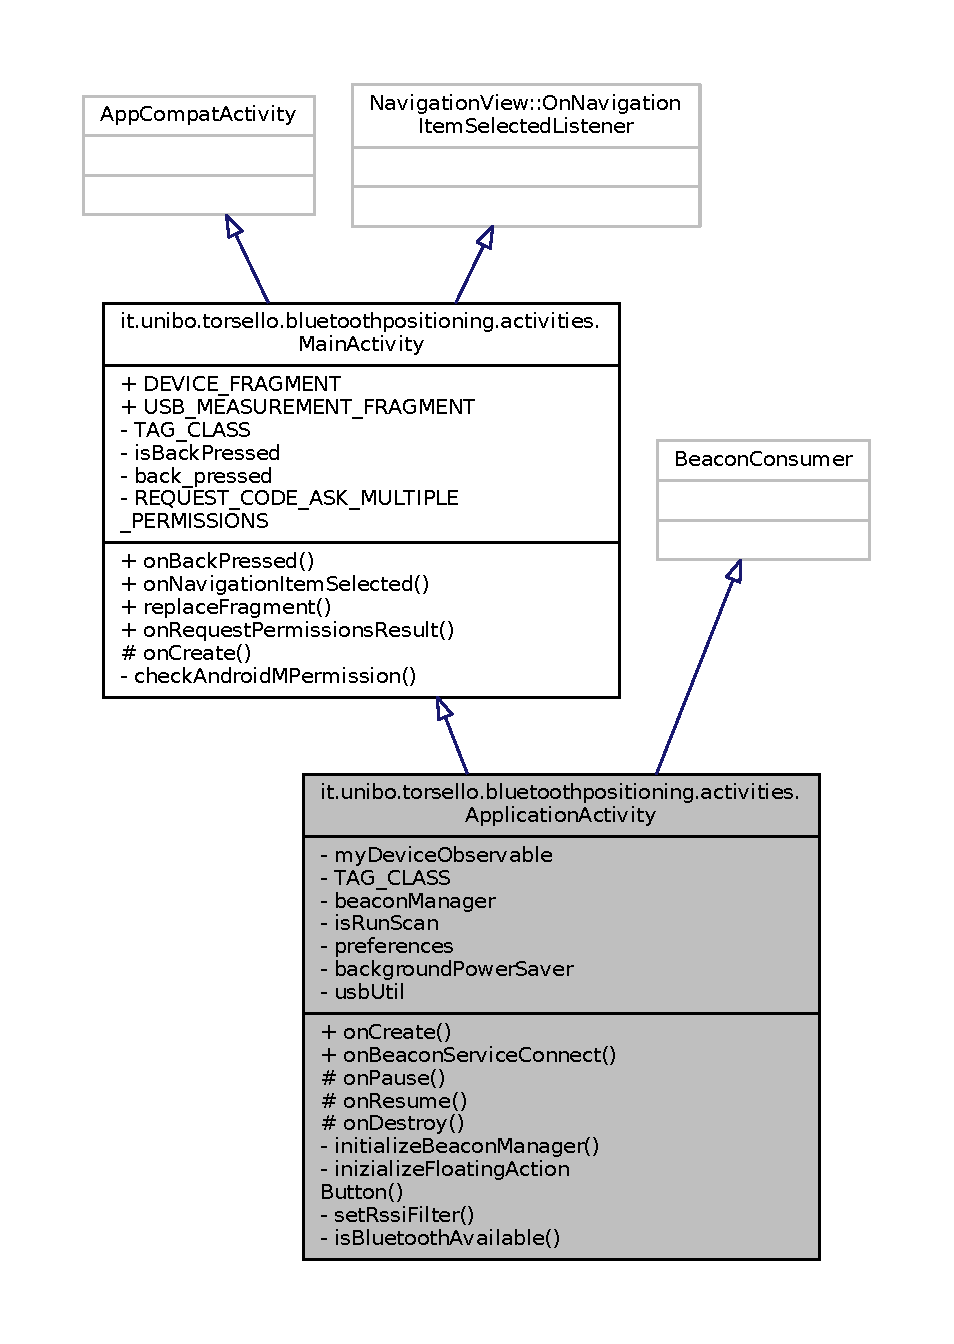
\includegraphics[width=350pt]{classit_1_1unibo_1_1torsello_1_1bluetoothpositioning_1_1activities_1_1ApplicationActivity__inherit__graph}
\end{center}
\end{figure}


Diagramma di collaborazione per it.\+unibo.\+torsello.\+bluetoothpositioning.\+activities.\+Application\+Activity\+:
\nopagebreak
\begin{figure}[H]
\begin{center}
\leavevmode
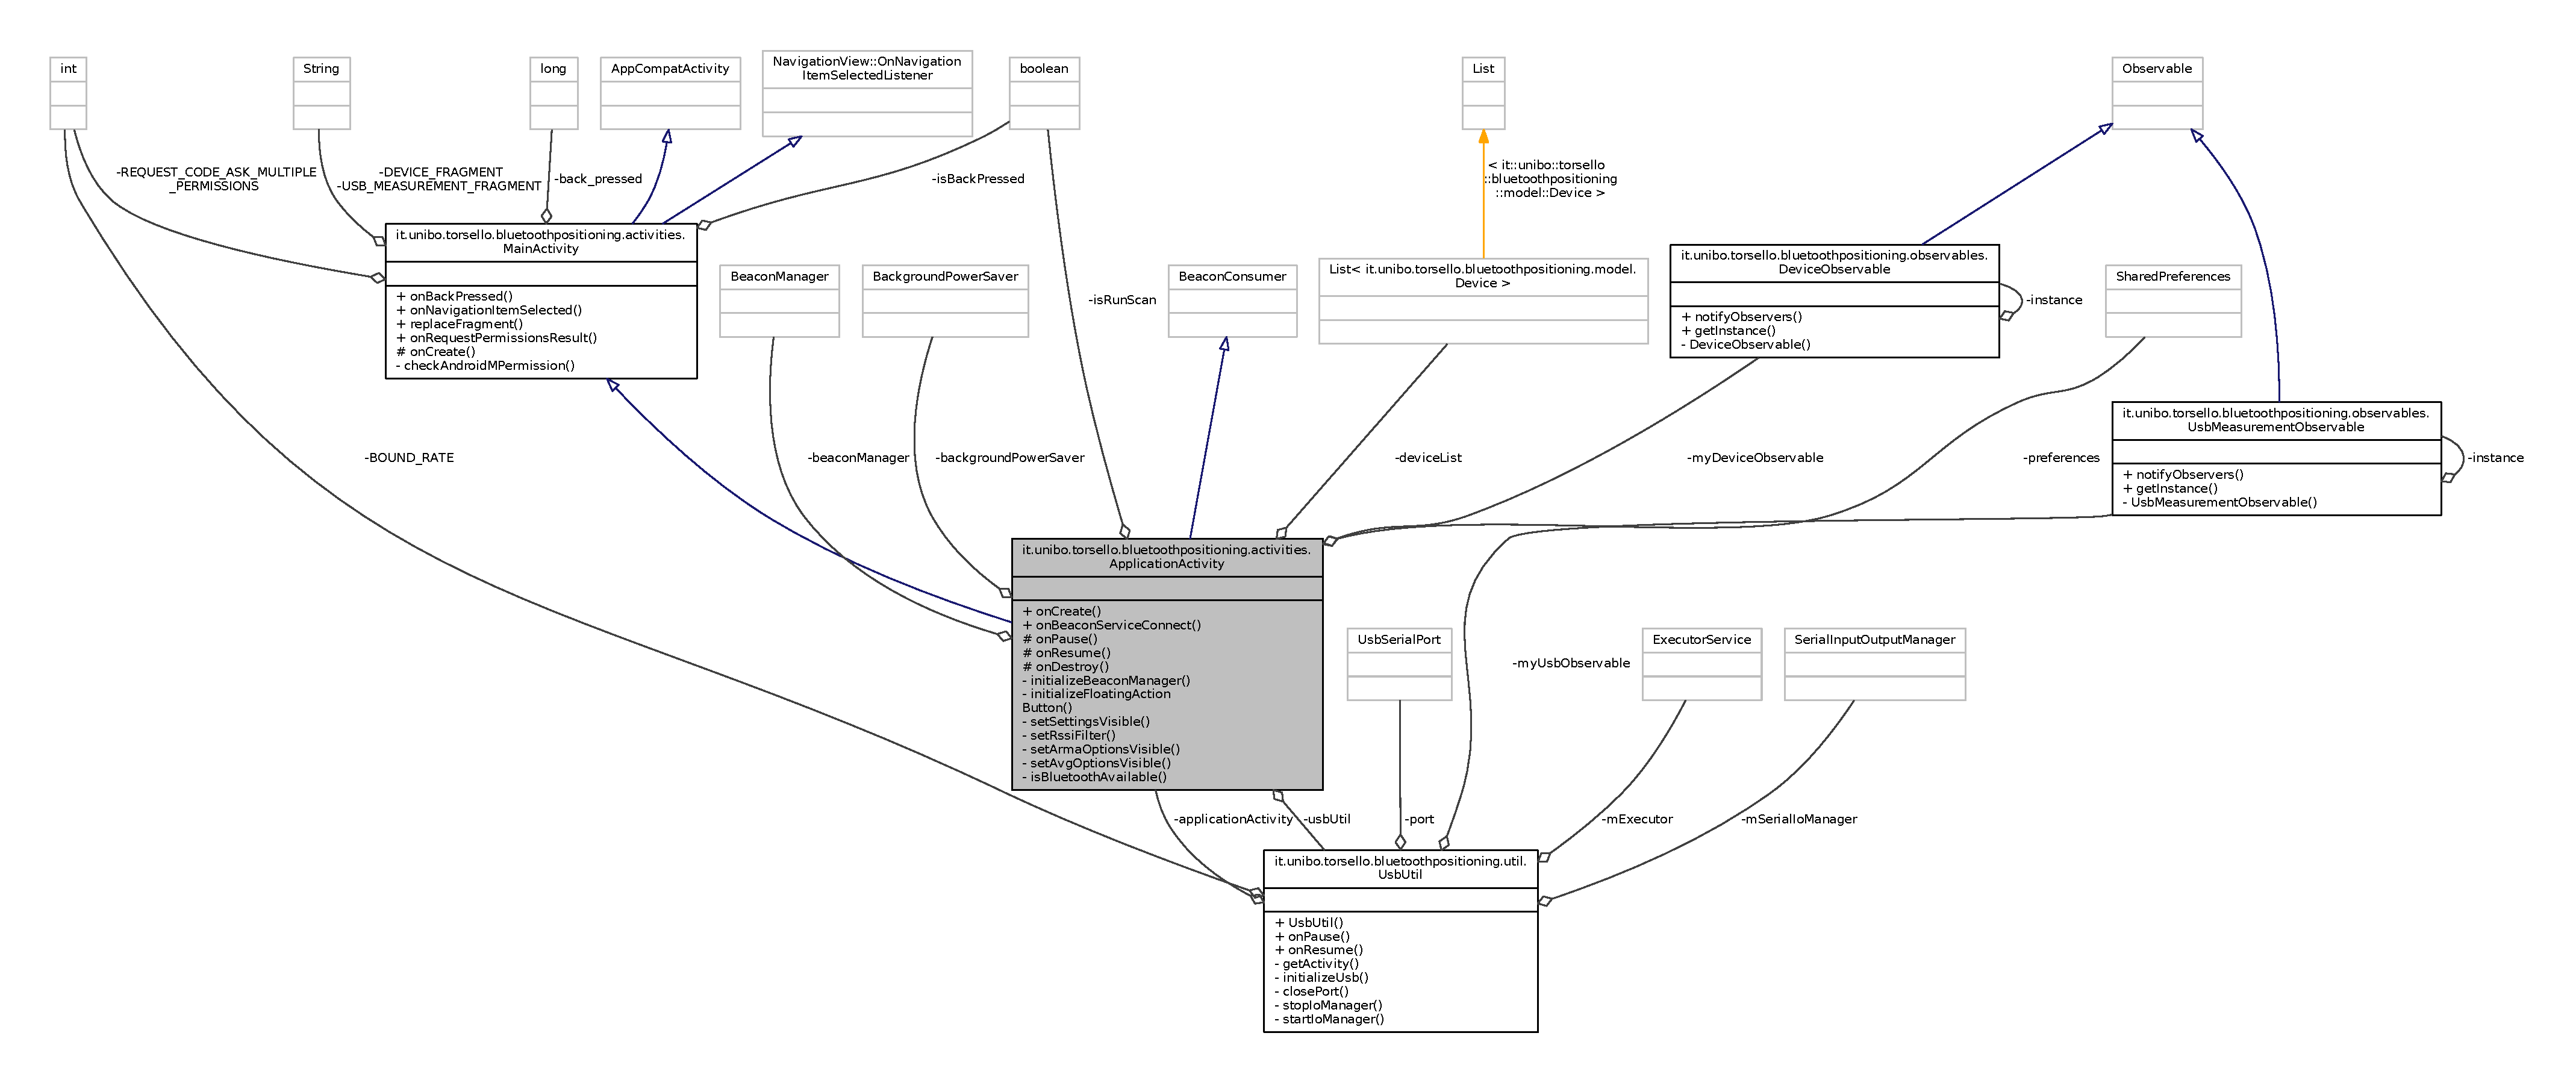
\includegraphics[width=350pt]{classit_1_1unibo_1_1torsello_1_1bluetoothpositioning_1_1activities_1_1ApplicationActivity__coll__graph}
\end{center}
\end{figure}
\subsubsection*{Membri pubblici}
\begin{DoxyCompactItemize}
\item 
void \hyperlink{classit_1_1unibo_1_1torsello_1_1bluetoothpositioning_1_1activities_1_1ApplicationActivity_a395bfa7ec016998b254b9e197ef8d754_a395bfa7ec016998b254b9e197ef8d754}{on\+Create} (Bundle saved\+Instance\+State)
\item 
void \hyperlink{classit_1_1unibo_1_1torsello_1_1bluetoothpositioning_1_1activities_1_1ApplicationActivity_a0cdfc0658ba462b43e9e6b94bab90da1_a0cdfc0658ba462b43e9e6b94bab90da1}{on\+Beacon\+Service\+Connect} ()
\end{DoxyCompactItemize}
\subsubsection*{Membri protetti}
\begin{DoxyCompactItemize}
\item 
void \hyperlink{classit_1_1unibo_1_1torsello_1_1bluetoothpositioning_1_1activities_1_1ApplicationActivity_a06ed1cf654098045b1317b25067af877_a06ed1cf654098045b1317b25067af877}{on\+Pause} ()
\item 
void \hyperlink{classit_1_1unibo_1_1torsello_1_1bluetoothpositioning_1_1activities_1_1ApplicationActivity_ad9e5c029636aac4d7baa2ca8695b3a18_ad9e5c029636aac4d7baa2ca8695b3a18}{on\+Resume} ()
\item 
void \hyperlink{classit_1_1unibo_1_1torsello_1_1bluetoothpositioning_1_1activities_1_1ApplicationActivity_a219ab2598668ab85771f3f8e3c6fec22_a219ab2598668ab85771f3f8e3c6fec22}{on\+Destroy} ()
\end{DoxyCompactItemize}
\subsubsection*{Membri privati}
\begin{DoxyCompactItemize}
\item 
void \hyperlink{classit_1_1unibo_1_1torsello_1_1bluetoothpositioning_1_1activities_1_1ApplicationActivity_a55d4f45ce163b9f613420686f6dfe1cf_a55d4f45ce163b9f613420686f6dfe1cf}{initialize\+Beacon\+Manager} ()
\item 
void \hyperlink{classit_1_1unibo_1_1torsello_1_1bluetoothpositioning_1_1activities_1_1ApplicationActivity_a290aa5909dd27864e0d7d772403ca900_a290aa5909dd27864e0d7d772403ca900}{inizialize\+Floating\+Action\+Button} ()
\item 
void \hyperlink{classit_1_1unibo_1_1torsello_1_1bluetoothpositioning_1_1activities_1_1ApplicationActivity_a8b2514096adfe574c15cc5317a45cd58_a8b2514096adfe574c15cc5317a45cd58}{set\+Rssi\+Filter} ()
\item 
boolean \hyperlink{classit_1_1unibo_1_1torsello_1_1bluetoothpositioning_1_1activities_1_1ApplicationActivity_abffd55741be864ad5b151c8f8c6d70ff_abffd55741be864ad5b151c8f8c6d70ff}{is\+Bluetooth\+Available} ()
\end{DoxyCompactItemize}
\subsubsection*{Attributi privati}
\begin{DoxyCompactItemize}
\item 
Beacon\+Manager \hyperlink{classit_1_1unibo_1_1torsello_1_1bluetoothpositioning_1_1activities_1_1ApplicationActivity_a973c37226a3dbba6016966c3555aff65_a973c37226a3dbba6016966c3555aff65}{beacon\+Manager}
\item 
\hyperlink{classit_1_1unibo_1_1torsello_1_1bluetoothpositioning_1_1observables_1_1DeviceObservable}{Device\+Observable} \hyperlink{classit_1_1unibo_1_1torsello_1_1bluetoothpositioning_1_1activities_1_1ApplicationActivity_aa6481e11e062d3539e6848f0790852b8_aa6481e11e062d3539e6848f0790852b8}{my\+Device\+Observable}
\item 
Shared\+Preferences \hyperlink{classit_1_1unibo_1_1torsello_1_1bluetoothpositioning_1_1activities_1_1ApplicationActivity_a3ee672ef79c268d0618ff3276c2e85f0_a3ee672ef79c268d0618ff3276c2e85f0}{preferences}
\item 
Background\+Power\+Saver \hyperlink{classit_1_1unibo_1_1torsello_1_1bluetoothpositioning_1_1activities_1_1ApplicationActivity_a85885639575161f4d73d4fc788f44ace_a85885639575161f4d73d4fc788f44ace}{background\+Power\+Saver}
\item 
\hyperlink{classit_1_1unibo_1_1torsello_1_1bluetoothpositioning_1_1util_1_1UsbUtil}{Usb\+Util} \hyperlink{classit_1_1unibo_1_1torsello_1_1bluetoothpositioning_1_1activities_1_1ApplicationActivity_abe62157d98c81406ae3d79dbc0fd9093_abe62157d98c81406ae3d79dbc0fd9093}{usb\+Util}
\item 
List$<$ \hyperlink{classit_1_1unibo_1_1torsello_1_1bluetoothpositioning_1_1model_1_1Device}{Device} $>$ \hyperlink{classit_1_1unibo_1_1torsello_1_1bluetoothpositioning_1_1activities_1_1ApplicationActivity_ad146f35cfee210f7191442658a235a2f_ad146f35cfee210f7191442658a235a2f}{device\+List}
\item 
boolean \hyperlink{classit_1_1unibo_1_1torsello_1_1bluetoothpositioning_1_1activities_1_1ApplicationActivity_a16080640c95a73d18c2b7ec21b785af1_a16080640c95a73d18c2b7ec21b785af1}{is\+Run\+Scan} = false
\end{DoxyCompactItemize}
\subsubsection*{Altri membri ereditati}


\subsubsection{Descrizione dettagliata}
Created by Federico Torsello. \href{mailto:federico.torsello@studio.unibo.it}{\tt federico.\+torsello@studio.\+unibo.\+it} 

\subsubsection{Documentazione delle funzioni membro}
\hypertarget{classit_1_1unibo_1_1torsello_1_1bluetoothpositioning_1_1activities_1_1ApplicationActivity_a55d4f45ce163b9f613420686f6dfe1cf_a55d4f45ce163b9f613420686f6dfe1cf}{}\label{classit_1_1unibo_1_1torsello_1_1bluetoothpositioning_1_1activities_1_1ApplicationActivity_a55d4f45ce163b9f613420686f6dfe1cf_a55d4f45ce163b9f613420686f6dfe1cf} 
\index{it\+::unibo\+::torsello\+::bluetoothpositioning\+::activities\+::\+Application\+Activity@{it\+::unibo\+::torsello\+::bluetoothpositioning\+::activities\+::\+Application\+Activity}!initialize\+Beacon\+Manager@{initialize\+Beacon\+Manager}}
\index{initialize\+Beacon\+Manager@{initialize\+Beacon\+Manager}!it\+::unibo\+::torsello\+::bluetoothpositioning\+::activities\+::\+Application\+Activity@{it\+::unibo\+::torsello\+::bluetoothpositioning\+::activities\+::\+Application\+Activity}}
\paragraph{\texorpdfstring{initialize\+Beacon\+Manager()}{initializeBeaconManager()}}
{\footnotesize\ttfamily void it.\+unibo.\+torsello.\+bluetoothpositioning.\+activities.\+Application\+Activity.\+initialize\+Beacon\+Manager (\begin{DoxyParamCaption}{ }\end{DoxyParamCaption})\hspace{0.3cm}{\ttfamily [private]}}


\begin{DoxyCode}
70                                            \{
71         \hyperlink{classit_1_1unibo_1_1torsello_1_1bluetoothpositioning_1_1activities_1_1ApplicationActivity_a973c37226a3dbba6016966c3555aff65_a973c37226a3dbba6016966c3555aff65}{beaconManager} = BeaconManager.getInstanceForApplication(\textcolor{keyword}{this});
72         \hyperlink{classit_1_1unibo_1_1torsello_1_1bluetoothpositioning_1_1activities_1_1ApplicationActivity_a973c37226a3dbba6016966c3555aff65_a973c37226a3dbba6016966c3555aff65}{beaconManager}.bind(\textcolor{keyword}{this});
73 
74         \textcolor{comment}{// Save battery whenever the application is not visible.}
75         \textcolor{comment}{// This reduces bluetooth power usage by about 60%}
76         \hyperlink{classit_1_1unibo_1_1torsello_1_1bluetoothpositioning_1_1activities_1_1ApplicationActivity_a85885639575161f4d73d4fc788f44ace_a85885639575161f4d73d4fc788f44ace}{backgroundPowerSaver} = \textcolor{keyword}{new} BackgroundPowerSaver(\textcolor{keyword}{this});
77 
78 \textcolor{comment}{//        Log.i("AltBeacon filter used:", BeaconManager.getRssiFilterImplClass().getSimpleName());}
79 
80         \textcolor{comment}{// for finding different type of beacon,}
81         \hyperlink{classit_1_1unibo_1_1torsello_1_1bluetoothpositioning_1_1activities_1_1ApplicationActivity_a973c37226a3dbba6016966c3555aff65_a973c37226a3dbba6016966c3555aff65}{beaconManager}.getBeaconParsers().clear();
82 
83         \textcolor{comment}{// Alt beacon}
84         \hyperlink{classit_1_1unibo_1_1torsello_1_1bluetoothpositioning_1_1activities_1_1ApplicationActivity_a973c37226a3dbba6016966c3555aff65_a973c37226a3dbba6016966c3555aff65}{beaconManager}.getBeaconParsers().add(\textcolor{keyword}{new} BeaconParser()
85                 .setBeaconLayout(BeaconParser.ALTBEACON\_LAYOUT));
86         \textcolor{comment}{// Detect the main identifier (UID) frame:}
87         \hyperlink{classit_1_1unibo_1_1torsello_1_1bluetoothpositioning_1_1activities_1_1ApplicationActivity_a973c37226a3dbba6016966c3555aff65_a973c37226a3dbba6016966c3555aff65}{beaconManager}.getBeaconParsers().add(\textcolor{keyword}{new} BeaconParser()
88                 .setBeaconLayout(BeaconParser.EDDYSTONE\_UID\_LAYOUT));
89         \textcolor{comment}{// Detect the telemetry (TLM) frame:}
90         \hyperlink{classit_1_1unibo_1_1torsello_1_1bluetoothpositioning_1_1activities_1_1ApplicationActivity_a973c37226a3dbba6016966c3555aff65_a973c37226a3dbba6016966c3555aff65}{beaconManager}.getBeaconParsers().add(\textcolor{keyword}{new} BeaconParser()
91                 .setBeaconLayout(BeaconParser.EDDYSTONE\_TLM\_LAYOUT));
92         \textcolor{comment}{// Detect the URL frame:}
93         \hyperlink{classit_1_1unibo_1_1torsello_1_1bluetoothpositioning_1_1activities_1_1ApplicationActivity_a973c37226a3dbba6016966c3555aff65_a973c37226a3dbba6016966c3555aff65}{beaconManager}.getBeaconParsers().add(\textcolor{keyword}{new} BeaconParser()
94                 .setBeaconLayout(BeaconParser.EDDYSTONE\_URL\_LAYOUT));
95         \textcolor{comment}{// Standard Apple iBeacon}
96         \hyperlink{classit_1_1unibo_1_1torsello_1_1bluetoothpositioning_1_1activities_1_1ApplicationActivity_a973c37226a3dbba6016966c3555aff65_a973c37226a3dbba6016966c3555aff65}{beaconManager}.getBeaconParsers().add(\textcolor{keyword}{new} BeaconParser()
97                 .setBeaconLayout(DeviceConstants.APPLE\_BEACON\_LAYOUT));
98         \textcolor{comment}{// Estimote Nearable}
99         \hyperlink{classit_1_1unibo_1_1torsello_1_1bluetoothpositioning_1_1activities_1_1ApplicationActivity_a973c37226a3dbba6016966c3555aff65_a973c37226a3dbba6016966c3555aff65}{beaconManager}.getBeaconParsers().add(\textcolor{keyword}{new} BeaconParser()
100                 .setBeaconLayout(DeviceConstants.ESTIMOTE\_NEARABLE\_LAYOUT));
101 
102         \hyperlink{classit_1_1unibo_1_1torsello_1_1bluetoothpositioning_1_1activities_1_1ApplicationActivity_a973c37226a3dbba6016966c3555aff65_a973c37226a3dbba6016966c3555aff65}{beaconManager}.setForegroundScanPeriod(250L);
103         \hyperlink{classit_1_1unibo_1_1torsello_1_1bluetoothpositioning_1_1activities_1_1ApplicationActivity_a973c37226a3dbba6016966c3555aff65_a973c37226a3dbba6016966c3555aff65}{beaconManager}.setForegroundBetweenScanPeriod(0L);
104         \hyperlink{classit_1_1unibo_1_1torsello_1_1bluetoothpositioning_1_1activities_1_1ApplicationActivity_a973c37226a3dbba6016966c3555aff65_a973c37226a3dbba6016966c3555aff65}{beaconManager}.setBackgroundScanPeriod(250L);
105         \hyperlink{classit_1_1unibo_1_1torsello_1_1bluetoothpositioning_1_1activities_1_1ApplicationActivity_a973c37226a3dbba6016966c3555aff65_a973c37226a3dbba6016966c3555aff65}{beaconManager}.setBackgroundBetweenScanPeriod(0L);
106 
107         \hyperlink{classit_1_1unibo_1_1torsello_1_1bluetoothpositioning_1_1activities_1_1ApplicationActivity_a973c37226a3dbba6016966c3555aff65_a973c37226a3dbba6016966c3555aff65}{beaconManager}.setMaxTrackingAge(1000);
108     \}
\end{DoxyCode}
\hypertarget{classit_1_1unibo_1_1torsello_1_1bluetoothpositioning_1_1activities_1_1ApplicationActivity_a290aa5909dd27864e0d7d772403ca900_a290aa5909dd27864e0d7d772403ca900}{}\label{classit_1_1unibo_1_1torsello_1_1bluetoothpositioning_1_1activities_1_1ApplicationActivity_a290aa5909dd27864e0d7d772403ca900_a290aa5909dd27864e0d7d772403ca900} 
\index{it\+::unibo\+::torsello\+::bluetoothpositioning\+::activities\+::\+Application\+Activity@{it\+::unibo\+::torsello\+::bluetoothpositioning\+::activities\+::\+Application\+Activity}!inizialize\+Floating\+Action\+Button@{inizialize\+Floating\+Action\+Button}}
\index{inizialize\+Floating\+Action\+Button@{inizialize\+Floating\+Action\+Button}!it\+::unibo\+::torsello\+::bluetoothpositioning\+::activities\+::\+Application\+Activity@{it\+::unibo\+::torsello\+::bluetoothpositioning\+::activities\+::\+Application\+Activity}}
\paragraph{\texorpdfstring{inizialize\+Floating\+Action\+Button()}{inizializeFloatingActionButton()}}
{\footnotesize\ttfamily void it.\+unibo.\+torsello.\+bluetoothpositioning.\+activities.\+Application\+Activity.\+inizialize\+Floating\+Action\+Button (\begin{DoxyParamCaption}{ }\end{DoxyParamCaption})\hspace{0.3cm}{\ttfamily [private]}}


\begin{DoxyCode}
110                                                   \{
111         \textcolor{keyword}{final} FloatingActionButton fab = (FloatingActionButton) findViewById(R.id.fab);
112         assert fab != null;
113         Snackbar.make(fab, R.string.snackBar\_start\_scanning, Snackbar.LENGTH\_LONG).show();
114         fab.setOnClickListener(\textcolor{keyword}{new} View.OnClickListener() \{
115             @Override
116             \textcolor{keyword}{public} \textcolor{keywordtype}{void} onClick(View view) \{
117 
118                 \textcolor{keywordflow}{if} (\hyperlink{classit_1_1unibo_1_1torsello_1_1bluetoothpositioning_1_1activities_1_1ApplicationActivity_abffd55741be864ad5b151c8f8c6d70ff_abffd55741be864ad5b151c8f8c6d70ff}{isBluetoothAvailable}()) \{
119 
120                     \hyperlink{classit_1_1unibo_1_1torsello_1_1bluetoothpositioning_1_1activities_1_1ApplicationActivity_a16080640c95a73d18c2b7ec21b785af1_a16080640c95a73d18c2b7ec21b785af1}{isRunScan} = !\hyperlink{classit_1_1unibo_1_1torsello_1_1bluetoothpositioning_1_1activities_1_1ApplicationActivity_a16080640c95a73d18c2b7ec21b785af1_a16080640c95a73d18c2b7ec21b785af1}{isRunScan};
121                     Region region = \textcolor{keyword}{new} Region(\textcolor{stringliteral}{"RegionId"}, null, null, null);
122 
123                     \textcolor{keywordflow}{if} (\hyperlink{classit_1_1unibo_1_1torsello_1_1bluetoothpositioning_1_1activities_1_1ApplicationActivity_a16080640c95a73d18c2b7ec21b785af1_a16080640c95a73d18c2b7ec21b785af1}{isRunScan}) \{
124                         fab.setImageResource(R.drawable.ic\_bluetooth\_searching\_white\_24dp);
125                         \textcolor{keywordflow}{try} \{
126                             \hyperlink{classit_1_1unibo_1_1torsello_1_1bluetoothpositioning_1_1activities_1_1ApplicationActivity_a973c37226a3dbba6016966c3555aff65_a973c37226a3dbba6016966c3555aff65}{beaconManager}.startRangingBeaconsInRegion(region);
127                         \} \textcolor{keywordflow}{catch} (RemoteException e) \{
128                             e.printStackTrace();
129                         \}
130                         Snackbar.make(view, R.string.snackBar\_scanning\_enabled,
131                                 Snackbar.LENGTH\_SHORT).show();
132                     \} \textcolor{keywordflow}{else} \{
133                         fab.setImageResource(R.drawable.ic\_bluetooth\_white\_24dp);
134                         \textcolor{keywordflow}{try} \{
135                             \hyperlink{classit_1_1unibo_1_1torsello_1_1bluetoothpositioning_1_1activities_1_1ApplicationActivity_a973c37226a3dbba6016966c3555aff65_a973c37226a3dbba6016966c3555aff65}{beaconManager}.stopRangingBeaconsInRegion(region);
136                         \} \textcolor{keywordflow}{catch} (RemoteException e) \{
137                             e.printStackTrace();
138                         \}
139                         Snackbar.make(view, R.string.snackBar\_scanning\_disabled,
140                                 Snackbar.LENGTH\_INDEFINITE).show();
141                     \}
142                 \}
143             \}
144         \});
145     \}
\end{DoxyCode}
\hypertarget{classit_1_1unibo_1_1torsello_1_1bluetoothpositioning_1_1activities_1_1ApplicationActivity_abffd55741be864ad5b151c8f8c6d70ff_abffd55741be864ad5b151c8f8c6d70ff}{}\label{classit_1_1unibo_1_1torsello_1_1bluetoothpositioning_1_1activities_1_1ApplicationActivity_abffd55741be864ad5b151c8f8c6d70ff_abffd55741be864ad5b151c8f8c6d70ff} 
\index{it\+::unibo\+::torsello\+::bluetoothpositioning\+::activities\+::\+Application\+Activity@{it\+::unibo\+::torsello\+::bluetoothpositioning\+::activities\+::\+Application\+Activity}!is\+Bluetooth\+Available@{is\+Bluetooth\+Available}}
\index{is\+Bluetooth\+Available@{is\+Bluetooth\+Available}!it\+::unibo\+::torsello\+::bluetoothpositioning\+::activities\+::\+Application\+Activity@{it\+::unibo\+::torsello\+::bluetoothpositioning\+::activities\+::\+Application\+Activity}}
\paragraph{\texorpdfstring{is\+Bluetooth\+Available()}{isBluetoothAvailable()}}
{\footnotesize\ttfamily boolean it.\+unibo.\+torsello.\+bluetoothpositioning.\+activities.\+Application\+Activity.\+is\+Bluetooth\+Available (\begin{DoxyParamCaption}{ }\end{DoxyParamCaption})\hspace{0.3cm}{\ttfamily [private]}}


\begin{DoxyCode}
250                                            \{
251 
252         \textcolor{keywordflow}{try} \{
253             \textcolor{keywordflow}{if} (!\hyperlink{classit_1_1unibo_1_1torsello_1_1bluetoothpositioning_1_1activities_1_1ApplicationActivity_a973c37226a3dbba6016966c3555aff65_a973c37226a3dbba6016966c3555aff65}{beaconManager}.checkAvailability()) \{
254 
255                 \textcolor{keyword}{final} FloatingActionButton fab = (FloatingActionButton) findViewById(R.id.fab);
256                 assert fab != null;
257 
258                 \textcolor{keyword}{new} AlertDialog.Builder(\textcolor{keyword}{this})
259                         .setTitle(R.string.dialog\_bluetooth\_title)
260                         .setMessage(R.string.dialog\_bluetooth\_text)
261                         .setPositiveButton(android.R.string.ok, null)
262                         .setOnDismissListener(\textcolor{keyword}{new} DialogInterface.OnDismissListener() \{
263                             @Override
264                             \textcolor{keyword}{public} \textcolor{keywordtype}{void} onDismiss(DialogInterface dialog) \{
265                                 fab.setImageResource(R.drawable.ic\_bluetooth\_white\_24dp);
266                                 BluetoothAdapter.getDefaultAdapter().enable();
267                             \}
268                         \}).show();
269                 fab.setImageResource(R.drawable.ic\_bluetooth\_disabled\_black\_24dp);
270                 \textcolor{keywordflow}{return} \textcolor{keyword}{false};
271             \}
272         \} \textcolor{keywordflow}{catch} (RuntimeException e) \{
273             e.getStackTrace();
274         \}
275         \textcolor{keywordflow}{return} \textcolor{keyword}{true};
276     \}
\end{DoxyCode}
\hypertarget{classit_1_1unibo_1_1torsello_1_1bluetoothpositioning_1_1activities_1_1ApplicationActivity_a0cdfc0658ba462b43e9e6b94bab90da1_a0cdfc0658ba462b43e9e6b94bab90da1}{}\label{classit_1_1unibo_1_1torsello_1_1bluetoothpositioning_1_1activities_1_1ApplicationActivity_a0cdfc0658ba462b43e9e6b94bab90da1_a0cdfc0658ba462b43e9e6b94bab90da1} 
\index{it\+::unibo\+::torsello\+::bluetoothpositioning\+::activities\+::\+Application\+Activity@{it\+::unibo\+::torsello\+::bluetoothpositioning\+::activities\+::\+Application\+Activity}!on\+Beacon\+Service\+Connect@{on\+Beacon\+Service\+Connect}}
\index{on\+Beacon\+Service\+Connect@{on\+Beacon\+Service\+Connect}!it\+::unibo\+::torsello\+::bluetoothpositioning\+::activities\+::\+Application\+Activity@{it\+::unibo\+::torsello\+::bluetoothpositioning\+::activities\+::\+Application\+Activity}}
\paragraph{\texorpdfstring{on\+Beacon\+Service\+Connect()}{onBeaconServiceConnect()}}
{\footnotesize\ttfamily void it.\+unibo.\+torsello.\+bluetoothpositioning.\+activities.\+Application\+Activity.\+on\+Beacon\+Service\+Connect (\begin{DoxyParamCaption}{ }\end{DoxyParamCaption})}


\begin{DoxyCode}
148                                          \{
149 
150         \textcolor{keywordflow}{try} \{
151             \hyperlink{classit_1_1unibo_1_1torsello_1_1bluetoothpositioning_1_1activities_1_1ApplicationActivity_a973c37226a3dbba6016966c3555aff65_a973c37226a3dbba6016966c3555aff65}{beaconManager}.updateScanPeriods();
152         \} \textcolor{keywordflow}{catch} (RemoteException e) \{
153             e.printStackTrace();
154         \}
155 
156         \hyperlink{classit_1_1unibo_1_1torsello_1_1bluetoothpositioning_1_1activities_1_1ApplicationActivity_a973c37226a3dbba6016966c3555aff65_a973c37226a3dbba6016966c3555aff65}{beaconManager}.addRangeNotifier(\textcolor{keyword}{new} RangeNotifier() \{
157             @Override
158             \textcolor{keyword}{public} \textcolor{keywordtype}{void} didRangeBeaconsInRegion(\textcolor{keyword}{final} Collection<Beacon> beacons, Region region) \{
159 
160                 \hyperlink{classit_1_1unibo_1_1torsello_1_1bluetoothpositioning_1_1activities_1_1ApplicationActivity_a8b2514096adfe574c15cc5317a45cd58_a8b2514096adfe574c15cc5317a45cd58}{setRssiFilter}();
161 
162                 \textcolor{keywordflow}{for} (Beacon b : beacons) \{
163 
164                     \textcolor{comment}{// take from the list the device}
165                     Device device = DeviceConstants.DEVICE\_MAP.get(b.getBluetoothAddress());
166 
167                     \textcolor{keywordflow}{if} (device != null) \{ \textcolor{comment}{// useful only if DEVICE\_MAP is empty}
168                         \textcolor{keywordtype}{double} processNoise = \hyperlink{classit_1_1unibo_1_1torsello_1_1bluetoothpositioning_1_1activities_1_1ApplicationActivity_a3ee672ef79c268d0618ff3276c2e85f0_a3ee672ef79c268d0618ff3276c2e85f0}{preferences}.getFloat(SettingConstants.
      KALMAN\_NOISE\_VALUE, 0);
169                         device.setBeacon(b);
170                         device.updateDistance(processNoise);
171 
172                         \textcolor{keywordflow}{if} (!\hyperlink{classit_1_1unibo_1_1torsello_1_1bluetoothpositioning_1_1activities_1_1ApplicationActivity_ad146f35cfee210f7191442658a235a2f_ad146f35cfee210f7191442658a235a2f}{deviceList}.contains(device)) \{
173                             \hyperlink{classit_1_1unibo_1_1torsello_1_1bluetoothpositioning_1_1activities_1_1ApplicationActivity_ad146f35cfee210f7191442658a235a2f_ad146f35cfee210f7191442658a235a2f}{deviceList}.add(device);
174                         \}
175                     \}
176                 \}
177 
178                 \textcolor{keyword}{new} Thread(\textcolor{keyword}{new} Runnable() \{
179                     @Override
180                     \textcolor{keyword}{public} \textcolor{keywordtype}{void} run() \{
181                         runOnUiThread(\textcolor{keyword}{new} Runnable() \{
182 
183                             @Override
184                             \textcolor{keyword}{public} \textcolor{keywordtype}{void} run() \{
185                                 \hyperlink{classit_1_1unibo_1_1torsello_1_1bluetoothpositioning_1_1activities_1_1ApplicationActivity_aa6481e11e062d3539e6848f0790852b8_aa6481e11e062d3539e6848f0790852b8}{myDeviceObservable}.
      \hyperlink{classit_1_1unibo_1_1torsello_1_1bluetoothpositioning_1_1observables_1_1DeviceObservable_aaf183e537e44cbd114c8eb76432da191_aaf183e537e44cbd114c8eb76432da191}{notifyObservers}(\hyperlink{classit_1_1unibo_1_1torsello_1_1bluetoothpositioning_1_1activities_1_1ApplicationActivity_ad146f35cfee210f7191442658a235a2f_ad146f35cfee210f7191442658a235a2f}{deviceList});
186                             \}
187                         \});
188                     \}
189                 \}).start();
190             \}
191         \});
192     \}
\end{DoxyCode}
\hypertarget{classit_1_1unibo_1_1torsello_1_1bluetoothpositioning_1_1activities_1_1ApplicationActivity_a395bfa7ec016998b254b9e197ef8d754_a395bfa7ec016998b254b9e197ef8d754}{}\label{classit_1_1unibo_1_1torsello_1_1bluetoothpositioning_1_1activities_1_1ApplicationActivity_a395bfa7ec016998b254b9e197ef8d754_a395bfa7ec016998b254b9e197ef8d754} 
\index{it\+::unibo\+::torsello\+::bluetoothpositioning\+::activities\+::\+Application\+Activity@{it\+::unibo\+::torsello\+::bluetoothpositioning\+::activities\+::\+Application\+Activity}!on\+Create@{on\+Create}}
\index{on\+Create@{on\+Create}!it\+::unibo\+::torsello\+::bluetoothpositioning\+::activities\+::\+Application\+Activity@{it\+::unibo\+::torsello\+::bluetoothpositioning\+::activities\+::\+Application\+Activity}}
\paragraph{\texorpdfstring{on\+Create()}{onCreate()}}
{\footnotesize\ttfamily void it.\+unibo.\+torsello.\+bluetoothpositioning.\+activities.\+Application\+Activity.\+on\+Create (\begin{DoxyParamCaption}\item[{Bundle}]{saved\+Instance\+State }\end{DoxyParamCaption})}


\begin{DoxyCode}
54                                                     \{
55         super.onCreate(savedInstanceState);
56 
57         \hyperlink{classit_1_1unibo_1_1torsello_1_1bluetoothpositioning_1_1activities_1_1ApplicationActivity_ad146f35cfee210f7191442658a235a2f_ad146f35cfee210f7191442658a235a2f}{deviceList} = \textcolor{keyword}{new} ArrayList<>();
58 
59         \hyperlink{classit_1_1unibo_1_1torsello_1_1bluetoothpositioning_1_1activities_1_1ApplicationActivity_aa6481e11e062d3539e6848f0790852b8_aa6481e11e062d3539e6848f0790852b8}{myDeviceObservable} = DeviceObservable.\hyperlink{classit_1_1unibo_1_1torsello_1_1bluetoothpositioning_1_1observables_1_1DeviceObservable_ab16792c5848440646624b2a41553954a_ab16792c5848440646624b2a41553954a}{getInstance}();
60 
61         \hyperlink{classit_1_1unibo_1_1torsello_1_1bluetoothpositioning_1_1activities_1_1ApplicationActivity_a3ee672ef79c268d0618ff3276c2e85f0_a3ee672ef79c268d0618ff3276c2e85f0}{preferences} = getSharedPreferences(SettingConstants.SETTINGS\_PREFERENCES, 0);
62 
63         \hyperlink{classit_1_1unibo_1_1torsello_1_1bluetoothpositioning_1_1activities_1_1ApplicationActivity_abe62157d98c81406ae3d79dbc0fd9093_abe62157d98c81406ae3d79dbc0fd9093}{usbUtil} = \textcolor{keyword}{new} UsbUtil(\textcolor{keyword}{this});
64 
65         \hyperlink{classit_1_1unibo_1_1torsello_1_1bluetoothpositioning_1_1activities_1_1ApplicationActivity_a55d4f45ce163b9f613420686f6dfe1cf_a55d4f45ce163b9f613420686f6dfe1cf}{initializeBeaconManager}();
66 
67         \hyperlink{classit_1_1unibo_1_1torsello_1_1bluetoothpositioning_1_1activities_1_1ApplicationActivity_a290aa5909dd27864e0d7d772403ca900_a290aa5909dd27864e0d7d772403ca900}{inizializeFloatingActionButton}();
68     \}
\end{DoxyCode}
\hypertarget{classit_1_1unibo_1_1torsello_1_1bluetoothpositioning_1_1activities_1_1ApplicationActivity_a219ab2598668ab85771f3f8e3c6fec22_a219ab2598668ab85771f3f8e3c6fec22}{}\label{classit_1_1unibo_1_1torsello_1_1bluetoothpositioning_1_1activities_1_1ApplicationActivity_a219ab2598668ab85771f3f8e3c6fec22_a219ab2598668ab85771f3f8e3c6fec22} 
\index{it\+::unibo\+::torsello\+::bluetoothpositioning\+::activities\+::\+Application\+Activity@{it\+::unibo\+::torsello\+::bluetoothpositioning\+::activities\+::\+Application\+Activity}!on\+Destroy@{on\+Destroy}}
\index{on\+Destroy@{on\+Destroy}!it\+::unibo\+::torsello\+::bluetoothpositioning\+::activities\+::\+Application\+Activity@{it\+::unibo\+::torsello\+::bluetoothpositioning\+::activities\+::\+Application\+Activity}}
\paragraph{\texorpdfstring{on\+Destroy()}{onDestroy()}}
{\footnotesize\ttfamily void it.\+unibo.\+torsello.\+bluetoothpositioning.\+activities.\+Application\+Activity.\+on\+Destroy (\begin{DoxyParamCaption}{ }\end{DoxyParamCaption})\hspace{0.3cm}{\ttfamily [protected]}}


\begin{DoxyCode}
241                                \{
242         \textcolor{keywordflow}{if} (\hyperlink{classit_1_1unibo_1_1torsello_1_1bluetoothpositioning_1_1activities_1_1ApplicationActivity_a973c37226a3dbba6016966c3555aff65_a973c37226a3dbba6016966c3555aff65}{beaconManager}.isBound(\textcolor{keyword}{this})) \{
243             \hyperlink{classit_1_1unibo_1_1torsello_1_1bluetoothpositioning_1_1activities_1_1ApplicationActivity_a973c37226a3dbba6016966c3555aff65_a973c37226a3dbba6016966c3555aff65}{beaconManager}.unbind(\textcolor{keyword}{this});
244             \hyperlink{classit_1_1unibo_1_1torsello_1_1bluetoothpositioning_1_1activities_1_1ApplicationActivity_a85885639575161f4d73d4fc788f44ace_a85885639575161f4d73d4fc788f44ace}{backgroundPowerSaver}.onActivityDestroyed(\textcolor{keyword}{this});
245         \}
246 
247         super.onDestroy();
248     \}
\end{DoxyCode}
\hypertarget{classit_1_1unibo_1_1torsello_1_1bluetoothpositioning_1_1activities_1_1ApplicationActivity_a06ed1cf654098045b1317b25067af877_a06ed1cf654098045b1317b25067af877}{}\label{classit_1_1unibo_1_1torsello_1_1bluetoothpositioning_1_1activities_1_1ApplicationActivity_a06ed1cf654098045b1317b25067af877_a06ed1cf654098045b1317b25067af877} 
\index{it\+::unibo\+::torsello\+::bluetoothpositioning\+::activities\+::\+Application\+Activity@{it\+::unibo\+::torsello\+::bluetoothpositioning\+::activities\+::\+Application\+Activity}!on\+Pause@{on\+Pause}}
\index{on\+Pause@{on\+Pause}!it\+::unibo\+::torsello\+::bluetoothpositioning\+::activities\+::\+Application\+Activity@{it\+::unibo\+::torsello\+::bluetoothpositioning\+::activities\+::\+Application\+Activity}}
\paragraph{\texorpdfstring{on\+Pause()}{onPause()}}
{\footnotesize\ttfamily void it.\+unibo.\+torsello.\+bluetoothpositioning.\+activities.\+Application\+Activity.\+on\+Pause (\begin{DoxyParamCaption}{ }\end{DoxyParamCaption})\hspace{0.3cm}{\ttfamily [protected]}}


\begin{DoxyCode}
214                              \{
215         \textcolor{keywordflow}{if} (\hyperlink{classit_1_1unibo_1_1torsello_1_1bluetoothpositioning_1_1activities_1_1ApplicationActivity_a973c37226a3dbba6016966c3555aff65_a973c37226a3dbba6016966c3555aff65}{beaconManager}.isBound(\textcolor{keyword}{this})) \{
216             \hyperlink{classit_1_1unibo_1_1torsello_1_1bluetoothpositioning_1_1activities_1_1ApplicationActivity_a973c37226a3dbba6016966c3555aff65_a973c37226a3dbba6016966c3555aff65}{beaconManager}.setBackgroundMode(\textcolor{keyword}{true});
217             \hyperlink{classit_1_1unibo_1_1torsello_1_1bluetoothpositioning_1_1activities_1_1ApplicationActivity_a85885639575161f4d73d4fc788f44ace_a85885639575161f4d73d4fc788f44ace}{backgroundPowerSaver}.onActivityPaused(\textcolor{keyword}{this});
218         \}
219 
220         \hyperlink{classit_1_1unibo_1_1torsello_1_1bluetoothpositioning_1_1activities_1_1ApplicationActivity_abe62157d98c81406ae3d79dbc0fd9093_abe62157d98c81406ae3d79dbc0fd9093}{usbUtil}.\hyperlink{classit_1_1unibo_1_1torsello_1_1bluetoothpositioning_1_1util_1_1UsbUtil_ab4f2c73fa6b776c9d4967ff89da0d8ca_ab4f2c73fa6b776c9d4967ff89da0d8ca}{onPause}();
221 
222         super.onPause();
223     \}
\end{DoxyCode}
\hypertarget{classit_1_1unibo_1_1torsello_1_1bluetoothpositioning_1_1activities_1_1ApplicationActivity_ad9e5c029636aac4d7baa2ca8695b3a18_ad9e5c029636aac4d7baa2ca8695b3a18}{}\label{classit_1_1unibo_1_1torsello_1_1bluetoothpositioning_1_1activities_1_1ApplicationActivity_ad9e5c029636aac4d7baa2ca8695b3a18_ad9e5c029636aac4d7baa2ca8695b3a18} 
\index{it\+::unibo\+::torsello\+::bluetoothpositioning\+::activities\+::\+Application\+Activity@{it\+::unibo\+::torsello\+::bluetoothpositioning\+::activities\+::\+Application\+Activity}!on\+Resume@{on\+Resume}}
\index{on\+Resume@{on\+Resume}!it\+::unibo\+::torsello\+::bluetoothpositioning\+::activities\+::\+Application\+Activity@{it\+::unibo\+::torsello\+::bluetoothpositioning\+::activities\+::\+Application\+Activity}}
\paragraph{\texorpdfstring{on\+Resume()}{onResume()}}
{\footnotesize\ttfamily void it.\+unibo.\+torsello.\+bluetoothpositioning.\+activities.\+Application\+Activity.\+on\+Resume (\begin{DoxyParamCaption}{ }\end{DoxyParamCaption})\hspace{0.3cm}{\ttfamily [protected]}}


\begin{DoxyCode}
226                               \{
227         super.onResume();
228 
229         \textcolor{keywordflow}{if} (\hyperlink{classit_1_1unibo_1_1torsello_1_1bluetoothpositioning_1_1activities_1_1ApplicationActivity_a973c37226a3dbba6016966c3555aff65_a973c37226a3dbba6016966c3555aff65}{beaconManager}.isBound(\textcolor{keyword}{this})) \{
230             \hyperlink{classit_1_1unibo_1_1torsello_1_1bluetoothpositioning_1_1activities_1_1ApplicationActivity_a973c37226a3dbba6016966c3555aff65_a973c37226a3dbba6016966c3555aff65}{beaconManager}.setBackgroundMode(\textcolor{keyword}{false});
231             \hyperlink{classit_1_1unibo_1_1torsello_1_1bluetoothpositioning_1_1activities_1_1ApplicationActivity_a85885639575161f4d73d4fc788f44ace_a85885639575161f4d73d4fc788f44ace}{backgroundPowerSaver}.onActivityResumed(\textcolor{keyword}{this});
232         \}
233 
234         \hyperlink{classit_1_1unibo_1_1torsello_1_1bluetoothpositioning_1_1activities_1_1ApplicationActivity_abffd55741be864ad5b151c8f8c6d70ff_abffd55741be864ad5b151c8f8c6d70ff}{isBluetoothAvailable}();
235 
236         \hyperlink{classit_1_1unibo_1_1torsello_1_1bluetoothpositioning_1_1activities_1_1ApplicationActivity_abe62157d98c81406ae3d79dbc0fd9093_abe62157d98c81406ae3d79dbc0fd9093}{usbUtil}.\hyperlink{classit_1_1unibo_1_1torsello_1_1bluetoothpositioning_1_1util_1_1UsbUtil_ae814610c8dc793fea3a9a314fb26e3cb_ae814610c8dc793fea3a9a314fb26e3cb}{onResume}();
237 
238     \}
\end{DoxyCode}
\hypertarget{classit_1_1unibo_1_1torsello_1_1bluetoothpositioning_1_1activities_1_1ApplicationActivity_a8b2514096adfe574c15cc5317a45cd58_a8b2514096adfe574c15cc5317a45cd58}{}\label{classit_1_1unibo_1_1torsello_1_1bluetoothpositioning_1_1activities_1_1ApplicationActivity_a8b2514096adfe574c15cc5317a45cd58_a8b2514096adfe574c15cc5317a45cd58} 
\index{it\+::unibo\+::torsello\+::bluetoothpositioning\+::activities\+::\+Application\+Activity@{it\+::unibo\+::torsello\+::bluetoothpositioning\+::activities\+::\+Application\+Activity}!set\+Rssi\+Filter@{set\+Rssi\+Filter}}
\index{set\+Rssi\+Filter@{set\+Rssi\+Filter}!it\+::unibo\+::torsello\+::bluetoothpositioning\+::activities\+::\+Application\+Activity@{it\+::unibo\+::torsello\+::bluetoothpositioning\+::activities\+::\+Application\+Activity}}
\paragraph{\texorpdfstring{set\+Rssi\+Filter()}{setRssiFilter()}}
{\footnotesize\ttfamily void it.\+unibo.\+torsello.\+bluetoothpositioning.\+activities.\+Application\+Activity.\+set\+Rssi\+Filter (\begin{DoxyParamCaption}{ }\end{DoxyParamCaption})\hspace{0.3cm}{\ttfamily [private]}}


\begin{DoxyCode}
194                                  \{
195 
196         \textcolor{keywordtype}{int} sorting = \hyperlink{classit_1_1unibo_1_1torsello_1_1bluetoothpositioning_1_1activities_1_1ApplicationActivity_a3ee672ef79c268d0618ff3276c2e85f0_a3ee672ef79c268d0618ff3276c2e85f0}{preferences}.getInt(SettingConstants.FILTER\_RSSI, 0);
197         \textcolor{keywordflow}{switch} (sorting) \{
198             \textcolor{keywordflow}{case} 0:
199             \textcolor{keywordflow}{case} R.id.radioButton\_no\_rssi\_filtering:
200                 MyArmaRssiFilter.enableArmaFilter(\textcolor{keyword}{false});
201                 BeaconManager.setRssiFilterImplClass(MyArmaRssiFilter.class);
202                 \textcolor{keywordflow}{break};
203             \textcolor{keywordflow}{case} R.id.radioButton\_arma\_rssi\_filter:
204                 MyArmaRssiFilter.enableArmaFilter(\textcolor{keyword}{true});
205                 BeaconManager.setRssiFilterImplClass(MyArmaRssiFilter.class);
206                 \textcolor{keywordflow}{break};
207             \textcolor{keywordflow}{case} R.id.radioButton\_average\_rssi\_filter:
208                 BeaconManager.setRssiFilterImplClass(RunningAverageRssiFilter.class);
209                 \textcolor{keywordflow}{break};
210         \}
211     \}
\end{DoxyCode}


\subsubsection{Documentazione dei membri dato}
\hypertarget{classit_1_1unibo_1_1torsello_1_1bluetoothpositioning_1_1activities_1_1ApplicationActivity_a85885639575161f4d73d4fc788f44ace_a85885639575161f4d73d4fc788f44ace}{}\label{classit_1_1unibo_1_1torsello_1_1bluetoothpositioning_1_1activities_1_1ApplicationActivity_a85885639575161f4d73d4fc788f44ace_a85885639575161f4d73d4fc788f44ace} 
\index{it\+::unibo\+::torsello\+::bluetoothpositioning\+::activities\+::\+Application\+Activity@{it\+::unibo\+::torsello\+::bluetoothpositioning\+::activities\+::\+Application\+Activity}!background\+Power\+Saver@{background\+Power\+Saver}}
\index{background\+Power\+Saver@{background\+Power\+Saver}!it\+::unibo\+::torsello\+::bluetoothpositioning\+::activities\+::\+Application\+Activity@{it\+::unibo\+::torsello\+::bluetoothpositioning\+::activities\+::\+Application\+Activity}}
\paragraph{\texorpdfstring{background\+Power\+Saver}{backgroundPowerSaver}}
{\footnotesize\ttfamily Background\+Power\+Saver it.\+unibo.\+torsello.\+bluetoothpositioning.\+activities.\+Application\+Activity.\+background\+Power\+Saver\hspace{0.3cm}{\ttfamily [private]}}

\hypertarget{classit_1_1unibo_1_1torsello_1_1bluetoothpositioning_1_1activities_1_1ApplicationActivity_a973c37226a3dbba6016966c3555aff65_a973c37226a3dbba6016966c3555aff65}{}\label{classit_1_1unibo_1_1torsello_1_1bluetoothpositioning_1_1activities_1_1ApplicationActivity_a973c37226a3dbba6016966c3555aff65_a973c37226a3dbba6016966c3555aff65} 
\index{it\+::unibo\+::torsello\+::bluetoothpositioning\+::activities\+::\+Application\+Activity@{it\+::unibo\+::torsello\+::bluetoothpositioning\+::activities\+::\+Application\+Activity}!beacon\+Manager@{beacon\+Manager}}
\index{beacon\+Manager@{beacon\+Manager}!it\+::unibo\+::torsello\+::bluetoothpositioning\+::activities\+::\+Application\+Activity@{it\+::unibo\+::torsello\+::bluetoothpositioning\+::activities\+::\+Application\+Activity}}
\paragraph{\texorpdfstring{beacon\+Manager}{beaconManager}}
{\footnotesize\ttfamily Beacon\+Manager it.\+unibo.\+torsello.\+bluetoothpositioning.\+activities.\+Application\+Activity.\+beacon\+Manager\hspace{0.3cm}{\ttfamily [private]}}

\hypertarget{classit_1_1unibo_1_1torsello_1_1bluetoothpositioning_1_1activities_1_1ApplicationActivity_ad146f35cfee210f7191442658a235a2f_ad146f35cfee210f7191442658a235a2f}{}\label{classit_1_1unibo_1_1torsello_1_1bluetoothpositioning_1_1activities_1_1ApplicationActivity_ad146f35cfee210f7191442658a235a2f_ad146f35cfee210f7191442658a235a2f} 
\index{it\+::unibo\+::torsello\+::bluetoothpositioning\+::activities\+::\+Application\+Activity@{it\+::unibo\+::torsello\+::bluetoothpositioning\+::activities\+::\+Application\+Activity}!device\+List@{device\+List}}
\index{device\+List@{device\+List}!it\+::unibo\+::torsello\+::bluetoothpositioning\+::activities\+::\+Application\+Activity@{it\+::unibo\+::torsello\+::bluetoothpositioning\+::activities\+::\+Application\+Activity}}
\paragraph{\texorpdfstring{device\+List}{deviceList}}
{\footnotesize\ttfamily List$<$\hyperlink{classit_1_1unibo_1_1torsello_1_1bluetoothpositioning_1_1model_1_1Device}{Device}$>$ it.\+unibo.\+torsello.\+bluetoothpositioning.\+activities.\+Application\+Activity.\+device\+List\hspace{0.3cm}{\ttfamily [private]}}

\hypertarget{classit_1_1unibo_1_1torsello_1_1bluetoothpositioning_1_1activities_1_1ApplicationActivity_a16080640c95a73d18c2b7ec21b785af1_a16080640c95a73d18c2b7ec21b785af1}{}\label{classit_1_1unibo_1_1torsello_1_1bluetoothpositioning_1_1activities_1_1ApplicationActivity_a16080640c95a73d18c2b7ec21b785af1_a16080640c95a73d18c2b7ec21b785af1} 
\index{it\+::unibo\+::torsello\+::bluetoothpositioning\+::activities\+::\+Application\+Activity@{it\+::unibo\+::torsello\+::bluetoothpositioning\+::activities\+::\+Application\+Activity}!is\+Run\+Scan@{is\+Run\+Scan}}
\index{is\+Run\+Scan@{is\+Run\+Scan}!it\+::unibo\+::torsello\+::bluetoothpositioning\+::activities\+::\+Application\+Activity@{it\+::unibo\+::torsello\+::bluetoothpositioning\+::activities\+::\+Application\+Activity}}
\paragraph{\texorpdfstring{is\+Run\+Scan}{isRunScan}}
{\footnotesize\ttfamily boolean it.\+unibo.\+torsello.\+bluetoothpositioning.\+activities.\+Application\+Activity.\+is\+Run\+Scan = false\hspace{0.3cm}{\ttfamily [private]}}

\hypertarget{classit_1_1unibo_1_1torsello_1_1bluetoothpositioning_1_1activities_1_1ApplicationActivity_aa6481e11e062d3539e6848f0790852b8_aa6481e11e062d3539e6848f0790852b8}{}\label{classit_1_1unibo_1_1torsello_1_1bluetoothpositioning_1_1activities_1_1ApplicationActivity_aa6481e11e062d3539e6848f0790852b8_aa6481e11e062d3539e6848f0790852b8} 
\index{it\+::unibo\+::torsello\+::bluetoothpositioning\+::activities\+::\+Application\+Activity@{it\+::unibo\+::torsello\+::bluetoothpositioning\+::activities\+::\+Application\+Activity}!my\+Device\+Observable@{my\+Device\+Observable}}
\index{my\+Device\+Observable@{my\+Device\+Observable}!it\+::unibo\+::torsello\+::bluetoothpositioning\+::activities\+::\+Application\+Activity@{it\+::unibo\+::torsello\+::bluetoothpositioning\+::activities\+::\+Application\+Activity}}
\paragraph{\texorpdfstring{my\+Device\+Observable}{myDeviceObservable}}
{\footnotesize\ttfamily \hyperlink{classit_1_1unibo_1_1torsello_1_1bluetoothpositioning_1_1observables_1_1DeviceObservable}{Device\+Observable} it.\+unibo.\+torsello.\+bluetoothpositioning.\+activities.\+Application\+Activity.\+my\+Device\+Observable\hspace{0.3cm}{\ttfamily [private]}}

\hypertarget{classit_1_1unibo_1_1torsello_1_1bluetoothpositioning_1_1activities_1_1ApplicationActivity_a3ee672ef79c268d0618ff3276c2e85f0_a3ee672ef79c268d0618ff3276c2e85f0}{}\label{classit_1_1unibo_1_1torsello_1_1bluetoothpositioning_1_1activities_1_1ApplicationActivity_a3ee672ef79c268d0618ff3276c2e85f0_a3ee672ef79c268d0618ff3276c2e85f0} 
\index{it\+::unibo\+::torsello\+::bluetoothpositioning\+::activities\+::\+Application\+Activity@{it\+::unibo\+::torsello\+::bluetoothpositioning\+::activities\+::\+Application\+Activity}!preferences@{preferences}}
\index{preferences@{preferences}!it\+::unibo\+::torsello\+::bluetoothpositioning\+::activities\+::\+Application\+Activity@{it\+::unibo\+::torsello\+::bluetoothpositioning\+::activities\+::\+Application\+Activity}}
\paragraph{\texorpdfstring{preferences}{preferences}}
{\footnotesize\ttfamily Shared\+Preferences it.\+unibo.\+torsello.\+bluetoothpositioning.\+activities.\+Application\+Activity.\+preferences\hspace{0.3cm}{\ttfamily [private]}}

\hypertarget{classit_1_1unibo_1_1torsello_1_1bluetoothpositioning_1_1activities_1_1ApplicationActivity_abe62157d98c81406ae3d79dbc0fd9093_abe62157d98c81406ae3d79dbc0fd9093}{}\label{classit_1_1unibo_1_1torsello_1_1bluetoothpositioning_1_1activities_1_1ApplicationActivity_abe62157d98c81406ae3d79dbc0fd9093_abe62157d98c81406ae3d79dbc0fd9093} 
\index{it\+::unibo\+::torsello\+::bluetoothpositioning\+::activities\+::\+Application\+Activity@{it\+::unibo\+::torsello\+::bluetoothpositioning\+::activities\+::\+Application\+Activity}!usb\+Util@{usb\+Util}}
\index{usb\+Util@{usb\+Util}!it\+::unibo\+::torsello\+::bluetoothpositioning\+::activities\+::\+Application\+Activity@{it\+::unibo\+::torsello\+::bluetoothpositioning\+::activities\+::\+Application\+Activity}}
\paragraph{\texorpdfstring{usb\+Util}{usbUtil}}
{\footnotesize\ttfamily \hyperlink{classit_1_1unibo_1_1torsello_1_1bluetoothpositioning_1_1util_1_1UsbUtil}{Usb\+Util} it.\+unibo.\+torsello.\+bluetoothpositioning.\+activities.\+Application\+Activity.\+usb\+Util\hspace{0.3cm}{\ttfamily [private]}}



La documentazione per questa classe è stata generata a partire dal seguente file\+:\begin{DoxyCompactItemize}
\item 
\hyperlink{ApplicationActivity_8java}{Application\+Activity.\+java}\end{DoxyCompactItemize}

\hypertarget{classit_1_1unibo_1_1torsello_1_1bluetoothpositioning_1_1fragment_1_1CameraFragment}{}\subsection{Riferimenti per la classe it.\+unibo.\+torsello.\+bluetoothpositioning.\+fragment.\+Camera\+Fragment}
\label{classit_1_1unibo_1_1torsello_1_1bluetoothpositioning_1_1fragment_1_1CameraFragment}\index{it.\+unibo.\+torsello.\+bluetoothpositioning.\+fragment.\+Camera\+Fragment@{it.\+unibo.\+torsello.\+bluetoothpositioning.\+fragment.\+Camera\+Fragment}}


Diagramma delle classi per it.\+unibo.\+torsello.\+bluetoothpositioning.\+fragment.\+Camera\+Fragment
\nopagebreak
\begin{figure}[H]
\begin{center}
\leavevmode
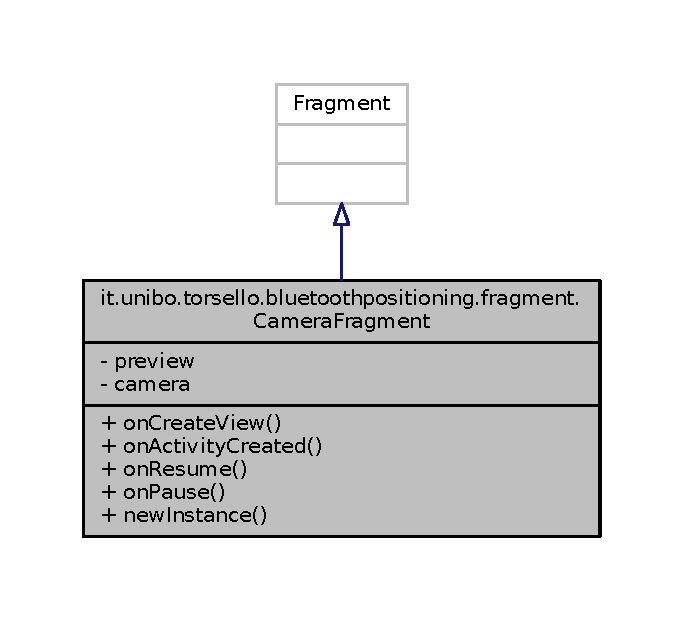
\includegraphics[width=328pt]{classit_1_1unibo_1_1torsello_1_1bluetoothpositioning_1_1fragment_1_1CameraFragment__inherit__graph}
\end{center}
\end{figure}


Diagramma di collaborazione per it.\+unibo.\+torsello.\+bluetoothpositioning.\+fragment.\+Camera\+Fragment\+:
\nopagebreak
\begin{figure}[H]
\begin{center}
\leavevmode
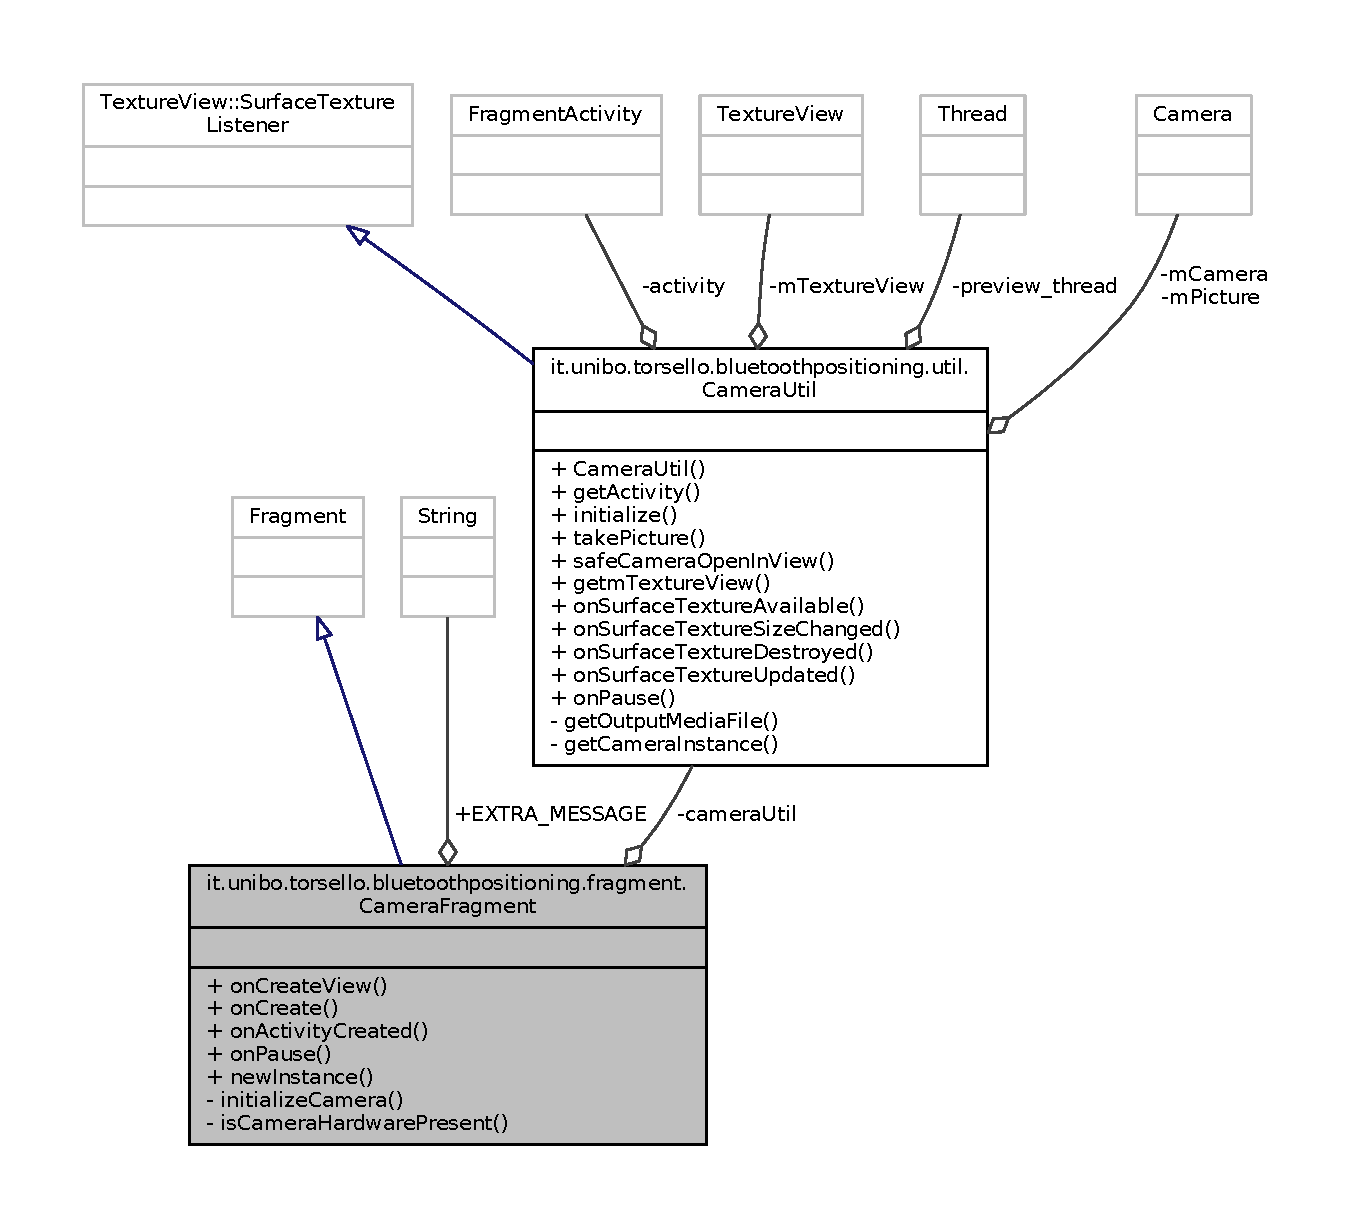
\includegraphics[width=350pt]{classit_1_1unibo_1_1torsello_1_1bluetoothpositioning_1_1fragment_1_1CameraFragment__coll__graph}
\end{center}
\end{figure}
\subsubsection*{Membri pubblici}
\begin{DoxyCompactItemize}
\item 
View \hyperlink{classit_1_1unibo_1_1torsello_1_1bluetoothpositioning_1_1fragment_1_1CameraFragment_a3a80f360922bd6a8c749cda2a09c64cf_a3a80f360922bd6a8c749cda2a09c64cf}{on\+Create\+View} (Layout\+Inflater inflater, View\+Group container, Bundle saved\+Instance\+State)
\item 
void \hyperlink{classit_1_1unibo_1_1torsello_1_1bluetoothpositioning_1_1fragment_1_1CameraFragment_a3af6cb206d2194e7d580cf511a97d6f1_a3af6cb206d2194e7d580cf511a97d6f1}{on\+Activity\+Created} (@Nullable Bundle saved\+Instance\+State)
\item 
void \hyperlink{classit_1_1unibo_1_1torsello_1_1bluetoothpositioning_1_1fragment_1_1CameraFragment_a8981ef6a92682639b28336a018bf1475_a8981ef6a92682639b28336a018bf1475}{on\+Resume} ()
\item 
void \hyperlink{classit_1_1unibo_1_1torsello_1_1bluetoothpositioning_1_1fragment_1_1CameraFragment_a3fb58eb9f1f5a3e516b9b21aa3e1e43d_a3fb58eb9f1f5a3e516b9b21aa3e1e43d}{on\+Pause} ()
\end{DoxyCompactItemize}
\subsubsection*{Membri pubblici statici}
\begin{DoxyCompactItemize}
\item 
static \hyperlink{classit_1_1unibo_1_1torsello_1_1bluetoothpositioning_1_1fragment_1_1CameraFragment}{Camera\+Fragment} \hyperlink{classit_1_1unibo_1_1torsello_1_1bluetoothpositioning_1_1fragment_1_1CameraFragment_a06506c839e3206fbe082ab705cb627b5_a06506c839e3206fbe082ab705cb627b5}{new\+Instance} ()
\end{DoxyCompactItemize}
\subsubsection*{Attributi con visibilità di package}
\begin{DoxyCompactItemize}
\item 
\hyperlink{classit_1_1unibo_1_1torsello_1_1bluetoothpositioning_1_1util_1_1CameraPreviewUtil}{Camera\+Preview\+Util} \hyperlink{classit_1_1unibo_1_1torsello_1_1bluetoothpositioning_1_1fragment_1_1CameraFragment_af14f8f1e4107c9a9063cf70d1fbb5bb5_af14f8f1e4107c9a9063cf70d1fbb5bb5}{preview}
\item 
Camera \hyperlink{classit_1_1unibo_1_1torsello_1_1bluetoothpositioning_1_1fragment_1_1CameraFragment_a70e1c67d2b127530751de08cb289b4c3_a70e1c67d2b127530751de08cb289b4c3}{camera}
\end{DoxyCompactItemize}


\subsubsection{Descrizione dettagliata}
Created by Federico Torsello. \href{mailto:federico.torsello@studio.unibo.it}{\tt federico.\+torsello@studio.\+unibo.\+it} 

\subsubsection{Documentazione delle funzioni membro}
\hypertarget{classit_1_1unibo_1_1torsello_1_1bluetoothpositioning_1_1fragment_1_1CameraFragment_a06506c839e3206fbe082ab705cb627b5_a06506c839e3206fbe082ab705cb627b5}{}\label{classit_1_1unibo_1_1torsello_1_1bluetoothpositioning_1_1fragment_1_1CameraFragment_a06506c839e3206fbe082ab705cb627b5_a06506c839e3206fbe082ab705cb627b5} 
\index{it\+::unibo\+::torsello\+::bluetoothpositioning\+::fragment\+::\+Camera\+Fragment@{it\+::unibo\+::torsello\+::bluetoothpositioning\+::fragment\+::\+Camera\+Fragment}!new\+Instance@{new\+Instance}}
\index{new\+Instance@{new\+Instance}!it\+::unibo\+::torsello\+::bluetoothpositioning\+::fragment\+::\+Camera\+Fragment@{it\+::unibo\+::torsello\+::bluetoothpositioning\+::fragment\+::\+Camera\+Fragment}}
\paragraph{\texorpdfstring{new\+Instance()}{newInstance()}}
{\footnotesize\ttfamily static \hyperlink{classit_1_1unibo_1_1torsello_1_1bluetoothpositioning_1_1fragment_1_1CameraFragment}{Camera\+Fragment} it.\+unibo.\+torsello.\+bluetoothpositioning.\+fragment.\+Camera\+Fragment.\+new\+Instance (\begin{DoxyParamCaption}{ }\end{DoxyParamCaption})\hspace{0.3cm}{\ttfamily [static]}}


\begin{DoxyCode}
25                                                \{
26         \textcolor{keywordflow}{return} \textcolor{keyword}{new} CameraFragment();
27     \}
\end{DoxyCode}
\hypertarget{classit_1_1unibo_1_1torsello_1_1bluetoothpositioning_1_1fragment_1_1CameraFragment_a3af6cb206d2194e7d580cf511a97d6f1_a3af6cb206d2194e7d580cf511a97d6f1}{}\label{classit_1_1unibo_1_1torsello_1_1bluetoothpositioning_1_1fragment_1_1CameraFragment_a3af6cb206d2194e7d580cf511a97d6f1_a3af6cb206d2194e7d580cf511a97d6f1} 
\index{it\+::unibo\+::torsello\+::bluetoothpositioning\+::fragment\+::\+Camera\+Fragment@{it\+::unibo\+::torsello\+::bluetoothpositioning\+::fragment\+::\+Camera\+Fragment}!on\+Activity\+Created@{on\+Activity\+Created}}
\index{on\+Activity\+Created@{on\+Activity\+Created}!it\+::unibo\+::torsello\+::bluetoothpositioning\+::fragment\+::\+Camera\+Fragment@{it\+::unibo\+::torsello\+::bluetoothpositioning\+::fragment\+::\+Camera\+Fragment}}
\paragraph{\texorpdfstring{on\+Activity\+Created()}{onActivityCreated()}}
{\footnotesize\ttfamily void it.\+unibo.\+torsello.\+bluetoothpositioning.\+fragment.\+Camera\+Fragment.\+on\+Activity\+Created (\begin{DoxyParamCaption}\item[{@Nullable Bundle}]{saved\+Instance\+State }\end{DoxyParamCaption})}


\begin{DoxyCode}
70                                                                        \{
71         super.onActivityCreated(savedInstanceState);
72 
73         getActivity().findViewById(R.id.fab\_camera).setOnClickListener(\textcolor{keyword}{new} View.OnClickListener() \{
74             @Override
75             \textcolor{keyword}{public} \textcolor{keywordtype}{void} onClick(View v) \{
76                 \hyperlink{classit_1_1unibo_1_1torsello_1_1bluetoothpositioning_1_1fragment_1_1CameraFragment_af14f8f1e4107c9a9063cf70d1fbb5bb5_af14f8f1e4107c9a9063cf70d1fbb5bb5}{preview}.\hyperlink{classit_1_1unibo_1_1torsello_1_1bluetoothpositioning_1_1util_1_1CameraPreviewUtil_a4f4ca8b7292c4e410f1f5aca3a53423a_a4f4ca8b7292c4e410f1f5aca3a53423a}{takePicture}();
77             \}
78         \});
79 
80     \}
\end{DoxyCode}
\hypertarget{classit_1_1unibo_1_1torsello_1_1bluetoothpositioning_1_1fragment_1_1CameraFragment_a3a80f360922bd6a8c749cda2a09c64cf_a3a80f360922bd6a8c749cda2a09c64cf}{}\label{classit_1_1unibo_1_1torsello_1_1bluetoothpositioning_1_1fragment_1_1CameraFragment_a3a80f360922bd6a8c749cda2a09c64cf_a3a80f360922bd6a8c749cda2a09c64cf} 
\index{it\+::unibo\+::torsello\+::bluetoothpositioning\+::fragment\+::\+Camera\+Fragment@{it\+::unibo\+::torsello\+::bluetoothpositioning\+::fragment\+::\+Camera\+Fragment}!on\+Create\+View@{on\+Create\+View}}
\index{on\+Create\+View@{on\+Create\+View}!it\+::unibo\+::torsello\+::bluetoothpositioning\+::fragment\+::\+Camera\+Fragment@{it\+::unibo\+::torsello\+::bluetoothpositioning\+::fragment\+::\+Camera\+Fragment}}
\paragraph{\texorpdfstring{on\+Create\+View()}{onCreateView()}}
{\footnotesize\ttfamily View it.\+unibo.\+torsello.\+bluetoothpositioning.\+fragment.\+Camera\+Fragment.\+on\+Create\+View (\begin{DoxyParamCaption}\item[{Layout\+Inflater}]{inflater,  }\item[{View\+Group}]{container,  }\item[{Bundle}]{saved\+Instance\+State }\end{DoxyParamCaption})}


\begin{DoxyCode}
30                                                                                                       \{
31 
32         View root = inflater.inflate(R.layout.fragment\_camera, container, \textcolor{keyword}{false});
33         \hyperlink{classit_1_1unibo_1_1torsello_1_1bluetoothpositioning_1_1fragment_1_1CameraFragment_af14f8f1e4107c9a9063cf70d1fbb5bb5_af14f8f1e4107c9a9063cf70d1fbb5bb5}{preview} = \textcolor{keyword}{new} CameraPreviewUtil(getContext(), (SurfaceView) root.findViewById(R.id.
      surfaceView));
34         ((FrameLayout) root.findViewById(R.id.layout)).addView(\hyperlink{classit_1_1unibo_1_1torsello_1_1bluetoothpositioning_1_1fragment_1_1CameraFragment_af14f8f1e4107c9a9063cf70d1fbb5bb5_af14f8f1e4107c9a9063cf70d1fbb5bb5}{preview});
35         \hyperlink{classit_1_1unibo_1_1torsello_1_1bluetoothpositioning_1_1fragment_1_1CameraFragment_af14f8f1e4107c9a9063cf70d1fbb5bb5_af14f8f1e4107c9a9063cf70d1fbb5bb5}{preview}.setKeepScreenOn(\textcolor{keyword}{true});
36         \hyperlink{classit_1_1unibo_1_1torsello_1_1bluetoothpositioning_1_1fragment_1_1CameraFragment_af14f8f1e4107c9a9063cf70d1fbb5bb5_af14f8f1e4107c9a9063cf70d1fbb5bb5}{preview}.setOnClickListener(\textcolor{keyword}{new} OnClickListener() \{
37 
38             @Override
39             \textcolor{keyword}{public} \textcolor{keywordtype}{void} onClick(View arg0) \{
40 \textcolor{comment}{//                preview.takePicture();}
41                 \hyperlink{classit_1_1unibo_1_1torsello_1_1bluetoothpositioning_1_1fragment_1_1CameraFragment_a70e1c67d2b127530751de08cb289b4c3_a70e1c67d2b127530751de08cb289b4c3}{camera}.autoFocus(\textcolor{keyword}{new} Camera.AutoFocusCallback() \{
42                     @Override
43                     \textcolor{keyword}{public} \textcolor{keywordtype}{void} onAutoFocus(\textcolor{keywordtype}{boolean} success, Camera arg1) \{
44 \textcolor{comment}{//                        if (success) \{}
45 \textcolor{comment}{//                            preview.takePicture();}
46 \textcolor{comment}{//                        \}}
47                     \}
48                 \});
49             \}
50         \});
51         \hyperlink{classit_1_1unibo_1_1torsello_1_1bluetoothpositioning_1_1fragment_1_1CameraFragment_af14f8f1e4107c9a9063cf70d1fbb5bb5_af14f8f1e4107c9a9063cf70d1fbb5bb5}{preview}.setOnLongClickListener(\textcolor{keyword}{new} View.OnLongClickListener() \{
52             @Override
53             \textcolor{keyword}{public} \textcolor{keywordtype}{boolean} onLongClick(View arg0) \{
54 
55                 \hyperlink{classit_1_1unibo_1_1torsello_1_1bluetoothpositioning_1_1fragment_1_1CameraFragment_a70e1c67d2b127530751de08cb289b4c3_a70e1c67d2b127530751de08cb289b4c3}{camera}.autoFocus(\textcolor{keyword}{new} Camera.AutoFocusCallback() \{
56                     @Override
57                     \textcolor{keyword}{public} \textcolor{keywordtype}{void} onAutoFocus(\textcolor{keywordtype}{boolean} success, Camera arg1) \{
58 \textcolor{comment}{//                        if (success) \{}
59 \textcolor{comment}{//                            preview.takePicture();}
60 \textcolor{comment}{//                        \}}
61                     \}
62                 \});
63                 \textcolor{keywordflow}{return} \textcolor{keyword}{true};
64             \}
65         \});
66         \textcolor{keywordflow}{return} root;
67     \}
\end{DoxyCode}
\hypertarget{classit_1_1unibo_1_1torsello_1_1bluetoothpositioning_1_1fragment_1_1CameraFragment_a3fb58eb9f1f5a3e516b9b21aa3e1e43d_a3fb58eb9f1f5a3e516b9b21aa3e1e43d}{}\label{classit_1_1unibo_1_1torsello_1_1bluetoothpositioning_1_1fragment_1_1CameraFragment_a3fb58eb9f1f5a3e516b9b21aa3e1e43d_a3fb58eb9f1f5a3e516b9b21aa3e1e43d} 
\index{it\+::unibo\+::torsello\+::bluetoothpositioning\+::fragment\+::\+Camera\+Fragment@{it\+::unibo\+::torsello\+::bluetoothpositioning\+::fragment\+::\+Camera\+Fragment}!on\+Pause@{on\+Pause}}
\index{on\+Pause@{on\+Pause}!it\+::unibo\+::torsello\+::bluetoothpositioning\+::fragment\+::\+Camera\+Fragment@{it\+::unibo\+::torsello\+::bluetoothpositioning\+::fragment\+::\+Camera\+Fragment}}
\paragraph{\texorpdfstring{on\+Pause()}{onPause()}}
{\footnotesize\ttfamily void it.\+unibo.\+torsello.\+bluetoothpositioning.\+fragment.\+Camera\+Fragment.\+on\+Pause (\begin{DoxyParamCaption}{ }\end{DoxyParamCaption})}


\begin{DoxyCode}
90                           \{
91         \hyperlink{classit_1_1unibo_1_1torsello_1_1bluetoothpositioning_1_1fragment_1_1CameraFragment_af14f8f1e4107c9a9063cf70d1fbb5bb5_af14f8f1e4107c9a9063cf70d1fbb5bb5}{preview}.\hyperlink{classit_1_1unibo_1_1torsello_1_1bluetoothpositioning_1_1util_1_1CameraPreviewUtil_a69da006b39dff168a1cd185c5aa886f8_a69da006b39dff168a1cd185c5aa886f8}{onPause}();
92         super.onPause();
93     \}
\end{DoxyCode}
\hypertarget{classit_1_1unibo_1_1torsello_1_1bluetoothpositioning_1_1fragment_1_1CameraFragment_a8981ef6a92682639b28336a018bf1475_a8981ef6a92682639b28336a018bf1475}{}\label{classit_1_1unibo_1_1torsello_1_1bluetoothpositioning_1_1fragment_1_1CameraFragment_a8981ef6a92682639b28336a018bf1475_a8981ef6a92682639b28336a018bf1475} 
\index{it\+::unibo\+::torsello\+::bluetoothpositioning\+::fragment\+::\+Camera\+Fragment@{it\+::unibo\+::torsello\+::bluetoothpositioning\+::fragment\+::\+Camera\+Fragment}!on\+Resume@{on\+Resume}}
\index{on\+Resume@{on\+Resume}!it\+::unibo\+::torsello\+::bluetoothpositioning\+::fragment\+::\+Camera\+Fragment@{it\+::unibo\+::torsello\+::bluetoothpositioning\+::fragment\+::\+Camera\+Fragment}}
\paragraph{\texorpdfstring{on\+Resume()}{onResume()}}
{\footnotesize\ttfamily void it.\+unibo.\+torsello.\+bluetoothpositioning.\+fragment.\+Camera\+Fragment.\+on\+Resume (\begin{DoxyParamCaption}{ }\end{DoxyParamCaption})}


\begin{DoxyCode}
83                            \{
84         super.onResume();
85         \hyperlink{classit_1_1unibo_1_1torsello_1_1bluetoothpositioning_1_1fragment_1_1CameraFragment_af14f8f1e4107c9a9063cf70d1fbb5bb5_af14f8f1e4107c9a9063cf70d1fbb5bb5}{preview}.\hyperlink{classit_1_1unibo_1_1torsello_1_1bluetoothpositioning_1_1util_1_1CameraPreviewUtil_acc49f348e381371fcad9d428ea4a15ca_acc49f348e381371fcad9d428ea4a15ca}{setCamera}(getActivity());
86         \hyperlink{classit_1_1unibo_1_1torsello_1_1bluetoothpositioning_1_1fragment_1_1CameraFragment_a70e1c67d2b127530751de08cb289b4c3_a70e1c67d2b127530751de08cb289b4c3}{camera} = \hyperlink{classit_1_1unibo_1_1torsello_1_1bluetoothpositioning_1_1fragment_1_1CameraFragment_af14f8f1e4107c9a9063cf70d1fbb5bb5_af14f8f1e4107c9a9063cf70d1fbb5bb5}{preview}.\hyperlink{classit_1_1unibo_1_1torsello_1_1bluetoothpositioning_1_1util_1_1CameraPreviewUtil_a24b83bd2a152f8f12824ccf190a90369_a24b83bd2a152f8f12824ccf190a90369}{getCamera}();
87     \}
\end{DoxyCode}


\subsubsection{Documentazione dei membri dato}
\hypertarget{classit_1_1unibo_1_1torsello_1_1bluetoothpositioning_1_1fragment_1_1CameraFragment_a70e1c67d2b127530751de08cb289b4c3_a70e1c67d2b127530751de08cb289b4c3}{}\label{classit_1_1unibo_1_1torsello_1_1bluetoothpositioning_1_1fragment_1_1CameraFragment_a70e1c67d2b127530751de08cb289b4c3_a70e1c67d2b127530751de08cb289b4c3} 
\index{it\+::unibo\+::torsello\+::bluetoothpositioning\+::fragment\+::\+Camera\+Fragment@{it\+::unibo\+::torsello\+::bluetoothpositioning\+::fragment\+::\+Camera\+Fragment}!camera@{camera}}
\index{camera@{camera}!it\+::unibo\+::torsello\+::bluetoothpositioning\+::fragment\+::\+Camera\+Fragment@{it\+::unibo\+::torsello\+::bluetoothpositioning\+::fragment\+::\+Camera\+Fragment}}
\paragraph{\texorpdfstring{camera}{camera}}
{\footnotesize\ttfamily Camera it.\+unibo.\+torsello.\+bluetoothpositioning.\+fragment.\+Camera\+Fragment.\+camera\hspace{0.3cm}{\ttfamily [package]}}

\hypertarget{classit_1_1unibo_1_1torsello_1_1bluetoothpositioning_1_1fragment_1_1CameraFragment_af14f8f1e4107c9a9063cf70d1fbb5bb5_af14f8f1e4107c9a9063cf70d1fbb5bb5}{}\label{classit_1_1unibo_1_1torsello_1_1bluetoothpositioning_1_1fragment_1_1CameraFragment_af14f8f1e4107c9a9063cf70d1fbb5bb5_af14f8f1e4107c9a9063cf70d1fbb5bb5} 
\index{it\+::unibo\+::torsello\+::bluetoothpositioning\+::fragment\+::\+Camera\+Fragment@{it\+::unibo\+::torsello\+::bluetoothpositioning\+::fragment\+::\+Camera\+Fragment}!preview@{preview}}
\index{preview@{preview}!it\+::unibo\+::torsello\+::bluetoothpositioning\+::fragment\+::\+Camera\+Fragment@{it\+::unibo\+::torsello\+::bluetoothpositioning\+::fragment\+::\+Camera\+Fragment}}
\paragraph{\texorpdfstring{preview}{preview}}
{\footnotesize\ttfamily \hyperlink{classit_1_1unibo_1_1torsello_1_1bluetoothpositioning_1_1util_1_1CameraPreviewUtil}{Camera\+Preview\+Util} it.\+unibo.\+torsello.\+bluetoothpositioning.\+fragment.\+Camera\+Fragment.\+preview\hspace{0.3cm}{\ttfamily [package]}}



La documentazione per questa classe è stata generata a partire dal seguente file\+:\begin{DoxyCompactItemize}
\item 
\hyperlink{CameraFragment_8java}{Camera\+Fragment.\+java}\end{DoxyCompactItemize}

\hypertarget{classit_1_1unibo_1_1torsello_1_1bluetoothpositioning_1_1util_1_1CameraPreviewUtil}{}\subsection{Riferimenti per la classe it.\+unibo.\+torsello.\+bluetoothpositioning.\+util.\+Camera\+Preview\+Util}
\label{classit_1_1unibo_1_1torsello_1_1bluetoothpositioning_1_1util_1_1CameraPreviewUtil}\index{it.\+unibo.\+torsello.\+bluetoothpositioning.\+util.\+Camera\+Preview\+Util@{it.\+unibo.\+torsello.\+bluetoothpositioning.\+util.\+Camera\+Preview\+Util}}


Diagramma delle classi per it.\+unibo.\+torsello.\+bluetoothpositioning.\+util.\+Camera\+Preview\+Util
\nopagebreak
\begin{figure}[H]
\begin{center}
\leavevmode
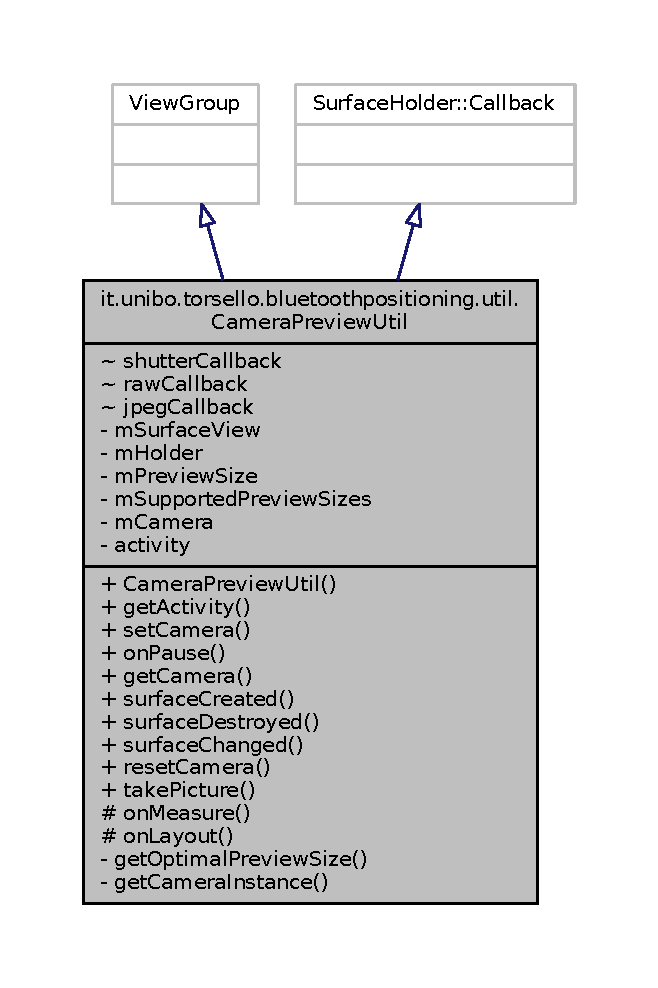
\includegraphics[width=316pt]{classit_1_1unibo_1_1torsello_1_1bluetoothpositioning_1_1util_1_1CameraPreviewUtil__inherit__graph}
\end{center}
\end{figure}


Diagramma di collaborazione per it.\+unibo.\+torsello.\+bluetoothpositioning.\+util.\+Camera\+Preview\+Util\+:
\nopagebreak
\begin{figure}[H]
\begin{center}
\leavevmode
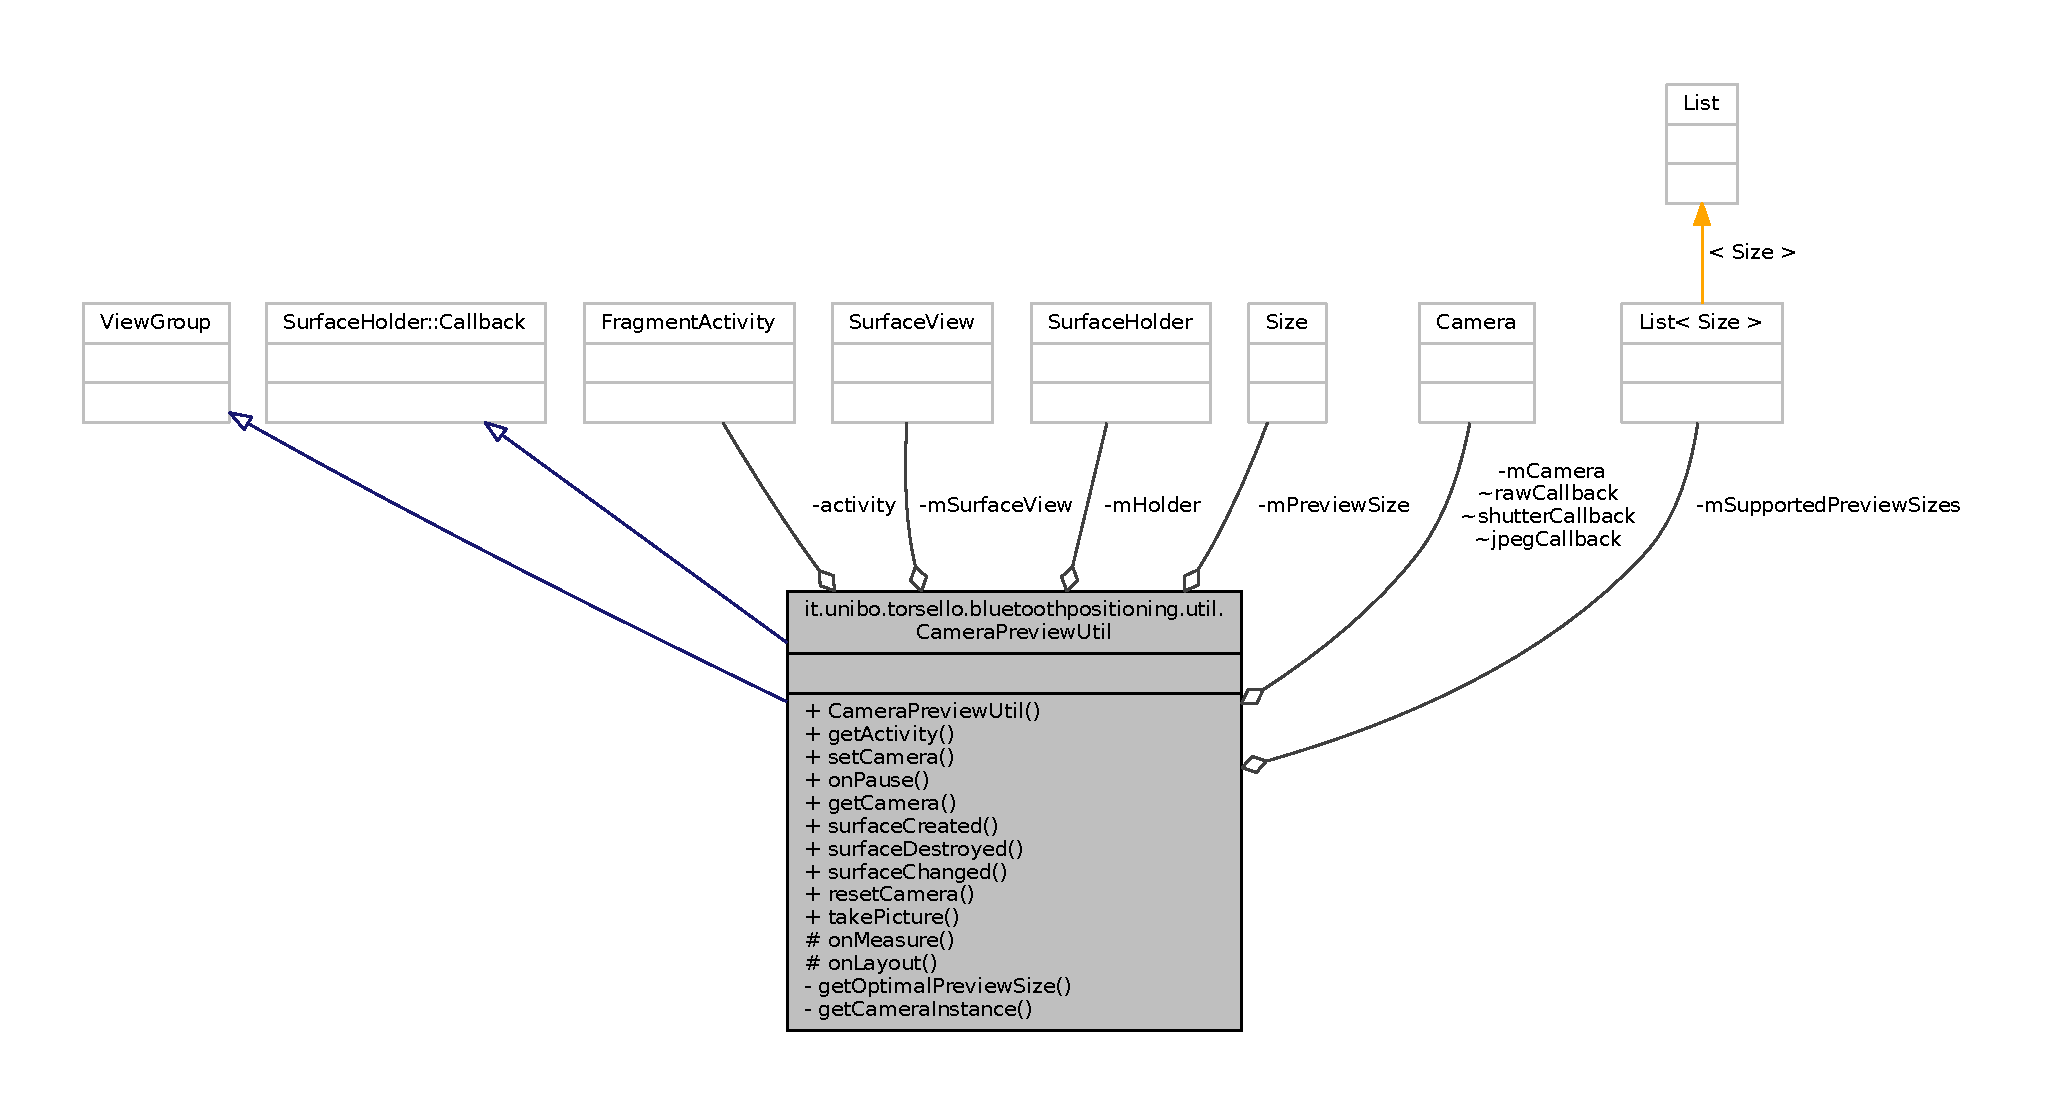
\includegraphics[width=350pt]{classit_1_1unibo_1_1torsello_1_1bluetoothpositioning_1_1util_1_1CameraPreviewUtil__coll__graph}
\end{center}
\end{figure}
\subsubsection*{Membri pubblici}
\begin{DoxyCompactItemize}
\item 
\hyperlink{classit_1_1unibo_1_1torsello_1_1bluetoothpositioning_1_1util_1_1CameraPreviewUtil_aa0b929d195ddb472745e4c26d576758e_aa0b929d195ddb472745e4c26d576758e}{Camera\+Preview\+Util} (Context context, Surface\+View sv)
\item 
Fragment\+Activity \hyperlink{classit_1_1unibo_1_1torsello_1_1bluetoothpositioning_1_1util_1_1CameraPreviewUtil_a3a4253aa9b4df3659a6f7bb80be84256_a3a4253aa9b4df3659a6f7bb80be84256}{get\+Activity} ()
\item 
void \hyperlink{classit_1_1unibo_1_1torsello_1_1bluetoothpositioning_1_1util_1_1CameraPreviewUtil_acc49f348e381371fcad9d428ea4a15ca_acc49f348e381371fcad9d428ea4a15ca}{set\+Camera} (Fragment\+Activity fragment\+Activity)
\item 
void \hyperlink{classit_1_1unibo_1_1torsello_1_1bluetoothpositioning_1_1util_1_1CameraPreviewUtil_a69da006b39dff168a1cd185c5aa886f8_a69da006b39dff168a1cd185c5aa886f8}{on\+Pause} ()
\item 
Camera \hyperlink{classit_1_1unibo_1_1torsello_1_1bluetoothpositioning_1_1util_1_1CameraPreviewUtil_a24b83bd2a152f8f12824ccf190a90369_a24b83bd2a152f8f12824ccf190a90369}{get\+Camera} ()
\item 
void \hyperlink{classit_1_1unibo_1_1torsello_1_1bluetoothpositioning_1_1util_1_1CameraPreviewUtil_a88d3e6e94bb5cb4c73e8155e009b6270_a88d3e6e94bb5cb4c73e8155e009b6270}{surface\+Created} (Surface\+Holder holder)
\item 
void \hyperlink{classit_1_1unibo_1_1torsello_1_1bluetoothpositioning_1_1util_1_1CameraPreviewUtil_ab5010e060d99e2808402b40555ba7c1a_ab5010e060d99e2808402b40555ba7c1a}{surface\+Destroyed} (Surface\+Holder holder)
\item 
void \hyperlink{classit_1_1unibo_1_1torsello_1_1bluetoothpositioning_1_1util_1_1CameraPreviewUtil_a1b606e27ab2a6587818cc011dd5ff7f6_a1b606e27ab2a6587818cc011dd5ff7f6}{surface\+Changed} (Surface\+Holder holder, int format, int w, int h)
\item 
void \hyperlink{classit_1_1unibo_1_1torsello_1_1bluetoothpositioning_1_1util_1_1CameraPreviewUtil_a5240e32d2ccac682cf80c639accea5da_a5240e32d2ccac682cf80c639accea5da}{reset\+Camera} ()
\item 
void \hyperlink{classit_1_1unibo_1_1torsello_1_1bluetoothpositioning_1_1util_1_1CameraPreviewUtil_a4f4ca8b7292c4e410f1f5aca3a53423a_a4f4ca8b7292c4e410f1f5aca3a53423a}{take\+Picture} ()
\end{DoxyCompactItemize}
\subsubsection*{Membri protetti}
\begin{DoxyCompactItemize}
\item 
void \hyperlink{classit_1_1unibo_1_1torsello_1_1bluetoothpositioning_1_1util_1_1CameraPreviewUtil_ad173ec9f318b978c9304482d432c8b21_ad173ec9f318b978c9304482d432c8b21}{on\+Measure} (int width\+Measure\+Spec, int height\+Measure\+Spec)
\item 
void \hyperlink{classit_1_1unibo_1_1torsello_1_1bluetoothpositioning_1_1util_1_1CameraPreviewUtil_a3b2897b27ca62e95df13f63d8d09e036_a3b2897b27ca62e95df13f63d8d09e036}{on\+Layout} (boolean changed, int l, int t, int r, int b)
\end{DoxyCompactItemize}
\subsubsection*{Attributi con visibilità di package}
\begin{DoxyCompactItemize}
\item 
Camera.\+Shutter\+Callback \hyperlink{classit_1_1unibo_1_1torsello_1_1bluetoothpositioning_1_1util_1_1CameraPreviewUtil_a146053288e01aa0d0ad482050182a1a4_a146053288e01aa0d0ad482050182a1a4}{shutter\+Callback}
\item 
Camera.\+Picture\+Callback \hyperlink{classit_1_1unibo_1_1torsello_1_1bluetoothpositioning_1_1util_1_1CameraPreviewUtil_a64b624b7bd81370fb4e80d3cb9226635_a64b624b7bd81370fb4e80d3cb9226635}{raw\+Callback}
\item 
Camera.\+Picture\+Callback \hyperlink{classit_1_1unibo_1_1torsello_1_1bluetoothpositioning_1_1util_1_1CameraPreviewUtil_aff50f9e425599097ed50d6d8341ed891_aff50f9e425599097ed50d6d8341ed891}{jpeg\+Callback}
\end{DoxyCompactItemize}
\subsubsection*{Membri privati}
\begin{DoxyCompactItemize}
\item 
Size \hyperlink{classit_1_1unibo_1_1torsello_1_1bluetoothpositioning_1_1util_1_1CameraPreviewUtil_ac7a729182a7e912d771f587f89a2ce03_ac7a729182a7e912d771f587f89a2ce03}{get\+Optimal\+Preview\+Size} (List$<$ Size $>$ sizes, int w, int h)
\end{DoxyCompactItemize}
\subsubsection*{Membri privati statici}
\begin{DoxyCompactItemize}
\item 
static Camera \hyperlink{classit_1_1unibo_1_1torsello_1_1bluetoothpositioning_1_1util_1_1CameraPreviewUtil_a7bfe209167872194f9237f51ece4cbf7_a7bfe209167872194f9237f51ece4cbf7}{get\+Camera\+Instance} ()
\end{DoxyCompactItemize}
\subsubsection*{Attributi privati}
\begin{DoxyCompactItemize}
\item 
Surface\+View \hyperlink{classit_1_1unibo_1_1torsello_1_1bluetoothpositioning_1_1util_1_1CameraPreviewUtil_a41e834d4998c7df0228da7b4b517f9b0_a41e834d4998c7df0228da7b4b517f9b0}{m\+Surface\+View}
\item 
Surface\+Holder \hyperlink{classit_1_1unibo_1_1torsello_1_1bluetoothpositioning_1_1util_1_1CameraPreviewUtil_ad2698fd1398d4a6491b1e0b071a956db_ad2698fd1398d4a6491b1e0b071a956db}{m\+Holder}
\item 
Size \hyperlink{classit_1_1unibo_1_1torsello_1_1bluetoothpositioning_1_1util_1_1CameraPreviewUtil_a48550a4bc1d9358ae5de55f1109a2966_a48550a4bc1d9358ae5de55f1109a2966}{m\+Preview\+Size}
\item 
List$<$ Size $>$ \hyperlink{classit_1_1unibo_1_1torsello_1_1bluetoothpositioning_1_1util_1_1CameraPreviewUtil_a4aeb809017d527738a2b2be1ebe2cb39_a4aeb809017d527738a2b2be1ebe2cb39}{m\+Supported\+Preview\+Sizes}
\item 
Camera \hyperlink{classit_1_1unibo_1_1torsello_1_1bluetoothpositioning_1_1util_1_1CameraPreviewUtil_a7ee402da8ec64412f9a68e68b4025eea_a7ee402da8ec64412f9a68e68b4025eea}{m\+Camera}
\item 
Fragment\+Activity \hyperlink{classit_1_1unibo_1_1torsello_1_1bluetoothpositioning_1_1util_1_1CameraPreviewUtil_ab3f45258d2ab144fd4be5db55d278c42_ab3f45258d2ab144fd4be5db55d278c42}{activity}
\end{DoxyCompactItemize}


\subsubsection{Descrizione dettagliata}
Created by Federico Torsello. \href{mailto:federico.torsello@studio.unibo.it}{\tt federico.\+torsello@studio.\+unibo.\+it} 

\subsubsection{Documentazione dei costruttori e dei distruttori}
\hypertarget{classit_1_1unibo_1_1torsello_1_1bluetoothpositioning_1_1util_1_1CameraPreviewUtil_aa0b929d195ddb472745e4c26d576758e_aa0b929d195ddb472745e4c26d576758e}{}\label{classit_1_1unibo_1_1torsello_1_1bluetoothpositioning_1_1util_1_1CameraPreviewUtil_aa0b929d195ddb472745e4c26d576758e_aa0b929d195ddb472745e4c26d576758e} 
\index{it\+::unibo\+::torsello\+::bluetoothpositioning\+::util\+::\+Camera\+Preview\+Util@{it\+::unibo\+::torsello\+::bluetoothpositioning\+::util\+::\+Camera\+Preview\+Util}!Camera\+Preview\+Util@{Camera\+Preview\+Util}}
\index{Camera\+Preview\+Util@{Camera\+Preview\+Util}!it\+::unibo\+::torsello\+::bluetoothpositioning\+::util\+::\+Camera\+Preview\+Util@{it\+::unibo\+::torsello\+::bluetoothpositioning\+::util\+::\+Camera\+Preview\+Util}}
\paragraph{\texorpdfstring{Camera\+Preview\+Util()}{CameraPreviewUtil()}}
{\footnotesize\ttfamily it.\+unibo.\+torsello.\+bluetoothpositioning.\+util.\+Camera\+Preview\+Util.\+Camera\+Preview\+Util (\begin{DoxyParamCaption}\item[{Context}]{context,  }\item[{Surface\+View}]{sv }\end{DoxyParamCaption})}


\begin{DoxyCode}
32                                                               \{
33         super(context);
34         \hyperlink{classit_1_1unibo_1_1torsello_1_1bluetoothpositioning_1_1util_1_1CameraPreviewUtil_a41e834d4998c7df0228da7b4b517f9b0_a41e834d4998c7df0228da7b4b517f9b0}{mSurfaceView} = sv;
35 
36         \hyperlink{classit_1_1unibo_1_1torsello_1_1bluetoothpositioning_1_1util_1_1CameraPreviewUtil_ad2698fd1398d4a6491b1e0b071a956db_ad2698fd1398d4a6491b1e0b071a956db}{mHolder} = \hyperlink{classit_1_1unibo_1_1torsello_1_1bluetoothpositioning_1_1util_1_1CameraPreviewUtil_a41e834d4998c7df0228da7b4b517f9b0_a41e834d4998c7df0228da7b4b517f9b0}{mSurfaceView}.getHolder();
37         \hyperlink{classit_1_1unibo_1_1torsello_1_1bluetoothpositioning_1_1util_1_1CameraPreviewUtil_ad2698fd1398d4a6491b1e0b071a956db_ad2698fd1398d4a6491b1e0b071a956db}{mHolder}.addCallback(\textcolor{keyword}{this});
38         \hyperlink{classit_1_1unibo_1_1torsello_1_1bluetoothpositioning_1_1util_1_1CameraPreviewUtil_ad2698fd1398d4a6491b1e0b071a956db_ad2698fd1398d4a6491b1e0b071a956db}{mHolder}.setType(SurfaceHolder.SURFACE\_TYPE\_PUSH\_BUFFERS);
39     \}
\end{DoxyCode}


\subsubsection{Documentazione delle funzioni membro}
\hypertarget{classit_1_1unibo_1_1torsello_1_1bluetoothpositioning_1_1util_1_1CameraPreviewUtil_a3a4253aa9b4df3659a6f7bb80be84256_a3a4253aa9b4df3659a6f7bb80be84256}{}\label{classit_1_1unibo_1_1torsello_1_1bluetoothpositioning_1_1util_1_1CameraPreviewUtil_a3a4253aa9b4df3659a6f7bb80be84256_a3a4253aa9b4df3659a6f7bb80be84256} 
\index{it\+::unibo\+::torsello\+::bluetoothpositioning\+::util\+::\+Camera\+Preview\+Util@{it\+::unibo\+::torsello\+::bluetoothpositioning\+::util\+::\+Camera\+Preview\+Util}!get\+Activity@{get\+Activity}}
\index{get\+Activity@{get\+Activity}!it\+::unibo\+::torsello\+::bluetoothpositioning\+::util\+::\+Camera\+Preview\+Util@{it\+::unibo\+::torsello\+::bluetoothpositioning\+::util\+::\+Camera\+Preview\+Util}}
\paragraph{\texorpdfstring{get\+Activity()}{getActivity()}}
{\footnotesize\ttfamily Fragment\+Activity it.\+unibo.\+torsello.\+bluetoothpositioning.\+util.\+Camera\+Preview\+Util.\+get\+Activity (\begin{DoxyParamCaption}{ }\end{DoxyParamCaption})}


\begin{DoxyCode}
41                                           \{
42         \textcolor{keywordflow}{return} \hyperlink{classit_1_1unibo_1_1torsello_1_1bluetoothpositioning_1_1util_1_1CameraPreviewUtil_ab3f45258d2ab144fd4be5db55d278c42_ab3f45258d2ab144fd4be5db55d278c42}{activity};
43     \}
\end{DoxyCode}
\hypertarget{classit_1_1unibo_1_1torsello_1_1bluetoothpositioning_1_1util_1_1CameraPreviewUtil_a24b83bd2a152f8f12824ccf190a90369_a24b83bd2a152f8f12824ccf190a90369}{}\label{classit_1_1unibo_1_1torsello_1_1bluetoothpositioning_1_1util_1_1CameraPreviewUtil_a24b83bd2a152f8f12824ccf190a90369_a24b83bd2a152f8f12824ccf190a90369} 
\index{it\+::unibo\+::torsello\+::bluetoothpositioning\+::util\+::\+Camera\+Preview\+Util@{it\+::unibo\+::torsello\+::bluetoothpositioning\+::util\+::\+Camera\+Preview\+Util}!get\+Camera@{get\+Camera}}
\index{get\+Camera@{get\+Camera}!it\+::unibo\+::torsello\+::bluetoothpositioning\+::util\+::\+Camera\+Preview\+Util@{it\+::unibo\+::torsello\+::bluetoothpositioning\+::util\+::\+Camera\+Preview\+Util}}
\paragraph{\texorpdfstring{get\+Camera()}{getCamera()}}
{\footnotesize\ttfamily Camera it.\+unibo.\+torsello.\+bluetoothpositioning.\+util.\+Camera\+Preview\+Util.\+get\+Camera (\begin{DoxyParamCaption}{ }\end{DoxyParamCaption})}


\begin{DoxyCode}
81                               \{
82         \textcolor{keywordflow}{return} \hyperlink{classit_1_1unibo_1_1torsello_1_1bluetoothpositioning_1_1util_1_1CameraPreviewUtil_a7ee402da8ec64412f9a68e68b4025eea_a7ee402da8ec64412f9a68e68b4025eea}{mCamera};
83     \}
\end{DoxyCode}
\hypertarget{classit_1_1unibo_1_1torsello_1_1bluetoothpositioning_1_1util_1_1CameraPreviewUtil_a7bfe209167872194f9237f51ece4cbf7_a7bfe209167872194f9237f51ece4cbf7}{}\label{classit_1_1unibo_1_1torsello_1_1bluetoothpositioning_1_1util_1_1CameraPreviewUtil_a7bfe209167872194f9237f51ece4cbf7_a7bfe209167872194f9237f51ece4cbf7} 
\index{it\+::unibo\+::torsello\+::bluetoothpositioning\+::util\+::\+Camera\+Preview\+Util@{it\+::unibo\+::torsello\+::bluetoothpositioning\+::util\+::\+Camera\+Preview\+Util}!get\+Camera\+Instance@{get\+Camera\+Instance}}
\index{get\+Camera\+Instance@{get\+Camera\+Instance}!it\+::unibo\+::torsello\+::bluetoothpositioning\+::util\+::\+Camera\+Preview\+Util@{it\+::unibo\+::torsello\+::bluetoothpositioning\+::util\+::\+Camera\+Preview\+Util}}
\paragraph{\texorpdfstring{get\+Camera\+Instance()}{getCameraInstance()}}
{\footnotesize\ttfamily static Camera it.\+unibo.\+torsello.\+bluetoothpositioning.\+util.\+Camera\+Preview\+Util.\+get\+Camera\+Instance (\begin{DoxyParamCaption}{ }\end{DoxyParamCaption})\hspace{0.3cm}{\ttfamily [static]}, {\ttfamily [private]}}

A safe way to get an instance of the Camera\+Util object. 
\begin{DoxyCode}
88                                               \{
89 
90         Camera c = null;
91 
92         \textcolor{keywordflow}{try} \{
93             \textcolor{keywordtype}{int} numCams = Camera.getNumberOfCameras();
94             \textcolor{keywordflow}{if} (numCams > 0) \{
95                 c = Camera.open(0); \textcolor{comment}{// attempt to get a CameraUtil instance}
96             \}
97         \} \textcolor{keywordflow}{catch} (RuntimeException e) \{
98             \textcolor{comment}{// CameraUtil is not available (in use or does not exist)}
99             e.getStackTrace();
100         \}
101 
102         \textcolor{keywordflow}{return} c; \textcolor{comment}{// returns null if camera is unavailable}
103     \}
\end{DoxyCode}
\hypertarget{classit_1_1unibo_1_1torsello_1_1bluetoothpositioning_1_1util_1_1CameraPreviewUtil_ac7a729182a7e912d771f587f89a2ce03_ac7a729182a7e912d771f587f89a2ce03}{}\label{classit_1_1unibo_1_1torsello_1_1bluetoothpositioning_1_1util_1_1CameraPreviewUtil_ac7a729182a7e912d771f587f89a2ce03_ac7a729182a7e912d771f587f89a2ce03} 
\index{it\+::unibo\+::torsello\+::bluetoothpositioning\+::util\+::\+Camera\+Preview\+Util@{it\+::unibo\+::torsello\+::bluetoothpositioning\+::util\+::\+Camera\+Preview\+Util}!get\+Optimal\+Preview\+Size@{get\+Optimal\+Preview\+Size}}
\index{get\+Optimal\+Preview\+Size@{get\+Optimal\+Preview\+Size}!it\+::unibo\+::torsello\+::bluetoothpositioning\+::util\+::\+Camera\+Preview\+Util@{it\+::unibo\+::torsello\+::bluetoothpositioning\+::util\+::\+Camera\+Preview\+Util}}
\paragraph{\texorpdfstring{get\+Optimal\+Preview\+Size()}{getOptimalPreviewSize()}}
{\footnotesize\ttfamily Size it.\+unibo.\+torsello.\+bluetoothpositioning.\+util.\+Camera\+Preview\+Util.\+get\+Optimal\+Preview\+Size (\begin{DoxyParamCaption}\item[{List$<$ Size $>$}]{sizes,  }\item[{int}]{w,  }\item[{int}]{h }\end{DoxyParamCaption})\hspace{0.3cm}{\ttfamily [private]}}


\begin{DoxyCode}
169                                                                        \{
170         \textcolor{keyword}{final} \textcolor{keywordtype}{double} ASPECT\_TOLERANCE = 0.1;
171         \textcolor{keywordtype}{double} targetRatio = (double) w / h;
172         \textcolor{keywordflow}{if} (sizes == null) \textcolor{keywordflow}{return} null;
173 
174         Size optimalSize = null;
175         \textcolor{keywordtype}{double} minDiff = Double.MAX\_VALUE;
176 
177 \textcolor{comment}{//        int targetHeight = h;}
178 
179         \textcolor{comment}{// Try to find an size match aspect ratio and size}
180         \textcolor{keywordflow}{for} (Size size : sizes) \{
181             \textcolor{keywordtype}{double} ratio = (double) size.width / size.height;
182             if (Math.abs(ratio - targetRatio) > ASPECT\_TOLERANCE) \textcolor{keywordflow}{continue};
183             \textcolor{keywordflow}{if} (Math.abs(size.height - h) < minDiff) \{
184                 optimalSize = size;
185                 minDiff = Math.abs(size.height - h);
186             \}
187         \}
188 
189         \textcolor{comment}{// Cannot find the one match the aspect ratio, ignore the requirement}
190         \textcolor{keywordflow}{if} (optimalSize == null) \{
191             minDiff = Double.MAX\_VALUE;
192             \textcolor{keywordflow}{for} (Size size : sizes) \{
193                 \textcolor{keywordflow}{if} (Math.abs(size.height - h) < minDiff) \{
194                     optimalSize = size;
195                     minDiff = Math.abs(size.height - h);
196                 \}
197             \}
198         \}
199         \textcolor{keywordflow}{return} optimalSize;
200     \}
\end{DoxyCode}
\hypertarget{classit_1_1unibo_1_1torsello_1_1bluetoothpositioning_1_1util_1_1CameraPreviewUtil_a3b2897b27ca62e95df13f63d8d09e036_a3b2897b27ca62e95df13f63d8d09e036}{}\label{classit_1_1unibo_1_1torsello_1_1bluetoothpositioning_1_1util_1_1CameraPreviewUtil_a3b2897b27ca62e95df13f63d8d09e036_a3b2897b27ca62e95df13f63d8d09e036} 
\index{it\+::unibo\+::torsello\+::bluetoothpositioning\+::util\+::\+Camera\+Preview\+Util@{it\+::unibo\+::torsello\+::bluetoothpositioning\+::util\+::\+Camera\+Preview\+Util}!on\+Layout@{on\+Layout}}
\index{on\+Layout@{on\+Layout}!it\+::unibo\+::torsello\+::bluetoothpositioning\+::util\+::\+Camera\+Preview\+Util@{it\+::unibo\+::torsello\+::bluetoothpositioning\+::util\+::\+Camera\+Preview\+Util}}
\paragraph{\texorpdfstring{on\+Layout()}{onLayout()}}
{\footnotesize\ttfamily void it.\+unibo.\+torsello.\+bluetoothpositioning.\+util.\+Camera\+Preview\+Util.\+on\+Layout (\begin{DoxyParamCaption}\item[{boolean}]{changed,  }\item[{int}]{l,  }\item[{int}]{t,  }\item[{int}]{r,  }\item[{int}]{b }\end{DoxyParamCaption})\hspace{0.3cm}{\ttfamily [protected]}}


\begin{DoxyCode}
120                                                                          \{
121         \textcolor{keywordflow}{if} (changed && getChildCount() > 0) \{
122             \textcolor{keyword}{final} View child = getChildAt(0);
123 
124             \textcolor{keyword}{final} \textcolor{keywordtype}{int} width = r - l;
125             \textcolor{keyword}{final} \textcolor{keywordtype}{int} height = b - t;
126 
127             \textcolor{keywordtype}{int} previewWidth = width;
128             \textcolor{keywordtype}{int} previewHeight = height;
129             \textcolor{keywordflow}{if} (\hyperlink{classit_1_1unibo_1_1torsello_1_1bluetoothpositioning_1_1util_1_1CameraPreviewUtil_a48550a4bc1d9358ae5de55f1109a2966_a48550a4bc1d9358ae5de55f1109a2966}{mPreviewSize} != null) \{
130                 previewWidth = \hyperlink{classit_1_1unibo_1_1torsello_1_1bluetoothpositioning_1_1util_1_1CameraPreviewUtil_a48550a4bc1d9358ae5de55f1109a2966_a48550a4bc1d9358ae5de55f1109a2966}{mPreviewSize}.width;
131                 previewHeight = \hyperlink{classit_1_1unibo_1_1torsello_1_1bluetoothpositioning_1_1util_1_1CameraPreviewUtil_a48550a4bc1d9358ae5de55f1109a2966_a48550a4bc1d9358ae5de55f1109a2966}{mPreviewSize}.height;
132             \}
133 
134             \textcolor{comment}{// Center the child SurfaceView within the parent.}
135             \textcolor{keywordflow}{if} (width * previewHeight > height * previewWidth) \{
136                 \textcolor{keyword}{final} \textcolor{keywordtype}{int} scaledChildWidth = previewWidth * height / previewHeight;
137                 child.layout((width - scaledChildWidth) / 2, 0,
138                         (width + scaledChildWidth) / 2, height);
139             \} \textcolor{keywordflow}{else} \{
140                 \textcolor{keyword}{final} \textcolor{keywordtype}{int} scaledChildHeight = previewHeight * width / previewWidth;
141                 child.layout(0, (height - scaledChildHeight) / 2,
142                         width, (height + scaledChildHeight) / 2);
143             \}
144         \}
145     \}
\end{DoxyCode}
\hypertarget{classit_1_1unibo_1_1torsello_1_1bluetoothpositioning_1_1util_1_1CameraPreviewUtil_ad173ec9f318b978c9304482d432c8b21_ad173ec9f318b978c9304482d432c8b21}{}\label{classit_1_1unibo_1_1torsello_1_1bluetoothpositioning_1_1util_1_1CameraPreviewUtil_ad173ec9f318b978c9304482d432c8b21_ad173ec9f318b978c9304482d432c8b21} 
\index{it\+::unibo\+::torsello\+::bluetoothpositioning\+::util\+::\+Camera\+Preview\+Util@{it\+::unibo\+::torsello\+::bluetoothpositioning\+::util\+::\+Camera\+Preview\+Util}!on\+Measure@{on\+Measure}}
\index{on\+Measure@{on\+Measure}!it\+::unibo\+::torsello\+::bluetoothpositioning\+::util\+::\+Camera\+Preview\+Util@{it\+::unibo\+::torsello\+::bluetoothpositioning\+::util\+::\+Camera\+Preview\+Util}}
\paragraph{\texorpdfstring{on\+Measure()}{onMeasure()}}
{\footnotesize\ttfamily void it.\+unibo.\+torsello.\+bluetoothpositioning.\+util.\+Camera\+Preview\+Util.\+on\+Measure (\begin{DoxyParamCaption}\item[{int}]{width\+Measure\+Spec,  }\item[{int}]{height\+Measure\+Spec }\end{DoxyParamCaption})\hspace{0.3cm}{\ttfamily [protected]}}


\begin{DoxyCode}
106                                                                           \{
107         \textcolor{comment}{// We purposely disregard child measurements because act as a}
108         \textcolor{comment}{// wrapper to a SurfaceView that centers the camera preview instead}
109         \textcolor{comment}{// of stretching it.}
110         \textcolor{keyword}{final} \textcolor{keywordtype}{int} width = resolveSize(getSuggestedMinimumWidth(), widthMeasureSpec);
111         \textcolor{keyword}{final} \textcolor{keywordtype}{int} height = resolveSize(getSuggestedMinimumHeight(), heightMeasureSpec);
112         setMeasuredDimension(width, height);
113 
114         \textcolor{keywordflow}{if} (\hyperlink{classit_1_1unibo_1_1torsello_1_1bluetoothpositioning_1_1util_1_1CameraPreviewUtil_a4aeb809017d527738a2b2be1ebe2cb39_a4aeb809017d527738a2b2be1ebe2cb39}{mSupportedPreviewSizes} != null) \{
115             \hyperlink{classit_1_1unibo_1_1torsello_1_1bluetoothpositioning_1_1util_1_1CameraPreviewUtil_a48550a4bc1d9358ae5de55f1109a2966_a48550a4bc1d9358ae5de55f1109a2966}{mPreviewSize} = \hyperlink{classit_1_1unibo_1_1torsello_1_1bluetoothpositioning_1_1util_1_1CameraPreviewUtil_ac7a729182a7e912d771f587f89a2ce03_ac7a729182a7e912d771f587f89a2ce03}{getOptimalPreviewSize}(
      \hyperlink{classit_1_1unibo_1_1torsello_1_1bluetoothpositioning_1_1util_1_1CameraPreviewUtil_a4aeb809017d527738a2b2be1ebe2cb39_a4aeb809017d527738a2b2be1ebe2cb39}{mSupportedPreviewSizes}, width, height);
116         \}
117     \}
\end{DoxyCode}
\hypertarget{classit_1_1unibo_1_1torsello_1_1bluetoothpositioning_1_1util_1_1CameraPreviewUtil_a69da006b39dff168a1cd185c5aa886f8_a69da006b39dff168a1cd185c5aa886f8}{}\label{classit_1_1unibo_1_1torsello_1_1bluetoothpositioning_1_1util_1_1CameraPreviewUtil_a69da006b39dff168a1cd185c5aa886f8_a69da006b39dff168a1cd185c5aa886f8} 
\index{it\+::unibo\+::torsello\+::bluetoothpositioning\+::util\+::\+Camera\+Preview\+Util@{it\+::unibo\+::torsello\+::bluetoothpositioning\+::util\+::\+Camera\+Preview\+Util}!on\+Pause@{on\+Pause}}
\index{on\+Pause@{on\+Pause}!it\+::unibo\+::torsello\+::bluetoothpositioning\+::util\+::\+Camera\+Preview\+Util@{it\+::unibo\+::torsello\+::bluetoothpositioning\+::util\+::\+Camera\+Preview\+Util}}
\paragraph{\texorpdfstring{on\+Pause()}{onPause()}}
{\footnotesize\ttfamily void it.\+unibo.\+torsello.\+bluetoothpositioning.\+util.\+Camera\+Preview\+Util.\+on\+Pause (\begin{DoxyParamCaption}{ }\end{DoxyParamCaption})}


\begin{DoxyCode}
73                           \{
74         \textcolor{keywordflow}{if} (\hyperlink{classit_1_1unibo_1_1torsello_1_1bluetoothpositioning_1_1util_1_1CameraPreviewUtil_a7ee402da8ec64412f9a68e68b4025eea_a7ee402da8ec64412f9a68e68b4025eea}{mCamera} != null) \{
75             \hyperlink{classit_1_1unibo_1_1torsello_1_1bluetoothpositioning_1_1util_1_1CameraPreviewUtil_a7ee402da8ec64412f9a68e68b4025eea_a7ee402da8ec64412f9a68e68b4025eea}{mCamera}.stopPreview();
76             \hyperlink{classit_1_1unibo_1_1torsello_1_1bluetoothpositioning_1_1util_1_1CameraPreviewUtil_a7ee402da8ec64412f9a68e68b4025eea_a7ee402da8ec64412f9a68e68b4025eea}{mCamera}.release();
77             \hyperlink{classit_1_1unibo_1_1torsello_1_1bluetoothpositioning_1_1util_1_1CameraPreviewUtil_a7ee402da8ec64412f9a68e68b4025eea_a7ee402da8ec64412f9a68e68b4025eea}{mCamera} = null;
78         \}
79     \}
\end{DoxyCode}
\hypertarget{classit_1_1unibo_1_1torsello_1_1bluetoothpositioning_1_1util_1_1CameraPreviewUtil_a5240e32d2ccac682cf80c639accea5da_a5240e32d2ccac682cf80c639accea5da}{}\label{classit_1_1unibo_1_1torsello_1_1bluetoothpositioning_1_1util_1_1CameraPreviewUtil_a5240e32d2ccac682cf80c639accea5da_a5240e32d2ccac682cf80c639accea5da} 
\index{it\+::unibo\+::torsello\+::bluetoothpositioning\+::util\+::\+Camera\+Preview\+Util@{it\+::unibo\+::torsello\+::bluetoothpositioning\+::util\+::\+Camera\+Preview\+Util}!reset\+Camera@{reset\+Camera}}
\index{reset\+Camera@{reset\+Camera}!it\+::unibo\+::torsello\+::bluetoothpositioning\+::util\+::\+Camera\+Preview\+Util@{it\+::unibo\+::torsello\+::bluetoothpositioning\+::util\+::\+Camera\+Preview\+Util}}
\paragraph{\texorpdfstring{reset\+Camera()}{resetCamera()}}
{\footnotesize\ttfamily void it.\+unibo.\+torsello.\+bluetoothpositioning.\+util.\+Camera\+Preview\+Util.\+reset\+Camera (\begin{DoxyParamCaption}{ }\end{DoxyParamCaption})}


\begin{DoxyCode}
215                               \{
216         \textcolor{keyword}{new} Thread(\textcolor{keyword}{new} Runnable() \{
217             @Override
218             \textcolor{keyword}{public} \textcolor{keywordtype}{void} run() \{
219                 \hyperlink{classit_1_1unibo_1_1torsello_1_1bluetoothpositioning_1_1util_1_1CameraPreviewUtil_a7ee402da8ec64412f9a68e68b4025eea_a7ee402da8ec64412f9a68e68b4025eea}{mCamera}.startPreview();
220             \}
221         \}).start();
222 
223 
224     \}
\end{DoxyCode}
\hypertarget{classit_1_1unibo_1_1torsello_1_1bluetoothpositioning_1_1util_1_1CameraPreviewUtil_acc49f348e381371fcad9d428ea4a15ca_acc49f348e381371fcad9d428ea4a15ca}{}\label{classit_1_1unibo_1_1torsello_1_1bluetoothpositioning_1_1util_1_1CameraPreviewUtil_acc49f348e381371fcad9d428ea4a15ca_acc49f348e381371fcad9d428ea4a15ca} 
\index{it\+::unibo\+::torsello\+::bluetoothpositioning\+::util\+::\+Camera\+Preview\+Util@{it\+::unibo\+::torsello\+::bluetoothpositioning\+::util\+::\+Camera\+Preview\+Util}!set\+Camera@{set\+Camera}}
\index{set\+Camera@{set\+Camera}!it\+::unibo\+::torsello\+::bluetoothpositioning\+::util\+::\+Camera\+Preview\+Util@{it\+::unibo\+::torsello\+::bluetoothpositioning\+::util\+::\+Camera\+Preview\+Util}}
\paragraph{\texorpdfstring{set\+Camera()}{setCamera()}}
{\footnotesize\ttfamily void it.\+unibo.\+torsello.\+bluetoothpositioning.\+util.\+Camera\+Preview\+Util.\+set\+Camera (\begin{DoxyParamCaption}\item[{Fragment\+Activity}]{fragment\+Activity }\end{DoxyParamCaption})}


\begin{DoxyCode}
45                                                              \{
46 
47         this.\hyperlink{classit_1_1unibo_1_1torsello_1_1bluetoothpositioning_1_1util_1_1CameraPreviewUtil_ab3f45258d2ab144fd4be5db55d278c42_ab3f45258d2ab144fd4be5db55d278c42}{activity} = fragmentActivity;
48         \textcolor{keywordflow}{try} \{
49             \hyperlink{classit_1_1unibo_1_1torsello_1_1bluetoothpositioning_1_1util_1_1CameraPreviewUtil_a7ee402da8ec64412f9a68e68b4025eea_a7ee402da8ec64412f9a68e68b4025eea}{mCamera} = \hyperlink{classit_1_1unibo_1_1torsello_1_1bluetoothpositioning_1_1util_1_1CameraPreviewUtil_a7bfe209167872194f9237f51ece4cbf7_a7bfe209167872194f9237f51ece4cbf7}{getCameraInstance}();
50         \} \textcolor{keywordflow}{catch} (RuntimeException ex) \{
51             Toast.makeText(fragmentActivity, \textcolor{stringliteral}{"camera\_not\_found"}, Toast.LENGTH\_LONG).show();
52         \}
53 
54         \textcolor{keywordflow}{if} (\hyperlink{classit_1_1unibo_1_1torsello_1_1bluetoothpositioning_1_1util_1_1CameraPreviewUtil_a7ee402da8ec64412f9a68e68b4025eea_a7ee402da8ec64412f9a68e68b4025eea}{mCamera} != null) \{
55 
56             \hyperlink{classit_1_1unibo_1_1torsello_1_1bluetoothpositioning_1_1util_1_1CameraPreviewUtil_a4aeb809017d527738a2b2be1ebe2cb39_a4aeb809017d527738a2b2be1ebe2cb39}{mSupportedPreviewSizes} = \hyperlink{classit_1_1unibo_1_1torsello_1_1bluetoothpositioning_1_1util_1_1CameraPreviewUtil_a7ee402da8ec64412f9a68e68b4025eea_a7ee402da8ec64412f9a68e68b4025eea}{mCamera}.getParameters().
      getSupportedPreviewSizes();
57             requestLayout();
58 
59             \textcolor{comment}{// get Camera parameters}
60             Camera.Parameters params = \hyperlink{classit_1_1unibo_1_1torsello_1_1bluetoothpositioning_1_1util_1_1CameraPreviewUtil_a7ee402da8ec64412f9a68e68b4025eea_a7ee402da8ec64412f9a68e68b4025eea}{mCamera}.getParameters();
61 
62             List<String> focusModes = params.getSupportedFocusModes();
63             \textcolor{keywordflow}{if} (focusModes.contains(Camera.Parameters.FOCUS\_MODE\_AUTO)) \{
64                 \textcolor{comment}{// set the focus mode}
65                 params.setFocusMode(Camera.Parameters.FOCUS\_MODE\_AUTO);
66                 \textcolor{comment}{// set Camera parameters}
67                 \hyperlink{classit_1_1unibo_1_1torsello_1_1bluetoothpositioning_1_1util_1_1CameraPreviewUtil_a7ee402da8ec64412f9a68e68b4025eea_a7ee402da8ec64412f9a68e68b4025eea}{mCamera}.setParameters(params);
68             \}
69         \}
70 
71     \}
\end{DoxyCode}
\hypertarget{classit_1_1unibo_1_1torsello_1_1bluetoothpositioning_1_1util_1_1CameraPreviewUtil_a1b606e27ab2a6587818cc011dd5ff7f6_a1b606e27ab2a6587818cc011dd5ff7f6}{}\label{classit_1_1unibo_1_1torsello_1_1bluetoothpositioning_1_1util_1_1CameraPreviewUtil_a1b606e27ab2a6587818cc011dd5ff7f6_a1b606e27ab2a6587818cc011dd5ff7f6} 
\index{it\+::unibo\+::torsello\+::bluetoothpositioning\+::util\+::\+Camera\+Preview\+Util@{it\+::unibo\+::torsello\+::bluetoothpositioning\+::util\+::\+Camera\+Preview\+Util}!surface\+Changed@{surface\+Changed}}
\index{surface\+Changed@{surface\+Changed}!it\+::unibo\+::torsello\+::bluetoothpositioning\+::util\+::\+Camera\+Preview\+Util@{it\+::unibo\+::torsello\+::bluetoothpositioning\+::util\+::\+Camera\+Preview\+Util}}
\paragraph{\texorpdfstring{surface\+Changed()}{surfaceChanged()}}
{\footnotesize\ttfamily void it.\+unibo.\+torsello.\+bluetoothpositioning.\+util.\+Camera\+Preview\+Util.\+surface\+Changed (\begin{DoxyParamCaption}\item[{Surface\+Holder}]{holder,  }\item[{int}]{format,  }\item[{int}]{w,  }\item[{int}]{h }\end{DoxyParamCaption})}


\begin{DoxyCode}
203                                                                                \{
204         \textcolor{keywordflow}{if} (\hyperlink{classit_1_1unibo_1_1torsello_1_1bluetoothpositioning_1_1util_1_1CameraPreviewUtil_a7ee402da8ec64412f9a68e68b4025eea_a7ee402da8ec64412f9a68e68b4025eea}{mCamera} != null) \{
205             Camera.Parameters parameters = \hyperlink{classit_1_1unibo_1_1torsello_1_1bluetoothpositioning_1_1util_1_1CameraPreviewUtil_a7ee402da8ec64412f9a68e68b4025eea_a7ee402da8ec64412f9a68e68b4025eea}{mCamera}.getParameters();
206             parameters.setPreviewSize(\hyperlink{classit_1_1unibo_1_1torsello_1_1bluetoothpositioning_1_1util_1_1CameraPreviewUtil_a48550a4bc1d9358ae5de55f1109a2966_a48550a4bc1d9358ae5de55f1109a2966}{mPreviewSize}.width, 
      \hyperlink{classit_1_1unibo_1_1torsello_1_1bluetoothpositioning_1_1util_1_1CameraPreviewUtil_a48550a4bc1d9358ae5de55f1109a2966_a48550a4bc1d9358ae5de55f1109a2966}{mPreviewSize}.height);
207             requestLayout();
208 
209             \hyperlink{classit_1_1unibo_1_1torsello_1_1bluetoothpositioning_1_1util_1_1CameraPreviewUtil_a7ee402da8ec64412f9a68e68b4025eea_a7ee402da8ec64412f9a68e68b4025eea}{mCamera}.setParameters(parameters);
210 
211             \hyperlink{classit_1_1unibo_1_1torsello_1_1bluetoothpositioning_1_1util_1_1CameraPreviewUtil_a5240e32d2ccac682cf80c639accea5da_a5240e32d2ccac682cf80c639accea5da}{resetCamera}();
212         \}
213     \}
\end{DoxyCode}
\hypertarget{classit_1_1unibo_1_1torsello_1_1bluetoothpositioning_1_1util_1_1CameraPreviewUtil_a88d3e6e94bb5cb4c73e8155e009b6270_a88d3e6e94bb5cb4c73e8155e009b6270}{}\label{classit_1_1unibo_1_1torsello_1_1bluetoothpositioning_1_1util_1_1CameraPreviewUtil_a88d3e6e94bb5cb4c73e8155e009b6270_a88d3e6e94bb5cb4c73e8155e009b6270} 
\index{it\+::unibo\+::torsello\+::bluetoothpositioning\+::util\+::\+Camera\+Preview\+Util@{it\+::unibo\+::torsello\+::bluetoothpositioning\+::util\+::\+Camera\+Preview\+Util}!surface\+Created@{surface\+Created}}
\index{surface\+Created@{surface\+Created}!it\+::unibo\+::torsello\+::bluetoothpositioning\+::util\+::\+Camera\+Preview\+Util@{it\+::unibo\+::torsello\+::bluetoothpositioning\+::util\+::\+Camera\+Preview\+Util}}
\paragraph{\texorpdfstring{surface\+Created()}{surfaceCreated()}}
{\footnotesize\ttfamily void it.\+unibo.\+torsello.\+bluetoothpositioning.\+util.\+Camera\+Preview\+Util.\+surface\+Created (\begin{DoxyParamCaption}\item[{Surface\+Holder}]{holder }\end{DoxyParamCaption})}


\begin{DoxyCode}
148                                                      \{
149         \textcolor{comment}{// The Surface has been created, acquire the camera and tell it where}
150         \textcolor{comment}{// to draw.}
151         \textcolor{keywordflow}{try} \{
152             \textcolor{keywordflow}{if} (\hyperlink{classit_1_1unibo_1_1torsello_1_1bluetoothpositioning_1_1util_1_1CameraPreviewUtil_a7ee402da8ec64412f9a68e68b4025eea_a7ee402da8ec64412f9a68e68b4025eea}{mCamera} != null) \{
153                 \hyperlink{classit_1_1unibo_1_1torsello_1_1bluetoothpositioning_1_1util_1_1CameraPreviewUtil_a7ee402da8ec64412f9a68e68b4025eea_a7ee402da8ec64412f9a68e68b4025eea}{mCamera}.setDisplayOrientation(90);
154                 \hyperlink{classit_1_1unibo_1_1torsello_1_1bluetoothpositioning_1_1util_1_1CameraPreviewUtil_a7ee402da8ec64412f9a68e68b4025eea_a7ee402da8ec64412f9a68e68b4025eea}{mCamera}.setPreviewDisplay(holder);
155             \}
156         \} \textcolor{keywordflow}{catch} (IOException exception) \{
157 \textcolor{comment}{//            Log.e(TAG, "IOException caused by setPreviewDisplay()", exception);}
158         \}
159     \}
\end{DoxyCode}
\hypertarget{classit_1_1unibo_1_1torsello_1_1bluetoothpositioning_1_1util_1_1CameraPreviewUtil_ab5010e060d99e2808402b40555ba7c1a_ab5010e060d99e2808402b40555ba7c1a}{}\label{classit_1_1unibo_1_1torsello_1_1bluetoothpositioning_1_1util_1_1CameraPreviewUtil_ab5010e060d99e2808402b40555ba7c1a_ab5010e060d99e2808402b40555ba7c1a} 
\index{it\+::unibo\+::torsello\+::bluetoothpositioning\+::util\+::\+Camera\+Preview\+Util@{it\+::unibo\+::torsello\+::bluetoothpositioning\+::util\+::\+Camera\+Preview\+Util}!surface\+Destroyed@{surface\+Destroyed}}
\index{surface\+Destroyed@{surface\+Destroyed}!it\+::unibo\+::torsello\+::bluetoothpositioning\+::util\+::\+Camera\+Preview\+Util@{it\+::unibo\+::torsello\+::bluetoothpositioning\+::util\+::\+Camera\+Preview\+Util}}
\paragraph{\texorpdfstring{surface\+Destroyed()}{surfaceDestroyed()}}
{\footnotesize\ttfamily void it.\+unibo.\+torsello.\+bluetoothpositioning.\+util.\+Camera\+Preview\+Util.\+surface\+Destroyed (\begin{DoxyParamCaption}\item[{Surface\+Holder}]{holder }\end{DoxyParamCaption})}


\begin{DoxyCode}
162                                                        \{
163         \textcolor{comment}{// Surface will be destroyed when we return, so stop the preview.}
164         \textcolor{keywordflow}{if} (\hyperlink{classit_1_1unibo_1_1torsello_1_1bluetoothpositioning_1_1util_1_1CameraPreviewUtil_a7ee402da8ec64412f9a68e68b4025eea_a7ee402da8ec64412f9a68e68b4025eea}{mCamera} != null) \{
165             \hyperlink{classit_1_1unibo_1_1torsello_1_1bluetoothpositioning_1_1util_1_1CameraPreviewUtil_a7ee402da8ec64412f9a68e68b4025eea_a7ee402da8ec64412f9a68e68b4025eea}{mCamera}.stopPreview();
166         \}
167     \}
\end{DoxyCode}
\hypertarget{classit_1_1unibo_1_1torsello_1_1bluetoothpositioning_1_1util_1_1CameraPreviewUtil_a4f4ca8b7292c4e410f1f5aca3a53423a_a4f4ca8b7292c4e410f1f5aca3a53423a}{}\label{classit_1_1unibo_1_1torsello_1_1bluetoothpositioning_1_1util_1_1CameraPreviewUtil_a4f4ca8b7292c4e410f1f5aca3a53423a_a4f4ca8b7292c4e410f1f5aca3a53423a} 
\index{it\+::unibo\+::torsello\+::bluetoothpositioning\+::util\+::\+Camera\+Preview\+Util@{it\+::unibo\+::torsello\+::bluetoothpositioning\+::util\+::\+Camera\+Preview\+Util}!take\+Picture@{take\+Picture}}
\index{take\+Picture@{take\+Picture}!it\+::unibo\+::torsello\+::bluetoothpositioning\+::util\+::\+Camera\+Preview\+Util@{it\+::unibo\+::torsello\+::bluetoothpositioning\+::util\+::\+Camera\+Preview\+Util}}
\paragraph{\texorpdfstring{take\+Picture()}{takePicture()}}
{\footnotesize\ttfamily void it.\+unibo.\+torsello.\+bluetoothpositioning.\+util.\+Camera\+Preview\+Util.\+take\+Picture (\begin{DoxyParamCaption}{ }\end{DoxyParamCaption})}


\begin{DoxyCode}
246                               \{
247 
248         \hyperlink{classit_1_1unibo_1_1torsello_1_1bluetoothpositioning_1_1util_1_1CameraPreviewUtil_a7ee402da8ec64412f9a68e68b4025eea_a7ee402da8ec64412f9a68e68b4025eea}{mCamera}.takePicture(\hyperlink{classit_1_1unibo_1_1torsello_1_1bluetoothpositioning_1_1util_1_1CameraPreviewUtil_a146053288e01aa0d0ad482050182a1a4_a146053288e01aa0d0ad482050182a1a4}{shutterCallback}, \hyperlink{classit_1_1unibo_1_1torsello_1_1bluetoothpositioning_1_1util_1_1CameraPreviewUtil_a64b624b7bd81370fb4e80d3cb9226635_a64b624b7bd81370fb4e80d3cb9226635}{rawCallback}, 
      \hyperlink{classit_1_1unibo_1_1torsello_1_1bluetoothpositioning_1_1util_1_1CameraPreviewUtil_aff50f9e425599097ed50d6d8341ed891_aff50f9e425599097ed50d6d8341ed891}{jpegCallback});
249     \}
\end{DoxyCode}


\subsubsection{Documentazione dei membri dato}
\hypertarget{classit_1_1unibo_1_1torsello_1_1bluetoothpositioning_1_1util_1_1CameraPreviewUtil_ab3f45258d2ab144fd4be5db55d278c42_ab3f45258d2ab144fd4be5db55d278c42}{}\label{classit_1_1unibo_1_1torsello_1_1bluetoothpositioning_1_1util_1_1CameraPreviewUtil_ab3f45258d2ab144fd4be5db55d278c42_ab3f45258d2ab144fd4be5db55d278c42} 
\index{it\+::unibo\+::torsello\+::bluetoothpositioning\+::util\+::\+Camera\+Preview\+Util@{it\+::unibo\+::torsello\+::bluetoothpositioning\+::util\+::\+Camera\+Preview\+Util}!activity@{activity}}
\index{activity@{activity}!it\+::unibo\+::torsello\+::bluetoothpositioning\+::util\+::\+Camera\+Preview\+Util@{it\+::unibo\+::torsello\+::bluetoothpositioning\+::util\+::\+Camera\+Preview\+Util}}
\paragraph{\texorpdfstring{activity}{activity}}
{\footnotesize\ttfamily Fragment\+Activity it.\+unibo.\+torsello.\+bluetoothpositioning.\+util.\+Camera\+Preview\+Util.\+activity\hspace{0.3cm}{\ttfamily [private]}}

\hypertarget{classit_1_1unibo_1_1torsello_1_1bluetoothpositioning_1_1util_1_1CameraPreviewUtil_aff50f9e425599097ed50d6d8341ed891_aff50f9e425599097ed50d6d8341ed891}{}\label{classit_1_1unibo_1_1torsello_1_1bluetoothpositioning_1_1util_1_1CameraPreviewUtil_aff50f9e425599097ed50d6d8341ed891_aff50f9e425599097ed50d6d8341ed891} 
\index{it\+::unibo\+::torsello\+::bluetoothpositioning\+::util\+::\+Camera\+Preview\+Util@{it\+::unibo\+::torsello\+::bluetoothpositioning\+::util\+::\+Camera\+Preview\+Util}!jpeg\+Callback@{jpeg\+Callback}}
\index{jpeg\+Callback@{jpeg\+Callback}!it\+::unibo\+::torsello\+::bluetoothpositioning\+::util\+::\+Camera\+Preview\+Util@{it\+::unibo\+::torsello\+::bluetoothpositioning\+::util\+::\+Camera\+Preview\+Util}}
\paragraph{\texorpdfstring{jpeg\+Callback}{jpegCallback}}
{\footnotesize\ttfamily Camera.\+Picture\+Callback it.\+unibo.\+torsello.\+bluetoothpositioning.\+util.\+Camera\+Preview\+Util.\+jpeg\+Callback\hspace{0.3cm}{\ttfamily [package]}}

{\bfseries Valore iniziale\+:}
\begin{DoxyCode}
= \textcolor{keyword}{new} Camera.PictureCallback() \{
        \textcolor{keyword}{public} \textcolor{keywordtype}{void} onPictureTaken(byte[] data, \textcolor{keyword}{final} Camera camera) \{
            \textcolor{keyword}{new} SaveImageTask(\hyperlink{classit_1_1unibo_1_1torsello_1_1bluetoothpositioning_1_1util_1_1CameraPreviewUtil_a3a4253aa9b4df3659a6f7bb80be84256_a3a4253aa9b4df3659a6f7bb80be84256}{getActivity}()).execute(data);

            \hyperlink{classit_1_1unibo_1_1torsello_1_1bluetoothpositioning_1_1util_1_1CameraPreviewUtil_a5240e32d2ccac682cf80c639accea5da_a5240e32d2ccac682cf80c639accea5da}{resetCamera}();
        \}
    \}
\end{DoxyCode}
\hypertarget{classit_1_1unibo_1_1torsello_1_1bluetoothpositioning_1_1util_1_1CameraPreviewUtil_a7ee402da8ec64412f9a68e68b4025eea_a7ee402da8ec64412f9a68e68b4025eea}{}\label{classit_1_1unibo_1_1torsello_1_1bluetoothpositioning_1_1util_1_1CameraPreviewUtil_a7ee402da8ec64412f9a68e68b4025eea_a7ee402da8ec64412f9a68e68b4025eea} 
\index{it\+::unibo\+::torsello\+::bluetoothpositioning\+::util\+::\+Camera\+Preview\+Util@{it\+::unibo\+::torsello\+::bluetoothpositioning\+::util\+::\+Camera\+Preview\+Util}!m\+Camera@{m\+Camera}}
\index{m\+Camera@{m\+Camera}!it\+::unibo\+::torsello\+::bluetoothpositioning\+::util\+::\+Camera\+Preview\+Util@{it\+::unibo\+::torsello\+::bluetoothpositioning\+::util\+::\+Camera\+Preview\+Util}}
\paragraph{\texorpdfstring{m\+Camera}{mCamera}}
{\footnotesize\ttfamily Camera it.\+unibo.\+torsello.\+bluetoothpositioning.\+util.\+Camera\+Preview\+Util.\+m\+Camera\hspace{0.3cm}{\ttfamily [private]}}

\hypertarget{classit_1_1unibo_1_1torsello_1_1bluetoothpositioning_1_1util_1_1CameraPreviewUtil_ad2698fd1398d4a6491b1e0b071a956db_ad2698fd1398d4a6491b1e0b071a956db}{}\label{classit_1_1unibo_1_1torsello_1_1bluetoothpositioning_1_1util_1_1CameraPreviewUtil_ad2698fd1398d4a6491b1e0b071a956db_ad2698fd1398d4a6491b1e0b071a956db} 
\index{it\+::unibo\+::torsello\+::bluetoothpositioning\+::util\+::\+Camera\+Preview\+Util@{it\+::unibo\+::torsello\+::bluetoothpositioning\+::util\+::\+Camera\+Preview\+Util}!m\+Holder@{m\+Holder}}
\index{m\+Holder@{m\+Holder}!it\+::unibo\+::torsello\+::bluetoothpositioning\+::util\+::\+Camera\+Preview\+Util@{it\+::unibo\+::torsello\+::bluetoothpositioning\+::util\+::\+Camera\+Preview\+Util}}
\paragraph{\texorpdfstring{m\+Holder}{mHolder}}
{\footnotesize\ttfamily Surface\+Holder it.\+unibo.\+torsello.\+bluetoothpositioning.\+util.\+Camera\+Preview\+Util.\+m\+Holder\hspace{0.3cm}{\ttfamily [private]}}

\hypertarget{classit_1_1unibo_1_1torsello_1_1bluetoothpositioning_1_1util_1_1CameraPreviewUtil_a48550a4bc1d9358ae5de55f1109a2966_a48550a4bc1d9358ae5de55f1109a2966}{}\label{classit_1_1unibo_1_1torsello_1_1bluetoothpositioning_1_1util_1_1CameraPreviewUtil_a48550a4bc1d9358ae5de55f1109a2966_a48550a4bc1d9358ae5de55f1109a2966} 
\index{it\+::unibo\+::torsello\+::bluetoothpositioning\+::util\+::\+Camera\+Preview\+Util@{it\+::unibo\+::torsello\+::bluetoothpositioning\+::util\+::\+Camera\+Preview\+Util}!m\+Preview\+Size@{m\+Preview\+Size}}
\index{m\+Preview\+Size@{m\+Preview\+Size}!it\+::unibo\+::torsello\+::bluetoothpositioning\+::util\+::\+Camera\+Preview\+Util@{it\+::unibo\+::torsello\+::bluetoothpositioning\+::util\+::\+Camera\+Preview\+Util}}
\paragraph{\texorpdfstring{m\+Preview\+Size}{mPreviewSize}}
{\footnotesize\ttfamily Size it.\+unibo.\+torsello.\+bluetoothpositioning.\+util.\+Camera\+Preview\+Util.\+m\+Preview\+Size\hspace{0.3cm}{\ttfamily [private]}}

\hypertarget{classit_1_1unibo_1_1torsello_1_1bluetoothpositioning_1_1util_1_1CameraPreviewUtil_a4aeb809017d527738a2b2be1ebe2cb39_a4aeb809017d527738a2b2be1ebe2cb39}{}\label{classit_1_1unibo_1_1torsello_1_1bluetoothpositioning_1_1util_1_1CameraPreviewUtil_a4aeb809017d527738a2b2be1ebe2cb39_a4aeb809017d527738a2b2be1ebe2cb39} 
\index{it\+::unibo\+::torsello\+::bluetoothpositioning\+::util\+::\+Camera\+Preview\+Util@{it\+::unibo\+::torsello\+::bluetoothpositioning\+::util\+::\+Camera\+Preview\+Util}!m\+Supported\+Preview\+Sizes@{m\+Supported\+Preview\+Sizes}}
\index{m\+Supported\+Preview\+Sizes@{m\+Supported\+Preview\+Sizes}!it\+::unibo\+::torsello\+::bluetoothpositioning\+::util\+::\+Camera\+Preview\+Util@{it\+::unibo\+::torsello\+::bluetoothpositioning\+::util\+::\+Camera\+Preview\+Util}}
\paragraph{\texorpdfstring{m\+Supported\+Preview\+Sizes}{mSupportedPreviewSizes}}
{\footnotesize\ttfamily List$<$Size$>$ it.\+unibo.\+torsello.\+bluetoothpositioning.\+util.\+Camera\+Preview\+Util.\+m\+Supported\+Preview\+Sizes\hspace{0.3cm}{\ttfamily [private]}}

\hypertarget{classit_1_1unibo_1_1torsello_1_1bluetoothpositioning_1_1util_1_1CameraPreviewUtil_a41e834d4998c7df0228da7b4b517f9b0_a41e834d4998c7df0228da7b4b517f9b0}{}\label{classit_1_1unibo_1_1torsello_1_1bluetoothpositioning_1_1util_1_1CameraPreviewUtil_a41e834d4998c7df0228da7b4b517f9b0_a41e834d4998c7df0228da7b4b517f9b0} 
\index{it\+::unibo\+::torsello\+::bluetoothpositioning\+::util\+::\+Camera\+Preview\+Util@{it\+::unibo\+::torsello\+::bluetoothpositioning\+::util\+::\+Camera\+Preview\+Util}!m\+Surface\+View@{m\+Surface\+View}}
\index{m\+Surface\+View@{m\+Surface\+View}!it\+::unibo\+::torsello\+::bluetoothpositioning\+::util\+::\+Camera\+Preview\+Util@{it\+::unibo\+::torsello\+::bluetoothpositioning\+::util\+::\+Camera\+Preview\+Util}}
\paragraph{\texorpdfstring{m\+Surface\+View}{mSurfaceView}}
{\footnotesize\ttfamily Surface\+View it.\+unibo.\+torsello.\+bluetoothpositioning.\+util.\+Camera\+Preview\+Util.\+m\+Surface\+View\hspace{0.3cm}{\ttfamily [private]}}

\hypertarget{classit_1_1unibo_1_1torsello_1_1bluetoothpositioning_1_1util_1_1CameraPreviewUtil_a64b624b7bd81370fb4e80d3cb9226635_a64b624b7bd81370fb4e80d3cb9226635}{}\label{classit_1_1unibo_1_1torsello_1_1bluetoothpositioning_1_1util_1_1CameraPreviewUtil_a64b624b7bd81370fb4e80d3cb9226635_a64b624b7bd81370fb4e80d3cb9226635} 
\index{it\+::unibo\+::torsello\+::bluetoothpositioning\+::util\+::\+Camera\+Preview\+Util@{it\+::unibo\+::torsello\+::bluetoothpositioning\+::util\+::\+Camera\+Preview\+Util}!raw\+Callback@{raw\+Callback}}
\index{raw\+Callback@{raw\+Callback}!it\+::unibo\+::torsello\+::bluetoothpositioning\+::util\+::\+Camera\+Preview\+Util@{it\+::unibo\+::torsello\+::bluetoothpositioning\+::util\+::\+Camera\+Preview\+Util}}
\paragraph{\texorpdfstring{raw\+Callback}{rawCallback}}
{\footnotesize\ttfamily Camera.\+Picture\+Callback it.\+unibo.\+torsello.\+bluetoothpositioning.\+util.\+Camera\+Preview\+Util.\+raw\+Callback\hspace{0.3cm}{\ttfamily [package]}}

{\bfseries Valore iniziale\+:}
\begin{DoxyCode}
= \textcolor{keyword}{new} Camera.PictureCallback() \{
        \textcolor{keyword}{public} \textcolor{keywordtype}{void} onPictureTaken(byte[] data, Camera camera) \{
            
        \}
    \}
\end{DoxyCode}
\hypertarget{classit_1_1unibo_1_1torsello_1_1bluetoothpositioning_1_1util_1_1CameraPreviewUtil_a146053288e01aa0d0ad482050182a1a4_a146053288e01aa0d0ad482050182a1a4}{}\label{classit_1_1unibo_1_1torsello_1_1bluetoothpositioning_1_1util_1_1CameraPreviewUtil_a146053288e01aa0d0ad482050182a1a4_a146053288e01aa0d0ad482050182a1a4} 
\index{it\+::unibo\+::torsello\+::bluetoothpositioning\+::util\+::\+Camera\+Preview\+Util@{it\+::unibo\+::torsello\+::bluetoothpositioning\+::util\+::\+Camera\+Preview\+Util}!shutter\+Callback@{shutter\+Callback}}
\index{shutter\+Callback@{shutter\+Callback}!it\+::unibo\+::torsello\+::bluetoothpositioning\+::util\+::\+Camera\+Preview\+Util@{it\+::unibo\+::torsello\+::bluetoothpositioning\+::util\+::\+Camera\+Preview\+Util}}
\paragraph{\texorpdfstring{shutter\+Callback}{shutterCallback}}
{\footnotesize\ttfamily Camera.\+Shutter\+Callback it.\+unibo.\+torsello.\+bluetoothpositioning.\+util.\+Camera\+Preview\+Util.\+shutter\+Callback\hspace{0.3cm}{\ttfamily [package]}}

{\bfseries Valore iniziale\+:}
\begin{DoxyCode}
= \textcolor{keyword}{new} Camera.ShutterCallback() \{
        \textcolor{keyword}{public} \textcolor{keywordtype}{void} onShutter() \{
            
        \}
    \}
\end{DoxyCode}


La documentazione per questa classe è stata generata a partire dal seguente file\+:\begin{DoxyCompactItemize}
\item 
\hyperlink{CameraPreviewUtil_8java}{Camera\+Preview\+Util.\+java}\end{DoxyCompactItemize}

\hypertarget{classit_1_1unibo_1_1torsello_1_1bluetoothpositioning_1_1util_1_1ChartUtil}{}\subsection{Riferimenti per la classe it.\+unibo.\+torsello.\+bluetoothpositioning.\+util.\+Chart\+Util}
\label{classit_1_1unibo_1_1torsello_1_1bluetoothpositioning_1_1util_1_1ChartUtil}\index{it.\+unibo.\+torsello.\+bluetoothpositioning.\+util.\+Chart\+Util@{it.\+unibo.\+torsello.\+bluetoothpositioning.\+util.\+Chart\+Util}}


Diagramma delle classi per it.\+unibo.\+torsello.\+bluetoothpositioning.\+util.\+Chart\+Util
\nopagebreak
\begin{figure}[H]
\begin{center}
\leavevmode
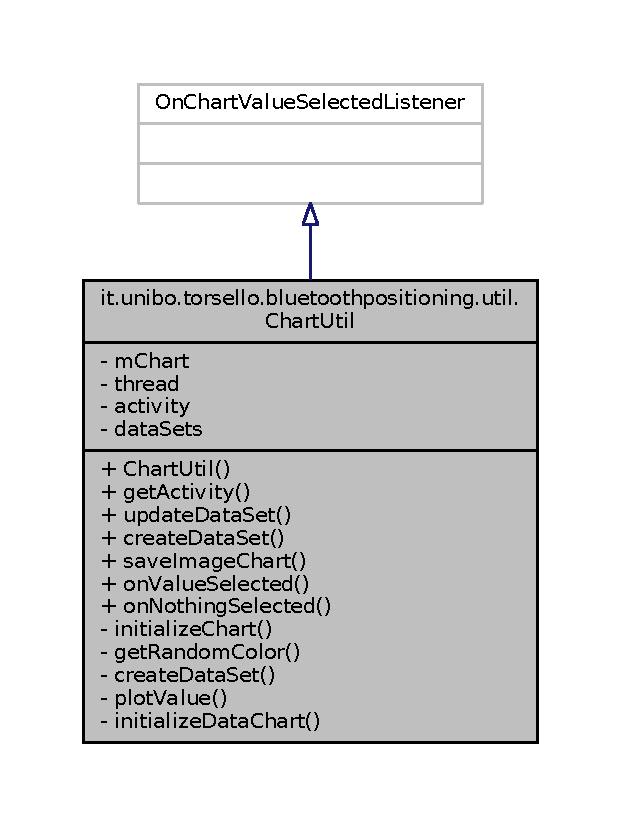
\includegraphics[width=298pt]{classit_1_1unibo_1_1torsello_1_1bluetoothpositioning_1_1util_1_1ChartUtil__inherit__graph}
\end{center}
\end{figure}


Diagramma di collaborazione per it.\+unibo.\+torsello.\+bluetoothpositioning.\+util.\+Chart\+Util\+:
\nopagebreak
\begin{figure}[H]
\begin{center}
\leavevmode
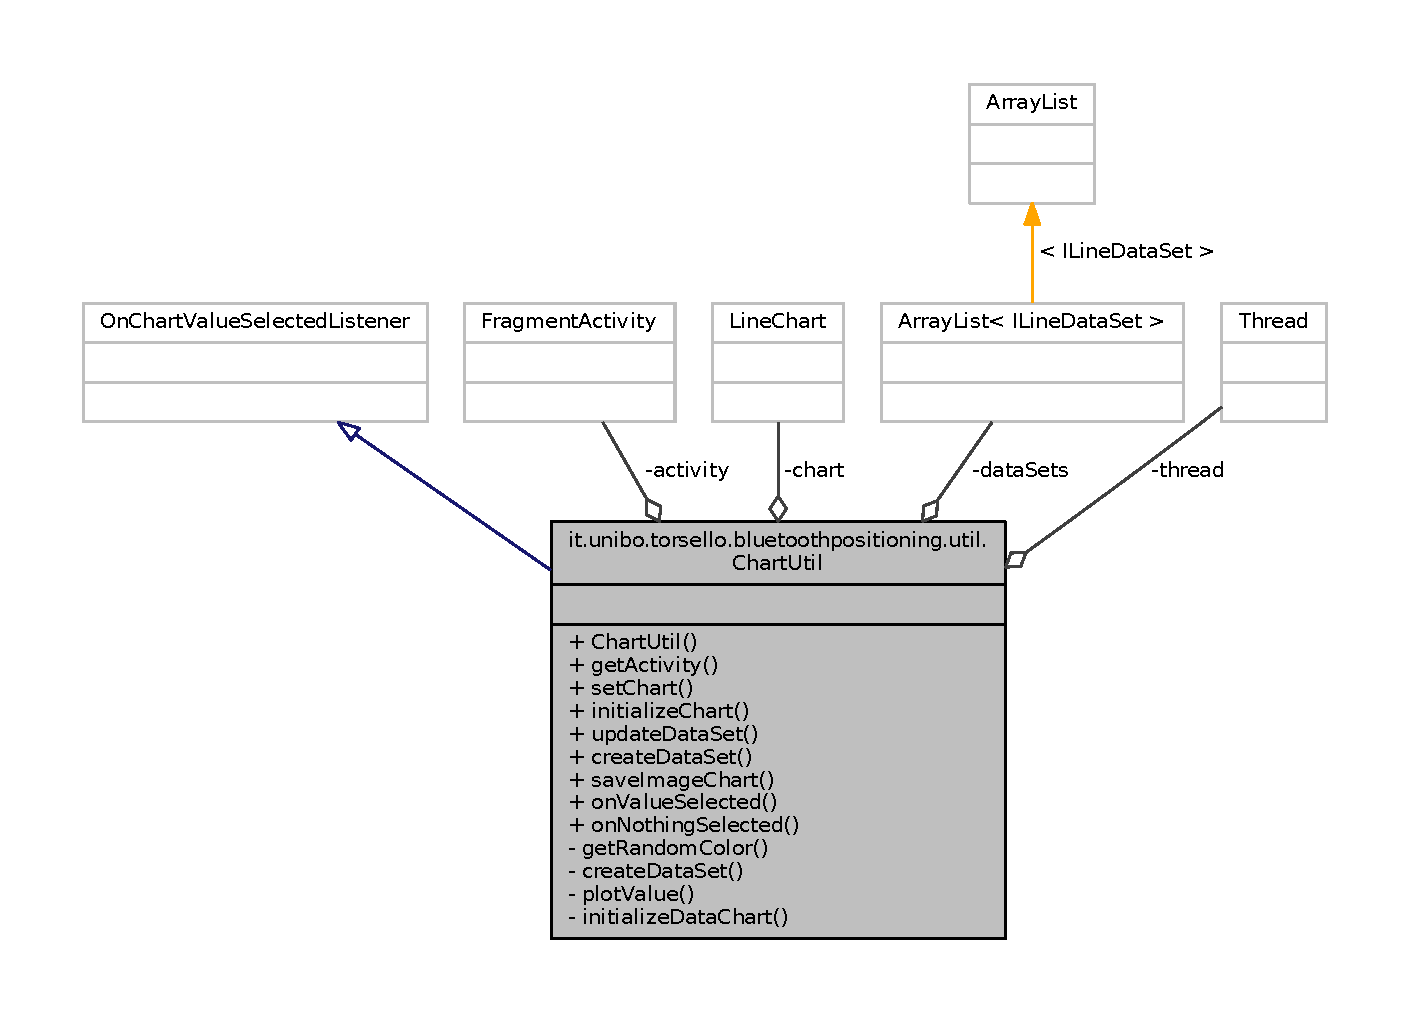
\includegraphics[width=350pt]{classit_1_1unibo_1_1torsello_1_1bluetoothpositioning_1_1util_1_1ChartUtil__coll__graph}
\end{center}
\end{figure}
\subsubsection*{Membri pubblici}
\begin{DoxyCompactItemize}
\item 
\hyperlink{classit_1_1unibo_1_1torsello_1_1bluetoothpositioning_1_1util_1_1ChartUtil_a255b439c7574dc7858355e3fc71ca6f7_a255b439c7574dc7858355e3fc71ca6f7}{Chart\+Util} (Fragment\+Activity fragment\+Activity)
\item 
Fragment\+Activity \hyperlink{classit_1_1unibo_1_1torsello_1_1bluetoothpositioning_1_1util_1_1ChartUtil_a59150a6d20b6d0ad2fcf8c1ba858d355_a59150a6d20b6d0ad2fcf8c1ba858d355}{get\+Activity} ()
\item 
void \hyperlink{classit_1_1unibo_1_1torsello_1_1bluetoothpositioning_1_1util_1_1ChartUtil_a26e84414723ff1ca38d8f2907ed3322e_a26e84414723ff1ca38d8f2907ed3322e}{set\+Chart} (Line\+Chart \hyperlink{classit_1_1unibo_1_1torsello_1_1bluetoothpositioning_1_1util_1_1ChartUtil_a6c34176fdfb85bac1d3aa1529b49ad5f_a6c34176fdfb85bac1d3aa1529b49ad5f}{chart})
\item 
void \hyperlink{classit_1_1unibo_1_1torsello_1_1bluetoothpositioning_1_1util_1_1ChartUtil_aab1a6bd41cbf8228c53d633af6b89bb7_aab1a6bd41cbf8228c53d633af6b89bb7}{initialize\+Chart} ()
\item 
void \hyperlink{classit_1_1unibo_1_1torsello_1_1bluetoothpositioning_1_1util_1_1ChartUtil_aa9bda04d2c2058fb1b3fcd72c5a7471d_aa9bda04d2c2058fb1b3fcd72c5a7471d}{update\+Data\+Set} (final Array\+List$<$ Double $>$ double\+Array\+List)
\item 
void \hyperlink{classit_1_1unibo_1_1torsello_1_1bluetoothpositioning_1_1util_1_1ChartUtil_a7460cb57f8ad402dc522b592bc40f7b2_a7460cb57f8ad402dc522b592bc40f7b2}{create\+Data\+Set} (Array\+List$<$ String $>$ args)
\item 
void \hyperlink{classit_1_1unibo_1_1torsello_1_1bluetoothpositioning_1_1util_1_1ChartUtil_afdbdcf15b073da5b03613dbccc7681a9_afdbdcf15b073da5b03613dbccc7681a9}{save\+Image\+Chart} (String chart\+Name, String formatted\+Date)
\item 
void \hyperlink{classit_1_1unibo_1_1torsello_1_1bluetoothpositioning_1_1util_1_1ChartUtil_a7f7609b8236d269e4f272f717b0b0294_a7f7609b8236d269e4f272f717b0b0294}{on\+Value\+Selected} (Entry e, Highlight h)
\item 
void \hyperlink{classit_1_1unibo_1_1torsello_1_1bluetoothpositioning_1_1util_1_1ChartUtil_a7e7f15aebf87926e19bc9e1ece289fde_a7e7f15aebf87926e19bc9e1ece289fde}{on\+Nothing\+Selected} ()
\end{DoxyCompactItemize}
\subsubsection*{Membri privati}
\begin{DoxyCompactItemize}
\item 
int \hyperlink{classit_1_1unibo_1_1torsello_1_1bluetoothpositioning_1_1util_1_1ChartUtil_ac7dc0a849201a4a3c932fd525435b397_ac7dc0a849201a4a3c932fd525435b397}{get\+Random\+Color} ()
\item 
Line\+Data\+Set \hyperlink{classit_1_1unibo_1_1torsello_1_1bluetoothpositioning_1_1util_1_1ChartUtil_a7e24ac167fd4955090e04024b11c6c31_a7e24ac167fd4955090e04024b11c6c31}{create\+Data\+Set} (String name\+Data\+Set, int color)
\item 
void \hyperlink{classit_1_1unibo_1_1torsello_1_1bluetoothpositioning_1_1util_1_1ChartUtil_a86398d4aca978fbfc10c71039191635e_a86398d4aca978fbfc10c71039191635e}{plot\+Value} (Line\+Data data, int index, Double value)
\item 
void \hyperlink{classit_1_1unibo_1_1torsello_1_1bluetoothpositioning_1_1util_1_1ChartUtil_a3393d9aa353849188c02a63d64f2dd2d_a3393d9aa353849188c02a63d64f2dd2d}{initialize\+Data\+Chart} (Array\+List$<$ I\+Line\+Data\+Set $>$ \hyperlink{classit_1_1unibo_1_1torsello_1_1bluetoothpositioning_1_1util_1_1ChartUtil_aa98bcaa2d5ba444b91cdc029768d380a_aa98bcaa2d5ba444b91cdc029768d380a}{data\+Sets})
\end{DoxyCompactItemize}
\subsubsection*{Attributi privati}
\begin{DoxyCompactItemize}
\item 
Line\+Chart \hyperlink{classit_1_1unibo_1_1torsello_1_1bluetoothpositioning_1_1util_1_1ChartUtil_a6c34176fdfb85bac1d3aa1529b49ad5f_a6c34176fdfb85bac1d3aa1529b49ad5f}{chart}
\item 
Thread \hyperlink{classit_1_1unibo_1_1torsello_1_1bluetoothpositioning_1_1util_1_1ChartUtil_ac73af861c9ca49e226fe1218cef6c572_ac73af861c9ca49e226fe1218cef6c572}{thread}
\item 
Fragment\+Activity \hyperlink{classit_1_1unibo_1_1torsello_1_1bluetoothpositioning_1_1util_1_1ChartUtil_acf9c1988f7aaacc3f3354ac7e9eeef6a_acf9c1988f7aaacc3f3354ac7e9eeef6a}{activity}
\item 
Array\+List$<$ I\+Line\+Data\+Set $>$ \hyperlink{classit_1_1unibo_1_1torsello_1_1bluetoothpositioning_1_1util_1_1ChartUtil_aa98bcaa2d5ba444b91cdc029768d380a_aa98bcaa2d5ba444b91cdc029768d380a}{data\+Sets}
\end{DoxyCompactItemize}


\subsubsection{Descrizione dettagliata}
Created by Federico Torsello. \href{mailto:federico.torsello@studio.unibo.it}{\tt federico.\+torsello@studio.\+unibo.\+it} 

\subsubsection{Documentazione dei costruttori e dei distruttori}
\hypertarget{classit_1_1unibo_1_1torsello_1_1bluetoothpositioning_1_1util_1_1ChartUtil_a255b439c7574dc7858355e3fc71ca6f7_a255b439c7574dc7858355e3fc71ca6f7}{}\label{classit_1_1unibo_1_1torsello_1_1bluetoothpositioning_1_1util_1_1ChartUtil_a255b439c7574dc7858355e3fc71ca6f7_a255b439c7574dc7858355e3fc71ca6f7} 
\index{it\+::unibo\+::torsello\+::bluetoothpositioning\+::util\+::\+Chart\+Util@{it\+::unibo\+::torsello\+::bluetoothpositioning\+::util\+::\+Chart\+Util}!Chart\+Util@{Chart\+Util}}
\index{Chart\+Util@{Chart\+Util}!it\+::unibo\+::torsello\+::bluetoothpositioning\+::util\+::\+Chart\+Util@{it\+::unibo\+::torsello\+::bluetoothpositioning\+::util\+::\+Chart\+Util}}
\paragraph{\texorpdfstring{Chart\+Util()}{ChartUtil()}}
{\footnotesize\ttfamily it.\+unibo.\+torsello.\+bluetoothpositioning.\+util.\+Chart\+Util.\+Chart\+Util (\begin{DoxyParamCaption}\item[{Fragment\+Activity}]{fragment\+Activity }\end{DoxyParamCaption})}


\begin{DoxyCode}
42                                                         \{
43         this.\hyperlink{classit_1_1unibo_1_1torsello_1_1bluetoothpositioning_1_1util_1_1ChartUtil_acf9c1988f7aaacc3f3354ac7e9eeef6a_acf9c1988f7aaacc3f3354ac7e9eeef6a}{activity} = fragmentActivity;
44     \}
\end{DoxyCode}


\subsubsection{Documentazione delle funzioni membro}
\hypertarget{classit_1_1unibo_1_1torsello_1_1bluetoothpositioning_1_1util_1_1ChartUtil_a7460cb57f8ad402dc522b592bc40f7b2_a7460cb57f8ad402dc522b592bc40f7b2}{}\label{classit_1_1unibo_1_1torsello_1_1bluetoothpositioning_1_1util_1_1ChartUtil_a7460cb57f8ad402dc522b592bc40f7b2_a7460cb57f8ad402dc522b592bc40f7b2} 
\index{it\+::unibo\+::torsello\+::bluetoothpositioning\+::util\+::\+Chart\+Util@{it\+::unibo\+::torsello\+::bluetoothpositioning\+::util\+::\+Chart\+Util}!create\+Data\+Set@{create\+Data\+Set}}
\index{create\+Data\+Set@{create\+Data\+Set}!it\+::unibo\+::torsello\+::bluetoothpositioning\+::util\+::\+Chart\+Util@{it\+::unibo\+::torsello\+::bluetoothpositioning\+::util\+::\+Chart\+Util}}
\paragraph{\texorpdfstring{create\+Data\+Set()}{createDataSet()}\hspace{0.1cm}{\footnotesize\ttfamily [1/2]}}
{\footnotesize\ttfamily void it.\+unibo.\+torsello.\+bluetoothpositioning.\+util.\+Chart\+Util.\+create\+Data\+Set (\begin{DoxyParamCaption}\item[{Array\+List$<$ String $>$}]{args }\end{DoxyParamCaption})}


\begin{DoxyCode}
133                                                       \{
134         \textcolor{comment}{// create a dataset and give it a type}
135 
136         \textcolor{keywordflow}{for} (String s : args) \{
137             \textcolor{keywordflow}{if} (s != null) \{
138                 \textcolor{keywordflow}{if} (s.equals(\hyperlink{classit_1_1unibo_1_1torsello_1_1bluetoothpositioning_1_1util_1_1ChartUtil_a59150a6d20b6d0ad2fcf8c1ba858d355_a59150a6d20b6d0ad2fcf8c1ba858d355}{getActivity}().getString(R.string.chart\_arduino))) \{
139                     \hyperlink{classit_1_1unibo_1_1torsello_1_1bluetoothpositioning_1_1util_1_1ChartUtil_aa98bcaa2d5ba444b91cdc029768d380a_aa98bcaa2d5ba444b91cdc029768d380a}{dataSets}.add(\hyperlink{classit_1_1unibo_1_1torsello_1_1bluetoothpositioning_1_1util_1_1ChartUtil_a7460cb57f8ad402dc522b592bc40f7b2_a7460cb57f8ad402dc522b592bc40f7b2}{createDataSet}(s, Color.RED));
140                 \} \textcolor{keywordflow}{else} \{
141                     \hyperlink{classit_1_1unibo_1_1torsello_1_1bluetoothpositioning_1_1util_1_1ChartUtil_aa98bcaa2d5ba444b91cdc029768d380a_aa98bcaa2d5ba444b91cdc029768d380a}{dataSets}.add(\hyperlink{classit_1_1unibo_1_1torsello_1_1bluetoothpositioning_1_1util_1_1ChartUtil_a7460cb57f8ad402dc522b592bc40f7b2_a7460cb57f8ad402dc522b592bc40f7b2}{createDataSet}(s, 
      \hyperlink{classit_1_1unibo_1_1torsello_1_1bluetoothpositioning_1_1util_1_1ChartUtil_ac7dc0a849201a4a3c932fd525435b397_ac7dc0a849201a4a3c932fd525435b397}{getRandomColor}()));
142                 \}
143             \}
144         \}
145 
146     \}
\end{DoxyCode}
\hypertarget{classit_1_1unibo_1_1torsello_1_1bluetoothpositioning_1_1util_1_1ChartUtil_a7e24ac167fd4955090e04024b11c6c31_a7e24ac167fd4955090e04024b11c6c31}{}\label{classit_1_1unibo_1_1torsello_1_1bluetoothpositioning_1_1util_1_1ChartUtil_a7e24ac167fd4955090e04024b11c6c31_a7e24ac167fd4955090e04024b11c6c31} 
\index{it\+::unibo\+::torsello\+::bluetoothpositioning\+::util\+::\+Chart\+Util@{it\+::unibo\+::torsello\+::bluetoothpositioning\+::util\+::\+Chart\+Util}!create\+Data\+Set@{create\+Data\+Set}}
\index{create\+Data\+Set@{create\+Data\+Set}!it\+::unibo\+::torsello\+::bluetoothpositioning\+::util\+::\+Chart\+Util@{it\+::unibo\+::torsello\+::bluetoothpositioning\+::util\+::\+Chart\+Util}}
\paragraph{\texorpdfstring{create\+Data\+Set()}{createDataSet()}\hspace{0.1cm}{\footnotesize\ttfamily [2/2]}}
{\footnotesize\ttfamily Line\+Data\+Set it.\+unibo.\+torsello.\+bluetoothpositioning.\+util.\+Chart\+Util.\+create\+Data\+Set (\begin{DoxyParamCaption}\item[{String}]{name\+Data\+Set,  }\item[{int}]{color }\end{DoxyParamCaption})\hspace{0.3cm}{\ttfamily [private]}}


\begin{DoxyCode}
157                                                                      \{
158         LineDataSet \textcolor{keyword}{set} = \textcolor{keyword}{new} LineDataSet(null, nameDataSet);
159         \textcolor{keyword}{set}.setColor(color);
160         \textcolor{keywordflow}{return} \textcolor{keyword}{set};
161     \}
\end{DoxyCode}
\hypertarget{classit_1_1unibo_1_1torsello_1_1bluetoothpositioning_1_1util_1_1ChartUtil_a59150a6d20b6d0ad2fcf8c1ba858d355_a59150a6d20b6d0ad2fcf8c1ba858d355}{}\label{classit_1_1unibo_1_1torsello_1_1bluetoothpositioning_1_1util_1_1ChartUtil_a59150a6d20b6d0ad2fcf8c1ba858d355_a59150a6d20b6d0ad2fcf8c1ba858d355} 
\index{it\+::unibo\+::torsello\+::bluetoothpositioning\+::util\+::\+Chart\+Util@{it\+::unibo\+::torsello\+::bluetoothpositioning\+::util\+::\+Chart\+Util}!get\+Activity@{get\+Activity}}
\index{get\+Activity@{get\+Activity}!it\+::unibo\+::torsello\+::bluetoothpositioning\+::util\+::\+Chart\+Util@{it\+::unibo\+::torsello\+::bluetoothpositioning\+::util\+::\+Chart\+Util}}
\paragraph{\texorpdfstring{get\+Activity()}{getActivity()}}
{\footnotesize\ttfamily Fragment\+Activity it.\+unibo.\+torsello.\+bluetoothpositioning.\+util.\+Chart\+Util.\+get\+Activity (\begin{DoxyParamCaption}{ }\end{DoxyParamCaption})}


\begin{DoxyCode}
46                                           \{
47         \textcolor{keywordflow}{return} \hyperlink{classit_1_1unibo_1_1torsello_1_1bluetoothpositioning_1_1util_1_1ChartUtil_acf9c1988f7aaacc3f3354ac7e9eeef6a_acf9c1988f7aaacc3f3354ac7e9eeef6a}{activity};
48     \}
\end{DoxyCode}
\hypertarget{classit_1_1unibo_1_1torsello_1_1bluetoothpositioning_1_1util_1_1ChartUtil_ac7dc0a849201a4a3c932fd525435b397_ac7dc0a849201a4a3c932fd525435b397}{}\label{classit_1_1unibo_1_1torsello_1_1bluetoothpositioning_1_1util_1_1ChartUtil_ac7dc0a849201a4a3c932fd525435b397_ac7dc0a849201a4a3c932fd525435b397} 
\index{it\+::unibo\+::torsello\+::bluetoothpositioning\+::util\+::\+Chart\+Util@{it\+::unibo\+::torsello\+::bluetoothpositioning\+::util\+::\+Chart\+Util}!get\+Random\+Color@{get\+Random\+Color}}
\index{get\+Random\+Color@{get\+Random\+Color}!it\+::unibo\+::torsello\+::bluetoothpositioning\+::util\+::\+Chart\+Util@{it\+::unibo\+::torsello\+::bluetoothpositioning\+::util\+::\+Chart\+Util}}
\paragraph{\texorpdfstring{get\+Random\+Color()}{getRandomColor()}}
{\footnotesize\ttfamily int it.\+unibo.\+torsello.\+bluetoothpositioning.\+util.\+Chart\+Util.\+get\+Random\+Color (\begin{DoxyParamCaption}{ }\end{DoxyParamCaption})\hspace{0.3cm}{\ttfamily [private]}}


\begin{DoxyCode}
148                                  \{
149         Random rnd = \textcolor{keyword}{new} Random();
150         \textcolor{keywordtype}{int} color = 0;
151         \textcolor{keywordflow}{while} (color == 0) \{
152             color = Color.argb(255, rnd.nextInt(255), rnd.nextInt(255), rnd.nextInt(255));
153         \}
154         \textcolor{keywordflow}{return} color;
155     \}
\end{DoxyCode}
\hypertarget{classit_1_1unibo_1_1torsello_1_1bluetoothpositioning_1_1util_1_1ChartUtil_aab1a6bd41cbf8228c53d633af6b89bb7_aab1a6bd41cbf8228c53d633af6b89bb7}{}\label{classit_1_1unibo_1_1torsello_1_1bluetoothpositioning_1_1util_1_1ChartUtil_aab1a6bd41cbf8228c53d633af6b89bb7_aab1a6bd41cbf8228c53d633af6b89bb7} 
\index{it\+::unibo\+::torsello\+::bluetoothpositioning\+::util\+::\+Chart\+Util@{it\+::unibo\+::torsello\+::bluetoothpositioning\+::util\+::\+Chart\+Util}!initialize\+Chart@{initialize\+Chart}}
\index{initialize\+Chart@{initialize\+Chart}!it\+::unibo\+::torsello\+::bluetoothpositioning\+::util\+::\+Chart\+Util@{it\+::unibo\+::torsello\+::bluetoothpositioning\+::util\+::\+Chart\+Util}}
\paragraph{\texorpdfstring{initialize\+Chart()}{initializeChart()}}
{\footnotesize\ttfamily void it.\+unibo.\+torsello.\+bluetoothpositioning.\+util.\+Chart\+Util.\+initialize\+Chart (\begin{DoxyParamCaption}{ }\end{DoxyParamCaption})}


\begin{DoxyCode}
54                                   \{
55         \hyperlink{classit_1_1unibo_1_1torsello_1_1bluetoothpositioning_1_1util_1_1ChartUtil_aa98bcaa2d5ba444b91cdc029768d380a_aa98bcaa2d5ba444b91cdc029768d380a}{dataSets} = \textcolor{keyword}{new} ArrayList<ILineDataSet>();
56 
57         \hyperlink{classit_1_1unibo_1_1torsello_1_1bluetoothpositioning_1_1util_1_1ChartUtil_a6c34176fdfb85bac1d3aa1529b49ad5f_a6c34176fdfb85bac1d3aa1529b49ad5f}{chart}.setOnChartValueSelectedListener(\textcolor{keyword}{this});
58 
59         \textcolor{comment}{// no description text}
60         \hyperlink{classit_1_1unibo_1_1torsello_1_1bluetoothpositioning_1_1util_1_1ChartUtil_a6c34176fdfb85bac1d3aa1529b49ad5f_a6c34176fdfb85bac1d3aa1529b49ad5f}{chart}.setDescription(\textcolor{stringliteral}{""});
61         \hyperlink{classit_1_1unibo_1_1torsello_1_1bluetoothpositioning_1_1util_1_1ChartUtil_a6c34176fdfb85bac1d3aa1529b49ad5f_a6c34176fdfb85bac1d3aa1529b49ad5f}{chart}.setNoDataTextDescription(\textcolor{stringliteral}{"You need to provide data for the chart."});
62 
63         \hyperlink{classit_1_1unibo_1_1torsello_1_1bluetoothpositioning_1_1util_1_1ChartUtil_a6c34176fdfb85bac1d3aa1529b49ad5f_a6c34176fdfb85bac1d3aa1529b49ad5f}{chart}.setDrawGridBackground(\textcolor{keyword}{true});
64 
65         \textcolor{comment}{// if disabled, scaling can be done on x- and y-axis separately}
66         \hyperlink{classit_1_1unibo_1_1torsello_1_1bluetoothpositioning_1_1util_1_1ChartUtil_a6c34176fdfb85bac1d3aa1529b49ad5f_a6c34176fdfb85bac1d3aa1529b49ad5f}{chart}.setPinchZoom(\textcolor{keyword}{true});
67 
68         \textcolor{comment}{// set an alternative background color}
69         \hyperlink{classit_1_1unibo_1_1torsello_1_1bluetoothpositioning_1_1util_1_1ChartUtil_a6c34176fdfb85bac1d3aa1529b49ad5f_a6c34176fdfb85bac1d3aa1529b49ad5f}{chart}.setBackgroundColor(Color.LTGRAY);
70 
71         Typeface mTfLight = Typeface.createFromAsset(\hyperlink{classit_1_1unibo_1_1torsello_1_1bluetoothpositioning_1_1util_1_1ChartUtil_a59150a6d20b6d0ad2fcf8c1ba858d355_a59150a6d20b6d0ad2fcf8c1ba858d355}{getActivity}().getAssets(), \textcolor{stringliteral}{"
      OpenSans-Light.ttf"});
72         Typeface mTfBold = Typeface.createFromAsset(\hyperlink{classit_1_1unibo_1_1torsello_1_1bluetoothpositioning_1_1util_1_1ChartUtil_a59150a6d20b6d0ad2fcf8c1ba858d355_a59150a6d20b6d0ad2fcf8c1ba858d355}{getActivity}().getAssets(), \textcolor{stringliteral}{"
      OpenSans-Bold.ttf"});
73 
74         \textcolor{comment}{// get the legend (only possible after setting data)}
75         Legend l = \hyperlink{classit_1_1unibo_1_1torsello_1_1bluetoothpositioning_1_1util_1_1ChartUtil_a6c34176fdfb85bac1d3aa1529b49ad5f_a6c34176fdfb85bac1d3aa1529b49ad5f}{chart}.getLegend();
76 \textcolor{comment}{//        l.setPosition(Legend.LegendPosition.RIGHT\_OF\_CHART);}
77 \textcolor{comment}{//        l.setOrientation(Legend.LegendOrientation.VERTICAL);}
78         l.setXEntrySpace(7f);
79         l.setYEntrySpace(7f);
80 
81         XAxis xl = \hyperlink{classit_1_1unibo_1_1torsello_1_1bluetoothpositioning_1_1util_1_1ChartUtil_a6c34176fdfb85bac1d3aa1529b49ad5f_a6c34176fdfb85bac1d3aa1529b49ad5f}{chart}.getXAxis();
82         xl.setTypeface(mTfLight);
83         xl.setGridColor(Color.LTGRAY);
84         xl.setTextColor(Color.WHITE);
85 
86         YAxis leftAxis = \hyperlink{classit_1_1unibo_1_1torsello_1_1bluetoothpositioning_1_1util_1_1ChartUtil_a6c34176fdfb85bac1d3aa1529b49ad5f_a6c34176fdfb85bac1d3aa1529b49ad5f}{chart}.getAxisLeft();
87         leftAxis.setTypeface(mTfLight);
88         leftAxis.setTextColor(Color.WHITE);
89 
90         YAxis rightAxis = \hyperlink{classit_1_1unibo_1_1torsello_1_1bluetoothpositioning_1_1util_1_1ChartUtil_a6c34176fdfb85bac1d3aa1529b49ad5f_a6c34176fdfb85bac1d3aa1529b49ad5f}{chart}.getAxisRight();
91         rightAxis.setTypeface(mTfBold);
92 
93     \}
\end{DoxyCode}
\hypertarget{classit_1_1unibo_1_1torsello_1_1bluetoothpositioning_1_1util_1_1ChartUtil_a3393d9aa353849188c02a63d64f2dd2d_a3393d9aa353849188c02a63d64f2dd2d}{}\label{classit_1_1unibo_1_1torsello_1_1bluetoothpositioning_1_1util_1_1ChartUtil_a3393d9aa353849188c02a63d64f2dd2d_a3393d9aa353849188c02a63d64f2dd2d} 
\index{it\+::unibo\+::torsello\+::bluetoothpositioning\+::util\+::\+Chart\+Util@{it\+::unibo\+::torsello\+::bluetoothpositioning\+::util\+::\+Chart\+Util}!initialize\+Data\+Chart@{initialize\+Data\+Chart}}
\index{initialize\+Data\+Chart@{initialize\+Data\+Chart}!it\+::unibo\+::torsello\+::bluetoothpositioning\+::util\+::\+Chart\+Util@{it\+::unibo\+::torsello\+::bluetoothpositioning\+::util\+::\+Chart\+Util}}
\paragraph{\texorpdfstring{initialize\+Data\+Chart()}{initializeDataChart()}}
{\footnotesize\ttfamily void it.\+unibo.\+torsello.\+bluetoothpositioning.\+util.\+Chart\+Util.\+initialize\+Data\+Chart (\begin{DoxyParamCaption}\item[{Array\+List$<$ I\+Line\+Data\+Set $>$}]{data\+Sets }\end{DoxyParamCaption})\hspace{0.3cm}{\ttfamily [private]}}


\begin{DoxyCode}
181                                                                        \{
182 
183         \textcolor{comment}{// create a data object with the datasets}
184         LineData lineData = \textcolor{keyword}{new} LineData(\hyperlink{classit_1_1unibo_1_1torsello_1_1bluetoothpositioning_1_1util_1_1ChartUtil_aa98bcaa2d5ba444b91cdc029768d380a_aa98bcaa2d5ba444b91cdc029768d380a}{dataSets});
185         lineData.setValueTextColor(Color.RED);
186         lineData.setValueTextSize(9f);
187         lineData.setValueFormatter(\textcolor{keyword}{new} DefaultValueFormatter(2));
188 
189         \textcolor{comment}{// set data}
190         \hyperlink{classit_1_1unibo_1_1torsello_1_1bluetoothpositioning_1_1util_1_1ChartUtil_a6c34176fdfb85bac1d3aa1529b49ad5f_a6c34176fdfb85bac1d3aa1529b49ad5f}{chart}.setData(lineData);
191     \}
\end{DoxyCode}
\hypertarget{classit_1_1unibo_1_1torsello_1_1bluetoothpositioning_1_1util_1_1ChartUtil_a7e7f15aebf87926e19bc9e1ece289fde_a7e7f15aebf87926e19bc9e1ece289fde}{}\label{classit_1_1unibo_1_1torsello_1_1bluetoothpositioning_1_1util_1_1ChartUtil_a7e7f15aebf87926e19bc9e1ece289fde_a7e7f15aebf87926e19bc9e1ece289fde} 
\index{it\+::unibo\+::torsello\+::bluetoothpositioning\+::util\+::\+Chart\+Util@{it\+::unibo\+::torsello\+::bluetoothpositioning\+::util\+::\+Chart\+Util}!on\+Nothing\+Selected@{on\+Nothing\+Selected}}
\index{on\+Nothing\+Selected@{on\+Nothing\+Selected}!it\+::unibo\+::torsello\+::bluetoothpositioning\+::util\+::\+Chart\+Util@{it\+::unibo\+::torsello\+::bluetoothpositioning\+::util\+::\+Chart\+Util}}
\paragraph{\texorpdfstring{on\+Nothing\+Selected()}{onNothingSelected()}}
{\footnotesize\ttfamily void it.\+unibo.\+torsello.\+bluetoothpositioning.\+util.\+Chart\+Util.\+on\+Nothing\+Selected (\begin{DoxyParamCaption}{ }\end{DoxyParamCaption})}


\begin{DoxyCode}
209                                     \{
210 \textcolor{comment}{//        Log.i("Nothing selected", "Nothing selected.");}
211     \}
\end{DoxyCode}
\hypertarget{classit_1_1unibo_1_1torsello_1_1bluetoothpositioning_1_1util_1_1ChartUtil_a7f7609b8236d269e4f272f717b0b0294_a7f7609b8236d269e4f272f717b0b0294}{}\label{classit_1_1unibo_1_1torsello_1_1bluetoothpositioning_1_1util_1_1ChartUtil_a7f7609b8236d269e4f272f717b0b0294_a7f7609b8236d269e4f272f717b0b0294} 
\index{it\+::unibo\+::torsello\+::bluetoothpositioning\+::util\+::\+Chart\+Util@{it\+::unibo\+::torsello\+::bluetoothpositioning\+::util\+::\+Chart\+Util}!on\+Value\+Selected@{on\+Value\+Selected}}
\index{on\+Value\+Selected@{on\+Value\+Selected}!it\+::unibo\+::torsello\+::bluetoothpositioning\+::util\+::\+Chart\+Util@{it\+::unibo\+::torsello\+::bluetoothpositioning\+::util\+::\+Chart\+Util}}
\paragraph{\texorpdfstring{on\+Value\+Selected()}{onValueSelected()}}
{\footnotesize\ttfamily void it.\+unibo.\+torsello.\+bluetoothpositioning.\+util.\+Chart\+Util.\+on\+Value\+Selected (\begin{DoxyParamCaption}\item[{Entry}]{e,  }\item[{Highlight}]{h }\end{DoxyParamCaption})}


\begin{DoxyCode}
203                                                       \{
204         Snackbar.make(\hyperlink{classit_1_1unibo_1_1torsello_1_1bluetoothpositioning_1_1util_1_1ChartUtil_a59150a6d20b6d0ad2fcf8c1ba858d355_a59150a6d20b6d0ad2fcf8c1ba858d355}{getActivity}().findViewById(R.id.fab), e.copy() + \textcolor{stringliteral}{" selected"}
205                 , Snackbar.LENGTH\_SHORT).show();
206     \}
\end{DoxyCode}
\hypertarget{classit_1_1unibo_1_1torsello_1_1bluetoothpositioning_1_1util_1_1ChartUtil_a86398d4aca978fbfc10c71039191635e_a86398d4aca978fbfc10c71039191635e}{}\label{classit_1_1unibo_1_1torsello_1_1bluetoothpositioning_1_1util_1_1ChartUtil_a86398d4aca978fbfc10c71039191635e_a86398d4aca978fbfc10c71039191635e} 
\index{it\+::unibo\+::torsello\+::bluetoothpositioning\+::util\+::\+Chart\+Util@{it\+::unibo\+::torsello\+::bluetoothpositioning\+::util\+::\+Chart\+Util}!plot\+Value@{plot\+Value}}
\index{plot\+Value@{plot\+Value}!it\+::unibo\+::torsello\+::bluetoothpositioning\+::util\+::\+Chart\+Util@{it\+::unibo\+::torsello\+::bluetoothpositioning\+::util\+::\+Chart\+Util}}
\paragraph{\texorpdfstring{plot\+Value()}{plotValue()}}
{\footnotesize\ttfamily void it.\+unibo.\+torsello.\+bluetoothpositioning.\+util.\+Chart\+Util.\+plot\+Value (\begin{DoxyParamCaption}\item[{Line\+Data}]{data,  }\item[{int}]{index,  }\item[{Double}]{value }\end{DoxyParamCaption})\hspace{0.3cm}{\ttfamily [private]}}


\begin{DoxyCode}
163                                                                    \{
164 
165         ILineDataSet \textcolor{keyword}{set} = data.getDataSetByIndex(index);
166 
167         \textcolor{keyword}{set}.addEntry(\textcolor{keyword}{new} Entry(\textcolor{keyword}{set}.getEntryCount(), value.floatValue()));
168 
169         data.notifyDataChanged();
170 
171         \textcolor{comment}{// let the chart know it's data has changed}
172         \hyperlink{classit_1_1unibo_1_1torsello_1_1bluetoothpositioning_1_1util_1_1ChartUtil_a6c34176fdfb85bac1d3aa1529b49ad5f_a6c34176fdfb85bac1d3aa1529b49ad5f}{chart}.notifyDataSetChanged();
173 
174         \textcolor{comment}{// limit the number of visible entries}
175         \hyperlink{classit_1_1unibo_1_1torsello_1_1bluetoothpositioning_1_1util_1_1ChartUtil_a6c34176fdfb85bac1d3aa1529b49ad5f_a6c34176fdfb85bac1d3aa1529b49ad5f}{chart}.setVisibleXRangeMaximum(10);
176 
177         \textcolor{comment}{// move to the latest entry}
178         \hyperlink{classit_1_1unibo_1_1torsello_1_1bluetoothpositioning_1_1util_1_1ChartUtil_a6c34176fdfb85bac1d3aa1529b49ad5f_a6c34176fdfb85bac1d3aa1529b49ad5f}{chart}.moveViewToX(data.getEntryCount());
179     \}
\end{DoxyCode}
\hypertarget{classit_1_1unibo_1_1torsello_1_1bluetoothpositioning_1_1util_1_1ChartUtil_afdbdcf15b073da5b03613dbccc7681a9_afdbdcf15b073da5b03613dbccc7681a9}{}\label{classit_1_1unibo_1_1torsello_1_1bluetoothpositioning_1_1util_1_1ChartUtil_afdbdcf15b073da5b03613dbccc7681a9_afdbdcf15b073da5b03613dbccc7681a9} 
\index{it\+::unibo\+::torsello\+::bluetoothpositioning\+::util\+::\+Chart\+Util@{it\+::unibo\+::torsello\+::bluetoothpositioning\+::util\+::\+Chart\+Util}!save\+Image\+Chart@{save\+Image\+Chart}}
\index{save\+Image\+Chart@{save\+Image\+Chart}!it\+::unibo\+::torsello\+::bluetoothpositioning\+::util\+::\+Chart\+Util@{it\+::unibo\+::torsello\+::bluetoothpositioning\+::util\+::\+Chart\+Util}}
\paragraph{\texorpdfstring{save\+Image\+Chart()}{saveImageChart()}}
{\footnotesize\ttfamily void it.\+unibo.\+torsello.\+bluetoothpositioning.\+util.\+Chart\+Util.\+save\+Image\+Chart (\begin{DoxyParamCaption}\item[{String}]{chart\+Name,  }\item[{String}]{formatted\+Date }\end{DoxyParamCaption})}


\begin{DoxyCode}
193                                                                        \{
194         String nameImage = chartName + \textcolor{stringliteral}{" "} + System.currentTimeMillis();
195         \hyperlink{classit_1_1unibo_1_1torsello_1_1bluetoothpositioning_1_1util_1_1ChartUtil_a6c34176fdfb85bac1d3aa1529b49ad5f_a6c34176fdfb85bac1d3aa1529b49ad5f}{chart}.saveToGallery(nameImage, chartName
196                 + \textcolor{stringliteral}{" - "} + formattedDate, null, Bitmap.CompressFormat.JPEG, 100);
197 
198         Snackbar.make(\hyperlink{classit_1_1unibo_1_1torsello_1_1bluetoothpositioning_1_1util_1_1ChartUtil_a59150a6d20b6d0ad2fcf8c1ba858d355_a59150a6d20b6d0ad2fcf8c1ba858d355}{getActivity}().findViewById(R.id.fab), chartName + \textcolor{stringliteral}{" stored"}
199                 , Snackbar.LENGTH\_SHORT).show();
200     \}
\end{DoxyCode}
\hypertarget{classit_1_1unibo_1_1torsello_1_1bluetoothpositioning_1_1util_1_1ChartUtil_a26e84414723ff1ca38d8f2907ed3322e_a26e84414723ff1ca38d8f2907ed3322e}{}\label{classit_1_1unibo_1_1torsello_1_1bluetoothpositioning_1_1util_1_1ChartUtil_a26e84414723ff1ca38d8f2907ed3322e_a26e84414723ff1ca38d8f2907ed3322e} 
\index{it\+::unibo\+::torsello\+::bluetoothpositioning\+::util\+::\+Chart\+Util@{it\+::unibo\+::torsello\+::bluetoothpositioning\+::util\+::\+Chart\+Util}!set\+Chart@{set\+Chart}}
\index{set\+Chart@{set\+Chart}!it\+::unibo\+::torsello\+::bluetoothpositioning\+::util\+::\+Chart\+Util@{it\+::unibo\+::torsello\+::bluetoothpositioning\+::util\+::\+Chart\+Util}}
\paragraph{\texorpdfstring{set\+Chart()}{setChart()}}
{\footnotesize\ttfamily void it.\+unibo.\+torsello.\+bluetoothpositioning.\+util.\+Chart\+Util.\+set\+Chart (\begin{DoxyParamCaption}\item[{Line\+Chart}]{chart }\end{DoxyParamCaption})}


\begin{DoxyCode}
50                                           \{
51         this.\hyperlink{classit_1_1unibo_1_1torsello_1_1bluetoothpositioning_1_1util_1_1ChartUtil_a6c34176fdfb85bac1d3aa1529b49ad5f_a6c34176fdfb85bac1d3aa1529b49ad5f}{chart} = \hyperlink{classit_1_1unibo_1_1torsello_1_1bluetoothpositioning_1_1util_1_1ChartUtil_a6c34176fdfb85bac1d3aa1529b49ad5f_a6c34176fdfb85bac1d3aa1529b49ad5f}{chart};
52     \}
\end{DoxyCode}
\hypertarget{classit_1_1unibo_1_1torsello_1_1bluetoothpositioning_1_1util_1_1ChartUtil_aa9bda04d2c2058fb1b3fcd72c5a7471d_aa9bda04d2c2058fb1b3fcd72c5a7471d}{}\label{classit_1_1unibo_1_1torsello_1_1bluetoothpositioning_1_1util_1_1ChartUtil_aa9bda04d2c2058fb1b3fcd72c5a7471d_aa9bda04d2c2058fb1b3fcd72c5a7471d} 
\index{it\+::unibo\+::torsello\+::bluetoothpositioning\+::util\+::\+Chart\+Util@{it\+::unibo\+::torsello\+::bluetoothpositioning\+::util\+::\+Chart\+Util}!update\+Data\+Set@{update\+Data\+Set}}
\index{update\+Data\+Set@{update\+Data\+Set}!it\+::unibo\+::torsello\+::bluetoothpositioning\+::util\+::\+Chart\+Util@{it\+::unibo\+::torsello\+::bluetoothpositioning\+::util\+::\+Chart\+Util}}
\paragraph{\texorpdfstring{update\+Data\+Set()}{updateDataSet()}}
{\footnotesize\ttfamily void it.\+unibo.\+torsello.\+bluetoothpositioning.\+util.\+Chart\+Util.\+update\+Data\+Set (\begin{DoxyParamCaption}\item[{final Array\+List$<$ Double $>$}]{double\+Array\+List }\end{DoxyParamCaption})}


\begin{DoxyCode}
95                                                                        \{
96         \textcolor{keywordflow}{if} (\hyperlink{classit_1_1unibo_1_1torsello_1_1bluetoothpositioning_1_1util_1_1ChartUtil_ac73af861c9ca49e226fe1218cef6c572_ac73af861c9ca49e226fe1218cef6c572}{thread} != null)
97             \hyperlink{classit_1_1unibo_1_1torsello_1_1bluetoothpositioning_1_1util_1_1ChartUtil_ac73af861c9ca49e226fe1218cef6c572_ac73af861c9ca49e226fe1218cef6c572}{thread}.interrupt();
98 
99         \hyperlink{classit_1_1unibo_1_1torsello_1_1bluetoothpositioning_1_1util_1_1ChartUtil_ac73af861c9ca49e226fe1218cef6c572_ac73af861c9ca49e226fe1218cef6c572}{thread} = \textcolor{keyword}{new} Thread(\textcolor{keyword}{new} Runnable() \{
100             @Override
101             \textcolor{keyword}{public} \textcolor{keywordtype}{void} run() \{
102                 \textcolor{keywordflow}{if} (\hyperlink{classit_1_1unibo_1_1torsello_1_1bluetoothpositioning_1_1util_1_1ChartUtil_a59150a6d20b6d0ad2fcf8c1ba858d355_a59150a6d20b6d0ad2fcf8c1ba858d355}{getActivity}() != null) \{
103 
104                     \hyperlink{classit_1_1unibo_1_1torsello_1_1bluetoothpositioning_1_1util_1_1ChartUtil_a59150a6d20b6d0ad2fcf8c1ba858d355_a59150a6d20b6d0ad2fcf8c1ba858d355}{getActivity}().runOnUiThread(\textcolor{keyword}{new} Runnable() \{
105                         @Override
106                         \textcolor{keyword}{public} \textcolor{keywordtype}{void} run() \{
107 
108                             LineData data = \hyperlink{classit_1_1unibo_1_1torsello_1_1bluetoothpositioning_1_1util_1_1ChartUtil_a6c34176fdfb85bac1d3aa1529b49ad5f_a6c34176fdfb85bac1d3aa1529b49ad5f}{chart}.getData();
109 
110                             \textcolor{keywordflow}{if} (data == null) \{
111                                 \textcolor{keywordflow}{if} (\hyperlink{classit_1_1unibo_1_1torsello_1_1bluetoothpositioning_1_1util_1_1ChartUtil_aa98bcaa2d5ba444b91cdc029768d380a_aa98bcaa2d5ba444b91cdc029768d380a}{dataSets} != null) \{
112                                     \hyperlink{classit_1_1unibo_1_1torsello_1_1bluetoothpositioning_1_1util_1_1ChartUtil_a3393d9aa353849188c02a63d64f2dd2d_a3393d9aa353849188c02a63d64f2dd2d}{initializeDataChart}(
      \hyperlink{classit_1_1unibo_1_1torsello_1_1bluetoothpositioning_1_1util_1_1ChartUtil_aa98bcaa2d5ba444b91cdc029768d380a_aa98bcaa2d5ba444b91cdc029768d380a}{dataSets});
113                                 \} \textcolor{keywordflow}{else} \{
114                                     \textcolor{keywordflow}{throw} \textcolor{keyword}{new} Error(\textcolor{stringliteral}{"Error: dataSet is null!!!"});
115                                 \}
116                             \} \textcolor{keywordflow}{else} \{
117                                 \textcolor{keywordflow}{if} (data.getDataSetCount() > 0) \{
118 
119                                     \textcolor{keywordflow}{for} (\textcolor{keywordtype}{int} i = 0; i < doubleArrayList.size(); i++) \{
120                                         \hyperlink{classit_1_1unibo_1_1torsello_1_1bluetoothpositioning_1_1util_1_1ChartUtil_a86398d4aca978fbfc10c71039191635e_a86398d4aca978fbfc10c71039191635e}{plotValue}(data, i, doubleArrayList.get(i));
121                                     \}
122                                 \}
123                             \}
124                         \}
125                     \});
126                 \}
127             \}
128         \});
129 
130         \hyperlink{classit_1_1unibo_1_1torsello_1_1bluetoothpositioning_1_1util_1_1ChartUtil_ac73af861c9ca49e226fe1218cef6c572_ac73af861c9ca49e226fe1218cef6c572}{thread}.start();
131     \}
\end{DoxyCode}


\subsubsection{Documentazione dei membri dato}
\hypertarget{classit_1_1unibo_1_1torsello_1_1bluetoothpositioning_1_1util_1_1ChartUtil_acf9c1988f7aaacc3f3354ac7e9eeef6a_acf9c1988f7aaacc3f3354ac7e9eeef6a}{}\label{classit_1_1unibo_1_1torsello_1_1bluetoothpositioning_1_1util_1_1ChartUtil_acf9c1988f7aaacc3f3354ac7e9eeef6a_acf9c1988f7aaacc3f3354ac7e9eeef6a} 
\index{it\+::unibo\+::torsello\+::bluetoothpositioning\+::util\+::\+Chart\+Util@{it\+::unibo\+::torsello\+::bluetoothpositioning\+::util\+::\+Chart\+Util}!activity@{activity}}
\index{activity@{activity}!it\+::unibo\+::torsello\+::bluetoothpositioning\+::util\+::\+Chart\+Util@{it\+::unibo\+::torsello\+::bluetoothpositioning\+::util\+::\+Chart\+Util}}
\paragraph{\texorpdfstring{activity}{activity}}
{\footnotesize\ttfamily Fragment\+Activity it.\+unibo.\+torsello.\+bluetoothpositioning.\+util.\+Chart\+Util.\+activity\hspace{0.3cm}{\ttfamily [private]}}

\hypertarget{classit_1_1unibo_1_1torsello_1_1bluetoothpositioning_1_1util_1_1ChartUtil_a6c34176fdfb85bac1d3aa1529b49ad5f_a6c34176fdfb85bac1d3aa1529b49ad5f}{}\label{classit_1_1unibo_1_1torsello_1_1bluetoothpositioning_1_1util_1_1ChartUtil_a6c34176fdfb85bac1d3aa1529b49ad5f_a6c34176fdfb85bac1d3aa1529b49ad5f} 
\index{it\+::unibo\+::torsello\+::bluetoothpositioning\+::util\+::\+Chart\+Util@{it\+::unibo\+::torsello\+::bluetoothpositioning\+::util\+::\+Chart\+Util}!chart@{chart}}
\index{chart@{chart}!it\+::unibo\+::torsello\+::bluetoothpositioning\+::util\+::\+Chart\+Util@{it\+::unibo\+::torsello\+::bluetoothpositioning\+::util\+::\+Chart\+Util}}
\paragraph{\texorpdfstring{chart}{chart}}
{\footnotesize\ttfamily Line\+Chart it.\+unibo.\+torsello.\+bluetoothpositioning.\+util.\+Chart\+Util.\+chart\hspace{0.3cm}{\ttfamily [private]}}

\hypertarget{classit_1_1unibo_1_1torsello_1_1bluetoothpositioning_1_1util_1_1ChartUtil_aa98bcaa2d5ba444b91cdc029768d380a_aa98bcaa2d5ba444b91cdc029768d380a}{}\label{classit_1_1unibo_1_1torsello_1_1bluetoothpositioning_1_1util_1_1ChartUtil_aa98bcaa2d5ba444b91cdc029768d380a_aa98bcaa2d5ba444b91cdc029768d380a} 
\index{it\+::unibo\+::torsello\+::bluetoothpositioning\+::util\+::\+Chart\+Util@{it\+::unibo\+::torsello\+::bluetoothpositioning\+::util\+::\+Chart\+Util}!data\+Sets@{data\+Sets}}
\index{data\+Sets@{data\+Sets}!it\+::unibo\+::torsello\+::bluetoothpositioning\+::util\+::\+Chart\+Util@{it\+::unibo\+::torsello\+::bluetoothpositioning\+::util\+::\+Chart\+Util}}
\paragraph{\texorpdfstring{data\+Sets}{dataSets}}
{\footnotesize\ttfamily Array\+List$<$I\+Line\+Data\+Set$>$ it.\+unibo.\+torsello.\+bluetoothpositioning.\+util.\+Chart\+Util.\+data\+Sets\hspace{0.3cm}{\ttfamily [private]}}

\hypertarget{classit_1_1unibo_1_1torsello_1_1bluetoothpositioning_1_1util_1_1ChartUtil_ac73af861c9ca49e226fe1218cef6c572_ac73af861c9ca49e226fe1218cef6c572}{}\label{classit_1_1unibo_1_1torsello_1_1bluetoothpositioning_1_1util_1_1ChartUtil_ac73af861c9ca49e226fe1218cef6c572_ac73af861c9ca49e226fe1218cef6c572} 
\index{it\+::unibo\+::torsello\+::bluetoothpositioning\+::util\+::\+Chart\+Util@{it\+::unibo\+::torsello\+::bluetoothpositioning\+::util\+::\+Chart\+Util}!thread@{thread}}
\index{thread@{thread}!it\+::unibo\+::torsello\+::bluetoothpositioning\+::util\+::\+Chart\+Util@{it\+::unibo\+::torsello\+::bluetoothpositioning\+::util\+::\+Chart\+Util}}
\paragraph{\texorpdfstring{thread}{thread}}
{\footnotesize\ttfamily Thread it.\+unibo.\+torsello.\+bluetoothpositioning.\+util.\+Chart\+Util.\+thread\hspace{0.3cm}{\ttfamily [private]}}



La documentazione per questa classe è stata generata a partire dal seguente file\+:\begin{DoxyCompactItemize}
\item 
\hyperlink{ChartUtil_8java}{Chart\+Util.\+java}\end{DoxyCompactItemize}

\hypertarget{classit_1_1unibo_1_1torsello_1_1bluetoothpositioning_1_1model_1_1Device}{}\subsection{Riferimenti per la classe it.\+unibo.\+torsello.\+bluetoothpositioning.\+model.\+Device}
\label{classit_1_1unibo_1_1torsello_1_1bluetoothpositioning_1_1model_1_1Device}\index{it.\+unibo.\+torsello.\+bluetoothpositioning.\+model.\+Device@{it.\+unibo.\+torsello.\+bluetoothpositioning.\+model.\+Device}}


Diagramma di collaborazione per it.\+unibo.\+torsello.\+bluetoothpositioning.\+model.\+Device\+:
\nopagebreak
\begin{figure}[H]
\begin{center}
\leavevmode
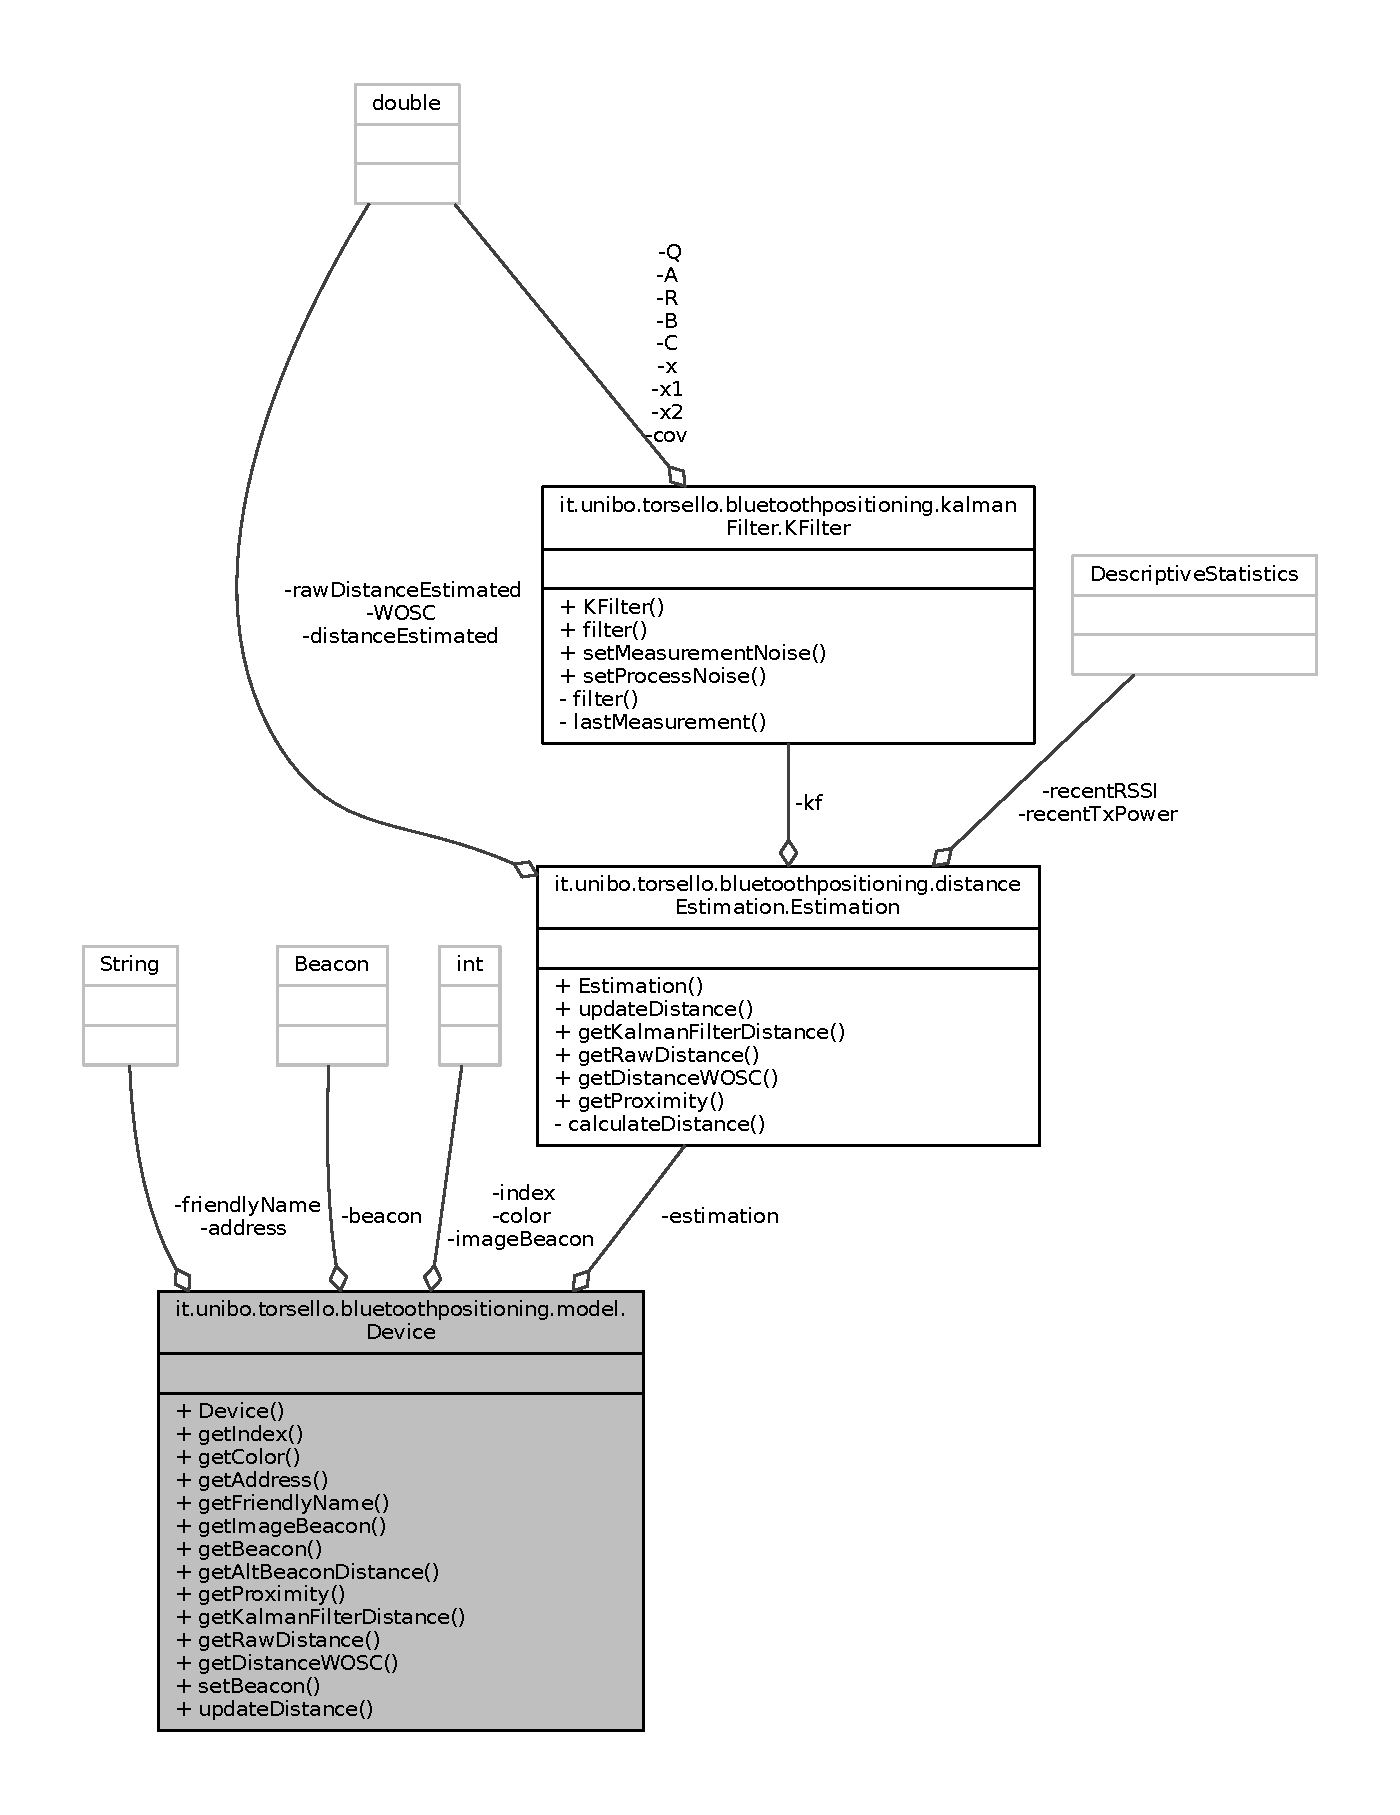
\includegraphics[width=350pt]{classit_1_1unibo_1_1torsello_1_1bluetoothpositioning_1_1model_1_1Device__coll__graph}
\end{center}
\end{figure}
\subsubsection*{Membri pubblici}
\begin{DoxyCompactItemize}
\item 
\hyperlink{classit_1_1unibo_1_1torsello_1_1bluetoothpositioning_1_1model_1_1Device_a2617f025dd33e0cae4adb3323245f865_a2617f025dd33e0cae4adb3323245f865}{Device} (int \hyperlink{classit_1_1unibo_1_1torsello_1_1bluetoothpositioning_1_1model_1_1Device_a55a01164b2388451f5e8344bfbc61ccc_a55a01164b2388451f5e8344bfbc61ccc}{index}, String \hyperlink{classit_1_1unibo_1_1torsello_1_1bluetoothpositioning_1_1model_1_1Device_a0abcf7e0df4ccc96e487c6f9b90b4e13_a0abcf7e0df4ccc96e487c6f9b90b4e13}{address}, String \hyperlink{classit_1_1unibo_1_1torsello_1_1bluetoothpositioning_1_1model_1_1Device_aa9a540b316c9de7f9b3a94f58570f6d3_aa9a540b316c9de7f9b3a94f58570f6d3}{friendly\+Name}, Integer \hyperlink{classit_1_1unibo_1_1torsello_1_1bluetoothpositioning_1_1model_1_1Device_aaba1f93e2a0f88f01262cb38a65489e6_aaba1f93e2a0f88f01262cb38a65489e6}{color}, Integer \hyperlink{classit_1_1unibo_1_1torsello_1_1bluetoothpositioning_1_1model_1_1Device_a2faee0d51162a4efebfc2db787901019_a2faee0d51162a4efebfc2db787901019}{image\+Beacon})
\item 
int \hyperlink{classit_1_1unibo_1_1torsello_1_1bluetoothpositioning_1_1model_1_1Device_a7f7e47588f721b360447d0f6ae2c4a9d_a7f7e47588f721b360447d0f6ae2c4a9d}{get\+Index} ()
\item 
Integer \hyperlink{classit_1_1unibo_1_1torsello_1_1bluetoothpositioning_1_1model_1_1Device_aad4f2885e5ed0279c7e0c6db684de5c3_aad4f2885e5ed0279c7e0c6db684de5c3}{get\+Color} ()
\item 
String \hyperlink{classit_1_1unibo_1_1torsello_1_1bluetoothpositioning_1_1model_1_1Device_ae4cd3fdda7414388cbda796f62543d5b_ae4cd3fdda7414388cbda796f62543d5b}{get\+Address} ()
\item 
String \hyperlink{classit_1_1unibo_1_1torsello_1_1bluetoothpositioning_1_1model_1_1Device_ab96e3e3bd6e9c9e27a42e619ca03ed71_ab96e3e3bd6e9c9e27a42e619ca03ed71}{get\+Friendly\+Name} ()
\item 
Integer \hyperlink{classit_1_1unibo_1_1torsello_1_1bluetoothpositioning_1_1model_1_1Device_a0fe04c6168a9a13bdf65eb0e5d407d37_a0fe04c6168a9a13bdf65eb0e5d407d37}{get\+Image\+Beacon} ()
\item 
Beacon \hyperlink{classit_1_1unibo_1_1torsello_1_1bluetoothpositioning_1_1model_1_1Device_a61b4951f3153550e8006f043eec034c2_a61b4951f3153550e8006f043eec034c2}{get\+Beacon} ()
\item 
double \hyperlink{classit_1_1unibo_1_1torsello_1_1bluetoothpositioning_1_1model_1_1Device_aa178afb829c0b5cae49af25e0e9b2117_aa178afb829c0b5cae49af25e0e9b2117}{get\+Alt\+Beacon\+Distance} ()
\item 
String \hyperlink{classit_1_1unibo_1_1torsello_1_1bluetoothpositioning_1_1model_1_1Device_a34510d139c99bc9cfba247ab6ff1b16f_a34510d139c99bc9cfba247ab6ff1b16f}{get\+Proximity} ()
\item 
double \hyperlink{classit_1_1unibo_1_1torsello_1_1bluetoothpositioning_1_1model_1_1Device_aa86454f965d50f015f1f40abe2d0d19a_aa86454f965d50f015f1f40abe2d0d19a}{get\+Kalman\+Filter\+Distance} ()
\item 
double \hyperlink{classit_1_1unibo_1_1torsello_1_1bluetoothpositioning_1_1model_1_1Device_abd5c0c1d478ac01c009959891456bbb8_abd5c0c1d478ac01c009959891456bbb8}{get\+Raw\+Distance} ()
\item 
double \hyperlink{classit_1_1unibo_1_1torsello_1_1bluetoothpositioning_1_1model_1_1Device_abcef7fbd06b5c97b412619a5b79b237c_abcef7fbd06b5c97b412619a5b79b237c}{get\+Distance\+W\+O\+SC} ()
\item 
void \hyperlink{classit_1_1unibo_1_1torsello_1_1bluetoothpositioning_1_1model_1_1Device_a7aff672e35f15a271dd93bd59e413f28_a7aff672e35f15a271dd93bd59e413f28}{set\+Beacon} (Beacon \hyperlink{classit_1_1unibo_1_1torsello_1_1bluetoothpositioning_1_1model_1_1Device_ad5ffce680eb2eb38fc6bb8aee234f155_ad5ffce680eb2eb38fc6bb8aee234f155}{beacon})
\item 
void \hyperlink{classit_1_1unibo_1_1torsello_1_1bluetoothpositioning_1_1model_1_1Device_af6e2efc8c50b88d07cc651db1f4bbb34_af6e2efc8c50b88d07cc651db1f4bbb34}{update\+Distance} (double process\+Noise)
\item 
boolean \hyperlink{classit_1_1unibo_1_1torsello_1_1bluetoothpositioning_1_1model_1_1Device_a7eb63440da744a389cc02d1d9a9b2421_a7eb63440da744a389cc02d1d9a9b2421}{is\+Kalman\+Filter\+Enabled} ()
\end{DoxyCompactItemize}
\subsubsection*{Attributi privati}
\begin{DoxyCompactItemize}
\item 
\hyperlink{classit_1_1unibo_1_1torsello_1_1bluetoothpositioning_1_1distanceEstimation_1_1Estimation}{Estimation} \hyperlink{classit_1_1unibo_1_1torsello_1_1bluetoothpositioning_1_1model_1_1Device_ac619c42728cd40f41a5f12fde56b4425_ac619c42728cd40f41a5f12fde56b4425}{estimation}
\item 
String \hyperlink{classit_1_1unibo_1_1torsello_1_1bluetoothpositioning_1_1model_1_1Device_a0abcf7e0df4ccc96e487c6f9b90b4e13_a0abcf7e0df4ccc96e487c6f9b90b4e13}{address}
\item 
String \hyperlink{classit_1_1unibo_1_1torsello_1_1bluetoothpositioning_1_1model_1_1Device_aa9a540b316c9de7f9b3a94f58570f6d3_aa9a540b316c9de7f9b3a94f58570f6d3}{friendly\+Name}
\item 
Beacon \hyperlink{classit_1_1unibo_1_1torsello_1_1bluetoothpositioning_1_1model_1_1Device_ad5ffce680eb2eb38fc6bb8aee234f155_ad5ffce680eb2eb38fc6bb8aee234f155}{beacon}
\item 
int \hyperlink{classit_1_1unibo_1_1torsello_1_1bluetoothpositioning_1_1model_1_1Device_a2faee0d51162a4efebfc2db787901019_a2faee0d51162a4efebfc2db787901019}{image\+Beacon}
\item 
int \hyperlink{classit_1_1unibo_1_1torsello_1_1bluetoothpositioning_1_1model_1_1Device_aaba1f93e2a0f88f01262cb38a65489e6_aaba1f93e2a0f88f01262cb38a65489e6}{color}
\item 
int \hyperlink{classit_1_1unibo_1_1torsello_1_1bluetoothpositioning_1_1model_1_1Device_a55a01164b2388451f5e8344bfbc61ccc_a55a01164b2388451f5e8344bfbc61ccc}{index}
\end{DoxyCompactItemize}


\subsubsection{Descrizione dettagliata}
Created by Federico Torsello. \href{mailto:federico.torsello@studio.unibo.it}{\tt federico.\+torsello@studio.\+unibo.\+it} 

\subsubsection{Documentazione dei costruttori e dei distruttori}
\hypertarget{classit_1_1unibo_1_1torsello_1_1bluetoothpositioning_1_1model_1_1Device_a2617f025dd33e0cae4adb3323245f865_a2617f025dd33e0cae4adb3323245f865}{}\label{classit_1_1unibo_1_1torsello_1_1bluetoothpositioning_1_1model_1_1Device_a2617f025dd33e0cae4adb3323245f865_a2617f025dd33e0cae4adb3323245f865} 
\index{it\+::unibo\+::torsello\+::bluetoothpositioning\+::model\+::\+Device@{it\+::unibo\+::torsello\+::bluetoothpositioning\+::model\+::\+Device}!Device@{Device}}
\index{Device@{Device}!it\+::unibo\+::torsello\+::bluetoothpositioning\+::model\+::\+Device@{it\+::unibo\+::torsello\+::bluetoothpositioning\+::model\+::\+Device}}
\paragraph{\texorpdfstring{Device()}{Device()}}
{\footnotesize\ttfamily it.\+unibo.\+torsello.\+bluetoothpositioning.\+model.\+Device.\+Device (\begin{DoxyParamCaption}\item[{int}]{index,  }\item[{String}]{address,  }\item[{String}]{friendly\+Name,  }\item[{Integer}]{color,  }\item[{Integer}]{image\+Beacon }\end{DoxyParamCaption})}


\begin{DoxyCode}
21                                                                                                       \{
22         this.\hyperlink{classit_1_1unibo_1_1torsello_1_1bluetoothpositioning_1_1model_1_1Device_a55a01164b2388451f5e8344bfbc61ccc_a55a01164b2388451f5e8344bfbc61ccc}{index} = \hyperlink{classit_1_1unibo_1_1torsello_1_1bluetoothpositioning_1_1model_1_1Device_a55a01164b2388451f5e8344bfbc61ccc_a55a01164b2388451f5e8344bfbc61ccc}{index};
23         this.\hyperlink{classit_1_1unibo_1_1torsello_1_1bluetoothpositioning_1_1model_1_1Device_a0abcf7e0df4ccc96e487c6f9b90b4e13_a0abcf7e0df4ccc96e487c6f9b90b4e13}{address} = \hyperlink{classit_1_1unibo_1_1torsello_1_1bluetoothpositioning_1_1model_1_1Device_a0abcf7e0df4ccc96e487c6f9b90b4e13_a0abcf7e0df4ccc96e487c6f9b90b4e13}{address};
24         this.\hyperlink{classit_1_1unibo_1_1torsello_1_1bluetoothpositioning_1_1model_1_1Device_aa9a540b316c9de7f9b3a94f58570f6d3_aa9a540b316c9de7f9b3a94f58570f6d3}{friendlyName} = \hyperlink{classit_1_1unibo_1_1torsello_1_1bluetoothpositioning_1_1model_1_1Device_aa9a540b316c9de7f9b3a94f58570f6d3_aa9a540b316c9de7f9b3a94f58570f6d3}{friendlyName};
25         this.\hyperlink{classit_1_1unibo_1_1torsello_1_1bluetoothpositioning_1_1model_1_1Device_ac619c42728cd40f41a5f12fde56b4425_ac619c42728cd40f41a5f12fde56b4425}{estimation} = \textcolor{keyword}{new} Estimation();
26         this.\hyperlink{classit_1_1unibo_1_1torsello_1_1bluetoothpositioning_1_1model_1_1Device_a2faee0d51162a4efebfc2db787901019_a2faee0d51162a4efebfc2db787901019}{imageBeacon} = \hyperlink{classit_1_1unibo_1_1torsello_1_1bluetoothpositioning_1_1model_1_1Device_a2faee0d51162a4efebfc2db787901019_a2faee0d51162a4efebfc2db787901019}{imageBeacon};
27         this.\hyperlink{classit_1_1unibo_1_1torsello_1_1bluetoothpositioning_1_1model_1_1Device_aaba1f93e2a0f88f01262cb38a65489e6_aaba1f93e2a0f88f01262cb38a65489e6}{color} = \hyperlink{classit_1_1unibo_1_1torsello_1_1bluetoothpositioning_1_1model_1_1Device_aaba1f93e2a0f88f01262cb38a65489e6_aaba1f93e2a0f88f01262cb38a65489e6}{color};
28     \}
\end{DoxyCode}


\subsubsection{Documentazione delle funzioni membro}
\hypertarget{classit_1_1unibo_1_1torsello_1_1bluetoothpositioning_1_1model_1_1Device_ae4cd3fdda7414388cbda796f62543d5b_ae4cd3fdda7414388cbda796f62543d5b}{}\label{classit_1_1unibo_1_1torsello_1_1bluetoothpositioning_1_1model_1_1Device_ae4cd3fdda7414388cbda796f62543d5b_ae4cd3fdda7414388cbda796f62543d5b} 
\index{it\+::unibo\+::torsello\+::bluetoothpositioning\+::model\+::\+Device@{it\+::unibo\+::torsello\+::bluetoothpositioning\+::model\+::\+Device}!get\+Address@{get\+Address}}
\index{get\+Address@{get\+Address}!it\+::unibo\+::torsello\+::bluetoothpositioning\+::model\+::\+Device@{it\+::unibo\+::torsello\+::bluetoothpositioning\+::model\+::\+Device}}
\paragraph{\texorpdfstring{get\+Address()}{getAddress()}}
{\footnotesize\ttfamily String it.\+unibo.\+torsello.\+bluetoothpositioning.\+model.\+Device.\+get\+Address (\begin{DoxyParamCaption}{ }\end{DoxyParamCaption})}


\begin{DoxyCode}
38                                \{
39         \textcolor{keywordflow}{return} this.\hyperlink{classit_1_1unibo_1_1torsello_1_1bluetoothpositioning_1_1model_1_1Device_a0abcf7e0df4ccc96e487c6f9b90b4e13_a0abcf7e0df4ccc96e487c6f9b90b4e13}{address};
40     \}
\end{DoxyCode}
\hypertarget{classit_1_1unibo_1_1torsello_1_1bluetoothpositioning_1_1model_1_1Device_aa178afb829c0b5cae49af25e0e9b2117_aa178afb829c0b5cae49af25e0e9b2117}{}\label{classit_1_1unibo_1_1torsello_1_1bluetoothpositioning_1_1model_1_1Device_aa178afb829c0b5cae49af25e0e9b2117_aa178afb829c0b5cae49af25e0e9b2117} 
\index{it\+::unibo\+::torsello\+::bluetoothpositioning\+::model\+::\+Device@{it\+::unibo\+::torsello\+::bluetoothpositioning\+::model\+::\+Device}!get\+Alt\+Beacon\+Distance@{get\+Alt\+Beacon\+Distance}}
\index{get\+Alt\+Beacon\+Distance@{get\+Alt\+Beacon\+Distance}!it\+::unibo\+::torsello\+::bluetoothpositioning\+::model\+::\+Device@{it\+::unibo\+::torsello\+::bluetoothpositioning\+::model\+::\+Device}}
\paragraph{\texorpdfstring{get\+Alt\+Beacon\+Distance()}{getAltBeaconDistance()}}
{\footnotesize\ttfamily double it.\+unibo.\+torsello.\+bluetoothpositioning.\+model.\+Device.\+get\+Alt\+Beacon\+Distance (\begin{DoxyParamCaption}{ }\end{DoxyParamCaption})}


\begin{DoxyCode}
54                                          \{
55         \textcolor{keywordflow}{return} \hyperlink{classit_1_1unibo_1_1torsello_1_1bluetoothpositioning_1_1model_1_1Device_ad5ffce680eb2eb38fc6bb8aee234f155_ad5ffce680eb2eb38fc6bb8aee234f155}{beacon}.getDistance();
56     \}
\end{DoxyCode}
\hypertarget{classit_1_1unibo_1_1torsello_1_1bluetoothpositioning_1_1model_1_1Device_a61b4951f3153550e8006f043eec034c2_a61b4951f3153550e8006f043eec034c2}{}\label{classit_1_1unibo_1_1torsello_1_1bluetoothpositioning_1_1model_1_1Device_a61b4951f3153550e8006f043eec034c2_a61b4951f3153550e8006f043eec034c2} 
\index{it\+::unibo\+::torsello\+::bluetoothpositioning\+::model\+::\+Device@{it\+::unibo\+::torsello\+::bluetoothpositioning\+::model\+::\+Device}!get\+Beacon@{get\+Beacon}}
\index{get\+Beacon@{get\+Beacon}!it\+::unibo\+::torsello\+::bluetoothpositioning\+::model\+::\+Device@{it\+::unibo\+::torsello\+::bluetoothpositioning\+::model\+::\+Device}}
\paragraph{\texorpdfstring{get\+Beacon()}{getBeacon()}}
{\footnotesize\ttfamily Beacon it.\+unibo.\+torsello.\+bluetoothpositioning.\+model.\+Device.\+get\+Beacon (\begin{DoxyParamCaption}{ }\end{DoxyParamCaption})}


\begin{DoxyCode}
50                               \{
51         \textcolor{keywordflow}{return} \hyperlink{classit_1_1unibo_1_1torsello_1_1bluetoothpositioning_1_1model_1_1Device_ad5ffce680eb2eb38fc6bb8aee234f155_ad5ffce680eb2eb38fc6bb8aee234f155}{beacon};
52     \}
\end{DoxyCode}
\hypertarget{classit_1_1unibo_1_1torsello_1_1bluetoothpositioning_1_1model_1_1Device_aad4f2885e5ed0279c7e0c6db684de5c3_aad4f2885e5ed0279c7e0c6db684de5c3}{}\label{classit_1_1unibo_1_1torsello_1_1bluetoothpositioning_1_1model_1_1Device_aad4f2885e5ed0279c7e0c6db684de5c3_aad4f2885e5ed0279c7e0c6db684de5c3} 
\index{it\+::unibo\+::torsello\+::bluetoothpositioning\+::model\+::\+Device@{it\+::unibo\+::torsello\+::bluetoothpositioning\+::model\+::\+Device}!get\+Color@{get\+Color}}
\index{get\+Color@{get\+Color}!it\+::unibo\+::torsello\+::bluetoothpositioning\+::model\+::\+Device@{it\+::unibo\+::torsello\+::bluetoothpositioning\+::model\+::\+Device}}
\paragraph{\texorpdfstring{get\+Color()}{getColor()}}
{\footnotesize\ttfamily Integer it.\+unibo.\+torsello.\+bluetoothpositioning.\+model.\+Device.\+get\+Color (\begin{DoxyParamCaption}{ }\end{DoxyParamCaption})}


\begin{DoxyCode}
34                               \{
35         \textcolor{keywordflow}{return} \hyperlink{classit_1_1unibo_1_1torsello_1_1bluetoothpositioning_1_1model_1_1Device_aaba1f93e2a0f88f01262cb38a65489e6_aaba1f93e2a0f88f01262cb38a65489e6}{color};
36     \}
\end{DoxyCode}
\hypertarget{classit_1_1unibo_1_1torsello_1_1bluetoothpositioning_1_1model_1_1Device_abcef7fbd06b5c97b412619a5b79b237c_abcef7fbd06b5c97b412619a5b79b237c}{}\label{classit_1_1unibo_1_1torsello_1_1bluetoothpositioning_1_1model_1_1Device_abcef7fbd06b5c97b412619a5b79b237c_abcef7fbd06b5c97b412619a5b79b237c} 
\index{it\+::unibo\+::torsello\+::bluetoothpositioning\+::model\+::\+Device@{it\+::unibo\+::torsello\+::bluetoothpositioning\+::model\+::\+Device}!get\+Distance\+W\+O\+SC@{get\+Distance\+W\+O\+SC}}
\index{get\+Distance\+W\+O\+SC@{get\+Distance\+W\+O\+SC}!it\+::unibo\+::torsello\+::bluetoothpositioning\+::model\+::\+Device@{it\+::unibo\+::torsello\+::bluetoothpositioning\+::model\+::\+Device}}
\paragraph{\texorpdfstring{get\+Distance\+W\+O\+S\+C()}{getDistanceWOSC()}}
{\footnotesize\ttfamily double it.\+unibo.\+torsello.\+bluetoothpositioning.\+model.\+Device.\+get\+Distance\+W\+O\+SC (\begin{DoxyParamCaption}{ }\end{DoxyParamCaption})}


\begin{DoxyCode}
75                                     \{
76         \textcolor{keywordflow}{return} \hyperlink{classit_1_1unibo_1_1torsello_1_1bluetoothpositioning_1_1model_1_1Device_ac619c42728cd40f41a5f12fde56b4425_ac619c42728cd40f41a5f12fde56b4425}{estimation}.\hyperlink{classit_1_1unibo_1_1torsello_1_1bluetoothpositioning_1_1distanceEstimation_1_1Estimation_a5c7bce21cd77c98a8d1e6df4c930397c_a5c7bce21cd77c98a8d1e6df4c930397c}{getDistanceWOSC}();
77     \}
\end{DoxyCode}
\hypertarget{classit_1_1unibo_1_1torsello_1_1bluetoothpositioning_1_1model_1_1Device_ab96e3e3bd6e9c9e27a42e619ca03ed71_ab96e3e3bd6e9c9e27a42e619ca03ed71}{}\label{classit_1_1unibo_1_1torsello_1_1bluetoothpositioning_1_1model_1_1Device_ab96e3e3bd6e9c9e27a42e619ca03ed71_ab96e3e3bd6e9c9e27a42e619ca03ed71} 
\index{it\+::unibo\+::torsello\+::bluetoothpositioning\+::model\+::\+Device@{it\+::unibo\+::torsello\+::bluetoothpositioning\+::model\+::\+Device}!get\+Friendly\+Name@{get\+Friendly\+Name}}
\index{get\+Friendly\+Name@{get\+Friendly\+Name}!it\+::unibo\+::torsello\+::bluetoothpositioning\+::model\+::\+Device@{it\+::unibo\+::torsello\+::bluetoothpositioning\+::model\+::\+Device}}
\paragraph{\texorpdfstring{get\+Friendly\+Name()}{getFriendlyName()}}
{\footnotesize\ttfamily String it.\+unibo.\+torsello.\+bluetoothpositioning.\+model.\+Device.\+get\+Friendly\+Name (\begin{DoxyParamCaption}{ }\end{DoxyParamCaption})}


\begin{DoxyCode}
42                                     \{
43         \textcolor{keywordflow}{return} \hyperlink{classit_1_1unibo_1_1torsello_1_1bluetoothpositioning_1_1model_1_1Device_aa9a540b316c9de7f9b3a94f58570f6d3_aa9a540b316c9de7f9b3a94f58570f6d3}{friendlyName};
44     \}
\end{DoxyCode}
\hypertarget{classit_1_1unibo_1_1torsello_1_1bluetoothpositioning_1_1model_1_1Device_a0fe04c6168a9a13bdf65eb0e5d407d37_a0fe04c6168a9a13bdf65eb0e5d407d37}{}\label{classit_1_1unibo_1_1torsello_1_1bluetoothpositioning_1_1model_1_1Device_a0fe04c6168a9a13bdf65eb0e5d407d37_a0fe04c6168a9a13bdf65eb0e5d407d37} 
\index{it\+::unibo\+::torsello\+::bluetoothpositioning\+::model\+::\+Device@{it\+::unibo\+::torsello\+::bluetoothpositioning\+::model\+::\+Device}!get\+Image\+Beacon@{get\+Image\+Beacon}}
\index{get\+Image\+Beacon@{get\+Image\+Beacon}!it\+::unibo\+::torsello\+::bluetoothpositioning\+::model\+::\+Device@{it\+::unibo\+::torsello\+::bluetoothpositioning\+::model\+::\+Device}}
\paragraph{\texorpdfstring{get\+Image\+Beacon()}{getImageBeacon()}}
{\footnotesize\ttfamily Integer it.\+unibo.\+torsello.\+bluetoothpositioning.\+model.\+Device.\+get\+Image\+Beacon (\begin{DoxyParamCaption}{ }\end{DoxyParamCaption})}


\begin{DoxyCode}
46                                     \{
47         \textcolor{keywordflow}{return} \hyperlink{classit_1_1unibo_1_1torsello_1_1bluetoothpositioning_1_1model_1_1Device_a2faee0d51162a4efebfc2db787901019_a2faee0d51162a4efebfc2db787901019}{imageBeacon};
48     \}
\end{DoxyCode}
\hypertarget{classit_1_1unibo_1_1torsello_1_1bluetoothpositioning_1_1model_1_1Device_a7f7e47588f721b360447d0f6ae2c4a9d_a7f7e47588f721b360447d0f6ae2c4a9d}{}\label{classit_1_1unibo_1_1torsello_1_1bluetoothpositioning_1_1model_1_1Device_a7f7e47588f721b360447d0f6ae2c4a9d_a7f7e47588f721b360447d0f6ae2c4a9d} 
\index{it\+::unibo\+::torsello\+::bluetoothpositioning\+::model\+::\+Device@{it\+::unibo\+::torsello\+::bluetoothpositioning\+::model\+::\+Device}!get\+Index@{get\+Index}}
\index{get\+Index@{get\+Index}!it\+::unibo\+::torsello\+::bluetoothpositioning\+::model\+::\+Device@{it\+::unibo\+::torsello\+::bluetoothpositioning\+::model\+::\+Device}}
\paragraph{\texorpdfstring{get\+Index()}{getIndex()}}
{\footnotesize\ttfamily int it.\+unibo.\+torsello.\+bluetoothpositioning.\+model.\+Device.\+get\+Index (\begin{DoxyParamCaption}{ }\end{DoxyParamCaption})}


\begin{DoxyCode}
30                           \{
31         \textcolor{keywordflow}{return} \hyperlink{classit_1_1unibo_1_1torsello_1_1bluetoothpositioning_1_1model_1_1Device_a55a01164b2388451f5e8344bfbc61ccc_a55a01164b2388451f5e8344bfbc61ccc}{index};
32     \}
\end{DoxyCode}
\hypertarget{classit_1_1unibo_1_1torsello_1_1bluetoothpositioning_1_1model_1_1Device_aa86454f965d50f015f1f40abe2d0d19a_aa86454f965d50f015f1f40abe2d0d19a}{}\label{classit_1_1unibo_1_1torsello_1_1bluetoothpositioning_1_1model_1_1Device_aa86454f965d50f015f1f40abe2d0d19a_aa86454f965d50f015f1f40abe2d0d19a} 
\index{it\+::unibo\+::torsello\+::bluetoothpositioning\+::model\+::\+Device@{it\+::unibo\+::torsello\+::bluetoothpositioning\+::model\+::\+Device}!get\+Kalman\+Filter\+Distance@{get\+Kalman\+Filter\+Distance}}
\index{get\+Kalman\+Filter\+Distance@{get\+Kalman\+Filter\+Distance}!it\+::unibo\+::torsello\+::bluetoothpositioning\+::model\+::\+Device@{it\+::unibo\+::torsello\+::bluetoothpositioning\+::model\+::\+Device}}
\paragraph{\texorpdfstring{get\+Kalman\+Filter\+Distance()}{getKalmanFilterDistance()}}
{\footnotesize\ttfamily double it.\+unibo.\+torsello.\+bluetoothpositioning.\+model.\+Device.\+get\+Kalman\+Filter\+Distance (\begin{DoxyParamCaption}{ }\end{DoxyParamCaption})}


\begin{DoxyCode}
63                                             \{
64         \textcolor{keywordflow}{if} (!\hyperlink{classit_1_1unibo_1_1torsello_1_1bluetoothpositioning_1_1model_1_1Device_ac619c42728cd40f41a5f12fde56b4425_ac619c42728cd40f41a5f12fde56b4425}{estimation}.\hyperlink{classit_1_1unibo_1_1torsello_1_1bluetoothpositioning_1_1distanceEstimation_1_1Estimation_a0863741935c878f7fa6f8c7c6cc086c9_a0863741935c878f7fa6f8c7c6cc086c9}{isKalmanFilterEnabled}())\{
65             \textcolor{keywordflow}{return} 0;
66         \}
67 
68         \textcolor{keywordflow}{return} \hyperlink{classit_1_1unibo_1_1torsello_1_1bluetoothpositioning_1_1model_1_1Device_ac619c42728cd40f41a5f12fde56b4425_ac619c42728cd40f41a5f12fde56b4425}{estimation}.\hyperlink{classit_1_1unibo_1_1torsello_1_1bluetoothpositioning_1_1distanceEstimation_1_1Estimation_a985e9b8b61c3d1e917a2e818b5f8b679_a985e9b8b61c3d1e917a2e818b5f8b679}{getKalmanFilterDistance}();
69     \}
\end{DoxyCode}
\hypertarget{classit_1_1unibo_1_1torsello_1_1bluetoothpositioning_1_1model_1_1Device_a34510d139c99bc9cfba247ab6ff1b16f_a34510d139c99bc9cfba247ab6ff1b16f}{}\label{classit_1_1unibo_1_1torsello_1_1bluetoothpositioning_1_1model_1_1Device_a34510d139c99bc9cfba247ab6ff1b16f_a34510d139c99bc9cfba247ab6ff1b16f} 
\index{it\+::unibo\+::torsello\+::bluetoothpositioning\+::model\+::\+Device@{it\+::unibo\+::torsello\+::bluetoothpositioning\+::model\+::\+Device}!get\+Proximity@{get\+Proximity}}
\index{get\+Proximity@{get\+Proximity}!it\+::unibo\+::torsello\+::bluetoothpositioning\+::model\+::\+Device@{it\+::unibo\+::torsello\+::bluetoothpositioning\+::model\+::\+Device}}
\paragraph{\texorpdfstring{get\+Proximity()}{getProximity()}}
{\footnotesize\ttfamily String it.\+unibo.\+torsello.\+bluetoothpositioning.\+model.\+Device.\+get\+Proximity (\begin{DoxyParamCaption}{ }\end{DoxyParamCaption})}


\begin{DoxyCode}
58                                  \{
59         \textcolor{keywordflow}{return} \hyperlink{classit_1_1unibo_1_1torsello_1_1bluetoothpositioning_1_1model_1_1Device_ac619c42728cd40f41a5f12fde56b4425_ac619c42728cd40f41a5f12fde56b4425}{estimation}.\hyperlink{classit_1_1unibo_1_1torsello_1_1bluetoothpositioning_1_1distanceEstimation_1_1Estimation_a2edfb9f301730647277474c61b41dbd5_a2edfb9f301730647277474c61b41dbd5}{getProximity}();
60     \}
\end{DoxyCode}
\hypertarget{classit_1_1unibo_1_1torsello_1_1bluetoothpositioning_1_1model_1_1Device_abd5c0c1d478ac01c009959891456bbb8_abd5c0c1d478ac01c009959891456bbb8}{}\label{classit_1_1unibo_1_1torsello_1_1bluetoothpositioning_1_1model_1_1Device_abd5c0c1d478ac01c009959891456bbb8_abd5c0c1d478ac01c009959891456bbb8} 
\index{it\+::unibo\+::torsello\+::bluetoothpositioning\+::model\+::\+Device@{it\+::unibo\+::torsello\+::bluetoothpositioning\+::model\+::\+Device}!get\+Raw\+Distance@{get\+Raw\+Distance}}
\index{get\+Raw\+Distance@{get\+Raw\+Distance}!it\+::unibo\+::torsello\+::bluetoothpositioning\+::model\+::\+Device@{it\+::unibo\+::torsello\+::bluetoothpositioning\+::model\+::\+Device}}
\paragraph{\texorpdfstring{get\+Raw\+Distance()}{getRawDistance()}}
{\footnotesize\ttfamily double it.\+unibo.\+torsello.\+bluetoothpositioning.\+model.\+Device.\+get\+Raw\+Distance (\begin{DoxyParamCaption}{ }\end{DoxyParamCaption})}


\begin{DoxyCode}
71                                    \{
72         \textcolor{keywordflow}{return} \hyperlink{classit_1_1unibo_1_1torsello_1_1bluetoothpositioning_1_1model_1_1Device_ac619c42728cd40f41a5f12fde56b4425_ac619c42728cd40f41a5f12fde56b4425}{estimation}.\hyperlink{classit_1_1unibo_1_1torsello_1_1bluetoothpositioning_1_1distanceEstimation_1_1Estimation_ad355b2e850a8d6013ef771eecd740e1b_ad355b2e850a8d6013ef771eecd740e1b}{getRawDistance}();
73     \}
\end{DoxyCode}
\hypertarget{classit_1_1unibo_1_1torsello_1_1bluetoothpositioning_1_1model_1_1Device_a7eb63440da744a389cc02d1d9a9b2421_a7eb63440da744a389cc02d1d9a9b2421}{}\label{classit_1_1unibo_1_1torsello_1_1bluetoothpositioning_1_1model_1_1Device_a7eb63440da744a389cc02d1d9a9b2421_a7eb63440da744a389cc02d1d9a9b2421} 
\index{it\+::unibo\+::torsello\+::bluetoothpositioning\+::model\+::\+Device@{it\+::unibo\+::torsello\+::bluetoothpositioning\+::model\+::\+Device}!is\+Kalman\+Filter\+Enabled@{is\+Kalman\+Filter\+Enabled}}
\index{is\+Kalman\+Filter\+Enabled@{is\+Kalman\+Filter\+Enabled}!it\+::unibo\+::torsello\+::bluetoothpositioning\+::model\+::\+Device@{it\+::unibo\+::torsello\+::bluetoothpositioning\+::model\+::\+Device}}
\paragraph{\texorpdfstring{is\+Kalman\+Filter\+Enabled()}{isKalmanFilterEnabled()}}
{\footnotesize\ttfamily boolean it.\+unibo.\+torsello.\+bluetoothpositioning.\+model.\+Device.\+is\+Kalman\+Filter\+Enabled (\begin{DoxyParamCaption}{ }\end{DoxyParamCaption})}


\begin{DoxyCode}
89                                           \{
90         \textcolor{keywordflow}{return} \hyperlink{classit_1_1unibo_1_1torsello_1_1bluetoothpositioning_1_1model_1_1Device_ac619c42728cd40f41a5f12fde56b4425_ac619c42728cd40f41a5f12fde56b4425}{estimation}.\hyperlink{classit_1_1unibo_1_1torsello_1_1bluetoothpositioning_1_1distanceEstimation_1_1Estimation_a0863741935c878f7fa6f8c7c6cc086c9_a0863741935c878f7fa6f8c7c6cc086c9}{isKalmanFilterEnabled}();
91     \}
\end{DoxyCode}
\hypertarget{classit_1_1unibo_1_1torsello_1_1bluetoothpositioning_1_1model_1_1Device_a7aff672e35f15a271dd93bd59e413f28_a7aff672e35f15a271dd93bd59e413f28}{}\label{classit_1_1unibo_1_1torsello_1_1bluetoothpositioning_1_1model_1_1Device_a7aff672e35f15a271dd93bd59e413f28_a7aff672e35f15a271dd93bd59e413f28} 
\index{it\+::unibo\+::torsello\+::bluetoothpositioning\+::model\+::\+Device@{it\+::unibo\+::torsello\+::bluetoothpositioning\+::model\+::\+Device}!set\+Beacon@{set\+Beacon}}
\index{set\+Beacon@{set\+Beacon}!it\+::unibo\+::torsello\+::bluetoothpositioning\+::model\+::\+Device@{it\+::unibo\+::torsello\+::bluetoothpositioning\+::model\+::\+Device}}
\paragraph{\texorpdfstring{set\+Beacon()}{setBeacon()}}
{\footnotesize\ttfamily void it.\+unibo.\+torsello.\+bluetoothpositioning.\+model.\+Device.\+set\+Beacon (\begin{DoxyParamCaption}\item[{Beacon}]{beacon }\end{DoxyParamCaption})}


\begin{DoxyCode}
79                                          \{
80         this.\hyperlink{classit_1_1unibo_1_1torsello_1_1bluetoothpositioning_1_1model_1_1Device_ad5ffce680eb2eb38fc6bb8aee234f155_ad5ffce680eb2eb38fc6bb8aee234f155}{beacon} = \hyperlink{classit_1_1unibo_1_1torsello_1_1bluetoothpositioning_1_1model_1_1Device_ad5ffce680eb2eb38fc6bb8aee234f155_ad5ffce680eb2eb38fc6bb8aee234f155}{beacon};
81     \}
\end{DoxyCode}
\hypertarget{classit_1_1unibo_1_1torsello_1_1bluetoothpositioning_1_1model_1_1Device_af6e2efc8c50b88d07cc651db1f4bbb34_af6e2efc8c50b88d07cc651db1f4bbb34}{}\label{classit_1_1unibo_1_1torsello_1_1bluetoothpositioning_1_1model_1_1Device_af6e2efc8c50b88d07cc651db1f4bbb34_af6e2efc8c50b88d07cc651db1f4bbb34} 
\index{it\+::unibo\+::torsello\+::bluetoothpositioning\+::model\+::\+Device@{it\+::unibo\+::torsello\+::bluetoothpositioning\+::model\+::\+Device}!update\+Distance@{update\+Distance}}
\index{update\+Distance@{update\+Distance}!it\+::unibo\+::torsello\+::bluetoothpositioning\+::model\+::\+Device@{it\+::unibo\+::torsello\+::bluetoothpositioning\+::model\+::\+Device}}
\paragraph{\texorpdfstring{update\+Distance()}{updateDistance()}}
{\footnotesize\ttfamily void it.\+unibo.\+torsello.\+bluetoothpositioning.\+model.\+Device.\+update\+Distance (\begin{DoxyParamCaption}\item[{double}]{process\+Noise }\end{DoxyParamCaption})}


\begin{DoxyCode}
83                                                     \{
84         \textcolor{keywordflow}{if} (\hyperlink{classit_1_1unibo_1_1torsello_1_1bluetoothpositioning_1_1model_1_1Device_ad5ffce680eb2eb38fc6bb8aee234f155_ad5ffce680eb2eb38fc6bb8aee234f155}{beacon} != null) \{
85             \hyperlink{classit_1_1unibo_1_1torsello_1_1bluetoothpositioning_1_1model_1_1Device_ac619c42728cd40f41a5f12fde56b4425_ac619c42728cd40f41a5f12fde56b4425}{estimation}.\hyperlink{classit_1_1unibo_1_1torsello_1_1bluetoothpositioning_1_1distanceEstimation_1_1Estimation_aaf86439861db7facf3f5338ec2fc6cde_aaf86439861db7facf3f5338ec2fc6cde}{updateDistance}(\hyperlink{classit_1_1unibo_1_1torsello_1_1bluetoothpositioning_1_1model_1_1Device_ad5ffce680eb2eb38fc6bb8aee234f155_ad5ffce680eb2eb38fc6bb8aee234f155}{beacon}, processNoise);
86         \}
87     \}
\end{DoxyCode}


\subsubsection{Documentazione dei membri dato}
\hypertarget{classit_1_1unibo_1_1torsello_1_1bluetoothpositioning_1_1model_1_1Device_a0abcf7e0df4ccc96e487c6f9b90b4e13_a0abcf7e0df4ccc96e487c6f9b90b4e13}{}\label{classit_1_1unibo_1_1torsello_1_1bluetoothpositioning_1_1model_1_1Device_a0abcf7e0df4ccc96e487c6f9b90b4e13_a0abcf7e0df4ccc96e487c6f9b90b4e13} 
\index{it\+::unibo\+::torsello\+::bluetoothpositioning\+::model\+::\+Device@{it\+::unibo\+::torsello\+::bluetoothpositioning\+::model\+::\+Device}!address@{address}}
\index{address@{address}!it\+::unibo\+::torsello\+::bluetoothpositioning\+::model\+::\+Device@{it\+::unibo\+::torsello\+::bluetoothpositioning\+::model\+::\+Device}}
\paragraph{\texorpdfstring{address}{address}}
{\footnotesize\ttfamily String it.\+unibo.\+torsello.\+bluetoothpositioning.\+model.\+Device.\+address\hspace{0.3cm}{\ttfamily [private]}}

\hypertarget{classit_1_1unibo_1_1torsello_1_1bluetoothpositioning_1_1model_1_1Device_ad5ffce680eb2eb38fc6bb8aee234f155_ad5ffce680eb2eb38fc6bb8aee234f155}{}\label{classit_1_1unibo_1_1torsello_1_1bluetoothpositioning_1_1model_1_1Device_ad5ffce680eb2eb38fc6bb8aee234f155_ad5ffce680eb2eb38fc6bb8aee234f155} 
\index{it\+::unibo\+::torsello\+::bluetoothpositioning\+::model\+::\+Device@{it\+::unibo\+::torsello\+::bluetoothpositioning\+::model\+::\+Device}!beacon@{beacon}}
\index{beacon@{beacon}!it\+::unibo\+::torsello\+::bluetoothpositioning\+::model\+::\+Device@{it\+::unibo\+::torsello\+::bluetoothpositioning\+::model\+::\+Device}}
\paragraph{\texorpdfstring{beacon}{beacon}}
{\footnotesize\ttfamily Beacon it.\+unibo.\+torsello.\+bluetoothpositioning.\+model.\+Device.\+beacon\hspace{0.3cm}{\ttfamily [private]}}

\hypertarget{classit_1_1unibo_1_1torsello_1_1bluetoothpositioning_1_1model_1_1Device_aaba1f93e2a0f88f01262cb38a65489e6_aaba1f93e2a0f88f01262cb38a65489e6}{}\label{classit_1_1unibo_1_1torsello_1_1bluetoothpositioning_1_1model_1_1Device_aaba1f93e2a0f88f01262cb38a65489e6_aaba1f93e2a0f88f01262cb38a65489e6} 
\index{it\+::unibo\+::torsello\+::bluetoothpositioning\+::model\+::\+Device@{it\+::unibo\+::torsello\+::bluetoothpositioning\+::model\+::\+Device}!color@{color}}
\index{color@{color}!it\+::unibo\+::torsello\+::bluetoothpositioning\+::model\+::\+Device@{it\+::unibo\+::torsello\+::bluetoothpositioning\+::model\+::\+Device}}
\paragraph{\texorpdfstring{color}{color}}
{\footnotesize\ttfamily int it.\+unibo.\+torsello.\+bluetoothpositioning.\+model.\+Device.\+color\hspace{0.3cm}{\ttfamily [private]}}

\hypertarget{classit_1_1unibo_1_1torsello_1_1bluetoothpositioning_1_1model_1_1Device_ac619c42728cd40f41a5f12fde56b4425_ac619c42728cd40f41a5f12fde56b4425}{}\label{classit_1_1unibo_1_1torsello_1_1bluetoothpositioning_1_1model_1_1Device_ac619c42728cd40f41a5f12fde56b4425_ac619c42728cd40f41a5f12fde56b4425} 
\index{it\+::unibo\+::torsello\+::bluetoothpositioning\+::model\+::\+Device@{it\+::unibo\+::torsello\+::bluetoothpositioning\+::model\+::\+Device}!estimation@{estimation}}
\index{estimation@{estimation}!it\+::unibo\+::torsello\+::bluetoothpositioning\+::model\+::\+Device@{it\+::unibo\+::torsello\+::bluetoothpositioning\+::model\+::\+Device}}
\paragraph{\texorpdfstring{estimation}{estimation}}
{\footnotesize\ttfamily \hyperlink{classit_1_1unibo_1_1torsello_1_1bluetoothpositioning_1_1distanceEstimation_1_1Estimation}{Estimation} it.\+unibo.\+torsello.\+bluetoothpositioning.\+model.\+Device.\+estimation\hspace{0.3cm}{\ttfamily [private]}}

\hypertarget{classit_1_1unibo_1_1torsello_1_1bluetoothpositioning_1_1model_1_1Device_aa9a540b316c9de7f9b3a94f58570f6d3_aa9a540b316c9de7f9b3a94f58570f6d3}{}\label{classit_1_1unibo_1_1torsello_1_1bluetoothpositioning_1_1model_1_1Device_aa9a540b316c9de7f9b3a94f58570f6d3_aa9a540b316c9de7f9b3a94f58570f6d3} 
\index{it\+::unibo\+::torsello\+::bluetoothpositioning\+::model\+::\+Device@{it\+::unibo\+::torsello\+::bluetoothpositioning\+::model\+::\+Device}!friendly\+Name@{friendly\+Name}}
\index{friendly\+Name@{friendly\+Name}!it\+::unibo\+::torsello\+::bluetoothpositioning\+::model\+::\+Device@{it\+::unibo\+::torsello\+::bluetoothpositioning\+::model\+::\+Device}}
\paragraph{\texorpdfstring{friendly\+Name}{friendlyName}}
{\footnotesize\ttfamily String it.\+unibo.\+torsello.\+bluetoothpositioning.\+model.\+Device.\+friendly\+Name\hspace{0.3cm}{\ttfamily [private]}}

\hypertarget{classit_1_1unibo_1_1torsello_1_1bluetoothpositioning_1_1model_1_1Device_a2faee0d51162a4efebfc2db787901019_a2faee0d51162a4efebfc2db787901019}{}\label{classit_1_1unibo_1_1torsello_1_1bluetoothpositioning_1_1model_1_1Device_a2faee0d51162a4efebfc2db787901019_a2faee0d51162a4efebfc2db787901019} 
\index{it\+::unibo\+::torsello\+::bluetoothpositioning\+::model\+::\+Device@{it\+::unibo\+::torsello\+::bluetoothpositioning\+::model\+::\+Device}!image\+Beacon@{image\+Beacon}}
\index{image\+Beacon@{image\+Beacon}!it\+::unibo\+::torsello\+::bluetoothpositioning\+::model\+::\+Device@{it\+::unibo\+::torsello\+::bluetoothpositioning\+::model\+::\+Device}}
\paragraph{\texorpdfstring{image\+Beacon}{imageBeacon}}
{\footnotesize\ttfamily int it.\+unibo.\+torsello.\+bluetoothpositioning.\+model.\+Device.\+image\+Beacon\hspace{0.3cm}{\ttfamily [private]}}

\hypertarget{classit_1_1unibo_1_1torsello_1_1bluetoothpositioning_1_1model_1_1Device_a55a01164b2388451f5e8344bfbc61ccc_a55a01164b2388451f5e8344bfbc61ccc}{}\label{classit_1_1unibo_1_1torsello_1_1bluetoothpositioning_1_1model_1_1Device_a55a01164b2388451f5e8344bfbc61ccc_a55a01164b2388451f5e8344bfbc61ccc} 
\index{it\+::unibo\+::torsello\+::bluetoothpositioning\+::model\+::\+Device@{it\+::unibo\+::torsello\+::bluetoothpositioning\+::model\+::\+Device}!index@{index}}
\index{index@{index}!it\+::unibo\+::torsello\+::bluetoothpositioning\+::model\+::\+Device@{it\+::unibo\+::torsello\+::bluetoothpositioning\+::model\+::\+Device}}
\paragraph{\texorpdfstring{index}{index}}
{\footnotesize\ttfamily int it.\+unibo.\+torsello.\+bluetoothpositioning.\+model.\+Device.\+index\hspace{0.3cm}{\ttfamily [private]}}



La documentazione per questa classe è stata generata a partire dal seguente file\+:\begin{DoxyCompactItemize}
\item 
\hyperlink{Device_8java}{Device.\+java}\end{DoxyCompactItemize}

\hypertarget{classit_1_1unibo_1_1torsello_1_1bluetoothpositioning_1_1adapter_1_1DeviceCardViewAdapter}{}\subsection{Riferimenti per la classe it.\+unibo.\+torsello.\+bluetoothpositioning.\+adapter.\+Device\+Card\+View\+Adapter}
\label{classit_1_1unibo_1_1torsello_1_1bluetoothpositioning_1_1adapter_1_1DeviceCardViewAdapter}\index{it.\+unibo.\+torsello.\+bluetoothpositioning.\+adapter.\+Device\+Card\+View\+Adapter@{it.\+unibo.\+torsello.\+bluetoothpositioning.\+adapter.\+Device\+Card\+View\+Adapter}}


Diagramma delle classi per it.\+unibo.\+torsello.\+bluetoothpositioning.\+adapter.\+Device\+Card\+View\+Adapter
\nopagebreak
\begin{figure}[H]
\begin{center}
\leavevmode
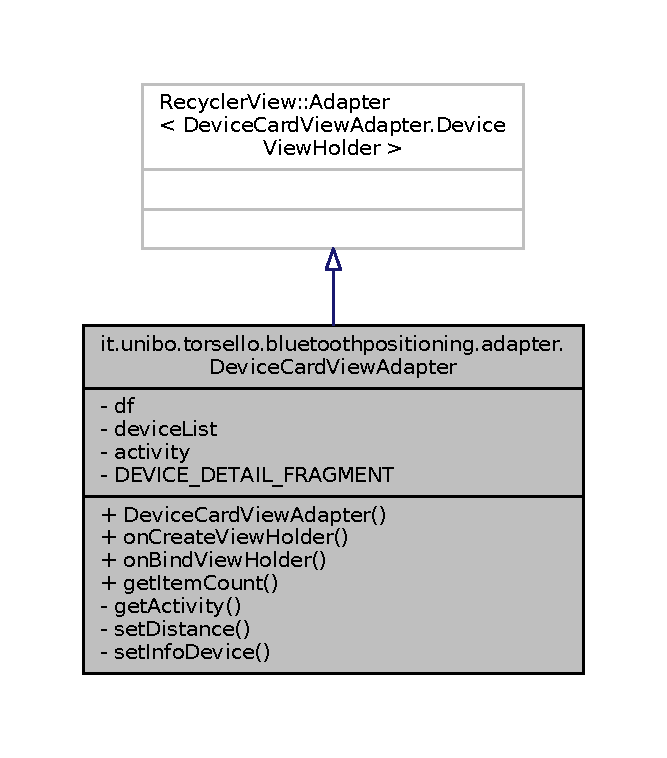
\includegraphics[width=320pt]{classit_1_1unibo_1_1torsello_1_1bluetoothpositioning_1_1adapter_1_1DeviceCardViewAdapter__inherit__graph}
\end{center}
\end{figure}


Diagramma di collaborazione per it.\+unibo.\+torsello.\+bluetoothpositioning.\+adapter.\+Device\+Card\+View\+Adapter\+:
\nopagebreak
\begin{figure}[H]
\begin{center}
\leavevmode
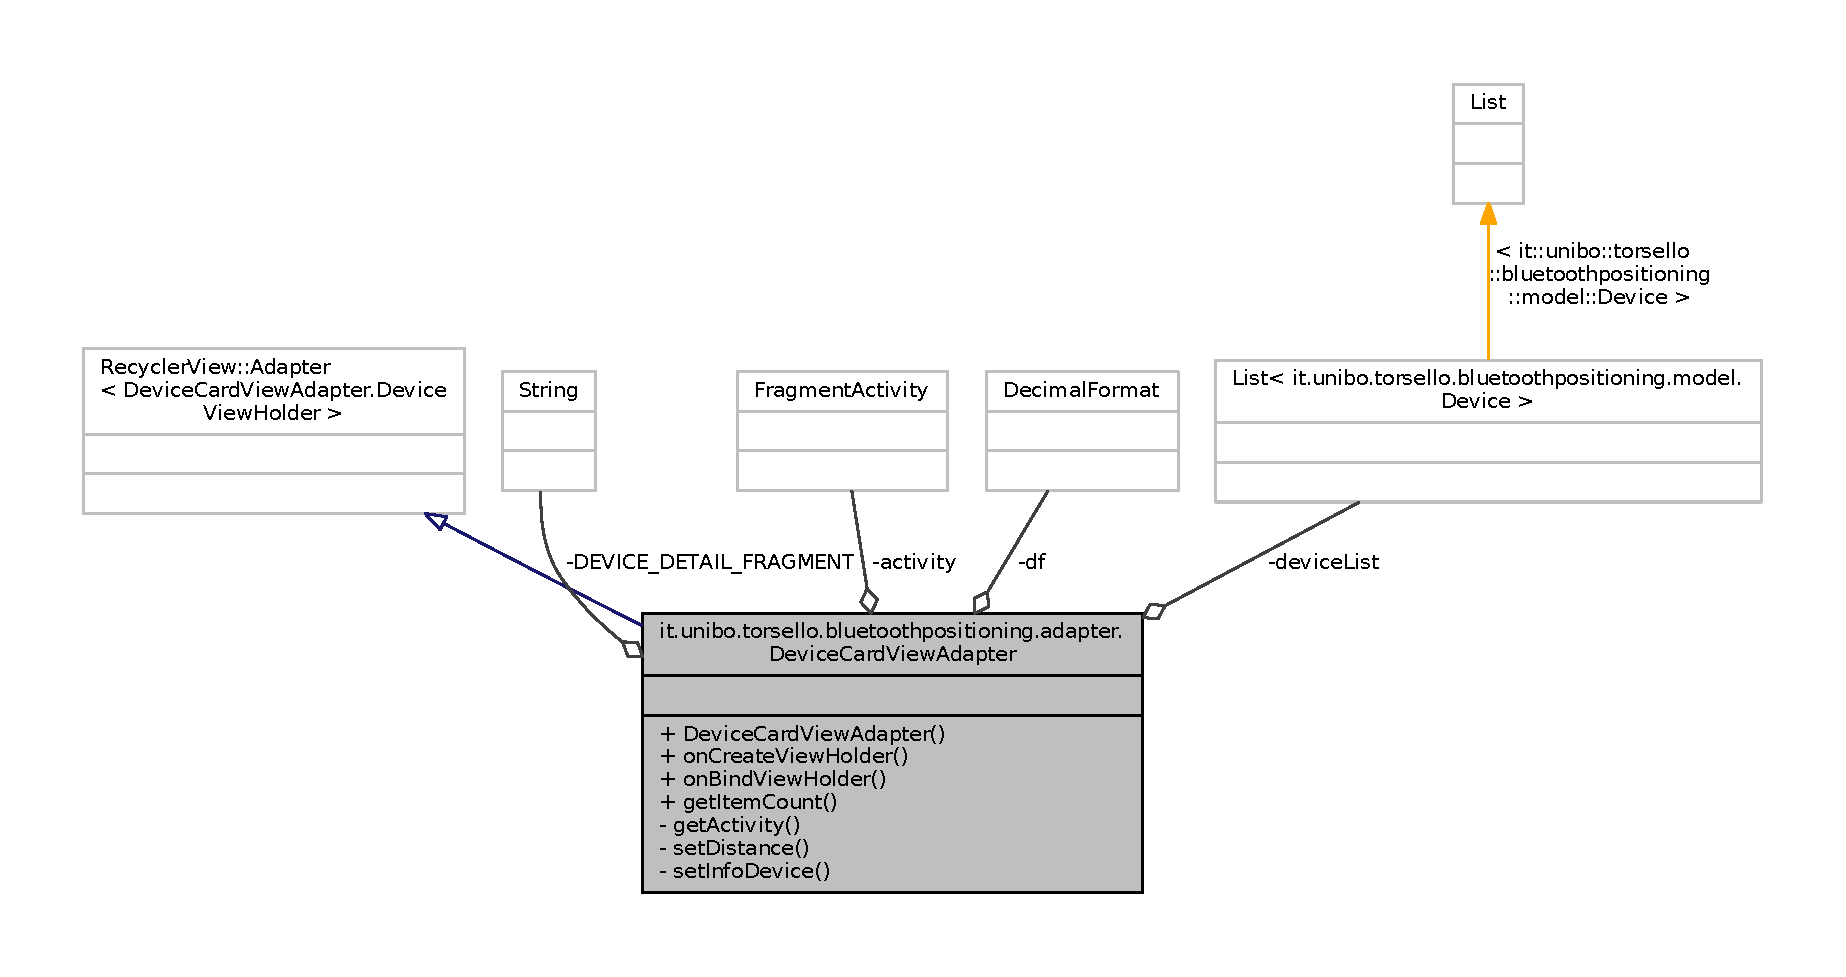
\includegraphics[width=350pt]{classit_1_1unibo_1_1torsello_1_1bluetoothpositioning_1_1adapter_1_1DeviceCardViewAdapter__coll__graph}
\end{center}
\end{figure}
\subsubsection*{Composti}
\begin{DoxyCompactItemize}
\item 
class \hyperlink{classit_1_1unibo_1_1torsello_1_1bluetoothpositioning_1_1adapter_1_1DeviceCardViewAdapter_1_1DeviceViewHolder}{Device\+View\+Holder}
\end{DoxyCompactItemize}
\subsubsection*{Membri pubblici}
\begin{DoxyCompactItemize}
\item 
\hyperlink{classit_1_1unibo_1_1torsello_1_1bluetoothpositioning_1_1adapter_1_1DeviceCardViewAdapter_a5f15271cd20868ac66c3c0876adca536_a5f15271cd20868ac66c3c0876adca536}{Device\+Card\+View\+Adapter} (final Fragment\+Activity fragment\+Activity, List$<$ \hyperlink{classit_1_1unibo_1_1torsello_1_1bluetoothpositioning_1_1model_1_1Device}{Device} $>$ \hyperlink{classit_1_1unibo_1_1torsello_1_1bluetoothpositioning_1_1adapter_1_1DeviceCardViewAdapter_a72413f87c723c585bd1ad9bc5711cf39_a72413f87c723c585bd1ad9bc5711cf39}{device\+List})
\item 
\hyperlink{classit_1_1unibo_1_1torsello_1_1bluetoothpositioning_1_1adapter_1_1DeviceCardViewAdapter_1_1DeviceViewHolder}{Device\+View\+Holder} \hyperlink{classit_1_1unibo_1_1torsello_1_1bluetoothpositioning_1_1adapter_1_1DeviceCardViewAdapter_a41227667123e30333d534b562a889229_a41227667123e30333d534b562a889229}{on\+Create\+View\+Holder} (View\+Group parent, int view\+Type)
\item 
void \hyperlink{classit_1_1unibo_1_1torsello_1_1bluetoothpositioning_1_1adapter_1_1DeviceCardViewAdapter_a3785bbe8696e1af4d8fb24e7058aa413_a3785bbe8696e1af4d8fb24e7058aa413}{on\+Bind\+View\+Holder} (\hyperlink{classit_1_1unibo_1_1torsello_1_1bluetoothpositioning_1_1adapter_1_1DeviceCardViewAdapter_1_1DeviceViewHolder}{Device\+View\+Holder} holder, final int position)
\item 
int \hyperlink{classit_1_1unibo_1_1torsello_1_1bluetoothpositioning_1_1adapter_1_1DeviceCardViewAdapter_ac039d50f397db6d5af06ca534e3e59a9_ac039d50f397db6d5af06ca534e3e59a9}{get\+Item\+Count} ()
\end{DoxyCompactItemize}
\subsubsection*{Membri privati}
\begin{DoxyCompactItemize}
\item 
Fragment\+Activity \hyperlink{classit_1_1unibo_1_1torsello_1_1bluetoothpositioning_1_1adapter_1_1DeviceCardViewAdapter_a0ff32c6bf5d84b68021bf586d64cacaf_a0ff32c6bf5d84b68021bf586d64cacaf}{get\+Activity} ()
\item 
void \hyperlink{classit_1_1unibo_1_1torsello_1_1bluetoothpositioning_1_1adapter_1_1DeviceCardViewAdapter_a8d5baa2d386a92ba4fb20b71e6e517f9_a8d5baa2d386a92ba4fb20b71e6e517f9}{set\+Distance} (\hyperlink{classit_1_1unibo_1_1torsello_1_1bluetoothpositioning_1_1adapter_1_1DeviceCardViewAdapter_1_1DeviceViewHolder}{Device\+View\+Holder} holder, \hyperlink{classit_1_1unibo_1_1torsello_1_1bluetoothpositioning_1_1model_1_1Device}{Device} device)
\item 
void \hyperlink{classit_1_1unibo_1_1torsello_1_1bluetoothpositioning_1_1adapter_1_1DeviceCardViewAdapter_aa43ee1f594b3489f6e9e4b8e20ea1612_aa43ee1f594b3489f6e9e4b8e20ea1612}{set\+Info\+Device} (\hyperlink{classit_1_1unibo_1_1torsello_1_1bluetoothpositioning_1_1adapter_1_1DeviceCardViewAdapter_1_1DeviceViewHolder}{Device\+View\+Holder} holder, Beacon beacon)
\end{DoxyCompactItemize}
\subsubsection*{Attributi privati}
\begin{DoxyCompactItemize}
\item 
Decimal\+Format \hyperlink{classit_1_1unibo_1_1torsello_1_1bluetoothpositioning_1_1adapter_1_1DeviceCardViewAdapter_ae3a2fe6b4e69e1f9b8edfb9bcba14057_ae3a2fe6b4e69e1f9b8edfb9bcba14057}{df}
\item 
List$<$ \hyperlink{classit_1_1unibo_1_1torsello_1_1bluetoothpositioning_1_1model_1_1Device}{Device} $>$ \hyperlink{classit_1_1unibo_1_1torsello_1_1bluetoothpositioning_1_1adapter_1_1DeviceCardViewAdapter_a72413f87c723c585bd1ad9bc5711cf39_a72413f87c723c585bd1ad9bc5711cf39}{device\+List}
\item 
Fragment\+Activity \hyperlink{classit_1_1unibo_1_1torsello_1_1bluetoothpositioning_1_1adapter_1_1DeviceCardViewAdapter_ad9b0572ad094da8225f1c2024ac2eb61_ad9b0572ad094da8225f1c2024ac2eb61}{activity}
\end{DoxyCompactItemize}
\subsubsection*{Attributi privati statici}
\begin{DoxyCompactItemize}
\item 
static final String \hyperlink{classit_1_1unibo_1_1torsello_1_1bluetoothpositioning_1_1adapter_1_1DeviceCardViewAdapter_a0d362081de4afb44abc82197aa597a18_a0d362081de4afb44abc82197aa597a18}{D\+E\+V\+I\+C\+E\+\_\+\+D\+E\+T\+A\+I\+L\+\_\+\+F\+R\+A\+G\+M\+E\+NT} = \char`\"{}device detail\char`\"{}
\end{DoxyCompactItemize}


\subsubsection{Descrizione dettagliata}
Created by Federico Torsello. \href{mailto:federico.torsello@studio.unibo.it}{\tt federico.\+torsello@studio.\+unibo.\+it} 

\subsubsection{Documentazione dei costruttori e dei distruttori}
\hypertarget{classit_1_1unibo_1_1torsello_1_1bluetoothpositioning_1_1adapter_1_1DeviceCardViewAdapter_a5f15271cd20868ac66c3c0876adca536_a5f15271cd20868ac66c3c0876adca536}{}\label{classit_1_1unibo_1_1torsello_1_1bluetoothpositioning_1_1adapter_1_1DeviceCardViewAdapter_a5f15271cd20868ac66c3c0876adca536_a5f15271cd20868ac66c3c0876adca536} 
\index{it\+::unibo\+::torsello\+::bluetoothpositioning\+::adapter\+::\+Device\+Card\+View\+Adapter@{it\+::unibo\+::torsello\+::bluetoothpositioning\+::adapter\+::\+Device\+Card\+View\+Adapter}!Device\+Card\+View\+Adapter@{Device\+Card\+View\+Adapter}}
\index{Device\+Card\+View\+Adapter@{Device\+Card\+View\+Adapter}!it\+::unibo\+::torsello\+::bluetoothpositioning\+::adapter\+::\+Device\+Card\+View\+Adapter@{it\+::unibo\+::torsello\+::bluetoothpositioning\+::adapter\+::\+Device\+Card\+View\+Adapter}}
\paragraph{\texorpdfstring{Device\+Card\+View\+Adapter()}{DeviceCardViewAdapter()}}
{\footnotesize\ttfamily it.\+unibo.\+torsello.\+bluetoothpositioning.\+adapter.\+Device\+Card\+View\+Adapter.\+Device\+Card\+View\+Adapter (\begin{DoxyParamCaption}\item[{final Fragment\+Activity}]{fragment\+Activity,  }\item[{List$<$ \hyperlink{classit_1_1unibo_1_1torsello_1_1bluetoothpositioning_1_1model_1_1Device}{Device} $>$}]{device\+List }\end{DoxyParamCaption})}


\begin{DoxyCode}
38                                                                                                    \{
39 
40         this.\hyperlink{classit_1_1unibo_1_1torsello_1_1bluetoothpositioning_1_1adapter_1_1DeviceCardViewAdapter_a72413f87c723c585bd1ad9bc5711cf39_a72413f87c723c585bd1ad9bc5711cf39}{deviceList} = \textcolor{keyword}{new} ArrayList<>();
41         this.\hyperlink{classit_1_1unibo_1_1torsello_1_1bluetoothpositioning_1_1adapter_1_1DeviceCardViewAdapter_a72413f87c723c585bd1ad9bc5711cf39_a72413f87c723c585bd1ad9bc5711cf39}{deviceList} = \hyperlink{classit_1_1unibo_1_1torsello_1_1bluetoothpositioning_1_1adapter_1_1DeviceCardViewAdapter_a72413f87c723c585bd1ad9bc5711cf39_a72413f87c723c585bd1ad9bc5711cf39}{deviceList};
42         this.\hyperlink{classit_1_1unibo_1_1torsello_1_1bluetoothpositioning_1_1adapter_1_1DeviceCardViewAdapter_ad9b0572ad094da8225f1c2024ac2eb61_ad9b0572ad094da8225f1c2024ac2eb61}{activity} = fragmentActivity;
43 
44         \hyperlink{classit_1_1unibo_1_1torsello_1_1bluetoothpositioning_1_1adapter_1_1DeviceCardViewAdapter_ae3a2fe6b4e69e1f9b8edfb9bcba14057_ae3a2fe6b4e69e1f9b8edfb9bcba14057}{df} = \textcolor{keyword}{new} DecimalFormat(\textcolor{stringliteral}{"0.00"}, DecimalFormatSymbols.getInstance());
45     \}
\end{DoxyCode}


\subsubsection{Documentazione delle funzioni membro}
\hypertarget{classit_1_1unibo_1_1torsello_1_1bluetoothpositioning_1_1adapter_1_1DeviceCardViewAdapter_a0ff32c6bf5d84b68021bf586d64cacaf_a0ff32c6bf5d84b68021bf586d64cacaf}{}\label{classit_1_1unibo_1_1torsello_1_1bluetoothpositioning_1_1adapter_1_1DeviceCardViewAdapter_a0ff32c6bf5d84b68021bf586d64cacaf_a0ff32c6bf5d84b68021bf586d64cacaf} 
\index{it\+::unibo\+::torsello\+::bluetoothpositioning\+::adapter\+::\+Device\+Card\+View\+Adapter@{it\+::unibo\+::torsello\+::bluetoothpositioning\+::adapter\+::\+Device\+Card\+View\+Adapter}!get\+Activity@{get\+Activity}}
\index{get\+Activity@{get\+Activity}!it\+::unibo\+::torsello\+::bluetoothpositioning\+::adapter\+::\+Device\+Card\+View\+Adapter@{it\+::unibo\+::torsello\+::bluetoothpositioning\+::adapter\+::\+Device\+Card\+View\+Adapter}}
\paragraph{\texorpdfstring{get\+Activity()}{getActivity()}}
{\footnotesize\ttfamily Fragment\+Activity it.\+unibo.\+torsello.\+bluetoothpositioning.\+adapter.\+Device\+Card\+View\+Adapter.\+get\+Activity (\begin{DoxyParamCaption}{ }\end{DoxyParamCaption})\hspace{0.3cm}{\ttfamily [private]}}


\begin{DoxyCode}
47                                            \{
48         \textcolor{keywordflow}{return} \hyperlink{classit_1_1unibo_1_1torsello_1_1bluetoothpositioning_1_1adapter_1_1DeviceCardViewAdapter_ad9b0572ad094da8225f1c2024ac2eb61_ad9b0572ad094da8225f1c2024ac2eb61}{activity};
49     \}
\end{DoxyCode}
\hypertarget{classit_1_1unibo_1_1torsello_1_1bluetoothpositioning_1_1adapter_1_1DeviceCardViewAdapter_ac039d50f397db6d5af06ca534e3e59a9_ac039d50f397db6d5af06ca534e3e59a9}{}\label{classit_1_1unibo_1_1torsello_1_1bluetoothpositioning_1_1adapter_1_1DeviceCardViewAdapter_ac039d50f397db6d5af06ca534e3e59a9_ac039d50f397db6d5af06ca534e3e59a9} 
\index{it\+::unibo\+::torsello\+::bluetoothpositioning\+::adapter\+::\+Device\+Card\+View\+Adapter@{it\+::unibo\+::torsello\+::bluetoothpositioning\+::adapter\+::\+Device\+Card\+View\+Adapter}!get\+Item\+Count@{get\+Item\+Count}}
\index{get\+Item\+Count@{get\+Item\+Count}!it\+::unibo\+::torsello\+::bluetoothpositioning\+::adapter\+::\+Device\+Card\+View\+Adapter@{it\+::unibo\+::torsello\+::bluetoothpositioning\+::adapter\+::\+Device\+Card\+View\+Adapter}}
\paragraph{\texorpdfstring{get\+Item\+Count()}{getItemCount()}}
{\footnotesize\ttfamily int it.\+unibo.\+torsello.\+bluetoothpositioning.\+adapter.\+Device\+Card\+View\+Adapter.\+get\+Item\+Count (\begin{DoxyParamCaption}{ }\end{DoxyParamCaption})}


\begin{DoxyCode}
223                               \{
224         \textcolor{keywordflow}{return} \hyperlink{classit_1_1unibo_1_1torsello_1_1bluetoothpositioning_1_1adapter_1_1DeviceCardViewAdapter_a72413f87c723c585bd1ad9bc5711cf39_a72413f87c723c585bd1ad9bc5711cf39}{deviceList}.size();
225     \}
\end{DoxyCode}
\hypertarget{classit_1_1unibo_1_1torsello_1_1bluetoothpositioning_1_1adapter_1_1DeviceCardViewAdapter_a3785bbe8696e1af4d8fb24e7058aa413_a3785bbe8696e1af4d8fb24e7058aa413}{}\label{classit_1_1unibo_1_1torsello_1_1bluetoothpositioning_1_1adapter_1_1DeviceCardViewAdapter_a3785bbe8696e1af4d8fb24e7058aa413_a3785bbe8696e1af4d8fb24e7058aa413} 
\index{it\+::unibo\+::torsello\+::bluetoothpositioning\+::adapter\+::\+Device\+Card\+View\+Adapter@{it\+::unibo\+::torsello\+::bluetoothpositioning\+::adapter\+::\+Device\+Card\+View\+Adapter}!on\+Bind\+View\+Holder@{on\+Bind\+View\+Holder}}
\index{on\+Bind\+View\+Holder@{on\+Bind\+View\+Holder}!it\+::unibo\+::torsello\+::bluetoothpositioning\+::adapter\+::\+Device\+Card\+View\+Adapter@{it\+::unibo\+::torsello\+::bluetoothpositioning\+::adapter\+::\+Device\+Card\+View\+Adapter}}
\paragraph{\texorpdfstring{on\+Bind\+View\+Holder()}{onBindViewHolder()}}
{\footnotesize\ttfamily void it.\+unibo.\+torsello.\+bluetoothpositioning.\+adapter.\+Device\+Card\+View\+Adapter.\+on\+Bind\+View\+Holder (\begin{DoxyParamCaption}\item[{\hyperlink{classit_1_1unibo_1_1torsello_1_1bluetoothpositioning_1_1adapter_1_1DeviceCardViewAdapter_1_1DeviceViewHolder}{Device\+View\+Holder}}]{holder,  }\item[{final int}]{position }\end{DoxyParamCaption})}


\begin{DoxyCode}
60                                                                               \{
61 
62         \textcolor{keyword}{final} Beacon beacon = \hyperlink{classit_1_1unibo_1_1torsello_1_1bluetoothpositioning_1_1adapter_1_1DeviceCardViewAdapter_a72413f87c723c585bd1ad9bc5711cf39_a72413f87c723c585bd1ad9bc5711cf39}{deviceList}.get(position).getBeacon();
63         \textcolor{keyword}{final} Device device = \hyperlink{classit_1_1unibo_1_1torsello_1_1bluetoothpositioning_1_1adapter_1_1DeviceCardViewAdapter_a72413f87c723c585bd1ad9bc5711cf39_a72413f87c723c585bd1ad9bc5711cf39}{deviceList}.get(position);
64 
65         \hyperlink{classit_1_1unibo_1_1torsello_1_1bluetoothpositioning_1_1adapter_1_1DeviceCardViewAdapter_aa43ee1f594b3489f6e9e4b8e20ea1612_aa43ee1f594b3489f6e9e4b8e20ea1612}{setInfoDevice}(holder, beacon);
66 
67         \hyperlink{classit_1_1unibo_1_1torsello_1_1bluetoothpositioning_1_1adapter_1_1DeviceCardViewAdapter_a8d5baa2d386a92ba4fb20b71e6e517f9_a8d5baa2d386a92ba4fb20b71e6e517f9}{setDistance}(holder, device);
68 
69         \textcolor{keyword}{final} Integer imageBeacon = device.getImageBeacon();
70         \textcolor{keywordflow}{if} (imageBeacon != null) \{
71             holder.imageView.setImageResource(imageBeacon);
72         \} \textcolor{keywordflow}{else} \{
73             holder.imageView.setImageResource(R.drawable.beacon\_unknown);
74         \}
75 
76         holder.rssiTextView.setText(String.format(\textcolor{stringliteral}{"%sdb"}, beacon.getTxPower()));
77 
78         holder.txPowerTextView.setText(String.format(\textcolor{stringliteral}{"%sdb"}, beacon.getRssi()));
79 
80         \textcolor{keyword}{final} String friendlyName = device.getFriendlyName();
81         \textcolor{keywordflow}{if} (friendlyName != null) \{
82             holder.friendlyNameTextView.setText(friendlyName);
83         \} \textcolor{keywordflow}{else} \{
84             holder.friendlyNameTextView.setText(android.R.string.unknownName);
85         \}
86 
87         \textcolor{keyword}{final} String bluetoothName = beacon.getBluetoothName();
88         \textcolor{keywordflow}{if} (bluetoothName != null) \{
89             holder.defaultNameTextView.setText(bluetoothName);
90         \} \textcolor{keywordflow}{else} \{
91             holder.defaultNameTextView.setText(android.R.string.unknownName);
92         \}
93 
94         \textcolor{keyword}{final} String macAddress = beacon.getBluetoothAddress();
95         \textcolor{keywordflow}{if} (macAddress != null) \{
96             holder.macTextView.setText(macAddress);
97         \} \textcolor{keywordflow}{else} \{
98             holder.macTextView.setText(android.R.string.unknownName);
99         \}
100 
101         \textcolor{keyword}{final} String proximity = device.getProximity();
102         \textcolor{keywordflow}{if} (proximity != null) \{
103             holder.proximityTextView.setText(proximity);
104         \} \textcolor{keywordflow}{else} \{
105             holder.proximityTextView.setText(android.R.string.unknownName);
106         \}
107 
108         \textcolor{keyword}{final} Integer color = device.getColor();
109         \textcolor{keywordflow}{if} (color != null) \{
110             holder.colorTextView.setText(color);
111         \} \textcolor{keywordflow}{else} \{
112             holder.colorTextView.setText(android.R.string.unknownName);
113         \}
114 
115         holder.view.setOnClickListener(\textcolor{keyword}{new} View.OnClickListener() \{
116             @Override
117             \textcolor{keyword}{public} \textcolor{keywordtype}{void} onClick(View v) \{
118                 \textcolor{keyword}{final} String deviceDetailName;
119                 \textcolor{keywordflow}{if} (device.getFriendlyName() != null) \{
120                     deviceDetailName = device.getFriendlyName();
121                 \} \textcolor{keywordflow}{else} \{
122                     deviceDetailName = device.getAddress();
123                 \}
124 
125                 \textcolor{keyword}{new} Thread(\textcolor{keyword}{new} Runnable() \{
126                     @Override
127                     \textcolor{keyword}{public} \textcolor{keywordtype}{void} run() \{
128                         \hyperlink{classit_1_1unibo_1_1torsello_1_1bluetoothpositioning_1_1adapter_1_1DeviceCardViewAdapter_a0ff32c6bf5d84b68021bf586d64cacaf_a0ff32c6bf5d84b68021bf586d64cacaf}{getActivity}().runOnUiThread(\textcolor{keyword}{new} Runnable() \{
129                             @Override
130                             \textcolor{keyword}{public} \textcolor{keywordtype}{void} run() \{
131 
132                                 Fragment currentFrag = \hyperlink{classit_1_1unibo_1_1torsello_1_1bluetoothpositioning_1_1adapter_1_1DeviceCardViewAdapter_a0ff32c6bf5d84b68021bf586d64cacaf_a0ff32c6bf5d84b68021bf586d64cacaf}{getActivity}().getSupportFragmentManager()
133                                         .findFragmentByTag(
      \hyperlink{classit_1_1unibo_1_1torsello_1_1bluetoothpositioning_1_1adapter_1_1DeviceCardViewAdapter_a0d362081de4afb44abc82197aa597a18_a0d362081de4afb44abc82197aa597a18}{DEVICE\_DETAIL\_FRAGMENT});
134 
135                                 \textcolor{keywordflow}{if} (currentFrag == null) \{
136                                     \hyperlink{classit_1_1unibo_1_1torsello_1_1bluetoothpositioning_1_1adapter_1_1DeviceCardViewAdapter_a0ff32c6bf5d84b68021bf586d64cacaf_a0ff32c6bf5d84b68021bf586d64cacaf}{getActivity}().getSupportFragmentManager().beginTransaction()
137                                             .replace(R.id.contentMainLayout,
138                                                     DeviceDetailFragment.newInstance(deviceDetailName),
139                                                     \hyperlink{classit_1_1unibo_1_1torsello_1_1bluetoothpositioning_1_1adapter_1_1DeviceCardViewAdapter_a0d362081de4afb44abc82197aa597a18_a0d362081de4afb44abc82197aa597a18}{DEVICE\_DETAIL\_FRAGMENT})
140                                             .commit();
141                                 \}
142                             \}
143                         \});
144                     \}
145                 \}).start();
146             \}
147         \});
148     \}
\end{DoxyCode}
\hypertarget{classit_1_1unibo_1_1torsello_1_1bluetoothpositioning_1_1adapter_1_1DeviceCardViewAdapter_a41227667123e30333d534b562a889229_a41227667123e30333d534b562a889229}{}\label{classit_1_1unibo_1_1torsello_1_1bluetoothpositioning_1_1adapter_1_1DeviceCardViewAdapter_a41227667123e30333d534b562a889229_a41227667123e30333d534b562a889229} 
\index{it\+::unibo\+::torsello\+::bluetoothpositioning\+::adapter\+::\+Device\+Card\+View\+Adapter@{it\+::unibo\+::torsello\+::bluetoothpositioning\+::adapter\+::\+Device\+Card\+View\+Adapter}!on\+Create\+View\+Holder@{on\+Create\+View\+Holder}}
\index{on\+Create\+View\+Holder@{on\+Create\+View\+Holder}!it\+::unibo\+::torsello\+::bluetoothpositioning\+::adapter\+::\+Device\+Card\+View\+Adapter@{it\+::unibo\+::torsello\+::bluetoothpositioning\+::adapter\+::\+Device\+Card\+View\+Adapter}}
\paragraph{\texorpdfstring{on\+Create\+View\+Holder()}{onCreateViewHolder()}}
{\footnotesize\ttfamily \hyperlink{classit_1_1unibo_1_1torsello_1_1bluetoothpositioning_1_1adapter_1_1DeviceCardViewAdapter_1_1DeviceViewHolder}{Device\+View\+Holder} it.\+unibo.\+torsello.\+bluetoothpositioning.\+adapter.\+Device\+Card\+View\+Adapter.\+on\+Create\+View\+Holder (\begin{DoxyParamCaption}\item[{View\+Group}]{parent,  }\item[{int}]{view\+Type }\end{DoxyParamCaption})}


\begin{DoxyCode}
52                                                                                \{
53 
54         View root = LayoutInflater.from(parent.getContext())
55                 .inflate(R.layout.list\_items, parent, \textcolor{keyword}{false});
56         \textcolor{keywordflow}{return} \textcolor{keyword}{new} DeviceViewHolder(root);
57     \}
\end{DoxyCode}
\hypertarget{classit_1_1unibo_1_1torsello_1_1bluetoothpositioning_1_1adapter_1_1DeviceCardViewAdapter_a8d5baa2d386a92ba4fb20b71e6e517f9_a8d5baa2d386a92ba4fb20b71e6e517f9}{}\label{classit_1_1unibo_1_1torsello_1_1bluetoothpositioning_1_1adapter_1_1DeviceCardViewAdapter_a8d5baa2d386a92ba4fb20b71e6e517f9_a8d5baa2d386a92ba4fb20b71e6e517f9} 
\index{it\+::unibo\+::torsello\+::bluetoothpositioning\+::adapter\+::\+Device\+Card\+View\+Adapter@{it\+::unibo\+::torsello\+::bluetoothpositioning\+::adapter\+::\+Device\+Card\+View\+Adapter}!set\+Distance@{set\+Distance}}
\index{set\+Distance@{set\+Distance}!it\+::unibo\+::torsello\+::bluetoothpositioning\+::adapter\+::\+Device\+Card\+View\+Adapter@{it\+::unibo\+::torsello\+::bluetoothpositioning\+::adapter\+::\+Device\+Card\+View\+Adapter}}
\paragraph{\texorpdfstring{set\+Distance()}{setDistance()}}
{\footnotesize\ttfamily void it.\+unibo.\+torsello.\+bluetoothpositioning.\+adapter.\+Device\+Card\+View\+Adapter.\+set\+Distance (\begin{DoxyParamCaption}\item[{\hyperlink{classit_1_1unibo_1_1torsello_1_1bluetoothpositioning_1_1adapter_1_1DeviceCardViewAdapter_1_1DeviceViewHolder}{Device\+View\+Holder}}]{holder,  }\item[{\hyperlink{classit_1_1unibo_1_1torsello_1_1bluetoothpositioning_1_1model_1_1Device}{Device}}]{device }\end{DoxyParamCaption})\hspace{0.3cm}{\ttfamily [private]}}


\begin{DoxyCode}
150                                                                      \{
151         holder.altbeaconDistanceTextView.setText(String.format(\textcolor{stringliteral}{"%sm"}, \hyperlink{classit_1_1unibo_1_1torsello_1_1bluetoothpositioning_1_1adapter_1_1DeviceCardViewAdapter_ae3a2fe6b4e69e1f9b8edfb9bcba14057_ae3a2fe6b4e69e1f9b8edfb9bcba14057}{df}.format(device.
      getAltBeaconDistance())));
152 
153         holder.standardRawDistanceTextView.setText(String.format(\textcolor{stringliteral}{"%sm"}, \hyperlink{classit_1_1unibo_1_1torsello_1_1bluetoothpositioning_1_1adapter_1_1DeviceCardViewAdapter_ae3a2fe6b4e69e1f9b8edfb9bcba14057_ae3a2fe6b4e69e1f9b8edfb9bcba14057}{df}.format(device.getRawDistance()
      )));
154 
155         \textcolor{keywordflow}{if} (!device.isKalmanFilterEnabled())\{
156             holder.kalmanFilterDistanceTextView.setText(\hyperlink{classit_1_1unibo_1_1torsello_1_1bluetoothpositioning_1_1adapter_1_1DeviceCardViewAdapter_a0ff32c6bf5d84b68021bf586d64cacaf_a0ff32c6bf5d84b68021bf586d64cacaf}{getActivity}().getText(R.string.
      kalman\_filter\_disabled));
157         \} \textcolor{keywordflow}{else} \{
158             holder.kalmanFilterDistanceTextView.setText(String.format(\textcolor{stringliteral}{"%s"}, \hyperlink{classit_1_1unibo_1_1torsello_1_1bluetoothpositioning_1_1adapter_1_1DeviceCardViewAdapter_ae3a2fe6b4e69e1f9b8edfb9bcba14057_ae3a2fe6b4e69e1f9b8edfb9bcba14057}{df}.format(device.
      getKalmanFilterDistance())));
159         \}
160     \}
\end{DoxyCode}
\hypertarget{classit_1_1unibo_1_1torsello_1_1bluetoothpositioning_1_1adapter_1_1DeviceCardViewAdapter_aa43ee1f594b3489f6e9e4b8e20ea1612_aa43ee1f594b3489f6e9e4b8e20ea1612}{}\label{classit_1_1unibo_1_1torsello_1_1bluetoothpositioning_1_1adapter_1_1DeviceCardViewAdapter_aa43ee1f594b3489f6e9e4b8e20ea1612_aa43ee1f594b3489f6e9e4b8e20ea1612} 
\index{it\+::unibo\+::torsello\+::bluetoothpositioning\+::adapter\+::\+Device\+Card\+View\+Adapter@{it\+::unibo\+::torsello\+::bluetoothpositioning\+::adapter\+::\+Device\+Card\+View\+Adapter}!set\+Info\+Device@{set\+Info\+Device}}
\index{set\+Info\+Device@{set\+Info\+Device}!it\+::unibo\+::torsello\+::bluetoothpositioning\+::adapter\+::\+Device\+Card\+View\+Adapter@{it\+::unibo\+::torsello\+::bluetoothpositioning\+::adapter\+::\+Device\+Card\+View\+Adapter}}
\paragraph{\texorpdfstring{set\+Info\+Device()}{setInfoDevice()}}
{\footnotesize\ttfamily void it.\+unibo.\+torsello.\+bluetoothpositioning.\+adapter.\+Device\+Card\+View\+Adapter.\+set\+Info\+Device (\begin{DoxyParamCaption}\item[{\hyperlink{classit_1_1unibo_1_1torsello_1_1bluetoothpositioning_1_1adapter_1_1DeviceCardViewAdapter_1_1DeviceViewHolder}{Device\+View\+Holder}}]{holder,  }\item[{Beacon}]{beacon }\end{DoxyParamCaption})\hspace{0.3cm}{\ttfamily [private]}}


\begin{DoxyCode}
162                                                                        \{
163         \textcolor{keywordflow}{if} (beacon.getServiceUuid() == 0xfeaa) \{
164 
165             holder.visibilityUUIDLinearLayout.setVisibility(View.GONE);
166             holder.visibilityNameSpaceLinearLayout.setVisibility(View.VISIBLE);
167 
168             \textcolor{keywordflow}{if} (beacon.getBeaconTypeCode() == 0x00) \{
169                 \textcolor{comment}{// Eddystone-UID}
170                 \textcolor{keywordflow}{if} (beacon.getId1() != null) \{
171                     holder.nameSpaceTextView.setText(beacon.getId1().toString());
172                 \} \textcolor{keywordflow}{else} \{
173                     holder.nameSpaceTextView.setText(android.R.string.unknownName);
174                 \}
175 
176                 \textcolor{keywordflow}{if} (beacon.getId2() != null) \{
177                     holder.instanceTextView.setText(beacon.getId2().toString());
178                 \} \textcolor{keywordflow}{else} \{
179                     holder.instanceTextView.setText(android.R.string.unknownName);
180                 \}
181 
182             \} \textcolor{keywordflow}{else} \textcolor{keywordflow}{if} (beacon.getBeaconTypeCode() == 0x10) \{
183                 \textcolor{comment}{// Eddystone-URL}
184                 \textcolor{comment}{// String url = UrlBeaconUrlCompressor.uncompress(beacon.getId1().toByteArray());}
185             \} \textcolor{keywordflow}{else} \textcolor{keywordflow}{if} (beacon.getBeaconTypeCode() == 0x20) \{
186                 \textcolor{keywordflow}{if} (!beacon.getExtraDataFields().isEmpty()) \{
187                     \textcolor{comment}{// Eddystone-TLM}
188                 \}
189             \}
190         \} \textcolor{keywordflow}{else} \textcolor{keywordflow}{if} (beacon.getServiceUuid() == 0xbeac) \{
191             \textcolor{comment}{// AltBeacon}
192         \} \textcolor{keywordflow}{else} \textcolor{keywordflow}{if} (beacon.getBeaconTypeCode() == 0x0215) \{ \textcolor{comment}{//533 in dec)}
193 
194             holder.visibilityUUIDLinearLayout.setVisibility(View.VISIBLE);
195             holder.visibilityNameSpaceLinearLayout.setVisibility(View.GONE);
196 
197             \textcolor{comment}{// AppleIBeacon}
198             \textcolor{keywordflow}{if} (beacon.getId1() != null) \{
199                 holder.uuidTextView.setText(beacon.getId1().toString());
200             \} \textcolor{keywordflow}{else} \{
201                 holder.uuidTextView.setText(android.R.string.unknownName);
202             \}
203 
204             \textcolor{keywordflow}{if} (beacon.getId2() != null) \{
205                 holder.majorTextView.setText(beacon.getId2().toString());
206             \} \textcolor{keywordflow}{else} \{
207                 holder.majorTextView.setText(android.R.string.unknownName);
208             \}
209 
210             \textcolor{keywordflow}{if} (beacon.getId3() != null) \{
211                 holder.minorTextView.setText(beacon.getId3().toString());
212             \} \textcolor{keywordflow}{else} \{
213                 holder.minorTextView.setText(android.R.string.unknownName);
214             \}
215 
216         \} \textcolor{keywordflow}{else} \textcolor{keywordflow}{if} (beacon.getBeaconTypeCode() == 0x0101) \{
217             \textcolor{comment}{// EstimoteNearable}
218         \}
219 
220     \}
\end{DoxyCode}


\subsubsection{Documentazione dei membri dato}
\hypertarget{classit_1_1unibo_1_1torsello_1_1bluetoothpositioning_1_1adapter_1_1DeviceCardViewAdapter_ad9b0572ad094da8225f1c2024ac2eb61_ad9b0572ad094da8225f1c2024ac2eb61}{}\label{classit_1_1unibo_1_1torsello_1_1bluetoothpositioning_1_1adapter_1_1DeviceCardViewAdapter_ad9b0572ad094da8225f1c2024ac2eb61_ad9b0572ad094da8225f1c2024ac2eb61} 
\index{it\+::unibo\+::torsello\+::bluetoothpositioning\+::adapter\+::\+Device\+Card\+View\+Adapter@{it\+::unibo\+::torsello\+::bluetoothpositioning\+::adapter\+::\+Device\+Card\+View\+Adapter}!activity@{activity}}
\index{activity@{activity}!it\+::unibo\+::torsello\+::bluetoothpositioning\+::adapter\+::\+Device\+Card\+View\+Adapter@{it\+::unibo\+::torsello\+::bluetoothpositioning\+::adapter\+::\+Device\+Card\+View\+Adapter}}
\paragraph{\texorpdfstring{activity}{activity}}
{\footnotesize\ttfamily Fragment\+Activity it.\+unibo.\+torsello.\+bluetoothpositioning.\+adapter.\+Device\+Card\+View\+Adapter.\+activity\hspace{0.3cm}{\ttfamily [private]}}

\hypertarget{classit_1_1unibo_1_1torsello_1_1bluetoothpositioning_1_1adapter_1_1DeviceCardViewAdapter_a0d362081de4afb44abc82197aa597a18_a0d362081de4afb44abc82197aa597a18}{}\label{classit_1_1unibo_1_1torsello_1_1bluetoothpositioning_1_1adapter_1_1DeviceCardViewAdapter_a0d362081de4afb44abc82197aa597a18_a0d362081de4afb44abc82197aa597a18} 
\index{it\+::unibo\+::torsello\+::bluetoothpositioning\+::adapter\+::\+Device\+Card\+View\+Adapter@{it\+::unibo\+::torsello\+::bluetoothpositioning\+::adapter\+::\+Device\+Card\+View\+Adapter}!D\+E\+V\+I\+C\+E\+\_\+\+D\+E\+T\+A\+I\+L\+\_\+\+F\+R\+A\+G\+M\+E\+NT@{D\+E\+V\+I\+C\+E\+\_\+\+D\+E\+T\+A\+I\+L\+\_\+\+F\+R\+A\+G\+M\+E\+NT}}
\index{D\+E\+V\+I\+C\+E\+\_\+\+D\+E\+T\+A\+I\+L\+\_\+\+F\+R\+A\+G\+M\+E\+NT@{D\+E\+V\+I\+C\+E\+\_\+\+D\+E\+T\+A\+I\+L\+\_\+\+F\+R\+A\+G\+M\+E\+NT}!it\+::unibo\+::torsello\+::bluetoothpositioning\+::adapter\+::\+Device\+Card\+View\+Adapter@{it\+::unibo\+::torsello\+::bluetoothpositioning\+::adapter\+::\+Device\+Card\+View\+Adapter}}
\paragraph{\texorpdfstring{D\+E\+V\+I\+C\+E\+\_\+\+D\+E\+T\+A\+I\+L\+\_\+\+F\+R\+A\+G\+M\+E\+NT}{DEVICE\_DETAIL\_FRAGMENT}}
{\footnotesize\ttfamily final String it.\+unibo.\+torsello.\+bluetoothpositioning.\+adapter.\+Device\+Card\+View\+Adapter.\+D\+E\+V\+I\+C\+E\+\_\+\+D\+E\+T\+A\+I\+L\+\_\+\+F\+R\+A\+G\+M\+E\+NT = \char`\"{}device detail\char`\"{}\hspace{0.3cm}{\ttfamily [static]}, {\ttfamily [private]}}

\hypertarget{classit_1_1unibo_1_1torsello_1_1bluetoothpositioning_1_1adapter_1_1DeviceCardViewAdapter_a72413f87c723c585bd1ad9bc5711cf39_a72413f87c723c585bd1ad9bc5711cf39}{}\label{classit_1_1unibo_1_1torsello_1_1bluetoothpositioning_1_1adapter_1_1DeviceCardViewAdapter_a72413f87c723c585bd1ad9bc5711cf39_a72413f87c723c585bd1ad9bc5711cf39} 
\index{it\+::unibo\+::torsello\+::bluetoothpositioning\+::adapter\+::\+Device\+Card\+View\+Adapter@{it\+::unibo\+::torsello\+::bluetoothpositioning\+::adapter\+::\+Device\+Card\+View\+Adapter}!device\+List@{device\+List}}
\index{device\+List@{device\+List}!it\+::unibo\+::torsello\+::bluetoothpositioning\+::adapter\+::\+Device\+Card\+View\+Adapter@{it\+::unibo\+::torsello\+::bluetoothpositioning\+::adapter\+::\+Device\+Card\+View\+Adapter}}
\paragraph{\texorpdfstring{device\+List}{deviceList}}
{\footnotesize\ttfamily List$<$\hyperlink{classit_1_1unibo_1_1torsello_1_1bluetoothpositioning_1_1model_1_1Device}{Device}$>$ it.\+unibo.\+torsello.\+bluetoothpositioning.\+adapter.\+Device\+Card\+View\+Adapter.\+device\+List\hspace{0.3cm}{\ttfamily [private]}}

\hypertarget{classit_1_1unibo_1_1torsello_1_1bluetoothpositioning_1_1adapter_1_1DeviceCardViewAdapter_ae3a2fe6b4e69e1f9b8edfb9bcba14057_ae3a2fe6b4e69e1f9b8edfb9bcba14057}{}\label{classit_1_1unibo_1_1torsello_1_1bluetoothpositioning_1_1adapter_1_1DeviceCardViewAdapter_ae3a2fe6b4e69e1f9b8edfb9bcba14057_ae3a2fe6b4e69e1f9b8edfb9bcba14057} 
\index{it\+::unibo\+::torsello\+::bluetoothpositioning\+::adapter\+::\+Device\+Card\+View\+Adapter@{it\+::unibo\+::torsello\+::bluetoothpositioning\+::adapter\+::\+Device\+Card\+View\+Adapter}!df@{df}}
\index{df@{df}!it\+::unibo\+::torsello\+::bluetoothpositioning\+::adapter\+::\+Device\+Card\+View\+Adapter@{it\+::unibo\+::torsello\+::bluetoothpositioning\+::adapter\+::\+Device\+Card\+View\+Adapter}}
\paragraph{\texorpdfstring{df}{df}}
{\footnotesize\ttfamily Decimal\+Format it.\+unibo.\+torsello.\+bluetoothpositioning.\+adapter.\+Device\+Card\+View\+Adapter.\+df\hspace{0.3cm}{\ttfamily [private]}}



La documentazione per questa classe è stata generata a partire dal seguente file\+:\begin{DoxyCompactItemize}
\item 
\hyperlink{DeviceCardViewAdapter_8java}{Device\+Card\+View\+Adapter.\+java}\end{DoxyCompactItemize}

\hypertarget{classit_1_1unibo_1_1torsello_1_1bluetoothpositioning_1_1fragment_1_1DeviceChartFragment}{}\subsection{Riferimenti per la classe it.\+unibo.\+torsello.\+bluetoothpositioning.\+fragment.\+Device\+Chart\+Fragment}
\label{classit_1_1unibo_1_1torsello_1_1bluetoothpositioning_1_1fragment_1_1DeviceChartFragment}\index{it.\+unibo.\+torsello.\+bluetoothpositioning.\+fragment.\+Device\+Chart\+Fragment@{it.\+unibo.\+torsello.\+bluetoothpositioning.\+fragment.\+Device\+Chart\+Fragment}}


Diagramma delle classi per it.\+unibo.\+torsello.\+bluetoothpositioning.\+fragment.\+Device\+Chart\+Fragment
\nopagebreak
\begin{figure}[H]
\begin{center}
\leavevmode
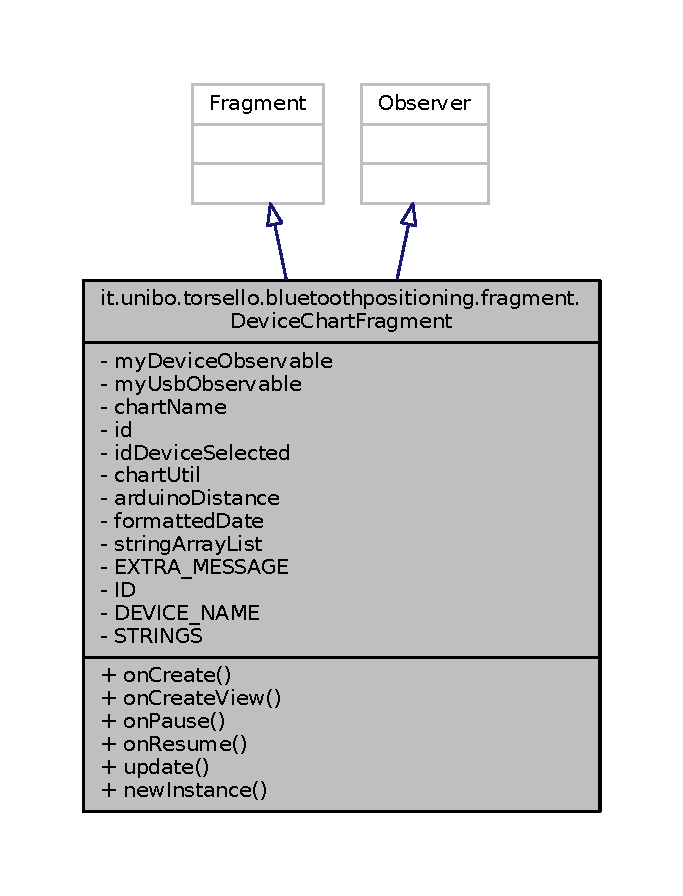
\includegraphics[width=328pt]{classit_1_1unibo_1_1torsello_1_1bluetoothpositioning_1_1fragment_1_1DeviceChartFragment__inherit__graph}
\end{center}
\end{figure}


Diagramma di collaborazione per it.\+unibo.\+torsello.\+bluetoothpositioning.\+fragment.\+Device\+Chart\+Fragment\+:
\nopagebreak
\begin{figure}[H]
\begin{center}
\leavevmode
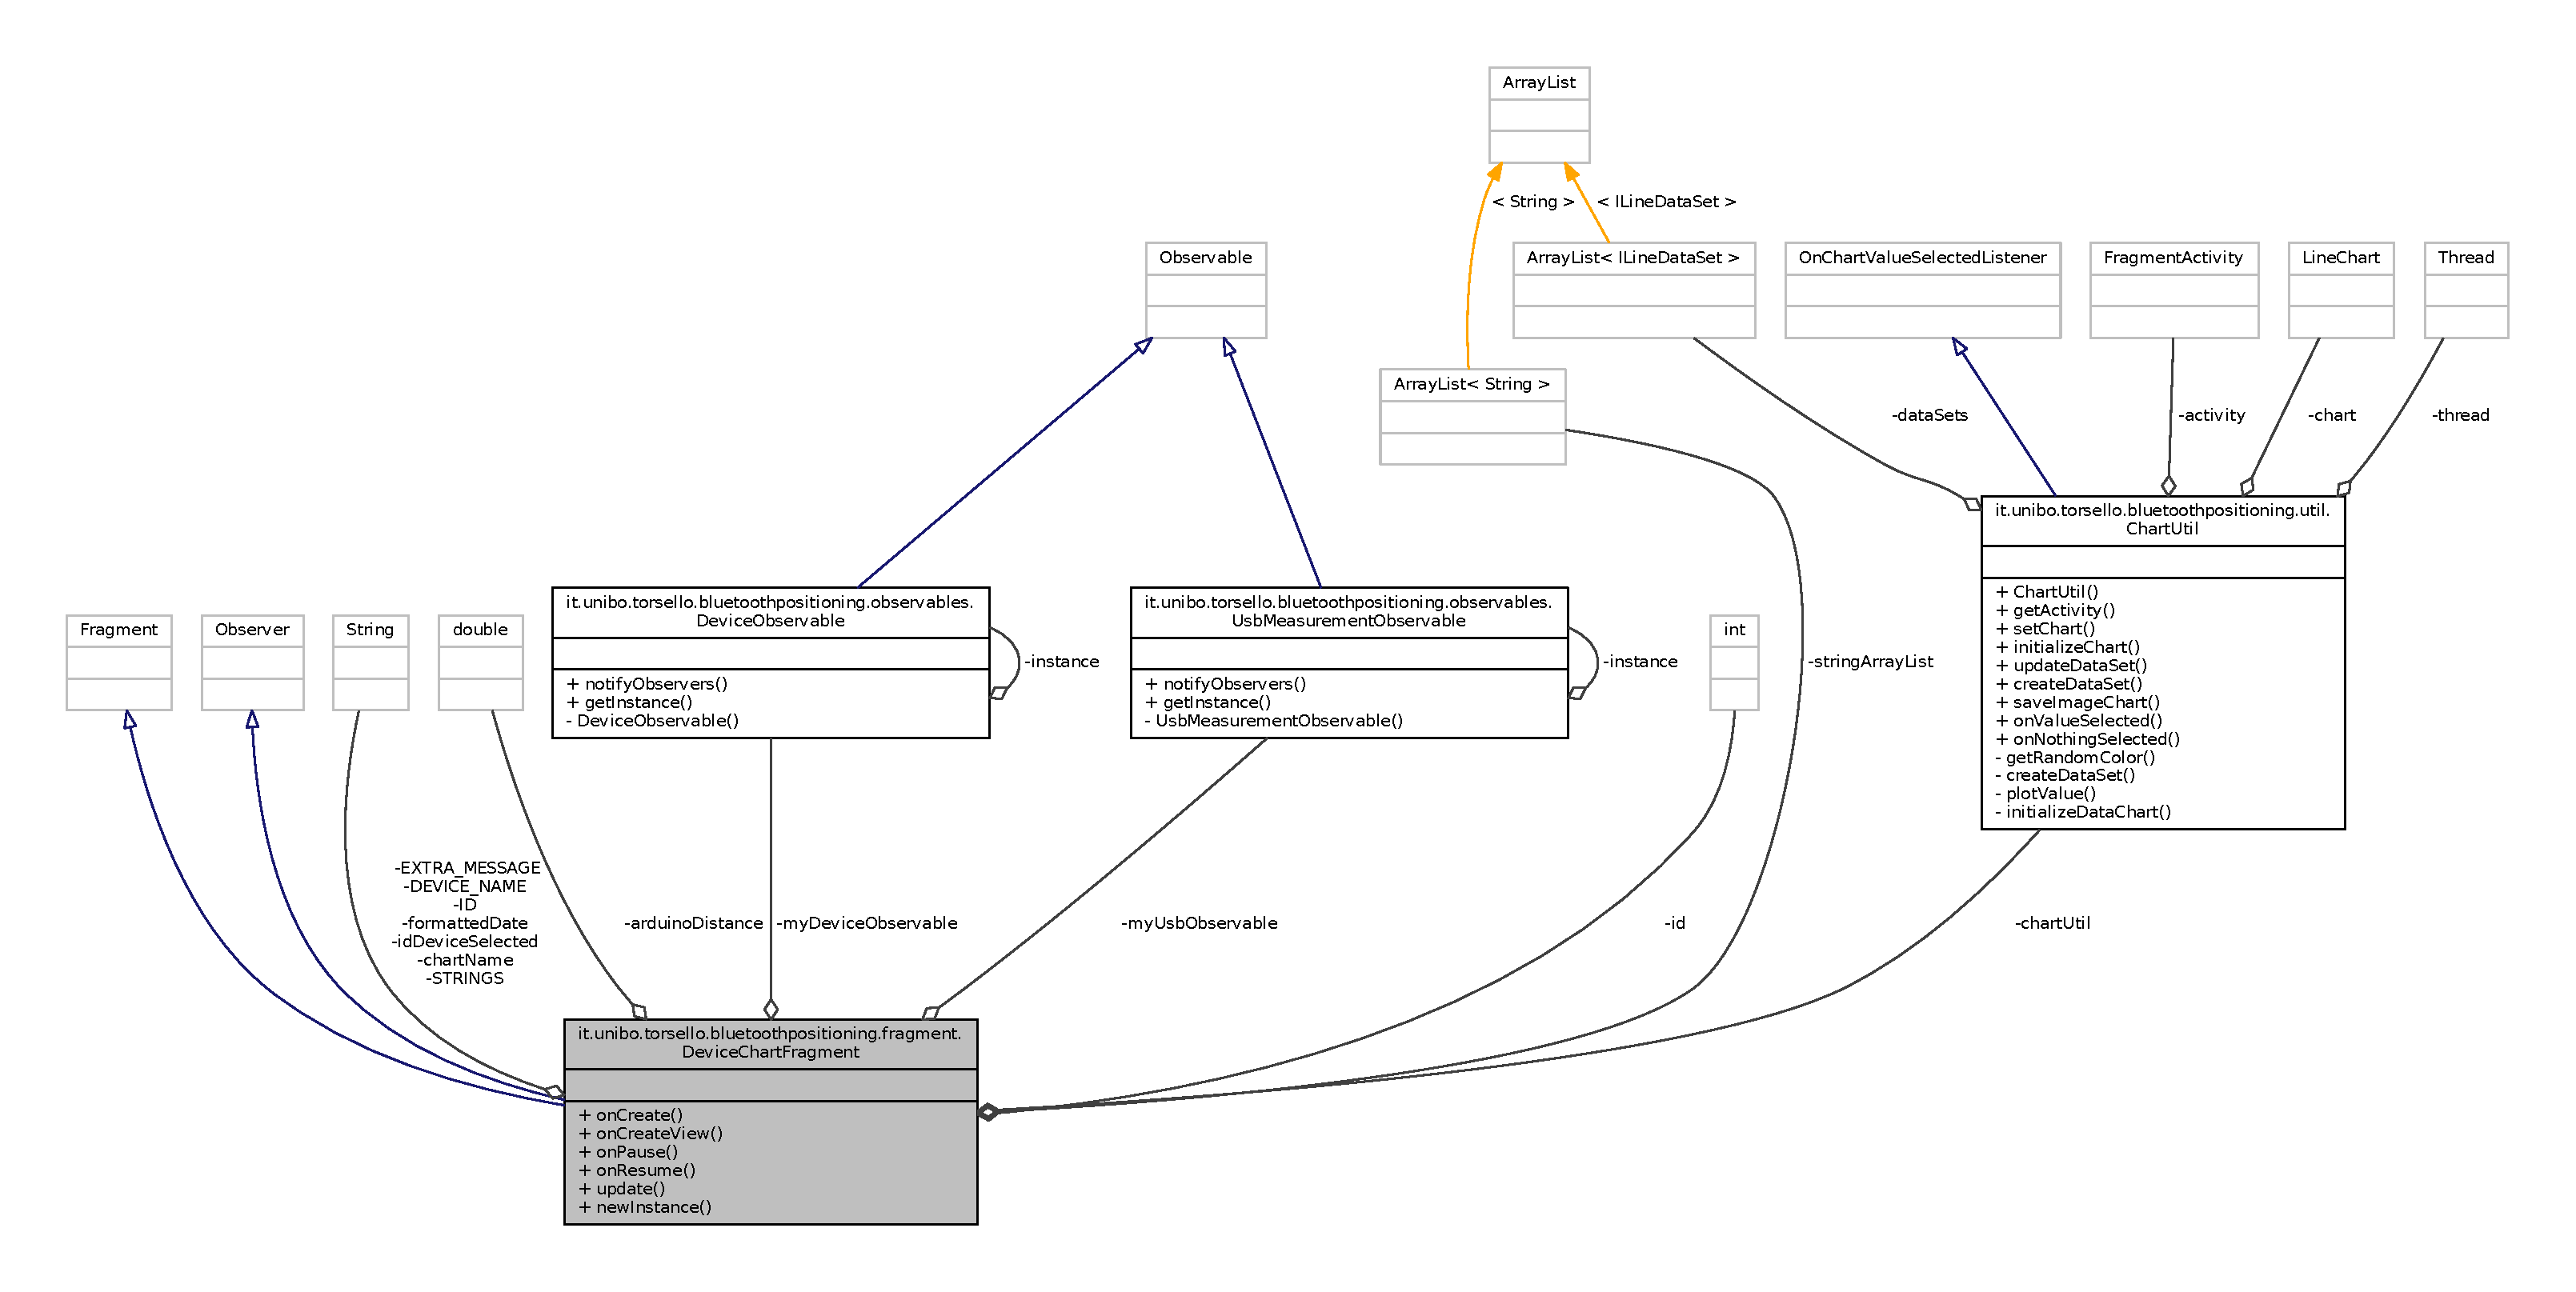
\includegraphics[width=350pt]{classit_1_1unibo_1_1torsello_1_1bluetoothpositioning_1_1fragment_1_1DeviceChartFragment__coll__graph}
\end{center}
\end{figure}
\subsubsection*{Membri pubblici}
\begin{DoxyCompactItemize}
\item 
void \hyperlink{classit_1_1unibo_1_1torsello_1_1bluetoothpositioning_1_1fragment_1_1DeviceChartFragment_a08829e4742056e3f4ba3561c3de1e3d6_a08829e4742056e3f4ba3561c3de1e3d6}{on\+Create} (Bundle saved\+Instance\+State)
\item 
View \hyperlink{classit_1_1unibo_1_1torsello_1_1bluetoothpositioning_1_1fragment_1_1DeviceChartFragment_ae4d8a0e874dc5cd856de7424bc9269f0_ae4d8a0e874dc5cd856de7424bc9269f0}{on\+Create\+View} (Layout\+Inflater inflater, View\+Group container, Bundle saved\+Instance\+State)
\item 
void \hyperlink{classit_1_1unibo_1_1torsello_1_1bluetoothpositioning_1_1fragment_1_1DeviceChartFragment_a55f65f257b5facf73fb3ec7df689cbbb_a55f65f257b5facf73fb3ec7df689cbbb}{on\+Pause} ()
\item 
void \hyperlink{classit_1_1unibo_1_1torsello_1_1bluetoothpositioning_1_1fragment_1_1DeviceChartFragment_a039e605be958cf11403bc1358bfd70c0_a039e605be958cf11403bc1358bfd70c0}{on\+Resume} ()
\item 
void \hyperlink{classit_1_1unibo_1_1torsello_1_1bluetoothpositioning_1_1fragment_1_1DeviceChartFragment_a879725f924473013057be7f3aaea2ab0_a879725f924473013057be7f3aaea2ab0}{update} (Observable observable, Object arg)
\end{DoxyCompactItemize}
\subsubsection*{Membri pubblici statici}
\begin{DoxyCompactItemize}
\item 
static \hyperlink{classit_1_1unibo_1_1torsello_1_1bluetoothpositioning_1_1fragment_1_1DeviceChartFragment}{Device\+Chart\+Fragment} \hyperlink{classit_1_1unibo_1_1torsello_1_1bluetoothpositioning_1_1fragment_1_1DeviceChartFragment_a16fb051f584eb5fd324e25ce67cc6730_a16fb051f584eb5fd324e25ce67cc6730}{new\+Instance} (String message, int \hyperlink{classit_1_1unibo_1_1torsello_1_1bluetoothpositioning_1_1fragment_1_1DeviceChartFragment_a93b0dbe70e24a27e96f52c5135006564_a93b0dbe70e24a27e96f52c5135006564}{id}, String device\+Name, Array\+List$<$ String $>$ strings)
\end{DoxyCompactItemize}
\subsubsection*{Attributi privati}
\begin{DoxyCompactItemize}
\item 
\hyperlink{classit_1_1unibo_1_1torsello_1_1bluetoothpositioning_1_1observables_1_1DeviceObservable}{Device\+Observable} \hyperlink{classit_1_1unibo_1_1torsello_1_1bluetoothpositioning_1_1fragment_1_1DeviceChartFragment_a82756c59ac344db249e6cebcec3d1835_a82756c59ac344db249e6cebcec3d1835}{my\+Device\+Observable}
\item 
\hyperlink{classit_1_1unibo_1_1torsello_1_1bluetoothpositioning_1_1observables_1_1UsbMeasurementObservable}{Usb\+Measurement\+Observable} \hyperlink{classit_1_1unibo_1_1torsello_1_1bluetoothpositioning_1_1fragment_1_1DeviceChartFragment_aa9e0527dce7ccc3e51afe698a76f2faf_aa9e0527dce7ccc3e51afe698a76f2faf}{my\+Usb\+Observable}
\item 
String \hyperlink{classit_1_1unibo_1_1torsello_1_1bluetoothpositioning_1_1fragment_1_1DeviceChartFragment_a3ad9d4a2c35dc877d54b82168620c449_a3ad9d4a2c35dc877d54b82168620c449}{chart\+Name}
\item 
int \hyperlink{classit_1_1unibo_1_1torsello_1_1bluetoothpositioning_1_1fragment_1_1DeviceChartFragment_a93b0dbe70e24a27e96f52c5135006564_a93b0dbe70e24a27e96f52c5135006564}{id}
\item 
String \hyperlink{classit_1_1unibo_1_1torsello_1_1bluetoothpositioning_1_1fragment_1_1DeviceChartFragment_a5140a40f33827bd14ea68efe8157ee06_a5140a40f33827bd14ea68efe8157ee06}{id\+Device\+Selected}
\item 
\hyperlink{classit_1_1unibo_1_1torsello_1_1bluetoothpositioning_1_1util_1_1ChartUtil}{Chart\+Util} \hyperlink{classit_1_1unibo_1_1torsello_1_1bluetoothpositioning_1_1fragment_1_1DeviceChartFragment_ad28ad16d89e075ea2e572bba9b24bc4e_ad28ad16d89e075ea2e572bba9b24bc4e}{chart\+Util}
\item 
double \hyperlink{classit_1_1unibo_1_1torsello_1_1bluetoothpositioning_1_1fragment_1_1DeviceChartFragment_ac62d852fec179fcadd6caa94d4087d67_ac62d852fec179fcadd6caa94d4087d67}{arduino\+Distance} = 0D
\item 
String \hyperlink{classit_1_1unibo_1_1torsello_1_1bluetoothpositioning_1_1fragment_1_1DeviceChartFragment_a9a927b3e1271a11093f62a53d294f908_a9a927b3e1271a11093f62a53d294f908}{formatted\+Date}
\item 
Array\+List$<$ String $>$ \hyperlink{classit_1_1unibo_1_1torsello_1_1bluetoothpositioning_1_1fragment_1_1DeviceChartFragment_a52b2534176114632fe412b609fef559e_a52b2534176114632fe412b609fef559e}{string\+Array\+List}
\end{DoxyCompactItemize}
\subsubsection*{Attributi privati statici}
\begin{DoxyCompactItemize}
\item 
static final String \hyperlink{classit_1_1unibo_1_1torsello_1_1bluetoothpositioning_1_1fragment_1_1DeviceChartFragment_a28ddce9b6c06c183ca8a3717e51d6339_a28ddce9b6c06c183ca8a3717e51d6339}{E\+X\+T\+R\+A\+\_\+\+M\+E\+S\+S\+A\+GE} = \char`\"{}E\+X\+T\+R\+A\+\_\+\+M\+E\+S\+S\+A\+GE\char`\"{}
\item 
static final String \hyperlink{classit_1_1unibo_1_1torsello_1_1bluetoothpositioning_1_1fragment_1_1DeviceChartFragment_a4f077af11a4bef4240a1fe8e2185c20e_a4f077af11a4bef4240a1fe8e2185c20e}{ID} = \char`\"{}ID\char`\"{}
\item 
static final String \hyperlink{classit_1_1unibo_1_1torsello_1_1bluetoothpositioning_1_1fragment_1_1DeviceChartFragment_a9313a4d6f386037e62d95d535b379ab2_a9313a4d6f386037e62d95d535b379ab2}{D\+E\+V\+I\+C\+E\+\_\+\+N\+A\+ME} = \char`\"{}D\+E\+V\+I\+C\+E\+\_\+\+N\+A\+ME\char`\"{}
\item 
static final String \hyperlink{classit_1_1unibo_1_1torsello_1_1bluetoothpositioning_1_1fragment_1_1DeviceChartFragment_a2be86b68a5ce90a3ba90b7a214ac47c0_a2be86b68a5ce90a3ba90b7a214ac47c0}{S\+T\+R\+I\+N\+GS} = \char`\"{}S\+T\+R\+I\+N\+GS\char`\"{}
\end{DoxyCompactItemize}


\subsubsection{Descrizione dettagliata}
Created by Federico Torsello. \href{mailto:federico.torsello@studio.unibo.it}{\tt federico.\+torsello@studio.\+unibo.\+it} 

\subsubsection{Documentazione delle funzioni membro}
\hypertarget{classit_1_1unibo_1_1torsello_1_1bluetoothpositioning_1_1fragment_1_1DeviceChartFragment_a16fb051f584eb5fd324e25ce67cc6730_a16fb051f584eb5fd324e25ce67cc6730}{}\label{classit_1_1unibo_1_1torsello_1_1bluetoothpositioning_1_1fragment_1_1DeviceChartFragment_a16fb051f584eb5fd324e25ce67cc6730_a16fb051f584eb5fd324e25ce67cc6730} 
\index{it\+::unibo\+::torsello\+::bluetoothpositioning\+::fragment\+::\+Device\+Chart\+Fragment@{it\+::unibo\+::torsello\+::bluetoothpositioning\+::fragment\+::\+Device\+Chart\+Fragment}!new\+Instance@{new\+Instance}}
\index{new\+Instance@{new\+Instance}!it\+::unibo\+::torsello\+::bluetoothpositioning\+::fragment\+::\+Device\+Chart\+Fragment@{it\+::unibo\+::torsello\+::bluetoothpositioning\+::fragment\+::\+Device\+Chart\+Fragment}}
\paragraph{\texorpdfstring{new\+Instance()}{newInstance()}}
{\footnotesize\ttfamily static \hyperlink{classit_1_1unibo_1_1torsello_1_1bluetoothpositioning_1_1fragment_1_1DeviceChartFragment}{Device\+Chart\+Fragment} it.\+unibo.\+torsello.\+bluetoothpositioning.\+fragment.\+Device\+Chart\+Fragment.\+new\+Instance (\begin{DoxyParamCaption}\item[{String}]{message,  }\item[{int}]{id,  }\item[{String}]{device\+Name,  }\item[{Array\+List$<$ String $>$}]{strings }\end{DoxyParamCaption})\hspace{0.3cm}{\ttfamily [static]}}


\begin{DoxyCode}
52                                                                              \{
53         DeviceChartFragment fragment = \textcolor{keyword}{new} DeviceChartFragment();
54         Bundle args = \textcolor{keyword}{new} Bundle();
55         args.putString(\hyperlink{classit_1_1unibo_1_1torsello_1_1bluetoothpositioning_1_1fragment_1_1DeviceChartFragment_a28ddce9b6c06c183ca8a3717e51d6339_a28ddce9b6c06c183ca8a3717e51d6339}{EXTRA\_MESSAGE}, message);
56         args.putInt(\hyperlink{classit_1_1unibo_1_1torsello_1_1bluetoothpositioning_1_1fragment_1_1DeviceChartFragment_a4f077af11a4bef4240a1fe8e2185c20e_a4f077af11a4bef4240a1fe8e2185c20e}{ID}, \textcolor{keywordtype}{id});
57         args.putString(\hyperlink{classit_1_1unibo_1_1torsello_1_1bluetoothpositioning_1_1fragment_1_1DeviceChartFragment_a9313a4d6f386037e62d95d535b379ab2_a9313a4d6f386037e62d95d535b379ab2}{DEVICE\_NAME}, deviceName);
58         args.putStringArrayList(\hyperlink{classit_1_1unibo_1_1torsello_1_1bluetoothpositioning_1_1fragment_1_1DeviceChartFragment_a2be86b68a5ce90a3ba90b7a214ac47c0_a2be86b68a5ce90a3ba90b7a214ac47c0}{STRINGS}, strings);
59         fragment.setArguments(args);
60         \textcolor{keywordflow}{return} fragment;
61     \}
\end{DoxyCode}
\hypertarget{classit_1_1unibo_1_1torsello_1_1bluetoothpositioning_1_1fragment_1_1DeviceChartFragment_a08829e4742056e3f4ba3561c3de1e3d6_a08829e4742056e3f4ba3561c3de1e3d6}{}\label{classit_1_1unibo_1_1torsello_1_1bluetoothpositioning_1_1fragment_1_1DeviceChartFragment_a08829e4742056e3f4ba3561c3de1e3d6_a08829e4742056e3f4ba3561c3de1e3d6} 
\index{it\+::unibo\+::torsello\+::bluetoothpositioning\+::fragment\+::\+Device\+Chart\+Fragment@{it\+::unibo\+::torsello\+::bluetoothpositioning\+::fragment\+::\+Device\+Chart\+Fragment}!on\+Create@{on\+Create}}
\index{on\+Create@{on\+Create}!it\+::unibo\+::torsello\+::bluetoothpositioning\+::fragment\+::\+Device\+Chart\+Fragment@{it\+::unibo\+::torsello\+::bluetoothpositioning\+::fragment\+::\+Device\+Chart\+Fragment}}
\paragraph{\texorpdfstring{on\+Create()}{onCreate()}}
{\footnotesize\ttfamily void it.\+unibo.\+torsello.\+bluetoothpositioning.\+fragment.\+Device\+Chart\+Fragment.\+on\+Create (\begin{DoxyParamCaption}\item[{Bundle}]{saved\+Instance\+State }\end{DoxyParamCaption})}


\begin{DoxyCode}
64                                                     \{
65         super.onCreate(savedInstanceState);
66 
67         \textcolor{keywordtype}{id} = getArguments().getInt(\hyperlink{classit_1_1unibo_1_1torsello_1_1bluetoothpositioning_1_1fragment_1_1DeviceChartFragment_a4f077af11a4bef4240a1fe8e2185c20e_a4f077af11a4bef4240a1fe8e2185c20e}{ID});
68         \hyperlink{classit_1_1unibo_1_1torsello_1_1bluetoothpositioning_1_1fragment_1_1DeviceChartFragment_a3ad9d4a2c35dc877d54b82168620c449_a3ad9d4a2c35dc877d54b82168620c449}{chartName} = getArguments().getString(\hyperlink{classit_1_1unibo_1_1torsello_1_1bluetoothpositioning_1_1fragment_1_1DeviceChartFragment_a28ddce9b6c06c183ca8a3717e51d6339_a28ddce9b6c06c183ca8a3717e51d6339}{EXTRA\_MESSAGE});
69         \hyperlink{classit_1_1unibo_1_1torsello_1_1bluetoothpositioning_1_1fragment_1_1DeviceChartFragment_a5140a40f33827bd14ea68efe8157ee06_a5140a40f33827bd14ea68efe8157ee06}{idDeviceSelected} = getArguments().getString(\hyperlink{classit_1_1unibo_1_1torsello_1_1bluetoothpositioning_1_1fragment_1_1DeviceChartFragment_a9313a4d6f386037e62d95d535b379ab2_a9313a4d6f386037e62d95d535b379ab2}{DEVICE\_NAME});
70         \hyperlink{classit_1_1unibo_1_1torsello_1_1bluetoothpositioning_1_1fragment_1_1DeviceChartFragment_a52b2534176114632fe412b609fef559e_a52b2534176114632fe412b609fef559e}{stringArrayList} = getArguments().getStringArrayList(
      \hyperlink{classit_1_1unibo_1_1torsello_1_1bluetoothpositioning_1_1fragment_1_1DeviceChartFragment_a2be86b68a5ce90a3ba90b7a214ac47c0_a2be86b68a5ce90a3ba90b7a214ac47c0}{STRINGS});
71 
72         \hyperlink{classit_1_1unibo_1_1torsello_1_1bluetoothpositioning_1_1fragment_1_1DeviceChartFragment_a82756c59ac344db249e6cebcec3d1835_a82756c59ac344db249e6cebcec3d1835}{myDeviceObservable} = DeviceObservable.\hyperlink{classit_1_1unibo_1_1torsello_1_1bluetoothpositioning_1_1observables_1_1DeviceObservable_ab16792c5848440646624b2a41553954a_ab16792c5848440646624b2a41553954a}{getInstance}();
73         \hyperlink{classit_1_1unibo_1_1torsello_1_1bluetoothpositioning_1_1fragment_1_1DeviceChartFragment_aa9e0527dce7ccc3e51afe698a76f2faf_aa9e0527dce7ccc3e51afe698a76f2faf}{myUsbObservable} = UsbMeasurementObservable.\hyperlink{classit_1_1unibo_1_1torsello_1_1bluetoothpositioning_1_1observables_1_1UsbMeasurementObservable_aff4f89490f3f2c11ca4feea933d12d88_aff4f89490f3f2c11ca4feea933d12d88}{getInstance}();
74 
75         \hyperlink{classit_1_1unibo_1_1torsello_1_1bluetoothpositioning_1_1fragment_1_1DeviceChartFragment_ad28ad16d89e075ea2e572bba9b24bc4e_ad28ad16d89e075ea2e572bba9b24bc4e}{chartUtil} = \textcolor{keyword}{new} ChartUtil(getActivity());
76 
77         SimpleDateFormat df = \textcolor{keyword}{new} SimpleDateFormat(\textcolor{stringliteral}{"dd-MMM-yyyy"}, Locale.getDefault());
78         \hyperlink{classit_1_1unibo_1_1torsello_1_1bluetoothpositioning_1_1fragment_1_1DeviceChartFragment_a9a927b3e1271a11093f62a53d294f908_a9a927b3e1271a11093f62a53d294f908}{formattedDate} = df.format(Calendar.getInstance().getTime());
79     \}
\end{DoxyCode}
\hypertarget{classit_1_1unibo_1_1torsello_1_1bluetoothpositioning_1_1fragment_1_1DeviceChartFragment_ae4d8a0e874dc5cd856de7424bc9269f0_ae4d8a0e874dc5cd856de7424bc9269f0}{}\label{classit_1_1unibo_1_1torsello_1_1bluetoothpositioning_1_1fragment_1_1DeviceChartFragment_ae4d8a0e874dc5cd856de7424bc9269f0_ae4d8a0e874dc5cd856de7424bc9269f0} 
\index{it\+::unibo\+::torsello\+::bluetoothpositioning\+::fragment\+::\+Device\+Chart\+Fragment@{it\+::unibo\+::torsello\+::bluetoothpositioning\+::fragment\+::\+Device\+Chart\+Fragment}!on\+Create\+View@{on\+Create\+View}}
\index{on\+Create\+View@{on\+Create\+View}!it\+::unibo\+::torsello\+::bluetoothpositioning\+::fragment\+::\+Device\+Chart\+Fragment@{it\+::unibo\+::torsello\+::bluetoothpositioning\+::fragment\+::\+Device\+Chart\+Fragment}}
\paragraph{\texorpdfstring{on\+Create\+View()}{onCreateView()}}
{\footnotesize\ttfamily View it.\+unibo.\+torsello.\+bluetoothpositioning.\+fragment.\+Device\+Chart\+Fragment.\+on\+Create\+View (\begin{DoxyParamCaption}\item[{Layout\+Inflater}]{inflater,  }\item[{View\+Group}]{container,  }\item[{Bundle}]{saved\+Instance\+State }\end{DoxyParamCaption})}


\begin{DoxyCode}
82                                                                                                       \{
83 
84         View root = inflater.inflate(R.layout.fragment\_device\_detail\_chart, container, \textcolor{keyword}{false});
85 
86         Button button = (Button) root.findViewById(R.id.button\_save\_image);
87         button.setOnClickListener(\textcolor{keyword}{new} View.OnClickListener() \{
88             @Override
89             \textcolor{keyword}{public} \textcolor{keywordtype}{void} onClick(View v) \{
90                 \hyperlink{classit_1_1unibo_1_1torsello_1_1bluetoothpositioning_1_1fragment_1_1DeviceChartFragment_ad28ad16d89e075ea2e572bba9b24bc4e_ad28ad16d89e075ea2e572bba9b24bc4e}{chartUtil}.\hyperlink{classit_1_1unibo_1_1torsello_1_1bluetoothpositioning_1_1util_1_1ChartUtil_afdbdcf15b073da5b03613dbccc7681a9_afdbdcf15b073da5b03613dbccc7681a9}{saveImageChart}(\hyperlink{classit_1_1unibo_1_1torsello_1_1bluetoothpositioning_1_1fragment_1_1DeviceChartFragment_a3ad9d4a2c35dc877d54b82168620c449_a3ad9d4a2c35dc877d54b82168620c449}{chartName}, 
      \hyperlink{classit_1_1unibo_1_1torsello_1_1bluetoothpositioning_1_1fragment_1_1DeviceChartFragment_a9a927b3e1271a11093f62a53d294f908_a9a927b3e1271a11093f62a53d294f908}{formattedDate});
91             \}
92         \});
93 
94         LineChart lineChart = (LineChart) root.findViewById(R.id.chart);
95 
96         \textcolor{comment}{// add the charts}
97         \hyperlink{classit_1_1unibo_1_1torsello_1_1bluetoothpositioning_1_1fragment_1_1DeviceChartFragment_ad28ad16d89e075ea2e572bba9b24bc4e_ad28ad16d89e075ea2e572bba9b24bc4e}{chartUtil}.\hyperlink{classit_1_1unibo_1_1torsello_1_1bluetoothpositioning_1_1util_1_1ChartUtil_a26e84414723ff1ca38d8f2907ed3322e_a26e84414723ff1ca38d8f2907ed3322e}{setChart}(lineChart);
98 
99         \textcolor{keywordflow}{return} root;
100     \}
\end{DoxyCode}
\hypertarget{classit_1_1unibo_1_1torsello_1_1bluetoothpositioning_1_1fragment_1_1DeviceChartFragment_a55f65f257b5facf73fb3ec7df689cbbb_a55f65f257b5facf73fb3ec7df689cbbb}{}\label{classit_1_1unibo_1_1torsello_1_1bluetoothpositioning_1_1fragment_1_1DeviceChartFragment_a55f65f257b5facf73fb3ec7df689cbbb_a55f65f257b5facf73fb3ec7df689cbbb} 
\index{it\+::unibo\+::torsello\+::bluetoothpositioning\+::fragment\+::\+Device\+Chart\+Fragment@{it\+::unibo\+::torsello\+::bluetoothpositioning\+::fragment\+::\+Device\+Chart\+Fragment}!on\+Pause@{on\+Pause}}
\index{on\+Pause@{on\+Pause}!it\+::unibo\+::torsello\+::bluetoothpositioning\+::fragment\+::\+Device\+Chart\+Fragment@{it\+::unibo\+::torsello\+::bluetoothpositioning\+::fragment\+::\+Device\+Chart\+Fragment}}
\paragraph{\texorpdfstring{on\+Pause()}{onPause()}}
{\footnotesize\ttfamily void it.\+unibo.\+torsello.\+bluetoothpositioning.\+fragment.\+Device\+Chart\+Fragment.\+on\+Pause (\begin{DoxyParamCaption}{ }\end{DoxyParamCaption})}


\begin{DoxyCode}
103                           \{
104         \hyperlink{classit_1_1unibo_1_1torsello_1_1bluetoothpositioning_1_1fragment_1_1DeviceChartFragment_a82756c59ac344db249e6cebcec3d1835_a82756c59ac344db249e6cebcec3d1835}{myDeviceObservable}.deleteObserver(\textcolor{keyword}{this});
105         \hyperlink{classit_1_1unibo_1_1torsello_1_1bluetoothpositioning_1_1fragment_1_1DeviceChartFragment_aa9e0527dce7ccc3e51afe698a76f2faf_aa9e0527dce7ccc3e51afe698a76f2faf}{myUsbObservable}.deleteObserver(\textcolor{keyword}{this});
106         super.onPause();
107     \}
\end{DoxyCode}
\hypertarget{classit_1_1unibo_1_1torsello_1_1bluetoothpositioning_1_1fragment_1_1DeviceChartFragment_a039e605be958cf11403bc1358bfd70c0_a039e605be958cf11403bc1358bfd70c0}{}\label{classit_1_1unibo_1_1torsello_1_1bluetoothpositioning_1_1fragment_1_1DeviceChartFragment_a039e605be958cf11403bc1358bfd70c0_a039e605be958cf11403bc1358bfd70c0} 
\index{it\+::unibo\+::torsello\+::bluetoothpositioning\+::fragment\+::\+Device\+Chart\+Fragment@{it\+::unibo\+::torsello\+::bluetoothpositioning\+::fragment\+::\+Device\+Chart\+Fragment}!on\+Resume@{on\+Resume}}
\index{on\+Resume@{on\+Resume}!it\+::unibo\+::torsello\+::bluetoothpositioning\+::fragment\+::\+Device\+Chart\+Fragment@{it\+::unibo\+::torsello\+::bluetoothpositioning\+::fragment\+::\+Device\+Chart\+Fragment}}
\paragraph{\texorpdfstring{on\+Resume()}{onResume()}}
{\footnotesize\ttfamily void it.\+unibo.\+torsello.\+bluetoothpositioning.\+fragment.\+Device\+Chart\+Fragment.\+on\+Resume (\begin{DoxyParamCaption}{ }\end{DoxyParamCaption})}


\begin{DoxyCode}
110                            \{
111         super.onResume();
112         \hyperlink{classit_1_1unibo_1_1torsello_1_1bluetoothpositioning_1_1fragment_1_1DeviceChartFragment_a82756c59ac344db249e6cebcec3d1835_a82756c59ac344db249e6cebcec3d1835}{myDeviceObservable}.addObserver(\textcolor{keyword}{this});
113         \hyperlink{classit_1_1unibo_1_1torsello_1_1bluetoothpositioning_1_1fragment_1_1DeviceChartFragment_aa9e0527dce7ccc3e51afe698a76f2faf_aa9e0527dce7ccc3e51afe698a76f2faf}{myUsbObservable}.addObserver(\textcolor{keyword}{this});
114         \hyperlink{classit_1_1unibo_1_1torsello_1_1bluetoothpositioning_1_1fragment_1_1DeviceChartFragment_ad28ad16d89e075ea2e572bba9b24bc4e_ad28ad16d89e075ea2e572bba9b24bc4e}{chartUtil}.\hyperlink{classit_1_1unibo_1_1torsello_1_1bluetoothpositioning_1_1util_1_1ChartUtil_aab1a6bd41cbf8228c53d633af6b89bb7_aab1a6bd41cbf8228c53d633af6b89bb7}{initializeChart}();
115     \}
\end{DoxyCode}
\hypertarget{classit_1_1unibo_1_1torsello_1_1bluetoothpositioning_1_1fragment_1_1DeviceChartFragment_a879725f924473013057be7f3aaea2ab0_a879725f924473013057be7f3aaea2ab0}{}\label{classit_1_1unibo_1_1torsello_1_1bluetoothpositioning_1_1fragment_1_1DeviceChartFragment_a879725f924473013057be7f3aaea2ab0_a879725f924473013057be7f3aaea2ab0} 
\index{it\+::unibo\+::torsello\+::bluetoothpositioning\+::fragment\+::\+Device\+Chart\+Fragment@{it\+::unibo\+::torsello\+::bluetoothpositioning\+::fragment\+::\+Device\+Chart\+Fragment}!update@{update}}
\index{update@{update}!it\+::unibo\+::torsello\+::bluetoothpositioning\+::fragment\+::\+Device\+Chart\+Fragment@{it\+::unibo\+::torsello\+::bluetoothpositioning\+::fragment\+::\+Device\+Chart\+Fragment}}
\paragraph{\texorpdfstring{update()}{update()}}
{\footnotesize\ttfamily void it.\+unibo.\+torsello.\+bluetoothpositioning.\+fragment.\+Device\+Chart\+Fragment.\+update (\begin{DoxyParamCaption}\item[{Observable}]{observable,  }\item[{Object}]{arg }\end{DoxyParamCaption})}


\begin{DoxyCode}
118                                                           \{
119 
120         \textcolor{keywordflow}{if} (observable instanceof UsbMeasurementObservable) \{
121             \textcolor{keywordflow}{if} (arg instanceof Double) \{
122                 \hyperlink{classit_1_1unibo_1_1torsello_1_1bluetoothpositioning_1_1fragment_1_1DeviceChartFragment_ac62d852fec179fcadd6caa94d4087d67_ac62d852fec179fcadd6caa94d4087d67}{arduinoDistance} = (Double) arg;
123             \}
124         \}
125 
126         \textcolor{keywordflow}{if} (observable instanceof DeviceObservable) \{
127             \textcolor{keywordflow}{if} (arg instanceof List) \{
128 
129                 List<Device> devices = (List<Device>) arg;
130 
131                 \textcolor{keywordflow}{for} (Device deviceSelected : devices) \{
132                     \textcolor{keywordflow}{if} (deviceSelected.getFriendlyName().equals(\hyperlink{classit_1_1unibo_1_1torsello_1_1bluetoothpositioning_1_1fragment_1_1DeviceChartFragment_a5140a40f33827bd14ea68efe8157ee06_a5140a40f33827bd14ea68efe8157ee06}{idDeviceSelected}) ||
133                             deviceSelected.getAddress().equals(\hyperlink{classit_1_1unibo_1_1torsello_1_1bluetoothpositioning_1_1fragment_1_1DeviceChartFragment_a5140a40f33827bd14ea68efe8157ee06_a5140a40f33827bd14ea68efe8157ee06}{idDeviceSelected})) \{
134 
135                         \textcolor{keywordflow}{if} (\hyperlink{classit_1_1unibo_1_1torsello_1_1bluetoothpositioning_1_1fragment_1_1DeviceChartFragment_ad28ad16d89e075ea2e572bba9b24bc4e_ad28ad16d89e075ea2e572bba9b24bc4e}{chartUtil} != null) \{
136 
137                             \hyperlink{classit_1_1unibo_1_1torsello_1_1bluetoothpositioning_1_1fragment_1_1DeviceChartFragment_ad28ad16d89e075ea2e572bba9b24bc4e_ad28ad16d89e075ea2e572bba9b24bc4e}{chartUtil}.\hyperlink{classit_1_1unibo_1_1torsello_1_1bluetoothpositioning_1_1util_1_1ChartUtil_a7460cb57f8ad402dc522b592bc40f7b2_a7460cb57f8ad402dc522b592bc40f7b2}{createDataSet}(
      \hyperlink{classit_1_1unibo_1_1torsello_1_1bluetoothpositioning_1_1fragment_1_1DeviceChartFragment_a52b2534176114632fe412b609fef559e_a52b2534176114632fe412b609fef559e}{stringArrayList});
138 
139                             ArrayList<Double> dataSetForUpdates = \textcolor{keyword}{new} ArrayList<>();
140 
141                             \textcolor{keywordflow}{for} (String s : \hyperlink{classit_1_1unibo_1_1torsello_1_1bluetoothpositioning_1_1fragment_1_1DeviceChartFragment_a52b2534176114632fe412b609fef559e_a52b2534176114632fe412b609fef559e}{stringArrayList}) \{
142                                 \textcolor{keywordflow}{if} (s.equals(getString(R.string.chart\_arduino))) \{
143                                     dataSetForUpdates.add(\hyperlink{classit_1_1unibo_1_1torsello_1_1bluetoothpositioning_1_1fragment_1_1DeviceChartFragment_ac62d852fec179fcadd6caa94d4087d67_ac62d852fec179fcadd6caa94d4087d67}{arduinoDistance});
144                                 \}
145 
146                                 \textcolor{keywordflow}{if} (s.equals(getString(R.string.chart\_raw\_distance))) \{
147                                     dataSetForUpdates.add(deviceSelected.getRawDistance());
148                                 \}
149 
150                                 \textcolor{keywordflow}{if} (s.equals(getString(R.string.chart\_altbeacon))) \{
151                                     dataSetForUpdates.add(deviceSelected.getAltBeaconDistance());
152 
153                                 \}
154 
155                                 \textcolor{keywordflow}{if} (s.equals(getString(R.string.chart\_kalman\_filter))) \{
156                                     dataSetForUpdates.add(deviceSelected.getKalmanFilterDistance());
157                                 \}
158                             \}
159 
160                             \hyperlink{classit_1_1unibo_1_1torsello_1_1bluetoothpositioning_1_1fragment_1_1DeviceChartFragment_ad28ad16d89e075ea2e572bba9b24bc4e_ad28ad16d89e075ea2e572bba9b24bc4e}{chartUtil}.\hyperlink{classit_1_1unibo_1_1torsello_1_1bluetoothpositioning_1_1util_1_1ChartUtil_aa9bda04d2c2058fb1b3fcd72c5a7471d_aa9bda04d2c2058fb1b3fcd72c5a7471d}{updateDataSet}(dataSetForUpdates);
161                         \}
162                     \}
163                 \}
164             \}
165         \}
166     \}
\end{DoxyCode}


\subsubsection{Documentazione dei membri dato}
\hypertarget{classit_1_1unibo_1_1torsello_1_1bluetoothpositioning_1_1fragment_1_1DeviceChartFragment_ac62d852fec179fcadd6caa94d4087d67_ac62d852fec179fcadd6caa94d4087d67}{}\label{classit_1_1unibo_1_1torsello_1_1bluetoothpositioning_1_1fragment_1_1DeviceChartFragment_ac62d852fec179fcadd6caa94d4087d67_ac62d852fec179fcadd6caa94d4087d67} 
\index{it\+::unibo\+::torsello\+::bluetoothpositioning\+::fragment\+::\+Device\+Chart\+Fragment@{it\+::unibo\+::torsello\+::bluetoothpositioning\+::fragment\+::\+Device\+Chart\+Fragment}!arduino\+Distance@{arduino\+Distance}}
\index{arduino\+Distance@{arduino\+Distance}!it\+::unibo\+::torsello\+::bluetoothpositioning\+::fragment\+::\+Device\+Chart\+Fragment@{it\+::unibo\+::torsello\+::bluetoothpositioning\+::fragment\+::\+Device\+Chart\+Fragment}}
\paragraph{\texorpdfstring{arduino\+Distance}{arduinoDistance}}
{\footnotesize\ttfamily double it.\+unibo.\+torsello.\+bluetoothpositioning.\+fragment.\+Device\+Chart\+Fragment.\+arduino\+Distance = 0D\hspace{0.3cm}{\ttfamily [private]}}

\hypertarget{classit_1_1unibo_1_1torsello_1_1bluetoothpositioning_1_1fragment_1_1DeviceChartFragment_a3ad9d4a2c35dc877d54b82168620c449_a3ad9d4a2c35dc877d54b82168620c449}{}\label{classit_1_1unibo_1_1torsello_1_1bluetoothpositioning_1_1fragment_1_1DeviceChartFragment_a3ad9d4a2c35dc877d54b82168620c449_a3ad9d4a2c35dc877d54b82168620c449} 
\index{it\+::unibo\+::torsello\+::bluetoothpositioning\+::fragment\+::\+Device\+Chart\+Fragment@{it\+::unibo\+::torsello\+::bluetoothpositioning\+::fragment\+::\+Device\+Chart\+Fragment}!chart\+Name@{chart\+Name}}
\index{chart\+Name@{chart\+Name}!it\+::unibo\+::torsello\+::bluetoothpositioning\+::fragment\+::\+Device\+Chart\+Fragment@{it\+::unibo\+::torsello\+::bluetoothpositioning\+::fragment\+::\+Device\+Chart\+Fragment}}
\paragraph{\texorpdfstring{chart\+Name}{chartName}}
{\footnotesize\ttfamily String it.\+unibo.\+torsello.\+bluetoothpositioning.\+fragment.\+Device\+Chart\+Fragment.\+chart\+Name\hspace{0.3cm}{\ttfamily [private]}}

\hypertarget{classit_1_1unibo_1_1torsello_1_1bluetoothpositioning_1_1fragment_1_1DeviceChartFragment_ad28ad16d89e075ea2e572bba9b24bc4e_ad28ad16d89e075ea2e572bba9b24bc4e}{}\label{classit_1_1unibo_1_1torsello_1_1bluetoothpositioning_1_1fragment_1_1DeviceChartFragment_ad28ad16d89e075ea2e572bba9b24bc4e_ad28ad16d89e075ea2e572bba9b24bc4e} 
\index{it\+::unibo\+::torsello\+::bluetoothpositioning\+::fragment\+::\+Device\+Chart\+Fragment@{it\+::unibo\+::torsello\+::bluetoothpositioning\+::fragment\+::\+Device\+Chart\+Fragment}!chart\+Util@{chart\+Util}}
\index{chart\+Util@{chart\+Util}!it\+::unibo\+::torsello\+::bluetoothpositioning\+::fragment\+::\+Device\+Chart\+Fragment@{it\+::unibo\+::torsello\+::bluetoothpositioning\+::fragment\+::\+Device\+Chart\+Fragment}}
\paragraph{\texorpdfstring{chart\+Util}{chartUtil}}
{\footnotesize\ttfamily \hyperlink{classit_1_1unibo_1_1torsello_1_1bluetoothpositioning_1_1util_1_1ChartUtil}{Chart\+Util} it.\+unibo.\+torsello.\+bluetoothpositioning.\+fragment.\+Device\+Chart\+Fragment.\+chart\+Util\hspace{0.3cm}{\ttfamily [private]}}

\hypertarget{classit_1_1unibo_1_1torsello_1_1bluetoothpositioning_1_1fragment_1_1DeviceChartFragment_a9313a4d6f386037e62d95d535b379ab2_a9313a4d6f386037e62d95d535b379ab2}{}\label{classit_1_1unibo_1_1torsello_1_1bluetoothpositioning_1_1fragment_1_1DeviceChartFragment_a9313a4d6f386037e62d95d535b379ab2_a9313a4d6f386037e62d95d535b379ab2} 
\index{it\+::unibo\+::torsello\+::bluetoothpositioning\+::fragment\+::\+Device\+Chart\+Fragment@{it\+::unibo\+::torsello\+::bluetoothpositioning\+::fragment\+::\+Device\+Chart\+Fragment}!D\+E\+V\+I\+C\+E\+\_\+\+N\+A\+ME@{D\+E\+V\+I\+C\+E\+\_\+\+N\+A\+ME}}
\index{D\+E\+V\+I\+C\+E\+\_\+\+N\+A\+ME@{D\+E\+V\+I\+C\+E\+\_\+\+N\+A\+ME}!it\+::unibo\+::torsello\+::bluetoothpositioning\+::fragment\+::\+Device\+Chart\+Fragment@{it\+::unibo\+::torsello\+::bluetoothpositioning\+::fragment\+::\+Device\+Chart\+Fragment}}
\paragraph{\texorpdfstring{D\+E\+V\+I\+C\+E\+\_\+\+N\+A\+ME}{DEVICE\_NAME}}
{\footnotesize\ttfamily final String it.\+unibo.\+torsello.\+bluetoothpositioning.\+fragment.\+Device\+Chart\+Fragment.\+D\+E\+V\+I\+C\+E\+\_\+\+N\+A\+ME = \char`\"{}D\+E\+V\+I\+C\+E\+\_\+\+N\+A\+ME\char`\"{}\hspace{0.3cm}{\ttfamily [static]}, {\ttfamily [private]}}

\hypertarget{classit_1_1unibo_1_1torsello_1_1bluetoothpositioning_1_1fragment_1_1DeviceChartFragment_a28ddce9b6c06c183ca8a3717e51d6339_a28ddce9b6c06c183ca8a3717e51d6339}{}\label{classit_1_1unibo_1_1torsello_1_1bluetoothpositioning_1_1fragment_1_1DeviceChartFragment_a28ddce9b6c06c183ca8a3717e51d6339_a28ddce9b6c06c183ca8a3717e51d6339} 
\index{it\+::unibo\+::torsello\+::bluetoothpositioning\+::fragment\+::\+Device\+Chart\+Fragment@{it\+::unibo\+::torsello\+::bluetoothpositioning\+::fragment\+::\+Device\+Chart\+Fragment}!E\+X\+T\+R\+A\+\_\+\+M\+E\+S\+S\+A\+GE@{E\+X\+T\+R\+A\+\_\+\+M\+E\+S\+S\+A\+GE}}
\index{E\+X\+T\+R\+A\+\_\+\+M\+E\+S\+S\+A\+GE@{E\+X\+T\+R\+A\+\_\+\+M\+E\+S\+S\+A\+GE}!it\+::unibo\+::torsello\+::bluetoothpositioning\+::fragment\+::\+Device\+Chart\+Fragment@{it\+::unibo\+::torsello\+::bluetoothpositioning\+::fragment\+::\+Device\+Chart\+Fragment}}
\paragraph{\texorpdfstring{E\+X\+T\+R\+A\+\_\+\+M\+E\+S\+S\+A\+GE}{EXTRA\_MESSAGE}}
{\footnotesize\ttfamily final String it.\+unibo.\+torsello.\+bluetoothpositioning.\+fragment.\+Device\+Chart\+Fragment.\+E\+X\+T\+R\+A\+\_\+\+M\+E\+S\+S\+A\+GE = \char`\"{}E\+X\+T\+R\+A\+\_\+\+M\+E\+S\+S\+A\+GE\char`\"{}\hspace{0.3cm}{\ttfamily [static]}, {\ttfamily [private]}}

\hypertarget{classit_1_1unibo_1_1torsello_1_1bluetoothpositioning_1_1fragment_1_1DeviceChartFragment_a9a927b3e1271a11093f62a53d294f908_a9a927b3e1271a11093f62a53d294f908}{}\label{classit_1_1unibo_1_1torsello_1_1bluetoothpositioning_1_1fragment_1_1DeviceChartFragment_a9a927b3e1271a11093f62a53d294f908_a9a927b3e1271a11093f62a53d294f908} 
\index{it\+::unibo\+::torsello\+::bluetoothpositioning\+::fragment\+::\+Device\+Chart\+Fragment@{it\+::unibo\+::torsello\+::bluetoothpositioning\+::fragment\+::\+Device\+Chart\+Fragment}!formatted\+Date@{formatted\+Date}}
\index{formatted\+Date@{formatted\+Date}!it\+::unibo\+::torsello\+::bluetoothpositioning\+::fragment\+::\+Device\+Chart\+Fragment@{it\+::unibo\+::torsello\+::bluetoothpositioning\+::fragment\+::\+Device\+Chart\+Fragment}}
\paragraph{\texorpdfstring{formatted\+Date}{formattedDate}}
{\footnotesize\ttfamily String it.\+unibo.\+torsello.\+bluetoothpositioning.\+fragment.\+Device\+Chart\+Fragment.\+formatted\+Date\hspace{0.3cm}{\ttfamily [private]}}

\hypertarget{classit_1_1unibo_1_1torsello_1_1bluetoothpositioning_1_1fragment_1_1DeviceChartFragment_a4f077af11a4bef4240a1fe8e2185c20e_a4f077af11a4bef4240a1fe8e2185c20e}{}\label{classit_1_1unibo_1_1torsello_1_1bluetoothpositioning_1_1fragment_1_1DeviceChartFragment_a4f077af11a4bef4240a1fe8e2185c20e_a4f077af11a4bef4240a1fe8e2185c20e} 
\index{it\+::unibo\+::torsello\+::bluetoothpositioning\+::fragment\+::\+Device\+Chart\+Fragment@{it\+::unibo\+::torsello\+::bluetoothpositioning\+::fragment\+::\+Device\+Chart\+Fragment}!ID@{ID}}
\index{ID@{ID}!it\+::unibo\+::torsello\+::bluetoothpositioning\+::fragment\+::\+Device\+Chart\+Fragment@{it\+::unibo\+::torsello\+::bluetoothpositioning\+::fragment\+::\+Device\+Chart\+Fragment}}
\paragraph{\texorpdfstring{ID}{ID}}
{\footnotesize\ttfamily final String it.\+unibo.\+torsello.\+bluetoothpositioning.\+fragment.\+Device\+Chart\+Fragment.\+ID = \char`\"{}ID\char`\"{}\hspace{0.3cm}{\ttfamily [static]}, {\ttfamily [private]}}

\hypertarget{classit_1_1unibo_1_1torsello_1_1bluetoothpositioning_1_1fragment_1_1DeviceChartFragment_a93b0dbe70e24a27e96f52c5135006564_a93b0dbe70e24a27e96f52c5135006564}{}\label{classit_1_1unibo_1_1torsello_1_1bluetoothpositioning_1_1fragment_1_1DeviceChartFragment_a93b0dbe70e24a27e96f52c5135006564_a93b0dbe70e24a27e96f52c5135006564} 
\index{it\+::unibo\+::torsello\+::bluetoothpositioning\+::fragment\+::\+Device\+Chart\+Fragment@{it\+::unibo\+::torsello\+::bluetoothpositioning\+::fragment\+::\+Device\+Chart\+Fragment}!id@{id}}
\index{id@{id}!it\+::unibo\+::torsello\+::bluetoothpositioning\+::fragment\+::\+Device\+Chart\+Fragment@{it\+::unibo\+::torsello\+::bluetoothpositioning\+::fragment\+::\+Device\+Chart\+Fragment}}
\paragraph{\texorpdfstring{id}{id}}
{\footnotesize\ttfamily int it.\+unibo.\+torsello.\+bluetoothpositioning.\+fragment.\+Device\+Chart\+Fragment.\+id\hspace{0.3cm}{\ttfamily [private]}}

\hypertarget{classit_1_1unibo_1_1torsello_1_1bluetoothpositioning_1_1fragment_1_1DeviceChartFragment_a5140a40f33827bd14ea68efe8157ee06_a5140a40f33827bd14ea68efe8157ee06}{}\label{classit_1_1unibo_1_1torsello_1_1bluetoothpositioning_1_1fragment_1_1DeviceChartFragment_a5140a40f33827bd14ea68efe8157ee06_a5140a40f33827bd14ea68efe8157ee06} 
\index{it\+::unibo\+::torsello\+::bluetoothpositioning\+::fragment\+::\+Device\+Chart\+Fragment@{it\+::unibo\+::torsello\+::bluetoothpositioning\+::fragment\+::\+Device\+Chart\+Fragment}!id\+Device\+Selected@{id\+Device\+Selected}}
\index{id\+Device\+Selected@{id\+Device\+Selected}!it\+::unibo\+::torsello\+::bluetoothpositioning\+::fragment\+::\+Device\+Chart\+Fragment@{it\+::unibo\+::torsello\+::bluetoothpositioning\+::fragment\+::\+Device\+Chart\+Fragment}}
\paragraph{\texorpdfstring{id\+Device\+Selected}{idDeviceSelected}}
{\footnotesize\ttfamily String it.\+unibo.\+torsello.\+bluetoothpositioning.\+fragment.\+Device\+Chart\+Fragment.\+id\+Device\+Selected\hspace{0.3cm}{\ttfamily [private]}}

\hypertarget{classit_1_1unibo_1_1torsello_1_1bluetoothpositioning_1_1fragment_1_1DeviceChartFragment_a82756c59ac344db249e6cebcec3d1835_a82756c59ac344db249e6cebcec3d1835}{}\label{classit_1_1unibo_1_1torsello_1_1bluetoothpositioning_1_1fragment_1_1DeviceChartFragment_a82756c59ac344db249e6cebcec3d1835_a82756c59ac344db249e6cebcec3d1835} 
\index{it\+::unibo\+::torsello\+::bluetoothpositioning\+::fragment\+::\+Device\+Chart\+Fragment@{it\+::unibo\+::torsello\+::bluetoothpositioning\+::fragment\+::\+Device\+Chart\+Fragment}!my\+Device\+Observable@{my\+Device\+Observable}}
\index{my\+Device\+Observable@{my\+Device\+Observable}!it\+::unibo\+::torsello\+::bluetoothpositioning\+::fragment\+::\+Device\+Chart\+Fragment@{it\+::unibo\+::torsello\+::bluetoothpositioning\+::fragment\+::\+Device\+Chart\+Fragment}}
\paragraph{\texorpdfstring{my\+Device\+Observable}{myDeviceObservable}}
{\footnotesize\ttfamily \hyperlink{classit_1_1unibo_1_1torsello_1_1bluetoothpositioning_1_1observables_1_1DeviceObservable}{Device\+Observable} it.\+unibo.\+torsello.\+bluetoothpositioning.\+fragment.\+Device\+Chart\+Fragment.\+my\+Device\+Observable\hspace{0.3cm}{\ttfamily [private]}}

\hypertarget{classit_1_1unibo_1_1torsello_1_1bluetoothpositioning_1_1fragment_1_1DeviceChartFragment_aa9e0527dce7ccc3e51afe698a76f2faf_aa9e0527dce7ccc3e51afe698a76f2faf}{}\label{classit_1_1unibo_1_1torsello_1_1bluetoothpositioning_1_1fragment_1_1DeviceChartFragment_aa9e0527dce7ccc3e51afe698a76f2faf_aa9e0527dce7ccc3e51afe698a76f2faf} 
\index{it\+::unibo\+::torsello\+::bluetoothpositioning\+::fragment\+::\+Device\+Chart\+Fragment@{it\+::unibo\+::torsello\+::bluetoothpositioning\+::fragment\+::\+Device\+Chart\+Fragment}!my\+Usb\+Observable@{my\+Usb\+Observable}}
\index{my\+Usb\+Observable@{my\+Usb\+Observable}!it\+::unibo\+::torsello\+::bluetoothpositioning\+::fragment\+::\+Device\+Chart\+Fragment@{it\+::unibo\+::torsello\+::bluetoothpositioning\+::fragment\+::\+Device\+Chart\+Fragment}}
\paragraph{\texorpdfstring{my\+Usb\+Observable}{myUsbObservable}}
{\footnotesize\ttfamily \hyperlink{classit_1_1unibo_1_1torsello_1_1bluetoothpositioning_1_1observables_1_1UsbMeasurementObservable}{Usb\+Measurement\+Observable} it.\+unibo.\+torsello.\+bluetoothpositioning.\+fragment.\+Device\+Chart\+Fragment.\+my\+Usb\+Observable\hspace{0.3cm}{\ttfamily [private]}}

\hypertarget{classit_1_1unibo_1_1torsello_1_1bluetoothpositioning_1_1fragment_1_1DeviceChartFragment_a52b2534176114632fe412b609fef559e_a52b2534176114632fe412b609fef559e}{}\label{classit_1_1unibo_1_1torsello_1_1bluetoothpositioning_1_1fragment_1_1DeviceChartFragment_a52b2534176114632fe412b609fef559e_a52b2534176114632fe412b609fef559e} 
\index{it\+::unibo\+::torsello\+::bluetoothpositioning\+::fragment\+::\+Device\+Chart\+Fragment@{it\+::unibo\+::torsello\+::bluetoothpositioning\+::fragment\+::\+Device\+Chart\+Fragment}!string\+Array\+List@{string\+Array\+List}}
\index{string\+Array\+List@{string\+Array\+List}!it\+::unibo\+::torsello\+::bluetoothpositioning\+::fragment\+::\+Device\+Chart\+Fragment@{it\+::unibo\+::torsello\+::bluetoothpositioning\+::fragment\+::\+Device\+Chart\+Fragment}}
\paragraph{\texorpdfstring{string\+Array\+List}{stringArrayList}}
{\footnotesize\ttfamily Array\+List$<$String$>$ it.\+unibo.\+torsello.\+bluetoothpositioning.\+fragment.\+Device\+Chart\+Fragment.\+string\+Array\+List\hspace{0.3cm}{\ttfamily [private]}}

\hypertarget{classit_1_1unibo_1_1torsello_1_1bluetoothpositioning_1_1fragment_1_1DeviceChartFragment_a2be86b68a5ce90a3ba90b7a214ac47c0_a2be86b68a5ce90a3ba90b7a214ac47c0}{}\label{classit_1_1unibo_1_1torsello_1_1bluetoothpositioning_1_1fragment_1_1DeviceChartFragment_a2be86b68a5ce90a3ba90b7a214ac47c0_a2be86b68a5ce90a3ba90b7a214ac47c0} 
\index{it\+::unibo\+::torsello\+::bluetoothpositioning\+::fragment\+::\+Device\+Chart\+Fragment@{it\+::unibo\+::torsello\+::bluetoothpositioning\+::fragment\+::\+Device\+Chart\+Fragment}!S\+T\+R\+I\+N\+GS@{S\+T\+R\+I\+N\+GS}}
\index{S\+T\+R\+I\+N\+GS@{S\+T\+R\+I\+N\+GS}!it\+::unibo\+::torsello\+::bluetoothpositioning\+::fragment\+::\+Device\+Chart\+Fragment@{it\+::unibo\+::torsello\+::bluetoothpositioning\+::fragment\+::\+Device\+Chart\+Fragment}}
\paragraph{\texorpdfstring{S\+T\+R\+I\+N\+GS}{STRINGS}}
{\footnotesize\ttfamily final String it.\+unibo.\+torsello.\+bluetoothpositioning.\+fragment.\+Device\+Chart\+Fragment.\+S\+T\+R\+I\+N\+GS = \char`\"{}S\+T\+R\+I\+N\+GS\char`\"{}\hspace{0.3cm}{\ttfamily [static]}, {\ttfamily [private]}}



La documentazione per questa classe è stata generata a partire dal seguente file\+:\begin{DoxyCompactItemize}
\item 
\hyperlink{DeviceChartFragment_8java}{Device\+Chart\+Fragment.\+java}\end{DoxyCompactItemize}

\hypertarget{classit_1_1unibo_1_1torsello_1_1bluetoothpositioning_1_1constant_1_1DeviceConstants}{}\subsection{Riferimenti per la classe it.\+unibo.\+torsello.\+bluetoothpositioning.\+constant.\+Device\+Constants}
\label{classit_1_1unibo_1_1torsello_1_1bluetoothpositioning_1_1constant_1_1DeviceConstants}\index{it.\+unibo.\+torsello.\+bluetoothpositioning.\+constant.\+Device\+Constants@{it.\+unibo.\+torsello.\+bluetoothpositioning.\+constant.\+Device\+Constants}}


Diagramma di collaborazione per it.\+unibo.\+torsello.\+bluetoothpositioning.\+constant.\+Device\+Constants\+:
\nopagebreak
\begin{figure}[H]
\begin{center}
\leavevmode
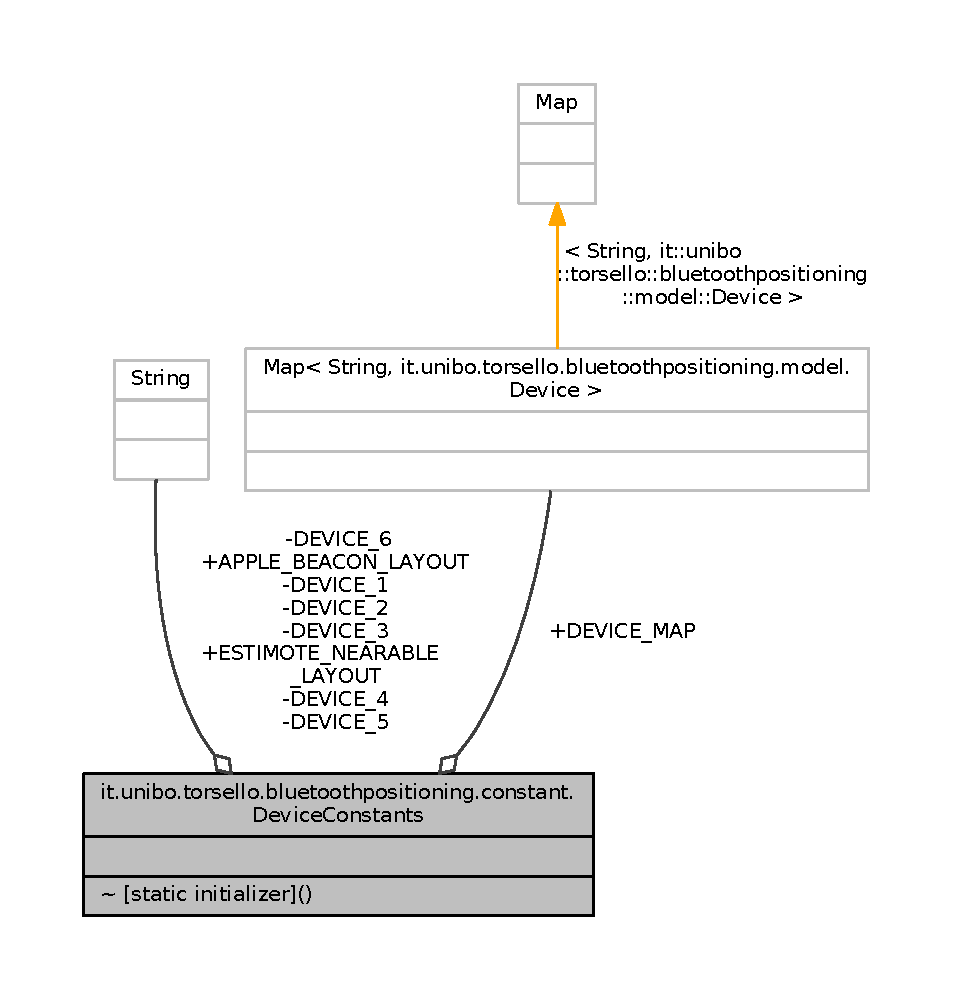
\includegraphics[width=350pt]{classit_1_1unibo_1_1torsello_1_1bluetoothpositioning_1_1constant_1_1DeviceConstants__coll__graph}
\end{center}
\end{figure}
\subsubsection*{Attributi pubblici statici}
\begin{DoxyCompactItemize}
\item 
static final String \hyperlink{classit_1_1unibo_1_1torsello_1_1bluetoothpositioning_1_1constant_1_1DeviceConstants_aceeec7a976dbf40e88728927bec61635_aceeec7a976dbf40e88728927bec61635}{A\+P\+P\+L\+E\+\_\+\+B\+E\+A\+C\+O\+N\+\_\+\+L\+A\+Y\+O\+UT} = \char`\"{}m\+:2-\/3=0215,i\+:4-\/19,i\+:20-\/21,i\+:22-\/23,p\+:24-\/24\char`\"{}
\item 
static final String \hyperlink{classit_1_1unibo_1_1torsello_1_1bluetoothpositioning_1_1constant_1_1DeviceConstants_ac80c3bbd15b47afacffefcdac59e7427_ac80c3bbd15b47afacffefcdac59e7427}{E\+S\+T\+I\+M\+O\+T\+E\+\_\+\+N\+E\+A\+R\+A\+B\+L\+E\+\_\+\+L\+A\+Y\+O\+UT}
\item 
static final Map$<$ String, \hyperlink{classit_1_1unibo_1_1torsello_1_1bluetoothpositioning_1_1model_1_1Device}{Device} $>$ \hyperlink{classit_1_1unibo_1_1torsello_1_1bluetoothpositioning_1_1constant_1_1DeviceConstants_adc3b2d4771c17a3ec55c070dfbe6151a_adc3b2d4771c17a3ec55c070dfbe6151a}{D\+E\+V\+I\+C\+E\+\_\+\+M\+AP}
\end{DoxyCompactItemize}
\subsubsection*{Funzioni statiche con visibilità di package}
\begin{DoxyCompactItemize}
\item 
\hyperlink{classit_1_1unibo_1_1torsello_1_1bluetoothpositioning_1_1constant_1_1DeviceConstants_a99a34b8f281a9d6229cf0adcdc9acd28_a99a34b8f281a9d6229cf0adcdc9acd28}{\mbox{[}static initializer\mbox{]}}
\end{DoxyCompactItemize}
\subsubsection*{Attributi privati statici}
\begin{DoxyCompactItemize}
\item 
static final String \hyperlink{classit_1_1unibo_1_1torsello_1_1bluetoothpositioning_1_1constant_1_1DeviceConstants_a1be810cb4e758baabfa5350f2185b4e1_a1be810cb4e758baabfa5350f2185b4e1}{D\+E\+V\+I\+C\+E\+\_\+1} = \char`\"{}C1\+:9\+B\+:\+B0\+:\+B9\+:01\+:9E\char`\"{}
\item 
static final String \hyperlink{classit_1_1unibo_1_1torsello_1_1bluetoothpositioning_1_1constant_1_1DeviceConstants_a6e71224c86695cf216855bc6c0c77a2d_a6e71224c86695cf216855bc6c0c77a2d}{D\+E\+V\+I\+C\+E\+\_\+2} = \char`\"{}D1\+:\+B\+E\+:\+E2\+:\+E9\+:67\+:\+A6\char`\"{}
\item 
static final String \hyperlink{classit_1_1unibo_1_1torsello_1_1bluetoothpositioning_1_1constant_1_1DeviceConstants_abfaa226793391615faf49ee223f594fb_abfaa226793391615faf49ee223f594fb}{D\+E\+V\+I\+C\+E\+\_\+3} = \char`\"{}F\+A\+:6\+B\+:72\+:1\+E\+:\+E\+B\+:46\char`\"{}
\item 
static final String \hyperlink{classit_1_1unibo_1_1torsello_1_1bluetoothpositioning_1_1constant_1_1DeviceConstants_a77b0930bc8fba094ecdbf42c91d707ea_a77b0930bc8fba094ecdbf42c91d707ea}{D\+E\+V\+I\+C\+E\+\_\+4} = \char`\"{}D9\+:80\+:00\+:\+B7\+:16\+:78\char`\"{}
\item 
static final String \hyperlink{classit_1_1unibo_1_1torsello_1_1bluetoothpositioning_1_1constant_1_1DeviceConstants_a89c9787da5f909162555b4ff956beae4_a89c9787da5f909162555b4ff956beae4}{D\+E\+V\+I\+C\+E\+\_\+5} = \char`\"{}D\+B\+:\+F6\+:\+F5\+:0\+C\+:23\+:\+BF\char`\"{}
\item 
static final String \hyperlink{classit_1_1unibo_1_1torsello_1_1bluetoothpositioning_1_1constant_1_1DeviceConstants_adcdd15d4bd91950603204b771d985527_adcdd15d4bd91950603204b771d985527}{D\+E\+V\+I\+C\+E\+\_\+6} = \char`\"{}E7\+:\+E4\+:0\+E\+:\+F6\+:79\+:3F\char`\"{}
\end{DoxyCompactItemize}


\subsubsection{Descrizione dettagliata}
Created by Federico Torsello. \href{mailto:federico.torsello@studio.unibo.it}{\tt federico.\+torsello@studio.\+unibo.\+it} 

\subsubsection{Documentazione delle funzioni membro}
\hypertarget{classit_1_1unibo_1_1torsello_1_1bluetoothpositioning_1_1constant_1_1DeviceConstants_a99a34b8f281a9d6229cf0adcdc9acd28_a99a34b8f281a9d6229cf0adcdc9acd28}{}\label{classit_1_1unibo_1_1torsello_1_1bluetoothpositioning_1_1constant_1_1DeviceConstants_a99a34b8f281a9d6229cf0adcdc9acd28_a99a34b8f281a9d6229cf0adcdc9acd28} 
\index{it\+::unibo\+::torsello\+::bluetoothpositioning\+::constant\+::\+Device\+Constants@{it\+::unibo\+::torsello\+::bluetoothpositioning\+::constant\+::\+Device\+Constants}!\mbox{[}static initializer\mbox{]}@{[static initializer]}}
\index{\mbox{[}static initializer\mbox{]}@{[static initializer]}!it\+::unibo\+::torsello\+::bluetoothpositioning\+::constant\+::\+Device\+Constants@{it\+::unibo\+::torsello\+::bluetoothpositioning\+::constant\+::\+Device\+Constants}}
\paragraph{\texorpdfstring{[static initializer]()}{[static initializer]()}}
{\footnotesize\ttfamily it.\+unibo.\+torsello.\+bluetoothpositioning.\+constant.\+Device\+Constants.\mbox{[}static initializer\mbox{]} (\begin{DoxyParamCaption}{ }\end{DoxyParamCaption})\hspace{0.3cm}{\ttfamily [static]}, {\ttfamily [package]}}



\subsubsection{Documentazione dei membri dato}
\hypertarget{classit_1_1unibo_1_1torsello_1_1bluetoothpositioning_1_1constant_1_1DeviceConstants_aceeec7a976dbf40e88728927bec61635_aceeec7a976dbf40e88728927bec61635}{}\label{classit_1_1unibo_1_1torsello_1_1bluetoothpositioning_1_1constant_1_1DeviceConstants_aceeec7a976dbf40e88728927bec61635_aceeec7a976dbf40e88728927bec61635} 
\index{it\+::unibo\+::torsello\+::bluetoothpositioning\+::constant\+::\+Device\+Constants@{it\+::unibo\+::torsello\+::bluetoothpositioning\+::constant\+::\+Device\+Constants}!A\+P\+P\+L\+E\+\_\+\+B\+E\+A\+C\+O\+N\+\_\+\+L\+A\+Y\+O\+UT@{A\+P\+P\+L\+E\+\_\+\+B\+E\+A\+C\+O\+N\+\_\+\+L\+A\+Y\+O\+UT}}
\index{A\+P\+P\+L\+E\+\_\+\+B\+E\+A\+C\+O\+N\+\_\+\+L\+A\+Y\+O\+UT@{A\+P\+P\+L\+E\+\_\+\+B\+E\+A\+C\+O\+N\+\_\+\+L\+A\+Y\+O\+UT}!it\+::unibo\+::torsello\+::bluetoothpositioning\+::constant\+::\+Device\+Constants@{it\+::unibo\+::torsello\+::bluetoothpositioning\+::constant\+::\+Device\+Constants}}
\paragraph{\texorpdfstring{A\+P\+P\+L\+E\+\_\+\+B\+E\+A\+C\+O\+N\+\_\+\+L\+A\+Y\+O\+UT}{APPLE\_BEACON\_LAYOUT}}
{\footnotesize\ttfamily final String it.\+unibo.\+torsello.\+bluetoothpositioning.\+constant.\+Device\+Constants.\+A\+P\+P\+L\+E\+\_\+\+B\+E\+A\+C\+O\+N\+\_\+\+L\+A\+Y\+O\+UT = \char`\"{}m\+:2-\/3=0215,i\+:4-\/19,i\+:20-\/21,i\+:22-\/23,p\+:24-\/24\char`\"{}\hspace{0.3cm}{\ttfamily [static]}}

\hypertarget{classit_1_1unibo_1_1torsello_1_1bluetoothpositioning_1_1constant_1_1DeviceConstants_a1be810cb4e758baabfa5350f2185b4e1_a1be810cb4e758baabfa5350f2185b4e1}{}\label{classit_1_1unibo_1_1torsello_1_1bluetoothpositioning_1_1constant_1_1DeviceConstants_a1be810cb4e758baabfa5350f2185b4e1_a1be810cb4e758baabfa5350f2185b4e1} 
\index{it\+::unibo\+::torsello\+::bluetoothpositioning\+::constant\+::\+Device\+Constants@{it\+::unibo\+::torsello\+::bluetoothpositioning\+::constant\+::\+Device\+Constants}!D\+E\+V\+I\+C\+E\+\_\+1@{D\+E\+V\+I\+C\+E\+\_\+1}}
\index{D\+E\+V\+I\+C\+E\+\_\+1@{D\+E\+V\+I\+C\+E\+\_\+1}!it\+::unibo\+::torsello\+::bluetoothpositioning\+::constant\+::\+Device\+Constants@{it\+::unibo\+::torsello\+::bluetoothpositioning\+::constant\+::\+Device\+Constants}}
\paragraph{\texorpdfstring{D\+E\+V\+I\+C\+E\+\_\+1}{DEVICE\_1}}
{\footnotesize\ttfamily final String it.\+unibo.\+torsello.\+bluetoothpositioning.\+constant.\+Device\+Constants.\+D\+E\+V\+I\+C\+E\+\_\+1 = \char`\"{}C1\+:9\+B\+:\+B0\+:\+B9\+:01\+:9E\char`\"{}\hspace{0.3cm}{\ttfamily [static]}, {\ttfamily [private]}}

\hypertarget{classit_1_1unibo_1_1torsello_1_1bluetoothpositioning_1_1constant_1_1DeviceConstants_a6e71224c86695cf216855bc6c0c77a2d_a6e71224c86695cf216855bc6c0c77a2d}{}\label{classit_1_1unibo_1_1torsello_1_1bluetoothpositioning_1_1constant_1_1DeviceConstants_a6e71224c86695cf216855bc6c0c77a2d_a6e71224c86695cf216855bc6c0c77a2d} 
\index{it\+::unibo\+::torsello\+::bluetoothpositioning\+::constant\+::\+Device\+Constants@{it\+::unibo\+::torsello\+::bluetoothpositioning\+::constant\+::\+Device\+Constants}!D\+E\+V\+I\+C\+E\+\_\+2@{D\+E\+V\+I\+C\+E\+\_\+2}}
\index{D\+E\+V\+I\+C\+E\+\_\+2@{D\+E\+V\+I\+C\+E\+\_\+2}!it\+::unibo\+::torsello\+::bluetoothpositioning\+::constant\+::\+Device\+Constants@{it\+::unibo\+::torsello\+::bluetoothpositioning\+::constant\+::\+Device\+Constants}}
\paragraph{\texorpdfstring{D\+E\+V\+I\+C\+E\+\_\+2}{DEVICE\_2}}
{\footnotesize\ttfamily final String it.\+unibo.\+torsello.\+bluetoothpositioning.\+constant.\+Device\+Constants.\+D\+E\+V\+I\+C\+E\+\_\+2 = \char`\"{}D1\+:\+B\+E\+:\+E2\+:\+E9\+:67\+:\+A6\char`\"{}\hspace{0.3cm}{\ttfamily [static]}, {\ttfamily [private]}}

\hypertarget{classit_1_1unibo_1_1torsello_1_1bluetoothpositioning_1_1constant_1_1DeviceConstants_abfaa226793391615faf49ee223f594fb_abfaa226793391615faf49ee223f594fb}{}\label{classit_1_1unibo_1_1torsello_1_1bluetoothpositioning_1_1constant_1_1DeviceConstants_abfaa226793391615faf49ee223f594fb_abfaa226793391615faf49ee223f594fb} 
\index{it\+::unibo\+::torsello\+::bluetoothpositioning\+::constant\+::\+Device\+Constants@{it\+::unibo\+::torsello\+::bluetoothpositioning\+::constant\+::\+Device\+Constants}!D\+E\+V\+I\+C\+E\+\_\+3@{D\+E\+V\+I\+C\+E\+\_\+3}}
\index{D\+E\+V\+I\+C\+E\+\_\+3@{D\+E\+V\+I\+C\+E\+\_\+3}!it\+::unibo\+::torsello\+::bluetoothpositioning\+::constant\+::\+Device\+Constants@{it\+::unibo\+::torsello\+::bluetoothpositioning\+::constant\+::\+Device\+Constants}}
\paragraph{\texorpdfstring{D\+E\+V\+I\+C\+E\+\_\+3}{DEVICE\_3}}
{\footnotesize\ttfamily final String it.\+unibo.\+torsello.\+bluetoothpositioning.\+constant.\+Device\+Constants.\+D\+E\+V\+I\+C\+E\+\_\+3 = \char`\"{}F\+A\+:6\+B\+:72\+:1\+E\+:\+E\+B\+:46\char`\"{}\hspace{0.3cm}{\ttfamily [static]}, {\ttfamily [private]}}

\hypertarget{classit_1_1unibo_1_1torsello_1_1bluetoothpositioning_1_1constant_1_1DeviceConstants_a77b0930bc8fba094ecdbf42c91d707ea_a77b0930bc8fba094ecdbf42c91d707ea}{}\label{classit_1_1unibo_1_1torsello_1_1bluetoothpositioning_1_1constant_1_1DeviceConstants_a77b0930bc8fba094ecdbf42c91d707ea_a77b0930bc8fba094ecdbf42c91d707ea} 
\index{it\+::unibo\+::torsello\+::bluetoothpositioning\+::constant\+::\+Device\+Constants@{it\+::unibo\+::torsello\+::bluetoothpositioning\+::constant\+::\+Device\+Constants}!D\+E\+V\+I\+C\+E\+\_\+4@{D\+E\+V\+I\+C\+E\+\_\+4}}
\index{D\+E\+V\+I\+C\+E\+\_\+4@{D\+E\+V\+I\+C\+E\+\_\+4}!it\+::unibo\+::torsello\+::bluetoothpositioning\+::constant\+::\+Device\+Constants@{it\+::unibo\+::torsello\+::bluetoothpositioning\+::constant\+::\+Device\+Constants}}
\paragraph{\texorpdfstring{D\+E\+V\+I\+C\+E\+\_\+4}{DEVICE\_4}}
{\footnotesize\ttfamily final String it.\+unibo.\+torsello.\+bluetoothpositioning.\+constant.\+Device\+Constants.\+D\+E\+V\+I\+C\+E\+\_\+4 = \char`\"{}D9\+:80\+:00\+:\+B7\+:16\+:78\char`\"{}\hspace{0.3cm}{\ttfamily [static]}, {\ttfamily [private]}}

\hypertarget{classit_1_1unibo_1_1torsello_1_1bluetoothpositioning_1_1constant_1_1DeviceConstants_a89c9787da5f909162555b4ff956beae4_a89c9787da5f909162555b4ff956beae4}{}\label{classit_1_1unibo_1_1torsello_1_1bluetoothpositioning_1_1constant_1_1DeviceConstants_a89c9787da5f909162555b4ff956beae4_a89c9787da5f909162555b4ff956beae4} 
\index{it\+::unibo\+::torsello\+::bluetoothpositioning\+::constant\+::\+Device\+Constants@{it\+::unibo\+::torsello\+::bluetoothpositioning\+::constant\+::\+Device\+Constants}!D\+E\+V\+I\+C\+E\+\_\+5@{D\+E\+V\+I\+C\+E\+\_\+5}}
\index{D\+E\+V\+I\+C\+E\+\_\+5@{D\+E\+V\+I\+C\+E\+\_\+5}!it\+::unibo\+::torsello\+::bluetoothpositioning\+::constant\+::\+Device\+Constants@{it\+::unibo\+::torsello\+::bluetoothpositioning\+::constant\+::\+Device\+Constants}}
\paragraph{\texorpdfstring{D\+E\+V\+I\+C\+E\+\_\+5}{DEVICE\_5}}
{\footnotesize\ttfamily final String it.\+unibo.\+torsello.\+bluetoothpositioning.\+constant.\+Device\+Constants.\+D\+E\+V\+I\+C\+E\+\_\+5 = \char`\"{}D\+B\+:\+F6\+:\+F5\+:0\+C\+:23\+:\+BF\char`\"{}\hspace{0.3cm}{\ttfamily [static]}, {\ttfamily [private]}}

\hypertarget{classit_1_1unibo_1_1torsello_1_1bluetoothpositioning_1_1constant_1_1DeviceConstants_adcdd15d4bd91950603204b771d985527_adcdd15d4bd91950603204b771d985527}{}\label{classit_1_1unibo_1_1torsello_1_1bluetoothpositioning_1_1constant_1_1DeviceConstants_adcdd15d4bd91950603204b771d985527_adcdd15d4bd91950603204b771d985527} 
\index{it\+::unibo\+::torsello\+::bluetoothpositioning\+::constant\+::\+Device\+Constants@{it\+::unibo\+::torsello\+::bluetoothpositioning\+::constant\+::\+Device\+Constants}!D\+E\+V\+I\+C\+E\+\_\+6@{D\+E\+V\+I\+C\+E\+\_\+6}}
\index{D\+E\+V\+I\+C\+E\+\_\+6@{D\+E\+V\+I\+C\+E\+\_\+6}!it\+::unibo\+::torsello\+::bluetoothpositioning\+::constant\+::\+Device\+Constants@{it\+::unibo\+::torsello\+::bluetoothpositioning\+::constant\+::\+Device\+Constants}}
\paragraph{\texorpdfstring{D\+E\+V\+I\+C\+E\+\_\+6}{DEVICE\_6}}
{\footnotesize\ttfamily final String it.\+unibo.\+torsello.\+bluetoothpositioning.\+constant.\+Device\+Constants.\+D\+E\+V\+I\+C\+E\+\_\+6 = \char`\"{}E7\+:\+E4\+:0\+E\+:\+F6\+:79\+:3F\char`\"{}\hspace{0.3cm}{\ttfamily [static]}, {\ttfamily [private]}}

\hypertarget{classit_1_1unibo_1_1torsello_1_1bluetoothpositioning_1_1constant_1_1DeviceConstants_adc3b2d4771c17a3ec55c070dfbe6151a_adc3b2d4771c17a3ec55c070dfbe6151a}{}\label{classit_1_1unibo_1_1torsello_1_1bluetoothpositioning_1_1constant_1_1DeviceConstants_adc3b2d4771c17a3ec55c070dfbe6151a_adc3b2d4771c17a3ec55c070dfbe6151a} 
\index{it\+::unibo\+::torsello\+::bluetoothpositioning\+::constant\+::\+Device\+Constants@{it\+::unibo\+::torsello\+::bluetoothpositioning\+::constant\+::\+Device\+Constants}!D\+E\+V\+I\+C\+E\+\_\+\+M\+AP@{D\+E\+V\+I\+C\+E\+\_\+\+M\+AP}}
\index{D\+E\+V\+I\+C\+E\+\_\+\+M\+AP@{D\+E\+V\+I\+C\+E\+\_\+\+M\+AP}!it\+::unibo\+::torsello\+::bluetoothpositioning\+::constant\+::\+Device\+Constants@{it\+::unibo\+::torsello\+::bluetoothpositioning\+::constant\+::\+Device\+Constants}}
\paragraph{\texorpdfstring{D\+E\+V\+I\+C\+E\+\_\+\+M\+AP}{DEVICE\_MAP}}
{\footnotesize\ttfamily final Map$<$String, \hyperlink{classit_1_1unibo_1_1torsello_1_1bluetoothpositioning_1_1model_1_1Device}{Device}$>$ it.\+unibo.\+torsello.\+bluetoothpositioning.\+constant.\+Device\+Constants.\+D\+E\+V\+I\+C\+E\+\_\+\+M\+AP\hspace{0.3cm}{\ttfamily [static]}}

\hypertarget{classit_1_1unibo_1_1torsello_1_1bluetoothpositioning_1_1constant_1_1DeviceConstants_ac80c3bbd15b47afacffefcdac59e7427_ac80c3bbd15b47afacffefcdac59e7427}{}\label{classit_1_1unibo_1_1torsello_1_1bluetoothpositioning_1_1constant_1_1DeviceConstants_ac80c3bbd15b47afacffefcdac59e7427_ac80c3bbd15b47afacffefcdac59e7427} 
\index{it\+::unibo\+::torsello\+::bluetoothpositioning\+::constant\+::\+Device\+Constants@{it\+::unibo\+::torsello\+::bluetoothpositioning\+::constant\+::\+Device\+Constants}!E\+S\+T\+I\+M\+O\+T\+E\+\_\+\+N\+E\+A\+R\+A\+B\+L\+E\+\_\+\+L\+A\+Y\+O\+UT@{E\+S\+T\+I\+M\+O\+T\+E\+\_\+\+N\+E\+A\+R\+A\+B\+L\+E\+\_\+\+L\+A\+Y\+O\+UT}}
\index{E\+S\+T\+I\+M\+O\+T\+E\+\_\+\+N\+E\+A\+R\+A\+B\+L\+E\+\_\+\+L\+A\+Y\+O\+UT@{E\+S\+T\+I\+M\+O\+T\+E\+\_\+\+N\+E\+A\+R\+A\+B\+L\+E\+\_\+\+L\+A\+Y\+O\+UT}!it\+::unibo\+::torsello\+::bluetoothpositioning\+::constant\+::\+Device\+Constants@{it\+::unibo\+::torsello\+::bluetoothpositioning\+::constant\+::\+Device\+Constants}}
\paragraph{\texorpdfstring{E\+S\+T\+I\+M\+O\+T\+E\+\_\+\+N\+E\+A\+R\+A\+B\+L\+E\+\_\+\+L\+A\+Y\+O\+UT}{ESTIMOTE\_NEARABLE\_LAYOUT}}
{\footnotesize\ttfamily final String it.\+unibo.\+torsello.\+bluetoothpositioning.\+constant.\+Device\+Constants.\+E\+S\+T\+I\+M\+O\+T\+E\+\_\+\+N\+E\+A\+R\+A\+B\+L\+E\+\_\+\+L\+A\+Y\+O\+UT\hspace{0.3cm}{\ttfamily [static]}}

{\bfseries Valore iniziale\+:}
\begin{DoxyCode}
= \textcolor{stringliteral}{"m:1-2=0101,i:3-10,d:11-11,d:12-12,"} +
            \textcolor{stringliteral}{"d:13-14,d:15-15,d:16-16,d:17-17,d:18-18,d:19-19,d:20-20, p:21-21"}
\end{DoxyCode}


La documentazione per questa classe è stata generata a partire dal seguente file\+:\begin{DoxyCompactItemize}
\item 
\hyperlink{DeviceConstants_8java}{Device\+Constants.\+java}\end{DoxyCompactItemize}

\hypertarget{classit_1_1unibo_1_1torsello_1_1bluetoothpositioning_1_1fragment_1_1DeviceDetailFragment}{}\subsection{Riferimenti per la classe it.\+unibo.\+torsello.\+bluetoothpositioning.\+fragment.\+Device\+Detail\+Fragment}
\label{classit_1_1unibo_1_1torsello_1_1bluetoothpositioning_1_1fragment_1_1DeviceDetailFragment}\index{it.\+unibo.\+torsello.\+bluetoothpositioning.\+fragment.\+Device\+Detail\+Fragment@{it.\+unibo.\+torsello.\+bluetoothpositioning.\+fragment.\+Device\+Detail\+Fragment}}


Diagramma delle classi per it.\+unibo.\+torsello.\+bluetoothpositioning.\+fragment.\+Device\+Detail\+Fragment
\nopagebreak
\begin{figure}[H]
\begin{center}
\leavevmode
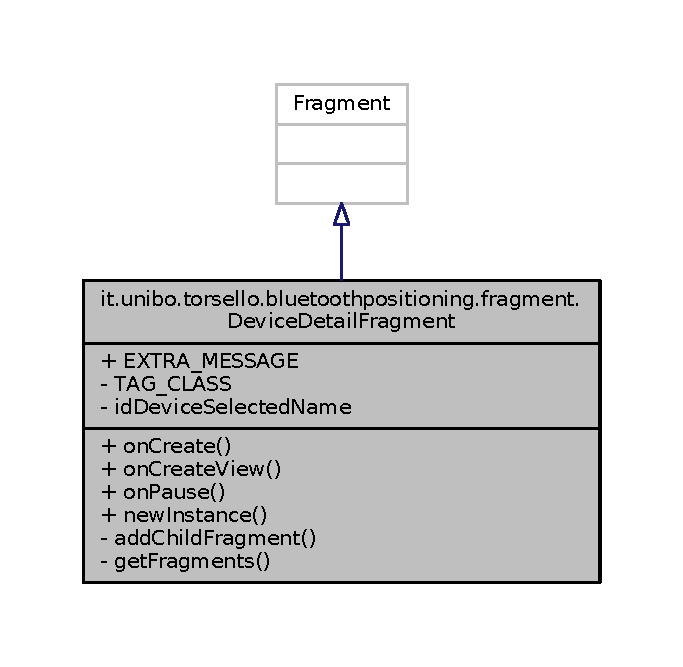
\includegraphics[width=328pt]{classit_1_1unibo_1_1torsello_1_1bluetoothpositioning_1_1fragment_1_1DeviceDetailFragment__inherit__graph}
\end{center}
\end{figure}


Diagramma di collaborazione per it.\+unibo.\+torsello.\+bluetoothpositioning.\+fragment.\+Device\+Detail\+Fragment\+:
\nopagebreak
\begin{figure}[H]
\begin{center}
\leavevmode
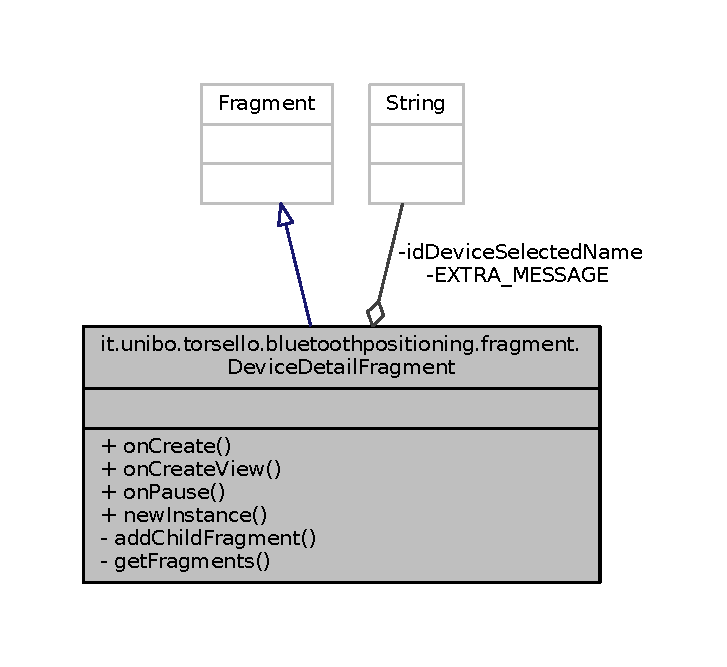
\includegraphics[width=349pt]{classit_1_1unibo_1_1torsello_1_1bluetoothpositioning_1_1fragment_1_1DeviceDetailFragment__coll__graph}
\end{center}
\end{figure}
\subsubsection*{Membri pubblici}
\begin{DoxyCompactItemize}
\item 
void \hyperlink{classit_1_1unibo_1_1torsello_1_1bluetoothpositioning_1_1fragment_1_1DeviceDetailFragment_af33d782c107be10fe752f16f04cc5e5d_af33d782c107be10fe752f16f04cc5e5d}{on\+Create} (Bundle saved\+Instance\+State)
\item 
View \hyperlink{classit_1_1unibo_1_1torsello_1_1bluetoothpositioning_1_1fragment_1_1DeviceDetailFragment_a6d43be281b577e0d9f2540fea30c2fdf_a6d43be281b577e0d9f2540fea30c2fdf}{on\+Create\+View} (Layout\+Inflater inflater, View\+Group container, Bundle saved\+Instance\+State)
\item 
void \hyperlink{classit_1_1unibo_1_1torsello_1_1bluetoothpositioning_1_1fragment_1_1DeviceDetailFragment_a1ed4762356dd3067ce48aa73da50404e_a1ed4762356dd3067ce48aa73da50404e}{on\+Pause} ()
\end{DoxyCompactItemize}
\subsubsection*{Membri pubblici statici}
\begin{DoxyCompactItemize}
\item 
static \hyperlink{classit_1_1unibo_1_1torsello_1_1bluetoothpositioning_1_1fragment_1_1DeviceDetailFragment}{Device\+Detail\+Fragment} \hyperlink{classit_1_1unibo_1_1torsello_1_1bluetoothpositioning_1_1fragment_1_1DeviceDetailFragment_a626de18d36d44ae0b4ff21c2527bdf5a_a626de18d36d44ae0b4ff21c2527bdf5a}{new\+Instance} (String message)
\end{DoxyCompactItemize}
\subsubsection*{Membri privati}
\begin{DoxyCompactItemize}
\item 
void \hyperlink{classit_1_1unibo_1_1torsello_1_1bluetoothpositioning_1_1fragment_1_1DeviceDetailFragment_a62c541b8382a522f06a5d9c56cf50b26_a62c541b8382a522f06a5d9c56cf50b26}{add\+Child\+Fragment} (View root)
\item 
Array\+List$<$ Fragment $>$ \hyperlink{classit_1_1unibo_1_1torsello_1_1bluetoothpositioning_1_1fragment_1_1DeviceDetailFragment_a98e370cfcbfe5eaa4e1fe9242b00e639_a98e370cfcbfe5eaa4e1fe9242b00e639}{get\+Fragments} ()
\end{DoxyCompactItemize}
\subsubsection*{Attributi privati}
\begin{DoxyCompactItemize}
\item 
String \hyperlink{classit_1_1unibo_1_1torsello_1_1bluetoothpositioning_1_1fragment_1_1DeviceDetailFragment_a6d52d8371a07fb8da75879758d1d6942_a6d52d8371a07fb8da75879758d1d6942}{id\+Device\+Selected\+Name}
\end{DoxyCompactItemize}
\subsubsection*{Attributi privati statici}
\begin{DoxyCompactItemize}
\item 
static final String \hyperlink{classit_1_1unibo_1_1torsello_1_1bluetoothpositioning_1_1fragment_1_1DeviceDetailFragment_a9f7fff4a2b22105976f2c7223d88f9ae_a9f7fff4a2b22105976f2c7223d88f9ae}{E\+X\+T\+R\+A\+\_\+\+M\+E\+S\+S\+A\+GE} = \char`\"{}E\+X\+T\+R\+A\+\_\+\+M\+E\+S\+S\+A\+GE\char`\"{}
\end{DoxyCompactItemize}


\subsubsection{Descrizione dettagliata}
Created by Federico Torsello. \href{mailto:federico.torsello@studio.unibo.it}{\tt federico.\+torsello@studio.\+unibo.\+it} 

\subsubsection{Documentazione delle funzioni membro}
\hypertarget{classit_1_1unibo_1_1torsello_1_1bluetoothpositioning_1_1fragment_1_1DeviceDetailFragment_a62c541b8382a522f06a5d9c56cf50b26_a62c541b8382a522f06a5d9c56cf50b26}{}\label{classit_1_1unibo_1_1torsello_1_1bluetoothpositioning_1_1fragment_1_1DeviceDetailFragment_a62c541b8382a522f06a5d9c56cf50b26_a62c541b8382a522f06a5d9c56cf50b26} 
\index{it\+::unibo\+::torsello\+::bluetoothpositioning\+::fragment\+::\+Device\+Detail\+Fragment@{it\+::unibo\+::torsello\+::bluetoothpositioning\+::fragment\+::\+Device\+Detail\+Fragment}!add\+Child\+Fragment@{add\+Child\+Fragment}}
\index{add\+Child\+Fragment@{add\+Child\+Fragment}!it\+::unibo\+::torsello\+::bluetoothpositioning\+::fragment\+::\+Device\+Detail\+Fragment@{it\+::unibo\+::torsello\+::bluetoothpositioning\+::fragment\+::\+Device\+Detail\+Fragment}}
\paragraph{\texorpdfstring{add\+Child\+Fragment()}{addChildFragment()}}
{\footnotesize\ttfamily void it.\+unibo.\+torsello.\+bluetoothpositioning.\+fragment.\+Device\+Detail\+Fragment.\+add\+Child\+Fragment (\begin{DoxyParamCaption}\item[{View}]{root }\end{DoxyParamCaption})\hspace{0.3cm}{\ttfamily [private]}}


\begin{DoxyCode}
63                                              \{
64 
65         ViewPager mViewPager = (ViewPager) root.findViewById(R.id.view\_pager);
66         StatePagerAdapter myPageAdapter = \textcolor{keyword}{new} StatePagerAdapter(getChildFragmentManager(), 
      \hyperlink{classit_1_1unibo_1_1torsello_1_1bluetoothpositioning_1_1fragment_1_1DeviceDetailFragment_a98e370cfcbfe5eaa4e1fe9242b00e639_a98e370cfcbfe5eaa4e1fe9242b00e639}{getFragments}());
67         mViewPager.setAdapter(myPageAdapter);
68 
69         TabLayout tabLayout = (TabLayout) root.findViewById(R.id.sliding\_tabs);
70         tabLayout.setupWithViewPager(mViewPager);
71     \}
\end{DoxyCode}
\hypertarget{classit_1_1unibo_1_1torsello_1_1bluetoothpositioning_1_1fragment_1_1DeviceDetailFragment_a98e370cfcbfe5eaa4e1fe9242b00e639_a98e370cfcbfe5eaa4e1fe9242b00e639}{}\label{classit_1_1unibo_1_1torsello_1_1bluetoothpositioning_1_1fragment_1_1DeviceDetailFragment_a98e370cfcbfe5eaa4e1fe9242b00e639_a98e370cfcbfe5eaa4e1fe9242b00e639} 
\index{it\+::unibo\+::torsello\+::bluetoothpositioning\+::fragment\+::\+Device\+Detail\+Fragment@{it\+::unibo\+::torsello\+::bluetoothpositioning\+::fragment\+::\+Device\+Detail\+Fragment}!get\+Fragments@{get\+Fragments}}
\index{get\+Fragments@{get\+Fragments}!it\+::unibo\+::torsello\+::bluetoothpositioning\+::fragment\+::\+Device\+Detail\+Fragment@{it\+::unibo\+::torsello\+::bluetoothpositioning\+::fragment\+::\+Device\+Detail\+Fragment}}
\paragraph{\texorpdfstring{get\+Fragments()}{getFragments()}}
{\footnotesize\ttfamily Array\+List$<$Fragment$>$ it.\+unibo.\+torsello.\+bluetoothpositioning.\+fragment.\+Device\+Detail\+Fragment.\+get\+Fragments (\begin{DoxyParamCaption}{ }\end{DoxyParamCaption})\hspace{0.3cm}{\ttfamily [private]}}


\begin{DoxyCode}
73                                                \{
74 
75         ArrayList<Fragment> fragments = \textcolor{keyword}{new} ArrayList<>();
76 
77         \textcolor{comment}{// fragment 0}
78         fragments.add(DeviceDetailInner1Fragment.newInstance(
      \hyperlink{classit_1_1unibo_1_1torsello_1_1bluetoothpositioning_1_1fragment_1_1DeviceDetailFragment_a6d52d8371a07fb8da75879758d1d6942_a6d52d8371a07fb8da75879758d1d6942}{idDeviceSelectedName}));
79 
80         \textcolor{comment}{// fragment 1}
81         fragments.add(DeviceDetailInner2Fragment.newInstance(\textcolor{stringliteral}{"Details"}, 
      \hyperlink{classit_1_1unibo_1_1torsello_1_1bluetoothpositioning_1_1fragment_1_1DeviceDetailFragment_a6d52d8371a07fb8da75879758d1d6942_a6d52d8371a07fb8da75879758d1d6942}{idDeviceSelectedName}));
82 
83 
84         \textcolor{keywordflow}{return} fragments;
85     \}
\end{DoxyCode}
\hypertarget{classit_1_1unibo_1_1torsello_1_1bluetoothpositioning_1_1fragment_1_1DeviceDetailFragment_a626de18d36d44ae0b4ff21c2527bdf5a_a626de18d36d44ae0b4ff21c2527bdf5a}{}\label{classit_1_1unibo_1_1torsello_1_1bluetoothpositioning_1_1fragment_1_1DeviceDetailFragment_a626de18d36d44ae0b4ff21c2527bdf5a_a626de18d36d44ae0b4ff21c2527bdf5a} 
\index{it\+::unibo\+::torsello\+::bluetoothpositioning\+::fragment\+::\+Device\+Detail\+Fragment@{it\+::unibo\+::torsello\+::bluetoothpositioning\+::fragment\+::\+Device\+Detail\+Fragment}!new\+Instance@{new\+Instance}}
\index{new\+Instance@{new\+Instance}!it\+::unibo\+::torsello\+::bluetoothpositioning\+::fragment\+::\+Device\+Detail\+Fragment@{it\+::unibo\+::torsello\+::bluetoothpositioning\+::fragment\+::\+Device\+Detail\+Fragment}}
\paragraph{\texorpdfstring{new\+Instance()}{newInstance()}}
{\footnotesize\ttfamily static \hyperlink{classit_1_1unibo_1_1torsello_1_1bluetoothpositioning_1_1fragment_1_1DeviceDetailFragment}{Device\+Detail\+Fragment} it.\+unibo.\+torsello.\+bluetoothpositioning.\+fragment.\+Device\+Detail\+Fragment.\+new\+Instance (\begin{DoxyParamCaption}\item[{String}]{message }\end{DoxyParamCaption})\hspace{0.3cm}{\ttfamily [static]}}


\begin{DoxyCode}
29                                                                    \{
30         DeviceDetailFragment fragment = \textcolor{keyword}{new} DeviceDetailFragment();
31         Bundle args = \textcolor{keyword}{new} Bundle();
32         args.putString(\hyperlink{classit_1_1unibo_1_1torsello_1_1bluetoothpositioning_1_1fragment_1_1DeviceDetailFragment_a9f7fff4a2b22105976f2c7223d88f9ae_a9f7fff4a2b22105976f2c7223d88f9ae}{EXTRA\_MESSAGE}, message);
33         fragment.setArguments(args);
34         \textcolor{keywordflow}{return} fragment;
35     \}
\end{DoxyCode}
\hypertarget{classit_1_1unibo_1_1torsello_1_1bluetoothpositioning_1_1fragment_1_1DeviceDetailFragment_af33d782c107be10fe752f16f04cc5e5d_af33d782c107be10fe752f16f04cc5e5d}{}\label{classit_1_1unibo_1_1torsello_1_1bluetoothpositioning_1_1fragment_1_1DeviceDetailFragment_af33d782c107be10fe752f16f04cc5e5d_af33d782c107be10fe752f16f04cc5e5d} 
\index{it\+::unibo\+::torsello\+::bluetoothpositioning\+::fragment\+::\+Device\+Detail\+Fragment@{it\+::unibo\+::torsello\+::bluetoothpositioning\+::fragment\+::\+Device\+Detail\+Fragment}!on\+Create@{on\+Create}}
\index{on\+Create@{on\+Create}!it\+::unibo\+::torsello\+::bluetoothpositioning\+::fragment\+::\+Device\+Detail\+Fragment@{it\+::unibo\+::torsello\+::bluetoothpositioning\+::fragment\+::\+Device\+Detail\+Fragment}}
\paragraph{\texorpdfstring{on\+Create()}{onCreate()}}
{\footnotesize\ttfamily void it.\+unibo.\+torsello.\+bluetoothpositioning.\+fragment.\+Device\+Detail\+Fragment.\+on\+Create (\begin{DoxyParamCaption}\item[{Bundle}]{saved\+Instance\+State }\end{DoxyParamCaption})}


\begin{DoxyCode}
38                                                     \{
39         super.onCreate(savedInstanceState);
40 
41         \hyperlink{classit_1_1unibo_1_1torsello_1_1bluetoothpositioning_1_1fragment_1_1DeviceDetailFragment_a6d52d8371a07fb8da75879758d1d6942_a6d52d8371a07fb8da75879758d1d6942}{idDeviceSelectedName} = getArguments().getString(
      \hyperlink{classit_1_1unibo_1_1torsello_1_1bluetoothpositioning_1_1fragment_1_1DeviceDetailFragment_a9f7fff4a2b22105976f2c7223d88f9ae_a9f7fff4a2b22105976f2c7223d88f9ae}{EXTRA\_MESSAGE});
42     \}
\end{DoxyCode}
\hypertarget{classit_1_1unibo_1_1torsello_1_1bluetoothpositioning_1_1fragment_1_1DeviceDetailFragment_a6d43be281b577e0d9f2540fea30c2fdf_a6d43be281b577e0d9f2540fea30c2fdf}{}\label{classit_1_1unibo_1_1torsello_1_1bluetoothpositioning_1_1fragment_1_1DeviceDetailFragment_a6d43be281b577e0d9f2540fea30c2fdf_a6d43be281b577e0d9f2540fea30c2fdf} 
\index{it\+::unibo\+::torsello\+::bluetoothpositioning\+::fragment\+::\+Device\+Detail\+Fragment@{it\+::unibo\+::torsello\+::bluetoothpositioning\+::fragment\+::\+Device\+Detail\+Fragment}!on\+Create\+View@{on\+Create\+View}}
\index{on\+Create\+View@{on\+Create\+View}!it\+::unibo\+::torsello\+::bluetoothpositioning\+::fragment\+::\+Device\+Detail\+Fragment@{it\+::unibo\+::torsello\+::bluetoothpositioning\+::fragment\+::\+Device\+Detail\+Fragment}}
\paragraph{\texorpdfstring{on\+Create\+View()}{onCreateView()}}
{\footnotesize\ttfamily View it.\+unibo.\+torsello.\+bluetoothpositioning.\+fragment.\+Device\+Detail\+Fragment.\+on\+Create\+View (\begin{DoxyParamCaption}\item[{Layout\+Inflater}]{inflater,  }\item[{View\+Group}]{container,  }\item[{Bundle}]{saved\+Instance\+State }\end{DoxyParamCaption})}


\begin{DoxyCode}
45                                                                                                       \{
46         \textcolor{keyword}{final} View root = inflater.inflate(R.layout.fragment\_device\_detail, container, \textcolor{keyword}{false});
47 
48         getActivity().findViewById(R.id.toolbar).setVisibility(View.GONE);
49 
50         ((AppBarLayout) root.findViewById(R.id.appbar\_detail)).setExpanded(\textcolor{keyword}{false});
51         ((CollapsingToolbarLayout) root.findViewById(R.id.collapsing\_toolbar)).setTitle(
      \hyperlink{classit_1_1unibo_1_1torsello_1_1bluetoothpositioning_1_1fragment_1_1DeviceDetailFragment_a6d52d8371a07fb8da75879758d1d6942_a6d52d8371a07fb8da75879758d1d6942}{idDeviceSelectedName});
52 
53         \hyperlink{classit_1_1unibo_1_1torsello_1_1bluetoothpositioning_1_1fragment_1_1DeviceDetailFragment_a62c541b8382a522f06a5d9c56cf50b26_a62c541b8382a522f06a5d9c56cf50b26}{addChildFragment}(root);
54         \textcolor{keywordflow}{return} root;
55     \}
\end{DoxyCode}
\hypertarget{classit_1_1unibo_1_1torsello_1_1bluetoothpositioning_1_1fragment_1_1DeviceDetailFragment_a1ed4762356dd3067ce48aa73da50404e_a1ed4762356dd3067ce48aa73da50404e}{}\label{classit_1_1unibo_1_1torsello_1_1bluetoothpositioning_1_1fragment_1_1DeviceDetailFragment_a1ed4762356dd3067ce48aa73da50404e_a1ed4762356dd3067ce48aa73da50404e} 
\index{it\+::unibo\+::torsello\+::bluetoothpositioning\+::fragment\+::\+Device\+Detail\+Fragment@{it\+::unibo\+::torsello\+::bluetoothpositioning\+::fragment\+::\+Device\+Detail\+Fragment}!on\+Pause@{on\+Pause}}
\index{on\+Pause@{on\+Pause}!it\+::unibo\+::torsello\+::bluetoothpositioning\+::fragment\+::\+Device\+Detail\+Fragment@{it\+::unibo\+::torsello\+::bluetoothpositioning\+::fragment\+::\+Device\+Detail\+Fragment}}
\paragraph{\texorpdfstring{on\+Pause()}{onPause()}}
{\footnotesize\ttfamily void it.\+unibo.\+torsello.\+bluetoothpositioning.\+fragment.\+Device\+Detail\+Fragment.\+on\+Pause (\begin{DoxyParamCaption}{ }\end{DoxyParamCaption})}


\begin{DoxyCode}
58                           \{
59         getActivity().findViewById(R.id.toolbar).setVisibility(View.VISIBLE);
60         super.onPause();
61     \}
\end{DoxyCode}


\subsubsection{Documentazione dei membri dato}
\hypertarget{classit_1_1unibo_1_1torsello_1_1bluetoothpositioning_1_1fragment_1_1DeviceDetailFragment_a9f7fff4a2b22105976f2c7223d88f9ae_a9f7fff4a2b22105976f2c7223d88f9ae}{}\label{classit_1_1unibo_1_1torsello_1_1bluetoothpositioning_1_1fragment_1_1DeviceDetailFragment_a9f7fff4a2b22105976f2c7223d88f9ae_a9f7fff4a2b22105976f2c7223d88f9ae} 
\index{it\+::unibo\+::torsello\+::bluetoothpositioning\+::fragment\+::\+Device\+Detail\+Fragment@{it\+::unibo\+::torsello\+::bluetoothpositioning\+::fragment\+::\+Device\+Detail\+Fragment}!E\+X\+T\+R\+A\+\_\+\+M\+E\+S\+S\+A\+GE@{E\+X\+T\+R\+A\+\_\+\+M\+E\+S\+S\+A\+GE}}
\index{E\+X\+T\+R\+A\+\_\+\+M\+E\+S\+S\+A\+GE@{E\+X\+T\+R\+A\+\_\+\+M\+E\+S\+S\+A\+GE}!it\+::unibo\+::torsello\+::bluetoothpositioning\+::fragment\+::\+Device\+Detail\+Fragment@{it\+::unibo\+::torsello\+::bluetoothpositioning\+::fragment\+::\+Device\+Detail\+Fragment}}
\paragraph{\texorpdfstring{E\+X\+T\+R\+A\+\_\+\+M\+E\+S\+S\+A\+GE}{EXTRA\_MESSAGE}}
{\footnotesize\ttfamily final String it.\+unibo.\+torsello.\+bluetoothpositioning.\+fragment.\+Device\+Detail\+Fragment.\+E\+X\+T\+R\+A\+\_\+\+M\+E\+S\+S\+A\+GE = \char`\"{}E\+X\+T\+R\+A\+\_\+\+M\+E\+S\+S\+A\+GE\char`\"{}\hspace{0.3cm}{\ttfamily [static]}, {\ttfamily [private]}}

\hypertarget{classit_1_1unibo_1_1torsello_1_1bluetoothpositioning_1_1fragment_1_1DeviceDetailFragment_a6d52d8371a07fb8da75879758d1d6942_a6d52d8371a07fb8da75879758d1d6942}{}\label{classit_1_1unibo_1_1torsello_1_1bluetoothpositioning_1_1fragment_1_1DeviceDetailFragment_a6d52d8371a07fb8da75879758d1d6942_a6d52d8371a07fb8da75879758d1d6942} 
\index{it\+::unibo\+::torsello\+::bluetoothpositioning\+::fragment\+::\+Device\+Detail\+Fragment@{it\+::unibo\+::torsello\+::bluetoothpositioning\+::fragment\+::\+Device\+Detail\+Fragment}!id\+Device\+Selected\+Name@{id\+Device\+Selected\+Name}}
\index{id\+Device\+Selected\+Name@{id\+Device\+Selected\+Name}!it\+::unibo\+::torsello\+::bluetoothpositioning\+::fragment\+::\+Device\+Detail\+Fragment@{it\+::unibo\+::torsello\+::bluetoothpositioning\+::fragment\+::\+Device\+Detail\+Fragment}}
\paragraph{\texorpdfstring{id\+Device\+Selected\+Name}{idDeviceSelectedName}}
{\footnotesize\ttfamily String it.\+unibo.\+torsello.\+bluetoothpositioning.\+fragment.\+Device\+Detail\+Fragment.\+id\+Device\+Selected\+Name\hspace{0.3cm}{\ttfamily [private]}}



La documentazione per questa classe è stata generata a partire dal seguente file\+:\begin{DoxyCompactItemize}
\item 
\hyperlink{DeviceDetailFragment_8java}{Device\+Detail\+Fragment.\+java}\end{DoxyCompactItemize}

\hypertarget{classit_1_1unibo_1_1torsello_1_1bluetoothpositioning_1_1fragment_1_1DeviceDetailInner0Fragment}{}\subsection{Riferimenti per la classe it.\+unibo.\+torsello.\+bluetoothpositioning.\+fragment.\+Device\+Detail\+Inner0\+Fragment}
\label{classit_1_1unibo_1_1torsello_1_1bluetoothpositioning_1_1fragment_1_1DeviceDetailInner0Fragment}\index{it.\+unibo.\+torsello.\+bluetoothpositioning.\+fragment.\+Device\+Detail\+Inner0\+Fragment@{it.\+unibo.\+torsello.\+bluetoothpositioning.\+fragment.\+Device\+Detail\+Inner0\+Fragment}}


Diagramma delle classi per it.\+unibo.\+torsello.\+bluetoothpositioning.\+fragment.\+Device\+Detail\+Inner0\+Fragment
\nopagebreak
\begin{figure}[H]
\begin{center}
\leavevmode
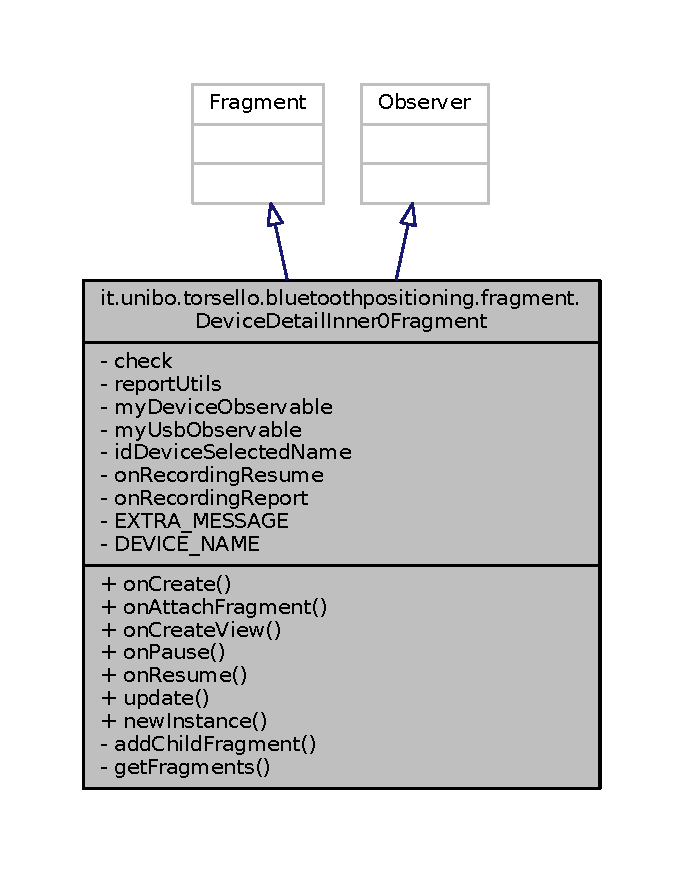
\includegraphics[width=328pt]{classit_1_1unibo_1_1torsello_1_1bluetoothpositioning_1_1fragment_1_1DeviceDetailInner0Fragment__inherit__graph}
\end{center}
\end{figure}


Diagramma di collaborazione per it.\+unibo.\+torsello.\+bluetoothpositioning.\+fragment.\+Device\+Detail\+Inner0\+Fragment\+:
\nopagebreak
\begin{figure}[H]
\begin{center}
\leavevmode
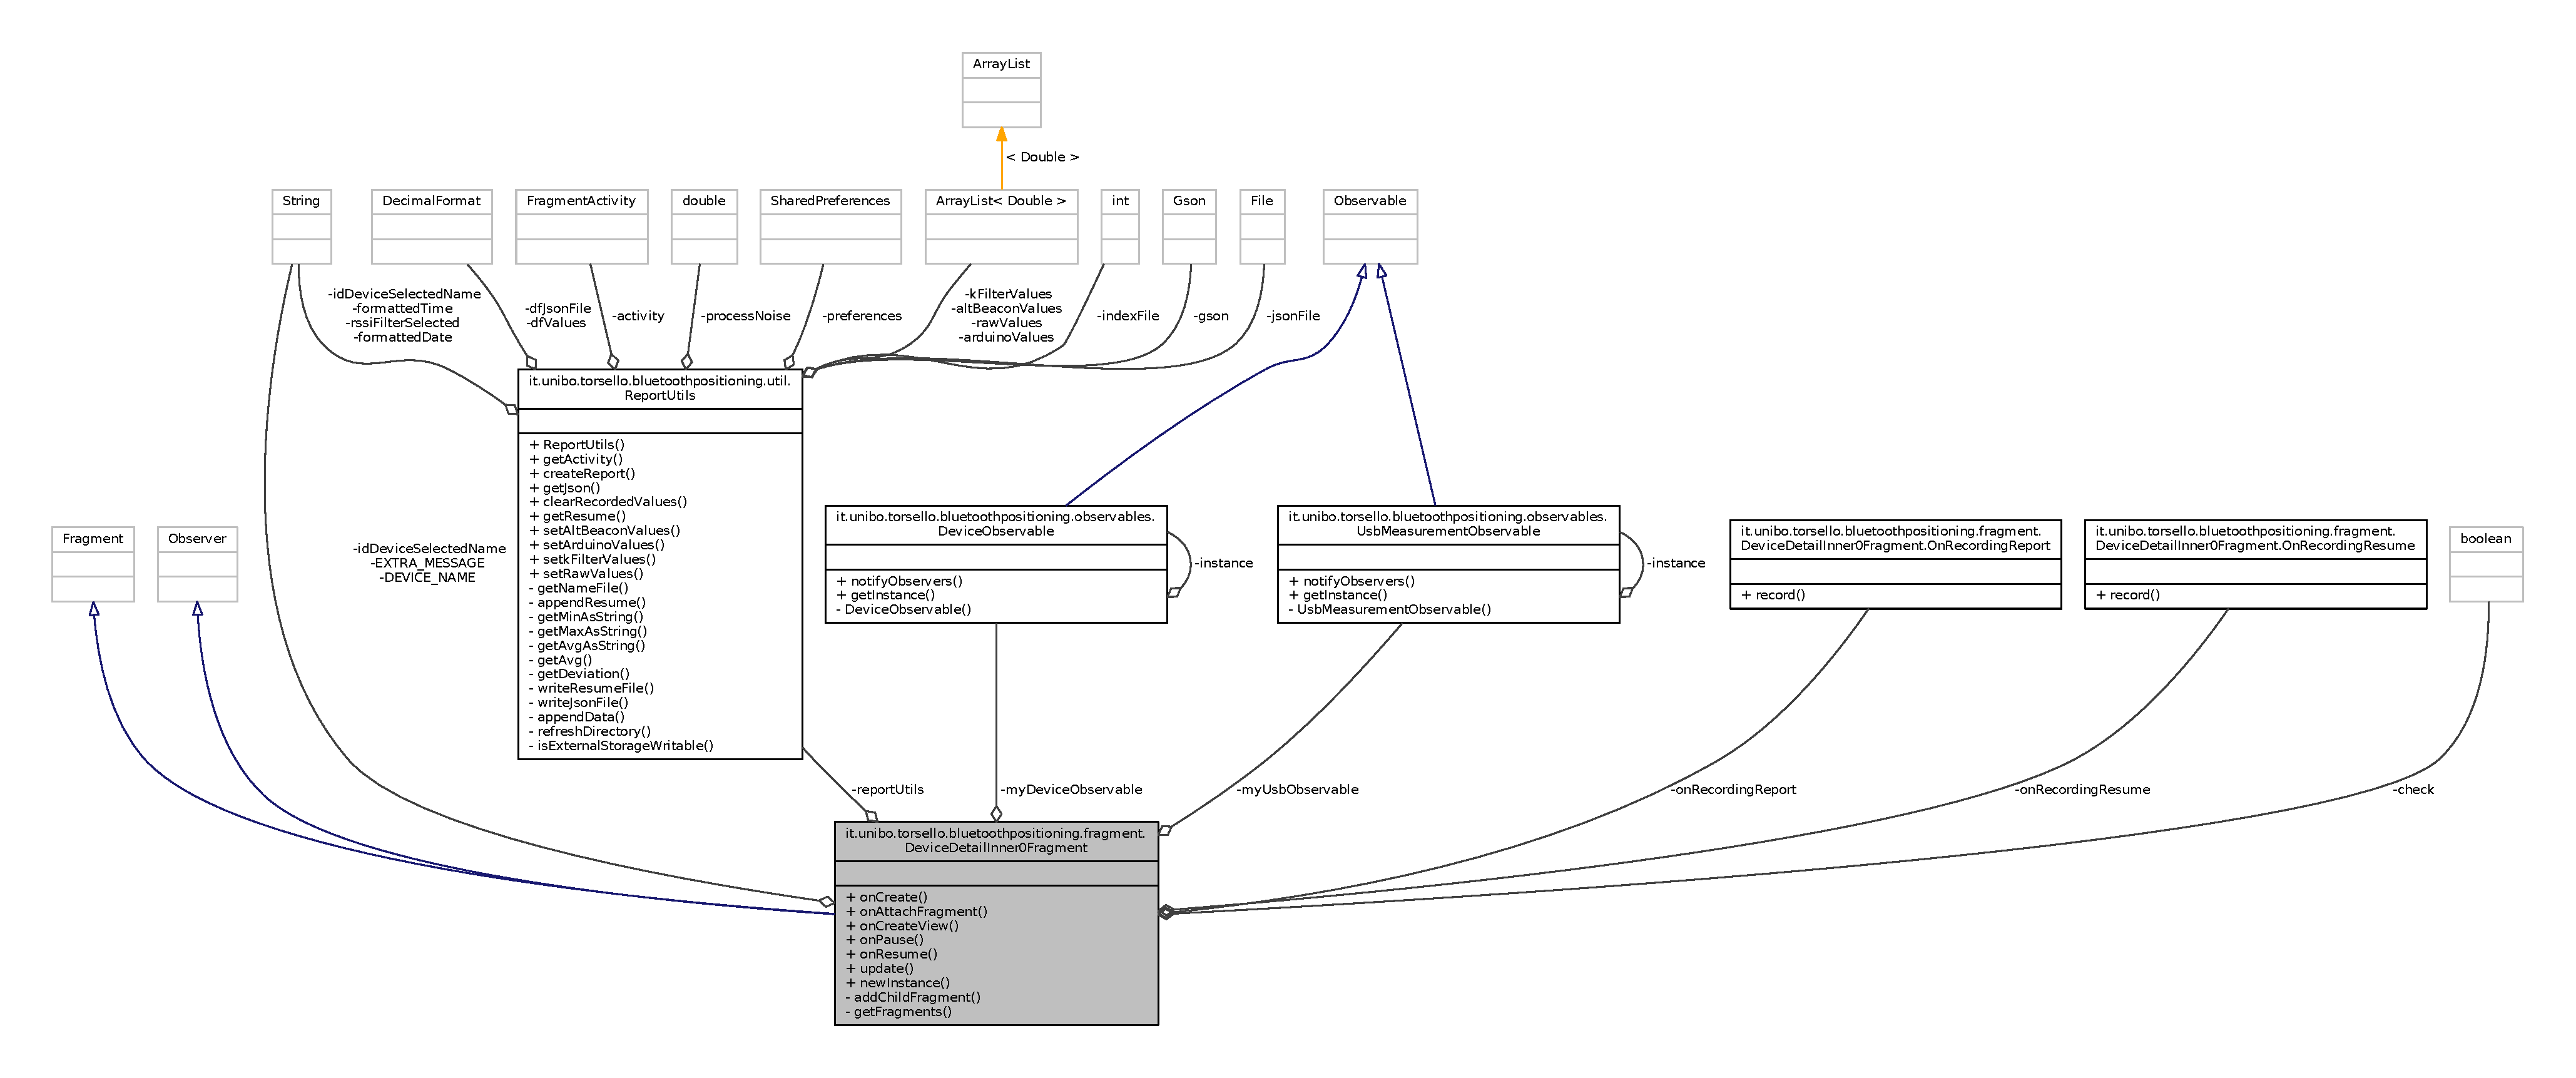
\includegraphics[width=350pt]{classit_1_1unibo_1_1torsello_1_1bluetoothpositioning_1_1fragment_1_1DeviceDetailInner0Fragment__coll__graph}
\end{center}
\end{figure}
\subsubsection*{Composti}
\begin{DoxyCompactItemize}
\item 
interface \hyperlink{interfaceit_1_1unibo_1_1torsello_1_1bluetoothpositioning_1_1fragment_1_1DeviceDetailInner0Fragment_1_1OnRecordingReport}{On\+Recording\+Report}
\item 
interface \hyperlink{interfaceit_1_1unibo_1_1torsello_1_1bluetoothpositioning_1_1fragment_1_1DeviceDetailInner0Fragment_1_1OnRecordingResume}{On\+Recording\+Resume}
\end{DoxyCompactItemize}
\subsubsection*{Membri pubblici}
\begin{DoxyCompactItemize}
\item 
void \hyperlink{classit_1_1unibo_1_1torsello_1_1bluetoothpositioning_1_1fragment_1_1DeviceDetailInner0Fragment_a799f69a27b82be0bf972611b1743e8bd_a799f69a27b82be0bf972611b1743e8bd}{on\+Create} (Bundle saved\+Instance\+State)
\item 
void \hyperlink{classit_1_1unibo_1_1torsello_1_1bluetoothpositioning_1_1fragment_1_1DeviceDetailInner0Fragment_a0893d44029c05595acc4cbe5bb458772_a0893d44029c05595acc4cbe5bb458772}{on\+Attach\+Fragment} (Fragment child\+Fragment)
\item 
View \hyperlink{classit_1_1unibo_1_1torsello_1_1bluetoothpositioning_1_1fragment_1_1DeviceDetailInner0Fragment_a7a1163483f1abdefe3f08bcd67ff4f08_a7a1163483f1abdefe3f08bcd67ff4f08}{on\+Create\+View} (Layout\+Inflater inflater, View\+Group container, Bundle saved\+Instance\+State)
\item 
void \hyperlink{classit_1_1unibo_1_1torsello_1_1bluetoothpositioning_1_1fragment_1_1DeviceDetailInner0Fragment_a8fc220176497363521dd4b0b190e4c49_a8fc220176497363521dd4b0b190e4c49}{on\+Pause} ()
\item 
void \hyperlink{classit_1_1unibo_1_1torsello_1_1bluetoothpositioning_1_1fragment_1_1DeviceDetailInner0Fragment_a2ccd1bfbb26e6896ccdbeb4eb4c6adcb_a2ccd1bfbb26e6896ccdbeb4eb4c6adcb}{on\+Resume} ()
\item 
void \hyperlink{classit_1_1unibo_1_1torsello_1_1bluetoothpositioning_1_1fragment_1_1DeviceDetailInner0Fragment_aa80acc0e82730a27b0085e5da3087d20_aa80acc0e82730a27b0085e5da3087d20}{update} (Observable observable, Object arg)
\end{DoxyCompactItemize}
\subsubsection*{Membri pubblici statici}
\begin{DoxyCompactItemize}
\item 
static \hyperlink{classit_1_1unibo_1_1torsello_1_1bluetoothpositioning_1_1fragment_1_1DeviceDetailInner0Fragment}{Device\+Detail\+Inner0\+Fragment} \hyperlink{classit_1_1unibo_1_1torsello_1_1bluetoothpositioning_1_1fragment_1_1DeviceDetailInner0Fragment_a56724b3b2fecf5bbaa0832aed0b2e318_a56724b3b2fecf5bbaa0832aed0b2e318}{new\+Instance} (String device\+Name)
\end{DoxyCompactItemize}
\subsubsection*{Membri privati}
\begin{DoxyCompactItemize}
\item 
void \hyperlink{classit_1_1unibo_1_1torsello_1_1bluetoothpositioning_1_1fragment_1_1DeviceDetailInner0Fragment_af00be470ccce3ed7d2f1831ef7dbf307_af00be470ccce3ed7d2f1831ef7dbf307}{add\+Child\+Fragment} (View root)
\item 
Array\+List$<$ Fragment $>$ \hyperlink{classit_1_1unibo_1_1torsello_1_1bluetoothpositioning_1_1fragment_1_1DeviceDetailInner0Fragment_a8cec7494e43938243befe1397abdda05_a8cec7494e43938243befe1397abdda05}{get\+Fragments} ()
\end{DoxyCompactItemize}
\subsubsection*{Attributi privati}
\begin{DoxyCompactItemize}
\item 
boolean \hyperlink{classit_1_1unibo_1_1torsello_1_1bluetoothpositioning_1_1fragment_1_1DeviceDetailInner0Fragment_a9ced7df275f9d6ce94f9ade16c0b2920_a9ced7df275f9d6ce94f9ade16c0b2920}{check}
\item 
\hyperlink{classit_1_1unibo_1_1torsello_1_1bluetoothpositioning_1_1util_1_1ReportUtils}{Report\+Utils} \hyperlink{classit_1_1unibo_1_1torsello_1_1bluetoothpositioning_1_1fragment_1_1DeviceDetailInner0Fragment_aaca0aaeea8b6532c9e2683d415adfc59_aaca0aaeea8b6532c9e2683d415adfc59}{report\+Utils}
\item 
\hyperlink{classit_1_1unibo_1_1torsello_1_1bluetoothpositioning_1_1observables_1_1DeviceObservable}{Device\+Observable} \hyperlink{classit_1_1unibo_1_1torsello_1_1bluetoothpositioning_1_1fragment_1_1DeviceDetailInner0Fragment_a089c88571cc867a1313163ed0726ebd0_a089c88571cc867a1313163ed0726ebd0}{my\+Device\+Observable}
\item 
\hyperlink{classit_1_1unibo_1_1torsello_1_1bluetoothpositioning_1_1observables_1_1UsbMeasurementObservable}{Usb\+Measurement\+Observable} \hyperlink{classit_1_1unibo_1_1torsello_1_1bluetoothpositioning_1_1fragment_1_1DeviceDetailInner0Fragment_aaf0094eb7714c43970243c17124fdc3b_aaf0094eb7714c43970243c17124fdc3b}{my\+Usb\+Observable}
\item 
String \hyperlink{classit_1_1unibo_1_1torsello_1_1bluetoothpositioning_1_1fragment_1_1DeviceDetailInner0Fragment_ac64881e93faa9ea5af3af8ba5b1d59b0_ac64881e93faa9ea5af3af8ba5b1d59b0}{id\+Device\+Selected\+Name}
\item 
\hyperlink{interfaceit_1_1unibo_1_1torsello_1_1bluetoothpositioning_1_1fragment_1_1DeviceDetailInner0Fragment_1_1OnRecordingResume}{On\+Recording\+Resume} \hyperlink{classit_1_1unibo_1_1torsello_1_1bluetoothpositioning_1_1fragment_1_1DeviceDetailInner0Fragment_a8603d0fe3501a6267a8cf9f9f0d29360_a8603d0fe3501a6267a8cf9f9f0d29360}{on\+Recording\+Resume}
\item 
\hyperlink{interfaceit_1_1unibo_1_1torsello_1_1bluetoothpositioning_1_1fragment_1_1DeviceDetailInner0Fragment_1_1OnRecordingReport}{On\+Recording\+Report} \hyperlink{classit_1_1unibo_1_1torsello_1_1bluetoothpositioning_1_1fragment_1_1DeviceDetailInner0Fragment_afb73345c725b2c9ad4b430915d5f1b15_afb73345c725b2c9ad4b430915d5f1b15}{on\+Recording\+Report}
\end{DoxyCompactItemize}
\subsubsection*{Attributi privati statici}
\begin{DoxyCompactItemize}
\item 
static final String \hyperlink{classit_1_1unibo_1_1torsello_1_1bluetoothpositioning_1_1fragment_1_1DeviceDetailInner0Fragment_aa3b3a2d88a7d6c614f87cdb6cee5c4b8_aa3b3a2d88a7d6c614f87cdb6cee5c4b8}{E\+X\+T\+R\+A\+\_\+\+M\+E\+S\+S\+A\+GE} = \char`\"{}E\+X\+T\+R\+A\+\_\+\+M\+E\+S\+S\+A\+GE\char`\"{}
\item 
static final String \hyperlink{classit_1_1unibo_1_1torsello_1_1bluetoothpositioning_1_1fragment_1_1DeviceDetailInner0Fragment_ab2957d43ea532c398e82aceec148fc06_ab2957d43ea532c398e82aceec148fc06}{D\+E\+V\+I\+C\+E\+\_\+\+N\+A\+ME} = \char`\"{}D\+E\+V\+I\+C\+E\+\_\+\+N\+A\+ME\char`\"{}
\end{DoxyCompactItemize}


\subsubsection{Descrizione dettagliata}
Created by Federico Torsello. \href{mailto:federico.torsello@studio.unibo.it}{\tt federico.\+torsello@studio.\+unibo.\+it} 

\subsubsection{Documentazione delle funzioni membro}
\hypertarget{classit_1_1unibo_1_1torsello_1_1bluetoothpositioning_1_1fragment_1_1DeviceDetailInner0Fragment_af00be470ccce3ed7d2f1831ef7dbf307_af00be470ccce3ed7d2f1831ef7dbf307}{}\label{classit_1_1unibo_1_1torsello_1_1bluetoothpositioning_1_1fragment_1_1DeviceDetailInner0Fragment_af00be470ccce3ed7d2f1831ef7dbf307_af00be470ccce3ed7d2f1831ef7dbf307} 
\index{it\+::unibo\+::torsello\+::bluetoothpositioning\+::fragment\+::\+Device\+Detail\+Inner0\+Fragment@{it\+::unibo\+::torsello\+::bluetoothpositioning\+::fragment\+::\+Device\+Detail\+Inner0\+Fragment}!add\+Child\+Fragment@{add\+Child\+Fragment}}
\index{add\+Child\+Fragment@{add\+Child\+Fragment}!it\+::unibo\+::torsello\+::bluetoothpositioning\+::fragment\+::\+Device\+Detail\+Inner0\+Fragment@{it\+::unibo\+::torsello\+::bluetoothpositioning\+::fragment\+::\+Device\+Detail\+Inner0\+Fragment}}
\paragraph{\texorpdfstring{add\+Child\+Fragment()}{addChildFragment()}}
{\footnotesize\ttfamily void it.\+unibo.\+torsello.\+bluetoothpositioning.\+fragment.\+Device\+Detail\+Inner0\+Fragment.\+add\+Child\+Fragment (\begin{DoxyParamCaption}\item[{View}]{root }\end{DoxyParamCaption})\hspace{0.3cm}{\ttfamily [private]}}


\begin{DoxyCode}
143                                              \{
144 
145         ViewPager mViewPager = (ViewPager) root.findViewById(R.id.view\_pager\_inner\_0);
146 
147         \textcolor{comment}{// avoid casual fragment's destruction}
148         mViewPager.setOffscreenPageLimit(\hyperlink{classit_1_1unibo_1_1torsello_1_1bluetoothpositioning_1_1fragment_1_1DeviceDetailInner0Fragment_a8cec7494e43938243befe1397abdda05_a8cec7494e43938243befe1397abdda05}{getFragments}().size());
149 
150         StatePagerAdapter myPageAdapter = \textcolor{keyword}{new} StatePagerAdapter(getChildFragmentManager(), 
      \hyperlink{classit_1_1unibo_1_1torsello_1_1bluetoothpositioning_1_1fragment_1_1DeviceDetailInner0Fragment_a8cec7494e43938243befe1397abdda05_a8cec7494e43938243befe1397abdda05}{getFragments}());
151         mViewPager.setAdapter(myPageAdapter);
152 
153         TabLayout tabLayout = (TabLayout) root.findViewById(R.id.sliding\_tabs);
154         tabLayout.setupWithViewPager(mViewPager);
155     \}
\end{DoxyCode}
\hypertarget{classit_1_1unibo_1_1torsello_1_1bluetoothpositioning_1_1fragment_1_1DeviceDetailInner0Fragment_a8cec7494e43938243befe1397abdda05_a8cec7494e43938243befe1397abdda05}{}\label{classit_1_1unibo_1_1torsello_1_1bluetoothpositioning_1_1fragment_1_1DeviceDetailInner0Fragment_a8cec7494e43938243befe1397abdda05_a8cec7494e43938243befe1397abdda05} 
\index{it\+::unibo\+::torsello\+::bluetoothpositioning\+::fragment\+::\+Device\+Detail\+Inner0\+Fragment@{it\+::unibo\+::torsello\+::bluetoothpositioning\+::fragment\+::\+Device\+Detail\+Inner0\+Fragment}!get\+Fragments@{get\+Fragments}}
\index{get\+Fragments@{get\+Fragments}!it\+::unibo\+::torsello\+::bluetoothpositioning\+::fragment\+::\+Device\+Detail\+Inner0\+Fragment@{it\+::unibo\+::torsello\+::bluetoothpositioning\+::fragment\+::\+Device\+Detail\+Inner0\+Fragment}}
\paragraph{\texorpdfstring{get\+Fragments()}{getFragments()}}
{\footnotesize\ttfamily Array\+List$<$Fragment$>$ it.\+unibo.\+torsello.\+bluetoothpositioning.\+fragment.\+Device\+Detail\+Inner0\+Fragment.\+get\+Fragments (\begin{DoxyParamCaption}{ }\end{DoxyParamCaption})\hspace{0.3cm}{\ttfamily [private]}}


\begin{DoxyCode}
157                                                \{
158         ArrayList<Fragment> fragments = \textcolor{keyword}{new} ArrayList<>();
159 
160         \textcolor{comment}{// nested fragment 0}
161         fragments.add(DeviceDetailResumeFragment.newInstance());
162 
163         \textcolor{comment}{// nested fragment 1}
164         fragments.add(DeviceDetailReportFragment.newInstance());
165 
166         \textcolor{keywordflow}{return} fragments;
167     \}
\end{DoxyCode}
\hypertarget{classit_1_1unibo_1_1torsello_1_1bluetoothpositioning_1_1fragment_1_1DeviceDetailInner0Fragment_a56724b3b2fecf5bbaa0832aed0b2e318_a56724b3b2fecf5bbaa0832aed0b2e318}{}\label{classit_1_1unibo_1_1torsello_1_1bluetoothpositioning_1_1fragment_1_1DeviceDetailInner0Fragment_a56724b3b2fecf5bbaa0832aed0b2e318_a56724b3b2fecf5bbaa0832aed0b2e318} 
\index{it\+::unibo\+::torsello\+::bluetoothpositioning\+::fragment\+::\+Device\+Detail\+Inner0\+Fragment@{it\+::unibo\+::torsello\+::bluetoothpositioning\+::fragment\+::\+Device\+Detail\+Inner0\+Fragment}!new\+Instance@{new\+Instance}}
\index{new\+Instance@{new\+Instance}!it\+::unibo\+::torsello\+::bluetoothpositioning\+::fragment\+::\+Device\+Detail\+Inner0\+Fragment@{it\+::unibo\+::torsello\+::bluetoothpositioning\+::fragment\+::\+Device\+Detail\+Inner0\+Fragment}}
\paragraph{\texorpdfstring{new\+Instance()}{newInstance()}}
{\footnotesize\ttfamily static \hyperlink{classit_1_1unibo_1_1torsello_1_1bluetoothpositioning_1_1fragment_1_1DeviceDetailInner0Fragment}{Device\+Detail\+Inner0\+Fragment} it.\+unibo.\+torsello.\+bluetoothpositioning.\+fragment.\+Device\+Detail\+Inner0\+Fragment.\+new\+Instance (\begin{DoxyParamCaption}\item[{String}]{device\+Name }\end{DoxyParamCaption})\hspace{0.3cm}{\ttfamily [static]}}


\begin{DoxyCode}
58                                                                             \{
59         DeviceDetailInner0Fragment fragment = \textcolor{keyword}{new} DeviceDetailInner0Fragment();
60         Bundle args = \textcolor{keyword}{new} Bundle();
61         args.putString(\hyperlink{classit_1_1unibo_1_1torsello_1_1bluetoothpositioning_1_1fragment_1_1DeviceDetailInner0Fragment_aa3b3a2d88a7d6c614f87cdb6cee5c4b8_aa3b3a2d88a7d6c614f87cdb6cee5c4b8}{EXTRA\_MESSAGE}, \textcolor{stringliteral}{"testing"});
62         args.putString(\hyperlink{classit_1_1unibo_1_1torsello_1_1bluetoothpositioning_1_1fragment_1_1DeviceDetailInner0Fragment_ab2957d43ea532c398e82aceec148fc06_ab2957d43ea532c398e82aceec148fc06}{DEVICE\_NAME}, deviceName);
63         fragment.setArguments(args);
64         \textcolor{keywordflow}{return} fragment;
65     \}
\end{DoxyCode}
\hypertarget{classit_1_1unibo_1_1torsello_1_1bluetoothpositioning_1_1fragment_1_1DeviceDetailInner0Fragment_a0893d44029c05595acc4cbe5bb458772_a0893d44029c05595acc4cbe5bb458772}{}\label{classit_1_1unibo_1_1torsello_1_1bluetoothpositioning_1_1fragment_1_1DeviceDetailInner0Fragment_a0893d44029c05595acc4cbe5bb458772_a0893d44029c05595acc4cbe5bb458772} 
\index{it\+::unibo\+::torsello\+::bluetoothpositioning\+::fragment\+::\+Device\+Detail\+Inner0\+Fragment@{it\+::unibo\+::torsello\+::bluetoothpositioning\+::fragment\+::\+Device\+Detail\+Inner0\+Fragment}!on\+Attach\+Fragment@{on\+Attach\+Fragment}}
\index{on\+Attach\+Fragment@{on\+Attach\+Fragment}!it\+::unibo\+::torsello\+::bluetoothpositioning\+::fragment\+::\+Device\+Detail\+Inner0\+Fragment@{it\+::unibo\+::torsello\+::bluetoothpositioning\+::fragment\+::\+Device\+Detail\+Inner0\+Fragment}}
\paragraph{\texorpdfstring{on\+Attach\+Fragment()}{onAttachFragment()}}
{\footnotesize\ttfamily void it.\+unibo.\+torsello.\+bluetoothpositioning.\+fragment.\+Device\+Detail\+Inner0\+Fragment.\+on\+Attach\+Fragment (\begin{DoxyParamCaption}\item[{Fragment}]{child\+Fragment }\end{DoxyParamCaption})}


\begin{DoxyCode}
80                                                          \{
81         super.onAttachFragment(childFragment);
82         \textcolor{keywordflow}{if} (childFragment instanceof DeviceDetailReportFragment)\{
83             \hyperlink{classit_1_1unibo_1_1torsello_1_1bluetoothpositioning_1_1fragment_1_1DeviceDetailInner0Fragment_afb73345c725b2c9ad4b430915d5f1b15_afb73345c725b2c9ad4b430915d5f1b15}{onRecordingReport} = (OnRecordingReport) childFragment;
84         \}
85 
86         \textcolor{keywordflow}{if} (childFragment instanceof DeviceDetailResumeFragment)\{
87             \hyperlink{classit_1_1unibo_1_1torsello_1_1bluetoothpositioning_1_1fragment_1_1DeviceDetailInner0Fragment_a8603d0fe3501a6267a8cf9f9f0d29360_a8603d0fe3501a6267a8cf9f9f0d29360}{onRecordingResume} = (OnRecordingResume) childFragment;
88         \}
89     \}
\end{DoxyCode}
\hypertarget{classit_1_1unibo_1_1torsello_1_1bluetoothpositioning_1_1fragment_1_1DeviceDetailInner0Fragment_a799f69a27b82be0bf972611b1743e8bd_a799f69a27b82be0bf972611b1743e8bd}{}\label{classit_1_1unibo_1_1torsello_1_1bluetoothpositioning_1_1fragment_1_1DeviceDetailInner0Fragment_a799f69a27b82be0bf972611b1743e8bd_a799f69a27b82be0bf972611b1743e8bd} 
\index{it\+::unibo\+::torsello\+::bluetoothpositioning\+::fragment\+::\+Device\+Detail\+Inner0\+Fragment@{it\+::unibo\+::torsello\+::bluetoothpositioning\+::fragment\+::\+Device\+Detail\+Inner0\+Fragment}!on\+Create@{on\+Create}}
\index{on\+Create@{on\+Create}!it\+::unibo\+::torsello\+::bluetoothpositioning\+::fragment\+::\+Device\+Detail\+Inner0\+Fragment@{it\+::unibo\+::torsello\+::bluetoothpositioning\+::fragment\+::\+Device\+Detail\+Inner0\+Fragment}}
\paragraph{\texorpdfstring{on\+Create()}{onCreate()}}
{\footnotesize\ttfamily void it.\+unibo.\+torsello.\+bluetoothpositioning.\+fragment.\+Device\+Detail\+Inner0\+Fragment.\+on\+Create (\begin{DoxyParamCaption}\item[{Bundle}]{saved\+Instance\+State }\end{DoxyParamCaption})}


\begin{DoxyCode}
68                                                     \{
69         super.onCreate(savedInstanceState);
70 
71         \hyperlink{classit_1_1unibo_1_1torsello_1_1bluetoothpositioning_1_1fragment_1_1DeviceDetailInner0Fragment_ac64881e93faa9ea5af3af8ba5b1d59b0_ac64881e93faa9ea5af3af8ba5b1d59b0}{idDeviceSelectedName} = getArguments().getString(
      \hyperlink{classit_1_1unibo_1_1torsello_1_1bluetoothpositioning_1_1fragment_1_1DeviceDetailInner0Fragment_ab2957d43ea532c398e82aceec148fc06_ab2957d43ea532c398e82aceec148fc06}{DEVICE\_NAME});
72 
73         \hyperlink{classit_1_1unibo_1_1torsello_1_1bluetoothpositioning_1_1fragment_1_1DeviceDetailInner0Fragment_a089c88571cc867a1313163ed0726ebd0_a089c88571cc867a1313163ed0726ebd0}{myDeviceObservable} = DeviceObservable.\hyperlink{classit_1_1unibo_1_1torsello_1_1bluetoothpositioning_1_1observables_1_1DeviceObservable_ab16792c5848440646624b2a41553954a_ab16792c5848440646624b2a41553954a}{getInstance}();
74         \hyperlink{classit_1_1unibo_1_1torsello_1_1bluetoothpositioning_1_1fragment_1_1DeviceDetailInner0Fragment_aaf0094eb7714c43970243c17124fdc3b_aaf0094eb7714c43970243c17124fdc3b}{myUsbObservable} = UsbMeasurementObservable.\hyperlink{classit_1_1unibo_1_1torsello_1_1bluetoothpositioning_1_1observables_1_1UsbMeasurementObservable_aff4f89490f3f2c11ca4feea933d12d88_aff4f89490f3f2c11ca4feea933d12d88}{getInstance}();
75 
76         \hyperlink{classit_1_1unibo_1_1torsello_1_1bluetoothpositioning_1_1fragment_1_1DeviceDetailInner0Fragment_aaca0aaeea8b6532c9e2683d415adfc59_aaca0aaeea8b6532c9e2683d415adfc59}{reportUtils} = \textcolor{keyword}{new} ReportUtils(getActivity(), 
      \hyperlink{classit_1_1unibo_1_1torsello_1_1bluetoothpositioning_1_1fragment_1_1DeviceDetailInner0Fragment_ac64881e93faa9ea5af3af8ba5b1d59b0_ac64881e93faa9ea5af3af8ba5b1d59b0}{idDeviceSelectedName});
77     \}
\end{DoxyCode}
\hypertarget{classit_1_1unibo_1_1torsello_1_1bluetoothpositioning_1_1fragment_1_1DeviceDetailInner0Fragment_a7a1163483f1abdefe3f08bcd67ff4f08_a7a1163483f1abdefe3f08bcd67ff4f08}{}\label{classit_1_1unibo_1_1torsello_1_1bluetoothpositioning_1_1fragment_1_1DeviceDetailInner0Fragment_a7a1163483f1abdefe3f08bcd67ff4f08_a7a1163483f1abdefe3f08bcd67ff4f08} 
\index{it\+::unibo\+::torsello\+::bluetoothpositioning\+::fragment\+::\+Device\+Detail\+Inner0\+Fragment@{it\+::unibo\+::torsello\+::bluetoothpositioning\+::fragment\+::\+Device\+Detail\+Inner0\+Fragment}!on\+Create\+View@{on\+Create\+View}}
\index{on\+Create\+View@{on\+Create\+View}!it\+::unibo\+::torsello\+::bluetoothpositioning\+::fragment\+::\+Device\+Detail\+Inner0\+Fragment@{it\+::unibo\+::torsello\+::bluetoothpositioning\+::fragment\+::\+Device\+Detail\+Inner0\+Fragment}}
\paragraph{\texorpdfstring{on\+Create\+View()}{onCreateView()}}
{\footnotesize\ttfamily View it.\+unibo.\+torsello.\+bluetoothpositioning.\+fragment.\+Device\+Detail\+Inner0\+Fragment.\+on\+Create\+View (\begin{DoxyParamCaption}\item[{Layout\+Inflater}]{inflater,  }\item[{View\+Group}]{container,  }\item[{Bundle}]{saved\+Instance\+State }\end{DoxyParamCaption})}


\begin{DoxyCode}
92                                                                                                       \{
93         \textcolor{keyword}{final} View root = inflater.inflate(R.layout.fragment\_device\_detail\_inner\_0, container, \textcolor{keyword}{false});
94 
95         \textcolor{keyword}{final} ToggleButton toggle = (ToggleButton) root.findViewById(R.id.toggleButton);
96         toggle.setOnCheckedChangeListener(\textcolor{keyword}{new} CompoundButton.OnCheckedChangeListener() \{
97             \textcolor{keyword}{public} \textcolor{keywordtype}{void} onCheckedChanged(CompoundButton buttonView, \textcolor{keywordtype}{boolean} isChecked) \{
98                 \hyperlink{classit_1_1unibo_1_1torsello_1_1bluetoothpositioning_1_1fragment_1_1DeviceDetailInner0Fragment_a9ced7df275f9d6ce94f9ade16c0b2920_a9ced7df275f9d6ce94f9ade16c0b2920}{check} = isChecked;
99                 \textcolor{keywordflow}{if} (isChecked) \{
100 
101                     \hyperlink{classit_1_1unibo_1_1torsello_1_1bluetoothpositioning_1_1fragment_1_1DeviceDetailInner0Fragment_aaca0aaeea8b6532c9e2683d415adfc59_aaca0aaeea8b6532c9e2683d415adfc59}{reportUtils}.\hyperlink{classit_1_1unibo_1_1torsello_1_1bluetoothpositioning_1_1util_1_1ReportUtils_aa83960dff58c2975a142c6b093abf72a_aa83960dff58c2975a142c6b093abf72a}{clearRecordedValues}();
102 
103                     toggle.setClickable(\textcolor{keyword}{false});
104 
105                     \textcolor{keyword}{new} Handler().postDelayed(\textcolor{keyword}{new} Runnable() \{
106                         @Override
107                         \textcolor{keyword}{public} \textcolor{keywordtype}{void} run() \{
108                             toggle.setClickable(\textcolor{keyword}{true});
109                             toggle.setChecked(\textcolor{keyword}{false});
110 
111                             \hyperlink{classit_1_1unibo_1_1torsello_1_1bluetoothpositioning_1_1fragment_1_1DeviceDetailInner0Fragment_afb73345c725b2c9ad4b430915d5f1b15_afb73345c725b2c9ad4b430915d5f1b15}{onRecordingReport}.\hyperlink{interfaceit_1_1unibo_1_1torsello_1_1bluetoothpositioning_1_1fragment_1_1DeviceDetailInner0Fragment_1_1OnRecordingReport_a63fd189046ae9d716c19b152957f6c74_a63fd189046ae9d716c19b152957f6c74}{record}(
      \hyperlink{classit_1_1unibo_1_1torsello_1_1bluetoothpositioning_1_1fragment_1_1DeviceDetailInner0Fragment_aaca0aaeea8b6532c9e2683d415adfc59_aaca0aaeea8b6532c9e2683d415adfc59}{reportUtils}.\hyperlink{classit_1_1unibo_1_1torsello_1_1bluetoothpositioning_1_1util_1_1ReportUtils_a768356af2517bb604a39daf2497fc761_a768356af2517bb604a39daf2497fc761}{getJson}());
112                             \hyperlink{classit_1_1unibo_1_1torsello_1_1bluetoothpositioning_1_1fragment_1_1DeviceDetailInner0Fragment_a8603d0fe3501a6267a8cf9f9f0d29360_a8603d0fe3501a6267a8cf9f9f0d29360}{onRecordingResume}.\hyperlink{interfaceit_1_1unibo_1_1torsello_1_1bluetoothpositioning_1_1fragment_1_1DeviceDetailInner0Fragment_1_1OnRecordingResume_a68528e5fbaa02cb01776eba68da833d8_a68528e5fbaa02cb01776eba68da833d8}{record}(
      \hyperlink{classit_1_1unibo_1_1torsello_1_1bluetoothpositioning_1_1fragment_1_1DeviceDetailInner0Fragment_aaca0aaeea8b6532c9e2683d415adfc59_aaca0aaeea8b6532c9e2683d415adfc59}{reportUtils}.\hyperlink{classit_1_1unibo_1_1torsello_1_1bluetoothpositioning_1_1util_1_1ReportUtils_a2b62843f2c0da4743686ca60edfc3aed_a2b62843f2c0da4743686ca60edfc3aed}{getResume}());
113                         \}
114                     \}, 5000);
115 
116                     Snackbar.make(getActivity().findViewById(R.id.fab),
117                             \textcolor{stringliteral}{"Start recording"}, Snackbar.LENGTH\_SHORT).show();
118                 \} \textcolor{keywordflow}{else} \{
119                     \hyperlink{classit_1_1unibo_1_1torsello_1_1bluetoothpositioning_1_1fragment_1_1DeviceDetailInner0Fragment_aaca0aaeea8b6532c9e2683d415adfc59_aaca0aaeea8b6532c9e2683d415adfc59}{reportUtils}.\hyperlink{classit_1_1unibo_1_1torsello_1_1bluetoothpositioning_1_1util_1_1ReportUtils_a9157e4b2593b8ceaae5448cfff96f4c4_a9157e4b2593b8ceaae5448cfff96f4c4}{createJson}();
120                 \}
121             \}
122         \});
123 
124         \hyperlink{classit_1_1unibo_1_1torsello_1_1bluetoothpositioning_1_1fragment_1_1DeviceDetailInner0Fragment_af00be470ccce3ed7d2f1831ef7dbf307_af00be470ccce3ed7d2f1831ef7dbf307}{addChildFragment}(root);
125 
126         \textcolor{keywordflow}{return} root;
127     \}
\end{DoxyCode}
\hypertarget{classit_1_1unibo_1_1torsello_1_1bluetoothpositioning_1_1fragment_1_1DeviceDetailInner0Fragment_a8fc220176497363521dd4b0b190e4c49_a8fc220176497363521dd4b0b190e4c49}{}\label{classit_1_1unibo_1_1torsello_1_1bluetoothpositioning_1_1fragment_1_1DeviceDetailInner0Fragment_a8fc220176497363521dd4b0b190e4c49_a8fc220176497363521dd4b0b190e4c49} 
\index{it\+::unibo\+::torsello\+::bluetoothpositioning\+::fragment\+::\+Device\+Detail\+Inner0\+Fragment@{it\+::unibo\+::torsello\+::bluetoothpositioning\+::fragment\+::\+Device\+Detail\+Inner0\+Fragment}!on\+Pause@{on\+Pause}}
\index{on\+Pause@{on\+Pause}!it\+::unibo\+::torsello\+::bluetoothpositioning\+::fragment\+::\+Device\+Detail\+Inner0\+Fragment@{it\+::unibo\+::torsello\+::bluetoothpositioning\+::fragment\+::\+Device\+Detail\+Inner0\+Fragment}}
\paragraph{\texorpdfstring{on\+Pause()}{onPause()}}
{\footnotesize\ttfamily void it.\+unibo.\+torsello.\+bluetoothpositioning.\+fragment.\+Device\+Detail\+Inner0\+Fragment.\+on\+Pause (\begin{DoxyParamCaption}{ }\end{DoxyParamCaption})}


\begin{DoxyCode}
130                           \{
131         \hyperlink{classit_1_1unibo_1_1torsello_1_1bluetoothpositioning_1_1fragment_1_1DeviceDetailInner0Fragment_a089c88571cc867a1313163ed0726ebd0_a089c88571cc867a1313163ed0726ebd0}{myDeviceObservable}.deleteObserver(\textcolor{keyword}{this});
132         \hyperlink{classit_1_1unibo_1_1torsello_1_1bluetoothpositioning_1_1fragment_1_1DeviceDetailInner0Fragment_aaf0094eb7714c43970243c17124fdc3b_aaf0094eb7714c43970243c17124fdc3b}{myUsbObservable}.deleteObserver(\textcolor{keyword}{this});
133         super.onPause();
134     \}
\end{DoxyCode}
\hypertarget{classit_1_1unibo_1_1torsello_1_1bluetoothpositioning_1_1fragment_1_1DeviceDetailInner0Fragment_a2ccd1bfbb26e6896ccdbeb4eb4c6adcb_a2ccd1bfbb26e6896ccdbeb4eb4c6adcb}{}\label{classit_1_1unibo_1_1torsello_1_1bluetoothpositioning_1_1fragment_1_1DeviceDetailInner0Fragment_a2ccd1bfbb26e6896ccdbeb4eb4c6adcb_a2ccd1bfbb26e6896ccdbeb4eb4c6adcb} 
\index{it\+::unibo\+::torsello\+::bluetoothpositioning\+::fragment\+::\+Device\+Detail\+Inner0\+Fragment@{it\+::unibo\+::torsello\+::bluetoothpositioning\+::fragment\+::\+Device\+Detail\+Inner0\+Fragment}!on\+Resume@{on\+Resume}}
\index{on\+Resume@{on\+Resume}!it\+::unibo\+::torsello\+::bluetoothpositioning\+::fragment\+::\+Device\+Detail\+Inner0\+Fragment@{it\+::unibo\+::torsello\+::bluetoothpositioning\+::fragment\+::\+Device\+Detail\+Inner0\+Fragment}}
\paragraph{\texorpdfstring{on\+Resume()}{onResume()}}
{\footnotesize\ttfamily void it.\+unibo.\+torsello.\+bluetoothpositioning.\+fragment.\+Device\+Detail\+Inner0\+Fragment.\+on\+Resume (\begin{DoxyParamCaption}{ }\end{DoxyParamCaption})}


\begin{DoxyCode}
137                            \{
138         super.onResume();
139         \hyperlink{classit_1_1unibo_1_1torsello_1_1bluetoothpositioning_1_1fragment_1_1DeviceDetailInner0Fragment_a089c88571cc867a1313163ed0726ebd0_a089c88571cc867a1313163ed0726ebd0}{myDeviceObservable}.addObserver(\textcolor{keyword}{this});
140         \hyperlink{classit_1_1unibo_1_1torsello_1_1bluetoothpositioning_1_1fragment_1_1DeviceDetailInner0Fragment_aaf0094eb7714c43970243c17124fdc3b_aaf0094eb7714c43970243c17124fdc3b}{myUsbObservable}.addObserver(\textcolor{keyword}{this});
141     \}
\end{DoxyCode}
\hypertarget{classit_1_1unibo_1_1torsello_1_1bluetoothpositioning_1_1fragment_1_1DeviceDetailInner0Fragment_aa80acc0e82730a27b0085e5da3087d20_aa80acc0e82730a27b0085e5da3087d20}{}\label{classit_1_1unibo_1_1torsello_1_1bluetoothpositioning_1_1fragment_1_1DeviceDetailInner0Fragment_aa80acc0e82730a27b0085e5da3087d20_aa80acc0e82730a27b0085e5da3087d20} 
\index{it\+::unibo\+::torsello\+::bluetoothpositioning\+::fragment\+::\+Device\+Detail\+Inner0\+Fragment@{it\+::unibo\+::torsello\+::bluetoothpositioning\+::fragment\+::\+Device\+Detail\+Inner0\+Fragment}!update@{update}}
\index{update@{update}!it\+::unibo\+::torsello\+::bluetoothpositioning\+::fragment\+::\+Device\+Detail\+Inner0\+Fragment@{it\+::unibo\+::torsello\+::bluetoothpositioning\+::fragment\+::\+Device\+Detail\+Inner0\+Fragment}}
\paragraph{\texorpdfstring{update()}{update()}}
{\footnotesize\ttfamily void it.\+unibo.\+torsello.\+bluetoothpositioning.\+fragment.\+Device\+Detail\+Inner0\+Fragment.\+update (\begin{DoxyParamCaption}\item[{Observable}]{observable,  }\item[{Object}]{arg }\end{DoxyParamCaption})}


\begin{DoxyCode}
170                                                           \{
171         \textcolor{keywordflow}{if} (observable instanceof UsbMeasurementObservable) \{
172             \textcolor{keywordflow}{if} (arg instanceof Double) \{
173                 Double arduinoDistance = (Double) arg;
174                 \textcolor{keywordflow}{if} (\hyperlink{classit_1_1unibo_1_1torsello_1_1bluetoothpositioning_1_1fragment_1_1DeviceDetailInner0Fragment_a9ced7df275f9d6ce94f9ade16c0b2920_a9ced7df275f9d6ce94f9ade16c0b2920}{check}) \{
175                     \hyperlink{classit_1_1unibo_1_1torsello_1_1bluetoothpositioning_1_1fragment_1_1DeviceDetailInner0Fragment_aaca0aaeea8b6532c9e2683d415adfc59_aaca0aaeea8b6532c9e2683d415adfc59}{reportUtils}.\hyperlink{classit_1_1unibo_1_1torsello_1_1bluetoothpositioning_1_1util_1_1ReportUtils_a3fbc76f4a952ebae654b238dbef6ca1d_a3fbc76f4a952ebae654b238dbef6ca1d}{setArduinoValues}(arduinoDistance);
176                 \}
177             \}
178         \}
179 
180         \textcolor{keywordflow}{if} (observable instanceof DeviceObservable) \{
181             \textcolor{keywordflow}{if} (arg instanceof List) \{
182 
183                 List<Device> devices = (List<Device>) arg;
184 
185                 \textcolor{keywordflow}{for} (Device deviceSelected : devices) \{
186                     \textcolor{keywordflow}{if} (deviceSelected.getFriendlyName().equals(
      \hyperlink{classit_1_1unibo_1_1torsello_1_1bluetoothpositioning_1_1fragment_1_1DeviceDetailInner0Fragment_ac64881e93faa9ea5af3af8ba5b1d59b0_ac64881e93faa9ea5af3af8ba5b1d59b0}{idDeviceSelectedName}) ||
187                             deviceSelected.getAddress().equals(
      \hyperlink{classit_1_1unibo_1_1torsello_1_1bluetoothpositioning_1_1fragment_1_1DeviceDetailInner0Fragment_ac64881e93faa9ea5af3af8ba5b1d59b0_ac64881e93faa9ea5af3af8ba5b1d59b0}{idDeviceSelectedName})) \{
188 
189                         \textcolor{keywordflow}{if} (\hyperlink{classit_1_1unibo_1_1torsello_1_1bluetoothpositioning_1_1fragment_1_1DeviceDetailInner0Fragment_a9ced7df275f9d6ce94f9ade16c0b2920_a9ced7df275f9d6ce94f9ade16c0b2920}{check}) \{
190                             \hyperlink{classit_1_1unibo_1_1torsello_1_1bluetoothpositioning_1_1fragment_1_1DeviceDetailInner0Fragment_aaca0aaeea8b6532c9e2683d415adfc59_aaca0aaeea8b6532c9e2683d415adfc59}{reportUtils}.\hyperlink{classit_1_1unibo_1_1torsello_1_1bluetoothpositioning_1_1util_1_1ReportUtils_ae68aaee9a1033dd6659cc3d6af970f60_ae68aaee9a1033dd6659cc3d6af970f60}{setAltBeaconValues}(deviceSelected.
      getAltBeaconDistance());
191                             \hyperlink{classit_1_1unibo_1_1torsello_1_1bluetoothpositioning_1_1fragment_1_1DeviceDetailInner0Fragment_aaca0aaeea8b6532c9e2683d415adfc59_aaca0aaeea8b6532c9e2683d415adfc59}{reportUtils}.\hyperlink{classit_1_1unibo_1_1torsello_1_1bluetoothpositioning_1_1util_1_1ReportUtils_a081697bebaa8ef8f7d245f9a7da917fa_a081697bebaa8ef8f7d245f9a7da917fa}{setkFilterValues}(deviceSelected.
      getKalmanFilterDistance());
192                             \hyperlink{classit_1_1unibo_1_1torsello_1_1bluetoothpositioning_1_1fragment_1_1DeviceDetailInner0Fragment_aaca0aaeea8b6532c9e2683d415adfc59_aaca0aaeea8b6532c9e2683d415adfc59}{reportUtils}.\hyperlink{classit_1_1unibo_1_1torsello_1_1bluetoothpositioning_1_1util_1_1ReportUtils_a6a65fe55f37edba3871801600cdf48f4_a6a65fe55f37edba3871801600cdf48f4}{setRawValues}(deviceSelected.getRawDistance()
      );
193                         \}
194                     \}
195                 \}
196             \}
197         \}
198 
199     \}
\end{DoxyCode}


\subsubsection{Documentazione dei membri dato}
\hypertarget{classit_1_1unibo_1_1torsello_1_1bluetoothpositioning_1_1fragment_1_1DeviceDetailInner0Fragment_a9ced7df275f9d6ce94f9ade16c0b2920_a9ced7df275f9d6ce94f9ade16c0b2920}{}\label{classit_1_1unibo_1_1torsello_1_1bluetoothpositioning_1_1fragment_1_1DeviceDetailInner0Fragment_a9ced7df275f9d6ce94f9ade16c0b2920_a9ced7df275f9d6ce94f9ade16c0b2920} 
\index{it\+::unibo\+::torsello\+::bluetoothpositioning\+::fragment\+::\+Device\+Detail\+Inner0\+Fragment@{it\+::unibo\+::torsello\+::bluetoothpositioning\+::fragment\+::\+Device\+Detail\+Inner0\+Fragment}!check@{check}}
\index{check@{check}!it\+::unibo\+::torsello\+::bluetoothpositioning\+::fragment\+::\+Device\+Detail\+Inner0\+Fragment@{it\+::unibo\+::torsello\+::bluetoothpositioning\+::fragment\+::\+Device\+Detail\+Inner0\+Fragment}}
\paragraph{\texorpdfstring{check}{check}}
{\footnotesize\ttfamily boolean it.\+unibo.\+torsello.\+bluetoothpositioning.\+fragment.\+Device\+Detail\+Inner0\+Fragment.\+check\hspace{0.3cm}{\ttfamily [private]}}

\hypertarget{classit_1_1unibo_1_1torsello_1_1bluetoothpositioning_1_1fragment_1_1DeviceDetailInner0Fragment_ab2957d43ea532c398e82aceec148fc06_ab2957d43ea532c398e82aceec148fc06}{}\label{classit_1_1unibo_1_1torsello_1_1bluetoothpositioning_1_1fragment_1_1DeviceDetailInner0Fragment_ab2957d43ea532c398e82aceec148fc06_ab2957d43ea532c398e82aceec148fc06} 
\index{it\+::unibo\+::torsello\+::bluetoothpositioning\+::fragment\+::\+Device\+Detail\+Inner0\+Fragment@{it\+::unibo\+::torsello\+::bluetoothpositioning\+::fragment\+::\+Device\+Detail\+Inner0\+Fragment}!D\+E\+V\+I\+C\+E\+\_\+\+N\+A\+ME@{D\+E\+V\+I\+C\+E\+\_\+\+N\+A\+ME}}
\index{D\+E\+V\+I\+C\+E\+\_\+\+N\+A\+ME@{D\+E\+V\+I\+C\+E\+\_\+\+N\+A\+ME}!it\+::unibo\+::torsello\+::bluetoothpositioning\+::fragment\+::\+Device\+Detail\+Inner0\+Fragment@{it\+::unibo\+::torsello\+::bluetoothpositioning\+::fragment\+::\+Device\+Detail\+Inner0\+Fragment}}
\paragraph{\texorpdfstring{D\+E\+V\+I\+C\+E\+\_\+\+N\+A\+ME}{DEVICE\_NAME}}
{\footnotesize\ttfamily final String it.\+unibo.\+torsello.\+bluetoothpositioning.\+fragment.\+Device\+Detail\+Inner0\+Fragment.\+D\+E\+V\+I\+C\+E\+\_\+\+N\+A\+ME = \char`\"{}D\+E\+V\+I\+C\+E\+\_\+\+N\+A\+ME\char`\"{}\hspace{0.3cm}{\ttfamily [static]}, {\ttfamily [private]}}

\hypertarget{classit_1_1unibo_1_1torsello_1_1bluetoothpositioning_1_1fragment_1_1DeviceDetailInner0Fragment_aa3b3a2d88a7d6c614f87cdb6cee5c4b8_aa3b3a2d88a7d6c614f87cdb6cee5c4b8}{}\label{classit_1_1unibo_1_1torsello_1_1bluetoothpositioning_1_1fragment_1_1DeviceDetailInner0Fragment_aa3b3a2d88a7d6c614f87cdb6cee5c4b8_aa3b3a2d88a7d6c614f87cdb6cee5c4b8} 
\index{it\+::unibo\+::torsello\+::bluetoothpositioning\+::fragment\+::\+Device\+Detail\+Inner0\+Fragment@{it\+::unibo\+::torsello\+::bluetoothpositioning\+::fragment\+::\+Device\+Detail\+Inner0\+Fragment}!E\+X\+T\+R\+A\+\_\+\+M\+E\+S\+S\+A\+GE@{E\+X\+T\+R\+A\+\_\+\+M\+E\+S\+S\+A\+GE}}
\index{E\+X\+T\+R\+A\+\_\+\+M\+E\+S\+S\+A\+GE@{E\+X\+T\+R\+A\+\_\+\+M\+E\+S\+S\+A\+GE}!it\+::unibo\+::torsello\+::bluetoothpositioning\+::fragment\+::\+Device\+Detail\+Inner0\+Fragment@{it\+::unibo\+::torsello\+::bluetoothpositioning\+::fragment\+::\+Device\+Detail\+Inner0\+Fragment}}
\paragraph{\texorpdfstring{E\+X\+T\+R\+A\+\_\+\+M\+E\+S\+S\+A\+GE}{EXTRA\_MESSAGE}}
{\footnotesize\ttfamily final String it.\+unibo.\+torsello.\+bluetoothpositioning.\+fragment.\+Device\+Detail\+Inner0\+Fragment.\+E\+X\+T\+R\+A\+\_\+\+M\+E\+S\+S\+A\+GE = \char`\"{}E\+X\+T\+R\+A\+\_\+\+M\+E\+S\+S\+A\+GE\char`\"{}\hspace{0.3cm}{\ttfamily [static]}, {\ttfamily [private]}}

\hypertarget{classit_1_1unibo_1_1torsello_1_1bluetoothpositioning_1_1fragment_1_1DeviceDetailInner0Fragment_ac64881e93faa9ea5af3af8ba5b1d59b0_ac64881e93faa9ea5af3af8ba5b1d59b0}{}\label{classit_1_1unibo_1_1torsello_1_1bluetoothpositioning_1_1fragment_1_1DeviceDetailInner0Fragment_ac64881e93faa9ea5af3af8ba5b1d59b0_ac64881e93faa9ea5af3af8ba5b1d59b0} 
\index{it\+::unibo\+::torsello\+::bluetoothpositioning\+::fragment\+::\+Device\+Detail\+Inner0\+Fragment@{it\+::unibo\+::torsello\+::bluetoothpositioning\+::fragment\+::\+Device\+Detail\+Inner0\+Fragment}!id\+Device\+Selected\+Name@{id\+Device\+Selected\+Name}}
\index{id\+Device\+Selected\+Name@{id\+Device\+Selected\+Name}!it\+::unibo\+::torsello\+::bluetoothpositioning\+::fragment\+::\+Device\+Detail\+Inner0\+Fragment@{it\+::unibo\+::torsello\+::bluetoothpositioning\+::fragment\+::\+Device\+Detail\+Inner0\+Fragment}}
\paragraph{\texorpdfstring{id\+Device\+Selected\+Name}{idDeviceSelectedName}}
{\footnotesize\ttfamily String it.\+unibo.\+torsello.\+bluetoothpositioning.\+fragment.\+Device\+Detail\+Inner0\+Fragment.\+id\+Device\+Selected\+Name\hspace{0.3cm}{\ttfamily [private]}}

\hypertarget{classit_1_1unibo_1_1torsello_1_1bluetoothpositioning_1_1fragment_1_1DeviceDetailInner0Fragment_a089c88571cc867a1313163ed0726ebd0_a089c88571cc867a1313163ed0726ebd0}{}\label{classit_1_1unibo_1_1torsello_1_1bluetoothpositioning_1_1fragment_1_1DeviceDetailInner0Fragment_a089c88571cc867a1313163ed0726ebd0_a089c88571cc867a1313163ed0726ebd0} 
\index{it\+::unibo\+::torsello\+::bluetoothpositioning\+::fragment\+::\+Device\+Detail\+Inner0\+Fragment@{it\+::unibo\+::torsello\+::bluetoothpositioning\+::fragment\+::\+Device\+Detail\+Inner0\+Fragment}!my\+Device\+Observable@{my\+Device\+Observable}}
\index{my\+Device\+Observable@{my\+Device\+Observable}!it\+::unibo\+::torsello\+::bluetoothpositioning\+::fragment\+::\+Device\+Detail\+Inner0\+Fragment@{it\+::unibo\+::torsello\+::bluetoothpositioning\+::fragment\+::\+Device\+Detail\+Inner0\+Fragment}}
\paragraph{\texorpdfstring{my\+Device\+Observable}{myDeviceObservable}}
{\footnotesize\ttfamily \hyperlink{classit_1_1unibo_1_1torsello_1_1bluetoothpositioning_1_1observables_1_1DeviceObservable}{Device\+Observable} it.\+unibo.\+torsello.\+bluetoothpositioning.\+fragment.\+Device\+Detail\+Inner0\+Fragment.\+my\+Device\+Observable\hspace{0.3cm}{\ttfamily [private]}}

\hypertarget{classit_1_1unibo_1_1torsello_1_1bluetoothpositioning_1_1fragment_1_1DeviceDetailInner0Fragment_aaf0094eb7714c43970243c17124fdc3b_aaf0094eb7714c43970243c17124fdc3b}{}\label{classit_1_1unibo_1_1torsello_1_1bluetoothpositioning_1_1fragment_1_1DeviceDetailInner0Fragment_aaf0094eb7714c43970243c17124fdc3b_aaf0094eb7714c43970243c17124fdc3b} 
\index{it\+::unibo\+::torsello\+::bluetoothpositioning\+::fragment\+::\+Device\+Detail\+Inner0\+Fragment@{it\+::unibo\+::torsello\+::bluetoothpositioning\+::fragment\+::\+Device\+Detail\+Inner0\+Fragment}!my\+Usb\+Observable@{my\+Usb\+Observable}}
\index{my\+Usb\+Observable@{my\+Usb\+Observable}!it\+::unibo\+::torsello\+::bluetoothpositioning\+::fragment\+::\+Device\+Detail\+Inner0\+Fragment@{it\+::unibo\+::torsello\+::bluetoothpositioning\+::fragment\+::\+Device\+Detail\+Inner0\+Fragment}}
\paragraph{\texorpdfstring{my\+Usb\+Observable}{myUsbObservable}}
{\footnotesize\ttfamily \hyperlink{classit_1_1unibo_1_1torsello_1_1bluetoothpositioning_1_1observables_1_1UsbMeasurementObservable}{Usb\+Measurement\+Observable} it.\+unibo.\+torsello.\+bluetoothpositioning.\+fragment.\+Device\+Detail\+Inner0\+Fragment.\+my\+Usb\+Observable\hspace{0.3cm}{\ttfamily [private]}}

\hypertarget{classit_1_1unibo_1_1torsello_1_1bluetoothpositioning_1_1fragment_1_1DeviceDetailInner0Fragment_afb73345c725b2c9ad4b430915d5f1b15_afb73345c725b2c9ad4b430915d5f1b15}{}\label{classit_1_1unibo_1_1torsello_1_1bluetoothpositioning_1_1fragment_1_1DeviceDetailInner0Fragment_afb73345c725b2c9ad4b430915d5f1b15_afb73345c725b2c9ad4b430915d5f1b15} 
\index{it\+::unibo\+::torsello\+::bluetoothpositioning\+::fragment\+::\+Device\+Detail\+Inner0\+Fragment@{it\+::unibo\+::torsello\+::bluetoothpositioning\+::fragment\+::\+Device\+Detail\+Inner0\+Fragment}!on\+Recording\+Report@{on\+Recording\+Report}}
\index{on\+Recording\+Report@{on\+Recording\+Report}!it\+::unibo\+::torsello\+::bluetoothpositioning\+::fragment\+::\+Device\+Detail\+Inner0\+Fragment@{it\+::unibo\+::torsello\+::bluetoothpositioning\+::fragment\+::\+Device\+Detail\+Inner0\+Fragment}}
\paragraph{\texorpdfstring{on\+Recording\+Report}{onRecordingReport}}
{\footnotesize\ttfamily \hyperlink{interfaceit_1_1unibo_1_1torsello_1_1bluetoothpositioning_1_1fragment_1_1DeviceDetailInner0Fragment_1_1OnRecordingReport}{On\+Recording\+Report} it.\+unibo.\+torsello.\+bluetoothpositioning.\+fragment.\+Device\+Detail\+Inner0\+Fragment.\+on\+Recording\+Report\hspace{0.3cm}{\ttfamily [private]}}

\hypertarget{classit_1_1unibo_1_1torsello_1_1bluetoothpositioning_1_1fragment_1_1DeviceDetailInner0Fragment_a8603d0fe3501a6267a8cf9f9f0d29360_a8603d0fe3501a6267a8cf9f9f0d29360}{}\label{classit_1_1unibo_1_1torsello_1_1bluetoothpositioning_1_1fragment_1_1DeviceDetailInner0Fragment_a8603d0fe3501a6267a8cf9f9f0d29360_a8603d0fe3501a6267a8cf9f9f0d29360} 
\index{it\+::unibo\+::torsello\+::bluetoothpositioning\+::fragment\+::\+Device\+Detail\+Inner0\+Fragment@{it\+::unibo\+::torsello\+::bluetoothpositioning\+::fragment\+::\+Device\+Detail\+Inner0\+Fragment}!on\+Recording\+Resume@{on\+Recording\+Resume}}
\index{on\+Recording\+Resume@{on\+Recording\+Resume}!it\+::unibo\+::torsello\+::bluetoothpositioning\+::fragment\+::\+Device\+Detail\+Inner0\+Fragment@{it\+::unibo\+::torsello\+::bluetoothpositioning\+::fragment\+::\+Device\+Detail\+Inner0\+Fragment}}
\paragraph{\texorpdfstring{on\+Recording\+Resume}{onRecordingResume}}
{\footnotesize\ttfamily \hyperlink{interfaceit_1_1unibo_1_1torsello_1_1bluetoothpositioning_1_1fragment_1_1DeviceDetailInner0Fragment_1_1OnRecordingResume}{On\+Recording\+Resume} it.\+unibo.\+torsello.\+bluetoothpositioning.\+fragment.\+Device\+Detail\+Inner0\+Fragment.\+on\+Recording\+Resume\hspace{0.3cm}{\ttfamily [private]}}

\hypertarget{classit_1_1unibo_1_1torsello_1_1bluetoothpositioning_1_1fragment_1_1DeviceDetailInner0Fragment_aaca0aaeea8b6532c9e2683d415adfc59_aaca0aaeea8b6532c9e2683d415adfc59}{}\label{classit_1_1unibo_1_1torsello_1_1bluetoothpositioning_1_1fragment_1_1DeviceDetailInner0Fragment_aaca0aaeea8b6532c9e2683d415adfc59_aaca0aaeea8b6532c9e2683d415adfc59} 
\index{it\+::unibo\+::torsello\+::bluetoothpositioning\+::fragment\+::\+Device\+Detail\+Inner0\+Fragment@{it\+::unibo\+::torsello\+::bluetoothpositioning\+::fragment\+::\+Device\+Detail\+Inner0\+Fragment}!report\+Utils@{report\+Utils}}
\index{report\+Utils@{report\+Utils}!it\+::unibo\+::torsello\+::bluetoothpositioning\+::fragment\+::\+Device\+Detail\+Inner0\+Fragment@{it\+::unibo\+::torsello\+::bluetoothpositioning\+::fragment\+::\+Device\+Detail\+Inner0\+Fragment}}
\paragraph{\texorpdfstring{report\+Utils}{reportUtils}}
{\footnotesize\ttfamily \hyperlink{classit_1_1unibo_1_1torsello_1_1bluetoothpositioning_1_1util_1_1ReportUtils}{Report\+Utils} it.\+unibo.\+torsello.\+bluetoothpositioning.\+fragment.\+Device\+Detail\+Inner0\+Fragment.\+report\+Utils\hspace{0.3cm}{\ttfamily [private]}}



La documentazione per questa classe è stata generata a partire dal seguente file\+:\begin{DoxyCompactItemize}
\item 
\hyperlink{DeviceDetailInner0Fragment_8java}{Device\+Detail\+Inner0\+Fragment.\+java}\end{DoxyCompactItemize}

\hypertarget{classit_1_1unibo_1_1torsello_1_1bluetoothpositioning_1_1fragment_1_1DeviceDetailInner1Fragment}{}\subsection{Riferimenti per la classe it.\+unibo.\+torsello.\+bluetoothpositioning.\+fragment.\+Device\+Detail\+Inner1\+Fragment}
\label{classit_1_1unibo_1_1torsello_1_1bluetoothpositioning_1_1fragment_1_1DeviceDetailInner1Fragment}\index{it.\+unibo.\+torsello.\+bluetoothpositioning.\+fragment.\+Device\+Detail\+Inner1\+Fragment@{it.\+unibo.\+torsello.\+bluetoothpositioning.\+fragment.\+Device\+Detail\+Inner1\+Fragment}}


Diagramma delle classi per it.\+unibo.\+torsello.\+bluetoothpositioning.\+fragment.\+Device\+Detail\+Inner1\+Fragment
\nopagebreak
\begin{figure}[H]
\begin{center}
\leavevmode
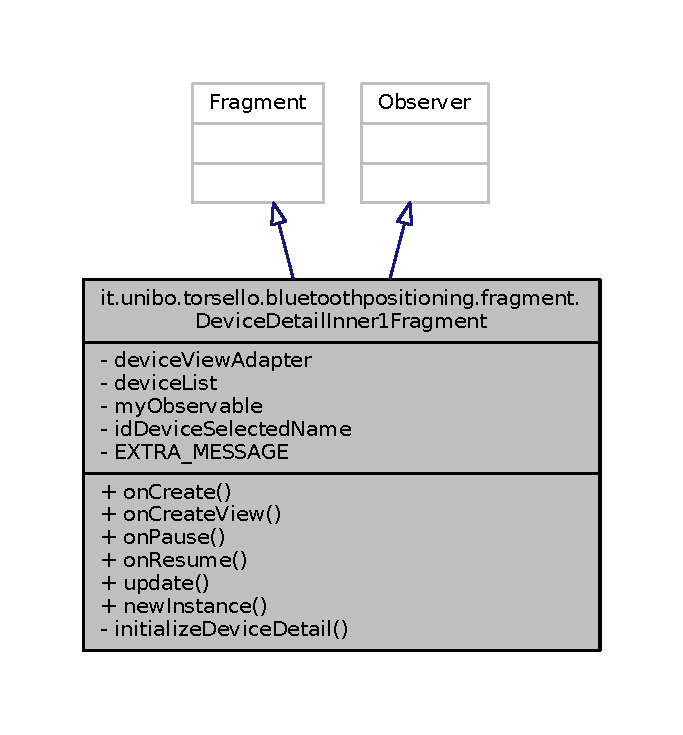
\includegraphics[width=328pt]{classit_1_1unibo_1_1torsello_1_1bluetoothpositioning_1_1fragment_1_1DeviceDetailInner1Fragment__inherit__graph}
\end{center}
\end{figure}


Diagramma di collaborazione per it.\+unibo.\+torsello.\+bluetoothpositioning.\+fragment.\+Device\+Detail\+Inner1\+Fragment\+:
\nopagebreak
\begin{figure}[H]
\begin{center}
\leavevmode
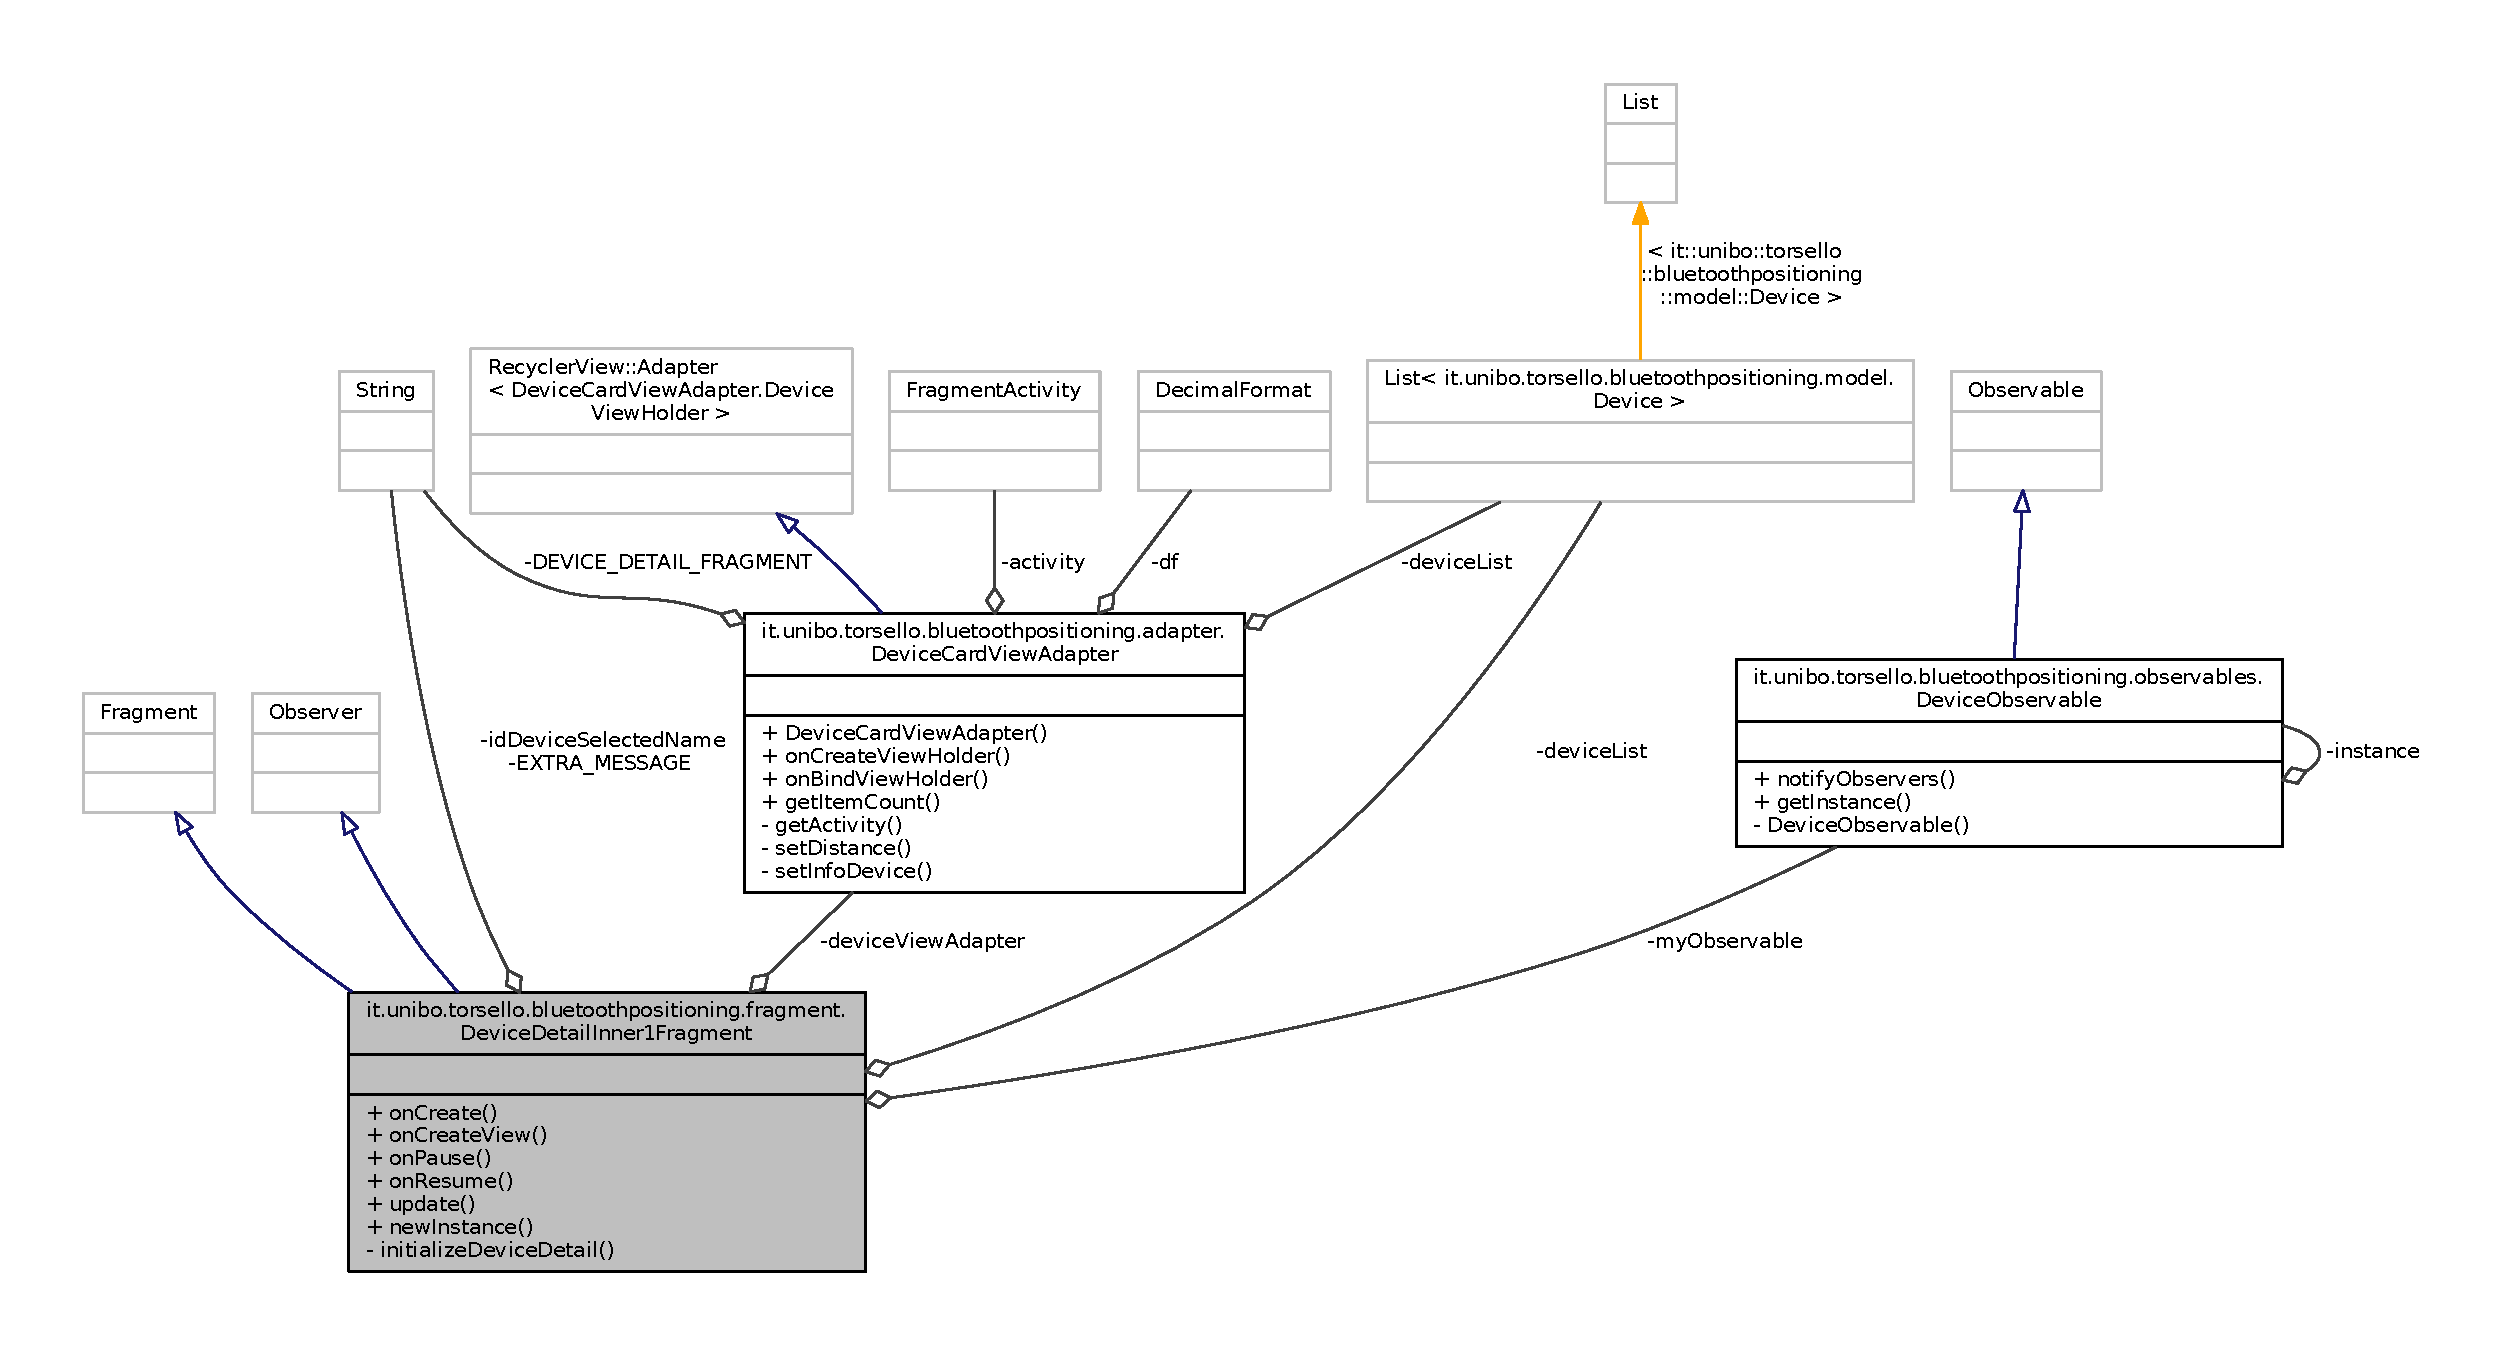
\includegraphics[width=350pt]{classit_1_1unibo_1_1torsello_1_1bluetoothpositioning_1_1fragment_1_1DeviceDetailInner1Fragment__coll__graph}
\end{center}
\end{figure}
\subsubsection*{Membri pubblici}
\begin{DoxyCompactItemize}
\item 
void \hyperlink{classit_1_1unibo_1_1torsello_1_1bluetoothpositioning_1_1fragment_1_1DeviceDetailInner1Fragment_aaa8488de9fd9d2664615301e0f0d15b7_aaa8488de9fd9d2664615301e0f0d15b7}{on\+Create} (@Nullable Bundle saved\+Instance\+State)
\item 
View \hyperlink{classit_1_1unibo_1_1torsello_1_1bluetoothpositioning_1_1fragment_1_1DeviceDetailInner1Fragment_ae5c81b4c40cb3a4d4efda932434bbb7c_ae5c81b4c40cb3a4d4efda932434bbb7c}{on\+Create\+View} (Layout\+Inflater inflater, View\+Group container, Bundle saved\+Instance\+State)
\item 
void \hyperlink{classit_1_1unibo_1_1torsello_1_1bluetoothpositioning_1_1fragment_1_1DeviceDetailInner1Fragment_a7579453e29121da309ed08d902be67b9_a7579453e29121da309ed08d902be67b9}{on\+Pause} ()
\item 
void \hyperlink{classit_1_1unibo_1_1torsello_1_1bluetoothpositioning_1_1fragment_1_1DeviceDetailInner1Fragment_ae54c5f54c5c3fde90927916d41bc284e_ae54c5f54c5c3fde90927916d41bc284e}{on\+Resume} ()
\item 
void \hyperlink{classit_1_1unibo_1_1torsello_1_1bluetoothpositioning_1_1fragment_1_1DeviceDetailInner1Fragment_ad64b7a4bff76d27a4fef8d14760e347b_ad64b7a4bff76d27a4fef8d14760e347b}{update} (Observable o, Object arg)
\end{DoxyCompactItemize}
\subsubsection*{Membri pubblici statici}
\begin{DoxyCompactItemize}
\item 
static \hyperlink{classit_1_1unibo_1_1torsello_1_1bluetoothpositioning_1_1fragment_1_1DeviceDetailInner1Fragment}{Device\+Detail\+Inner1\+Fragment} \hyperlink{classit_1_1unibo_1_1torsello_1_1bluetoothpositioning_1_1fragment_1_1DeviceDetailInner1Fragment_a24fbb536786e1e87e8621b126bd27507_a24fbb536786e1e87e8621b126bd27507}{new\+Instance} (String message)
\end{DoxyCompactItemize}
\subsubsection*{Membri privati}
\begin{DoxyCompactItemize}
\item 
void \hyperlink{classit_1_1unibo_1_1torsello_1_1bluetoothpositioning_1_1fragment_1_1DeviceDetailInner1Fragment_a1d1f9def45a374e0fd22bf443ff609a4_a1d1f9def45a374e0fd22bf443ff609a4}{initialize\+Device\+Detail} (View root)
\end{DoxyCompactItemize}
\subsubsection*{Attributi privati}
\begin{DoxyCompactItemize}
\item 
\hyperlink{classit_1_1unibo_1_1torsello_1_1bluetoothpositioning_1_1adapter_1_1DeviceCardViewAdapter}{Device\+Card\+View\+Adapter} \hyperlink{classit_1_1unibo_1_1torsello_1_1bluetoothpositioning_1_1fragment_1_1DeviceDetailInner1Fragment_ac96cc01fc4f531a4cb38a31cf56e81e9_ac96cc01fc4f531a4cb38a31cf56e81e9}{device\+View\+Adapter}
\item 
List$<$ \hyperlink{classit_1_1unibo_1_1torsello_1_1bluetoothpositioning_1_1model_1_1Device}{Device} $>$ \hyperlink{classit_1_1unibo_1_1torsello_1_1bluetoothpositioning_1_1fragment_1_1DeviceDetailInner1Fragment_a9e1211f228949b78f453eb9a65d93752_a9e1211f228949b78f453eb9a65d93752}{device\+List}
\item 
\hyperlink{classit_1_1unibo_1_1torsello_1_1bluetoothpositioning_1_1observables_1_1DeviceObservable}{Device\+Observable} \hyperlink{classit_1_1unibo_1_1torsello_1_1bluetoothpositioning_1_1fragment_1_1DeviceDetailInner1Fragment_a237134f174fd95371d0a7725b9a81183_a237134f174fd95371d0a7725b9a81183}{my\+Observable}
\item 
String \hyperlink{classit_1_1unibo_1_1torsello_1_1bluetoothpositioning_1_1fragment_1_1DeviceDetailInner1Fragment_a15c5b5dd3b89ff572fb25b5825ef6fdf_a15c5b5dd3b89ff572fb25b5825ef6fdf}{id\+Device\+Selected\+Name}
\end{DoxyCompactItemize}
\subsubsection*{Attributi privati statici}
\begin{DoxyCompactItemize}
\item 
static final String \hyperlink{classit_1_1unibo_1_1torsello_1_1bluetoothpositioning_1_1fragment_1_1DeviceDetailInner1Fragment_ac0b0104608454a0d84a47ad82ef186fc_ac0b0104608454a0d84a47ad82ef186fc}{E\+X\+T\+R\+A\+\_\+\+M\+E\+S\+S\+A\+GE} = \char`\"{}E\+X\+T\+R\+A\+\_\+\+M\+E\+S\+S\+A\+GE\char`\"{}
\end{DoxyCompactItemize}


\subsubsection{Descrizione dettagliata}
Created by Federico Torsello. \href{mailto:federico.torsello@studio.unibo.it}{\tt federico.\+torsello@studio.\+unibo.\+it} 

\subsubsection{Documentazione delle funzioni membro}
\hypertarget{classit_1_1unibo_1_1torsello_1_1bluetoothpositioning_1_1fragment_1_1DeviceDetailInner1Fragment_a1d1f9def45a374e0fd22bf443ff609a4_a1d1f9def45a374e0fd22bf443ff609a4}{}\label{classit_1_1unibo_1_1torsello_1_1bluetoothpositioning_1_1fragment_1_1DeviceDetailInner1Fragment_a1d1f9def45a374e0fd22bf443ff609a4_a1d1f9def45a374e0fd22bf443ff609a4} 
\index{it\+::unibo\+::torsello\+::bluetoothpositioning\+::fragment\+::\+Device\+Detail\+Inner1\+Fragment@{it\+::unibo\+::torsello\+::bluetoothpositioning\+::fragment\+::\+Device\+Detail\+Inner1\+Fragment}!initialize\+Device\+Detail@{initialize\+Device\+Detail}}
\index{initialize\+Device\+Detail@{initialize\+Device\+Detail}!it\+::unibo\+::torsello\+::bluetoothpositioning\+::fragment\+::\+Device\+Detail\+Inner1\+Fragment@{it\+::unibo\+::torsello\+::bluetoothpositioning\+::fragment\+::\+Device\+Detail\+Inner1\+Fragment}}
\paragraph{\texorpdfstring{initialize\+Device\+Detail()}{initializeDeviceDetail()}}
{\footnotesize\ttfamily void it.\+unibo.\+torsello.\+bluetoothpositioning.\+fragment.\+Device\+Detail\+Inner1\+Fragment.\+initialize\+Device\+Detail (\begin{DoxyParamCaption}\item[{View}]{root }\end{DoxyParamCaption})\hspace{0.3cm}{\ttfamily [private]}}


\begin{DoxyCode}
75                                                    \{
76         \textcolor{comment}{// add RecyclerView}
77         RecyclerView recyclerView = (RecyclerView) root.findViewById(R.id.recycler\_view\_detail);
78         recyclerView.setLayoutManager(\textcolor{keyword}{new} LinearLayoutManager(getContext()));
79         recyclerView.setAdapter(\hyperlink{classit_1_1unibo_1_1torsello_1_1bluetoothpositioning_1_1fragment_1_1DeviceDetailInner1Fragment_ac96cc01fc4f531a4cb38a31cf56e81e9_ac96cc01fc4f531a4cb38a31cf56e81e9}{deviceViewAdapter});
80     \}
\end{DoxyCode}
\hypertarget{classit_1_1unibo_1_1torsello_1_1bluetoothpositioning_1_1fragment_1_1DeviceDetailInner1Fragment_a24fbb536786e1e87e8621b126bd27507_a24fbb536786e1e87e8621b126bd27507}{}\label{classit_1_1unibo_1_1torsello_1_1bluetoothpositioning_1_1fragment_1_1DeviceDetailInner1Fragment_a24fbb536786e1e87e8621b126bd27507_a24fbb536786e1e87e8621b126bd27507} 
\index{it\+::unibo\+::torsello\+::bluetoothpositioning\+::fragment\+::\+Device\+Detail\+Inner1\+Fragment@{it\+::unibo\+::torsello\+::bluetoothpositioning\+::fragment\+::\+Device\+Detail\+Inner1\+Fragment}!new\+Instance@{new\+Instance}}
\index{new\+Instance@{new\+Instance}!it\+::unibo\+::torsello\+::bluetoothpositioning\+::fragment\+::\+Device\+Detail\+Inner1\+Fragment@{it\+::unibo\+::torsello\+::bluetoothpositioning\+::fragment\+::\+Device\+Detail\+Inner1\+Fragment}}
\paragraph{\texorpdfstring{new\+Instance()}{newInstance()}}
{\footnotesize\ttfamily static \hyperlink{classit_1_1unibo_1_1torsello_1_1bluetoothpositioning_1_1fragment_1_1DeviceDetailInner1Fragment}{Device\+Detail\+Inner1\+Fragment} it.\+unibo.\+torsello.\+bluetoothpositioning.\+fragment.\+Device\+Detail\+Inner1\+Fragment.\+new\+Instance (\begin{DoxyParamCaption}\item[{String}]{message }\end{DoxyParamCaption})\hspace{0.3cm}{\ttfamily [static]}}


\begin{DoxyCode}
35                                                                          \{
36         DeviceDetailInner1Fragment fragment = \textcolor{keyword}{new} DeviceDetailInner1Fragment();
37         Bundle args = \textcolor{keyword}{new} Bundle();
38         args.putString(\hyperlink{classit_1_1unibo_1_1torsello_1_1bluetoothpositioning_1_1fragment_1_1DeviceDetailInner1Fragment_ac0b0104608454a0d84a47ad82ef186fc_ac0b0104608454a0d84a47ad82ef186fc}{EXTRA\_MESSAGE}, message);
39         fragment.setArguments(args);
40         \textcolor{keywordflow}{return} fragment;
41     \}
\end{DoxyCode}
\hypertarget{classit_1_1unibo_1_1torsello_1_1bluetoothpositioning_1_1fragment_1_1DeviceDetailInner1Fragment_aaa8488de9fd9d2664615301e0f0d15b7_aaa8488de9fd9d2664615301e0f0d15b7}{}\label{classit_1_1unibo_1_1torsello_1_1bluetoothpositioning_1_1fragment_1_1DeviceDetailInner1Fragment_aaa8488de9fd9d2664615301e0f0d15b7_aaa8488de9fd9d2664615301e0f0d15b7} 
\index{it\+::unibo\+::torsello\+::bluetoothpositioning\+::fragment\+::\+Device\+Detail\+Inner1\+Fragment@{it\+::unibo\+::torsello\+::bluetoothpositioning\+::fragment\+::\+Device\+Detail\+Inner1\+Fragment}!on\+Create@{on\+Create}}
\index{on\+Create@{on\+Create}!it\+::unibo\+::torsello\+::bluetoothpositioning\+::fragment\+::\+Device\+Detail\+Inner1\+Fragment@{it\+::unibo\+::torsello\+::bluetoothpositioning\+::fragment\+::\+Device\+Detail\+Inner1\+Fragment}}
\paragraph{\texorpdfstring{on\+Create()}{onCreate()}}
{\footnotesize\ttfamily void it.\+unibo.\+torsello.\+bluetoothpositioning.\+fragment.\+Device\+Detail\+Inner1\+Fragment.\+on\+Create (\begin{DoxyParamCaption}\item[{@Nullable Bundle}]{saved\+Instance\+State }\end{DoxyParamCaption})}


\begin{DoxyCode}
44                                                               \{
45         super.onCreate(savedInstanceState);
46 
47         \hyperlink{classit_1_1unibo_1_1torsello_1_1bluetoothpositioning_1_1fragment_1_1DeviceDetailInner1Fragment_a237134f174fd95371d0a7725b9a81183_a237134f174fd95371d0a7725b9a81183}{myObservable} = DeviceObservable.\hyperlink{classit_1_1unibo_1_1torsello_1_1bluetoothpositioning_1_1observables_1_1DeviceObservable_ab16792c5848440646624b2a41553954a_ab16792c5848440646624b2a41553954a}{getInstance}();
48 
49         \hyperlink{classit_1_1unibo_1_1torsello_1_1bluetoothpositioning_1_1fragment_1_1DeviceDetailInner1Fragment_a15c5b5dd3b89ff572fb25b5825ef6fdf_a15c5b5dd3b89ff572fb25b5825ef6fdf}{idDeviceSelectedName} = getArguments().getString(
      \hyperlink{classit_1_1unibo_1_1torsello_1_1bluetoothpositioning_1_1fragment_1_1DeviceDetailInner1Fragment_ac0b0104608454a0d84a47ad82ef186fc_ac0b0104608454a0d84a47ad82ef186fc}{EXTRA\_MESSAGE});
50         \hyperlink{classit_1_1unibo_1_1torsello_1_1bluetoothpositioning_1_1fragment_1_1DeviceDetailInner1Fragment_a9e1211f228949b78f453eb9a65d93752_a9e1211f228949b78f453eb9a65d93752}{deviceList} = \textcolor{keyword}{new} ArrayList<>();
51         \hyperlink{classit_1_1unibo_1_1torsello_1_1bluetoothpositioning_1_1fragment_1_1DeviceDetailInner1Fragment_ac96cc01fc4f531a4cb38a31cf56e81e9_ac96cc01fc4f531a4cb38a31cf56e81e9}{deviceViewAdapter} = \textcolor{keyword}{new} DeviceCardViewAdapter(getActivity(), 
      \hyperlink{classit_1_1unibo_1_1torsello_1_1bluetoothpositioning_1_1fragment_1_1DeviceDetailInner1Fragment_a9e1211f228949b78f453eb9a65d93752_a9e1211f228949b78f453eb9a65d93752}{deviceList});
52     \}
\end{DoxyCode}
\hypertarget{classit_1_1unibo_1_1torsello_1_1bluetoothpositioning_1_1fragment_1_1DeviceDetailInner1Fragment_ae5c81b4c40cb3a4d4efda932434bbb7c_ae5c81b4c40cb3a4d4efda932434bbb7c}{}\label{classit_1_1unibo_1_1torsello_1_1bluetoothpositioning_1_1fragment_1_1DeviceDetailInner1Fragment_ae5c81b4c40cb3a4d4efda932434bbb7c_ae5c81b4c40cb3a4d4efda932434bbb7c} 
\index{it\+::unibo\+::torsello\+::bluetoothpositioning\+::fragment\+::\+Device\+Detail\+Inner1\+Fragment@{it\+::unibo\+::torsello\+::bluetoothpositioning\+::fragment\+::\+Device\+Detail\+Inner1\+Fragment}!on\+Create\+View@{on\+Create\+View}}
\index{on\+Create\+View@{on\+Create\+View}!it\+::unibo\+::torsello\+::bluetoothpositioning\+::fragment\+::\+Device\+Detail\+Inner1\+Fragment@{it\+::unibo\+::torsello\+::bluetoothpositioning\+::fragment\+::\+Device\+Detail\+Inner1\+Fragment}}
\paragraph{\texorpdfstring{on\+Create\+View()}{onCreateView()}}
{\footnotesize\ttfamily View it.\+unibo.\+torsello.\+bluetoothpositioning.\+fragment.\+Device\+Detail\+Inner1\+Fragment.\+on\+Create\+View (\begin{DoxyParamCaption}\item[{Layout\+Inflater}]{inflater,  }\item[{View\+Group}]{container,  }\item[{Bundle}]{saved\+Instance\+State }\end{DoxyParamCaption})}


\begin{DoxyCode}
55                                                                                                       \{
56         View root = inflater.inflate(R.layout.fragment\_device\_detail\_inner\_1, container, \textcolor{keyword}{false});
57 
58         \hyperlink{classit_1_1unibo_1_1torsello_1_1bluetoothpositioning_1_1fragment_1_1DeviceDetailInner1Fragment_a1d1f9def45a374e0fd22bf443ff609a4_a1d1f9def45a374e0fd22bf443ff609a4}{initializeDeviceDetail}(root);
59 
60         \textcolor{keywordflow}{return} root;
61     \}
\end{DoxyCode}
\hypertarget{classit_1_1unibo_1_1torsello_1_1bluetoothpositioning_1_1fragment_1_1DeviceDetailInner1Fragment_a7579453e29121da309ed08d902be67b9_a7579453e29121da309ed08d902be67b9}{}\label{classit_1_1unibo_1_1torsello_1_1bluetoothpositioning_1_1fragment_1_1DeviceDetailInner1Fragment_a7579453e29121da309ed08d902be67b9_a7579453e29121da309ed08d902be67b9} 
\index{it\+::unibo\+::torsello\+::bluetoothpositioning\+::fragment\+::\+Device\+Detail\+Inner1\+Fragment@{it\+::unibo\+::torsello\+::bluetoothpositioning\+::fragment\+::\+Device\+Detail\+Inner1\+Fragment}!on\+Pause@{on\+Pause}}
\index{on\+Pause@{on\+Pause}!it\+::unibo\+::torsello\+::bluetoothpositioning\+::fragment\+::\+Device\+Detail\+Inner1\+Fragment@{it\+::unibo\+::torsello\+::bluetoothpositioning\+::fragment\+::\+Device\+Detail\+Inner1\+Fragment}}
\paragraph{\texorpdfstring{on\+Pause()}{onPause()}}
{\footnotesize\ttfamily void it.\+unibo.\+torsello.\+bluetoothpositioning.\+fragment.\+Device\+Detail\+Inner1\+Fragment.\+on\+Pause (\begin{DoxyParamCaption}{ }\end{DoxyParamCaption})}


\begin{DoxyCode}
64                           \{
65         \hyperlink{classit_1_1unibo_1_1torsello_1_1bluetoothpositioning_1_1fragment_1_1DeviceDetailInner1Fragment_a237134f174fd95371d0a7725b9a81183_a237134f174fd95371d0a7725b9a81183}{myObservable}.deleteObserver(\textcolor{keyword}{this});
66         super.onPause();
67     \}
\end{DoxyCode}
\hypertarget{classit_1_1unibo_1_1torsello_1_1bluetoothpositioning_1_1fragment_1_1DeviceDetailInner1Fragment_ae54c5f54c5c3fde90927916d41bc284e_ae54c5f54c5c3fde90927916d41bc284e}{}\label{classit_1_1unibo_1_1torsello_1_1bluetoothpositioning_1_1fragment_1_1DeviceDetailInner1Fragment_ae54c5f54c5c3fde90927916d41bc284e_ae54c5f54c5c3fde90927916d41bc284e} 
\index{it\+::unibo\+::torsello\+::bluetoothpositioning\+::fragment\+::\+Device\+Detail\+Inner1\+Fragment@{it\+::unibo\+::torsello\+::bluetoothpositioning\+::fragment\+::\+Device\+Detail\+Inner1\+Fragment}!on\+Resume@{on\+Resume}}
\index{on\+Resume@{on\+Resume}!it\+::unibo\+::torsello\+::bluetoothpositioning\+::fragment\+::\+Device\+Detail\+Inner1\+Fragment@{it\+::unibo\+::torsello\+::bluetoothpositioning\+::fragment\+::\+Device\+Detail\+Inner1\+Fragment}}
\paragraph{\texorpdfstring{on\+Resume()}{onResume()}}
{\footnotesize\ttfamily void it.\+unibo.\+torsello.\+bluetoothpositioning.\+fragment.\+Device\+Detail\+Inner1\+Fragment.\+on\+Resume (\begin{DoxyParamCaption}{ }\end{DoxyParamCaption})}


\begin{DoxyCode}
70                            \{
71         super.onResume();
72         \hyperlink{classit_1_1unibo_1_1torsello_1_1bluetoothpositioning_1_1fragment_1_1DeviceDetailInner1Fragment_a237134f174fd95371d0a7725b9a81183_a237134f174fd95371d0a7725b9a81183}{myObservable}.addObserver(\textcolor{keyword}{this});
73     \}
\end{DoxyCode}
\hypertarget{classit_1_1unibo_1_1torsello_1_1bluetoothpositioning_1_1fragment_1_1DeviceDetailInner1Fragment_ad64b7a4bff76d27a4fef8d14760e347b_ad64b7a4bff76d27a4fef8d14760e347b}{}\label{classit_1_1unibo_1_1torsello_1_1bluetoothpositioning_1_1fragment_1_1DeviceDetailInner1Fragment_ad64b7a4bff76d27a4fef8d14760e347b_ad64b7a4bff76d27a4fef8d14760e347b} 
\index{it\+::unibo\+::torsello\+::bluetoothpositioning\+::fragment\+::\+Device\+Detail\+Inner1\+Fragment@{it\+::unibo\+::torsello\+::bluetoothpositioning\+::fragment\+::\+Device\+Detail\+Inner1\+Fragment}!update@{update}}
\index{update@{update}!it\+::unibo\+::torsello\+::bluetoothpositioning\+::fragment\+::\+Device\+Detail\+Inner1\+Fragment@{it\+::unibo\+::torsello\+::bluetoothpositioning\+::fragment\+::\+Device\+Detail\+Inner1\+Fragment}}
\paragraph{\texorpdfstring{update()}{update()}}
{\footnotesize\ttfamily void it.\+unibo.\+torsello.\+bluetoothpositioning.\+fragment.\+Device\+Detail\+Inner1\+Fragment.\+update (\begin{DoxyParamCaption}\item[{Observable}]{o,  }\item[{Object}]{arg }\end{DoxyParamCaption})}


\begin{DoxyCode}
83                                                  \{
84 
85         \textcolor{keywordflow}{if} (arg instanceof List) \{
86 
87             \textcolor{keywordflow}{if} (!\hyperlink{classit_1_1unibo_1_1torsello_1_1bluetoothpositioning_1_1fragment_1_1DeviceDetailInner1Fragment_a9e1211f228949b78f453eb9a65d93752_a9e1211f228949b78f453eb9a65d93752}{deviceList}.isEmpty()) \{
88                 \hyperlink{classit_1_1unibo_1_1torsello_1_1bluetoothpositioning_1_1fragment_1_1DeviceDetailInner1Fragment_a9e1211f228949b78f453eb9a65d93752_a9e1211f228949b78f453eb9a65d93752}{deviceList}.clear();
89             \}
90 
91             List<Device> devices = (List<Device>) arg;
92 
93             \textcolor{keywordflow}{for} (Device deviceSelected : devices) \{
94                 \textcolor{keywordflow}{if} (deviceSelected.getFriendlyName().equals(\hyperlink{classit_1_1unibo_1_1torsello_1_1bluetoothpositioning_1_1fragment_1_1DeviceDetailInner1Fragment_a15c5b5dd3b89ff572fb25b5825ef6fdf_a15c5b5dd3b89ff572fb25b5825ef6fdf}{idDeviceSelectedName}) ||
95                         deviceSelected.getAddress().equals(\hyperlink{classit_1_1unibo_1_1torsello_1_1bluetoothpositioning_1_1fragment_1_1DeviceDetailInner1Fragment_a15c5b5dd3b89ff572fb25b5825ef6fdf_a15c5b5dd3b89ff572fb25b5825ef6fdf}{idDeviceSelectedName})) \{
96                     \hyperlink{classit_1_1unibo_1_1torsello_1_1bluetoothpositioning_1_1fragment_1_1DeviceDetailInner1Fragment_a9e1211f228949b78f453eb9a65d93752_a9e1211f228949b78f453eb9a65d93752}{deviceList}.add(deviceSelected);
97                 \}
98             \}
99 
100             \hyperlink{classit_1_1unibo_1_1torsello_1_1bluetoothpositioning_1_1fragment_1_1DeviceDetailInner1Fragment_ac96cc01fc4f531a4cb38a31cf56e81e9_ac96cc01fc4f531a4cb38a31cf56e81e9}{deviceViewAdapter}.notifyDataSetChanged();
101         \}
102     \}
\end{DoxyCode}


\subsubsection{Documentazione dei membri dato}
\hypertarget{classit_1_1unibo_1_1torsello_1_1bluetoothpositioning_1_1fragment_1_1DeviceDetailInner1Fragment_a9e1211f228949b78f453eb9a65d93752_a9e1211f228949b78f453eb9a65d93752}{}\label{classit_1_1unibo_1_1torsello_1_1bluetoothpositioning_1_1fragment_1_1DeviceDetailInner1Fragment_a9e1211f228949b78f453eb9a65d93752_a9e1211f228949b78f453eb9a65d93752} 
\index{it\+::unibo\+::torsello\+::bluetoothpositioning\+::fragment\+::\+Device\+Detail\+Inner1\+Fragment@{it\+::unibo\+::torsello\+::bluetoothpositioning\+::fragment\+::\+Device\+Detail\+Inner1\+Fragment}!device\+List@{device\+List}}
\index{device\+List@{device\+List}!it\+::unibo\+::torsello\+::bluetoothpositioning\+::fragment\+::\+Device\+Detail\+Inner1\+Fragment@{it\+::unibo\+::torsello\+::bluetoothpositioning\+::fragment\+::\+Device\+Detail\+Inner1\+Fragment}}
\paragraph{\texorpdfstring{device\+List}{deviceList}}
{\footnotesize\ttfamily List$<$\hyperlink{classit_1_1unibo_1_1torsello_1_1bluetoothpositioning_1_1model_1_1Device}{Device}$>$ it.\+unibo.\+torsello.\+bluetoothpositioning.\+fragment.\+Device\+Detail\+Inner1\+Fragment.\+device\+List\hspace{0.3cm}{\ttfamily [private]}}

\hypertarget{classit_1_1unibo_1_1torsello_1_1bluetoothpositioning_1_1fragment_1_1DeviceDetailInner1Fragment_ac96cc01fc4f531a4cb38a31cf56e81e9_ac96cc01fc4f531a4cb38a31cf56e81e9}{}\label{classit_1_1unibo_1_1torsello_1_1bluetoothpositioning_1_1fragment_1_1DeviceDetailInner1Fragment_ac96cc01fc4f531a4cb38a31cf56e81e9_ac96cc01fc4f531a4cb38a31cf56e81e9} 
\index{it\+::unibo\+::torsello\+::bluetoothpositioning\+::fragment\+::\+Device\+Detail\+Inner1\+Fragment@{it\+::unibo\+::torsello\+::bluetoothpositioning\+::fragment\+::\+Device\+Detail\+Inner1\+Fragment}!device\+View\+Adapter@{device\+View\+Adapter}}
\index{device\+View\+Adapter@{device\+View\+Adapter}!it\+::unibo\+::torsello\+::bluetoothpositioning\+::fragment\+::\+Device\+Detail\+Inner1\+Fragment@{it\+::unibo\+::torsello\+::bluetoothpositioning\+::fragment\+::\+Device\+Detail\+Inner1\+Fragment}}
\paragraph{\texorpdfstring{device\+View\+Adapter}{deviceViewAdapter}}
{\footnotesize\ttfamily \hyperlink{classit_1_1unibo_1_1torsello_1_1bluetoothpositioning_1_1adapter_1_1DeviceCardViewAdapter}{Device\+Card\+View\+Adapter} it.\+unibo.\+torsello.\+bluetoothpositioning.\+fragment.\+Device\+Detail\+Inner1\+Fragment.\+device\+View\+Adapter\hspace{0.3cm}{\ttfamily [private]}}

\hypertarget{classit_1_1unibo_1_1torsello_1_1bluetoothpositioning_1_1fragment_1_1DeviceDetailInner1Fragment_ac0b0104608454a0d84a47ad82ef186fc_ac0b0104608454a0d84a47ad82ef186fc}{}\label{classit_1_1unibo_1_1torsello_1_1bluetoothpositioning_1_1fragment_1_1DeviceDetailInner1Fragment_ac0b0104608454a0d84a47ad82ef186fc_ac0b0104608454a0d84a47ad82ef186fc} 
\index{it\+::unibo\+::torsello\+::bluetoothpositioning\+::fragment\+::\+Device\+Detail\+Inner1\+Fragment@{it\+::unibo\+::torsello\+::bluetoothpositioning\+::fragment\+::\+Device\+Detail\+Inner1\+Fragment}!E\+X\+T\+R\+A\+\_\+\+M\+E\+S\+S\+A\+GE@{E\+X\+T\+R\+A\+\_\+\+M\+E\+S\+S\+A\+GE}}
\index{E\+X\+T\+R\+A\+\_\+\+M\+E\+S\+S\+A\+GE@{E\+X\+T\+R\+A\+\_\+\+M\+E\+S\+S\+A\+GE}!it\+::unibo\+::torsello\+::bluetoothpositioning\+::fragment\+::\+Device\+Detail\+Inner1\+Fragment@{it\+::unibo\+::torsello\+::bluetoothpositioning\+::fragment\+::\+Device\+Detail\+Inner1\+Fragment}}
\paragraph{\texorpdfstring{E\+X\+T\+R\+A\+\_\+\+M\+E\+S\+S\+A\+GE}{EXTRA\_MESSAGE}}
{\footnotesize\ttfamily final String it.\+unibo.\+torsello.\+bluetoothpositioning.\+fragment.\+Device\+Detail\+Inner1\+Fragment.\+E\+X\+T\+R\+A\+\_\+\+M\+E\+S\+S\+A\+GE = \char`\"{}E\+X\+T\+R\+A\+\_\+\+M\+E\+S\+S\+A\+GE\char`\"{}\hspace{0.3cm}{\ttfamily [static]}, {\ttfamily [private]}}

\hypertarget{classit_1_1unibo_1_1torsello_1_1bluetoothpositioning_1_1fragment_1_1DeviceDetailInner1Fragment_a15c5b5dd3b89ff572fb25b5825ef6fdf_a15c5b5dd3b89ff572fb25b5825ef6fdf}{}\label{classit_1_1unibo_1_1torsello_1_1bluetoothpositioning_1_1fragment_1_1DeviceDetailInner1Fragment_a15c5b5dd3b89ff572fb25b5825ef6fdf_a15c5b5dd3b89ff572fb25b5825ef6fdf} 
\index{it\+::unibo\+::torsello\+::bluetoothpositioning\+::fragment\+::\+Device\+Detail\+Inner1\+Fragment@{it\+::unibo\+::torsello\+::bluetoothpositioning\+::fragment\+::\+Device\+Detail\+Inner1\+Fragment}!id\+Device\+Selected\+Name@{id\+Device\+Selected\+Name}}
\index{id\+Device\+Selected\+Name@{id\+Device\+Selected\+Name}!it\+::unibo\+::torsello\+::bluetoothpositioning\+::fragment\+::\+Device\+Detail\+Inner1\+Fragment@{it\+::unibo\+::torsello\+::bluetoothpositioning\+::fragment\+::\+Device\+Detail\+Inner1\+Fragment}}
\paragraph{\texorpdfstring{id\+Device\+Selected\+Name}{idDeviceSelectedName}}
{\footnotesize\ttfamily String it.\+unibo.\+torsello.\+bluetoothpositioning.\+fragment.\+Device\+Detail\+Inner1\+Fragment.\+id\+Device\+Selected\+Name\hspace{0.3cm}{\ttfamily [private]}}

\hypertarget{classit_1_1unibo_1_1torsello_1_1bluetoothpositioning_1_1fragment_1_1DeviceDetailInner1Fragment_a237134f174fd95371d0a7725b9a81183_a237134f174fd95371d0a7725b9a81183}{}\label{classit_1_1unibo_1_1torsello_1_1bluetoothpositioning_1_1fragment_1_1DeviceDetailInner1Fragment_a237134f174fd95371d0a7725b9a81183_a237134f174fd95371d0a7725b9a81183} 
\index{it\+::unibo\+::torsello\+::bluetoothpositioning\+::fragment\+::\+Device\+Detail\+Inner1\+Fragment@{it\+::unibo\+::torsello\+::bluetoothpositioning\+::fragment\+::\+Device\+Detail\+Inner1\+Fragment}!my\+Observable@{my\+Observable}}
\index{my\+Observable@{my\+Observable}!it\+::unibo\+::torsello\+::bluetoothpositioning\+::fragment\+::\+Device\+Detail\+Inner1\+Fragment@{it\+::unibo\+::torsello\+::bluetoothpositioning\+::fragment\+::\+Device\+Detail\+Inner1\+Fragment}}
\paragraph{\texorpdfstring{my\+Observable}{myObservable}}
{\footnotesize\ttfamily \hyperlink{classit_1_1unibo_1_1torsello_1_1bluetoothpositioning_1_1observables_1_1DeviceObservable}{Device\+Observable} it.\+unibo.\+torsello.\+bluetoothpositioning.\+fragment.\+Device\+Detail\+Inner1\+Fragment.\+my\+Observable\hspace{0.3cm}{\ttfamily [private]}}



La documentazione per questa classe è stata generata a partire dal seguente file\+:\begin{DoxyCompactItemize}
\item 
\hyperlink{DeviceDetailInner1Fragment_8java}{Device\+Detail\+Inner1\+Fragment.\+java}\end{DoxyCompactItemize}

\hypertarget{classit_1_1unibo_1_1torsello_1_1bluetoothpositioning_1_1fragment_1_1DeviceDetailInner2Fragment}{}\subsection{Riferimenti per la classe it.\+unibo.\+torsello.\+bluetoothpositioning.\+fragment.\+Device\+Detail\+Inner2\+Fragment}
\label{classit_1_1unibo_1_1torsello_1_1bluetoothpositioning_1_1fragment_1_1DeviceDetailInner2Fragment}\index{it.\+unibo.\+torsello.\+bluetoothpositioning.\+fragment.\+Device\+Detail\+Inner2\+Fragment@{it.\+unibo.\+torsello.\+bluetoothpositioning.\+fragment.\+Device\+Detail\+Inner2\+Fragment}}


Diagramma delle classi per it.\+unibo.\+torsello.\+bluetoothpositioning.\+fragment.\+Device\+Detail\+Inner2\+Fragment
\nopagebreak
\begin{figure}[H]
\begin{center}
\leavevmode
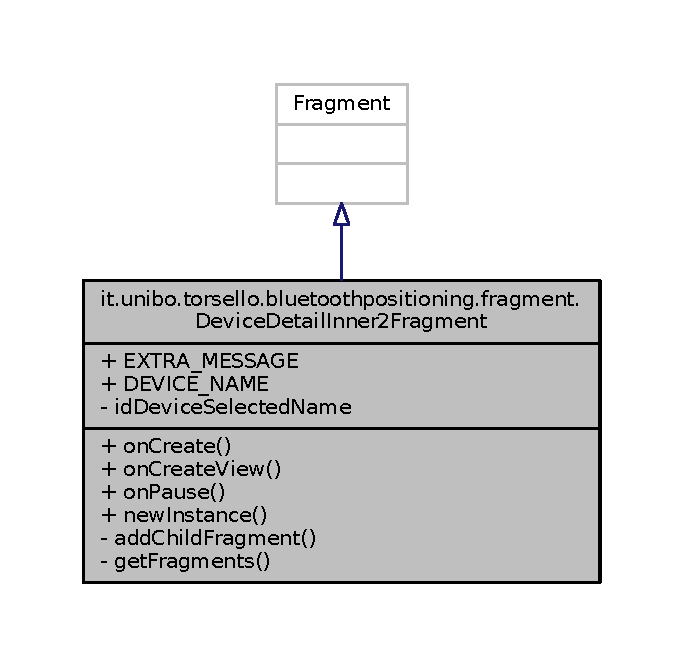
\includegraphics[width=328pt]{classit_1_1unibo_1_1torsello_1_1bluetoothpositioning_1_1fragment_1_1DeviceDetailInner2Fragment__inherit__graph}
\end{center}
\end{figure}


Diagramma di collaborazione per it.\+unibo.\+torsello.\+bluetoothpositioning.\+fragment.\+Device\+Detail\+Inner2\+Fragment\+:
\nopagebreak
\begin{figure}[H]
\begin{center}
\leavevmode
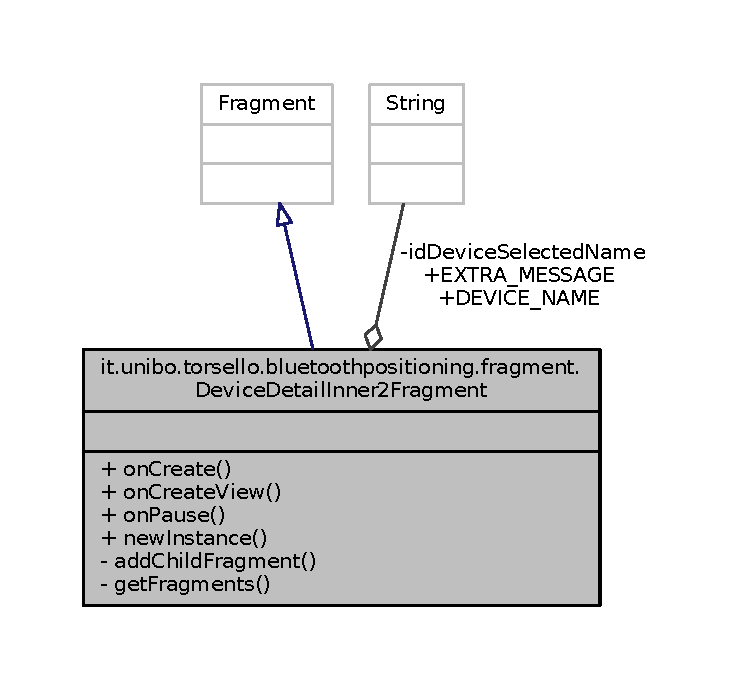
\includegraphics[width=350pt]{classit_1_1unibo_1_1torsello_1_1bluetoothpositioning_1_1fragment_1_1DeviceDetailInner2Fragment__coll__graph}
\end{center}
\end{figure}
\subsubsection*{Membri pubblici}
\begin{DoxyCompactItemize}
\item 
void \hyperlink{classit_1_1unibo_1_1torsello_1_1bluetoothpositioning_1_1fragment_1_1DeviceDetailInner2Fragment_a0f0b6b90d40bb3f44a66de91da787f75_a0f0b6b90d40bb3f44a66de91da787f75}{on\+Create} (Bundle saved\+Instance\+State)
\item 
View \hyperlink{classit_1_1unibo_1_1torsello_1_1bluetoothpositioning_1_1fragment_1_1DeviceDetailInner2Fragment_aaaab1478726f0d8a4b9bdfe3eab122c8_aaaab1478726f0d8a4b9bdfe3eab122c8}{on\+Create\+View} (Layout\+Inflater inflater, View\+Group container, Bundle saved\+Instance\+State)
\item 
void \hyperlink{classit_1_1unibo_1_1torsello_1_1bluetoothpositioning_1_1fragment_1_1DeviceDetailInner2Fragment_ab201a51f09d4ccd17f91d5952b9ed788_ab201a51f09d4ccd17f91d5952b9ed788}{on\+Pause} ()
\end{DoxyCompactItemize}
\subsubsection*{Membri pubblici statici}
\begin{DoxyCompactItemize}
\item 
static \hyperlink{classit_1_1unibo_1_1torsello_1_1bluetoothpositioning_1_1fragment_1_1DeviceDetailInner2Fragment}{Device\+Detail\+Inner2\+Fragment} \hyperlink{classit_1_1unibo_1_1torsello_1_1bluetoothpositioning_1_1fragment_1_1DeviceDetailInner2Fragment_a27471a2d140a8dd11636ef23ffc20657_a27471a2d140a8dd11636ef23ffc20657}{new\+Instance} (String message, String device\+Name)
\end{DoxyCompactItemize}
\subsubsection*{Membri privati}
\begin{DoxyCompactItemize}
\item 
void \hyperlink{classit_1_1unibo_1_1torsello_1_1bluetoothpositioning_1_1fragment_1_1DeviceDetailInner2Fragment_af61900b6821dff2086e86d646c990870_af61900b6821dff2086e86d646c990870}{add\+Child\+Fragment} (View root)
\item 
Array\+List$<$ Fragment $>$ \hyperlink{classit_1_1unibo_1_1torsello_1_1bluetoothpositioning_1_1fragment_1_1DeviceDetailInner2Fragment_a74ebcb936381919cfe4f3542585203c4_a74ebcb936381919cfe4f3542585203c4}{get\+Fragments} ()
\end{DoxyCompactItemize}
\subsubsection*{Attributi privati}
\begin{DoxyCompactItemize}
\item 
String \hyperlink{classit_1_1unibo_1_1torsello_1_1bluetoothpositioning_1_1fragment_1_1DeviceDetailInner2Fragment_a84cd6ba00a3c2e8b7a53cac62c73f1b5_a84cd6ba00a3c2e8b7a53cac62c73f1b5}{id\+Device\+Selected\+Name}
\end{DoxyCompactItemize}
\subsubsection*{Attributi privati statici}
\begin{DoxyCompactItemize}
\item 
static final String \hyperlink{classit_1_1unibo_1_1torsello_1_1bluetoothpositioning_1_1fragment_1_1DeviceDetailInner2Fragment_a5093b051b0d458a870b6eef51b088e7d_a5093b051b0d458a870b6eef51b088e7d}{E\+X\+T\+R\+A\+\_\+\+M\+E\+S\+S\+A\+GE} = \char`\"{}E\+X\+T\+R\+A\+\_\+\+M\+E\+S\+S\+A\+GE\char`\"{}
\item 
static final String \hyperlink{classit_1_1unibo_1_1torsello_1_1bluetoothpositioning_1_1fragment_1_1DeviceDetailInner2Fragment_aa28d537983d4cf578120a9c51eb2b0bb_aa28d537983d4cf578120a9c51eb2b0bb}{D\+E\+V\+I\+C\+E\+\_\+\+N\+A\+ME} = \char`\"{}D\+E\+V\+I\+C\+E\+\_\+\+N\+A\+ME\char`\"{}
\end{DoxyCompactItemize}


\subsubsection{Descrizione dettagliata}
Created by Federico Torsello. \href{mailto:federico.torsello@studio.unibo.it}{\tt federico.\+torsello@studio.\+unibo.\+it} 

\subsubsection{Documentazione delle funzioni membro}
\hypertarget{classit_1_1unibo_1_1torsello_1_1bluetoothpositioning_1_1fragment_1_1DeviceDetailInner2Fragment_af61900b6821dff2086e86d646c990870_af61900b6821dff2086e86d646c990870}{}\label{classit_1_1unibo_1_1torsello_1_1bluetoothpositioning_1_1fragment_1_1DeviceDetailInner2Fragment_af61900b6821dff2086e86d646c990870_af61900b6821dff2086e86d646c990870} 
\index{it\+::unibo\+::torsello\+::bluetoothpositioning\+::fragment\+::\+Device\+Detail\+Inner2\+Fragment@{it\+::unibo\+::torsello\+::bluetoothpositioning\+::fragment\+::\+Device\+Detail\+Inner2\+Fragment}!add\+Child\+Fragment@{add\+Child\+Fragment}}
\index{add\+Child\+Fragment@{add\+Child\+Fragment}!it\+::unibo\+::torsello\+::bluetoothpositioning\+::fragment\+::\+Device\+Detail\+Inner2\+Fragment@{it\+::unibo\+::torsello\+::bluetoothpositioning\+::fragment\+::\+Device\+Detail\+Inner2\+Fragment}}
\paragraph{\texorpdfstring{add\+Child\+Fragment()}{addChildFragment()}}
{\footnotesize\ttfamily void it.\+unibo.\+torsello.\+bluetoothpositioning.\+fragment.\+Device\+Detail\+Inner2\+Fragment.\+add\+Child\+Fragment (\begin{DoxyParamCaption}\item[{View}]{root }\end{DoxyParamCaption})\hspace{0.3cm}{\ttfamily [private]}}


\begin{DoxyCode}
58                                              \{
59 
60         ViewPager mViewPager = (ViewPager) root.findViewById(R.id.view\_pager);
61 
62         \textcolor{comment}{// avoid casual fragment's destruction}
63         mViewPager.setOffscreenPageLimit(\hyperlink{classit_1_1unibo_1_1torsello_1_1bluetoothpositioning_1_1fragment_1_1DeviceDetailInner2Fragment_a74ebcb936381919cfe4f3542585203c4_a74ebcb936381919cfe4f3542585203c4}{getFragments}().size());
64 
65         StatePagerAdapter myPageAdapter = \textcolor{keyword}{new} StatePagerAdapter(getChildFragmentManager(), 
      \hyperlink{classit_1_1unibo_1_1torsello_1_1bluetoothpositioning_1_1fragment_1_1DeviceDetailInner2Fragment_a74ebcb936381919cfe4f3542585203c4_a74ebcb936381919cfe4f3542585203c4}{getFragments}());
66         mViewPager.setAdapter(myPageAdapter);
67 
68         TabLayout tabLayout = (TabLayout) root.findViewById(R.id.sliding\_tabs);
69         tabLayout.setupWithViewPager(mViewPager);
70     \}
\end{DoxyCode}
\hypertarget{classit_1_1unibo_1_1torsello_1_1bluetoothpositioning_1_1fragment_1_1DeviceDetailInner2Fragment_a74ebcb936381919cfe4f3542585203c4_a74ebcb936381919cfe4f3542585203c4}{}\label{classit_1_1unibo_1_1torsello_1_1bluetoothpositioning_1_1fragment_1_1DeviceDetailInner2Fragment_a74ebcb936381919cfe4f3542585203c4_a74ebcb936381919cfe4f3542585203c4} 
\index{it\+::unibo\+::torsello\+::bluetoothpositioning\+::fragment\+::\+Device\+Detail\+Inner2\+Fragment@{it\+::unibo\+::torsello\+::bluetoothpositioning\+::fragment\+::\+Device\+Detail\+Inner2\+Fragment}!get\+Fragments@{get\+Fragments}}
\index{get\+Fragments@{get\+Fragments}!it\+::unibo\+::torsello\+::bluetoothpositioning\+::fragment\+::\+Device\+Detail\+Inner2\+Fragment@{it\+::unibo\+::torsello\+::bluetoothpositioning\+::fragment\+::\+Device\+Detail\+Inner2\+Fragment}}
\paragraph{\texorpdfstring{get\+Fragments()}{getFragments()}}
{\footnotesize\ttfamily Array\+List$<$Fragment$>$ it.\+unibo.\+torsello.\+bluetoothpositioning.\+fragment.\+Device\+Detail\+Inner2\+Fragment.\+get\+Fragments (\begin{DoxyParamCaption}{ }\end{DoxyParamCaption})\hspace{0.3cm}{\ttfamily [private]}}


\begin{DoxyCode}
72                                                \{
73         ArrayList<Fragment> fragments = \textcolor{keyword}{new} ArrayList<>();
74 
75         \textcolor{comment}{// inner fragment 0}
76         ArrayList<String> params1 = \textcolor{keyword}{new} ArrayList<>();
77         params1.add(getString(R.string.chart\_arduino));
78         params1.add(getString(R.string.chart\_raw\_distance));
79         params1.add(getString(R.string.chart\_altbeacon));
80         params1.add(getString(R.string.chart\_kalman\_filter));
81 
82         fragments.add(DeviceChartFragment.newInstance(\textcolor{stringliteral}{"chart1"}, 1, 
      \hyperlink{classit_1_1unibo_1_1torsello_1_1bluetoothpositioning_1_1fragment_1_1DeviceDetailInner2Fragment_a84cd6ba00a3c2e8b7a53cac62c73f1b5_a84cd6ba00a3c2e8b7a53cac62c73f1b5}{idDeviceSelectedName}, params1));
83 
84         \textcolor{comment}{// inner fragment 1}
85         ArrayList<String> params2 = \textcolor{keyword}{new} ArrayList<>();
86         params2.add(getString(R.string.chart\_arduino));
87         params2.add(getString(R.string.chart\_raw\_distance));
88         params2.add(getString(R.string.chart\_kalman\_filter));
89 
90         fragments.add(DeviceChartFragment.newInstance(\textcolor{stringliteral}{"chart2"}, 2, 
      \hyperlink{classit_1_1unibo_1_1torsello_1_1bluetoothpositioning_1_1fragment_1_1DeviceDetailInner2Fragment_a84cd6ba00a3c2e8b7a53cac62c73f1b5_a84cd6ba00a3c2e8b7a53cac62c73f1b5}{idDeviceSelectedName}, params2));
91 
92         \textcolor{comment}{// inner fragment 2}
93         ArrayList<String> params3 = \textcolor{keyword}{new} ArrayList<>();
94         params3.add(getString(R.string.chart\_arduino));
95         params3.add(getString(R.string.chart\_altbeacon));
96         params3.add(getString(R.string.chart\_kalman\_filter));
97 
98         fragments.add(DeviceChartFragment.newInstance(\textcolor{stringliteral}{"chart3"}, 3, 
      \hyperlink{classit_1_1unibo_1_1torsello_1_1bluetoothpositioning_1_1fragment_1_1DeviceDetailInner2Fragment_a84cd6ba00a3c2e8b7a53cac62c73f1b5_a84cd6ba00a3c2e8b7a53cac62c73f1b5}{idDeviceSelectedName}, params3));
99 
100         \textcolor{keywordflow}{return} fragments;
101     \}
\end{DoxyCode}
\hypertarget{classit_1_1unibo_1_1torsello_1_1bluetoothpositioning_1_1fragment_1_1DeviceDetailInner2Fragment_a27471a2d140a8dd11636ef23ffc20657_a27471a2d140a8dd11636ef23ffc20657}{}\label{classit_1_1unibo_1_1torsello_1_1bluetoothpositioning_1_1fragment_1_1DeviceDetailInner2Fragment_a27471a2d140a8dd11636ef23ffc20657_a27471a2d140a8dd11636ef23ffc20657} 
\index{it\+::unibo\+::torsello\+::bluetoothpositioning\+::fragment\+::\+Device\+Detail\+Inner2\+Fragment@{it\+::unibo\+::torsello\+::bluetoothpositioning\+::fragment\+::\+Device\+Detail\+Inner2\+Fragment}!new\+Instance@{new\+Instance}}
\index{new\+Instance@{new\+Instance}!it\+::unibo\+::torsello\+::bluetoothpositioning\+::fragment\+::\+Device\+Detail\+Inner2\+Fragment@{it\+::unibo\+::torsello\+::bluetoothpositioning\+::fragment\+::\+Device\+Detail\+Inner2\+Fragment}}
\paragraph{\texorpdfstring{new\+Instance()}{newInstance()}}
{\footnotesize\ttfamily static \hyperlink{classit_1_1unibo_1_1torsello_1_1bluetoothpositioning_1_1fragment_1_1DeviceDetailInner2Fragment}{Device\+Detail\+Inner2\+Fragment} it.\+unibo.\+torsello.\+bluetoothpositioning.\+fragment.\+Device\+Detail\+Inner2\+Fragment.\+new\+Instance (\begin{DoxyParamCaption}\item[{String}]{message,  }\item[{String}]{device\+Name }\end{DoxyParamCaption})\hspace{0.3cm}{\ttfamily [static]}}


\begin{DoxyCode}
28                                                                                             \{
29         DeviceDetailInner2Fragment fragment = \textcolor{keyword}{new} DeviceDetailInner2Fragment();
30         Bundle args = \textcolor{keyword}{new} Bundle();
31         args.putString(\hyperlink{classit_1_1unibo_1_1torsello_1_1bluetoothpositioning_1_1fragment_1_1DeviceDetailInner2Fragment_a5093b051b0d458a870b6eef51b088e7d_a5093b051b0d458a870b6eef51b088e7d}{EXTRA\_MESSAGE}, message);
32         args.putString(\hyperlink{classit_1_1unibo_1_1torsello_1_1bluetoothpositioning_1_1fragment_1_1DeviceDetailInner2Fragment_aa28d537983d4cf578120a9c51eb2b0bb_aa28d537983d4cf578120a9c51eb2b0bb}{DEVICE\_NAME}, deviceName);
33         fragment.setArguments(args);
34         \textcolor{keywordflow}{return} fragment;
35     \}
\end{DoxyCode}
\hypertarget{classit_1_1unibo_1_1torsello_1_1bluetoothpositioning_1_1fragment_1_1DeviceDetailInner2Fragment_a0f0b6b90d40bb3f44a66de91da787f75_a0f0b6b90d40bb3f44a66de91da787f75}{}\label{classit_1_1unibo_1_1torsello_1_1bluetoothpositioning_1_1fragment_1_1DeviceDetailInner2Fragment_a0f0b6b90d40bb3f44a66de91da787f75_a0f0b6b90d40bb3f44a66de91da787f75} 
\index{it\+::unibo\+::torsello\+::bluetoothpositioning\+::fragment\+::\+Device\+Detail\+Inner2\+Fragment@{it\+::unibo\+::torsello\+::bluetoothpositioning\+::fragment\+::\+Device\+Detail\+Inner2\+Fragment}!on\+Create@{on\+Create}}
\index{on\+Create@{on\+Create}!it\+::unibo\+::torsello\+::bluetoothpositioning\+::fragment\+::\+Device\+Detail\+Inner2\+Fragment@{it\+::unibo\+::torsello\+::bluetoothpositioning\+::fragment\+::\+Device\+Detail\+Inner2\+Fragment}}
\paragraph{\texorpdfstring{on\+Create()}{onCreate()}}
{\footnotesize\ttfamily void it.\+unibo.\+torsello.\+bluetoothpositioning.\+fragment.\+Device\+Detail\+Inner2\+Fragment.\+on\+Create (\begin{DoxyParamCaption}\item[{Bundle}]{saved\+Instance\+State }\end{DoxyParamCaption})}


\begin{DoxyCode}
38                                                     \{
39         super.onCreate(savedInstanceState);
40 
41         \hyperlink{classit_1_1unibo_1_1torsello_1_1bluetoothpositioning_1_1fragment_1_1DeviceDetailInner2Fragment_a84cd6ba00a3c2e8b7a53cac62c73f1b5_a84cd6ba00a3c2e8b7a53cac62c73f1b5}{idDeviceSelectedName} = getArguments().getString(
      \hyperlink{classit_1_1unibo_1_1torsello_1_1bluetoothpositioning_1_1fragment_1_1DeviceDetailInner2Fragment_aa28d537983d4cf578120a9c51eb2b0bb_aa28d537983d4cf578120a9c51eb2b0bb}{DEVICE\_NAME});
42     \}
\end{DoxyCode}
\hypertarget{classit_1_1unibo_1_1torsello_1_1bluetoothpositioning_1_1fragment_1_1DeviceDetailInner2Fragment_aaaab1478726f0d8a4b9bdfe3eab122c8_aaaab1478726f0d8a4b9bdfe3eab122c8}{}\label{classit_1_1unibo_1_1torsello_1_1bluetoothpositioning_1_1fragment_1_1DeviceDetailInner2Fragment_aaaab1478726f0d8a4b9bdfe3eab122c8_aaaab1478726f0d8a4b9bdfe3eab122c8} 
\index{it\+::unibo\+::torsello\+::bluetoothpositioning\+::fragment\+::\+Device\+Detail\+Inner2\+Fragment@{it\+::unibo\+::torsello\+::bluetoothpositioning\+::fragment\+::\+Device\+Detail\+Inner2\+Fragment}!on\+Create\+View@{on\+Create\+View}}
\index{on\+Create\+View@{on\+Create\+View}!it\+::unibo\+::torsello\+::bluetoothpositioning\+::fragment\+::\+Device\+Detail\+Inner2\+Fragment@{it\+::unibo\+::torsello\+::bluetoothpositioning\+::fragment\+::\+Device\+Detail\+Inner2\+Fragment}}
\paragraph{\texorpdfstring{on\+Create\+View()}{onCreateView()}}
{\footnotesize\ttfamily View it.\+unibo.\+torsello.\+bluetoothpositioning.\+fragment.\+Device\+Detail\+Inner2\+Fragment.\+on\+Create\+View (\begin{DoxyParamCaption}\item[{Layout\+Inflater}]{inflater,  }\item[{View\+Group}]{container,  }\item[{Bundle}]{saved\+Instance\+State }\end{DoxyParamCaption})}


\begin{DoxyCode}
45                                                                                                       \{
46         View root = inflater.inflate(R.layout.fragment\_device\_detail\_inner\_2, container, \textcolor{keyword}{false});
47 
48         \hyperlink{classit_1_1unibo_1_1torsello_1_1bluetoothpositioning_1_1fragment_1_1DeviceDetailInner2Fragment_af61900b6821dff2086e86d646c990870_af61900b6821dff2086e86d646c990870}{addChildFragment}(root);
49 
50         \textcolor{keywordflow}{return} root;
51     \}
\end{DoxyCode}
\hypertarget{classit_1_1unibo_1_1torsello_1_1bluetoothpositioning_1_1fragment_1_1DeviceDetailInner2Fragment_ab201a51f09d4ccd17f91d5952b9ed788_ab201a51f09d4ccd17f91d5952b9ed788}{}\label{classit_1_1unibo_1_1torsello_1_1bluetoothpositioning_1_1fragment_1_1DeviceDetailInner2Fragment_ab201a51f09d4ccd17f91d5952b9ed788_ab201a51f09d4ccd17f91d5952b9ed788} 
\index{it\+::unibo\+::torsello\+::bluetoothpositioning\+::fragment\+::\+Device\+Detail\+Inner2\+Fragment@{it\+::unibo\+::torsello\+::bluetoothpositioning\+::fragment\+::\+Device\+Detail\+Inner2\+Fragment}!on\+Pause@{on\+Pause}}
\index{on\+Pause@{on\+Pause}!it\+::unibo\+::torsello\+::bluetoothpositioning\+::fragment\+::\+Device\+Detail\+Inner2\+Fragment@{it\+::unibo\+::torsello\+::bluetoothpositioning\+::fragment\+::\+Device\+Detail\+Inner2\+Fragment}}
\paragraph{\texorpdfstring{on\+Pause()}{onPause()}}
{\footnotesize\ttfamily void it.\+unibo.\+torsello.\+bluetoothpositioning.\+fragment.\+Device\+Detail\+Inner2\+Fragment.\+on\+Pause (\begin{DoxyParamCaption}{ }\end{DoxyParamCaption})}


\begin{DoxyCode}
54                           \{
55         super.onPause();
56     \}
\end{DoxyCode}


\subsubsection{Documentazione dei membri dato}
\hypertarget{classit_1_1unibo_1_1torsello_1_1bluetoothpositioning_1_1fragment_1_1DeviceDetailInner2Fragment_aa28d537983d4cf578120a9c51eb2b0bb_aa28d537983d4cf578120a9c51eb2b0bb}{}\label{classit_1_1unibo_1_1torsello_1_1bluetoothpositioning_1_1fragment_1_1DeviceDetailInner2Fragment_aa28d537983d4cf578120a9c51eb2b0bb_aa28d537983d4cf578120a9c51eb2b0bb} 
\index{it\+::unibo\+::torsello\+::bluetoothpositioning\+::fragment\+::\+Device\+Detail\+Inner2\+Fragment@{it\+::unibo\+::torsello\+::bluetoothpositioning\+::fragment\+::\+Device\+Detail\+Inner2\+Fragment}!D\+E\+V\+I\+C\+E\+\_\+\+N\+A\+ME@{D\+E\+V\+I\+C\+E\+\_\+\+N\+A\+ME}}
\index{D\+E\+V\+I\+C\+E\+\_\+\+N\+A\+ME@{D\+E\+V\+I\+C\+E\+\_\+\+N\+A\+ME}!it\+::unibo\+::torsello\+::bluetoothpositioning\+::fragment\+::\+Device\+Detail\+Inner2\+Fragment@{it\+::unibo\+::torsello\+::bluetoothpositioning\+::fragment\+::\+Device\+Detail\+Inner2\+Fragment}}
\paragraph{\texorpdfstring{D\+E\+V\+I\+C\+E\+\_\+\+N\+A\+ME}{DEVICE\_NAME}}
{\footnotesize\ttfamily final String it.\+unibo.\+torsello.\+bluetoothpositioning.\+fragment.\+Device\+Detail\+Inner2\+Fragment.\+D\+E\+V\+I\+C\+E\+\_\+\+N\+A\+ME = \char`\"{}D\+E\+V\+I\+C\+E\+\_\+\+N\+A\+ME\char`\"{}\hspace{0.3cm}{\ttfamily [static]}, {\ttfamily [private]}}

\hypertarget{classit_1_1unibo_1_1torsello_1_1bluetoothpositioning_1_1fragment_1_1DeviceDetailInner2Fragment_a5093b051b0d458a870b6eef51b088e7d_a5093b051b0d458a870b6eef51b088e7d}{}\label{classit_1_1unibo_1_1torsello_1_1bluetoothpositioning_1_1fragment_1_1DeviceDetailInner2Fragment_a5093b051b0d458a870b6eef51b088e7d_a5093b051b0d458a870b6eef51b088e7d} 
\index{it\+::unibo\+::torsello\+::bluetoothpositioning\+::fragment\+::\+Device\+Detail\+Inner2\+Fragment@{it\+::unibo\+::torsello\+::bluetoothpositioning\+::fragment\+::\+Device\+Detail\+Inner2\+Fragment}!E\+X\+T\+R\+A\+\_\+\+M\+E\+S\+S\+A\+GE@{E\+X\+T\+R\+A\+\_\+\+M\+E\+S\+S\+A\+GE}}
\index{E\+X\+T\+R\+A\+\_\+\+M\+E\+S\+S\+A\+GE@{E\+X\+T\+R\+A\+\_\+\+M\+E\+S\+S\+A\+GE}!it\+::unibo\+::torsello\+::bluetoothpositioning\+::fragment\+::\+Device\+Detail\+Inner2\+Fragment@{it\+::unibo\+::torsello\+::bluetoothpositioning\+::fragment\+::\+Device\+Detail\+Inner2\+Fragment}}
\paragraph{\texorpdfstring{E\+X\+T\+R\+A\+\_\+\+M\+E\+S\+S\+A\+GE}{EXTRA\_MESSAGE}}
{\footnotesize\ttfamily final String it.\+unibo.\+torsello.\+bluetoothpositioning.\+fragment.\+Device\+Detail\+Inner2\+Fragment.\+E\+X\+T\+R\+A\+\_\+\+M\+E\+S\+S\+A\+GE = \char`\"{}E\+X\+T\+R\+A\+\_\+\+M\+E\+S\+S\+A\+GE\char`\"{}\hspace{0.3cm}{\ttfamily [static]}, {\ttfamily [private]}}

\hypertarget{classit_1_1unibo_1_1torsello_1_1bluetoothpositioning_1_1fragment_1_1DeviceDetailInner2Fragment_a84cd6ba00a3c2e8b7a53cac62c73f1b5_a84cd6ba00a3c2e8b7a53cac62c73f1b5}{}\label{classit_1_1unibo_1_1torsello_1_1bluetoothpositioning_1_1fragment_1_1DeviceDetailInner2Fragment_a84cd6ba00a3c2e8b7a53cac62c73f1b5_a84cd6ba00a3c2e8b7a53cac62c73f1b5} 
\index{it\+::unibo\+::torsello\+::bluetoothpositioning\+::fragment\+::\+Device\+Detail\+Inner2\+Fragment@{it\+::unibo\+::torsello\+::bluetoothpositioning\+::fragment\+::\+Device\+Detail\+Inner2\+Fragment}!id\+Device\+Selected\+Name@{id\+Device\+Selected\+Name}}
\index{id\+Device\+Selected\+Name@{id\+Device\+Selected\+Name}!it\+::unibo\+::torsello\+::bluetoothpositioning\+::fragment\+::\+Device\+Detail\+Inner2\+Fragment@{it\+::unibo\+::torsello\+::bluetoothpositioning\+::fragment\+::\+Device\+Detail\+Inner2\+Fragment}}
\paragraph{\texorpdfstring{id\+Device\+Selected\+Name}{idDeviceSelectedName}}
{\footnotesize\ttfamily String it.\+unibo.\+torsello.\+bluetoothpositioning.\+fragment.\+Device\+Detail\+Inner2\+Fragment.\+id\+Device\+Selected\+Name\hspace{0.3cm}{\ttfamily [private]}}



La documentazione per questa classe è stata generata a partire dal seguente file\+:\begin{DoxyCompactItemize}
\item 
\hyperlink{DeviceDetailInner2Fragment_8java}{Device\+Detail\+Inner2\+Fragment.\+java}\end{DoxyCompactItemize}

\hypertarget{classit_1_1unibo_1_1torsello_1_1bluetoothpositioning_1_1fragment_1_1DeviceDetailReportFragment}{}\subsection{Riferimenti per la classe it.\+unibo.\+torsello.\+bluetoothpositioning.\+fragment.\+Device\+Detail\+Report\+Fragment}
\label{classit_1_1unibo_1_1torsello_1_1bluetoothpositioning_1_1fragment_1_1DeviceDetailReportFragment}\index{it.\+unibo.\+torsello.\+bluetoothpositioning.\+fragment.\+Device\+Detail\+Report\+Fragment@{it.\+unibo.\+torsello.\+bluetoothpositioning.\+fragment.\+Device\+Detail\+Report\+Fragment}}


Diagramma delle classi per it.\+unibo.\+torsello.\+bluetoothpositioning.\+fragment.\+Device\+Detail\+Report\+Fragment
\nopagebreak
\begin{figure}[H]
\begin{center}
\leavevmode
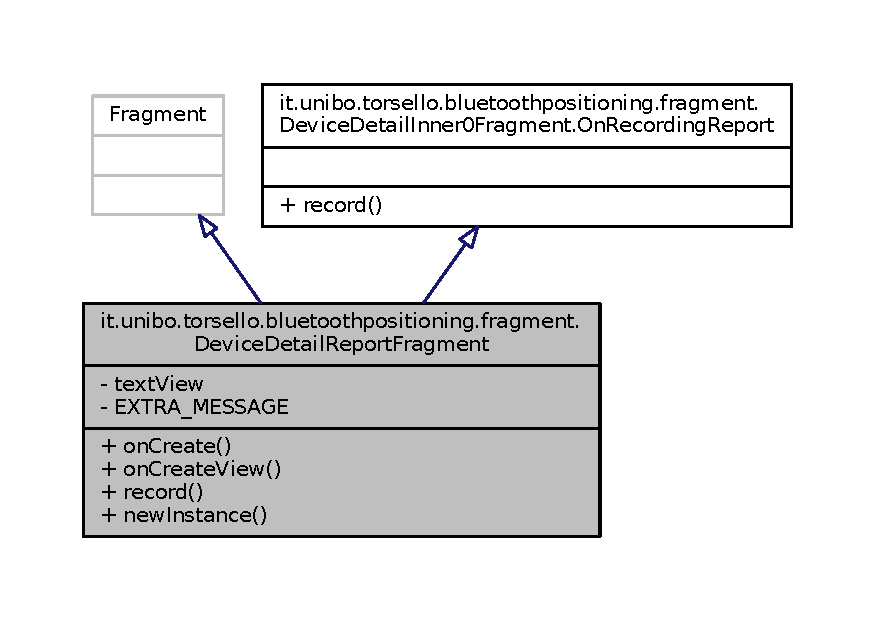
\includegraphics[width=350pt]{classit_1_1unibo_1_1torsello_1_1bluetoothpositioning_1_1fragment_1_1DeviceDetailReportFragment__inherit__graph}
\end{center}
\end{figure}


Diagramma di collaborazione per it.\+unibo.\+torsello.\+bluetoothpositioning.\+fragment.\+Device\+Detail\+Report\+Fragment\+:
\nopagebreak
\begin{figure}[H]
\begin{center}
\leavevmode
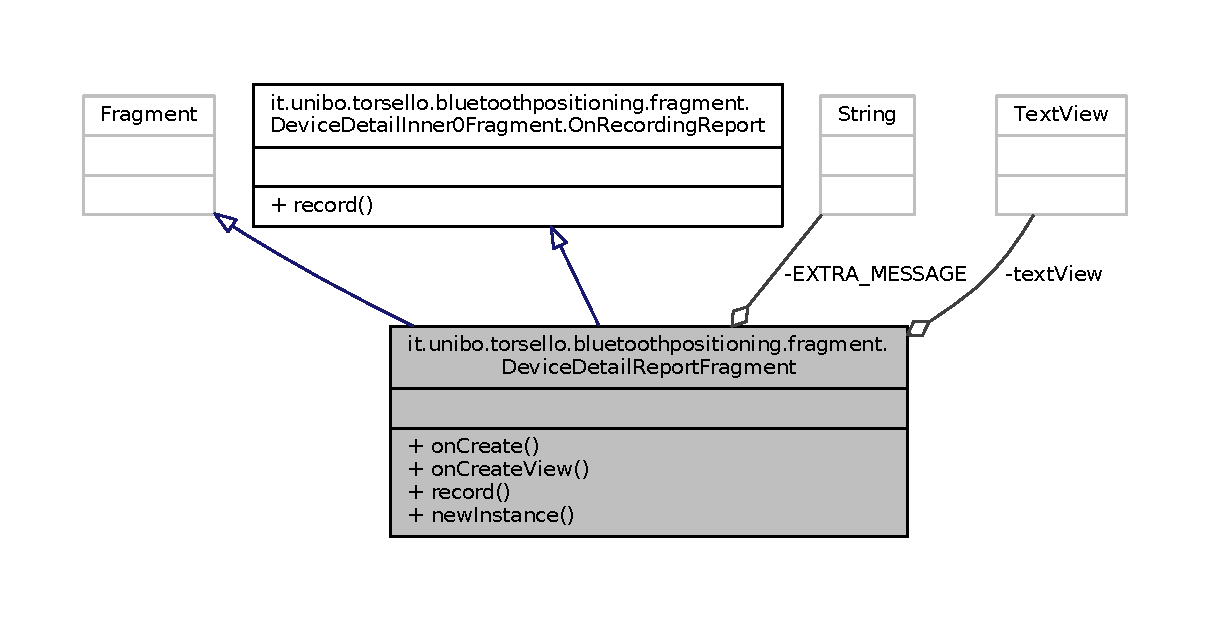
\includegraphics[width=350pt]{classit_1_1unibo_1_1torsello_1_1bluetoothpositioning_1_1fragment_1_1DeviceDetailReportFragment__coll__graph}
\end{center}
\end{figure}
\subsubsection*{Membri pubblici}
\begin{DoxyCompactItemize}
\item 
void \hyperlink{classit_1_1unibo_1_1torsello_1_1bluetoothpositioning_1_1fragment_1_1DeviceDetailReportFragment_a96859a689bc31c69a329d6f2b198c860_a96859a689bc31c69a329d6f2b198c860}{on\+Create} (@Nullable Bundle saved\+Instance\+State)
\item 
View \hyperlink{classit_1_1unibo_1_1torsello_1_1bluetoothpositioning_1_1fragment_1_1DeviceDetailReportFragment_a5aa4df017085deeac5a427fcc63a4fc9_a5aa4df017085deeac5a427fcc63a4fc9}{on\+Create\+View} (Layout\+Inflater inflater, View\+Group container, Bundle saved\+Instance\+State)
\item 
void \hyperlink{classit_1_1unibo_1_1torsello_1_1bluetoothpositioning_1_1fragment_1_1DeviceDetailReportFragment_ae9615d2a2096700befd416d0d8a95f85_ae9615d2a2096700befd416d0d8a95f85}{record} (String new\+Record)
\end{DoxyCompactItemize}
\subsubsection*{Membri pubblici statici}
\begin{DoxyCompactItemize}
\item 
static \hyperlink{classit_1_1unibo_1_1torsello_1_1bluetoothpositioning_1_1fragment_1_1DeviceDetailReportFragment}{Device\+Detail\+Report\+Fragment} \hyperlink{classit_1_1unibo_1_1torsello_1_1bluetoothpositioning_1_1fragment_1_1DeviceDetailReportFragment_a91531900ca550e51463fe827be0d5851_a91531900ca550e51463fe827be0d5851}{new\+Instance} ()
\end{DoxyCompactItemize}
\subsubsection*{Attributi privati}
\begin{DoxyCompactItemize}
\item 
Text\+View \hyperlink{classit_1_1unibo_1_1torsello_1_1bluetoothpositioning_1_1fragment_1_1DeviceDetailReportFragment_a6f00cf8dad82dcd8d6371db58c2235cf_a6f00cf8dad82dcd8d6371db58c2235cf}{text\+View}
\end{DoxyCompactItemize}
\subsubsection*{Attributi privati statici}
\begin{DoxyCompactItemize}
\item 
static final String \hyperlink{classit_1_1unibo_1_1torsello_1_1bluetoothpositioning_1_1fragment_1_1DeviceDetailReportFragment_a906b92cc5a18c57393f96a1fbc1dec15_a906b92cc5a18c57393f96a1fbc1dec15}{E\+X\+T\+R\+A\+\_\+\+M\+E\+S\+S\+A\+GE} = \char`\"{}E\+X\+T\+R\+A\+\_\+\+M\+E\+S\+S\+A\+GE\char`\"{}
\end{DoxyCompactItemize}


\subsubsection{Descrizione dettagliata}
Created by Federico Torsello. \href{mailto:federico.torsello@studio.unibo.it}{\tt federico.\+torsello@studio.\+unibo.\+it} 

\subsubsection{Documentazione delle funzioni membro}
\hypertarget{classit_1_1unibo_1_1torsello_1_1bluetoothpositioning_1_1fragment_1_1DeviceDetailReportFragment_a91531900ca550e51463fe827be0d5851_a91531900ca550e51463fe827be0d5851}{}\label{classit_1_1unibo_1_1torsello_1_1bluetoothpositioning_1_1fragment_1_1DeviceDetailReportFragment_a91531900ca550e51463fe827be0d5851_a91531900ca550e51463fe827be0d5851} 
\index{it\+::unibo\+::torsello\+::bluetoothpositioning\+::fragment\+::\+Device\+Detail\+Report\+Fragment@{it\+::unibo\+::torsello\+::bluetoothpositioning\+::fragment\+::\+Device\+Detail\+Report\+Fragment}!new\+Instance@{new\+Instance}}
\index{new\+Instance@{new\+Instance}!it\+::unibo\+::torsello\+::bluetoothpositioning\+::fragment\+::\+Device\+Detail\+Report\+Fragment@{it\+::unibo\+::torsello\+::bluetoothpositioning\+::fragment\+::\+Device\+Detail\+Report\+Fragment}}
\paragraph{\texorpdfstring{new\+Instance()}{newInstance()}}
{\footnotesize\ttfamily static \hyperlink{classit_1_1unibo_1_1torsello_1_1bluetoothpositioning_1_1fragment_1_1DeviceDetailReportFragment}{Device\+Detail\+Report\+Fragment} it.\+unibo.\+torsello.\+bluetoothpositioning.\+fragment.\+Device\+Detail\+Report\+Fragment.\+new\+Instance (\begin{DoxyParamCaption}{ }\end{DoxyParamCaption})\hspace{0.3cm}{\ttfamily [static]}}


\begin{DoxyCode}
27                                                            \{
28         DeviceDetailReportFragment fragment = \textcolor{keyword}{new} DeviceDetailReportFragment();
29         Bundle args = \textcolor{keyword}{new} Bundle();
30         args.putString(\hyperlink{classit_1_1unibo_1_1torsello_1_1bluetoothpositioning_1_1fragment_1_1DeviceDetailReportFragment_a906b92cc5a18c57393f96a1fbc1dec15_a906b92cc5a18c57393f96a1fbc1dec15}{EXTRA\_MESSAGE}, \textcolor{stringliteral}{"report"});
31         fragment.setArguments(args);
32         \textcolor{keywordflow}{return} fragment;
33     \}
\end{DoxyCode}
\hypertarget{classit_1_1unibo_1_1torsello_1_1bluetoothpositioning_1_1fragment_1_1DeviceDetailReportFragment_a96859a689bc31c69a329d6f2b198c860_a96859a689bc31c69a329d6f2b198c860}{}\label{classit_1_1unibo_1_1torsello_1_1bluetoothpositioning_1_1fragment_1_1DeviceDetailReportFragment_a96859a689bc31c69a329d6f2b198c860_a96859a689bc31c69a329d6f2b198c860} 
\index{it\+::unibo\+::torsello\+::bluetoothpositioning\+::fragment\+::\+Device\+Detail\+Report\+Fragment@{it\+::unibo\+::torsello\+::bluetoothpositioning\+::fragment\+::\+Device\+Detail\+Report\+Fragment}!on\+Create@{on\+Create}}
\index{on\+Create@{on\+Create}!it\+::unibo\+::torsello\+::bluetoothpositioning\+::fragment\+::\+Device\+Detail\+Report\+Fragment@{it\+::unibo\+::torsello\+::bluetoothpositioning\+::fragment\+::\+Device\+Detail\+Report\+Fragment}}
\paragraph{\texorpdfstring{on\+Create()}{onCreate()}}
{\footnotesize\ttfamily void it.\+unibo.\+torsello.\+bluetoothpositioning.\+fragment.\+Device\+Detail\+Report\+Fragment.\+on\+Create (\begin{DoxyParamCaption}\item[{@Nullable Bundle}]{saved\+Instance\+State }\end{DoxyParamCaption})}


\begin{DoxyCode}
36                                                               \{
37         super.onCreate(savedInstanceState);
38 
39     \}
\end{DoxyCode}
\hypertarget{classit_1_1unibo_1_1torsello_1_1bluetoothpositioning_1_1fragment_1_1DeviceDetailReportFragment_a5aa4df017085deeac5a427fcc63a4fc9_a5aa4df017085deeac5a427fcc63a4fc9}{}\label{classit_1_1unibo_1_1torsello_1_1bluetoothpositioning_1_1fragment_1_1DeviceDetailReportFragment_a5aa4df017085deeac5a427fcc63a4fc9_a5aa4df017085deeac5a427fcc63a4fc9} 
\index{it\+::unibo\+::torsello\+::bluetoothpositioning\+::fragment\+::\+Device\+Detail\+Report\+Fragment@{it\+::unibo\+::torsello\+::bluetoothpositioning\+::fragment\+::\+Device\+Detail\+Report\+Fragment}!on\+Create\+View@{on\+Create\+View}}
\index{on\+Create\+View@{on\+Create\+View}!it\+::unibo\+::torsello\+::bluetoothpositioning\+::fragment\+::\+Device\+Detail\+Report\+Fragment@{it\+::unibo\+::torsello\+::bluetoothpositioning\+::fragment\+::\+Device\+Detail\+Report\+Fragment}}
\paragraph{\texorpdfstring{on\+Create\+View()}{onCreateView()}}
{\footnotesize\ttfamily View it.\+unibo.\+torsello.\+bluetoothpositioning.\+fragment.\+Device\+Detail\+Report\+Fragment.\+on\+Create\+View (\begin{DoxyParamCaption}\item[{Layout\+Inflater}]{inflater,  }\item[{View\+Group}]{container,  }\item[{Bundle}]{saved\+Instance\+State }\end{DoxyParamCaption})}


\begin{DoxyCode}
43                                                         \{
44         \textcolor{comment}{// Inflate the layout for this fragment}
45         \textcolor{keyword}{final} View root = inflater.inflate(R.layout.fragment\_device\_detail\_report, container, \textcolor{keyword}{false});
46 
47         \hyperlink{classit_1_1unibo_1_1torsello_1_1bluetoothpositioning_1_1fragment_1_1DeviceDetailReportFragment_a6f00cf8dad82dcd8d6371db58c2235cf_a6f00cf8dad82dcd8d6371db58c2235cf}{textView} = (TextView) root.findViewById(R.id.textView\_report);
48 
49         \textcolor{keywordflow}{return} root;
50     \}
\end{DoxyCode}
\hypertarget{classit_1_1unibo_1_1torsello_1_1bluetoothpositioning_1_1fragment_1_1DeviceDetailReportFragment_ae9615d2a2096700befd416d0d8a95f85_ae9615d2a2096700befd416d0d8a95f85}{}\label{classit_1_1unibo_1_1torsello_1_1bluetoothpositioning_1_1fragment_1_1DeviceDetailReportFragment_ae9615d2a2096700befd416d0d8a95f85_ae9615d2a2096700befd416d0d8a95f85} 
\index{it\+::unibo\+::torsello\+::bluetoothpositioning\+::fragment\+::\+Device\+Detail\+Report\+Fragment@{it\+::unibo\+::torsello\+::bluetoothpositioning\+::fragment\+::\+Device\+Detail\+Report\+Fragment}!record@{record}}
\index{record@{record}!it\+::unibo\+::torsello\+::bluetoothpositioning\+::fragment\+::\+Device\+Detail\+Report\+Fragment@{it\+::unibo\+::torsello\+::bluetoothpositioning\+::fragment\+::\+Device\+Detail\+Report\+Fragment}}
\paragraph{\texorpdfstring{record()}{record()}}
{\footnotesize\ttfamily void it.\+unibo.\+torsello.\+bluetoothpositioning.\+fragment.\+Device\+Detail\+Report\+Fragment.\+record (\begin{DoxyParamCaption}\item[{String}]{new\+Record }\end{DoxyParamCaption})}



Implementa \hyperlink{interfaceit_1_1unibo_1_1torsello_1_1bluetoothpositioning_1_1fragment_1_1DeviceDetailInner0Fragment_1_1OnRecordingReport_a63fd189046ae9d716c19b152957f6c74_a63fd189046ae9d716c19b152957f6c74}{it.\+unibo.\+torsello.\+bluetoothpositioning.\+fragment.\+Device\+Detail\+Inner0\+Fragment.\+On\+Recording\+Report}.


\begin{DoxyCode}
53                                          \{
54         \hyperlink{classit_1_1unibo_1_1torsello_1_1bluetoothpositioning_1_1fragment_1_1DeviceDetailReportFragment_a6f00cf8dad82dcd8d6371db58c2235cf_a6f00cf8dad82dcd8d6371db58c2235cf}{textView}.setText(newRecord);
55     \}
\end{DoxyCode}


\subsubsection{Documentazione dei membri dato}
\hypertarget{classit_1_1unibo_1_1torsello_1_1bluetoothpositioning_1_1fragment_1_1DeviceDetailReportFragment_a906b92cc5a18c57393f96a1fbc1dec15_a906b92cc5a18c57393f96a1fbc1dec15}{}\label{classit_1_1unibo_1_1torsello_1_1bluetoothpositioning_1_1fragment_1_1DeviceDetailReportFragment_a906b92cc5a18c57393f96a1fbc1dec15_a906b92cc5a18c57393f96a1fbc1dec15} 
\index{it\+::unibo\+::torsello\+::bluetoothpositioning\+::fragment\+::\+Device\+Detail\+Report\+Fragment@{it\+::unibo\+::torsello\+::bluetoothpositioning\+::fragment\+::\+Device\+Detail\+Report\+Fragment}!E\+X\+T\+R\+A\+\_\+\+M\+E\+S\+S\+A\+GE@{E\+X\+T\+R\+A\+\_\+\+M\+E\+S\+S\+A\+GE}}
\index{E\+X\+T\+R\+A\+\_\+\+M\+E\+S\+S\+A\+GE@{E\+X\+T\+R\+A\+\_\+\+M\+E\+S\+S\+A\+GE}!it\+::unibo\+::torsello\+::bluetoothpositioning\+::fragment\+::\+Device\+Detail\+Report\+Fragment@{it\+::unibo\+::torsello\+::bluetoothpositioning\+::fragment\+::\+Device\+Detail\+Report\+Fragment}}
\paragraph{\texorpdfstring{E\+X\+T\+R\+A\+\_\+\+M\+E\+S\+S\+A\+GE}{EXTRA\_MESSAGE}}
{\footnotesize\ttfamily final String it.\+unibo.\+torsello.\+bluetoothpositioning.\+fragment.\+Device\+Detail\+Report\+Fragment.\+E\+X\+T\+R\+A\+\_\+\+M\+E\+S\+S\+A\+GE = \char`\"{}E\+X\+T\+R\+A\+\_\+\+M\+E\+S\+S\+A\+GE\char`\"{}\hspace{0.3cm}{\ttfamily [static]}, {\ttfamily [private]}}

\hypertarget{classit_1_1unibo_1_1torsello_1_1bluetoothpositioning_1_1fragment_1_1DeviceDetailReportFragment_a6f00cf8dad82dcd8d6371db58c2235cf_a6f00cf8dad82dcd8d6371db58c2235cf}{}\label{classit_1_1unibo_1_1torsello_1_1bluetoothpositioning_1_1fragment_1_1DeviceDetailReportFragment_a6f00cf8dad82dcd8d6371db58c2235cf_a6f00cf8dad82dcd8d6371db58c2235cf} 
\index{it\+::unibo\+::torsello\+::bluetoothpositioning\+::fragment\+::\+Device\+Detail\+Report\+Fragment@{it\+::unibo\+::torsello\+::bluetoothpositioning\+::fragment\+::\+Device\+Detail\+Report\+Fragment}!text\+View@{text\+View}}
\index{text\+View@{text\+View}!it\+::unibo\+::torsello\+::bluetoothpositioning\+::fragment\+::\+Device\+Detail\+Report\+Fragment@{it\+::unibo\+::torsello\+::bluetoothpositioning\+::fragment\+::\+Device\+Detail\+Report\+Fragment}}
\paragraph{\texorpdfstring{text\+View}{textView}}
{\footnotesize\ttfamily Text\+View it.\+unibo.\+torsello.\+bluetoothpositioning.\+fragment.\+Device\+Detail\+Report\+Fragment.\+text\+View\hspace{0.3cm}{\ttfamily [private]}}



La documentazione per questa classe è stata generata a partire dal seguente file\+:\begin{DoxyCompactItemize}
\item 
\hyperlink{DeviceDetailReportFragment_8java}{Device\+Detail\+Report\+Fragment.\+java}\end{DoxyCompactItemize}

\hypertarget{classit_1_1unibo_1_1torsello_1_1bluetoothpositioning_1_1fragment_1_1DeviceDetailResumeFragment}{}\subsection{Riferimenti per la classe it.\+unibo.\+torsello.\+bluetoothpositioning.\+fragment.\+Device\+Detail\+Resume\+Fragment}
\label{classit_1_1unibo_1_1torsello_1_1bluetoothpositioning_1_1fragment_1_1DeviceDetailResumeFragment}\index{it.\+unibo.\+torsello.\+bluetoothpositioning.\+fragment.\+Device\+Detail\+Resume\+Fragment@{it.\+unibo.\+torsello.\+bluetoothpositioning.\+fragment.\+Device\+Detail\+Resume\+Fragment}}


Diagramma delle classi per it.\+unibo.\+torsello.\+bluetoothpositioning.\+fragment.\+Device\+Detail\+Resume\+Fragment
\nopagebreak
\begin{figure}[H]
\begin{center}
\leavevmode
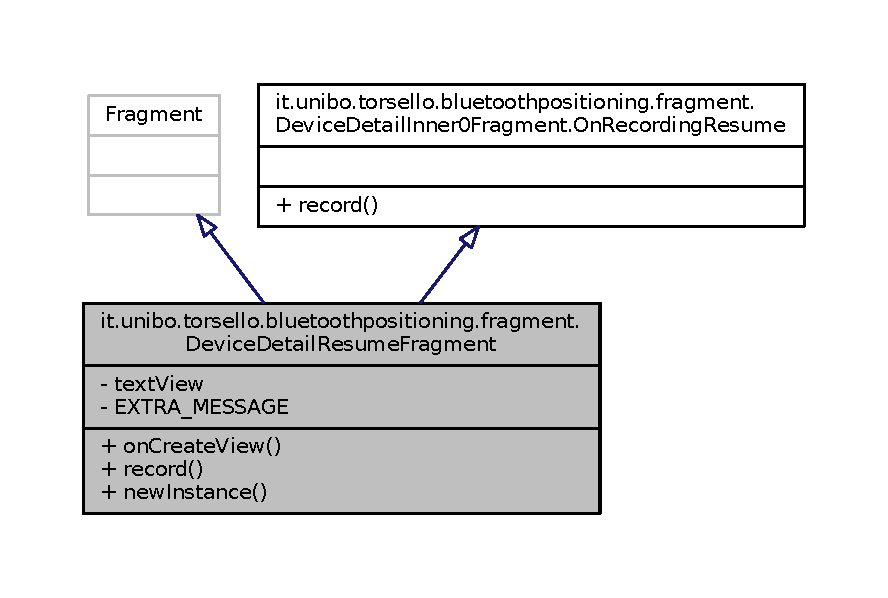
\includegraphics[width=350pt]{classit_1_1unibo_1_1torsello_1_1bluetoothpositioning_1_1fragment_1_1DeviceDetailResumeFragment__inherit__graph}
\end{center}
\end{figure}


Diagramma di collaborazione per it.\+unibo.\+torsello.\+bluetoothpositioning.\+fragment.\+Device\+Detail\+Resume\+Fragment\+:
\nopagebreak
\begin{figure}[H]
\begin{center}
\leavevmode
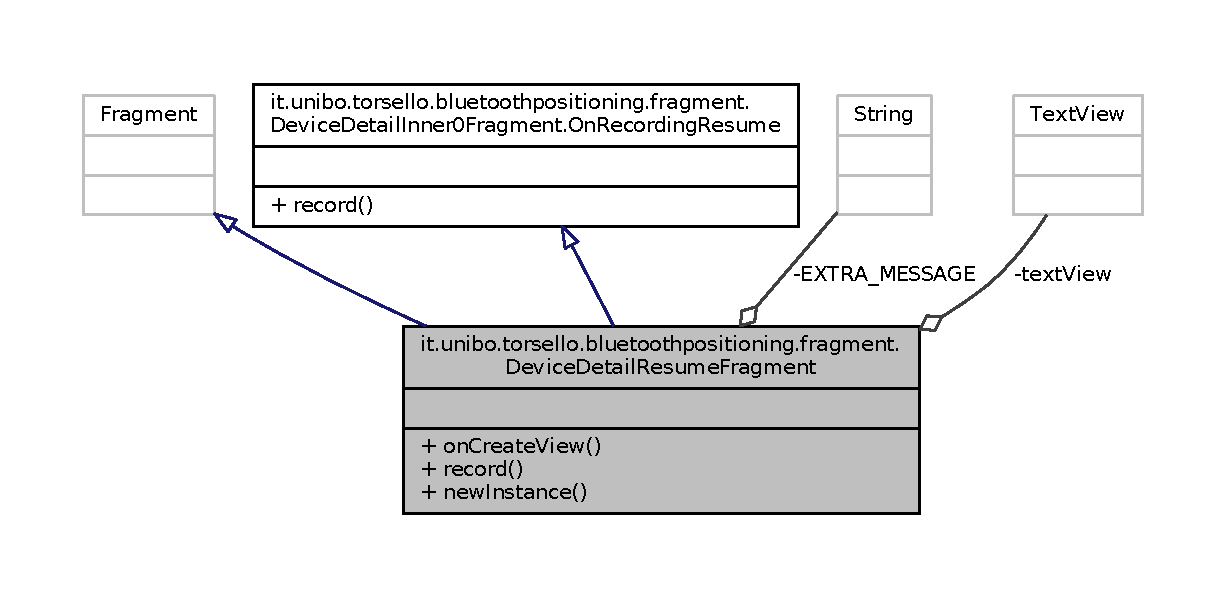
\includegraphics[width=350pt]{classit_1_1unibo_1_1torsello_1_1bluetoothpositioning_1_1fragment_1_1DeviceDetailResumeFragment__coll__graph}
\end{center}
\end{figure}
\subsubsection*{Membri pubblici}
\begin{DoxyCompactItemize}
\item 
View \hyperlink{classit_1_1unibo_1_1torsello_1_1bluetoothpositioning_1_1fragment_1_1DeviceDetailResumeFragment_ac6332cf63f2ea0f1276b031c1b17537f_ac6332cf63f2ea0f1276b031c1b17537f}{on\+Create\+View} (Layout\+Inflater inflater, View\+Group container, Bundle saved\+Instance\+State)
\item 
void \hyperlink{classit_1_1unibo_1_1torsello_1_1bluetoothpositioning_1_1fragment_1_1DeviceDetailResumeFragment_aa4b3952d75b693caa46309f0f2ca05b4_aa4b3952d75b693caa46309f0f2ca05b4}{record} (String new\+Record)
\end{DoxyCompactItemize}
\subsubsection*{Membri pubblici statici}
\begin{DoxyCompactItemize}
\item 
static \hyperlink{classit_1_1unibo_1_1torsello_1_1bluetoothpositioning_1_1fragment_1_1DeviceDetailResumeFragment}{Device\+Detail\+Resume\+Fragment} \hyperlink{classit_1_1unibo_1_1torsello_1_1bluetoothpositioning_1_1fragment_1_1DeviceDetailResumeFragment_aab49893918bdd656328e6ee8021e1c52_aab49893918bdd656328e6ee8021e1c52}{new\+Instance} ()
\end{DoxyCompactItemize}
\subsubsection*{Attributi privati}
\begin{DoxyCompactItemize}
\item 
Text\+View \hyperlink{classit_1_1unibo_1_1torsello_1_1bluetoothpositioning_1_1fragment_1_1DeviceDetailResumeFragment_a0ce36645eb31d9ab981a9dfeef206ada_a0ce36645eb31d9ab981a9dfeef206ada}{text\+View}
\end{DoxyCompactItemize}
\subsubsection*{Attributi privati statici}
\begin{DoxyCompactItemize}
\item 
static final String \hyperlink{classit_1_1unibo_1_1torsello_1_1bluetoothpositioning_1_1fragment_1_1DeviceDetailResumeFragment_a26b6bb100efe8bbb74e10fbd8deca47f_a26b6bb100efe8bbb74e10fbd8deca47f}{E\+X\+T\+R\+A\+\_\+\+M\+E\+S\+S\+A\+GE} = \char`\"{}E\+X\+T\+R\+A\+\_\+\+M\+E\+S\+S\+A\+GE\char`\"{}
\end{DoxyCompactItemize}


\subsubsection{Descrizione dettagliata}
Created by federico on 12/10/16. 

\subsubsection{Documentazione delle funzioni membro}
\hypertarget{classit_1_1unibo_1_1torsello_1_1bluetoothpositioning_1_1fragment_1_1DeviceDetailResumeFragment_aab49893918bdd656328e6ee8021e1c52_aab49893918bdd656328e6ee8021e1c52}{}\label{classit_1_1unibo_1_1torsello_1_1bluetoothpositioning_1_1fragment_1_1DeviceDetailResumeFragment_aab49893918bdd656328e6ee8021e1c52_aab49893918bdd656328e6ee8021e1c52} 
\index{it\+::unibo\+::torsello\+::bluetoothpositioning\+::fragment\+::\+Device\+Detail\+Resume\+Fragment@{it\+::unibo\+::torsello\+::bluetoothpositioning\+::fragment\+::\+Device\+Detail\+Resume\+Fragment}!new\+Instance@{new\+Instance}}
\index{new\+Instance@{new\+Instance}!it\+::unibo\+::torsello\+::bluetoothpositioning\+::fragment\+::\+Device\+Detail\+Resume\+Fragment@{it\+::unibo\+::torsello\+::bluetoothpositioning\+::fragment\+::\+Device\+Detail\+Resume\+Fragment}}
\paragraph{\texorpdfstring{new\+Instance()}{newInstance()}}
{\footnotesize\ttfamily static \hyperlink{classit_1_1unibo_1_1torsello_1_1bluetoothpositioning_1_1fragment_1_1DeviceDetailResumeFragment}{Device\+Detail\+Resume\+Fragment} it.\+unibo.\+torsello.\+bluetoothpositioning.\+fragment.\+Device\+Detail\+Resume\+Fragment.\+new\+Instance (\begin{DoxyParamCaption}{ }\end{DoxyParamCaption})\hspace{0.3cm}{\ttfamily [static]}}


\begin{DoxyCode}
27                                                            \{
28         DeviceDetailResumeFragment fragment = \textcolor{keyword}{new} DeviceDetailResumeFragment();
29         Bundle args = \textcolor{keyword}{new} Bundle();
30         args.putString(\hyperlink{classit_1_1unibo_1_1torsello_1_1bluetoothpositioning_1_1fragment_1_1DeviceDetailResumeFragment_a26b6bb100efe8bbb74e10fbd8deca47f_a26b6bb100efe8bbb74e10fbd8deca47f}{EXTRA\_MESSAGE}, \textcolor{stringliteral}{"Resume"});
31         fragment.setArguments(args);
32         \textcolor{keywordflow}{return} fragment;
33     \}
\end{DoxyCode}
\hypertarget{classit_1_1unibo_1_1torsello_1_1bluetoothpositioning_1_1fragment_1_1DeviceDetailResumeFragment_ac6332cf63f2ea0f1276b031c1b17537f_ac6332cf63f2ea0f1276b031c1b17537f}{}\label{classit_1_1unibo_1_1torsello_1_1bluetoothpositioning_1_1fragment_1_1DeviceDetailResumeFragment_ac6332cf63f2ea0f1276b031c1b17537f_ac6332cf63f2ea0f1276b031c1b17537f} 
\index{it\+::unibo\+::torsello\+::bluetoothpositioning\+::fragment\+::\+Device\+Detail\+Resume\+Fragment@{it\+::unibo\+::torsello\+::bluetoothpositioning\+::fragment\+::\+Device\+Detail\+Resume\+Fragment}!on\+Create\+View@{on\+Create\+View}}
\index{on\+Create\+View@{on\+Create\+View}!it\+::unibo\+::torsello\+::bluetoothpositioning\+::fragment\+::\+Device\+Detail\+Resume\+Fragment@{it\+::unibo\+::torsello\+::bluetoothpositioning\+::fragment\+::\+Device\+Detail\+Resume\+Fragment}}
\paragraph{\texorpdfstring{on\+Create\+View()}{onCreateView()}}
{\footnotesize\ttfamily View it.\+unibo.\+torsello.\+bluetoothpositioning.\+fragment.\+Device\+Detail\+Resume\+Fragment.\+on\+Create\+View (\begin{DoxyParamCaption}\item[{Layout\+Inflater}]{inflater,  }\item[{View\+Group}]{container,  }\item[{Bundle}]{saved\+Instance\+State }\end{DoxyParamCaption})}


\begin{DoxyCode}
37                                                         \{
38         \textcolor{comment}{// Inflate the layout for this fragment}
39         \textcolor{keyword}{final} View root = inflater.inflate(R.layout.fragment\_device\_detail\_resume, container, \textcolor{keyword}{false});
40 
41         \hyperlink{classit_1_1unibo_1_1torsello_1_1bluetoothpositioning_1_1fragment_1_1DeviceDetailResumeFragment_a0ce36645eb31d9ab981a9dfeef206ada_a0ce36645eb31d9ab981a9dfeef206ada}{textView} = (TextView) root.findViewById(R.id.textView\_resume);
42 
43         \textcolor{keywordflow}{return} root;
44     \}
\end{DoxyCode}
\hypertarget{classit_1_1unibo_1_1torsello_1_1bluetoothpositioning_1_1fragment_1_1DeviceDetailResumeFragment_aa4b3952d75b693caa46309f0f2ca05b4_aa4b3952d75b693caa46309f0f2ca05b4}{}\label{classit_1_1unibo_1_1torsello_1_1bluetoothpositioning_1_1fragment_1_1DeviceDetailResumeFragment_aa4b3952d75b693caa46309f0f2ca05b4_aa4b3952d75b693caa46309f0f2ca05b4} 
\index{it\+::unibo\+::torsello\+::bluetoothpositioning\+::fragment\+::\+Device\+Detail\+Resume\+Fragment@{it\+::unibo\+::torsello\+::bluetoothpositioning\+::fragment\+::\+Device\+Detail\+Resume\+Fragment}!record@{record}}
\index{record@{record}!it\+::unibo\+::torsello\+::bluetoothpositioning\+::fragment\+::\+Device\+Detail\+Resume\+Fragment@{it\+::unibo\+::torsello\+::bluetoothpositioning\+::fragment\+::\+Device\+Detail\+Resume\+Fragment}}
\paragraph{\texorpdfstring{record()}{record()}}
{\footnotesize\ttfamily void it.\+unibo.\+torsello.\+bluetoothpositioning.\+fragment.\+Device\+Detail\+Resume\+Fragment.\+record (\begin{DoxyParamCaption}\item[{String}]{new\+Record }\end{DoxyParamCaption})}



Implementa \hyperlink{interfaceit_1_1unibo_1_1torsello_1_1bluetoothpositioning_1_1fragment_1_1DeviceDetailInner0Fragment_1_1OnRecordingResume_a68528e5fbaa02cb01776eba68da833d8_a68528e5fbaa02cb01776eba68da833d8}{it.\+unibo.\+torsello.\+bluetoothpositioning.\+fragment.\+Device\+Detail\+Inner0\+Fragment.\+On\+Recording\+Resume}.


\begin{DoxyCode}
47                                          \{
48         \hyperlink{classit_1_1unibo_1_1torsello_1_1bluetoothpositioning_1_1fragment_1_1DeviceDetailResumeFragment_a0ce36645eb31d9ab981a9dfeef206ada_a0ce36645eb31d9ab981a9dfeef206ada}{textView}.setText(newRecord);
49     \}
\end{DoxyCode}


\subsubsection{Documentazione dei membri dato}
\hypertarget{classit_1_1unibo_1_1torsello_1_1bluetoothpositioning_1_1fragment_1_1DeviceDetailResumeFragment_a26b6bb100efe8bbb74e10fbd8deca47f_a26b6bb100efe8bbb74e10fbd8deca47f}{}\label{classit_1_1unibo_1_1torsello_1_1bluetoothpositioning_1_1fragment_1_1DeviceDetailResumeFragment_a26b6bb100efe8bbb74e10fbd8deca47f_a26b6bb100efe8bbb74e10fbd8deca47f} 
\index{it\+::unibo\+::torsello\+::bluetoothpositioning\+::fragment\+::\+Device\+Detail\+Resume\+Fragment@{it\+::unibo\+::torsello\+::bluetoothpositioning\+::fragment\+::\+Device\+Detail\+Resume\+Fragment}!E\+X\+T\+R\+A\+\_\+\+M\+E\+S\+S\+A\+GE@{E\+X\+T\+R\+A\+\_\+\+M\+E\+S\+S\+A\+GE}}
\index{E\+X\+T\+R\+A\+\_\+\+M\+E\+S\+S\+A\+GE@{E\+X\+T\+R\+A\+\_\+\+M\+E\+S\+S\+A\+GE}!it\+::unibo\+::torsello\+::bluetoothpositioning\+::fragment\+::\+Device\+Detail\+Resume\+Fragment@{it\+::unibo\+::torsello\+::bluetoothpositioning\+::fragment\+::\+Device\+Detail\+Resume\+Fragment}}
\paragraph{\texorpdfstring{E\+X\+T\+R\+A\+\_\+\+M\+E\+S\+S\+A\+GE}{EXTRA\_MESSAGE}}
{\footnotesize\ttfamily final String it.\+unibo.\+torsello.\+bluetoothpositioning.\+fragment.\+Device\+Detail\+Resume\+Fragment.\+E\+X\+T\+R\+A\+\_\+\+M\+E\+S\+S\+A\+GE = \char`\"{}E\+X\+T\+R\+A\+\_\+\+M\+E\+S\+S\+A\+GE\char`\"{}\hspace{0.3cm}{\ttfamily [static]}, {\ttfamily [private]}}

\hypertarget{classit_1_1unibo_1_1torsello_1_1bluetoothpositioning_1_1fragment_1_1DeviceDetailResumeFragment_a0ce36645eb31d9ab981a9dfeef206ada_a0ce36645eb31d9ab981a9dfeef206ada}{}\label{classit_1_1unibo_1_1torsello_1_1bluetoothpositioning_1_1fragment_1_1DeviceDetailResumeFragment_a0ce36645eb31d9ab981a9dfeef206ada_a0ce36645eb31d9ab981a9dfeef206ada} 
\index{it\+::unibo\+::torsello\+::bluetoothpositioning\+::fragment\+::\+Device\+Detail\+Resume\+Fragment@{it\+::unibo\+::torsello\+::bluetoothpositioning\+::fragment\+::\+Device\+Detail\+Resume\+Fragment}!text\+View@{text\+View}}
\index{text\+View@{text\+View}!it\+::unibo\+::torsello\+::bluetoothpositioning\+::fragment\+::\+Device\+Detail\+Resume\+Fragment@{it\+::unibo\+::torsello\+::bluetoothpositioning\+::fragment\+::\+Device\+Detail\+Resume\+Fragment}}
\paragraph{\texorpdfstring{text\+View}{textView}}
{\footnotesize\ttfamily Text\+View it.\+unibo.\+torsello.\+bluetoothpositioning.\+fragment.\+Device\+Detail\+Resume\+Fragment.\+text\+View\hspace{0.3cm}{\ttfamily [private]}}



La documentazione per questa classe è stata generata a partire dal seguente file\+:\begin{DoxyCompactItemize}
\item 
\hyperlink{DeviceDetailResumeFragment_8java}{Device\+Detail\+Resume\+Fragment.\+java}\end{DoxyCompactItemize}

\hypertarget{classit_1_1unibo_1_1torsello_1_1bluetoothpositioning_1_1fragment_1_1DeviceListFragment}{}\subsection{Riferimenti per la classe it.\+unibo.\+torsello.\+bluetoothpositioning.\+fragment.\+Device\+List\+Fragment}
\label{classit_1_1unibo_1_1torsello_1_1bluetoothpositioning_1_1fragment_1_1DeviceListFragment}\index{it.\+unibo.\+torsello.\+bluetoothpositioning.\+fragment.\+Device\+List\+Fragment@{it.\+unibo.\+torsello.\+bluetoothpositioning.\+fragment.\+Device\+List\+Fragment}}


Diagramma delle classi per it.\+unibo.\+torsello.\+bluetoothpositioning.\+fragment.\+Device\+List\+Fragment
\nopagebreak
\begin{figure}[H]
\begin{center}
\leavevmode
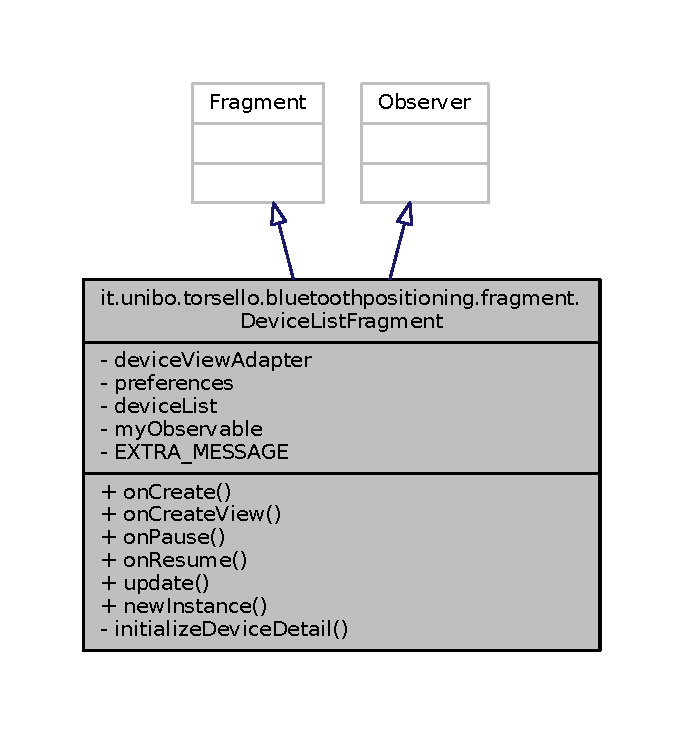
\includegraphics[width=328pt]{classit_1_1unibo_1_1torsello_1_1bluetoothpositioning_1_1fragment_1_1DeviceListFragment__inherit__graph}
\end{center}
\end{figure}


Diagramma di collaborazione per it.\+unibo.\+torsello.\+bluetoothpositioning.\+fragment.\+Device\+List\+Fragment\+:
\nopagebreak
\begin{figure}[H]
\begin{center}
\leavevmode
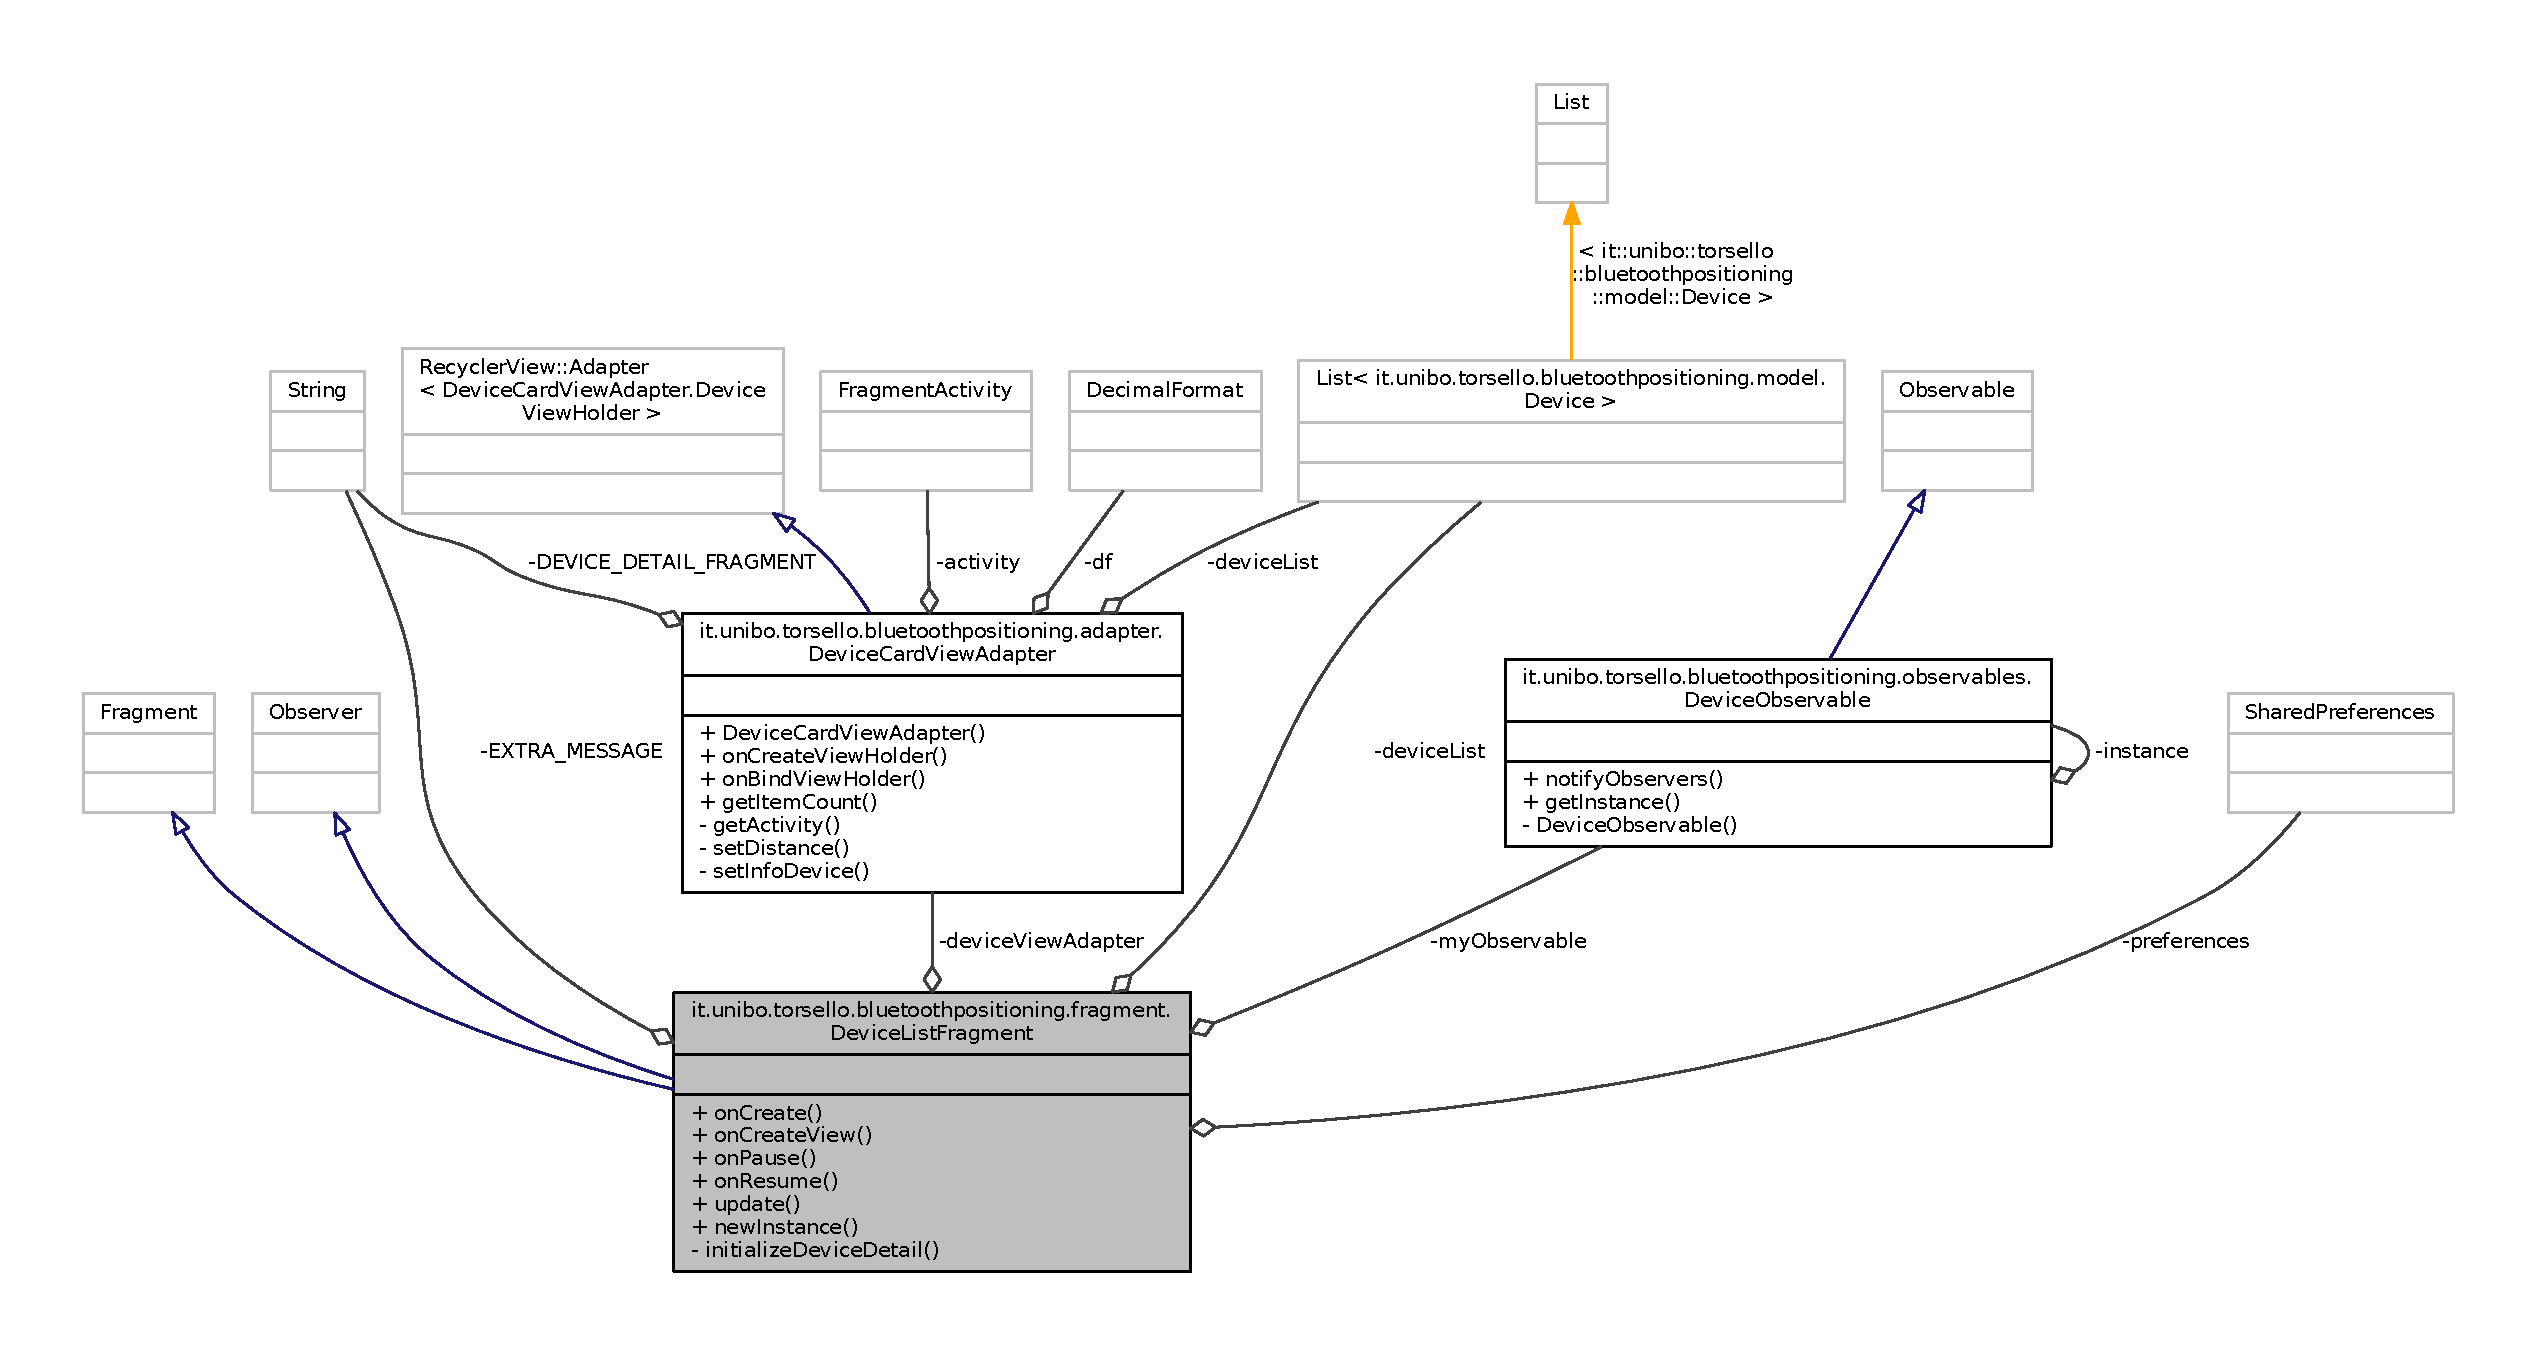
\includegraphics[width=350pt]{classit_1_1unibo_1_1torsello_1_1bluetoothpositioning_1_1fragment_1_1DeviceListFragment__coll__graph}
\end{center}
\end{figure}
\subsubsection*{Membri pubblici}
\begin{DoxyCompactItemize}
\item 
void \hyperlink{classit_1_1unibo_1_1torsello_1_1bluetoothpositioning_1_1fragment_1_1DeviceListFragment_a6dc90ae91b0b8d10260a2d55ca193db6_a6dc90ae91b0b8d10260a2d55ca193db6}{on\+Create} (@Nullable Bundle saved\+Instance\+State)
\item 
View \hyperlink{classit_1_1unibo_1_1torsello_1_1bluetoothpositioning_1_1fragment_1_1DeviceListFragment_ae359841af9f15a6e1ccea49656a2c6aa_ae359841af9f15a6e1ccea49656a2c6aa}{on\+Create\+View} (Layout\+Inflater inflater, View\+Group container, Bundle saved\+Instance\+State)
\item 
void \hyperlink{classit_1_1unibo_1_1torsello_1_1bluetoothpositioning_1_1fragment_1_1DeviceListFragment_a664ab33df789cde4831b60b83ec31436_a664ab33df789cde4831b60b83ec31436}{on\+Pause} ()
\item 
void \hyperlink{classit_1_1unibo_1_1torsello_1_1bluetoothpositioning_1_1fragment_1_1DeviceListFragment_ab70d378c12ff5e9ffab0a61548119282_ab70d378c12ff5e9ffab0a61548119282}{on\+Resume} ()
\item 
void \hyperlink{classit_1_1unibo_1_1torsello_1_1bluetoothpositioning_1_1fragment_1_1DeviceListFragment_a5c8153bcb9d24c048d8f605f8f280557_a5c8153bcb9d24c048d8f605f8f280557}{update} (Observable o, Object arg)
\end{DoxyCompactItemize}
\subsubsection*{Membri pubblici statici}
\begin{DoxyCompactItemize}
\item 
static \hyperlink{classit_1_1unibo_1_1torsello_1_1bluetoothpositioning_1_1fragment_1_1DeviceListFragment}{Device\+List\+Fragment} \hyperlink{classit_1_1unibo_1_1torsello_1_1bluetoothpositioning_1_1fragment_1_1DeviceListFragment_aca684c7fd0da8c25be68ef7e5f80b871_aca684c7fd0da8c25be68ef7e5f80b871}{new\+Instance} ()
\end{DoxyCompactItemize}
\subsubsection*{Membri privati}
\begin{DoxyCompactItemize}
\item 
void \hyperlink{classit_1_1unibo_1_1torsello_1_1bluetoothpositioning_1_1fragment_1_1DeviceListFragment_aafeba576519b4e419c2d5274d5a65133_aafeba576519b4e419c2d5274d5a65133}{initialize\+Device\+Detail} (View root)
\end{DoxyCompactItemize}
\subsubsection*{Attributi privati}
\begin{DoxyCompactItemize}
\item 
\hyperlink{classit_1_1unibo_1_1torsello_1_1bluetoothpositioning_1_1adapter_1_1DeviceCardViewAdapter}{Device\+Card\+View\+Adapter} \hyperlink{classit_1_1unibo_1_1torsello_1_1bluetoothpositioning_1_1fragment_1_1DeviceListFragment_af33bdf009badab587a755e2e40dc4bc5_af33bdf009badab587a755e2e40dc4bc5}{device\+View\+Adapter}
\item 
Shared\+Preferences \hyperlink{classit_1_1unibo_1_1torsello_1_1bluetoothpositioning_1_1fragment_1_1DeviceListFragment_a3f583494281dbe65b3e76c28b5facbe7_a3f583494281dbe65b3e76c28b5facbe7}{preferences}
\item 
List$<$ \hyperlink{classit_1_1unibo_1_1torsello_1_1bluetoothpositioning_1_1model_1_1Device}{Device} $>$ \hyperlink{classit_1_1unibo_1_1torsello_1_1bluetoothpositioning_1_1fragment_1_1DeviceListFragment_a19a4a9cff961d3c319aaa80d5412a9a6_a19a4a9cff961d3c319aaa80d5412a9a6}{device\+List}
\item 
\hyperlink{classit_1_1unibo_1_1torsello_1_1bluetoothpositioning_1_1observables_1_1DeviceObservable}{Device\+Observable} \hyperlink{classit_1_1unibo_1_1torsello_1_1bluetoothpositioning_1_1fragment_1_1DeviceListFragment_a6a78ac6c8b7bc5b91a5966c341305b62_a6a78ac6c8b7bc5b91a5966c341305b62}{my\+Observable}
\end{DoxyCompactItemize}
\subsubsection*{Attributi privati statici}
\begin{DoxyCompactItemize}
\item 
static final String \hyperlink{classit_1_1unibo_1_1torsello_1_1bluetoothpositioning_1_1fragment_1_1DeviceListFragment_a6124d6f80d72149642440bb5910c2a53_a6124d6f80d72149642440bb5910c2a53}{E\+X\+T\+R\+A\+\_\+\+M\+E\+S\+S\+A\+GE} = \char`\"{}E\+X\+T\+R\+A\+\_\+\+M\+E\+S\+S\+A\+GE\char`\"{}
\end{DoxyCompactItemize}


\subsubsection{Descrizione dettagliata}
Created by Federico Torsello. \href{mailto:federico.torsello@studio.unibo.it}{\tt federico.\+torsello@studio.\+unibo.\+it} 

\subsubsection{Documentazione delle funzioni membro}
\hypertarget{classit_1_1unibo_1_1torsello_1_1bluetoothpositioning_1_1fragment_1_1DeviceListFragment_aafeba576519b4e419c2d5274d5a65133_aafeba576519b4e419c2d5274d5a65133}{}\label{classit_1_1unibo_1_1torsello_1_1bluetoothpositioning_1_1fragment_1_1DeviceListFragment_aafeba576519b4e419c2d5274d5a65133_aafeba576519b4e419c2d5274d5a65133} 
\index{it\+::unibo\+::torsello\+::bluetoothpositioning\+::fragment\+::\+Device\+List\+Fragment@{it\+::unibo\+::torsello\+::bluetoothpositioning\+::fragment\+::\+Device\+List\+Fragment}!initialize\+Device\+Detail@{initialize\+Device\+Detail}}
\index{initialize\+Device\+Detail@{initialize\+Device\+Detail}!it\+::unibo\+::torsello\+::bluetoothpositioning\+::fragment\+::\+Device\+List\+Fragment@{it\+::unibo\+::torsello\+::bluetoothpositioning\+::fragment\+::\+Device\+List\+Fragment}}
\paragraph{\texorpdfstring{initialize\+Device\+Detail()}{initializeDeviceDetail()}}
{\footnotesize\ttfamily void it.\+unibo.\+torsello.\+bluetoothpositioning.\+fragment.\+Device\+List\+Fragment.\+initialize\+Device\+Detail (\begin{DoxyParamCaption}\item[{View}]{root }\end{DoxyParamCaption})\hspace{0.3cm}{\ttfamily [private]}}


\begin{DoxyCode}
83                                                    \{
84         \textcolor{comment}{// add RecyclerView}
85         RecyclerView recyclerView = (RecyclerView) root.findViewById(R.id.recycler\_view);
86         recyclerView.setLayoutManager(\textcolor{keyword}{new} LinearLayoutManager(getContext()));
87         \hyperlink{classit_1_1unibo_1_1torsello_1_1bluetoothpositioning_1_1fragment_1_1DeviceListFragment_af33bdf009badab587a755e2e40dc4bc5_af33bdf009badab587a755e2e40dc4bc5}{deviceViewAdapter} = \textcolor{keyword}{new} DeviceCardViewAdapter(getActivity(), 
      \hyperlink{classit_1_1unibo_1_1torsello_1_1bluetoothpositioning_1_1fragment_1_1DeviceListFragment_a19a4a9cff961d3c319aaa80d5412a9a6_a19a4a9cff961d3c319aaa80d5412a9a6}{deviceList});
88         recyclerView.setAdapter(\hyperlink{classit_1_1unibo_1_1torsello_1_1bluetoothpositioning_1_1fragment_1_1DeviceListFragment_af33bdf009badab587a755e2e40dc4bc5_af33bdf009badab587a755e2e40dc4bc5}{deviceViewAdapter});
89     \}
\end{DoxyCode}
\hypertarget{classit_1_1unibo_1_1torsello_1_1bluetoothpositioning_1_1fragment_1_1DeviceListFragment_aca684c7fd0da8c25be68ef7e5f80b871_aca684c7fd0da8c25be68ef7e5f80b871}{}\label{classit_1_1unibo_1_1torsello_1_1bluetoothpositioning_1_1fragment_1_1DeviceListFragment_aca684c7fd0da8c25be68ef7e5f80b871_aca684c7fd0da8c25be68ef7e5f80b871} 
\index{it\+::unibo\+::torsello\+::bluetoothpositioning\+::fragment\+::\+Device\+List\+Fragment@{it\+::unibo\+::torsello\+::bluetoothpositioning\+::fragment\+::\+Device\+List\+Fragment}!new\+Instance@{new\+Instance}}
\index{new\+Instance@{new\+Instance}!it\+::unibo\+::torsello\+::bluetoothpositioning\+::fragment\+::\+Device\+List\+Fragment@{it\+::unibo\+::torsello\+::bluetoothpositioning\+::fragment\+::\+Device\+List\+Fragment}}
\paragraph{\texorpdfstring{new\+Instance()}{newInstance()}}
{\footnotesize\ttfamily static \hyperlink{classit_1_1unibo_1_1torsello_1_1bluetoothpositioning_1_1fragment_1_1DeviceListFragment}{Device\+List\+Fragment} it.\+unibo.\+torsello.\+bluetoothpositioning.\+fragment.\+Device\+List\+Fragment.\+new\+Instance (\begin{DoxyParamCaption}{ }\end{DoxyParamCaption})\hspace{0.3cm}{\ttfamily [static]}}


\begin{DoxyCode}
55                                                    \{
56         DeviceListFragment fragment = \textcolor{keyword}{new} DeviceListFragment();
57         Bundle args = \textcolor{keyword}{new} Bundle();
58         args.putString(\hyperlink{classit_1_1unibo_1_1torsello_1_1bluetoothpositioning_1_1fragment_1_1DeviceListFragment_a6124d6f80d72149642440bb5910c2a53_a6124d6f80d72149642440bb5910c2a53}{EXTRA\_MESSAGE}, \textcolor{stringliteral}{"Scan Device"});
59         fragment.setArguments(args);
60         \textcolor{keywordflow}{return} fragment;
61     \}
\end{DoxyCode}
\hypertarget{classit_1_1unibo_1_1torsello_1_1bluetoothpositioning_1_1fragment_1_1DeviceListFragment_a6dc90ae91b0b8d10260a2d55ca193db6_a6dc90ae91b0b8d10260a2d55ca193db6}{}\label{classit_1_1unibo_1_1torsello_1_1bluetoothpositioning_1_1fragment_1_1DeviceListFragment_a6dc90ae91b0b8d10260a2d55ca193db6_a6dc90ae91b0b8d10260a2d55ca193db6} 
\index{it\+::unibo\+::torsello\+::bluetoothpositioning\+::fragment\+::\+Device\+List\+Fragment@{it\+::unibo\+::torsello\+::bluetoothpositioning\+::fragment\+::\+Device\+List\+Fragment}!on\+Create@{on\+Create}}
\index{on\+Create@{on\+Create}!it\+::unibo\+::torsello\+::bluetoothpositioning\+::fragment\+::\+Device\+List\+Fragment@{it\+::unibo\+::torsello\+::bluetoothpositioning\+::fragment\+::\+Device\+List\+Fragment}}
\paragraph{\texorpdfstring{on\+Create()}{onCreate()}}
{\footnotesize\ttfamily void it.\+unibo.\+torsello.\+bluetoothpositioning.\+fragment.\+Device\+List\+Fragment.\+on\+Create (\begin{DoxyParamCaption}\item[{@Nullable Bundle}]{saved\+Instance\+State }\end{DoxyParamCaption})}


\begin{DoxyCode}
64                                                               \{
65         super.onCreate(savedInstanceState);
66 
67         \hyperlink{classit_1_1unibo_1_1torsello_1_1bluetoothpositioning_1_1fragment_1_1DeviceListFragment_a6a78ac6c8b7bc5b91a5966c341305b62_a6a78ac6c8b7bc5b91a5966c341305b62}{myObservable} = DeviceObservable.\hyperlink{classit_1_1unibo_1_1torsello_1_1bluetoothpositioning_1_1observables_1_1DeviceObservable_ab16792c5848440646624b2a41553954a_ab16792c5848440646624b2a41553954a}{getInstance}();
68 
69         \hyperlink{classit_1_1unibo_1_1torsello_1_1bluetoothpositioning_1_1fragment_1_1DeviceListFragment_a19a4a9cff961d3c319aaa80d5412a9a6_a19a4a9cff961d3c319aaa80d5412a9a6}{deviceList} = \textcolor{keyword}{new} ArrayList<>();
70         \hyperlink{classit_1_1unibo_1_1torsello_1_1bluetoothpositioning_1_1fragment_1_1DeviceListFragment_a3f583494281dbe65b3e76c28b5facbe7_a3f583494281dbe65b3e76c28b5facbe7}{preferences} = getActivity().getSharedPreferences(SettingConstants.SETTINGS\_PREFERENCES, 
      0);
71     \}
\end{DoxyCode}
\hypertarget{classit_1_1unibo_1_1torsello_1_1bluetoothpositioning_1_1fragment_1_1DeviceListFragment_ae359841af9f15a6e1ccea49656a2c6aa_ae359841af9f15a6e1ccea49656a2c6aa}{}\label{classit_1_1unibo_1_1torsello_1_1bluetoothpositioning_1_1fragment_1_1DeviceListFragment_ae359841af9f15a6e1ccea49656a2c6aa_ae359841af9f15a6e1ccea49656a2c6aa} 
\index{it\+::unibo\+::torsello\+::bluetoothpositioning\+::fragment\+::\+Device\+List\+Fragment@{it\+::unibo\+::torsello\+::bluetoothpositioning\+::fragment\+::\+Device\+List\+Fragment}!on\+Create\+View@{on\+Create\+View}}
\index{on\+Create\+View@{on\+Create\+View}!it\+::unibo\+::torsello\+::bluetoothpositioning\+::fragment\+::\+Device\+List\+Fragment@{it\+::unibo\+::torsello\+::bluetoothpositioning\+::fragment\+::\+Device\+List\+Fragment}}
\paragraph{\texorpdfstring{on\+Create\+View()}{onCreateView()}}
{\footnotesize\ttfamily View it.\+unibo.\+torsello.\+bluetoothpositioning.\+fragment.\+Device\+List\+Fragment.\+on\+Create\+View (\begin{DoxyParamCaption}\item[{Layout\+Inflater}]{inflater,  }\item[{View\+Group}]{container,  }\item[{Bundle}]{saved\+Instance\+State }\end{DoxyParamCaption})}


\begin{DoxyCode}
74                                                                                                       \{
75 
76         View root = inflater.inflate(R.layout.fragment\_device\_list, container, \textcolor{keyword}{false});
77 
78         \hyperlink{classit_1_1unibo_1_1torsello_1_1bluetoothpositioning_1_1fragment_1_1DeviceListFragment_aafeba576519b4e419c2d5274d5a65133_aafeba576519b4e419c2d5274d5a65133}{initializeDeviceDetail}(root);
79 
80         \textcolor{keywordflow}{return} root;
81     \}
\end{DoxyCode}
\hypertarget{classit_1_1unibo_1_1torsello_1_1bluetoothpositioning_1_1fragment_1_1DeviceListFragment_a664ab33df789cde4831b60b83ec31436_a664ab33df789cde4831b60b83ec31436}{}\label{classit_1_1unibo_1_1torsello_1_1bluetoothpositioning_1_1fragment_1_1DeviceListFragment_a664ab33df789cde4831b60b83ec31436_a664ab33df789cde4831b60b83ec31436} 
\index{it\+::unibo\+::torsello\+::bluetoothpositioning\+::fragment\+::\+Device\+List\+Fragment@{it\+::unibo\+::torsello\+::bluetoothpositioning\+::fragment\+::\+Device\+List\+Fragment}!on\+Pause@{on\+Pause}}
\index{on\+Pause@{on\+Pause}!it\+::unibo\+::torsello\+::bluetoothpositioning\+::fragment\+::\+Device\+List\+Fragment@{it\+::unibo\+::torsello\+::bluetoothpositioning\+::fragment\+::\+Device\+List\+Fragment}}
\paragraph{\texorpdfstring{on\+Pause()}{onPause()}}
{\footnotesize\ttfamily void it.\+unibo.\+torsello.\+bluetoothpositioning.\+fragment.\+Device\+List\+Fragment.\+on\+Pause (\begin{DoxyParamCaption}{ }\end{DoxyParamCaption})}


\begin{DoxyCode}
92                           \{
93         \hyperlink{classit_1_1unibo_1_1torsello_1_1bluetoothpositioning_1_1fragment_1_1DeviceListFragment_a6a78ac6c8b7bc5b91a5966c341305b62_a6a78ac6c8b7bc5b91a5966c341305b62}{myObservable}.deleteObserver(\textcolor{keyword}{this});
94         super.onPause();
95     \}
\end{DoxyCode}
\hypertarget{classit_1_1unibo_1_1torsello_1_1bluetoothpositioning_1_1fragment_1_1DeviceListFragment_ab70d378c12ff5e9ffab0a61548119282_ab70d378c12ff5e9ffab0a61548119282}{}\label{classit_1_1unibo_1_1torsello_1_1bluetoothpositioning_1_1fragment_1_1DeviceListFragment_ab70d378c12ff5e9ffab0a61548119282_ab70d378c12ff5e9ffab0a61548119282} 
\index{it\+::unibo\+::torsello\+::bluetoothpositioning\+::fragment\+::\+Device\+List\+Fragment@{it\+::unibo\+::torsello\+::bluetoothpositioning\+::fragment\+::\+Device\+List\+Fragment}!on\+Resume@{on\+Resume}}
\index{on\+Resume@{on\+Resume}!it\+::unibo\+::torsello\+::bluetoothpositioning\+::fragment\+::\+Device\+List\+Fragment@{it\+::unibo\+::torsello\+::bluetoothpositioning\+::fragment\+::\+Device\+List\+Fragment}}
\paragraph{\texorpdfstring{on\+Resume()}{onResume()}}
{\footnotesize\ttfamily void it.\+unibo.\+torsello.\+bluetoothpositioning.\+fragment.\+Device\+List\+Fragment.\+on\+Resume (\begin{DoxyParamCaption}{ }\end{DoxyParamCaption})}


\begin{DoxyCode}
98                            \{
99         super.onResume();
100         \hyperlink{classit_1_1unibo_1_1torsello_1_1bluetoothpositioning_1_1fragment_1_1DeviceListFragment_a6a78ac6c8b7bc5b91a5966c341305b62_a6a78ac6c8b7bc5b91a5966c341305b62}{myObservable}.addObserver(\textcolor{keyword}{this});
101     \}
\end{DoxyCode}
\hypertarget{classit_1_1unibo_1_1torsello_1_1bluetoothpositioning_1_1fragment_1_1DeviceListFragment_a5c8153bcb9d24c048d8f605f8f280557_a5c8153bcb9d24c048d8f605f8f280557}{}\label{classit_1_1unibo_1_1torsello_1_1bluetoothpositioning_1_1fragment_1_1DeviceListFragment_a5c8153bcb9d24c048d8f605f8f280557_a5c8153bcb9d24c048d8f605f8f280557} 
\index{it\+::unibo\+::torsello\+::bluetoothpositioning\+::fragment\+::\+Device\+List\+Fragment@{it\+::unibo\+::torsello\+::bluetoothpositioning\+::fragment\+::\+Device\+List\+Fragment}!update@{update}}
\index{update@{update}!it\+::unibo\+::torsello\+::bluetoothpositioning\+::fragment\+::\+Device\+List\+Fragment@{it\+::unibo\+::torsello\+::bluetoothpositioning\+::fragment\+::\+Device\+List\+Fragment}}
\paragraph{\texorpdfstring{update()}{update()}}
{\footnotesize\ttfamily void it.\+unibo.\+torsello.\+bluetoothpositioning.\+fragment.\+Device\+List\+Fragment.\+update (\begin{DoxyParamCaption}\item[{Observable}]{o,  }\item[{Object}]{arg }\end{DoxyParamCaption})}


\begin{DoxyCode}
104                                                  \{
105 
106         \textcolor{keywordflow}{if} (arg instanceof List) \{
107 
108             \textcolor{keywordflow}{if} (!\hyperlink{classit_1_1unibo_1_1torsello_1_1bluetoothpositioning_1_1fragment_1_1DeviceListFragment_a19a4a9cff961d3c319aaa80d5412a9a6_a19a4a9cff961d3c319aaa80d5412a9a6}{deviceList}.isEmpty()) \{
109                 \hyperlink{classit_1_1unibo_1_1torsello_1_1bluetoothpositioning_1_1fragment_1_1DeviceListFragment_a19a4a9cff961d3c319aaa80d5412a9a6_a19a4a9cff961d3c319aaa80d5412a9a6}{deviceList}.clear();
110             \}
111 
112             List<Device> devices = (List<Device>) arg;
113 
114             \textcolor{comment}{// optional sorting}
115             Collections.sort(devices, \textcolor{keyword}{new} Comparator<Device>() \{
116                 \textcolor{keyword}{public} \textcolor{keywordtype}{int} compare(Device b1, Device b2) \{
117                     \textcolor{keywordtype}{int} sorting = \hyperlink{classit_1_1unibo_1_1torsello_1_1bluetoothpositioning_1_1fragment_1_1DeviceListFragment_a3f583494281dbe65b3e76c28b5facbe7_a3f583494281dbe65b3e76c28b5facbe7}{preferences}.getInt(SettingConstants.DISTANCE\_SORTING, 0);
118                     \textcolor{keywordflow}{switch} (sorting) \{
119                         \textcolor{keywordflow}{case} 0:
120                         \textcolor{keywordflow}{case} R.id.radioButton\_default\_sorting:
121                             \textcolor{keywordflow}{return} Double.compare(b1.getIndex(), b2.getIndex());
122                         \textcolor{keywordflow}{case} R.id.radioButton\_color\_sorting:
123                             \textcolor{keywordflow}{return} Double.compare(b1.getColor(), b2.getColor());
124                         \textcolor{keywordflow}{case} R.id.radioButton\_distance\_sorting:
125                             \textcolor{keywordflow}{return} Double.compare(b1.getKalmanFilterDistance(), b2.getKalmanFilterDistance(
      ));
126                     \} \textcolor{comment}{// default sorting (a good basic ordering for the other options)}
127                     \textcolor{keywordflow}{return} Double.compare(b1.getIndex(), b2.getIndex());
128                 \}
129             \});
130 
131             \hyperlink{classit_1_1unibo_1_1torsello_1_1bluetoothpositioning_1_1fragment_1_1DeviceListFragment_a19a4a9cff961d3c319aaa80d5412a9a6_a19a4a9cff961d3c319aaa80d5412a9a6}{deviceList}.addAll(devices);
132             \hyperlink{classit_1_1unibo_1_1torsello_1_1bluetoothpositioning_1_1fragment_1_1DeviceListFragment_af33bdf009badab587a755e2e40dc4bc5_af33bdf009badab587a755e2e40dc4bc5}{deviceViewAdapter}.notifyDataSetChanged();
133         \}
134     \}
\end{DoxyCode}


\subsubsection{Documentazione dei membri dato}
\hypertarget{classit_1_1unibo_1_1torsello_1_1bluetoothpositioning_1_1fragment_1_1DeviceListFragment_a19a4a9cff961d3c319aaa80d5412a9a6_a19a4a9cff961d3c319aaa80d5412a9a6}{}\label{classit_1_1unibo_1_1torsello_1_1bluetoothpositioning_1_1fragment_1_1DeviceListFragment_a19a4a9cff961d3c319aaa80d5412a9a6_a19a4a9cff961d3c319aaa80d5412a9a6} 
\index{it\+::unibo\+::torsello\+::bluetoothpositioning\+::fragment\+::\+Device\+List\+Fragment@{it\+::unibo\+::torsello\+::bluetoothpositioning\+::fragment\+::\+Device\+List\+Fragment}!device\+List@{device\+List}}
\index{device\+List@{device\+List}!it\+::unibo\+::torsello\+::bluetoothpositioning\+::fragment\+::\+Device\+List\+Fragment@{it\+::unibo\+::torsello\+::bluetoothpositioning\+::fragment\+::\+Device\+List\+Fragment}}
\paragraph{\texorpdfstring{device\+List}{deviceList}}
{\footnotesize\ttfamily List$<$\hyperlink{classit_1_1unibo_1_1torsello_1_1bluetoothpositioning_1_1model_1_1Device}{Device}$>$ it.\+unibo.\+torsello.\+bluetoothpositioning.\+fragment.\+Device\+List\+Fragment.\+device\+List\hspace{0.3cm}{\ttfamily [private]}}

\hypertarget{classit_1_1unibo_1_1torsello_1_1bluetoothpositioning_1_1fragment_1_1DeviceListFragment_af33bdf009badab587a755e2e40dc4bc5_af33bdf009badab587a755e2e40dc4bc5}{}\label{classit_1_1unibo_1_1torsello_1_1bluetoothpositioning_1_1fragment_1_1DeviceListFragment_af33bdf009badab587a755e2e40dc4bc5_af33bdf009badab587a755e2e40dc4bc5} 
\index{it\+::unibo\+::torsello\+::bluetoothpositioning\+::fragment\+::\+Device\+List\+Fragment@{it\+::unibo\+::torsello\+::bluetoothpositioning\+::fragment\+::\+Device\+List\+Fragment}!device\+View\+Adapter@{device\+View\+Adapter}}
\index{device\+View\+Adapter@{device\+View\+Adapter}!it\+::unibo\+::torsello\+::bluetoothpositioning\+::fragment\+::\+Device\+List\+Fragment@{it\+::unibo\+::torsello\+::bluetoothpositioning\+::fragment\+::\+Device\+List\+Fragment}}
\paragraph{\texorpdfstring{device\+View\+Adapter}{deviceViewAdapter}}
{\footnotesize\ttfamily \hyperlink{classit_1_1unibo_1_1torsello_1_1bluetoothpositioning_1_1adapter_1_1DeviceCardViewAdapter}{Device\+Card\+View\+Adapter} it.\+unibo.\+torsello.\+bluetoothpositioning.\+fragment.\+Device\+List\+Fragment.\+device\+View\+Adapter\hspace{0.3cm}{\ttfamily [private]}}

\hypertarget{classit_1_1unibo_1_1torsello_1_1bluetoothpositioning_1_1fragment_1_1DeviceListFragment_a6124d6f80d72149642440bb5910c2a53_a6124d6f80d72149642440bb5910c2a53}{}\label{classit_1_1unibo_1_1torsello_1_1bluetoothpositioning_1_1fragment_1_1DeviceListFragment_a6124d6f80d72149642440bb5910c2a53_a6124d6f80d72149642440bb5910c2a53} 
\index{it\+::unibo\+::torsello\+::bluetoothpositioning\+::fragment\+::\+Device\+List\+Fragment@{it\+::unibo\+::torsello\+::bluetoothpositioning\+::fragment\+::\+Device\+List\+Fragment}!E\+X\+T\+R\+A\+\_\+\+M\+E\+S\+S\+A\+GE@{E\+X\+T\+R\+A\+\_\+\+M\+E\+S\+S\+A\+GE}}
\index{E\+X\+T\+R\+A\+\_\+\+M\+E\+S\+S\+A\+GE@{E\+X\+T\+R\+A\+\_\+\+M\+E\+S\+S\+A\+GE}!it\+::unibo\+::torsello\+::bluetoothpositioning\+::fragment\+::\+Device\+List\+Fragment@{it\+::unibo\+::torsello\+::bluetoothpositioning\+::fragment\+::\+Device\+List\+Fragment}}
\paragraph{\texorpdfstring{E\+X\+T\+R\+A\+\_\+\+M\+E\+S\+S\+A\+GE}{EXTRA\_MESSAGE}}
{\footnotesize\ttfamily final String it.\+unibo.\+torsello.\+bluetoothpositioning.\+fragment.\+Device\+List\+Fragment.\+E\+X\+T\+R\+A\+\_\+\+M\+E\+S\+S\+A\+GE = \char`\"{}E\+X\+T\+R\+A\+\_\+\+M\+E\+S\+S\+A\+GE\char`\"{}\hspace{0.3cm}{\ttfamily [static]}, {\ttfamily [private]}}

\hypertarget{classit_1_1unibo_1_1torsello_1_1bluetoothpositioning_1_1fragment_1_1DeviceListFragment_a6a78ac6c8b7bc5b91a5966c341305b62_a6a78ac6c8b7bc5b91a5966c341305b62}{}\label{classit_1_1unibo_1_1torsello_1_1bluetoothpositioning_1_1fragment_1_1DeviceListFragment_a6a78ac6c8b7bc5b91a5966c341305b62_a6a78ac6c8b7bc5b91a5966c341305b62} 
\index{it\+::unibo\+::torsello\+::bluetoothpositioning\+::fragment\+::\+Device\+List\+Fragment@{it\+::unibo\+::torsello\+::bluetoothpositioning\+::fragment\+::\+Device\+List\+Fragment}!my\+Observable@{my\+Observable}}
\index{my\+Observable@{my\+Observable}!it\+::unibo\+::torsello\+::bluetoothpositioning\+::fragment\+::\+Device\+List\+Fragment@{it\+::unibo\+::torsello\+::bluetoothpositioning\+::fragment\+::\+Device\+List\+Fragment}}
\paragraph{\texorpdfstring{my\+Observable}{myObservable}}
{\footnotesize\ttfamily \hyperlink{classit_1_1unibo_1_1torsello_1_1bluetoothpositioning_1_1observables_1_1DeviceObservable}{Device\+Observable} it.\+unibo.\+torsello.\+bluetoothpositioning.\+fragment.\+Device\+List\+Fragment.\+my\+Observable\hspace{0.3cm}{\ttfamily [private]}}

\hypertarget{classit_1_1unibo_1_1torsello_1_1bluetoothpositioning_1_1fragment_1_1DeviceListFragment_a3f583494281dbe65b3e76c28b5facbe7_a3f583494281dbe65b3e76c28b5facbe7}{}\label{classit_1_1unibo_1_1torsello_1_1bluetoothpositioning_1_1fragment_1_1DeviceListFragment_a3f583494281dbe65b3e76c28b5facbe7_a3f583494281dbe65b3e76c28b5facbe7} 
\index{it\+::unibo\+::torsello\+::bluetoothpositioning\+::fragment\+::\+Device\+List\+Fragment@{it\+::unibo\+::torsello\+::bluetoothpositioning\+::fragment\+::\+Device\+List\+Fragment}!preferences@{preferences}}
\index{preferences@{preferences}!it\+::unibo\+::torsello\+::bluetoothpositioning\+::fragment\+::\+Device\+List\+Fragment@{it\+::unibo\+::torsello\+::bluetoothpositioning\+::fragment\+::\+Device\+List\+Fragment}}
\paragraph{\texorpdfstring{preferences}{preferences}}
{\footnotesize\ttfamily Shared\+Preferences it.\+unibo.\+torsello.\+bluetoothpositioning.\+fragment.\+Device\+List\+Fragment.\+preferences\hspace{0.3cm}{\ttfamily [private]}}



La documentazione per questa classe è stata generata a partire dal seguente file\+:\begin{DoxyCompactItemize}
\item 
\hyperlink{DeviceListFragment_8java}{Device\+List\+Fragment.\+java}\end{DoxyCompactItemize}

\hypertarget{classit_1_1unibo_1_1torsello_1_1bluetoothpositioning_1_1observables_1_1DeviceObservable}{}\subsection{Riferimenti per la classe it.\+unibo.\+torsello.\+bluetoothpositioning.\+observables.\+Device\+Observable}
\label{classit_1_1unibo_1_1torsello_1_1bluetoothpositioning_1_1observables_1_1DeviceObservable}\index{it.\+unibo.\+torsello.\+bluetoothpositioning.\+observables.\+Device\+Observable@{it.\+unibo.\+torsello.\+bluetoothpositioning.\+observables.\+Device\+Observable}}


Diagramma delle classi per it.\+unibo.\+torsello.\+bluetoothpositioning.\+observables.\+Device\+Observable
\nopagebreak
\begin{figure}[H]
\begin{center}
\leavevmode
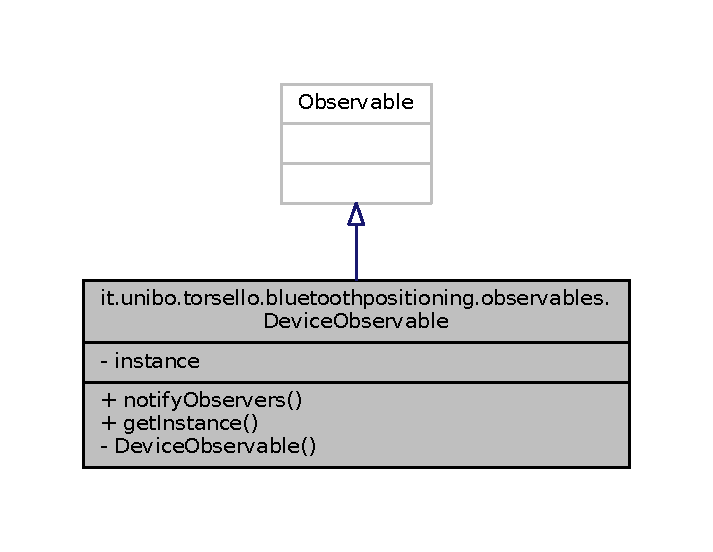
\includegraphics[width=342pt]{classit_1_1unibo_1_1torsello_1_1bluetoothpositioning_1_1observables_1_1DeviceObservable__inherit__graph}
\end{center}
\end{figure}


Diagramma di collaborazione per it.\+unibo.\+torsello.\+bluetoothpositioning.\+observables.\+Device\+Observable\+:
\nopagebreak
\begin{figure}[H]
\begin{center}
\leavevmode
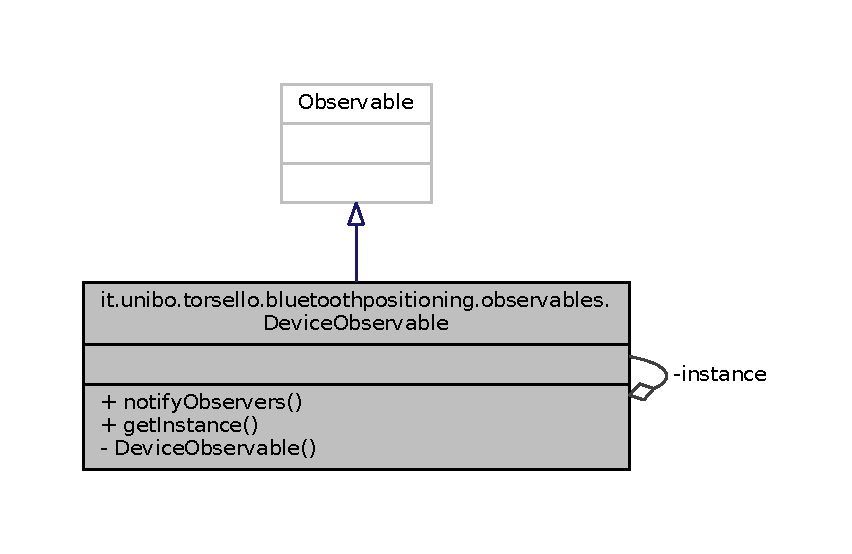
\includegraphics[width=350pt]{classit_1_1unibo_1_1torsello_1_1bluetoothpositioning_1_1observables_1_1DeviceObservable__coll__graph}
\end{center}
\end{figure}
\subsubsection*{Membri pubblici}
\begin{DoxyCompactItemize}
\item 
void \hyperlink{classit_1_1unibo_1_1torsello_1_1bluetoothpositioning_1_1observables_1_1DeviceObservable_aaf183e537e44cbd114c8eb76432da191_aaf183e537e44cbd114c8eb76432da191}{notify\+Observers} (Object data)
\end{DoxyCompactItemize}
\subsubsection*{Membri pubblici statici}
\begin{DoxyCompactItemize}
\item 
static \hyperlink{classit_1_1unibo_1_1torsello_1_1bluetoothpositioning_1_1observables_1_1DeviceObservable}{Device\+Observable} \hyperlink{classit_1_1unibo_1_1torsello_1_1bluetoothpositioning_1_1observables_1_1DeviceObservable_ab16792c5848440646624b2a41553954a_ab16792c5848440646624b2a41553954a}{get\+Instance} ()
\end{DoxyCompactItemize}
\subsubsection*{Membri privati}
\begin{DoxyCompactItemize}
\item 
\hyperlink{classit_1_1unibo_1_1torsello_1_1bluetoothpositioning_1_1observables_1_1DeviceObservable_afd89b681af0ee7708c8d3e830128cd2a_afd89b681af0ee7708c8d3e830128cd2a}{Device\+Observable} ()
\end{DoxyCompactItemize}
\subsubsection*{Attributi privati statici}
\begin{DoxyCompactItemize}
\item 
static \hyperlink{classit_1_1unibo_1_1torsello_1_1bluetoothpositioning_1_1observables_1_1DeviceObservable}{Device\+Observable} \hyperlink{classit_1_1unibo_1_1torsello_1_1bluetoothpositioning_1_1observables_1_1DeviceObservable_a43120f0ae1d6ae6c543219ec42df15e2_a43120f0ae1d6ae6c543219ec42df15e2}{instance} = new \hyperlink{classit_1_1unibo_1_1torsello_1_1bluetoothpositioning_1_1observables_1_1DeviceObservable}{Device\+Observable}()
\end{DoxyCompactItemize}


\subsubsection{Descrizione dettagliata}
Created by Federico Torsello. \href{mailto:federico.torsello@studio.unibo.it}{\tt federico.\+torsello@studio.\+unibo.\+it} 

\subsubsection{Documentazione dei costruttori e dei distruttori}
\hypertarget{classit_1_1unibo_1_1torsello_1_1bluetoothpositioning_1_1observables_1_1DeviceObservable_afd89b681af0ee7708c8d3e830128cd2a_afd89b681af0ee7708c8d3e830128cd2a}{}\label{classit_1_1unibo_1_1torsello_1_1bluetoothpositioning_1_1observables_1_1DeviceObservable_afd89b681af0ee7708c8d3e830128cd2a_afd89b681af0ee7708c8d3e830128cd2a} 
\index{it\+::unibo\+::torsello\+::bluetoothpositioning\+::observables\+::\+Device\+Observable@{it\+::unibo\+::torsello\+::bluetoothpositioning\+::observables\+::\+Device\+Observable}!Device\+Observable@{Device\+Observable}}
\index{Device\+Observable@{Device\+Observable}!it\+::unibo\+::torsello\+::bluetoothpositioning\+::observables\+::\+Device\+Observable@{it\+::unibo\+::torsello\+::bluetoothpositioning\+::observables\+::\+Device\+Observable}}
\paragraph{\texorpdfstring{Device\+Observable()}{DeviceObservable()}}
{\footnotesize\ttfamily it.\+unibo.\+torsello.\+bluetoothpositioning.\+observables.\+Device\+Observable.\+Device\+Observable (\begin{DoxyParamCaption}{ }\end{DoxyParamCaption})\hspace{0.3cm}{\ttfamily [private]}}


\begin{DoxyCode}
13                                \{
14         super();
15     \}
\end{DoxyCode}


\subsubsection{Documentazione delle funzioni membro}
\hypertarget{classit_1_1unibo_1_1torsello_1_1bluetoothpositioning_1_1observables_1_1DeviceObservable_ab16792c5848440646624b2a41553954a_ab16792c5848440646624b2a41553954a}{}\label{classit_1_1unibo_1_1torsello_1_1bluetoothpositioning_1_1observables_1_1DeviceObservable_ab16792c5848440646624b2a41553954a_ab16792c5848440646624b2a41553954a} 
\index{it\+::unibo\+::torsello\+::bluetoothpositioning\+::observables\+::\+Device\+Observable@{it\+::unibo\+::torsello\+::bluetoothpositioning\+::observables\+::\+Device\+Observable}!get\+Instance@{get\+Instance}}
\index{get\+Instance@{get\+Instance}!it\+::unibo\+::torsello\+::bluetoothpositioning\+::observables\+::\+Device\+Observable@{it\+::unibo\+::torsello\+::bluetoothpositioning\+::observables\+::\+Device\+Observable}}
\paragraph{\texorpdfstring{get\+Instance()}{getInstance()}}
{\footnotesize\ttfamily static \hyperlink{classit_1_1unibo_1_1torsello_1_1bluetoothpositioning_1_1observables_1_1DeviceObservable}{Device\+Observable} it.\+unibo.\+torsello.\+bluetoothpositioning.\+observables.\+Device\+Observable.\+get\+Instance (\begin{DoxyParamCaption}{ }\end{DoxyParamCaption})\hspace{0.3cm}{\ttfamily [static]}}


\begin{DoxyCode}
17                                                  \{
18         \textcolor{keywordflow}{return} \hyperlink{classit_1_1unibo_1_1torsello_1_1bluetoothpositioning_1_1observables_1_1DeviceObservable_a43120f0ae1d6ae6c543219ec42df15e2_a43120f0ae1d6ae6c543219ec42df15e2}{instance};
19     \}
\end{DoxyCode}
\hypertarget{classit_1_1unibo_1_1torsello_1_1bluetoothpositioning_1_1observables_1_1DeviceObservable_aaf183e537e44cbd114c8eb76432da191_aaf183e537e44cbd114c8eb76432da191}{}\label{classit_1_1unibo_1_1torsello_1_1bluetoothpositioning_1_1observables_1_1DeviceObservable_aaf183e537e44cbd114c8eb76432da191_aaf183e537e44cbd114c8eb76432da191} 
\index{it\+::unibo\+::torsello\+::bluetoothpositioning\+::observables\+::\+Device\+Observable@{it\+::unibo\+::torsello\+::bluetoothpositioning\+::observables\+::\+Device\+Observable}!notify\+Observers@{notify\+Observers}}
\index{notify\+Observers@{notify\+Observers}!it\+::unibo\+::torsello\+::bluetoothpositioning\+::observables\+::\+Device\+Observable@{it\+::unibo\+::torsello\+::bluetoothpositioning\+::observables\+::\+Device\+Observable}}
\paragraph{\texorpdfstring{notify\+Observers()}{notifyObservers()}}
{\footnotesize\ttfamily void it.\+unibo.\+torsello.\+bluetoothpositioning.\+observables.\+Device\+Observable.\+notify\+Observers (\begin{DoxyParamCaption}\item[{Object}]{data }\end{DoxyParamCaption})}


\begin{DoxyCode}
22                                              \{
23         setChanged();
24         super.notifyObservers(data);
25     \}
\end{DoxyCode}


\subsubsection{Documentazione dei membri dato}
\hypertarget{classit_1_1unibo_1_1torsello_1_1bluetoothpositioning_1_1observables_1_1DeviceObservable_a43120f0ae1d6ae6c543219ec42df15e2_a43120f0ae1d6ae6c543219ec42df15e2}{}\label{classit_1_1unibo_1_1torsello_1_1bluetoothpositioning_1_1observables_1_1DeviceObservable_a43120f0ae1d6ae6c543219ec42df15e2_a43120f0ae1d6ae6c543219ec42df15e2} 
\index{it\+::unibo\+::torsello\+::bluetoothpositioning\+::observables\+::\+Device\+Observable@{it\+::unibo\+::torsello\+::bluetoothpositioning\+::observables\+::\+Device\+Observable}!instance@{instance}}
\index{instance@{instance}!it\+::unibo\+::torsello\+::bluetoothpositioning\+::observables\+::\+Device\+Observable@{it\+::unibo\+::torsello\+::bluetoothpositioning\+::observables\+::\+Device\+Observable}}
\paragraph{\texorpdfstring{instance}{instance}}
{\footnotesize\ttfamily \hyperlink{classit_1_1unibo_1_1torsello_1_1bluetoothpositioning_1_1observables_1_1DeviceObservable}{Device\+Observable} it.\+unibo.\+torsello.\+bluetoothpositioning.\+observables.\+Device\+Observable.\+instance = new \hyperlink{classit_1_1unibo_1_1torsello_1_1bluetoothpositioning_1_1observables_1_1DeviceObservable}{Device\+Observable}()\hspace{0.3cm}{\ttfamily [static]}, {\ttfamily [private]}}



La documentazione per questa classe è stata generata a partire dal seguente file\+:\begin{DoxyCompactItemize}
\item 
\hyperlink{DeviceObservable_8java}{Device\+Observable.\+java}\end{DoxyCompactItemize}

\hypertarget{classit_1_1unibo_1_1torsello_1_1bluetoothpositioning_1_1adapter_1_1DeviceCardViewAdapter_1_1DeviceViewHolder}{}\subsection{Riferimenti per la classe it.\+unibo.\+torsello.\+bluetoothpositioning.\+adapter.\+Device\+Card\+View\+Adapter.\+Device\+View\+Holder}
\label{classit_1_1unibo_1_1torsello_1_1bluetoothpositioning_1_1adapter_1_1DeviceCardViewAdapter_1_1DeviceViewHolder}\index{it.\+unibo.\+torsello.\+bluetoothpositioning.\+adapter.\+Device\+Card\+View\+Adapter.\+Device\+View\+Holder@{it.\+unibo.\+torsello.\+bluetoothpositioning.\+adapter.\+Device\+Card\+View\+Adapter.\+Device\+View\+Holder}}


Diagramma delle classi per it.\+unibo.\+torsello.\+bluetoothpositioning.\+adapter.\+Device\+Card\+View\+Adapter.\+Device\+View\+Holder
\nopagebreak
\begin{figure}[H]
\begin{center}
\leavevmode
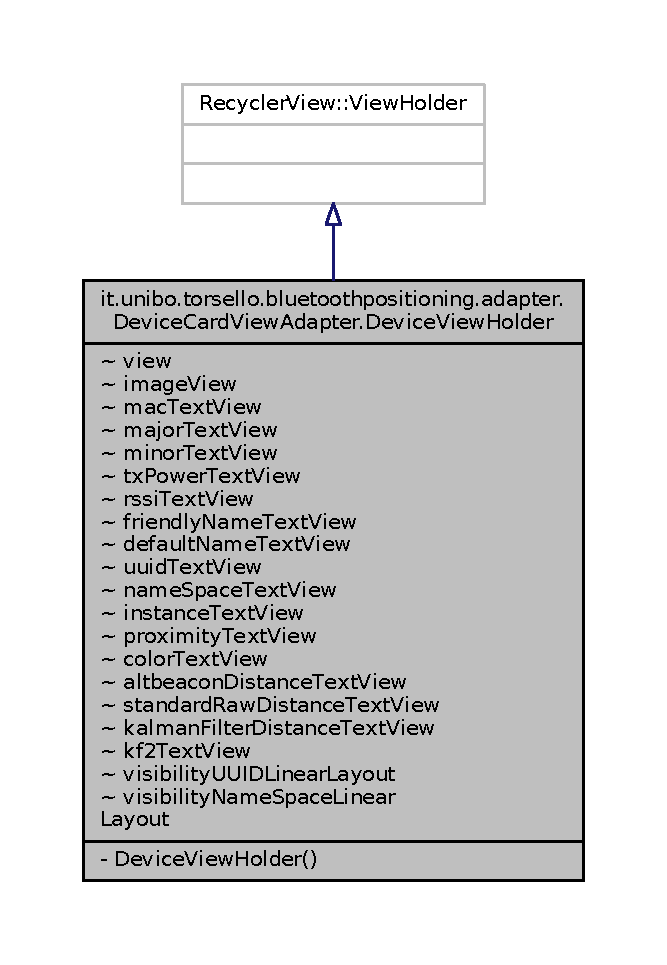
\includegraphics[width=320pt]{classit_1_1unibo_1_1torsello_1_1bluetoothpositioning_1_1adapter_1_1DeviceCardViewAdapter_1_1DeviceViewHolder__inherit__graph}
\end{center}
\end{figure}


Diagramma di collaborazione per it.\+unibo.\+torsello.\+bluetoothpositioning.\+adapter.\+Device\+Card\+View\+Adapter.\+Device\+View\+Holder\+:
\nopagebreak
\begin{figure}[H]
\begin{center}
\leavevmode
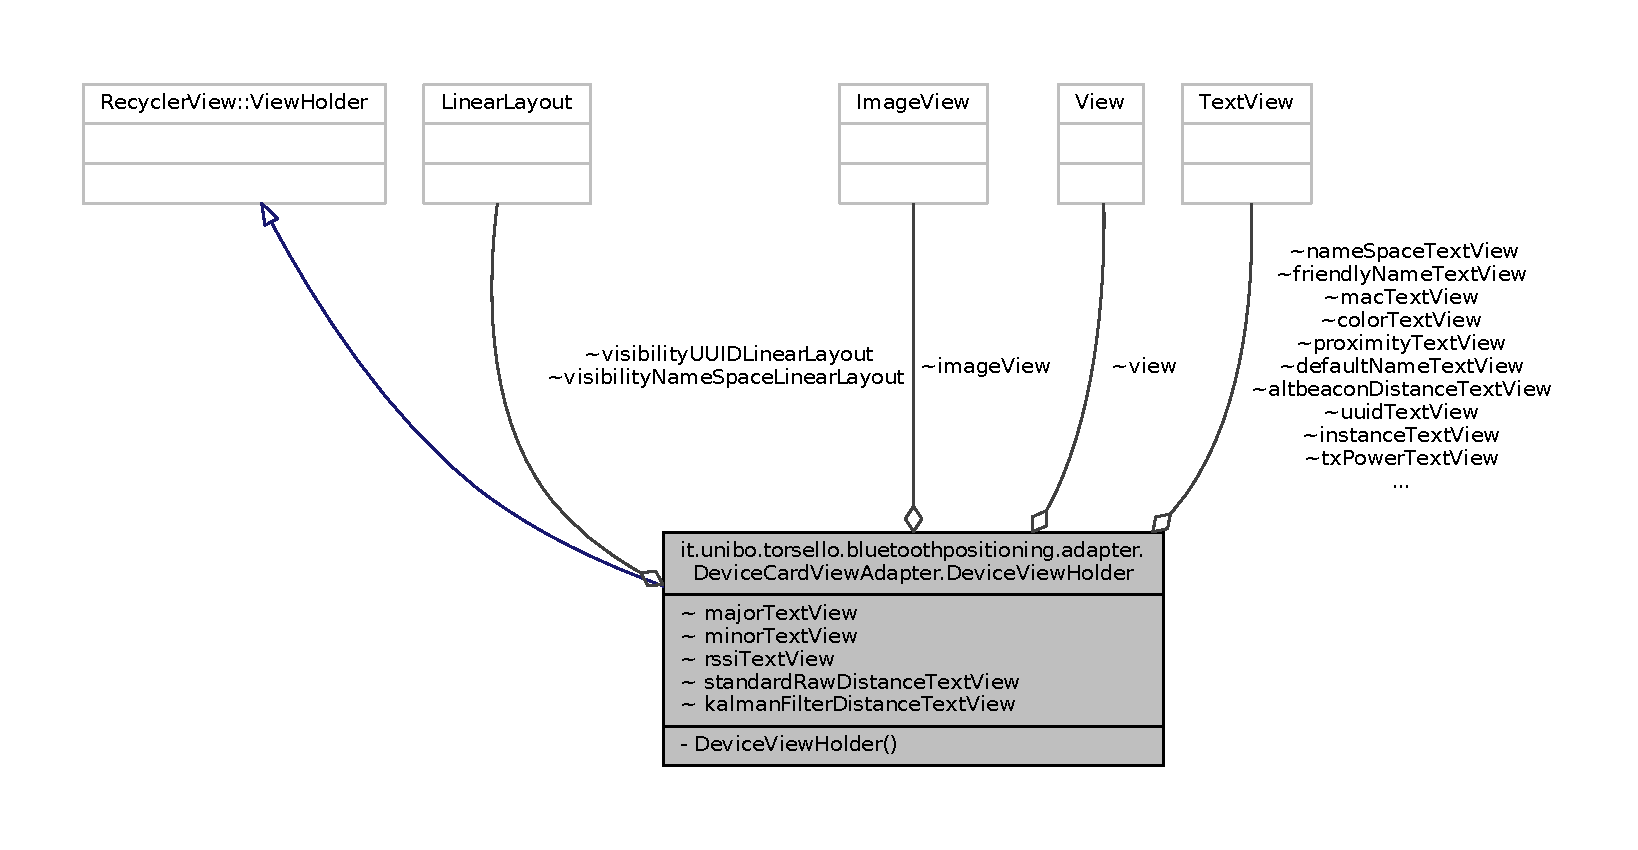
\includegraphics[width=350pt]{classit_1_1unibo_1_1torsello_1_1bluetoothpositioning_1_1adapter_1_1DeviceCardViewAdapter_1_1DeviceViewHolder__coll__graph}
\end{center}
\end{figure}
\subsubsection*{Attributi con visibilità di package}
\begin{DoxyCompactItemize}
\item 
View \hyperlink{classit_1_1unibo_1_1torsello_1_1bluetoothpositioning_1_1adapter_1_1DeviceCardViewAdapter_1_1DeviceViewHolder_a4aa2da965bbcbc091ae913aea1e0a5cd_a4aa2da965bbcbc091ae913aea1e0a5cd}{view}
\item 
Image\+View \hyperlink{classit_1_1unibo_1_1torsello_1_1bluetoothpositioning_1_1adapter_1_1DeviceCardViewAdapter_1_1DeviceViewHolder_a347a5569ea11fee0f721d0853ba1383a_a347a5569ea11fee0f721d0853ba1383a}{image\+View}
\item 
Text\+View \hyperlink{classit_1_1unibo_1_1torsello_1_1bluetoothpositioning_1_1adapter_1_1DeviceCardViewAdapter_1_1DeviceViewHolder_af70da9970d914ec47f1a19c4b46d6fe0_af70da9970d914ec47f1a19c4b46d6fe0}{mac\+Text\+View}
\item 
Text\+View \hyperlink{classit_1_1unibo_1_1torsello_1_1bluetoothpositioning_1_1adapter_1_1DeviceCardViewAdapter_1_1DeviceViewHolder_ab436c91c0fac49199cc1a275ce2911e0_ab436c91c0fac49199cc1a275ce2911e0}{major\+Text\+View}
\item 
Text\+View \hyperlink{classit_1_1unibo_1_1torsello_1_1bluetoothpositioning_1_1adapter_1_1DeviceCardViewAdapter_1_1DeviceViewHolder_ac23ff2b20dcea8f3847023fbe8a6ca00_ac23ff2b20dcea8f3847023fbe8a6ca00}{minor\+Text\+View}
\item 
Text\+View \hyperlink{classit_1_1unibo_1_1torsello_1_1bluetoothpositioning_1_1adapter_1_1DeviceCardViewAdapter_1_1DeviceViewHolder_aefed6d7b85f2616d61a6d5eb3bdc5b42_aefed6d7b85f2616d61a6d5eb3bdc5b42}{tx\+Power\+Text\+View}
\item 
Text\+View \hyperlink{classit_1_1unibo_1_1torsello_1_1bluetoothpositioning_1_1adapter_1_1DeviceCardViewAdapter_1_1DeviceViewHolder_a5a1945d4212a1aff801998aecdb7b89e_a5a1945d4212a1aff801998aecdb7b89e}{rssi\+Text\+View}
\item 
Text\+View \hyperlink{classit_1_1unibo_1_1torsello_1_1bluetoothpositioning_1_1adapter_1_1DeviceCardViewAdapter_1_1DeviceViewHolder_abd00e1fa8a2d2f6c46e6c43d59c43c09_abd00e1fa8a2d2f6c46e6c43d59c43c09}{friendly\+Name\+Text\+View}
\item 
Text\+View \hyperlink{classit_1_1unibo_1_1torsello_1_1bluetoothpositioning_1_1adapter_1_1DeviceCardViewAdapter_1_1DeviceViewHolder_a26c7f741a315cf43fca6570375dca93a_a26c7f741a315cf43fca6570375dca93a}{default\+Name\+Text\+View}
\item 
Text\+View \hyperlink{classit_1_1unibo_1_1torsello_1_1bluetoothpositioning_1_1adapter_1_1DeviceCardViewAdapter_1_1DeviceViewHolder_ac4c704d6332705288b277bddcc922eb3_ac4c704d6332705288b277bddcc922eb3}{uuid\+Text\+View}
\item 
Text\+View \hyperlink{classit_1_1unibo_1_1torsello_1_1bluetoothpositioning_1_1adapter_1_1DeviceCardViewAdapter_1_1DeviceViewHolder_a7c487cde57093a878929990ba61d173c_a7c487cde57093a878929990ba61d173c}{name\+Space\+Text\+View}
\item 
Text\+View \hyperlink{classit_1_1unibo_1_1torsello_1_1bluetoothpositioning_1_1adapter_1_1DeviceCardViewAdapter_1_1DeviceViewHolder_afd46ff4d479b502963dd9630efc9f177_afd46ff4d479b502963dd9630efc9f177}{instance\+Text\+View}
\item 
Text\+View \hyperlink{classit_1_1unibo_1_1torsello_1_1bluetoothpositioning_1_1adapter_1_1DeviceCardViewAdapter_1_1DeviceViewHolder_a1ddd659d463c9b409b4a9df663e0fa05_a1ddd659d463c9b409b4a9df663e0fa05}{proximity\+Text\+View}
\item 
Text\+View \hyperlink{classit_1_1unibo_1_1torsello_1_1bluetoothpositioning_1_1adapter_1_1DeviceCardViewAdapter_1_1DeviceViewHolder_a13b19031bd21f4beee3809d4917429de_a13b19031bd21f4beee3809d4917429de}{color\+Text\+View}
\item 
Text\+View \hyperlink{classit_1_1unibo_1_1torsello_1_1bluetoothpositioning_1_1adapter_1_1DeviceCardViewAdapter_1_1DeviceViewHolder_ac6ec3f5e17e0feda143c7883d6115334_ac6ec3f5e17e0feda143c7883d6115334}{altbeacon\+Distance\+Text\+View}
\item 
Text\+View \hyperlink{classit_1_1unibo_1_1torsello_1_1bluetoothpositioning_1_1adapter_1_1DeviceCardViewAdapter_1_1DeviceViewHolder_a1465eea620da435cda3037fefd715a90_a1465eea620da435cda3037fefd715a90}{standard\+Raw\+Distance\+Text\+View}
\item 
Text\+View \hyperlink{classit_1_1unibo_1_1torsello_1_1bluetoothpositioning_1_1adapter_1_1DeviceCardViewAdapter_1_1DeviceViewHolder_a1e0cad4bb83fa3f733d84ca6decd50c4_a1e0cad4bb83fa3f733d84ca6decd50c4}{kalman\+Filter\+Distance\+Text\+View}
\item 
Linear\+Layout \hyperlink{classit_1_1unibo_1_1torsello_1_1bluetoothpositioning_1_1adapter_1_1DeviceCardViewAdapter_1_1DeviceViewHolder_a72e4e3a233aa8cff4c3fe8e28a156095_a72e4e3a233aa8cff4c3fe8e28a156095}{visibility\+U\+U\+I\+D\+Linear\+Layout}
\item 
Linear\+Layout \hyperlink{classit_1_1unibo_1_1torsello_1_1bluetoothpositioning_1_1adapter_1_1DeviceCardViewAdapter_1_1DeviceViewHolder_aa3b69bc26e552aef6c18acb40e991d27_aa3b69bc26e552aef6c18acb40e991d27}{visibility\+Name\+Space\+Linear\+Layout}
\end{DoxyCompactItemize}
\subsubsection*{Membri privati}
\begin{DoxyCompactItemize}
\item 
\hyperlink{classit_1_1unibo_1_1torsello_1_1bluetoothpositioning_1_1adapter_1_1DeviceCardViewAdapter_1_1DeviceViewHolder_a75016d2a0df1fc991a5a6aed86b776d2_a75016d2a0df1fc991a5a6aed86b776d2}{Device\+View\+Holder} (View \hyperlink{classit_1_1unibo_1_1torsello_1_1bluetoothpositioning_1_1adapter_1_1DeviceCardViewAdapter_1_1DeviceViewHolder_a4aa2da965bbcbc091ae913aea1e0a5cd_a4aa2da965bbcbc091ae913aea1e0a5cd}{view})
\end{DoxyCompactItemize}


\subsubsection{Documentazione dei costruttori e dei distruttori}
\hypertarget{classit_1_1unibo_1_1torsello_1_1bluetoothpositioning_1_1adapter_1_1DeviceCardViewAdapter_1_1DeviceViewHolder_a75016d2a0df1fc991a5a6aed86b776d2_a75016d2a0df1fc991a5a6aed86b776d2}{}\label{classit_1_1unibo_1_1torsello_1_1bluetoothpositioning_1_1adapter_1_1DeviceCardViewAdapter_1_1DeviceViewHolder_a75016d2a0df1fc991a5a6aed86b776d2_a75016d2a0df1fc991a5a6aed86b776d2} 
\index{it\+::unibo\+::torsello\+::bluetoothpositioning\+::adapter\+::\+Device\+Card\+View\+Adapter\+::\+Device\+View\+Holder@{it\+::unibo\+::torsello\+::bluetoothpositioning\+::adapter\+::\+Device\+Card\+View\+Adapter\+::\+Device\+View\+Holder}!Device\+View\+Holder@{Device\+View\+Holder}}
\index{Device\+View\+Holder@{Device\+View\+Holder}!it\+::unibo\+::torsello\+::bluetoothpositioning\+::adapter\+::\+Device\+Card\+View\+Adapter\+::\+Device\+View\+Holder@{it\+::unibo\+::torsello\+::bluetoothpositioning\+::adapter\+::\+Device\+Card\+View\+Adapter\+::\+Device\+View\+Holder}}
\paragraph{\texorpdfstring{Device\+View\+Holder()}{DeviceViewHolder()}}
{\footnotesize\ttfamily it.\+unibo.\+torsello.\+bluetoothpositioning.\+adapter.\+Device\+Card\+View\+Adapter.\+Device\+View\+Holder.\+Device\+View\+Holder (\begin{DoxyParamCaption}\item[{View}]{view }\end{DoxyParamCaption})\hspace{0.3cm}{\ttfamily [private]}}


\begin{DoxyCode}
250                                             \{
251 
252             super(\hyperlink{classit_1_1unibo_1_1torsello_1_1bluetoothpositioning_1_1adapter_1_1DeviceCardViewAdapter_1_1DeviceViewHolder_a4aa2da965bbcbc091ae913aea1e0a5cd_a4aa2da965bbcbc091ae913aea1e0a5cd}{view});
253             this.\hyperlink{classit_1_1unibo_1_1torsello_1_1bluetoothpositioning_1_1adapter_1_1DeviceCardViewAdapter_1_1DeviceViewHolder_a4aa2da965bbcbc091ae913aea1e0a5cd_a4aa2da965bbcbc091ae913aea1e0a5cd}{view} = \hyperlink{classit_1_1unibo_1_1torsello_1_1bluetoothpositioning_1_1adapter_1_1DeviceCardViewAdapter_1_1DeviceViewHolder_a4aa2da965bbcbc091ae913aea1e0a5cd_a4aa2da965bbcbc091ae913aea1e0a5cd}{view};
254             \hyperlink{classit_1_1unibo_1_1torsello_1_1bluetoothpositioning_1_1adapter_1_1DeviceCardViewAdapter_1_1DeviceViewHolder_a347a5569ea11fee0f721d0853ba1383a_a347a5569ea11fee0f721d0853ba1383a}{imageView} = (ImageView) \hyperlink{classit_1_1unibo_1_1torsello_1_1bluetoothpositioning_1_1adapter_1_1DeviceCardViewAdapter_1_1DeviceViewHolder_a4aa2da965bbcbc091ae913aea1e0a5cd_a4aa2da965bbcbc091ae913aea1e0a5cd}{view}.findViewById(R.id.imageBeacon);
255             \hyperlink{classit_1_1unibo_1_1torsello_1_1bluetoothpositioning_1_1adapter_1_1DeviceCardViewAdapter_1_1DeviceViewHolder_a26c7f741a315cf43fca6570375dca93a_a26c7f741a315cf43fca6570375dca93a}{defaultNameTextView} = (TextView) \hyperlink{classit_1_1unibo_1_1torsello_1_1bluetoothpositioning_1_1adapter_1_1DeviceCardViewAdapter_1_1DeviceViewHolder_a4aa2da965bbcbc091ae913aea1e0a5cd_a4aa2da965bbcbc091ae913aea1e0a5cd}{view}.findViewById(R.id.
      value\_default\_name);
256             \hyperlink{classit_1_1unibo_1_1torsello_1_1bluetoothpositioning_1_1adapter_1_1DeviceCardViewAdapter_1_1DeviceViewHolder_abd00e1fa8a2d2f6c46e6c43d59c43c09_abd00e1fa8a2d2f6c46e6c43d59c43c09}{friendlyNameTextView} = (TextView) \hyperlink{classit_1_1unibo_1_1torsello_1_1bluetoothpositioning_1_1adapter_1_1DeviceCardViewAdapter_1_1DeviceViewHolder_a4aa2da965bbcbc091ae913aea1e0a5cd_a4aa2da965bbcbc091ae913aea1e0a5cd}{view}.findViewById(R.id.
      value\_friendly\_name);
257             \hyperlink{classit_1_1unibo_1_1torsello_1_1bluetoothpositioning_1_1adapter_1_1DeviceCardViewAdapter_1_1DeviceViewHolder_af70da9970d914ec47f1a19c4b46d6fe0_af70da9970d914ec47f1a19c4b46d6fe0}{macTextView} = (TextView) \hyperlink{classit_1_1unibo_1_1torsello_1_1bluetoothpositioning_1_1adapter_1_1DeviceCardViewAdapter_1_1DeviceViewHolder_a4aa2da965bbcbc091ae913aea1e0a5cd_a4aa2da965bbcbc091ae913aea1e0a5cd}{view}.findViewById(R.id.value\_mac\_address);
258             \hyperlink{classit_1_1unibo_1_1torsello_1_1bluetoothpositioning_1_1adapter_1_1DeviceCardViewAdapter_1_1DeviceViewHolder_ab436c91c0fac49199cc1a275ce2911e0_ab436c91c0fac49199cc1a275ce2911e0}{majorTextView} = (TextView) \hyperlink{classit_1_1unibo_1_1torsello_1_1bluetoothpositioning_1_1adapter_1_1DeviceCardViewAdapter_1_1DeviceViewHolder_a4aa2da965bbcbc091ae913aea1e0a5cd_a4aa2da965bbcbc091ae913aea1e0a5cd}{view}.findViewById(R.id.value\_major);
259             \hyperlink{classit_1_1unibo_1_1torsello_1_1bluetoothpositioning_1_1adapter_1_1DeviceCardViewAdapter_1_1DeviceViewHolder_ac23ff2b20dcea8f3847023fbe8a6ca00_ac23ff2b20dcea8f3847023fbe8a6ca00}{minorTextView} = (TextView) \hyperlink{classit_1_1unibo_1_1torsello_1_1bluetoothpositioning_1_1adapter_1_1DeviceCardViewAdapter_1_1DeviceViewHolder_a4aa2da965bbcbc091ae913aea1e0a5cd_a4aa2da965bbcbc091ae913aea1e0a5cd}{view}.findViewById(R.id.value\_minor);
260             \hyperlink{classit_1_1unibo_1_1torsello_1_1bluetoothpositioning_1_1adapter_1_1DeviceCardViewAdapter_1_1DeviceViewHolder_aefed6d7b85f2616d61a6d5eb3bdc5b42_aefed6d7b85f2616d61a6d5eb3bdc5b42}{txPowerTextView} = (TextView) \hyperlink{classit_1_1unibo_1_1torsello_1_1bluetoothpositioning_1_1adapter_1_1DeviceCardViewAdapter_1_1DeviceViewHolder_a4aa2da965bbcbc091ae913aea1e0a5cd_a4aa2da965bbcbc091ae913aea1e0a5cd}{view}.findViewById(R.id.value\_power);
261             \hyperlink{classit_1_1unibo_1_1torsello_1_1bluetoothpositioning_1_1adapter_1_1DeviceCardViewAdapter_1_1DeviceViewHolder_a5a1945d4212a1aff801998aecdb7b89e_a5a1945d4212a1aff801998aecdb7b89e}{rssiTextView} = (TextView) \hyperlink{classit_1_1unibo_1_1torsello_1_1bluetoothpositioning_1_1adapter_1_1DeviceCardViewAdapter_1_1DeviceViewHolder_a4aa2da965bbcbc091ae913aea1e0a5cd_a4aa2da965bbcbc091ae913aea1e0a5cd}{view}.findViewById(R.id.value\_rssi);
262             \hyperlink{classit_1_1unibo_1_1torsello_1_1bluetoothpositioning_1_1adapter_1_1DeviceCardViewAdapter_1_1DeviceViewHolder_ac4c704d6332705288b277bddcc922eb3_ac4c704d6332705288b277bddcc922eb3}{uuidTextView} = (TextView) \hyperlink{classit_1_1unibo_1_1torsello_1_1bluetoothpositioning_1_1adapter_1_1DeviceCardViewAdapter_1_1DeviceViewHolder_a4aa2da965bbcbc091ae913aea1e0a5cd_a4aa2da965bbcbc091ae913aea1e0a5cd}{view}.findViewById(R.id.value\_uuid);
263             \hyperlink{classit_1_1unibo_1_1torsello_1_1bluetoothpositioning_1_1adapter_1_1DeviceCardViewAdapter_1_1DeviceViewHolder_a7c487cde57093a878929990ba61d173c_a7c487cde57093a878929990ba61d173c}{nameSpaceTextView} = (TextView) \hyperlink{classit_1_1unibo_1_1torsello_1_1bluetoothpositioning_1_1adapter_1_1DeviceCardViewAdapter_1_1DeviceViewHolder_a4aa2da965bbcbc091ae913aea1e0a5cd_a4aa2da965bbcbc091ae913aea1e0a5cd}{view}.findViewById(R.id.value\_name\_space);
264             \hyperlink{classit_1_1unibo_1_1torsello_1_1bluetoothpositioning_1_1adapter_1_1DeviceCardViewAdapter_1_1DeviceViewHolder_a1ddd659d463c9b409b4a9df663e0fa05_a1ddd659d463c9b409b4a9df663e0fa05}{proximityTextView} = (TextView) \hyperlink{classit_1_1unibo_1_1torsello_1_1bluetoothpositioning_1_1adapter_1_1DeviceCardViewAdapter_1_1DeviceViewHolder_a4aa2da965bbcbc091ae913aea1e0a5cd_a4aa2da965bbcbc091ae913aea1e0a5cd}{view}.findViewById(R.id.value\_proximity);
265             \hyperlink{classit_1_1unibo_1_1torsello_1_1bluetoothpositioning_1_1adapter_1_1DeviceCardViewAdapter_1_1DeviceViewHolder_afd46ff4d479b502963dd9630efc9f177_afd46ff4d479b502963dd9630efc9f177}{instanceTextView} = (TextView) \hyperlink{classit_1_1unibo_1_1torsello_1_1bluetoothpositioning_1_1adapter_1_1DeviceCardViewAdapter_1_1DeviceViewHolder_a4aa2da965bbcbc091ae913aea1e0a5cd_a4aa2da965bbcbc091ae913aea1e0a5cd}{view}.findViewById(R.id.value\_instance);
266             \hyperlink{classit_1_1unibo_1_1torsello_1_1bluetoothpositioning_1_1adapter_1_1DeviceCardViewAdapter_1_1DeviceViewHolder_a13b19031bd21f4beee3809d4917429de_a13b19031bd21f4beee3809d4917429de}{colorTextView} = (TextView) \hyperlink{classit_1_1unibo_1_1torsello_1_1bluetoothpositioning_1_1adapter_1_1DeviceCardViewAdapter_1_1DeviceViewHolder_a4aa2da965bbcbc091ae913aea1e0a5cd_a4aa2da965bbcbc091ae913aea1e0a5cd}{view}.findViewById(R.id.value\_color);
267 
268             \hyperlink{classit_1_1unibo_1_1torsello_1_1bluetoothpositioning_1_1adapter_1_1DeviceCardViewAdapter_1_1DeviceViewHolder_ac6ec3f5e17e0feda143c7883d6115334_ac6ec3f5e17e0feda143c7883d6115334}{altbeaconDistanceTextView} = (TextView) \hyperlink{classit_1_1unibo_1_1torsello_1_1bluetoothpositioning_1_1adapter_1_1DeviceCardViewAdapter_1_1DeviceViewHolder_a4aa2da965bbcbc091ae913aea1e0a5cd_a4aa2da965bbcbc091ae913aea1e0a5cd}{view}.findViewById(R.id.
      value\_altbeacon\_distance);
269             \hyperlink{classit_1_1unibo_1_1torsello_1_1bluetoothpositioning_1_1adapter_1_1DeviceCardViewAdapter_1_1DeviceViewHolder_a1e0cad4bb83fa3f733d84ca6decd50c4_a1e0cad4bb83fa3f733d84ca6decd50c4}{kalmanFilterDistanceTextView} = (TextView) 
      \hyperlink{classit_1_1unibo_1_1torsello_1_1bluetoothpositioning_1_1adapter_1_1DeviceCardViewAdapter_1_1DeviceViewHolder_a4aa2da965bbcbc091ae913aea1e0a5cd_a4aa2da965bbcbc091ae913aea1e0a5cd}{view}.findViewById(R.id.value\_kalman\_filter\_distance);
270             \hyperlink{classit_1_1unibo_1_1torsello_1_1bluetoothpositioning_1_1adapter_1_1DeviceCardViewAdapter_1_1DeviceViewHolder_a1465eea620da435cda3037fefd715a90_a1465eea620da435cda3037fefd715a90}{standardRawDistanceTextView} = (TextView) 
      \hyperlink{classit_1_1unibo_1_1torsello_1_1bluetoothpositioning_1_1adapter_1_1DeviceCardViewAdapter_1_1DeviceViewHolder_a4aa2da965bbcbc091ae913aea1e0a5cd_a4aa2da965bbcbc091ae913aea1e0a5cd}{view}.findViewById(R.id.value\_standard\_raw\_distance);
271 
272             \hyperlink{classit_1_1unibo_1_1torsello_1_1bluetoothpositioning_1_1adapter_1_1DeviceCardViewAdapter_1_1DeviceViewHolder_a72e4e3a233aa8cff4c3fe8e28a156095_a72e4e3a233aa8cff4c3fe8e28a156095}{visibilityUUIDLinearLayout} = (LinearLayout) 
      \hyperlink{classit_1_1unibo_1_1torsello_1_1bluetoothpositioning_1_1adapter_1_1DeviceCardViewAdapter_1_1DeviceViewHolder_a4aa2da965bbcbc091ae913aea1e0a5cd_a4aa2da965bbcbc091ae913aea1e0a5cd}{view}.findViewById(R.id.visibility\_uuid\_minor\_major\_nmb);
273             \hyperlink{classit_1_1unibo_1_1torsello_1_1bluetoothpositioning_1_1adapter_1_1DeviceCardViewAdapter_1_1DeviceViewHolder_aa3b69bc26e552aef6c18acb40e991d27_aa3b69bc26e552aef6c18acb40e991d27}{visibilityNameSpaceLinearLayout} = (LinearLayout) 
      \hyperlink{classit_1_1unibo_1_1torsello_1_1bluetoothpositioning_1_1adapter_1_1DeviceCardViewAdapter_1_1DeviceViewHolder_a4aa2da965bbcbc091ae913aea1e0a5cd_a4aa2da965bbcbc091ae913aea1e0a5cd}{view}.findViewById(R.id.visibilityNameSpace\_Instance);
274         \}
\end{DoxyCode}


\subsubsection{Documentazione dei membri dato}
\hypertarget{classit_1_1unibo_1_1torsello_1_1bluetoothpositioning_1_1adapter_1_1DeviceCardViewAdapter_1_1DeviceViewHolder_ac6ec3f5e17e0feda143c7883d6115334_ac6ec3f5e17e0feda143c7883d6115334}{}\label{classit_1_1unibo_1_1torsello_1_1bluetoothpositioning_1_1adapter_1_1DeviceCardViewAdapter_1_1DeviceViewHolder_ac6ec3f5e17e0feda143c7883d6115334_ac6ec3f5e17e0feda143c7883d6115334} 
\index{it\+::unibo\+::torsello\+::bluetoothpositioning\+::adapter\+::\+Device\+Card\+View\+Adapter\+::\+Device\+View\+Holder@{it\+::unibo\+::torsello\+::bluetoothpositioning\+::adapter\+::\+Device\+Card\+View\+Adapter\+::\+Device\+View\+Holder}!altbeacon\+Distance\+Text\+View@{altbeacon\+Distance\+Text\+View}}
\index{altbeacon\+Distance\+Text\+View@{altbeacon\+Distance\+Text\+View}!it\+::unibo\+::torsello\+::bluetoothpositioning\+::adapter\+::\+Device\+Card\+View\+Adapter\+::\+Device\+View\+Holder@{it\+::unibo\+::torsello\+::bluetoothpositioning\+::adapter\+::\+Device\+Card\+View\+Adapter\+::\+Device\+View\+Holder}}
\paragraph{\texorpdfstring{altbeacon\+Distance\+Text\+View}{altbeaconDistanceTextView}}
{\footnotesize\ttfamily Text\+View it.\+unibo.\+torsello.\+bluetoothpositioning.\+adapter.\+Device\+Card\+View\+Adapter.\+Device\+View\+Holder.\+altbeacon\+Distance\+Text\+View\hspace{0.3cm}{\ttfamily [package]}}

\hypertarget{classit_1_1unibo_1_1torsello_1_1bluetoothpositioning_1_1adapter_1_1DeviceCardViewAdapter_1_1DeviceViewHolder_a13b19031bd21f4beee3809d4917429de_a13b19031bd21f4beee3809d4917429de}{}\label{classit_1_1unibo_1_1torsello_1_1bluetoothpositioning_1_1adapter_1_1DeviceCardViewAdapter_1_1DeviceViewHolder_a13b19031bd21f4beee3809d4917429de_a13b19031bd21f4beee3809d4917429de} 
\index{it\+::unibo\+::torsello\+::bluetoothpositioning\+::adapter\+::\+Device\+Card\+View\+Adapter\+::\+Device\+View\+Holder@{it\+::unibo\+::torsello\+::bluetoothpositioning\+::adapter\+::\+Device\+Card\+View\+Adapter\+::\+Device\+View\+Holder}!color\+Text\+View@{color\+Text\+View}}
\index{color\+Text\+View@{color\+Text\+View}!it\+::unibo\+::torsello\+::bluetoothpositioning\+::adapter\+::\+Device\+Card\+View\+Adapter\+::\+Device\+View\+Holder@{it\+::unibo\+::torsello\+::bluetoothpositioning\+::adapter\+::\+Device\+Card\+View\+Adapter\+::\+Device\+View\+Holder}}
\paragraph{\texorpdfstring{color\+Text\+View}{colorTextView}}
{\footnotesize\ttfamily Text\+View it.\+unibo.\+torsello.\+bluetoothpositioning.\+adapter.\+Device\+Card\+View\+Adapter.\+Device\+View\+Holder.\+color\+Text\+View\hspace{0.3cm}{\ttfamily [package]}}

\hypertarget{classit_1_1unibo_1_1torsello_1_1bluetoothpositioning_1_1adapter_1_1DeviceCardViewAdapter_1_1DeviceViewHolder_a26c7f741a315cf43fca6570375dca93a_a26c7f741a315cf43fca6570375dca93a}{}\label{classit_1_1unibo_1_1torsello_1_1bluetoothpositioning_1_1adapter_1_1DeviceCardViewAdapter_1_1DeviceViewHolder_a26c7f741a315cf43fca6570375dca93a_a26c7f741a315cf43fca6570375dca93a} 
\index{it\+::unibo\+::torsello\+::bluetoothpositioning\+::adapter\+::\+Device\+Card\+View\+Adapter\+::\+Device\+View\+Holder@{it\+::unibo\+::torsello\+::bluetoothpositioning\+::adapter\+::\+Device\+Card\+View\+Adapter\+::\+Device\+View\+Holder}!default\+Name\+Text\+View@{default\+Name\+Text\+View}}
\index{default\+Name\+Text\+View@{default\+Name\+Text\+View}!it\+::unibo\+::torsello\+::bluetoothpositioning\+::adapter\+::\+Device\+Card\+View\+Adapter\+::\+Device\+View\+Holder@{it\+::unibo\+::torsello\+::bluetoothpositioning\+::adapter\+::\+Device\+Card\+View\+Adapter\+::\+Device\+View\+Holder}}
\paragraph{\texorpdfstring{default\+Name\+Text\+View}{defaultNameTextView}}
{\footnotesize\ttfamily Text\+View it.\+unibo.\+torsello.\+bluetoothpositioning.\+adapter.\+Device\+Card\+View\+Adapter.\+Device\+View\+Holder.\+default\+Name\+Text\+View\hspace{0.3cm}{\ttfamily [package]}}

\hypertarget{classit_1_1unibo_1_1torsello_1_1bluetoothpositioning_1_1adapter_1_1DeviceCardViewAdapter_1_1DeviceViewHolder_abd00e1fa8a2d2f6c46e6c43d59c43c09_abd00e1fa8a2d2f6c46e6c43d59c43c09}{}\label{classit_1_1unibo_1_1torsello_1_1bluetoothpositioning_1_1adapter_1_1DeviceCardViewAdapter_1_1DeviceViewHolder_abd00e1fa8a2d2f6c46e6c43d59c43c09_abd00e1fa8a2d2f6c46e6c43d59c43c09} 
\index{it\+::unibo\+::torsello\+::bluetoothpositioning\+::adapter\+::\+Device\+Card\+View\+Adapter\+::\+Device\+View\+Holder@{it\+::unibo\+::torsello\+::bluetoothpositioning\+::adapter\+::\+Device\+Card\+View\+Adapter\+::\+Device\+View\+Holder}!friendly\+Name\+Text\+View@{friendly\+Name\+Text\+View}}
\index{friendly\+Name\+Text\+View@{friendly\+Name\+Text\+View}!it\+::unibo\+::torsello\+::bluetoothpositioning\+::adapter\+::\+Device\+Card\+View\+Adapter\+::\+Device\+View\+Holder@{it\+::unibo\+::torsello\+::bluetoothpositioning\+::adapter\+::\+Device\+Card\+View\+Adapter\+::\+Device\+View\+Holder}}
\paragraph{\texorpdfstring{friendly\+Name\+Text\+View}{friendlyNameTextView}}
{\footnotesize\ttfamily Text\+View it.\+unibo.\+torsello.\+bluetoothpositioning.\+adapter.\+Device\+Card\+View\+Adapter.\+Device\+View\+Holder.\+friendly\+Name\+Text\+View\hspace{0.3cm}{\ttfamily [package]}}

\hypertarget{classit_1_1unibo_1_1torsello_1_1bluetoothpositioning_1_1adapter_1_1DeviceCardViewAdapter_1_1DeviceViewHolder_a347a5569ea11fee0f721d0853ba1383a_a347a5569ea11fee0f721d0853ba1383a}{}\label{classit_1_1unibo_1_1torsello_1_1bluetoothpositioning_1_1adapter_1_1DeviceCardViewAdapter_1_1DeviceViewHolder_a347a5569ea11fee0f721d0853ba1383a_a347a5569ea11fee0f721d0853ba1383a} 
\index{it\+::unibo\+::torsello\+::bluetoothpositioning\+::adapter\+::\+Device\+Card\+View\+Adapter\+::\+Device\+View\+Holder@{it\+::unibo\+::torsello\+::bluetoothpositioning\+::adapter\+::\+Device\+Card\+View\+Adapter\+::\+Device\+View\+Holder}!image\+View@{image\+View}}
\index{image\+View@{image\+View}!it\+::unibo\+::torsello\+::bluetoothpositioning\+::adapter\+::\+Device\+Card\+View\+Adapter\+::\+Device\+View\+Holder@{it\+::unibo\+::torsello\+::bluetoothpositioning\+::adapter\+::\+Device\+Card\+View\+Adapter\+::\+Device\+View\+Holder}}
\paragraph{\texorpdfstring{image\+View}{imageView}}
{\footnotesize\ttfamily Image\+View it.\+unibo.\+torsello.\+bluetoothpositioning.\+adapter.\+Device\+Card\+View\+Adapter.\+Device\+View\+Holder.\+image\+View\hspace{0.3cm}{\ttfamily [package]}}

\hypertarget{classit_1_1unibo_1_1torsello_1_1bluetoothpositioning_1_1adapter_1_1DeviceCardViewAdapter_1_1DeviceViewHolder_afd46ff4d479b502963dd9630efc9f177_afd46ff4d479b502963dd9630efc9f177}{}\label{classit_1_1unibo_1_1torsello_1_1bluetoothpositioning_1_1adapter_1_1DeviceCardViewAdapter_1_1DeviceViewHolder_afd46ff4d479b502963dd9630efc9f177_afd46ff4d479b502963dd9630efc9f177} 
\index{it\+::unibo\+::torsello\+::bluetoothpositioning\+::adapter\+::\+Device\+Card\+View\+Adapter\+::\+Device\+View\+Holder@{it\+::unibo\+::torsello\+::bluetoothpositioning\+::adapter\+::\+Device\+Card\+View\+Adapter\+::\+Device\+View\+Holder}!instance\+Text\+View@{instance\+Text\+View}}
\index{instance\+Text\+View@{instance\+Text\+View}!it\+::unibo\+::torsello\+::bluetoothpositioning\+::adapter\+::\+Device\+Card\+View\+Adapter\+::\+Device\+View\+Holder@{it\+::unibo\+::torsello\+::bluetoothpositioning\+::adapter\+::\+Device\+Card\+View\+Adapter\+::\+Device\+View\+Holder}}
\paragraph{\texorpdfstring{instance\+Text\+View}{instanceTextView}}
{\footnotesize\ttfamily Text\+View it.\+unibo.\+torsello.\+bluetoothpositioning.\+adapter.\+Device\+Card\+View\+Adapter.\+Device\+View\+Holder.\+instance\+Text\+View\hspace{0.3cm}{\ttfamily [package]}}

\hypertarget{classit_1_1unibo_1_1torsello_1_1bluetoothpositioning_1_1adapter_1_1DeviceCardViewAdapter_1_1DeviceViewHolder_a1e0cad4bb83fa3f733d84ca6decd50c4_a1e0cad4bb83fa3f733d84ca6decd50c4}{}\label{classit_1_1unibo_1_1torsello_1_1bluetoothpositioning_1_1adapter_1_1DeviceCardViewAdapter_1_1DeviceViewHolder_a1e0cad4bb83fa3f733d84ca6decd50c4_a1e0cad4bb83fa3f733d84ca6decd50c4} 
\index{it\+::unibo\+::torsello\+::bluetoothpositioning\+::adapter\+::\+Device\+Card\+View\+Adapter\+::\+Device\+View\+Holder@{it\+::unibo\+::torsello\+::bluetoothpositioning\+::adapter\+::\+Device\+Card\+View\+Adapter\+::\+Device\+View\+Holder}!kalman\+Filter\+Distance\+Text\+View@{kalman\+Filter\+Distance\+Text\+View}}
\index{kalman\+Filter\+Distance\+Text\+View@{kalman\+Filter\+Distance\+Text\+View}!it\+::unibo\+::torsello\+::bluetoothpositioning\+::adapter\+::\+Device\+Card\+View\+Adapter\+::\+Device\+View\+Holder@{it\+::unibo\+::torsello\+::bluetoothpositioning\+::adapter\+::\+Device\+Card\+View\+Adapter\+::\+Device\+View\+Holder}}
\paragraph{\texorpdfstring{kalman\+Filter\+Distance\+Text\+View}{kalmanFilterDistanceTextView}}
{\footnotesize\ttfamily Text\+View it.\+unibo.\+torsello.\+bluetoothpositioning.\+adapter.\+Device\+Card\+View\+Adapter.\+Device\+View\+Holder.\+kalman\+Filter\+Distance\+Text\+View\hspace{0.3cm}{\ttfamily [package]}}

\hypertarget{classit_1_1unibo_1_1torsello_1_1bluetoothpositioning_1_1adapter_1_1DeviceCardViewAdapter_1_1DeviceViewHolder_af70da9970d914ec47f1a19c4b46d6fe0_af70da9970d914ec47f1a19c4b46d6fe0}{}\label{classit_1_1unibo_1_1torsello_1_1bluetoothpositioning_1_1adapter_1_1DeviceCardViewAdapter_1_1DeviceViewHolder_af70da9970d914ec47f1a19c4b46d6fe0_af70da9970d914ec47f1a19c4b46d6fe0} 
\index{it\+::unibo\+::torsello\+::bluetoothpositioning\+::adapter\+::\+Device\+Card\+View\+Adapter\+::\+Device\+View\+Holder@{it\+::unibo\+::torsello\+::bluetoothpositioning\+::adapter\+::\+Device\+Card\+View\+Adapter\+::\+Device\+View\+Holder}!mac\+Text\+View@{mac\+Text\+View}}
\index{mac\+Text\+View@{mac\+Text\+View}!it\+::unibo\+::torsello\+::bluetoothpositioning\+::adapter\+::\+Device\+Card\+View\+Adapter\+::\+Device\+View\+Holder@{it\+::unibo\+::torsello\+::bluetoothpositioning\+::adapter\+::\+Device\+Card\+View\+Adapter\+::\+Device\+View\+Holder}}
\paragraph{\texorpdfstring{mac\+Text\+View}{macTextView}}
{\footnotesize\ttfamily Text\+View it.\+unibo.\+torsello.\+bluetoothpositioning.\+adapter.\+Device\+Card\+View\+Adapter.\+Device\+View\+Holder.\+mac\+Text\+View\hspace{0.3cm}{\ttfamily [package]}}

\hypertarget{classit_1_1unibo_1_1torsello_1_1bluetoothpositioning_1_1adapter_1_1DeviceCardViewAdapter_1_1DeviceViewHolder_ab436c91c0fac49199cc1a275ce2911e0_ab436c91c0fac49199cc1a275ce2911e0}{}\label{classit_1_1unibo_1_1torsello_1_1bluetoothpositioning_1_1adapter_1_1DeviceCardViewAdapter_1_1DeviceViewHolder_ab436c91c0fac49199cc1a275ce2911e0_ab436c91c0fac49199cc1a275ce2911e0} 
\index{it\+::unibo\+::torsello\+::bluetoothpositioning\+::adapter\+::\+Device\+Card\+View\+Adapter\+::\+Device\+View\+Holder@{it\+::unibo\+::torsello\+::bluetoothpositioning\+::adapter\+::\+Device\+Card\+View\+Adapter\+::\+Device\+View\+Holder}!major\+Text\+View@{major\+Text\+View}}
\index{major\+Text\+View@{major\+Text\+View}!it\+::unibo\+::torsello\+::bluetoothpositioning\+::adapter\+::\+Device\+Card\+View\+Adapter\+::\+Device\+View\+Holder@{it\+::unibo\+::torsello\+::bluetoothpositioning\+::adapter\+::\+Device\+Card\+View\+Adapter\+::\+Device\+View\+Holder}}
\paragraph{\texorpdfstring{major\+Text\+View}{majorTextView}}
{\footnotesize\ttfamily Text\+View it.\+unibo.\+torsello.\+bluetoothpositioning.\+adapter.\+Device\+Card\+View\+Adapter.\+Device\+View\+Holder.\+major\+Text\+View\hspace{0.3cm}{\ttfamily [package]}}

\hypertarget{classit_1_1unibo_1_1torsello_1_1bluetoothpositioning_1_1adapter_1_1DeviceCardViewAdapter_1_1DeviceViewHolder_ac23ff2b20dcea8f3847023fbe8a6ca00_ac23ff2b20dcea8f3847023fbe8a6ca00}{}\label{classit_1_1unibo_1_1torsello_1_1bluetoothpositioning_1_1adapter_1_1DeviceCardViewAdapter_1_1DeviceViewHolder_ac23ff2b20dcea8f3847023fbe8a6ca00_ac23ff2b20dcea8f3847023fbe8a6ca00} 
\index{it\+::unibo\+::torsello\+::bluetoothpositioning\+::adapter\+::\+Device\+Card\+View\+Adapter\+::\+Device\+View\+Holder@{it\+::unibo\+::torsello\+::bluetoothpositioning\+::adapter\+::\+Device\+Card\+View\+Adapter\+::\+Device\+View\+Holder}!minor\+Text\+View@{minor\+Text\+View}}
\index{minor\+Text\+View@{minor\+Text\+View}!it\+::unibo\+::torsello\+::bluetoothpositioning\+::adapter\+::\+Device\+Card\+View\+Adapter\+::\+Device\+View\+Holder@{it\+::unibo\+::torsello\+::bluetoothpositioning\+::adapter\+::\+Device\+Card\+View\+Adapter\+::\+Device\+View\+Holder}}
\paragraph{\texorpdfstring{minor\+Text\+View}{minorTextView}}
{\footnotesize\ttfamily Text\+View it.\+unibo.\+torsello.\+bluetoothpositioning.\+adapter.\+Device\+Card\+View\+Adapter.\+Device\+View\+Holder.\+minor\+Text\+View\hspace{0.3cm}{\ttfamily [package]}}

\hypertarget{classit_1_1unibo_1_1torsello_1_1bluetoothpositioning_1_1adapter_1_1DeviceCardViewAdapter_1_1DeviceViewHolder_a7c487cde57093a878929990ba61d173c_a7c487cde57093a878929990ba61d173c}{}\label{classit_1_1unibo_1_1torsello_1_1bluetoothpositioning_1_1adapter_1_1DeviceCardViewAdapter_1_1DeviceViewHolder_a7c487cde57093a878929990ba61d173c_a7c487cde57093a878929990ba61d173c} 
\index{it\+::unibo\+::torsello\+::bluetoothpositioning\+::adapter\+::\+Device\+Card\+View\+Adapter\+::\+Device\+View\+Holder@{it\+::unibo\+::torsello\+::bluetoothpositioning\+::adapter\+::\+Device\+Card\+View\+Adapter\+::\+Device\+View\+Holder}!name\+Space\+Text\+View@{name\+Space\+Text\+View}}
\index{name\+Space\+Text\+View@{name\+Space\+Text\+View}!it\+::unibo\+::torsello\+::bluetoothpositioning\+::adapter\+::\+Device\+Card\+View\+Adapter\+::\+Device\+View\+Holder@{it\+::unibo\+::torsello\+::bluetoothpositioning\+::adapter\+::\+Device\+Card\+View\+Adapter\+::\+Device\+View\+Holder}}
\paragraph{\texorpdfstring{name\+Space\+Text\+View}{nameSpaceTextView}}
{\footnotesize\ttfamily Text\+View it.\+unibo.\+torsello.\+bluetoothpositioning.\+adapter.\+Device\+Card\+View\+Adapter.\+Device\+View\+Holder.\+name\+Space\+Text\+View\hspace{0.3cm}{\ttfamily [package]}}

\hypertarget{classit_1_1unibo_1_1torsello_1_1bluetoothpositioning_1_1adapter_1_1DeviceCardViewAdapter_1_1DeviceViewHolder_a1ddd659d463c9b409b4a9df663e0fa05_a1ddd659d463c9b409b4a9df663e0fa05}{}\label{classit_1_1unibo_1_1torsello_1_1bluetoothpositioning_1_1adapter_1_1DeviceCardViewAdapter_1_1DeviceViewHolder_a1ddd659d463c9b409b4a9df663e0fa05_a1ddd659d463c9b409b4a9df663e0fa05} 
\index{it\+::unibo\+::torsello\+::bluetoothpositioning\+::adapter\+::\+Device\+Card\+View\+Adapter\+::\+Device\+View\+Holder@{it\+::unibo\+::torsello\+::bluetoothpositioning\+::adapter\+::\+Device\+Card\+View\+Adapter\+::\+Device\+View\+Holder}!proximity\+Text\+View@{proximity\+Text\+View}}
\index{proximity\+Text\+View@{proximity\+Text\+View}!it\+::unibo\+::torsello\+::bluetoothpositioning\+::adapter\+::\+Device\+Card\+View\+Adapter\+::\+Device\+View\+Holder@{it\+::unibo\+::torsello\+::bluetoothpositioning\+::adapter\+::\+Device\+Card\+View\+Adapter\+::\+Device\+View\+Holder}}
\paragraph{\texorpdfstring{proximity\+Text\+View}{proximityTextView}}
{\footnotesize\ttfamily Text\+View it.\+unibo.\+torsello.\+bluetoothpositioning.\+adapter.\+Device\+Card\+View\+Adapter.\+Device\+View\+Holder.\+proximity\+Text\+View\hspace{0.3cm}{\ttfamily [package]}}

\hypertarget{classit_1_1unibo_1_1torsello_1_1bluetoothpositioning_1_1adapter_1_1DeviceCardViewAdapter_1_1DeviceViewHolder_a5a1945d4212a1aff801998aecdb7b89e_a5a1945d4212a1aff801998aecdb7b89e}{}\label{classit_1_1unibo_1_1torsello_1_1bluetoothpositioning_1_1adapter_1_1DeviceCardViewAdapter_1_1DeviceViewHolder_a5a1945d4212a1aff801998aecdb7b89e_a5a1945d4212a1aff801998aecdb7b89e} 
\index{it\+::unibo\+::torsello\+::bluetoothpositioning\+::adapter\+::\+Device\+Card\+View\+Adapter\+::\+Device\+View\+Holder@{it\+::unibo\+::torsello\+::bluetoothpositioning\+::adapter\+::\+Device\+Card\+View\+Adapter\+::\+Device\+View\+Holder}!rssi\+Text\+View@{rssi\+Text\+View}}
\index{rssi\+Text\+View@{rssi\+Text\+View}!it\+::unibo\+::torsello\+::bluetoothpositioning\+::adapter\+::\+Device\+Card\+View\+Adapter\+::\+Device\+View\+Holder@{it\+::unibo\+::torsello\+::bluetoothpositioning\+::adapter\+::\+Device\+Card\+View\+Adapter\+::\+Device\+View\+Holder}}
\paragraph{\texorpdfstring{rssi\+Text\+View}{rssiTextView}}
{\footnotesize\ttfamily Text\+View it.\+unibo.\+torsello.\+bluetoothpositioning.\+adapter.\+Device\+Card\+View\+Adapter.\+Device\+View\+Holder.\+rssi\+Text\+View\hspace{0.3cm}{\ttfamily [package]}}

\hypertarget{classit_1_1unibo_1_1torsello_1_1bluetoothpositioning_1_1adapter_1_1DeviceCardViewAdapter_1_1DeviceViewHolder_a1465eea620da435cda3037fefd715a90_a1465eea620da435cda3037fefd715a90}{}\label{classit_1_1unibo_1_1torsello_1_1bluetoothpositioning_1_1adapter_1_1DeviceCardViewAdapter_1_1DeviceViewHolder_a1465eea620da435cda3037fefd715a90_a1465eea620da435cda3037fefd715a90} 
\index{it\+::unibo\+::torsello\+::bluetoothpositioning\+::adapter\+::\+Device\+Card\+View\+Adapter\+::\+Device\+View\+Holder@{it\+::unibo\+::torsello\+::bluetoothpositioning\+::adapter\+::\+Device\+Card\+View\+Adapter\+::\+Device\+View\+Holder}!standard\+Raw\+Distance\+Text\+View@{standard\+Raw\+Distance\+Text\+View}}
\index{standard\+Raw\+Distance\+Text\+View@{standard\+Raw\+Distance\+Text\+View}!it\+::unibo\+::torsello\+::bluetoothpositioning\+::adapter\+::\+Device\+Card\+View\+Adapter\+::\+Device\+View\+Holder@{it\+::unibo\+::torsello\+::bluetoothpositioning\+::adapter\+::\+Device\+Card\+View\+Adapter\+::\+Device\+View\+Holder}}
\paragraph{\texorpdfstring{standard\+Raw\+Distance\+Text\+View}{standardRawDistanceTextView}}
{\footnotesize\ttfamily Text\+View it.\+unibo.\+torsello.\+bluetoothpositioning.\+adapter.\+Device\+Card\+View\+Adapter.\+Device\+View\+Holder.\+standard\+Raw\+Distance\+Text\+View\hspace{0.3cm}{\ttfamily [package]}}

\hypertarget{classit_1_1unibo_1_1torsello_1_1bluetoothpositioning_1_1adapter_1_1DeviceCardViewAdapter_1_1DeviceViewHolder_aefed6d7b85f2616d61a6d5eb3bdc5b42_aefed6d7b85f2616d61a6d5eb3bdc5b42}{}\label{classit_1_1unibo_1_1torsello_1_1bluetoothpositioning_1_1adapter_1_1DeviceCardViewAdapter_1_1DeviceViewHolder_aefed6d7b85f2616d61a6d5eb3bdc5b42_aefed6d7b85f2616d61a6d5eb3bdc5b42} 
\index{it\+::unibo\+::torsello\+::bluetoothpositioning\+::adapter\+::\+Device\+Card\+View\+Adapter\+::\+Device\+View\+Holder@{it\+::unibo\+::torsello\+::bluetoothpositioning\+::adapter\+::\+Device\+Card\+View\+Adapter\+::\+Device\+View\+Holder}!tx\+Power\+Text\+View@{tx\+Power\+Text\+View}}
\index{tx\+Power\+Text\+View@{tx\+Power\+Text\+View}!it\+::unibo\+::torsello\+::bluetoothpositioning\+::adapter\+::\+Device\+Card\+View\+Adapter\+::\+Device\+View\+Holder@{it\+::unibo\+::torsello\+::bluetoothpositioning\+::adapter\+::\+Device\+Card\+View\+Adapter\+::\+Device\+View\+Holder}}
\paragraph{\texorpdfstring{tx\+Power\+Text\+View}{txPowerTextView}}
{\footnotesize\ttfamily Text\+View it.\+unibo.\+torsello.\+bluetoothpositioning.\+adapter.\+Device\+Card\+View\+Adapter.\+Device\+View\+Holder.\+tx\+Power\+Text\+View\hspace{0.3cm}{\ttfamily [package]}}

\hypertarget{classit_1_1unibo_1_1torsello_1_1bluetoothpositioning_1_1adapter_1_1DeviceCardViewAdapter_1_1DeviceViewHolder_ac4c704d6332705288b277bddcc922eb3_ac4c704d6332705288b277bddcc922eb3}{}\label{classit_1_1unibo_1_1torsello_1_1bluetoothpositioning_1_1adapter_1_1DeviceCardViewAdapter_1_1DeviceViewHolder_ac4c704d6332705288b277bddcc922eb3_ac4c704d6332705288b277bddcc922eb3} 
\index{it\+::unibo\+::torsello\+::bluetoothpositioning\+::adapter\+::\+Device\+Card\+View\+Adapter\+::\+Device\+View\+Holder@{it\+::unibo\+::torsello\+::bluetoothpositioning\+::adapter\+::\+Device\+Card\+View\+Adapter\+::\+Device\+View\+Holder}!uuid\+Text\+View@{uuid\+Text\+View}}
\index{uuid\+Text\+View@{uuid\+Text\+View}!it\+::unibo\+::torsello\+::bluetoothpositioning\+::adapter\+::\+Device\+Card\+View\+Adapter\+::\+Device\+View\+Holder@{it\+::unibo\+::torsello\+::bluetoothpositioning\+::adapter\+::\+Device\+Card\+View\+Adapter\+::\+Device\+View\+Holder}}
\paragraph{\texorpdfstring{uuid\+Text\+View}{uuidTextView}}
{\footnotesize\ttfamily Text\+View it.\+unibo.\+torsello.\+bluetoothpositioning.\+adapter.\+Device\+Card\+View\+Adapter.\+Device\+View\+Holder.\+uuid\+Text\+View\hspace{0.3cm}{\ttfamily [package]}}

\hypertarget{classit_1_1unibo_1_1torsello_1_1bluetoothpositioning_1_1adapter_1_1DeviceCardViewAdapter_1_1DeviceViewHolder_a4aa2da965bbcbc091ae913aea1e0a5cd_a4aa2da965bbcbc091ae913aea1e0a5cd}{}\label{classit_1_1unibo_1_1torsello_1_1bluetoothpositioning_1_1adapter_1_1DeviceCardViewAdapter_1_1DeviceViewHolder_a4aa2da965bbcbc091ae913aea1e0a5cd_a4aa2da965bbcbc091ae913aea1e0a5cd} 
\index{it\+::unibo\+::torsello\+::bluetoothpositioning\+::adapter\+::\+Device\+Card\+View\+Adapter\+::\+Device\+View\+Holder@{it\+::unibo\+::torsello\+::bluetoothpositioning\+::adapter\+::\+Device\+Card\+View\+Adapter\+::\+Device\+View\+Holder}!view@{view}}
\index{view@{view}!it\+::unibo\+::torsello\+::bluetoothpositioning\+::adapter\+::\+Device\+Card\+View\+Adapter\+::\+Device\+View\+Holder@{it\+::unibo\+::torsello\+::bluetoothpositioning\+::adapter\+::\+Device\+Card\+View\+Adapter\+::\+Device\+View\+Holder}}
\paragraph{\texorpdfstring{view}{view}}
{\footnotesize\ttfamily View it.\+unibo.\+torsello.\+bluetoothpositioning.\+adapter.\+Device\+Card\+View\+Adapter.\+Device\+View\+Holder.\+view\hspace{0.3cm}{\ttfamily [package]}}

\hypertarget{classit_1_1unibo_1_1torsello_1_1bluetoothpositioning_1_1adapter_1_1DeviceCardViewAdapter_1_1DeviceViewHolder_aa3b69bc26e552aef6c18acb40e991d27_aa3b69bc26e552aef6c18acb40e991d27}{}\label{classit_1_1unibo_1_1torsello_1_1bluetoothpositioning_1_1adapter_1_1DeviceCardViewAdapter_1_1DeviceViewHolder_aa3b69bc26e552aef6c18acb40e991d27_aa3b69bc26e552aef6c18acb40e991d27} 
\index{it\+::unibo\+::torsello\+::bluetoothpositioning\+::adapter\+::\+Device\+Card\+View\+Adapter\+::\+Device\+View\+Holder@{it\+::unibo\+::torsello\+::bluetoothpositioning\+::adapter\+::\+Device\+Card\+View\+Adapter\+::\+Device\+View\+Holder}!visibility\+Name\+Space\+Linear\+Layout@{visibility\+Name\+Space\+Linear\+Layout}}
\index{visibility\+Name\+Space\+Linear\+Layout@{visibility\+Name\+Space\+Linear\+Layout}!it\+::unibo\+::torsello\+::bluetoothpositioning\+::adapter\+::\+Device\+Card\+View\+Adapter\+::\+Device\+View\+Holder@{it\+::unibo\+::torsello\+::bluetoothpositioning\+::adapter\+::\+Device\+Card\+View\+Adapter\+::\+Device\+View\+Holder}}
\paragraph{\texorpdfstring{visibility\+Name\+Space\+Linear\+Layout}{visibilityNameSpaceLinearLayout}}
{\footnotesize\ttfamily Linear\+Layout it.\+unibo.\+torsello.\+bluetoothpositioning.\+adapter.\+Device\+Card\+View\+Adapter.\+Device\+View\+Holder.\+visibility\+Name\+Space\+Linear\+Layout\hspace{0.3cm}{\ttfamily [package]}}

\hypertarget{classit_1_1unibo_1_1torsello_1_1bluetoothpositioning_1_1adapter_1_1DeviceCardViewAdapter_1_1DeviceViewHolder_a72e4e3a233aa8cff4c3fe8e28a156095_a72e4e3a233aa8cff4c3fe8e28a156095}{}\label{classit_1_1unibo_1_1torsello_1_1bluetoothpositioning_1_1adapter_1_1DeviceCardViewAdapter_1_1DeviceViewHolder_a72e4e3a233aa8cff4c3fe8e28a156095_a72e4e3a233aa8cff4c3fe8e28a156095} 
\index{it\+::unibo\+::torsello\+::bluetoothpositioning\+::adapter\+::\+Device\+Card\+View\+Adapter\+::\+Device\+View\+Holder@{it\+::unibo\+::torsello\+::bluetoothpositioning\+::adapter\+::\+Device\+Card\+View\+Adapter\+::\+Device\+View\+Holder}!visibility\+U\+U\+I\+D\+Linear\+Layout@{visibility\+U\+U\+I\+D\+Linear\+Layout}}
\index{visibility\+U\+U\+I\+D\+Linear\+Layout@{visibility\+U\+U\+I\+D\+Linear\+Layout}!it\+::unibo\+::torsello\+::bluetoothpositioning\+::adapter\+::\+Device\+Card\+View\+Adapter\+::\+Device\+View\+Holder@{it\+::unibo\+::torsello\+::bluetoothpositioning\+::adapter\+::\+Device\+Card\+View\+Adapter\+::\+Device\+View\+Holder}}
\paragraph{\texorpdfstring{visibility\+U\+U\+I\+D\+Linear\+Layout}{visibilityUUIDLinearLayout}}
{\footnotesize\ttfamily Linear\+Layout it.\+unibo.\+torsello.\+bluetoothpositioning.\+adapter.\+Device\+Card\+View\+Adapter.\+Device\+View\+Holder.\+visibility\+U\+U\+I\+D\+Linear\+Layout\hspace{0.3cm}{\ttfamily [package]}}



La documentazione per questa classe è stata generata a partire dal seguente file\+:\begin{DoxyCompactItemize}
\item 
\hyperlink{DeviceCardViewAdapter_8java}{Device\+Card\+View\+Adapter.\+java}\end{DoxyCompactItemize}

\hypertarget{classit_1_1unibo_1_1torsello_1_1bluetoothpositioning_1_1distanceEstimation_1_1Estimation}{}\subsection{Riferimenti per la classe it.\+unibo.\+torsello.\+bluetoothpositioning.\+distance\+Estimation.\+Estimation}
\label{classit_1_1unibo_1_1torsello_1_1bluetoothpositioning_1_1distanceEstimation_1_1Estimation}\index{it.\+unibo.\+torsello.\+bluetoothpositioning.\+distance\+Estimation.\+Estimation@{it.\+unibo.\+torsello.\+bluetoothpositioning.\+distance\+Estimation.\+Estimation}}


Diagramma di collaborazione per it.\+unibo.\+torsello.\+bluetoothpositioning.\+distance\+Estimation.\+Estimation\+:
\nopagebreak
\begin{figure}[H]
\begin{center}
\leavevmode
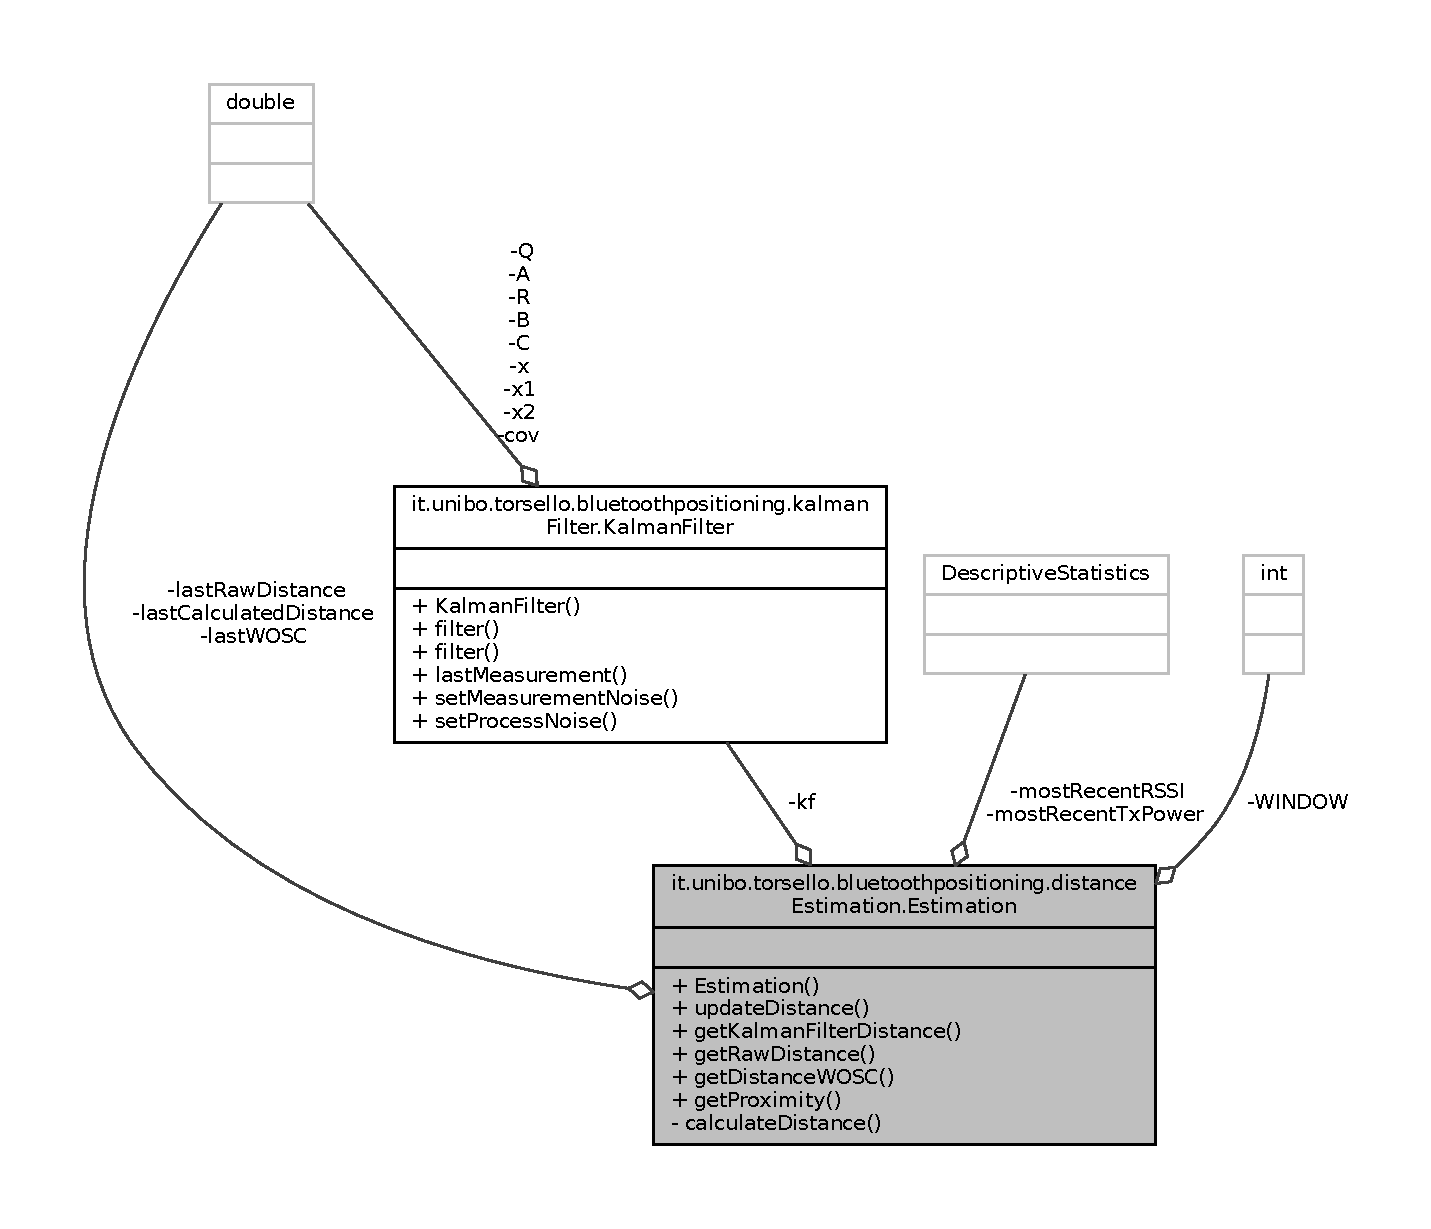
\includegraphics[width=350pt]{classit_1_1unibo_1_1torsello_1_1bluetoothpositioning_1_1distanceEstimation_1_1Estimation__coll__graph}
\end{center}
\end{figure}
\subsubsection*{Membri pubblici}
\begin{DoxyCompactItemize}
\item 
\hyperlink{classit_1_1unibo_1_1torsello_1_1bluetoothpositioning_1_1distanceEstimation_1_1Estimation_abd84ded1e26d40304606ce0572735106_abd84ded1e26d40304606ce0572735106}{Estimation} ()
\item 
void \hyperlink{classit_1_1unibo_1_1torsello_1_1bluetoothpositioning_1_1distanceEstimation_1_1Estimation_aaf86439861db7facf3f5338ec2fc6cde_aaf86439861db7facf3f5338ec2fc6cde}{update\+Distance} (Beacon b, double process\+Noise)
\item 
double \hyperlink{classit_1_1unibo_1_1torsello_1_1bluetoothpositioning_1_1distanceEstimation_1_1Estimation_a985e9b8b61c3d1e917a2e818b5f8b679_a985e9b8b61c3d1e917a2e818b5f8b679}{get\+Kalman\+Filter\+Distance} ()
\item 
double \hyperlink{classit_1_1unibo_1_1torsello_1_1bluetoothpositioning_1_1distanceEstimation_1_1Estimation_ad355b2e850a8d6013ef771eecd740e1b_ad355b2e850a8d6013ef771eecd740e1b}{get\+Raw\+Distance} ()
\item 
double \hyperlink{classit_1_1unibo_1_1torsello_1_1bluetoothpositioning_1_1distanceEstimation_1_1Estimation_a5c7bce21cd77c98a8d1e6df4c930397c_a5c7bce21cd77c98a8d1e6df4c930397c}{get\+Distance\+W\+O\+SC} ()
\item 
String \hyperlink{classit_1_1unibo_1_1torsello_1_1bluetoothpositioning_1_1distanceEstimation_1_1Estimation_a2edfb9f301730647277474c61b41dbd5_a2edfb9f301730647277474c61b41dbd5}{get\+Proximity} ()
\end{DoxyCompactItemize}
\subsubsection*{Membri privati}
\begin{DoxyCompactItemize}
\item 
double \hyperlink{classit_1_1unibo_1_1torsello_1_1bluetoothpositioning_1_1distanceEstimation_1_1Estimation_a6e33d4e0b776517a86c6aa87cd51b66b_a6e33d4e0b776517a86c6aa87cd51b66b}{calculate\+Distance} (double tx\+Power, double rssi)
\end{DoxyCompactItemize}
\subsubsection*{Attributi privati}
\begin{DoxyCompactItemize}
\item 
Descriptive\+Statistics \hyperlink{classit_1_1unibo_1_1torsello_1_1bluetoothpositioning_1_1distanceEstimation_1_1Estimation_a4edd1c580372b087a9d8fc167715088a_a4edd1c580372b087a9d8fc167715088a}{recent\+R\+S\+SI}
\item 
Descriptive\+Statistics \hyperlink{classit_1_1unibo_1_1torsello_1_1bluetoothpositioning_1_1distanceEstimation_1_1Estimation_a4258d96e807fa104223635ecb7ddc940_a4258d96e807fa104223635ecb7ddc940}{recent\+Tx\+Power}
\item 
\hyperlink{classit_1_1unibo_1_1torsello_1_1bluetoothpositioning_1_1kalmanFilter_1_1KFilter}{K\+Filter} \hyperlink{classit_1_1unibo_1_1torsello_1_1bluetoothpositioning_1_1distanceEstimation_1_1Estimation_a93af801219b710f3a048e7db1c7a8982_a93af801219b710f3a048e7db1c7a8982}{kf}
\item 
double \hyperlink{classit_1_1unibo_1_1torsello_1_1bluetoothpositioning_1_1distanceEstimation_1_1Estimation_a7a5514b25ac6495842a53e54319be10d_a7a5514b25ac6495842a53e54319be10d}{distance\+Estimated}
\item 
double \hyperlink{classit_1_1unibo_1_1torsello_1_1bluetoothpositioning_1_1distanceEstimation_1_1Estimation_a5afcd0b9b73a92b64669f060206f35db_a5afcd0b9b73a92b64669f060206f35db}{raw\+Distance\+Estimated}
\item 
double \hyperlink{classit_1_1unibo_1_1torsello_1_1bluetoothpositioning_1_1distanceEstimation_1_1Estimation_a53237b14bc1d27ae4f751b02d798b595_a53237b14bc1d27ae4f751b02d798b595}{W\+O\+SC}
\end{DoxyCompactItemize}


\subsubsection{Descrizione dettagliata}
Created by Federico Torsello. \href{mailto:federico.torsello@studio.unibo.it}{\tt federico.\+torsello@studio.\+unibo.\+it} 

\subsubsection{Documentazione dei costruttori e dei distruttori}
\hypertarget{classit_1_1unibo_1_1torsello_1_1bluetoothpositioning_1_1distanceEstimation_1_1Estimation_abd84ded1e26d40304606ce0572735106_abd84ded1e26d40304606ce0572735106}{}\label{classit_1_1unibo_1_1torsello_1_1bluetoothpositioning_1_1distanceEstimation_1_1Estimation_abd84ded1e26d40304606ce0572735106_abd84ded1e26d40304606ce0572735106} 
\index{it\+::unibo\+::torsello\+::bluetoothpositioning\+::distance\+Estimation\+::\+Estimation@{it\+::unibo\+::torsello\+::bluetoothpositioning\+::distance\+Estimation\+::\+Estimation}!Estimation@{Estimation}}
\index{Estimation@{Estimation}!it\+::unibo\+::torsello\+::bluetoothpositioning\+::distance\+Estimation\+::\+Estimation@{it\+::unibo\+::torsello\+::bluetoothpositioning\+::distance\+Estimation\+::\+Estimation}}
\paragraph{\texorpdfstring{Estimation()}{Estimation()}}
{\footnotesize\ttfamily it.\+unibo.\+torsello.\+bluetoothpositioning.\+distance\+Estimation.\+Estimation.\+Estimation (\begin{DoxyParamCaption}{ }\end{DoxyParamCaption})}


\begin{DoxyCode}
23                         \{
24 
25         \textcolor{comment}{// limit on the number of values that can be stored in the dataset}
26         \hyperlink{classit_1_1unibo_1_1torsello_1_1bluetoothpositioning_1_1distanceEstimation_1_1Estimation_a4edd1c580372b087a9d8fc167715088a_a4edd1c580372b087a9d8fc167715088a}{recentRSSI} = \textcolor{keyword}{new} DescriptiveStatistics();
27         \hyperlink{classit_1_1unibo_1_1torsello_1_1bluetoothpositioning_1_1distanceEstimation_1_1Estimation_a4edd1c580372b087a9d8fc167715088a_a4edd1c580372b087a9d8fc167715088a}{recentRSSI}.setWindowSize(KFilterConstants.WINDOW);
28         \hyperlink{classit_1_1unibo_1_1torsello_1_1bluetoothpositioning_1_1distanceEstimation_1_1Estimation_a4258d96e807fa104223635ecb7ddc940_a4258d96e807fa104223635ecb7ddc940}{recentTxPower} = \textcolor{keyword}{new} DescriptiveStatistics();
29         \hyperlink{classit_1_1unibo_1_1torsello_1_1bluetoothpositioning_1_1distanceEstimation_1_1Estimation_a4258d96e807fa104223635ecb7ddc940_a4258d96e807fa104223635ecb7ddc940}{recentTxPower}.setWindowSize(KFilterConstants.WINDOW);
30 
31         \hyperlink{classit_1_1unibo_1_1torsello_1_1bluetoothpositioning_1_1distanceEstimation_1_1Estimation_a7a5514b25ac6495842a53e54319be10d_a7a5514b25ac6495842a53e54319be10d}{distanceEstimated} = 0;
32         \hyperlink{classit_1_1unibo_1_1torsello_1_1bluetoothpositioning_1_1distanceEstimation_1_1Estimation_a5afcd0b9b73a92b64669f060206f35db_a5afcd0b9b73a92b64669f060206f35db}{rawDistanceEstimated} = 0;
33         \hyperlink{classit_1_1unibo_1_1torsello_1_1bluetoothpositioning_1_1distanceEstimation_1_1Estimation_a53237b14bc1d27ae4f751b02d798b595_a53237b14bc1d27ae4f751b02d798b595}{WOSC} = 0;
34 
35         \hyperlink{classit_1_1unibo_1_1torsello_1_1bluetoothpositioning_1_1distanceEstimation_1_1Estimation_a93af801219b710f3a048e7db1c7a8982_a93af801219b710f3a048e7db1c7a8982}{kf} = \textcolor{keyword}{new} KFilterBuilder()
36                 \textcolor{comment}{// filter for RSSI}
37                 .\hyperlink{classit_1_1unibo_1_1torsello_1_1bluetoothpositioning_1_1kalmanFilter_1_1KFilter_a8dd220ba0a0b0f20c368b13efeb1fe43_a8dd220ba0a0b0f20c368b13efeb1fe43}{R}(KFilterConstants.INITIAL\_PROCESS\_NOISE) \textcolor{comment}{// Initial process noise}
38                 .Q(KFilterConstants.INITIAL\_MEASUREMENT\_NOISE) \textcolor{comment}{// Initial measurement noise}
39                 .build();
40     \}
\end{DoxyCode}


\subsubsection{Documentazione delle funzioni membro}
\hypertarget{classit_1_1unibo_1_1torsello_1_1bluetoothpositioning_1_1distanceEstimation_1_1Estimation_a6e33d4e0b776517a86c6aa87cd51b66b_a6e33d4e0b776517a86c6aa87cd51b66b}{}\label{classit_1_1unibo_1_1torsello_1_1bluetoothpositioning_1_1distanceEstimation_1_1Estimation_a6e33d4e0b776517a86c6aa87cd51b66b_a6e33d4e0b776517a86c6aa87cd51b66b} 
\index{it\+::unibo\+::torsello\+::bluetoothpositioning\+::distance\+Estimation\+::\+Estimation@{it\+::unibo\+::torsello\+::bluetoothpositioning\+::distance\+Estimation\+::\+Estimation}!calculate\+Distance@{calculate\+Distance}}
\index{calculate\+Distance@{calculate\+Distance}!it\+::unibo\+::torsello\+::bluetoothpositioning\+::distance\+Estimation\+::\+Estimation@{it\+::unibo\+::torsello\+::bluetoothpositioning\+::distance\+Estimation\+::\+Estimation}}
\paragraph{\texorpdfstring{calculate\+Distance()}{calculateDistance()}}
{\footnotesize\ttfamily double it.\+unibo.\+torsello.\+bluetoothpositioning.\+distance\+Estimation.\+Estimation.\+calculate\+Distance (\begin{DoxyParamCaption}\item[{double}]{tx\+Power,  }\item[{double}]{rssi }\end{DoxyParamCaption})\hspace{0.3cm}{\ttfamily [private]}}


\begin{DoxyCode}
63                                                                   \{
64 
65         \textcolor{keywordflow}{if} (rssi == 0.0D) \{
66             \textcolor{keywordflow}{return} -1.0D; \textcolor{comment}{// if we cannot determine accuracy, return -1.}
67         \}
68 
69         \textcolor{keywordtype}{double} ratio = (rssi * 1.0D) / txPower;
70         \textcolor{keywordflow}{if} (ratio < 1.0D) \{
71             \textcolor{keywordflow}{return} Math.pow(ratio, 10.0D);
72         \}
73 
74 \textcolor{comment}{//        return (0.89976D * Math.pow(ratio, 7.7095D)) + 0.125D;}
75         \textcolor{keywordflow}{return} (0.89976D * Math.pow(ratio, 7.7095D)) + 0.111D;
76 
77     \textcolor{comment}{/*}
78 \textcolor{comment}{     * RSSI = TxPower - 10 * n * lg(d)}
79 \textcolor{comment}{     * n = 2 (in free space)}
80 \textcolor{comment}{     * d = 10 ^ ((TxPower - RSSI) / (10 * n))}
81 \textcolor{comment}{     */}
82         \textcolor{comment}{// return Math.pow(10D, (txPower - rssi) / (10 * 2));}
83     \}
\end{DoxyCode}
\hypertarget{classit_1_1unibo_1_1torsello_1_1bluetoothpositioning_1_1distanceEstimation_1_1Estimation_a5c7bce21cd77c98a8d1e6df4c930397c_a5c7bce21cd77c98a8d1e6df4c930397c}{}\label{classit_1_1unibo_1_1torsello_1_1bluetoothpositioning_1_1distanceEstimation_1_1Estimation_a5c7bce21cd77c98a8d1e6df4c930397c_a5c7bce21cd77c98a8d1e6df4c930397c} 
\index{it\+::unibo\+::torsello\+::bluetoothpositioning\+::distance\+Estimation\+::\+Estimation@{it\+::unibo\+::torsello\+::bluetoothpositioning\+::distance\+Estimation\+::\+Estimation}!get\+Distance\+W\+O\+SC@{get\+Distance\+W\+O\+SC}}
\index{get\+Distance\+W\+O\+SC@{get\+Distance\+W\+O\+SC}!it\+::unibo\+::torsello\+::bluetoothpositioning\+::distance\+Estimation\+::\+Estimation@{it\+::unibo\+::torsello\+::bluetoothpositioning\+::distance\+Estimation\+::\+Estimation}}
\paragraph{\texorpdfstring{get\+Distance\+W\+O\+S\+C()}{getDistanceWOSC()}}
{\footnotesize\ttfamily double it.\+unibo.\+torsello.\+bluetoothpositioning.\+distance\+Estimation.\+Estimation.\+get\+Distance\+W\+O\+SC (\begin{DoxyParamCaption}{ }\end{DoxyParamCaption})}


\begin{DoxyCode}
93                                     \{
94         \textcolor{keywordflow}{return} \hyperlink{classit_1_1unibo_1_1torsello_1_1bluetoothpositioning_1_1distanceEstimation_1_1Estimation_a53237b14bc1d27ae4f751b02d798b595_a53237b14bc1d27ae4f751b02d798b595}{WOSC};
95     \}
\end{DoxyCode}
\hypertarget{classit_1_1unibo_1_1torsello_1_1bluetoothpositioning_1_1distanceEstimation_1_1Estimation_a985e9b8b61c3d1e917a2e818b5f8b679_a985e9b8b61c3d1e917a2e818b5f8b679}{}\label{classit_1_1unibo_1_1torsello_1_1bluetoothpositioning_1_1distanceEstimation_1_1Estimation_a985e9b8b61c3d1e917a2e818b5f8b679_a985e9b8b61c3d1e917a2e818b5f8b679} 
\index{it\+::unibo\+::torsello\+::bluetoothpositioning\+::distance\+Estimation\+::\+Estimation@{it\+::unibo\+::torsello\+::bluetoothpositioning\+::distance\+Estimation\+::\+Estimation}!get\+Kalman\+Filter\+Distance@{get\+Kalman\+Filter\+Distance}}
\index{get\+Kalman\+Filter\+Distance@{get\+Kalman\+Filter\+Distance}!it\+::unibo\+::torsello\+::bluetoothpositioning\+::distance\+Estimation\+::\+Estimation@{it\+::unibo\+::torsello\+::bluetoothpositioning\+::distance\+Estimation\+::\+Estimation}}
\paragraph{\texorpdfstring{get\+Kalman\+Filter\+Distance()}{getKalmanFilterDistance()}}
{\footnotesize\ttfamily double it.\+unibo.\+torsello.\+bluetoothpositioning.\+distance\+Estimation.\+Estimation.\+get\+Kalman\+Filter\+Distance (\begin{DoxyParamCaption}{ }\end{DoxyParamCaption})}


\begin{DoxyCode}
85                                             \{
86         \textcolor{keywordflow}{return} \hyperlink{classit_1_1unibo_1_1torsello_1_1bluetoothpositioning_1_1distanceEstimation_1_1Estimation_a7a5514b25ac6495842a53e54319be10d_a7a5514b25ac6495842a53e54319be10d}{distanceEstimated};
87     \}
\end{DoxyCode}
\hypertarget{classit_1_1unibo_1_1torsello_1_1bluetoothpositioning_1_1distanceEstimation_1_1Estimation_a2edfb9f301730647277474c61b41dbd5_a2edfb9f301730647277474c61b41dbd5}{}\label{classit_1_1unibo_1_1torsello_1_1bluetoothpositioning_1_1distanceEstimation_1_1Estimation_a2edfb9f301730647277474c61b41dbd5_a2edfb9f301730647277474c61b41dbd5} 
\index{it\+::unibo\+::torsello\+::bluetoothpositioning\+::distance\+Estimation\+::\+Estimation@{it\+::unibo\+::torsello\+::bluetoothpositioning\+::distance\+Estimation\+::\+Estimation}!get\+Proximity@{get\+Proximity}}
\index{get\+Proximity@{get\+Proximity}!it\+::unibo\+::torsello\+::bluetoothpositioning\+::distance\+Estimation\+::\+Estimation@{it\+::unibo\+::torsello\+::bluetoothpositioning\+::distance\+Estimation\+::\+Estimation}}
\paragraph{\texorpdfstring{get\+Proximity()}{getProximity()}}
{\footnotesize\ttfamily String it.\+unibo.\+torsello.\+bluetoothpositioning.\+distance\+Estimation.\+Estimation.\+get\+Proximity (\begin{DoxyParamCaption}{ }\end{DoxyParamCaption})}


\begin{DoxyCode}
97                                  \{
98         \textcolor{keywordtype}{double} proximity = \hyperlink{classit_1_1unibo_1_1torsello_1_1bluetoothpositioning_1_1distanceEstimation_1_1Estimation_a7a5514b25ac6495842a53e54319be10d_a7a5514b25ac6495842a53e54319be10d}{distanceEstimated};
99         String accuracy;
100 
101         \textcolor{keywordflow}{if} (proximity <= 0) \{
102             accuracy = \textcolor{stringliteral}{"unknown"};
103         \} \textcolor{keywordflow}{else} \textcolor{keywordflow}{if} (proximity <= 0.5) \{
104             accuracy = \textcolor{stringliteral}{"immediate"};
105         \} \textcolor{keywordflow}{else} \textcolor{keywordflow}{if} (proximity <= 4.0) \{
106             accuracy = \textcolor{stringliteral}{"near"};
107         \} \textcolor{keywordflow}{else} \{
108             accuracy = \textcolor{stringliteral}{"far"};
109         \}
110         \textcolor{keywordflow}{return} accuracy;
111     \}
\end{DoxyCode}
\hypertarget{classit_1_1unibo_1_1torsello_1_1bluetoothpositioning_1_1distanceEstimation_1_1Estimation_ad355b2e850a8d6013ef771eecd740e1b_ad355b2e850a8d6013ef771eecd740e1b}{}\label{classit_1_1unibo_1_1torsello_1_1bluetoothpositioning_1_1distanceEstimation_1_1Estimation_ad355b2e850a8d6013ef771eecd740e1b_ad355b2e850a8d6013ef771eecd740e1b} 
\index{it\+::unibo\+::torsello\+::bluetoothpositioning\+::distance\+Estimation\+::\+Estimation@{it\+::unibo\+::torsello\+::bluetoothpositioning\+::distance\+Estimation\+::\+Estimation}!get\+Raw\+Distance@{get\+Raw\+Distance}}
\index{get\+Raw\+Distance@{get\+Raw\+Distance}!it\+::unibo\+::torsello\+::bluetoothpositioning\+::distance\+Estimation\+::\+Estimation@{it\+::unibo\+::torsello\+::bluetoothpositioning\+::distance\+Estimation\+::\+Estimation}}
\paragraph{\texorpdfstring{get\+Raw\+Distance()}{getRawDistance()}}
{\footnotesize\ttfamily double it.\+unibo.\+torsello.\+bluetoothpositioning.\+distance\+Estimation.\+Estimation.\+get\+Raw\+Distance (\begin{DoxyParamCaption}{ }\end{DoxyParamCaption})}


\begin{DoxyCode}
89                                    \{
90         \textcolor{keywordflow}{return} \hyperlink{classit_1_1unibo_1_1torsello_1_1bluetoothpositioning_1_1distanceEstimation_1_1Estimation_a5afcd0b9b73a92b64669f060206f35db_a5afcd0b9b73a92b64669f060206f35db}{rawDistanceEstimated};
91     \}
\end{DoxyCode}
\hypertarget{classit_1_1unibo_1_1torsello_1_1bluetoothpositioning_1_1distanceEstimation_1_1Estimation_aaf86439861db7facf3f5338ec2fc6cde_aaf86439861db7facf3f5338ec2fc6cde}{}\label{classit_1_1unibo_1_1torsello_1_1bluetoothpositioning_1_1distanceEstimation_1_1Estimation_aaf86439861db7facf3f5338ec2fc6cde_aaf86439861db7facf3f5338ec2fc6cde} 
\index{it\+::unibo\+::torsello\+::bluetoothpositioning\+::distance\+Estimation\+::\+Estimation@{it\+::unibo\+::torsello\+::bluetoothpositioning\+::distance\+Estimation\+::\+Estimation}!update\+Distance@{update\+Distance}}
\index{update\+Distance@{update\+Distance}!it\+::unibo\+::torsello\+::bluetoothpositioning\+::distance\+Estimation\+::\+Estimation@{it\+::unibo\+::torsello\+::bluetoothpositioning\+::distance\+Estimation\+::\+Estimation}}
\paragraph{\texorpdfstring{update\+Distance()}{updateDistance()}}
{\footnotesize\ttfamily void it.\+unibo.\+torsello.\+bluetoothpositioning.\+distance\+Estimation.\+Estimation.\+update\+Distance (\begin{DoxyParamCaption}\item[{Beacon}]{b,  }\item[{double}]{process\+Noise }\end{DoxyParamCaption})}


\begin{DoxyCode}
42                                                               \{
43 
44         \hyperlink{classit_1_1unibo_1_1torsello_1_1bluetoothpositioning_1_1distanceEstimation_1_1Estimation_a4edd1c580372b087a9d8fc167715088a_a4edd1c580372b087a9d8fc167715088a}{recentRSSI}.addValue(b.getRssi());
45         \hyperlink{classit_1_1unibo_1_1torsello_1_1bluetoothpositioning_1_1distanceEstimation_1_1Estimation_a4258d96e807fa104223635ecb7ddc940_a4258d96e807fa104223635ecb7ddc940}{recentTxPower}.addValue(b.getTxPower());
46 
47         \textcolor{comment}{// Update measurement noise continually}
48         \textcolor{keywordtype}{double} mNoise = Math.sqrt((100 * 9 / Math.log(10)) *
49                 Math.log(1 + Math.pow(\hyperlink{classit_1_1unibo_1_1torsello_1_1bluetoothpositioning_1_1distanceEstimation_1_1Estimation_a4edd1c580372b087a9d8fc167715088a_a4edd1c580372b087a9d8fc167715088a}{recentRSSI}.getMean() / 
      \hyperlink{classit_1_1unibo_1_1torsello_1_1bluetoothpositioning_1_1distanceEstimation_1_1Estimation_a4edd1c580372b087a9d8fc167715088a_a4edd1c580372b087a9d8fc167715088a}{recentRSSI}.getStandardDeviation(), 2)));
50 
51         \textcolor{keywordflow}{if} (!Double.isInfinite(mNoise) && !Double.isNaN(mNoise)) \{
52             \hyperlink{classit_1_1unibo_1_1torsello_1_1bluetoothpositioning_1_1distanceEstimation_1_1Estimation_a93af801219b710f3a048e7db1c7a8982_a93af801219b710f3a048e7db1c7a8982}{kf}.\hyperlink{classit_1_1unibo_1_1torsello_1_1bluetoothpositioning_1_1kalmanFilter_1_1KFilter_a0ed62a630ff52aacdcd8832b9416f406_a0ed62a630ff52aacdcd8832b9416f406}{setMeasurementNoise}(mNoise);
53         \}
54 
55         \hyperlink{classit_1_1unibo_1_1torsello_1_1bluetoothpositioning_1_1distanceEstimation_1_1Estimation_a93af801219b710f3a048e7db1c7a8982_a93af801219b710f3a048e7db1c7a8982}{kf}.\hyperlink{classit_1_1unibo_1_1torsello_1_1bluetoothpositioning_1_1kalmanFilter_1_1KFilter_a7651339cfddb4cdaa1e47906b27745fc_a7651339cfddb4cdaa1e47906b27745fc}{setProcessNoise}(processNoise);
56         \textcolor{keywordtype}{double} lastFilteredReading = \hyperlink{classit_1_1unibo_1_1torsello_1_1bluetoothpositioning_1_1distanceEstimation_1_1Estimation_a93af801219b710f3a048e7db1c7a8982_a93af801219b710f3a048e7db1c7a8982}{kf}.\hyperlink{classit_1_1unibo_1_1torsello_1_1bluetoothpositioning_1_1kalmanFilter_1_1KFilter_a6904818e94d959f8e25a8699d6885c21_a6904818e94d959f8e25a8699d6885c21}{filter}(\hyperlink{classit_1_1unibo_1_1torsello_1_1bluetoothpositioning_1_1distanceEstimation_1_1Estimation_a4edd1c580372b087a9d8fc167715088a_a4edd1c580372b087a9d8fc167715088a}{recentRSSI}.getPercentile(50));
57         \hyperlink{classit_1_1unibo_1_1torsello_1_1bluetoothpositioning_1_1distanceEstimation_1_1Estimation_a7a5514b25ac6495842a53e54319be10d_a7a5514b25ac6495842a53e54319be10d}{distanceEstimated} = \hyperlink{classit_1_1unibo_1_1torsello_1_1bluetoothpositioning_1_1distanceEstimation_1_1Estimation_a6e33d4e0b776517a86c6aa87cd51b66b_a6e33d4e0b776517a86c6aa87cd51b66b}{calculateDistance}(
      \hyperlink{classit_1_1unibo_1_1torsello_1_1bluetoothpositioning_1_1distanceEstimation_1_1Estimation_a4258d96e807fa104223635ecb7ddc940_a4258d96e807fa104223635ecb7ddc940}{recentTxPower}.getPercentile(50), lastFilteredReading);
58         \hyperlink{classit_1_1unibo_1_1torsello_1_1bluetoothpositioning_1_1distanceEstimation_1_1Estimation_a5afcd0b9b73a92b64669f060206f35db_a5afcd0b9b73a92b64669f060206f35db}{rawDistanceEstimated} = \hyperlink{classit_1_1unibo_1_1torsello_1_1bluetoothpositioning_1_1distanceEstimation_1_1Estimation_a6e33d4e0b776517a86c6aa87cd51b66b_a6e33d4e0b776517a86c6aa87cd51b66b}{calculateDistance}(b.getTxPower(), b.
      getRssi());
59         \hyperlink{classit_1_1unibo_1_1torsello_1_1bluetoothpositioning_1_1distanceEstimation_1_1Estimation_a53237b14bc1d27ae4f751b02d798b595_a53237b14bc1d27ae4f751b02d798b595}{WOSC} = \hyperlink{classit_1_1unibo_1_1torsello_1_1bluetoothpositioning_1_1distanceEstimation_1_1Estimation_a6e33d4e0b776517a86c6aa87cd51b66b_a6e33d4e0b776517a86c6aa87cd51b66b}{calculateDistance}(b.getTxPower(), lastFilteredReading);
60     \}
\end{DoxyCode}


\subsubsection{Documentazione dei membri dato}
\hypertarget{classit_1_1unibo_1_1torsello_1_1bluetoothpositioning_1_1distanceEstimation_1_1Estimation_a7a5514b25ac6495842a53e54319be10d_a7a5514b25ac6495842a53e54319be10d}{}\label{classit_1_1unibo_1_1torsello_1_1bluetoothpositioning_1_1distanceEstimation_1_1Estimation_a7a5514b25ac6495842a53e54319be10d_a7a5514b25ac6495842a53e54319be10d} 
\index{it\+::unibo\+::torsello\+::bluetoothpositioning\+::distance\+Estimation\+::\+Estimation@{it\+::unibo\+::torsello\+::bluetoothpositioning\+::distance\+Estimation\+::\+Estimation}!distance\+Estimated@{distance\+Estimated}}
\index{distance\+Estimated@{distance\+Estimated}!it\+::unibo\+::torsello\+::bluetoothpositioning\+::distance\+Estimation\+::\+Estimation@{it\+::unibo\+::torsello\+::bluetoothpositioning\+::distance\+Estimation\+::\+Estimation}}
\paragraph{\texorpdfstring{distance\+Estimated}{distanceEstimated}}
{\footnotesize\ttfamily double it.\+unibo.\+torsello.\+bluetoothpositioning.\+distance\+Estimation.\+Estimation.\+distance\+Estimated\hspace{0.3cm}{\ttfamily [private]}}

\hypertarget{classit_1_1unibo_1_1torsello_1_1bluetoothpositioning_1_1distanceEstimation_1_1Estimation_a93af801219b710f3a048e7db1c7a8982_a93af801219b710f3a048e7db1c7a8982}{}\label{classit_1_1unibo_1_1torsello_1_1bluetoothpositioning_1_1distanceEstimation_1_1Estimation_a93af801219b710f3a048e7db1c7a8982_a93af801219b710f3a048e7db1c7a8982} 
\index{it\+::unibo\+::torsello\+::bluetoothpositioning\+::distance\+Estimation\+::\+Estimation@{it\+::unibo\+::torsello\+::bluetoothpositioning\+::distance\+Estimation\+::\+Estimation}!kf@{kf}}
\index{kf@{kf}!it\+::unibo\+::torsello\+::bluetoothpositioning\+::distance\+Estimation\+::\+Estimation@{it\+::unibo\+::torsello\+::bluetoothpositioning\+::distance\+Estimation\+::\+Estimation}}
\paragraph{\texorpdfstring{kf}{kf}}
{\footnotesize\ttfamily \hyperlink{classit_1_1unibo_1_1torsello_1_1bluetoothpositioning_1_1kalmanFilter_1_1KFilter}{K\+Filter} it.\+unibo.\+torsello.\+bluetoothpositioning.\+distance\+Estimation.\+Estimation.\+kf\hspace{0.3cm}{\ttfamily [private]}}

\hypertarget{classit_1_1unibo_1_1torsello_1_1bluetoothpositioning_1_1distanceEstimation_1_1Estimation_a5afcd0b9b73a92b64669f060206f35db_a5afcd0b9b73a92b64669f060206f35db}{}\label{classit_1_1unibo_1_1torsello_1_1bluetoothpositioning_1_1distanceEstimation_1_1Estimation_a5afcd0b9b73a92b64669f060206f35db_a5afcd0b9b73a92b64669f060206f35db} 
\index{it\+::unibo\+::torsello\+::bluetoothpositioning\+::distance\+Estimation\+::\+Estimation@{it\+::unibo\+::torsello\+::bluetoothpositioning\+::distance\+Estimation\+::\+Estimation}!raw\+Distance\+Estimated@{raw\+Distance\+Estimated}}
\index{raw\+Distance\+Estimated@{raw\+Distance\+Estimated}!it\+::unibo\+::torsello\+::bluetoothpositioning\+::distance\+Estimation\+::\+Estimation@{it\+::unibo\+::torsello\+::bluetoothpositioning\+::distance\+Estimation\+::\+Estimation}}
\paragraph{\texorpdfstring{raw\+Distance\+Estimated}{rawDistanceEstimated}}
{\footnotesize\ttfamily double it.\+unibo.\+torsello.\+bluetoothpositioning.\+distance\+Estimation.\+Estimation.\+raw\+Distance\+Estimated\hspace{0.3cm}{\ttfamily [private]}}

\hypertarget{classit_1_1unibo_1_1torsello_1_1bluetoothpositioning_1_1distanceEstimation_1_1Estimation_a4edd1c580372b087a9d8fc167715088a_a4edd1c580372b087a9d8fc167715088a}{}\label{classit_1_1unibo_1_1torsello_1_1bluetoothpositioning_1_1distanceEstimation_1_1Estimation_a4edd1c580372b087a9d8fc167715088a_a4edd1c580372b087a9d8fc167715088a} 
\index{it\+::unibo\+::torsello\+::bluetoothpositioning\+::distance\+Estimation\+::\+Estimation@{it\+::unibo\+::torsello\+::bluetoothpositioning\+::distance\+Estimation\+::\+Estimation}!recent\+R\+S\+SI@{recent\+R\+S\+SI}}
\index{recent\+R\+S\+SI@{recent\+R\+S\+SI}!it\+::unibo\+::torsello\+::bluetoothpositioning\+::distance\+Estimation\+::\+Estimation@{it\+::unibo\+::torsello\+::bluetoothpositioning\+::distance\+Estimation\+::\+Estimation}}
\paragraph{\texorpdfstring{recent\+R\+S\+SI}{recentRSSI}}
{\footnotesize\ttfamily Descriptive\+Statistics it.\+unibo.\+torsello.\+bluetoothpositioning.\+distance\+Estimation.\+Estimation.\+recent\+R\+S\+SI\hspace{0.3cm}{\ttfamily [private]}}

\hypertarget{classit_1_1unibo_1_1torsello_1_1bluetoothpositioning_1_1distanceEstimation_1_1Estimation_a4258d96e807fa104223635ecb7ddc940_a4258d96e807fa104223635ecb7ddc940}{}\label{classit_1_1unibo_1_1torsello_1_1bluetoothpositioning_1_1distanceEstimation_1_1Estimation_a4258d96e807fa104223635ecb7ddc940_a4258d96e807fa104223635ecb7ddc940} 
\index{it\+::unibo\+::torsello\+::bluetoothpositioning\+::distance\+Estimation\+::\+Estimation@{it\+::unibo\+::torsello\+::bluetoothpositioning\+::distance\+Estimation\+::\+Estimation}!recent\+Tx\+Power@{recent\+Tx\+Power}}
\index{recent\+Tx\+Power@{recent\+Tx\+Power}!it\+::unibo\+::torsello\+::bluetoothpositioning\+::distance\+Estimation\+::\+Estimation@{it\+::unibo\+::torsello\+::bluetoothpositioning\+::distance\+Estimation\+::\+Estimation}}
\paragraph{\texorpdfstring{recent\+Tx\+Power}{recentTxPower}}
{\footnotesize\ttfamily Descriptive\+Statistics it.\+unibo.\+torsello.\+bluetoothpositioning.\+distance\+Estimation.\+Estimation.\+recent\+Tx\+Power\hspace{0.3cm}{\ttfamily [private]}}

\hypertarget{classit_1_1unibo_1_1torsello_1_1bluetoothpositioning_1_1distanceEstimation_1_1Estimation_a53237b14bc1d27ae4f751b02d798b595_a53237b14bc1d27ae4f751b02d798b595}{}\label{classit_1_1unibo_1_1torsello_1_1bluetoothpositioning_1_1distanceEstimation_1_1Estimation_a53237b14bc1d27ae4f751b02d798b595_a53237b14bc1d27ae4f751b02d798b595} 
\index{it\+::unibo\+::torsello\+::bluetoothpositioning\+::distance\+Estimation\+::\+Estimation@{it\+::unibo\+::torsello\+::bluetoothpositioning\+::distance\+Estimation\+::\+Estimation}!W\+O\+SC@{W\+O\+SC}}
\index{W\+O\+SC@{W\+O\+SC}!it\+::unibo\+::torsello\+::bluetoothpositioning\+::distance\+Estimation\+::\+Estimation@{it\+::unibo\+::torsello\+::bluetoothpositioning\+::distance\+Estimation\+::\+Estimation}}
\paragraph{\texorpdfstring{W\+O\+SC}{WOSC}}
{\footnotesize\ttfamily double it.\+unibo.\+torsello.\+bluetoothpositioning.\+distance\+Estimation.\+Estimation.\+W\+O\+SC\hspace{0.3cm}{\ttfamily [private]}}



La documentazione per questa classe è stata generata a partire dal seguente file\+:\begin{DoxyCompactItemize}
\item 
\hyperlink{Estimation_8java}{Estimation.\+java}\end{DoxyCompactItemize}

\hypertarget{classit_1_1unibo_1_1torsello_1_1bluetoothpositioning_1_1extra_1_1FABBehavior}{}\subsection{Riferimenti per la classe it.\+unibo.\+torsello.\+bluetoothpositioning.\+extra.\+F\+A\+B\+Behavior}
\label{classit_1_1unibo_1_1torsello_1_1bluetoothpositioning_1_1extra_1_1FABBehavior}\index{it.\+unibo.\+torsello.\+bluetoothpositioning.\+extra.\+F\+A\+B\+Behavior@{it.\+unibo.\+torsello.\+bluetoothpositioning.\+extra.\+F\+A\+B\+Behavior}}


Diagramma delle classi per it.\+unibo.\+torsello.\+bluetoothpositioning.\+extra.\+F\+A\+B\+Behavior
\nopagebreak
\begin{figure}[H]
\begin{center}
\leavevmode
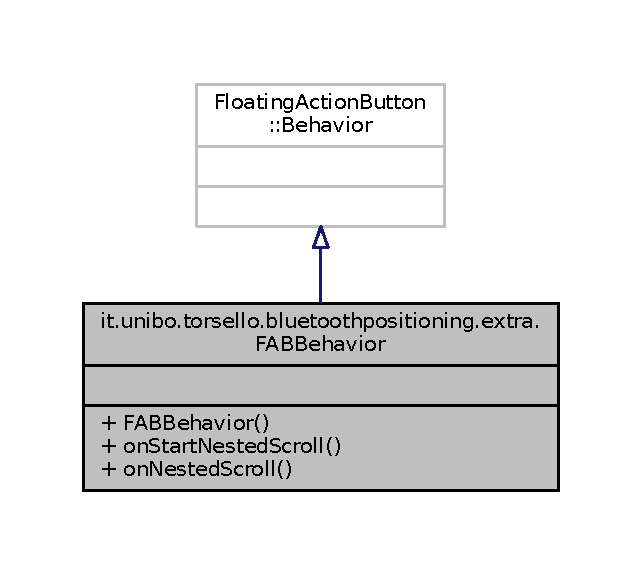
\includegraphics[width=308pt]{classit_1_1unibo_1_1torsello_1_1bluetoothpositioning_1_1extra_1_1FABBehavior__inherit__graph}
\end{center}
\end{figure}


Diagramma di collaborazione per it.\+unibo.\+torsello.\+bluetoothpositioning.\+extra.\+F\+A\+B\+Behavior\+:
\nopagebreak
\begin{figure}[H]
\begin{center}
\leavevmode
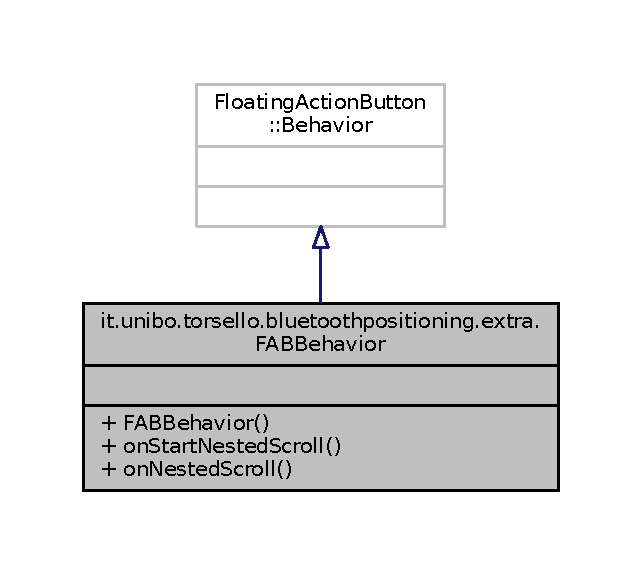
\includegraphics[width=308pt]{classit_1_1unibo_1_1torsello_1_1bluetoothpositioning_1_1extra_1_1FABBehavior__coll__graph}
\end{center}
\end{figure}
\subsubsection*{Membri pubblici}
\begin{DoxyCompactItemize}
\item 
\hyperlink{classit_1_1unibo_1_1torsello_1_1bluetoothpositioning_1_1extra_1_1FABBehavior_ae703e3a3d6d647561f7b41a0eb94a9f0_ae703e3a3d6d647561f7b41a0eb94a9f0}{F\+A\+B\+Behavior} (Context context, Attribute\+Set attrs)
\item 
boolean \hyperlink{classit_1_1unibo_1_1torsello_1_1bluetoothpositioning_1_1extra_1_1FABBehavior_a5c6501a08ec79dd6bd92106b72c14979_a5c6501a08ec79dd6bd92106b72c14979}{on\+Start\+Nested\+Scroll} (Coordinator\+Layout coordinator\+Layout, final Floating\+Action\+Button child, View direct\+Target\+Child, View target, int nested\+Scroll\+Axes)
\item 
void \hyperlink{classit_1_1unibo_1_1torsello_1_1bluetoothpositioning_1_1extra_1_1FABBehavior_ab4208eb2a50a8e79e0a80089f398a5b9_ab4208eb2a50a8e79e0a80089f398a5b9}{on\+Nested\+Scroll} (Coordinator\+Layout coordinator\+Layout, final Floating\+Action\+Button child, View target, int dx\+Consumed, int dy\+Consumed, int dx\+Unconsumed, int dy\+Unconsumed)
\end{DoxyCompactItemize}


\subsubsection{Descrizione dettagliata}
Created by Federico Torsello. \href{mailto:federico.torsello@studio.unibo.it}{\tt federico.\+torsello@studio.\+unibo.\+it} 

\subsubsection{Documentazione dei costruttori e dei distruttori}
\hypertarget{classit_1_1unibo_1_1torsello_1_1bluetoothpositioning_1_1extra_1_1FABBehavior_ae703e3a3d6d647561f7b41a0eb94a9f0_ae703e3a3d6d647561f7b41a0eb94a9f0}{}\label{classit_1_1unibo_1_1torsello_1_1bluetoothpositioning_1_1extra_1_1FABBehavior_ae703e3a3d6d647561f7b41a0eb94a9f0_ae703e3a3d6d647561f7b41a0eb94a9f0} 
\index{it\+::unibo\+::torsello\+::bluetoothpositioning\+::extra\+::\+F\+A\+B\+Behavior@{it\+::unibo\+::torsello\+::bluetoothpositioning\+::extra\+::\+F\+A\+B\+Behavior}!F\+A\+B\+Behavior@{F\+A\+B\+Behavior}}
\index{F\+A\+B\+Behavior@{F\+A\+B\+Behavior}!it\+::unibo\+::torsello\+::bluetoothpositioning\+::extra\+::\+F\+A\+B\+Behavior@{it\+::unibo\+::torsello\+::bluetoothpositioning\+::extra\+::\+F\+A\+B\+Behavior}}
\paragraph{\texorpdfstring{F\+A\+B\+Behavior()}{FABBehavior()}}
{\footnotesize\ttfamily it.\+unibo.\+torsello.\+bluetoothpositioning.\+extra.\+F\+A\+B\+Behavior.\+F\+A\+B\+Behavior (\begin{DoxyParamCaption}\item[{Context}]{context,  }\item[{Attribute\+Set}]{attrs }\end{DoxyParamCaption})}


\begin{DoxyCode}
18                                                             \{
19         super();
20     \}
\end{DoxyCode}


\subsubsection{Documentazione delle funzioni membro}
\hypertarget{classit_1_1unibo_1_1torsello_1_1bluetoothpositioning_1_1extra_1_1FABBehavior_ab4208eb2a50a8e79e0a80089f398a5b9_ab4208eb2a50a8e79e0a80089f398a5b9}{}\label{classit_1_1unibo_1_1torsello_1_1bluetoothpositioning_1_1extra_1_1FABBehavior_ab4208eb2a50a8e79e0a80089f398a5b9_ab4208eb2a50a8e79e0a80089f398a5b9} 
\index{it\+::unibo\+::torsello\+::bluetoothpositioning\+::extra\+::\+F\+A\+B\+Behavior@{it\+::unibo\+::torsello\+::bluetoothpositioning\+::extra\+::\+F\+A\+B\+Behavior}!on\+Nested\+Scroll@{on\+Nested\+Scroll}}
\index{on\+Nested\+Scroll@{on\+Nested\+Scroll}!it\+::unibo\+::torsello\+::bluetoothpositioning\+::extra\+::\+F\+A\+B\+Behavior@{it\+::unibo\+::torsello\+::bluetoothpositioning\+::extra\+::\+F\+A\+B\+Behavior}}
\paragraph{\texorpdfstring{on\+Nested\+Scroll()}{onNestedScroll()}}
{\footnotesize\ttfamily void it.\+unibo.\+torsello.\+bluetoothpositioning.\+extra.\+F\+A\+B\+Behavior.\+on\+Nested\+Scroll (\begin{DoxyParamCaption}\item[{Coordinator\+Layout}]{coordinator\+Layout,  }\item[{final Floating\+Action\+Button}]{child,  }\item[{View}]{target,  }\item[{int}]{dx\+Consumed,  }\item[{int}]{dy\+Consumed,  }\item[{int}]{dx\+Unconsumed,  }\item[{int}]{dy\+Unconsumed }\end{DoxyParamCaption})}


\begin{DoxyCode}
34                                                                                                            
           \{
35         super.onNestedScroll(coordinatorLayout, child, target, dxConsumed, dyConsumed, dxUnconsumed,
36                 dyUnconsumed);
37 
38         \textcolor{keywordflow}{if} ((dyConsumed > 0 || dyUnconsumed == 0) && child.getVisibility() == View.VISIBLE) \{
39             child.hide();
40             \textcolor{keyword}{new} Handler().postDelayed(\textcolor{keyword}{new} Runnable() \{
41                 @Override
42                 \textcolor{keyword}{public} \textcolor{keywordtype}{void} run() \{
43                     child.show();
44                 \}
45             \}, 1000);
46         \}
47     \}
\end{DoxyCode}
\hypertarget{classit_1_1unibo_1_1torsello_1_1bluetoothpositioning_1_1extra_1_1FABBehavior_a5c6501a08ec79dd6bd92106b72c14979_a5c6501a08ec79dd6bd92106b72c14979}{}\label{classit_1_1unibo_1_1torsello_1_1bluetoothpositioning_1_1extra_1_1FABBehavior_a5c6501a08ec79dd6bd92106b72c14979_a5c6501a08ec79dd6bd92106b72c14979} 
\index{it\+::unibo\+::torsello\+::bluetoothpositioning\+::extra\+::\+F\+A\+B\+Behavior@{it\+::unibo\+::torsello\+::bluetoothpositioning\+::extra\+::\+F\+A\+B\+Behavior}!on\+Start\+Nested\+Scroll@{on\+Start\+Nested\+Scroll}}
\index{on\+Start\+Nested\+Scroll@{on\+Start\+Nested\+Scroll}!it\+::unibo\+::torsello\+::bluetoothpositioning\+::extra\+::\+F\+A\+B\+Behavior@{it\+::unibo\+::torsello\+::bluetoothpositioning\+::extra\+::\+F\+A\+B\+Behavior}}
\paragraph{\texorpdfstring{on\+Start\+Nested\+Scroll()}{onStartNestedScroll()}}
{\footnotesize\ttfamily boolean it.\+unibo.\+torsello.\+bluetoothpositioning.\+extra.\+F\+A\+B\+Behavior.\+on\+Start\+Nested\+Scroll (\begin{DoxyParamCaption}\item[{Coordinator\+Layout}]{coordinator\+Layout,  }\item[{final Floating\+Action\+Button}]{child,  }\item[{View}]{direct\+Target\+Child,  }\item[{View}]{target,  }\item[{int}]{nested\+Scroll\+Axes }\end{DoxyParamCaption})}


\begin{DoxyCode}
24                                                                                                   \{
25 
26 \textcolor{comment}{//        return nestedScrollAxes == ViewCompat.SCROLL\_AXIS\_VERTICAL ||}
27 \textcolor{comment}{//                super.onStartNestedScroll(coordinatorLayout, child, directTargetChild, target,}
28 \textcolor{comment}{//                        nestedScrollAxes);}
29         \textcolor{keywordflow}{return} \textcolor{keyword}{true};
30     \}
\end{DoxyCode}


La documentazione per questa classe è stata generata a partire dal seguente file\+:\begin{DoxyCompactItemize}
\item 
\hyperlink{FABBehavior_8java}{F\+A\+B\+Behavior.\+java}\end{DoxyCompactItemize}

\hypertarget{classit_1_1unibo_1_1torsello_1_1bluetoothpositioning_1_1filters_1_1kalmanFilter_1_1KFilter}{}\subsection{Riferimenti per la classe it.\+unibo.\+torsello.\+bluetoothpositioning.\+filters.\+kalman\+Filter.\+K\+Filter}
\label{classit_1_1unibo_1_1torsello_1_1bluetoothpositioning_1_1filters_1_1kalmanFilter_1_1KFilter}\index{it.\+unibo.\+torsello.\+bluetoothpositioning.\+filters.\+kalman\+Filter.\+K\+Filter@{it.\+unibo.\+torsello.\+bluetoothpositioning.\+filters.\+kalman\+Filter.\+K\+Filter}}


Diagramma di collaborazione per it.\+unibo.\+torsello.\+bluetoothpositioning.\+filters.\+kalman\+Filter.\+K\+Filter\+:
\nopagebreak
\begin{figure}[H]
\begin{center}
\leavevmode
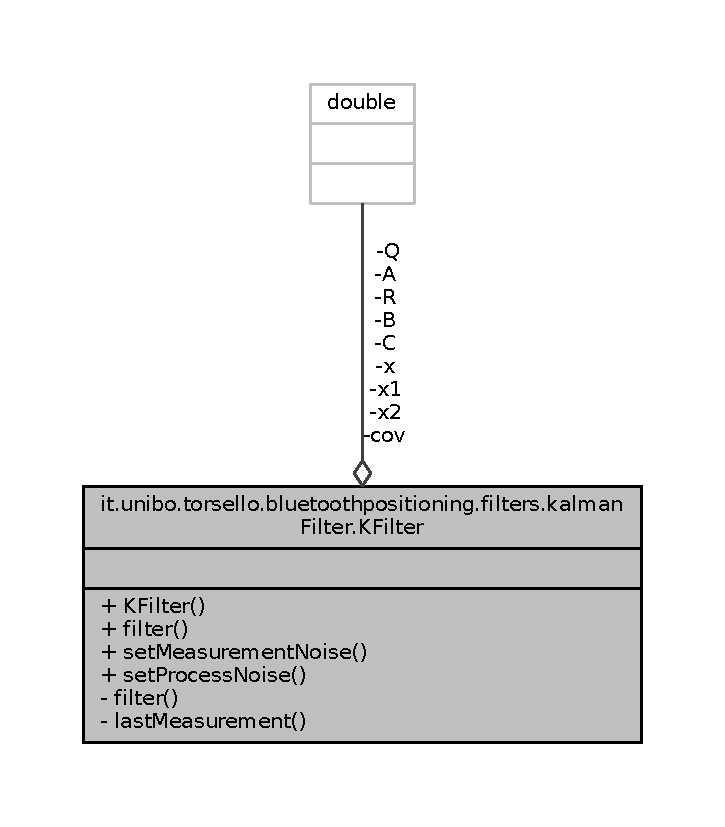
\includegraphics[width=348pt]{classit_1_1unibo_1_1torsello_1_1bluetoothpositioning_1_1filters_1_1kalmanFilter_1_1KFilter__coll__graph}
\end{center}
\end{figure}
\subsubsection*{Membri pubblici}
\begin{DoxyCompactItemize}
\item 
\hyperlink{classit_1_1unibo_1_1torsello_1_1bluetoothpositioning_1_1filters_1_1kalmanFilter_1_1KFilter_a645ffd2ce2f433212caf4e99a2839c26_a645ffd2ce2f433212caf4e99a2839c26}{K\+Filter} (double \hyperlink{classit_1_1unibo_1_1torsello_1_1bluetoothpositioning_1_1filters_1_1kalmanFilter_1_1KFilter_ac5b2a95b9934717adadb214003d7e7bc_ac5b2a95b9934717adadb214003d7e7bc}{R}, double \hyperlink{classit_1_1unibo_1_1torsello_1_1bluetoothpositioning_1_1filters_1_1kalmanFilter_1_1KFilter_a214fff6f5bc8eed06a7be5000d4ccfef_a214fff6f5bc8eed06a7be5000d4ccfef}{Q}, double \hyperlink{classit_1_1unibo_1_1torsello_1_1bluetoothpositioning_1_1filters_1_1kalmanFilter_1_1KFilter_a761ff20b52df6e05a2cf023d793e3cc2_a761ff20b52df6e05a2cf023d793e3cc2}{A}, double \hyperlink{classit_1_1unibo_1_1torsello_1_1bluetoothpositioning_1_1filters_1_1kalmanFilter_1_1KFilter_adde4f664a3dd2e0c1f2c378b3d28c3da_adde4f664a3dd2e0c1f2c378b3d28c3da}{B}, double \hyperlink{classit_1_1unibo_1_1torsello_1_1bluetoothpositioning_1_1filters_1_1kalmanFilter_1_1KFilter_a67a040dd80123bdb5393070b299fc2bf_a67a040dd80123bdb5393070b299fc2bf}{C})
\item 
double \hyperlink{classit_1_1unibo_1_1torsello_1_1bluetoothpositioning_1_1filters_1_1kalmanFilter_1_1KFilter_a58554e5bc1f7e2c5692bfaf2ea496a45_a58554e5bc1f7e2c5692bfaf2ea496a45}{filter} (double z)
\item 
void \hyperlink{classit_1_1unibo_1_1torsello_1_1bluetoothpositioning_1_1filters_1_1kalmanFilter_1_1KFilter_a75bc6ea2e1d879f4fbca6143e6c0f0a8_a75bc6ea2e1d879f4fbca6143e6c0f0a8}{set\+Measurement\+Noise} (double noise)
\item 
void \hyperlink{classit_1_1unibo_1_1torsello_1_1bluetoothpositioning_1_1filters_1_1kalmanFilter_1_1KFilter_a6d9b8430448f2912c70d7e13c27fbed4_a6d9b8430448f2912c70d7e13c27fbed4}{set\+Process\+Noise} (double noise)
\end{DoxyCompactItemize}
\subsubsection*{Membri privati}
\begin{DoxyCompactItemize}
\item 
double \hyperlink{classit_1_1unibo_1_1torsello_1_1bluetoothpositioning_1_1filters_1_1kalmanFilter_1_1KFilter_a77d749bb7a71e2514399463012ea085e_a77d749bb7a71e2514399463012ea085e}{filter} (double z, double u)
\item 
double \hyperlink{classit_1_1unibo_1_1torsello_1_1bluetoothpositioning_1_1filters_1_1kalmanFilter_1_1KFilter_a5a1ade84907daef31371ef332e4243da_a5a1ade84907daef31371ef332e4243da}{last\+Measurement} ()
\end{DoxyCompactItemize}
\subsubsection*{Attributi privati}
\begin{DoxyCompactItemize}
\item 
double \hyperlink{classit_1_1unibo_1_1torsello_1_1bluetoothpositioning_1_1filters_1_1kalmanFilter_1_1KFilter_ac5b2a95b9934717adadb214003d7e7bc_ac5b2a95b9934717adadb214003d7e7bc}{R}
\item 
double \hyperlink{classit_1_1unibo_1_1torsello_1_1bluetoothpositioning_1_1filters_1_1kalmanFilter_1_1KFilter_a214fff6f5bc8eed06a7be5000d4ccfef_a214fff6f5bc8eed06a7be5000d4ccfef}{Q}
\item 
double \hyperlink{classit_1_1unibo_1_1torsello_1_1bluetoothpositioning_1_1filters_1_1kalmanFilter_1_1KFilter_a761ff20b52df6e05a2cf023d793e3cc2_a761ff20b52df6e05a2cf023d793e3cc2}{A}
\item 
double \hyperlink{classit_1_1unibo_1_1torsello_1_1bluetoothpositioning_1_1filters_1_1kalmanFilter_1_1KFilter_adde4f664a3dd2e0c1f2c378b3d28c3da_adde4f664a3dd2e0c1f2c378b3d28c3da}{B}
\item 
double \hyperlink{classit_1_1unibo_1_1torsello_1_1bluetoothpositioning_1_1filters_1_1kalmanFilter_1_1KFilter_a67a040dd80123bdb5393070b299fc2bf_a67a040dd80123bdb5393070b299fc2bf}{C}
\item 
double \hyperlink{classit_1_1unibo_1_1torsello_1_1bluetoothpositioning_1_1filters_1_1kalmanFilter_1_1KFilter_a0a5121231c91117dddcdd9aa11e6be3a_a0a5121231c91117dddcdd9aa11e6be3a}{cov}
\item 
double \hyperlink{classit_1_1unibo_1_1torsello_1_1bluetoothpositioning_1_1filters_1_1kalmanFilter_1_1KFilter_ad07c13a7c5d92b40ff76743a8734014b_ad07c13a7c5d92b40ff76743a8734014b}{x}
\item 
double \hyperlink{classit_1_1unibo_1_1torsello_1_1bluetoothpositioning_1_1filters_1_1kalmanFilter_1_1KFilter_a18787a3e158476e584bd39d10b944f85_a18787a3e158476e584bd39d10b944f85}{x1}
\item 
double \hyperlink{classit_1_1unibo_1_1torsello_1_1bluetoothpositioning_1_1filters_1_1kalmanFilter_1_1KFilter_a47a49df3a17886229a33cf468029b477_a47a49df3a17886229a33cf468029b477}{x2}
\end{DoxyCompactItemize}


\subsubsection{Descrizione dettagliata}
Created by Federico Torsello. \href{mailto:federico.torsello@studio.unibo.it}{\tt federico.\+torsello@studio.\+unibo.\+it} 

\subsubsection{Documentazione dei costruttori e dei distruttori}
\hypertarget{classit_1_1unibo_1_1torsello_1_1bluetoothpositioning_1_1filters_1_1kalmanFilter_1_1KFilter_a645ffd2ce2f433212caf4e99a2839c26_a645ffd2ce2f433212caf4e99a2839c26}{}\label{classit_1_1unibo_1_1torsello_1_1bluetoothpositioning_1_1filters_1_1kalmanFilter_1_1KFilter_a645ffd2ce2f433212caf4e99a2839c26_a645ffd2ce2f433212caf4e99a2839c26} 
\index{it\+::unibo\+::torsello\+::bluetoothpositioning\+::filters\+::kalman\+Filter\+::\+K\+Filter@{it\+::unibo\+::torsello\+::bluetoothpositioning\+::filters\+::kalman\+Filter\+::\+K\+Filter}!K\+Filter@{K\+Filter}}
\index{K\+Filter@{K\+Filter}!it\+::unibo\+::torsello\+::bluetoothpositioning\+::filters\+::kalman\+Filter\+::\+K\+Filter@{it\+::unibo\+::torsello\+::bluetoothpositioning\+::filters\+::kalman\+Filter\+::\+K\+Filter}}
\paragraph{\texorpdfstring{K\+Filter()}{KFilter()}}
{\footnotesize\ttfamily it.\+unibo.\+torsello.\+bluetoothpositioning.\+filters.\+kalman\+Filter.\+K\+Filter.\+K\+Filter (\begin{DoxyParamCaption}\item[{double}]{R,  }\item[{double}]{Q,  }\item[{double}]{A,  }\item[{double}]{B,  }\item[{double}]{C }\end{DoxyParamCaption})}

Create 1-\/dimensional kalman filter


\begin{DoxyParams}{Parametri}
{\em R} & Process noise \\
\hline
{\em Q} & Measurement noise \\
\hline
{\em A} & State vector \\
\hline
{\em B} & Control vector \\
\hline
{\em C} & Measurement vector \\
\hline
\end{DoxyParams}

\begin{DoxyCode}
28                                                                      \{
29 
30         this.\hyperlink{classit_1_1unibo_1_1torsello_1_1bluetoothpositioning_1_1filters_1_1kalmanFilter_1_1KFilter_ac5b2a95b9934717adadb214003d7e7bc_ac5b2a95b9934717adadb214003d7e7bc}{R} = \hyperlink{classit_1_1unibo_1_1torsello_1_1bluetoothpositioning_1_1filters_1_1kalmanFilter_1_1KFilter_ac5b2a95b9934717adadb214003d7e7bc_ac5b2a95b9934717adadb214003d7e7bc}{R};
31         this.\hyperlink{classit_1_1unibo_1_1torsello_1_1bluetoothpositioning_1_1filters_1_1kalmanFilter_1_1KFilter_a214fff6f5bc8eed06a7be5000d4ccfef_a214fff6f5bc8eed06a7be5000d4ccfef}{Q} = \hyperlink{classit_1_1unibo_1_1torsello_1_1bluetoothpositioning_1_1filters_1_1kalmanFilter_1_1KFilter_a214fff6f5bc8eed06a7be5000d4ccfef_a214fff6f5bc8eed06a7be5000d4ccfef}{Q};
32         this.\hyperlink{classit_1_1unibo_1_1torsello_1_1bluetoothpositioning_1_1filters_1_1kalmanFilter_1_1KFilter_a761ff20b52df6e05a2cf023d793e3cc2_a761ff20b52df6e05a2cf023d793e3cc2}{A} = \hyperlink{classit_1_1unibo_1_1torsello_1_1bluetoothpositioning_1_1filters_1_1kalmanFilter_1_1KFilter_a761ff20b52df6e05a2cf023d793e3cc2_a761ff20b52df6e05a2cf023d793e3cc2}{A};
33         this.\hyperlink{classit_1_1unibo_1_1torsello_1_1bluetoothpositioning_1_1filters_1_1kalmanFilter_1_1KFilter_adde4f664a3dd2e0c1f2c378b3d28c3da_adde4f664a3dd2e0c1f2c378b3d28c3da}{B} = \hyperlink{classit_1_1unibo_1_1torsello_1_1bluetoothpositioning_1_1filters_1_1kalmanFilter_1_1KFilter_adde4f664a3dd2e0c1f2c378b3d28c3da_adde4f664a3dd2e0c1f2c378b3d28c3da}{B};
34         this.\hyperlink{classit_1_1unibo_1_1torsello_1_1bluetoothpositioning_1_1filters_1_1kalmanFilter_1_1KFilter_a67a040dd80123bdb5393070b299fc2bf_a67a040dd80123bdb5393070b299fc2bf}{C} = \hyperlink{classit_1_1unibo_1_1torsello_1_1bluetoothpositioning_1_1filters_1_1kalmanFilter_1_1KFilter_a67a040dd80123bdb5393070b299fc2bf_a67a040dd80123bdb5393070b299fc2bf}{C};
35 
36         \hyperlink{classit_1_1unibo_1_1torsello_1_1bluetoothpositioning_1_1filters_1_1kalmanFilter_1_1KFilter_a0a5121231c91117dddcdd9aa11e6be3a_a0a5121231c91117dddcdd9aa11e6be3a}{cov} = Double.NaN;
37         \hyperlink{classit_1_1unibo_1_1torsello_1_1bluetoothpositioning_1_1filters_1_1kalmanFilter_1_1KFilter_ad07c13a7c5d92b40ff76743a8734014b_ad07c13a7c5d92b40ff76743a8734014b}{x} = Double.NaN;
38     \}
\end{DoxyCode}


\subsubsection{Documentazione delle funzioni membro}
\hypertarget{classit_1_1unibo_1_1torsello_1_1bluetoothpositioning_1_1filters_1_1kalmanFilter_1_1KFilter_a58554e5bc1f7e2c5692bfaf2ea496a45_a58554e5bc1f7e2c5692bfaf2ea496a45}{}\label{classit_1_1unibo_1_1torsello_1_1bluetoothpositioning_1_1filters_1_1kalmanFilter_1_1KFilter_a58554e5bc1f7e2c5692bfaf2ea496a45_a58554e5bc1f7e2c5692bfaf2ea496a45} 
\index{it\+::unibo\+::torsello\+::bluetoothpositioning\+::filters\+::kalman\+Filter\+::\+K\+Filter@{it\+::unibo\+::torsello\+::bluetoothpositioning\+::filters\+::kalman\+Filter\+::\+K\+Filter}!filter@{filter}}
\index{filter@{filter}!it\+::unibo\+::torsello\+::bluetoothpositioning\+::filters\+::kalman\+Filter\+::\+K\+Filter@{it\+::unibo\+::torsello\+::bluetoothpositioning\+::filters\+::kalman\+Filter\+::\+K\+Filter}}
\paragraph{\texorpdfstring{filter()}{filter()}\hspace{0.1cm}{\footnotesize\ttfamily [1/2]}}
{\footnotesize\ttfamily double it.\+unibo.\+torsello.\+bluetoothpositioning.\+filters.\+kalman\+Filter.\+K\+Filter.\+filter (\begin{DoxyParamCaption}\item[{double}]{z }\end{DoxyParamCaption})}


\begin{DoxyCode}
41                                    \{
42         \textcolor{keywordflow}{return} \hyperlink{classit_1_1unibo_1_1torsello_1_1bluetoothpositioning_1_1filters_1_1kalmanFilter_1_1KFilter_a58554e5bc1f7e2c5692bfaf2ea496a45_a58554e5bc1f7e2c5692bfaf2ea496a45}{filter}(z, 0);
43     \}
\end{DoxyCode}
\hypertarget{classit_1_1unibo_1_1torsello_1_1bluetoothpositioning_1_1filters_1_1kalmanFilter_1_1KFilter_a77d749bb7a71e2514399463012ea085e_a77d749bb7a71e2514399463012ea085e}{}\label{classit_1_1unibo_1_1torsello_1_1bluetoothpositioning_1_1filters_1_1kalmanFilter_1_1KFilter_a77d749bb7a71e2514399463012ea085e_a77d749bb7a71e2514399463012ea085e} 
\index{it\+::unibo\+::torsello\+::bluetoothpositioning\+::filters\+::kalman\+Filter\+::\+K\+Filter@{it\+::unibo\+::torsello\+::bluetoothpositioning\+::filters\+::kalman\+Filter\+::\+K\+Filter}!filter@{filter}}
\index{filter@{filter}!it\+::unibo\+::torsello\+::bluetoothpositioning\+::filters\+::kalman\+Filter\+::\+K\+Filter@{it\+::unibo\+::torsello\+::bluetoothpositioning\+::filters\+::kalman\+Filter\+::\+K\+Filter}}
\paragraph{\texorpdfstring{filter()}{filter()}\hspace{0.1cm}{\footnotesize\ttfamily [2/2]}}
{\footnotesize\ttfamily double it.\+unibo.\+torsello.\+bluetoothpositioning.\+filters.\+kalman\+Filter.\+K\+Filter.\+filter (\begin{DoxyParamCaption}\item[{double}]{z,  }\item[{double}]{u }\end{DoxyParamCaption})\hspace{0.3cm}{\ttfamily [private]}}

Filter a new value


\begin{DoxyParams}{Parametri}
{\em z} & Measurement \\
\hline
{\em u} & Control \\
\hline
\end{DoxyParams}
\begin{DoxyReturn}{Restituisce}
x 
\end{DoxyReturn}

\begin{DoxyCode}
52                                               \{
53 
54         \textcolor{keywordflow}{if} (Double.isNaN(\hyperlink{classit_1_1unibo_1_1torsello_1_1bluetoothpositioning_1_1filters_1_1kalmanFilter_1_1KFilter_ad07c13a7c5d92b40ff76743a8734014b_ad07c13a7c5d92b40ff76743a8734014b}{x})) \{
55             \hyperlink{classit_1_1unibo_1_1torsello_1_1bluetoothpositioning_1_1filters_1_1kalmanFilter_1_1KFilter_ad07c13a7c5d92b40ff76743a8734014b_ad07c13a7c5d92b40ff76743a8734014b}{x} = (1 / \hyperlink{classit_1_1unibo_1_1torsello_1_1bluetoothpositioning_1_1filters_1_1kalmanFilter_1_1KFilter_a67a040dd80123bdb5393070b299fc2bf_a67a040dd80123bdb5393070b299fc2bf}{C}) * z;
56             \hyperlink{classit_1_1unibo_1_1torsello_1_1bluetoothpositioning_1_1filters_1_1kalmanFilter_1_1KFilter_a18787a3e158476e584bd39d10b944f85_a18787a3e158476e584bd39d10b944f85}{x1} = \hyperlink{classit_1_1unibo_1_1torsello_1_1bluetoothpositioning_1_1filters_1_1kalmanFilter_1_1KFilter_ad07c13a7c5d92b40ff76743a8734014b_ad07c13a7c5d92b40ff76743a8734014b}{x};
57             \hyperlink{classit_1_1unibo_1_1torsello_1_1bluetoothpositioning_1_1filters_1_1kalmanFilter_1_1KFilter_a47a49df3a17886229a33cf468029b477_a47a49df3a17886229a33cf468029b477}{x2} = \hyperlink{classit_1_1unibo_1_1torsello_1_1bluetoothpositioning_1_1filters_1_1kalmanFilter_1_1KFilter_a18787a3e158476e584bd39d10b944f85_a18787a3e158476e584bd39d10b944f85}{x1};
58             \hyperlink{classit_1_1unibo_1_1torsello_1_1bluetoothpositioning_1_1filters_1_1kalmanFilter_1_1KFilter_a0a5121231c91117dddcdd9aa11e6be3a_a0a5121231c91117dddcdd9aa11e6be3a}{cov} = (1 / \hyperlink{classit_1_1unibo_1_1torsello_1_1bluetoothpositioning_1_1filters_1_1kalmanFilter_1_1KFilter_a67a040dd80123bdb5393070b299fc2bf_a67a040dd80123bdb5393070b299fc2bf}{C}) * \hyperlink{classit_1_1unibo_1_1torsello_1_1bluetoothpositioning_1_1filters_1_1kalmanFilter_1_1KFilter_a214fff6f5bc8eed06a7be5000d4ccfef_a214fff6f5bc8eed06a7be5000d4ccfef}{Q} * (1 / \hyperlink{classit_1_1unibo_1_1torsello_1_1bluetoothpositioning_1_1filters_1_1kalmanFilter_1_1KFilter_a67a040dd80123bdb5393070b299fc2bf_a67a040dd80123bdb5393070b299fc2bf}{C});
59         \} \textcolor{keywordflow}{else} \{
60 
61             \textcolor{comment}{// Calculate previous update step}
62             \hyperlink{classit_1_1unibo_1_1torsello_1_1bluetoothpositioning_1_1filters_1_1kalmanFilter_1_1KFilter_adde4f664a3dd2e0c1f2c378b3d28c3da_adde4f664a3dd2e0c1f2c378b3d28c3da}{B} = (\hyperlink{classit_1_1unibo_1_1torsello_1_1bluetoothpositioning_1_1filters_1_1kalmanFilter_1_1KFilter_ad07c13a7c5d92b40ff76743a8734014b_ad07c13a7c5d92b40ff76743a8734014b}{x} - \hyperlink{classit_1_1unibo_1_1torsello_1_1bluetoothpositioning_1_1filters_1_1kalmanFilter_1_1KFilter_a18787a3e158476e584bd39d10b944f85_a18787a3e158476e584bd39d10b944f85}{x1}) / 2;
63 
64             \textcolor{comment}{// Compute prediction}
65             \textcolor{keywordtype}{double} predX = (\hyperlink{classit_1_1unibo_1_1torsello_1_1bluetoothpositioning_1_1filters_1_1kalmanFilter_1_1KFilter_a761ff20b52df6e05a2cf023d793e3cc2_a761ff20b52df6e05a2cf023d793e3cc2}{A} * \hyperlink{classit_1_1unibo_1_1torsello_1_1bluetoothpositioning_1_1filters_1_1kalmanFilter_1_1KFilter_ad07c13a7c5d92b40ff76743a8734014b_ad07c13a7c5d92b40ff76743a8734014b}{x}) + (\hyperlink{classit_1_1unibo_1_1torsello_1_1bluetoothpositioning_1_1filters_1_1kalmanFilter_1_1KFilter_adde4f664a3dd2e0c1f2c378b3d28c3da_adde4f664a3dd2e0c1f2c378b3d28c3da}{B} * u);
66             \textcolor{keywordtype}{double} predCov = ((\hyperlink{classit_1_1unibo_1_1torsello_1_1bluetoothpositioning_1_1filters_1_1kalmanFilter_1_1KFilter_a761ff20b52df6e05a2cf023d793e3cc2_a761ff20b52df6e05a2cf023d793e3cc2}{A} * \hyperlink{classit_1_1unibo_1_1torsello_1_1bluetoothpositioning_1_1filters_1_1kalmanFilter_1_1KFilter_a0a5121231c91117dddcdd9aa11e6be3a_a0a5121231c91117dddcdd9aa11e6be3a}{cov}) * \hyperlink{classit_1_1unibo_1_1torsello_1_1bluetoothpositioning_1_1filters_1_1kalmanFilter_1_1KFilter_a761ff20b52df6e05a2cf023d793e3cc2_a761ff20b52df6e05a2cf023d793e3cc2}{A}) + \hyperlink{classit_1_1unibo_1_1torsello_1_1bluetoothpositioning_1_1filters_1_1kalmanFilter_1_1KFilter_ac5b2a95b9934717adadb214003d7e7bc_ac5b2a95b9934717adadb214003d7e7bc}{R};
67 
68             \textcolor{comment}{// KFilter2 gain}
69             \textcolor{keywordtype}{double} K = predCov * \hyperlink{classit_1_1unibo_1_1torsello_1_1bluetoothpositioning_1_1filters_1_1kalmanFilter_1_1KFilter_a67a040dd80123bdb5393070b299fc2bf_a67a040dd80123bdb5393070b299fc2bf}{C} * (1 / ((\hyperlink{classit_1_1unibo_1_1torsello_1_1bluetoothpositioning_1_1filters_1_1kalmanFilter_1_1KFilter_a67a040dd80123bdb5393070b299fc2bf_a67a040dd80123bdb5393070b299fc2bf}{C} * predCov * \hyperlink{classit_1_1unibo_1_1torsello_1_1bluetoothpositioning_1_1filters_1_1kalmanFilter_1_1KFilter_a67a040dd80123bdb5393070b299fc2bf_a67a040dd80123bdb5393070b299fc2bf}{C}) + \hyperlink{classit_1_1unibo_1_1torsello_1_1bluetoothpositioning_1_1filters_1_1kalmanFilter_1_1KFilter_a214fff6f5bc8eed06a7be5000d4ccfef_a214fff6f5bc8eed06a7be5000d4ccfef}{Q}));
70 
71             \textcolor{comment}{// Correction}
72             \hyperlink{classit_1_1unibo_1_1torsello_1_1bluetoothpositioning_1_1filters_1_1kalmanFilter_1_1KFilter_a18787a3e158476e584bd39d10b944f85_a18787a3e158476e584bd39d10b944f85}{x1} = \hyperlink{classit_1_1unibo_1_1torsello_1_1bluetoothpositioning_1_1filters_1_1kalmanFilter_1_1KFilter_ad07c13a7c5d92b40ff76743a8734014b_ad07c13a7c5d92b40ff76743a8734014b}{x};
73             \hyperlink{classit_1_1unibo_1_1torsello_1_1bluetoothpositioning_1_1filters_1_1kalmanFilter_1_1KFilter_ad07c13a7c5d92b40ff76743a8734014b_ad07c13a7c5d92b40ff76743a8734014b}{x} = predX + K * (z - (\hyperlink{classit_1_1unibo_1_1torsello_1_1bluetoothpositioning_1_1filters_1_1kalmanFilter_1_1KFilter_a67a040dd80123bdb5393070b299fc2bf_a67a040dd80123bdb5393070b299fc2bf}{C} * predX));
74             \hyperlink{classit_1_1unibo_1_1torsello_1_1bluetoothpositioning_1_1filters_1_1kalmanFilter_1_1KFilter_a0a5121231c91117dddcdd9aa11e6be3a_a0a5121231c91117dddcdd9aa11e6be3a}{cov} = predCov - (K * \hyperlink{classit_1_1unibo_1_1torsello_1_1bluetoothpositioning_1_1filters_1_1kalmanFilter_1_1KFilter_a67a040dd80123bdb5393070b299fc2bf_a67a040dd80123bdb5393070b299fc2bf}{C} * predCov);
75         \}
76 
77         \textcolor{keywordflow}{return} \hyperlink{classit_1_1unibo_1_1torsello_1_1bluetoothpositioning_1_1filters_1_1kalmanFilter_1_1KFilter_ad07c13a7c5d92b40ff76743a8734014b_ad07c13a7c5d92b40ff76743a8734014b}{x};
78     \}
\end{DoxyCode}
\hypertarget{classit_1_1unibo_1_1torsello_1_1bluetoothpositioning_1_1filters_1_1kalmanFilter_1_1KFilter_a5a1ade84907daef31371ef332e4243da_a5a1ade84907daef31371ef332e4243da}{}\label{classit_1_1unibo_1_1torsello_1_1bluetoothpositioning_1_1filters_1_1kalmanFilter_1_1KFilter_a5a1ade84907daef31371ef332e4243da_a5a1ade84907daef31371ef332e4243da} 
\index{it\+::unibo\+::torsello\+::bluetoothpositioning\+::filters\+::kalman\+Filter\+::\+K\+Filter@{it\+::unibo\+::torsello\+::bluetoothpositioning\+::filters\+::kalman\+Filter\+::\+K\+Filter}!last\+Measurement@{last\+Measurement}}
\index{last\+Measurement@{last\+Measurement}!it\+::unibo\+::torsello\+::bluetoothpositioning\+::filters\+::kalman\+Filter\+::\+K\+Filter@{it\+::unibo\+::torsello\+::bluetoothpositioning\+::filters\+::kalman\+Filter\+::\+K\+Filter}}
\paragraph{\texorpdfstring{last\+Measurement()}{lastMeasurement()}}
{\footnotesize\ttfamily double it.\+unibo.\+torsello.\+bluetoothpositioning.\+filters.\+kalman\+Filter.\+K\+Filter.\+last\+Measurement (\begin{DoxyParamCaption}{ }\end{DoxyParamCaption})\hspace{0.3cm}{\ttfamily [private]}}

Return the last filtered measurement

\begin{DoxyReturn}{Restituisce}
x Estimated signal without noise 
\end{DoxyReturn}

\begin{DoxyCode}
85                                      \{
86         \textcolor{keywordflow}{return} \hyperlink{classit_1_1unibo_1_1torsello_1_1bluetoothpositioning_1_1filters_1_1kalmanFilter_1_1KFilter_ad07c13a7c5d92b40ff76743a8734014b_ad07c13a7c5d92b40ff76743a8734014b}{x};
87     \}
\end{DoxyCode}
\hypertarget{classit_1_1unibo_1_1torsello_1_1bluetoothpositioning_1_1filters_1_1kalmanFilter_1_1KFilter_a75bc6ea2e1d879f4fbca6143e6c0f0a8_a75bc6ea2e1d879f4fbca6143e6c0f0a8}{}\label{classit_1_1unibo_1_1torsello_1_1bluetoothpositioning_1_1filters_1_1kalmanFilter_1_1KFilter_a75bc6ea2e1d879f4fbca6143e6c0f0a8_a75bc6ea2e1d879f4fbca6143e6c0f0a8} 
\index{it\+::unibo\+::torsello\+::bluetoothpositioning\+::filters\+::kalman\+Filter\+::\+K\+Filter@{it\+::unibo\+::torsello\+::bluetoothpositioning\+::filters\+::kalman\+Filter\+::\+K\+Filter}!set\+Measurement\+Noise@{set\+Measurement\+Noise}}
\index{set\+Measurement\+Noise@{set\+Measurement\+Noise}!it\+::unibo\+::torsello\+::bluetoothpositioning\+::filters\+::kalman\+Filter\+::\+K\+Filter@{it\+::unibo\+::torsello\+::bluetoothpositioning\+::filters\+::kalman\+Filter\+::\+K\+Filter}}
\paragraph{\texorpdfstring{set\+Measurement\+Noise()}{setMeasurementNoise()}}
{\footnotesize\ttfamily void it.\+unibo.\+torsello.\+bluetoothpositioning.\+filters.\+kalman\+Filter.\+K\+Filter.\+set\+Measurement\+Noise (\begin{DoxyParamCaption}\item[{double}]{noise }\end{DoxyParamCaption})}

Set measurement noise I\+N\+I\+T\+I\+A\+L\+\_\+\+M\+E\+A\+S\+U\+R\+E\+M\+E\+N\+T\+\_\+\+N\+O\+I\+SE


\begin{DoxyParams}{Parametri}
{\em noise} & Measurement noise \\
\hline
\end{DoxyParams}

\begin{DoxyCode}
94                                                   \{
95         \hyperlink{classit_1_1unibo_1_1torsello_1_1bluetoothpositioning_1_1filters_1_1kalmanFilter_1_1KFilter_a214fff6f5bc8eed06a7be5000d4ccfef_a214fff6f5bc8eed06a7be5000d4ccfef}{Q} = noise;
96     \}
\end{DoxyCode}
\hypertarget{classit_1_1unibo_1_1torsello_1_1bluetoothpositioning_1_1filters_1_1kalmanFilter_1_1KFilter_a6d9b8430448f2912c70d7e13c27fbed4_a6d9b8430448f2912c70d7e13c27fbed4}{}\label{classit_1_1unibo_1_1torsello_1_1bluetoothpositioning_1_1filters_1_1kalmanFilter_1_1KFilter_a6d9b8430448f2912c70d7e13c27fbed4_a6d9b8430448f2912c70d7e13c27fbed4} 
\index{it\+::unibo\+::torsello\+::bluetoothpositioning\+::filters\+::kalman\+Filter\+::\+K\+Filter@{it\+::unibo\+::torsello\+::bluetoothpositioning\+::filters\+::kalman\+Filter\+::\+K\+Filter}!set\+Process\+Noise@{set\+Process\+Noise}}
\index{set\+Process\+Noise@{set\+Process\+Noise}!it\+::unibo\+::torsello\+::bluetoothpositioning\+::filters\+::kalman\+Filter\+::\+K\+Filter@{it\+::unibo\+::torsello\+::bluetoothpositioning\+::filters\+::kalman\+Filter\+::\+K\+Filter}}
\paragraph{\texorpdfstring{set\+Process\+Noise()}{setProcessNoise()}}
{\footnotesize\ttfamily void it.\+unibo.\+torsello.\+bluetoothpositioning.\+filters.\+kalman\+Filter.\+K\+Filter.\+set\+Process\+Noise (\begin{DoxyParamCaption}\item[{double}]{noise }\end{DoxyParamCaption})}

Set the process noise I\+N\+I\+T\+I\+A\+L\+\_\+\+P\+R\+O\+C\+E\+S\+S\+\_\+\+N\+O\+I\+SE


\begin{DoxyParams}{Parametri}
{\em noise} & Process noise \\
\hline
\end{DoxyParams}

\begin{DoxyCode}
103                                               \{
104         \hyperlink{classit_1_1unibo_1_1torsello_1_1bluetoothpositioning_1_1filters_1_1kalmanFilter_1_1KFilter_ac5b2a95b9934717adadb214003d7e7bc_ac5b2a95b9934717adadb214003d7e7bc}{R} = noise;
105     \}
\end{DoxyCode}


\subsubsection{Documentazione dei membri dato}
\hypertarget{classit_1_1unibo_1_1torsello_1_1bluetoothpositioning_1_1filters_1_1kalmanFilter_1_1KFilter_a761ff20b52df6e05a2cf023d793e3cc2_a761ff20b52df6e05a2cf023d793e3cc2}{}\label{classit_1_1unibo_1_1torsello_1_1bluetoothpositioning_1_1filters_1_1kalmanFilter_1_1KFilter_a761ff20b52df6e05a2cf023d793e3cc2_a761ff20b52df6e05a2cf023d793e3cc2} 
\index{it\+::unibo\+::torsello\+::bluetoothpositioning\+::filters\+::kalman\+Filter\+::\+K\+Filter@{it\+::unibo\+::torsello\+::bluetoothpositioning\+::filters\+::kalman\+Filter\+::\+K\+Filter}!A@{A}}
\index{A@{A}!it\+::unibo\+::torsello\+::bluetoothpositioning\+::filters\+::kalman\+Filter\+::\+K\+Filter@{it\+::unibo\+::torsello\+::bluetoothpositioning\+::filters\+::kalman\+Filter\+::\+K\+Filter}}
\paragraph{\texorpdfstring{A}{A}}
{\footnotesize\ttfamily double it.\+unibo.\+torsello.\+bluetoothpositioning.\+filters.\+kalman\+Filter.\+K\+Filter.\+A\hspace{0.3cm}{\ttfamily [private]}}

\hypertarget{classit_1_1unibo_1_1torsello_1_1bluetoothpositioning_1_1filters_1_1kalmanFilter_1_1KFilter_adde4f664a3dd2e0c1f2c378b3d28c3da_adde4f664a3dd2e0c1f2c378b3d28c3da}{}\label{classit_1_1unibo_1_1torsello_1_1bluetoothpositioning_1_1filters_1_1kalmanFilter_1_1KFilter_adde4f664a3dd2e0c1f2c378b3d28c3da_adde4f664a3dd2e0c1f2c378b3d28c3da} 
\index{it\+::unibo\+::torsello\+::bluetoothpositioning\+::filters\+::kalman\+Filter\+::\+K\+Filter@{it\+::unibo\+::torsello\+::bluetoothpositioning\+::filters\+::kalman\+Filter\+::\+K\+Filter}!B@{B}}
\index{B@{B}!it\+::unibo\+::torsello\+::bluetoothpositioning\+::filters\+::kalman\+Filter\+::\+K\+Filter@{it\+::unibo\+::torsello\+::bluetoothpositioning\+::filters\+::kalman\+Filter\+::\+K\+Filter}}
\paragraph{\texorpdfstring{B}{B}}
{\footnotesize\ttfamily double it.\+unibo.\+torsello.\+bluetoothpositioning.\+filters.\+kalman\+Filter.\+K\+Filter.\+B\hspace{0.3cm}{\ttfamily [private]}}

\hypertarget{classit_1_1unibo_1_1torsello_1_1bluetoothpositioning_1_1filters_1_1kalmanFilter_1_1KFilter_a67a040dd80123bdb5393070b299fc2bf_a67a040dd80123bdb5393070b299fc2bf}{}\label{classit_1_1unibo_1_1torsello_1_1bluetoothpositioning_1_1filters_1_1kalmanFilter_1_1KFilter_a67a040dd80123bdb5393070b299fc2bf_a67a040dd80123bdb5393070b299fc2bf} 
\index{it\+::unibo\+::torsello\+::bluetoothpositioning\+::filters\+::kalman\+Filter\+::\+K\+Filter@{it\+::unibo\+::torsello\+::bluetoothpositioning\+::filters\+::kalman\+Filter\+::\+K\+Filter}!C@{C}}
\index{C@{C}!it\+::unibo\+::torsello\+::bluetoothpositioning\+::filters\+::kalman\+Filter\+::\+K\+Filter@{it\+::unibo\+::torsello\+::bluetoothpositioning\+::filters\+::kalman\+Filter\+::\+K\+Filter}}
\paragraph{\texorpdfstring{C}{C}}
{\footnotesize\ttfamily double it.\+unibo.\+torsello.\+bluetoothpositioning.\+filters.\+kalman\+Filter.\+K\+Filter.\+C\hspace{0.3cm}{\ttfamily [private]}}

\hypertarget{classit_1_1unibo_1_1torsello_1_1bluetoothpositioning_1_1filters_1_1kalmanFilter_1_1KFilter_a0a5121231c91117dddcdd9aa11e6be3a_a0a5121231c91117dddcdd9aa11e6be3a}{}\label{classit_1_1unibo_1_1torsello_1_1bluetoothpositioning_1_1filters_1_1kalmanFilter_1_1KFilter_a0a5121231c91117dddcdd9aa11e6be3a_a0a5121231c91117dddcdd9aa11e6be3a} 
\index{it\+::unibo\+::torsello\+::bluetoothpositioning\+::filters\+::kalman\+Filter\+::\+K\+Filter@{it\+::unibo\+::torsello\+::bluetoothpositioning\+::filters\+::kalman\+Filter\+::\+K\+Filter}!cov@{cov}}
\index{cov@{cov}!it\+::unibo\+::torsello\+::bluetoothpositioning\+::filters\+::kalman\+Filter\+::\+K\+Filter@{it\+::unibo\+::torsello\+::bluetoothpositioning\+::filters\+::kalman\+Filter\+::\+K\+Filter}}
\paragraph{\texorpdfstring{cov}{cov}}
{\footnotesize\ttfamily double it.\+unibo.\+torsello.\+bluetoothpositioning.\+filters.\+kalman\+Filter.\+K\+Filter.\+cov\hspace{0.3cm}{\ttfamily [private]}}

\hypertarget{classit_1_1unibo_1_1torsello_1_1bluetoothpositioning_1_1filters_1_1kalmanFilter_1_1KFilter_a214fff6f5bc8eed06a7be5000d4ccfef_a214fff6f5bc8eed06a7be5000d4ccfef}{}\label{classit_1_1unibo_1_1torsello_1_1bluetoothpositioning_1_1filters_1_1kalmanFilter_1_1KFilter_a214fff6f5bc8eed06a7be5000d4ccfef_a214fff6f5bc8eed06a7be5000d4ccfef} 
\index{it\+::unibo\+::torsello\+::bluetoothpositioning\+::filters\+::kalman\+Filter\+::\+K\+Filter@{it\+::unibo\+::torsello\+::bluetoothpositioning\+::filters\+::kalman\+Filter\+::\+K\+Filter}!Q@{Q}}
\index{Q@{Q}!it\+::unibo\+::torsello\+::bluetoothpositioning\+::filters\+::kalman\+Filter\+::\+K\+Filter@{it\+::unibo\+::torsello\+::bluetoothpositioning\+::filters\+::kalman\+Filter\+::\+K\+Filter}}
\paragraph{\texorpdfstring{Q}{Q}}
{\footnotesize\ttfamily double it.\+unibo.\+torsello.\+bluetoothpositioning.\+filters.\+kalman\+Filter.\+K\+Filter.\+Q\hspace{0.3cm}{\ttfamily [private]}}

\hypertarget{classit_1_1unibo_1_1torsello_1_1bluetoothpositioning_1_1filters_1_1kalmanFilter_1_1KFilter_ac5b2a95b9934717adadb214003d7e7bc_ac5b2a95b9934717adadb214003d7e7bc}{}\label{classit_1_1unibo_1_1torsello_1_1bluetoothpositioning_1_1filters_1_1kalmanFilter_1_1KFilter_ac5b2a95b9934717adadb214003d7e7bc_ac5b2a95b9934717adadb214003d7e7bc} 
\index{it\+::unibo\+::torsello\+::bluetoothpositioning\+::filters\+::kalman\+Filter\+::\+K\+Filter@{it\+::unibo\+::torsello\+::bluetoothpositioning\+::filters\+::kalman\+Filter\+::\+K\+Filter}!R@{R}}
\index{R@{R}!it\+::unibo\+::torsello\+::bluetoothpositioning\+::filters\+::kalman\+Filter\+::\+K\+Filter@{it\+::unibo\+::torsello\+::bluetoothpositioning\+::filters\+::kalman\+Filter\+::\+K\+Filter}}
\paragraph{\texorpdfstring{R}{R}}
{\footnotesize\ttfamily double it.\+unibo.\+torsello.\+bluetoothpositioning.\+filters.\+kalman\+Filter.\+K\+Filter.\+R\hspace{0.3cm}{\ttfamily [private]}}

\hypertarget{classit_1_1unibo_1_1torsello_1_1bluetoothpositioning_1_1filters_1_1kalmanFilter_1_1KFilter_ad07c13a7c5d92b40ff76743a8734014b_ad07c13a7c5d92b40ff76743a8734014b}{}\label{classit_1_1unibo_1_1torsello_1_1bluetoothpositioning_1_1filters_1_1kalmanFilter_1_1KFilter_ad07c13a7c5d92b40ff76743a8734014b_ad07c13a7c5d92b40ff76743a8734014b} 
\index{it\+::unibo\+::torsello\+::bluetoothpositioning\+::filters\+::kalman\+Filter\+::\+K\+Filter@{it\+::unibo\+::torsello\+::bluetoothpositioning\+::filters\+::kalman\+Filter\+::\+K\+Filter}!x@{x}}
\index{x@{x}!it\+::unibo\+::torsello\+::bluetoothpositioning\+::filters\+::kalman\+Filter\+::\+K\+Filter@{it\+::unibo\+::torsello\+::bluetoothpositioning\+::filters\+::kalman\+Filter\+::\+K\+Filter}}
\paragraph{\texorpdfstring{x}{x}}
{\footnotesize\ttfamily double it.\+unibo.\+torsello.\+bluetoothpositioning.\+filters.\+kalman\+Filter.\+K\+Filter.\+x\hspace{0.3cm}{\ttfamily [private]}}

\hypertarget{classit_1_1unibo_1_1torsello_1_1bluetoothpositioning_1_1filters_1_1kalmanFilter_1_1KFilter_a18787a3e158476e584bd39d10b944f85_a18787a3e158476e584bd39d10b944f85}{}\label{classit_1_1unibo_1_1torsello_1_1bluetoothpositioning_1_1filters_1_1kalmanFilter_1_1KFilter_a18787a3e158476e584bd39d10b944f85_a18787a3e158476e584bd39d10b944f85} 
\index{it\+::unibo\+::torsello\+::bluetoothpositioning\+::filters\+::kalman\+Filter\+::\+K\+Filter@{it\+::unibo\+::torsello\+::bluetoothpositioning\+::filters\+::kalman\+Filter\+::\+K\+Filter}!x1@{x1}}
\index{x1@{x1}!it\+::unibo\+::torsello\+::bluetoothpositioning\+::filters\+::kalman\+Filter\+::\+K\+Filter@{it\+::unibo\+::torsello\+::bluetoothpositioning\+::filters\+::kalman\+Filter\+::\+K\+Filter}}
\paragraph{\texorpdfstring{x1}{x1}}
{\footnotesize\ttfamily double it.\+unibo.\+torsello.\+bluetoothpositioning.\+filters.\+kalman\+Filter.\+K\+Filter.\+x1\hspace{0.3cm}{\ttfamily [private]}}

\hypertarget{classit_1_1unibo_1_1torsello_1_1bluetoothpositioning_1_1filters_1_1kalmanFilter_1_1KFilter_a47a49df3a17886229a33cf468029b477_a47a49df3a17886229a33cf468029b477}{}\label{classit_1_1unibo_1_1torsello_1_1bluetoothpositioning_1_1filters_1_1kalmanFilter_1_1KFilter_a47a49df3a17886229a33cf468029b477_a47a49df3a17886229a33cf468029b477} 
\index{it\+::unibo\+::torsello\+::bluetoothpositioning\+::filters\+::kalman\+Filter\+::\+K\+Filter@{it\+::unibo\+::torsello\+::bluetoothpositioning\+::filters\+::kalman\+Filter\+::\+K\+Filter}!x2@{x2}}
\index{x2@{x2}!it\+::unibo\+::torsello\+::bluetoothpositioning\+::filters\+::kalman\+Filter\+::\+K\+Filter@{it\+::unibo\+::torsello\+::bluetoothpositioning\+::filters\+::kalman\+Filter\+::\+K\+Filter}}
\paragraph{\texorpdfstring{x2}{x2}}
{\footnotesize\ttfamily double it.\+unibo.\+torsello.\+bluetoothpositioning.\+filters.\+kalman\+Filter.\+K\+Filter.\+x2\hspace{0.3cm}{\ttfamily [private]}}



La documentazione per questa classe è stata generata a partire dal seguente file\+:\begin{DoxyCompactItemize}
\item 
\hyperlink{KFilter_8java}{K\+Filter.\+java}\end{DoxyCompactItemize}

\hypertarget{classit_1_1unibo_1_1torsello_1_1bluetoothpositioning_1_1filters_1_1kalmanFilter_1_1KFilterBuilder}{}\subsection{Riferimenti per la classe it.\+unibo.\+torsello.\+bluetoothpositioning.\+filters.\+kalman\+Filter.\+K\+Filter\+Builder}
\label{classit_1_1unibo_1_1torsello_1_1bluetoothpositioning_1_1filters_1_1kalmanFilter_1_1KFilterBuilder}\index{it.\+unibo.\+torsello.\+bluetoothpositioning.\+filters.\+kalman\+Filter.\+K\+Filter\+Builder@{it.\+unibo.\+torsello.\+bluetoothpositioning.\+filters.\+kalman\+Filter.\+K\+Filter\+Builder}}


Diagramma di collaborazione per it.\+unibo.\+torsello.\+bluetoothpositioning.\+filters.\+kalman\+Filter.\+K\+Filter\+Builder\+:
\nopagebreak
\begin{figure}[H]
\begin{center}
\leavevmode
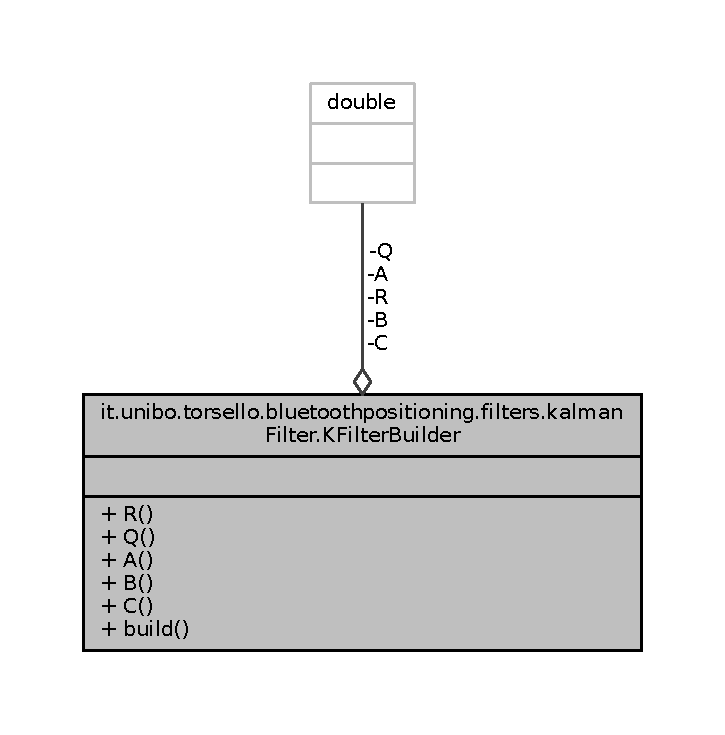
\includegraphics[width=348pt]{classit_1_1unibo_1_1torsello_1_1bluetoothpositioning_1_1filters_1_1kalmanFilter_1_1KFilterBuilder__coll__graph}
\end{center}
\end{figure}
\subsubsection*{Membri pubblici}
\begin{DoxyCompactItemize}
\item 
\hyperlink{classit_1_1unibo_1_1torsello_1_1bluetoothpositioning_1_1filters_1_1kalmanFilter_1_1KFilterBuilder}{K\+Filter\+Builder} \hyperlink{classit_1_1unibo_1_1torsello_1_1bluetoothpositioning_1_1filters_1_1kalmanFilter_1_1KFilterBuilder_a3f4c77bbb350a9f265df4e78aece8b53_a3f4c77bbb350a9f265df4e78aece8b53}{R} (double R)
\item 
\hyperlink{classit_1_1unibo_1_1torsello_1_1bluetoothpositioning_1_1filters_1_1kalmanFilter_1_1KFilterBuilder}{K\+Filter\+Builder} \hyperlink{classit_1_1unibo_1_1torsello_1_1bluetoothpositioning_1_1filters_1_1kalmanFilter_1_1KFilterBuilder_a733c721dce3843456b39f64f54501741_a733c721dce3843456b39f64f54501741}{Q} (double Q)
\item 
\hyperlink{classit_1_1unibo_1_1torsello_1_1bluetoothpositioning_1_1filters_1_1kalmanFilter_1_1KFilterBuilder}{K\+Filter\+Builder} \hyperlink{classit_1_1unibo_1_1torsello_1_1bluetoothpositioning_1_1filters_1_1kalmanFilter_1_1KFilterBuilder_a02fafb90d237636696c0d6a4ace2b2fb_a02fafb90d237636696c0d6a4ace2b2fb}{A} (double A)
\item 
\hyperlink{classit_1_1unibo_1_1torsello_1_1bluetoothpositioning_1_1filters_1_1kalmanFilter_1_1KFilterBuilder}{K\+Filter\+Builder} \hyperlink{classit_1_1unibo_1_1torsello_1_1bluetoothpositioning_1_1filters_1_1kalmanFilter_1_1KFilterBuilder_a50144e5d1e1b7b28534739502e64a103_a50144e5d1e1b7b28534739502e64a103}{B} (double B)
\item 
\hyperlink{classit_1_1unibo_1_1torsello_1_1bluetoothpositioning_1_1filters_1_1kalmanFilter_1_1KFilterBuilder}{K\+Filter\+Builder} \hyperlink{classit_1_1unibo_1_1torsello_1_1bluetoothpositioning_1_1filters_1_1kalmanFilter_1_1KFilterBuilder_a043acfa73226e4a1c4137775d8a40090_a043acfa73226e4a1c4137775d8a40090}{C} (double C)
\item 
\hyperlink{classit_1_1unibo_1_1torsello_1_1bluetoothpositioning_1_1filters_1_1kalmanFilter_1_1KFilter}{K\+Filter} \hyperlink{classit_1_1unibo_1_1torsello_1_1bluetoothpositioning_1_1filters_1_1kalmanFilter_1_1KFilterBuilder_acbd44d335101416f9dc07f31c3e95658_acbd44d335101416f9dc07f31c3e95658}{build} ()
\end{DoxyCompactItemize}
\subsubsection*{Attributi privati}
\begin{DoxyCompactItemize}
\item 
double \hyperlink{classit_1_1unibo_1_1torsello_1_1bluetoothpositioning_1_1filters_1_1kalmanFilter_1_1KFilterBuilder_a524dd60c1b39f891abd153c802a35056_a524dd60c1b39f891abd153c802a35056}{R} = 1
\item 
double \hyperlink{classit_1_1unibo_1_1torsello_1_1bluetoothpositioning_1_1filters_1_1kalmanFilter_1_1KFilterBuilder_a96a8b30ce4611c94928a103f5d03bae2_a96a8b30ce4611c94928a103f5d03bae2}{Q} = 1
\item 
double \hyperlink{classit_1_1unibo_1_1torsello_1_1bluetoothpositioning_1_1filters_1_1kalmanFilter_1_1KFilterBuilder_ad93db15bf28d834081e9fb3df0daad9a_ad93db15bf28d834081e9fb3df0daad9a}{A} = 1
\item 
double \hyperlink{classit_1_1unibo_1_1torsello_1_1bluetoothpositioning_1_1filters_1_1kalmanFilter_1_1KFilterBuilder_a34d29c926b790a773f8f74bfd72e1f56_a34d29c926b790a773f8f74bfd72e1f56}{B} = 0
\item 
double \hyperlink{classit_1_1unibo_1_1torsello_1_1bluetoothpositioning_1_1filters_1_1kalmanFilter_1_1KFilterBuilder_a810bcf844c3b33ba4befbe4ae2698488_a810bcf844c3b33ba4befbe4ae2698488}{C} = 1
\end{DoxyCompactItemize}


\subsubsection{Descrizione dettagliata}
Created by Federico Torsello. \href{mailto:federico.torsello@studio.unibo.it}{\tt federico.\+torsello@studio.\+unibo.\+it} 

Simple builder class for 1-\/dimensional K\+Filter2 filter with predefined 

\subsubsection{Documentazione delle funzioni membro}
\hypertarget{classit_1_1unibo_1_1torsello_1_1bluetoothpositioning_1_1filters_1_1kalmanFilter_1_1KFilterBuilder_a02fafb90d237636696c0d6a4ace2b2fb_a02fafb90d237636696c0d6a4ace2b2fb}{}\label{classit_1_1unibo_1_1torsello_1_1bluetoothpositioning_1_1filters_1_1kalmanFilter_1_1KFilterBuilder_a02fafb90d237636696c0d6a4ace2b2fb_a02fafb90d237636696c0d6a4ace2b2fb} 
\index{it\+::unibo\+::torsello\+::bluetoothpositioning\+::filters\+::kalman\+Filter\+::\+K\+Filter\+Builder@{it\+::unibo\+::torsello\+::bluetoothpositioning\+::filters\+::kalman\+Filter\+::\+K\+Filter\+Builder}!A@{A}}
\index{A@{A}!it\+::unibo\+::torsello\+::bluetoothpositioning\+::filters\+::kalman\+Filter\+::\+K\+Filter\+Builder@{it\+::unibo\+::torsello\+::bluetoothpositioning\+::filters\+::kalman\+Filter\+::\+K\+Filter\+Builder}}
\paragraph{\texorpdfstring{A()}{A()}}
{\footnotesize\ttfamily \hyperlink{classit_1_1unibo_1_1torsello_1_1bluetoothpositioning_1_1filters_1_1kalmanFilter_1_1KFilterBuilder}{K\+Filter\+Builder} it.\+unibo.\+torsello.\+bluetoothpositioning.\+filters.\+kalman\+Filter.\+K\+Filter\+Builder.\+A (\begin{DoxyParamCaption}\item[{double}]{A }\end{DoxyParamCaption})}


\begin{DoxyCode}
27                                       \{
28         this.\hyperlink{classit_1_1unibo_1_1torsello_1_1bluetoothpositioning_1_1filters_1_1kalmanFilter_1_1KFilterBuilder_ad93db15bf28d834081e9fb3df0daad9a_ad93db15bf28d834081e9fb3df0daad9a}{A} = \hyperlink{classit_1_1unibo_1_1torsello_1_1bluetoothpositioning_1_1filters_1_1kalmanFilter_1_1KFilterBuilder_ad93db15bf28d834081e9fb3df0daad9a_ad93db15bf28d834081e9fb3df0daad9a}{A};
29         \textcolor{keywordflow}{return} \textcolor{keyword}{this};
30     \}
\end{DoxyCode}
\hypertarget{classit_1_1unibo_1_1torsello_1_1bluetoothpositioning_1_1filters_1_1kalmanFilter_1_1KFilterBuilder_a50144e5d1e1b7b28534739502e64a103_a50144e5d1e1b7b28534739502e64a103}{}\label{classit_1_1unibo_1_1torsello_1_1bluetoothpositioning_1_1filters_1_1kalmanFilter_1_1KFilterBuilder_a50144e5d1e1b7b28534739502e64a103_a50144e5d1e1b7b28534739502e64a103} 
\index{it\+::unibo\+::torsello\+::bluetoothpositioning\+::filters\+::kalman\+Filter\+::\+K\+Filter\+Builder@{it\+::unibo\+::torsello\+::bluetoothpositioning\+::filters\+::kalman\+Filter\+::\+K\+Filter\+Builder}!B@{B}}
\index{B@{B}!it\+::unibo\+::torsello\+::bluetoothpositioning\+::filters\+::kalman\+Filter\+::\+K\+Filter\+Builder@{it\+::unibo\+::torsello\+::bluetoothpositioning\+::filters\+::kalman\+Filter\+::\+K\+Filter\+Builder}}
\paragraph{\texorpdfstring{B()}{B()}}
{\footnotesize\ttfamily \hyperlink{classit_1_1unibo_1_1torsello_1_1bluetoothpositioning_1_1filters_1_1kalmanFilter_1_1KFilterBuilder}{K\+Filter\+Builder} it.\+unibo.\+torsello.\+bluetoothpositioning.\+filters.\+kalman\+Filter.\+K\+Filter\+Builder.\+B (\begin{DoxyParamCaption}\item[{double}]{B }\end{DoxyParamCaption})}


\begin{DoxyCode}
32                                       \{
33         this.\hyperlink{classit_1_1unibo_1_1torsello_1_1bluetoothpositioning_1_1filters_1_1kalmanFilter_1_1KFilterBuilder_a34d29c926b790a773f8f74bfd72e1f56_a34d29c926b790a773f8f74bfd72e1f56}{B} = \hyperlink{classit_1_1unibo_1_1torsello_1_1bluetoothpositioning_1_1filters_1_1kalmanFilter_1_1KFilterBuilder_a34d29c926b790a773f8f74bfd72e1f56_a34d29c926b790a773f8f74bfd72e1f56}{B};
34         \textcolor{keywordflow}{return} \textcolor{keyword}{this};
35     \}
\end{DoxyCode}
\hypertarget{classit_1_1unibo_1_1torsello_1_1bluetoothpositioning_1_1filters_1_1kalmanFilter_1_1KFilterBuilder_acbd44d335101416f9dc07f31c3e95658_acbd44d335101416f9dc07f31c3e95658}{}\label{classit_1_1unibo_1_1torsello_1_1bluetoothpositioning_1_1filters_1_1kalmanFilter_1_1KFilterBuilder_acbd44d335101416f9dc07f31c3e95658_acbd44d335101416f9dc07f31c3e95658} 
\index{it\+::unibo\+::torsello\+::bluetoothpositioning\+::filters\+::kalman\+Filter\+::\+K\+Filter\+Builder@{it\+::unibo\+::torsello\+::bluetoothpositioning\+::filters\+::kalman\+Filter\+::\+K\+Filter\+Builder}!build@{build}}
\index{build@{build}!it\+::unibo\+::torsello\+::bluetoothpositioning\+::filters\+::kalman\+Filter\+::\+K\+Filter\+Builder@{it\+::unibo\+::torsello\+::bluetoothpositioning\+::filters\+::kalman\+Filter\+::\+K\+Filter\+Builder}}
\paragraph{\texorpdfstring{build()}{build()}}
{\footnotesize\ttfamily \hyperlink{classit_1_1unibo_1_1torsello_1_1bluetoothpositioning_1_1filters_1_1kalmanFilter_1_1KFilter}{K\+Filter} it.\+unibo.\+torsello.\+bluetoothpositioning.\+filters.\+kalman\+Filter.\+K\+Filter\+Builder.\+build (\begin{DoxyParamCaption}{ }\end{DoxyParamCaption})}


\begin{DoxyCode}
42                            \{
43         \textcolor{keywordflow}{return} \textcolor{keyword}{new} KFilter(\hyperlink{classit_1_1unibo_1_1torsello_1_1bluetoothpositioning_1_1filters_1_1kalmanFilter_1_1KFilterBuilder_a524dd60c1b39f891abd153c802a35056_a524dd60c1b39f891abd153c802a35056}{R}, \hyperlink{classit_1_1unibo_1_1torsello_1_1bluetoothpositioning_1_1filters_1_1kalmanFilter_1_1KFilterBuilder_a96a8b30ce4611c94928a103f5d03bae2_a96a8b30ce4611c94928a103f5d03bae2}{Q}, \hyperlink{classit_1_1unibo_1_1torsello_1_1bluetoothpositioning_1_1filters_1_1kalmanFilter_1_1KFilterBuilder_ad93db15bf28d834081e9fb3df0daad9a_ad93db15bf28d834081e9fb3df0daad9a}{A}, \hyperlink{classit_1_1unibo_1_1torsello_1_1bluetoothpositioning_1_1filters_1_1kalmanFilter_1_1KFilterBuilder_a34d29c926b790a773f8f74bfd72e1f56_a34d29c926b790a773f8f74bfd72e1f56}{B}, \hyperlink{classit_1_1unibo_1_1torsello_1_1bluetoothpositioning_1_1filters_1_1kalmanFilter_1_1KFilterBuilder_a810bcf844c3b33ba4befbe4ae2698488_a810bcf844c3b33ba4befbe4ae2698488}{C});
44     \}
\end{DoxyCode}
\hypertarget{classit_1_1unibo_1_1torsello_1_1bluetoothpositioning_1_1filters_1_1kalmanFilter_1_1KFilterBuilder_a043acfa73226e4a1c4137775d8a40090_a043acfa73226e4a1c4137775d8a40090}{}\label{classit_1_1unibo_1_1torsello_1_1bluetoothpositioning_1_1filters_1_1kalmanFilter_1_1KFilterBuilder_a043acfa73226e4a1c4137775d8a40090_a043acfa73226e4a1c4137775d8a40090} 
\index{it\+::unibo\+::torsello\+::bluetoothpositioning\+::filters\+::kalman\+Filter\+::\+K\+Filter\+Builder@{it\+::unibo\+::torsello\+::bluetoothpositioning\+::filters\+::kalman\+Filter\+::\+K\+Filter\+Builder}!C@{C}}
\index{C@{C}!it\+::unibo\+::torsello\+::bluetoothpositioning\+::filters\+::kalman\+Filter\+::\+K\+Filter\+Builder@{it\+::unibo\+::torsello\+::bluetoothpositioning\+::filters\+::kalman\+Filter\+::\+K\+Filter\+Builder}}
\paragraph{\texorpdfstring{C()}{C()}}
{\footnotesize\ttfamily \hyperlink{classit_1_1unibo_1_1torsello_1_1bluetoothpositioning_1_1filters_1_1kalmanFilter_1_1KFilterBuilder}{K\+Filter\+Builder} it.\+unibo.\+torsello.\+bluetoothpositioning.\+filters.\+kalman\+Filter.\+K\+Filter\+Builder.\+C (\begin{DoxyParamCaption}\item[{double}]{C }\end{DoxyParamCaption})}


\begin{DoxyCode}
37                                       \{
38         this.\hyperlink{classit_1_1unibo_1_1torsello_1_1bluetoothpositioning_1_1filters_1_1kalmanFilter_1_1KFilterBuilder_a810bcf844c3b33ba4befbe4ae2698488_a810bcf844c3b33ba4befbe4ae2698488}{C} = \hyperlink{classit_1_1unibo_1_1torsello_1_1bluetoothpositioning_1_1filters_1_1kalmanFilter_1_1KFilterBuilder_a810bcf844c3b33ba4befbe4ae2698488_a810bcf844c3b33ba4befbe4ae2698488}{C};
39         \textcolor{keywordflow}{return} \textcolor{keyword}{this};
40     \}
\end{DoxyCode}
\hypertarget{classit_1_1unibo_1_1torsello_1_1bluetoothpositioning_1_1filters_1_1kalmanFilter_1_1KFilterBuilder_a733c721dce3843456b39f64f54501741_a733c721dce3843456b39f64f54501741}{}\label{classit_1_1unibo_1_1torsello_1_1bluetoothpositioning_1_1filters_1_1kalmanFilter_1_1KFilterBuilder_a733c721dce3843456b39f64f54501741_a733c721dce3843456b39f64f54501741} 
\index{it\+::unibo\+::torsello\+::bluetoothpositioning\+::filters\+::kalman\+Filter\+::\+K\+Filter\+Builder@{it\+::unibo\+::torsello\+::bluetoothpositioning\+::filters\+::kalman\+Filter\+::\+K\+Filter\+Builder}!Q@{Q}}
\index{Q@{Q}!it\+::unibo\+::torsello\+::bluetoothpositioning\+::filters\+::kalman\+Filter\+::\+K\+Filter\+Builder@{it\+::unibo\+::torsello\+::bluetoothpositioning\+::filters\+::kalman\+Filter\+::\+K\+Filter\+Builder}}
\paragraph{\texorpdfstring{Q()}{Q()}}
{\footnotesize\ttfamily \hyperlink{classit_1_1unibo_1_1torsello_1_1bluetoothpositioning_1_1filters_1_1kalmanFilter_1_1KFilterBuilder}{K\+Filter\+Builder} it.\+unibo.\+torsello.\+bluetoothpositioning.\+filters.\+kalman\+Filter.\+K\+Filter\+Builder.\+Q (\begin{DoxyParamCaption}\item[{double}]{Q }\end{DoxyParamCaption})}


\begin{DoxyCode}
22                                       \{
23         this.\hyperlink{classit_1_1unibo_1_1torsello_1_1bluetoothpositioning_1_1filters_1_1kalmanFilter_1_1KFilterBuilder_a96a8b30ce4611c94928a103f5d03bae2_a96a8b30ce4611c94928a103f5d03bae2}{Q} = \hyperlink{classit_1_1unibo_1_1torsello_1_1bluetoothpositioning_1_1filters_1_1kalmanFilter_1_1KFilterBuilder_a96a8b30ce4611c94928a103f5d03bae2_a96a8b30ce4611c94928a103f5d03bae2}{Q};
24         \textcolor{keywordflow}{return} \textcolor{keyword}{this};
25     \}
\end{DoxyCode}
\hypertarget{classit_1_1unibo_1_1torsello_1_1bluetoothpositioning_1_1filters_1_1kalmanFilter_1_1KFilterBuilder_a3f4c77bbb350a9f265df4e78aece8b53_a3f4c77bbb350a9f265df4e78aece8b53}{}\label{classit_1_1unibo_1_1torsello_1_1bluetoothpositioning_1_1filters_1_1kalmanFilter_1_1KFilterBuilder_a3f4c77bbb350a9f265df4e78aece8b53_a3f4c77bbb350a9f265df4e78aece8b53} 
\index{it\+::unibo\+::torsello\+::bluetoothpositioning\+::filters\+::kalman\+Filter\+::\+K\+Filter\+Builder@{it\+::unibo\+::torsello\+::bluetoothpositioning\+::filters\+::kalman\+Filter\+::\+K\+Filter\+Builder}!R@{R}}
\index{R@{R}!it\+::unibo\+::torsello\+::bluetoothpositioning\+::filters\+::kalman\+Filter\+::\+K\+Filter\+Builder@{it\+::unibo\+::torsello\+::bluetoothpositioning\+::filters\+::kalman\+Filter\+::\+K\+Filter\+Builder}}
\paragraph{\texorpdfstring{R()}{R()}}
{\footnotesize\ttfamily \hyperlink{classit_1_1unibo_1_1torsello_1_1bluetoothpositioning_1_1filters_1_1kalmanFilter_1_1KFilterBuilder}{K\+Filter\+Builder} it.\+unibo.\+torsello.\+bluetoothpositioning.\+filters.\+kalman\+Filter.\+K\+Filter\+Builder.\+R (\begin{DoxyParamCaption}\item[{double}]{R }\end{DoxyParamCaption})}


\begin{DoxyCode}
17                                       \{
18         this.\hyperlink{classit_1_1unibo_1_1torsello_1_1bluetoothpositioning_1_1filters_1_1kalmanFilter_1_1KFilterBuilder_a524dd60c1b39f891abd153c802a35056_a524dd60c1b39f891abd153c802a35056}{R} = \hyperlink{classit_1_1unibo_1_1torsello_1_1bluetoothpositioning_1_1filters_1_1kalmanFilter_1_1KFilterBuilder_a524dd60c1b39f891abd153c802a35056_a524dd60c1b39f891abd153c802a35056}{R};
19         \textcolor{keywordflow}{return} \textcolor{keyword}{this};
20     \}
\end{DoxyCode}


\subsubsection{Documentazione dei membri dato}
\hypertarget{classit_1_1unibo_1_1torsello_1_1bluetoothpositioning_1_1filters_1_1kalmanFilter_1_1KFilterBuilder_ad93db15bf28d834081e9fb3df0daad9a_ad93db15bf28d834081e9fb3df0daad9a}{}\label{classit_1_1unibo_1_1torsello_1_1bluetoothpositioning_1_1filters_1_1kalmanFilter_1_1KFilterBuilder_ad93db15bf28d834081e9fb3df0daad9a_ad93db15bf28d834081e9fb3df0daad9a} 
\index{it\+::unibo\+::torsello\+::bluetoothpositioning\+::filters\+::kalman\+Filter\+::\+K\+Filter\+Builder@{it\+::unibo\+::torsello\+::bluetoothpositioning\+::filters\+::kalman\+Filter\+::\+K\+Filter\+Builder}!A@{A}}
\index{A@{A}!it\+::unibo\+::torsello\+::bluetoothpositioning\+::filters\+::kalman\+Filter\+::\+K\+Filter\+Builder@{it\+::unibo\+::torsello\+::bluetoothpositioning\+::filters\+::kalman\+Filter\+::\+K\+Filter\+Builder}}
\paragraph{\texorpdfstring{A}{A}}
{\footnotesize\ttfamily double it.\+unibo.\+torsello.\+bluetoothpositioning.\+filters.\+kalman\+Filter.\+K\+Filter\+Builder.\+A = 1\hspace{0.3cm}{\ttfamily [private]}}

\hypertarget{classit_1_1unibo_1_1torsello_1_1bluetoothpositioning_1_1filters_1_1kalmanFilter_1_1KFilterBuilder_a34d29c926b790a773f8f74bfd72e1f56_a34d29c926b790a773f8f74bfd72e1f56}{}\label{classit_1_1unibo_1_1torsello_1_1bluetoothpositioning_1_1filters_1_1kalmanFilter_1_1KFilterBuilder_a34d29c926b790a773f8f74bfd72e1f56_a34d29c926b790a773f8f74bfd72e1f56} 
\index{it\+::unibo\+::torsello\+::bluetoothpositioning\+::filters\+::kalman\+Filter\+::\+K\+Filter\+Builder@{it\+::unibo\+::torsello\+::bluetoothpositioning\+::filters\+::kalman\+Filter\+::\+K\+Filter\+Builder}!B@{B}}
\index{B@{B}!it\+::unibo\+::torsello\+::bluetoothpositioning\+::filters\+::kalman\+Filter\+::\+K\+Filter\+Builder@{it\+::unibo\+::torsello\+::bluetoothpositioning\+::filters\+::kalman\+Filter\+::\+K\+Filter\+Builder}}
\paragraph{\texorpdfstring{B}{B}}
{\footnotesize\ttfamily double it.\+unibo.\+torsello.\+bluetoothpositioning.\+filters.\+kalman\+Filter.\+K\+Filter\+Builder.\+B = 0\hspace{0.3cm}{\ttfamily [private]}}

\hypertarget{classit_1_1unibo_1_1torsello_1_1bluetoothpositioning_1_1filters_1_1kalmanFilter_1_1KFilterBuilder_a810bcf844c3b33ba4befbe4ae2698488_a810bcf844c3b33ba4befbe4ae2698488}{}\label{classit_1_1unibo_1_1torsello_1_1bluetoothpositioning_1_1filters_1_1kalmanFilter_1_1KFilterBuilder_a810bcf844c3b33ba4befbe4ae2698488_a810bcf844c3b33ba4befbe4ae2698488} 
\index{it\+::unibo\+::torsello\+::bluetoothpositioning\+::filters\+::kalman\+Filter\+::\+K\+Filter\+Builder@{it\+::unibo\+::torsello\+::bluetoothpositioning\+::filters\+::kalman\+Filter\+::\+K\+Filter\+Builder}!C@{C}}
\index{C@{C}!it\+::unibo\+::torsello\+::bluetoothpositioning\+::filters\+::kalman\+Filter\+::\+K\+Filter\+Builder@{it\+::unibo\+::torsello\+::bluetoothpositioning\+::filters\+::kalman\+Filter\+::\+K\+Filter\+Builder}}
\paragraph{\texorpdfstring{C}{C}}
{\footnotesize\ttfamily double it.\+unibo.\+torsello.\+bluetoothpositioning.\+filters.\+kalman\+Filter.\+K\+Filter\+Builder.\+C = 1\hspace{0.3cm}{\ttfamily [private]}}

\hypertarget{classit_1_1unibo_1_1torsello_1_1bluetoothpositioning_1_1filters_1_1kalmanFilter_1_1KFilterBuilder_a96a8b30ce4611c94928a103f5d03bae2_a96a8b30ce4611c94928a103f5d03bae2}{}\label{classit_1_1unibo_1_1torsello_1_1bluetoothpositioning_1_1filters_1_1kalmanFilter_1_1KFilterBuilder_a96a8b30ce4611c94928a103f5d03bae2_a96a8b30ce4611c94928a103f5d03bae2} 
\index{it\+::unibo\+::torsello\+::bluetoothpositioning\+::filters\+::kalman\+Filter\+::\+K\+Filter\+Builder@{it\+::unibo\+::torsello\+::bluetoothpositioning\+::filters\+::kalman\+Filter\+::\+K\+Filter\+Builder}!Q@{Q}}
\index{Q@{Q}!it\+::unibo\+::torsello\+::bluetoothpositioning\+::filters\+::kalman\+Filter\+::\+K\+Filter\+Builder@{it\+::unibo\+::torsello\+::bluetoothpositioning\+::filters\+::kalman\+Filter\+::\+K\+Filter\+Builder}}
\paragraph{\texorpdfstring{Q}{Q}}
{\footnotesize\ttfamily double it.\+unibo.\+torsello.\+bluetoothpositioning.\+filters.\+kalman\+Filter.\+K\+Filter\+Builder.\+Q = 1\hspace{0.3cm}{\ttfamily [private]}}

\hypertarget{classit_1_1unibo_1_1torsello_1_1bluetoothpositioning_1_1filters_1_1kalmanFilter_1_1KFilterBuilder_a524dd60c1b39f891abd153c802a35056_a524dd60c1b39f891abd153c802a35056}{}\label{classit_1_1unibo_1_1torsello_1_1bluetoothpositioning_1_1filters_1_1kalmanFilter_1_1KFilterBuilder_a524dd60c1b39f891abd153c802a35056_a524dd60c1b39f891abd153c802a35056} 
\index{it\+::unibo\+::torsello\+::bluetoothpositioning\+::filters\+::kalman\+Filter\+::\+K\+Filter\+Builder@{it\+::unibo\+::torsello\+::bluetoothpositioning\+::filters\+::kalman\+Filter\+::\+K\+Filter\+Builder}!R@{R}}
\index{R@{R}!it\+::unibo\+::torsello\+::bluetoothpositioning\+::filters\+::kalman\+Filter\+::\+K\+Filter\+Builder@{it\+::unibo\+::torsello\+::bluetoothpositioning\+::filters\+::kalman\+Filter\+::\+K\+Filter\+Builder}}
\paragraph{\texorpdfstring{R}{R}}
{\footnotesize\ttfamily double it.\+unibo.\+torsello.\+bluetoothpositioning.\+filters.\+kalman\+Filter.\+K\+Filter\+Builder.\+R = 1\hspace{0.3cm}{\ttfamily [private]}}



La documentazione per questa classe è stata generata a partire dal seguente file\+:\begin{DoxyCompactItemize}
\item 
\hyperlink{KFilterBuilder_8java}{K\+Filter\+Builder.\+java}\end{DoxyCompactItemize}

\hypertarget{classit_1_1unibo_1_1torsello_1_1bluetoothpositioning_1_1constant_1_1KFilterConstants}{}\subsection{Riferimenti per la classe it.\+unibo.\+torsello.\+bluetoothpositioning.\+constant.\+K\+Filter\+Constants}
\label{classit_1_1unibo_1_1torsello_1_1bluetoothpositioning_1_1constant_1_1KFilterConstants}\index{it.\+unibo.\+torsello.\+bluetoothpositioning.\+constant.\+K\+Filter\+Constants@{it.\+unibo.\+torsello.\+bluetoothpositioning.\+constant.\+K\+Filter\+Constants}}


Diagramma di collaborazione per it.\+unibo.\+torsello.\+bluetoothpositioning.\+constant.\+K\+Filter\+Constants\+:
\nopagebreak
\begin{figure}[H]
\begin{center}
\leavevmode
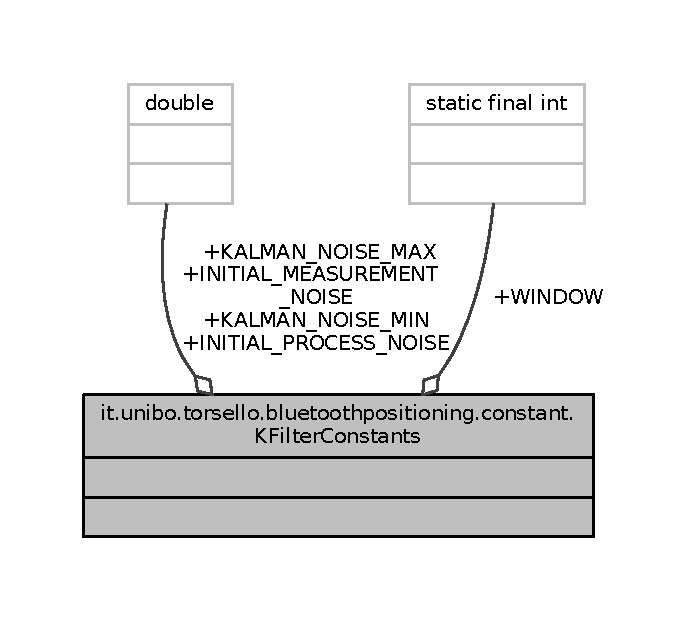
\includegraphics[width=332pt]{classit_1_1unibo_1_1torsello_1_1bluetoothpositioning_1_1constant_1_1KFilterConstants__coll__graph}
\end{center}
\end{figure}
\subsubsection*{Attributi pubblici statici}
\begin{DoxyCompactItemize}
\item 
static final double \hyperlink{classit_1_1unibo_1_1torsello_1_1bluetoothpositioning_1_1constant_1_1KFilterConstants_a8c2adefc8bfb7c419ecfbe3b7ce65112_a8c2adefc8bfb7c419ecfbe3b7ce65112}{K\+A\+L\+M\+A\+N\+\_\+\+N\+O\+I\+S\+E\+\_\+\+M\+IN} = 0D
\item 
static final double \hyperlink{classit_1_1unibo_1_1torsello_1_1bluetoothpositioning_1_1constant_1_1KFilterConstants_aaaf950270c408cc26a79103a56b211cf_aaaf950270c408cc26a79103a56b211cf}{K\+A\+L\+M\+A\+N\+\_\+\+N\+O\+I\+S\+E\+\_\+\+M\+AX} = 5D
\item 
static final double \hyperlink{classit_1_1unibo_1_1torsello_1_1bluetoothpositioning_1_1constant_1_1KFilterConstants_a4604515ac01c25cfabb53248942a00bb_a4604515ac01c25cfabb53248942a00bb}{I\+N\+I\+T\+I\+A\+L\+\_\+\+P\+R\+O\+C\+E\+S\+S\+\_\+\+N\+O\+I\+SE} = 5D
\item 
static final double \hyperlink{classit_1_1unibo_1_1torsello_1_1bluetoothpositioning_1_1constant_1_1KFilterConstants_a5fa646024e9357b089f380b9293f914f_a5fa646024e9357b089f380b9293f914f}{I\+N\+I\+T\+I\+A\+L\+\_\+\+M\+E\+A\+S\+U\+R\+E\+M\+E\+N\+T\+\_\+\+N\+O\+I\+SE} = 5D
\item 
static final int \hyperlink{classit_1_1unibo_1_1torsello_1_1bluetoothpositioning_1_1constant_1_1KFilterConstants_a3c2618e53ad77fcb50785f62868e4c9c_a3c2618e53ad77fcb50785f62868e4c9c}{W\+I\+N\+D\+OW} = 10
\end{DoxyCompactItemize}


\subsubsection{Descrizione dettagliata}
Created by Federico Torsello. \href{mailto:federico.torsello@studio.unibo.it}{\tt federico.\+torsello@studio.\+unibo.\+it} 

\subsubsection{Documentazione dei membri dato}
\hypertarget{classit_1_1unibo_1_1torsello_1_1bluetoothpositioning_1_1constant_1_1KFilterConstants_a5fa646024e9357b089f380b9293f914f_a5fa646024e9357b089f380b9293f914f}{}\label{classit_1_1unibo_1_1torsello_1_1bluetoothpositioning_1_1constant_1_1KFilterConstants_a5fa646024e9357b089f380b9293f914f_a5fa646024e9357b089f380b9293f914f} 
\index{it\+::unibo\+::torsello\+::bluetoothpositioning\+::constant\+::\+K\+Filter\+Constants@{it\+::unibo\+::torsello\+::bluetoothpositioning\+::constant\+::\+K\+Filter\+Constants}!I\+N\+I\+T\+I\+A\+L\+\_\+\+M\+E\+A\+S\+U\+R\+E\+M\+E\+N\+T\+\_\+\+N\+O\+I\+SE@{I\+N\+I\+T\+I\+A\+L\+\_\+\+M\+E\+A\+S\+U\+R\+E\+M\+E\+N\+T\+\_\+\+N\+O\+I\+SE}}
\index{I\+N\+I\+T\+I\+A\+L\+\_\+\+M\+E\+A\+S\+U\+R\+E\+M\+E\+N\+T\+\_\+\+N\+O\+I\+SE@{I\+N\+I\+T\+I\+A\+L\+\_\+\+M\+E\+A\+S\+U\+R\+E\+M\+E\+N\+T\+\_\+\+N\+O\+I\+SE}!it\+::unibo\+::torsello\+::bluetoothpositioning\+::constant\+::\+K\+Filter\+Constants@{it\+::unibo\+::torsello\+::bluetoothpositioning\+::constant\+::\+K\+Filter\+Constants}}
\paragraph{\texorpdfstring{I\+N\+I\+T\+I\+A\+L\+\_\+\+M\+E\+A\+S\+U\+R\+E\+M\+E\+N\+T\+\_\+\+N\+O\+I\+SE}{INITIAL\_MEASUREMENT\_NOISE}}
{\footnotesize\ttfamily final double it.\+unibo.\+torsello.\+bluetoothpositioning.\+constant.\+K\+Filter\+Constants.\+I\+N\+I\+T\+I\+A\+L\+\_\+\+M\+E\+A\+S\+U\+R\+E\+M\+E\+N\+T\+\_\+\+N\+O\+I\+SE = 5D\hspace{0.3cm}{\ttfamily [static]}}

\hypertarget{classit_1_1unibo_1_1torsello_1_1bluetoothpositioning_1_1constant_1_1KFilterConstants_a4604515ac01c25cfabb53248942a00bb_a4604515ac01c25cfabb53248942a00bb}{}\label{classit_1_1unibo_1_1torsello_1_1bluetoothpositioning_1_1constant_1_1KFilterConstants_a4604515ac01c25cfabb53248942a00bb_a4604515ac01c25cfabb53248942a00bb} 
\index{it\+::unibo\+::torsello\+::bluetoothpositioning\+::constant\+::\+K\+Filter\+Constants@{it\+::unibo\+::torsello\+::bluetoothpositioning\+::constant\+::\+K\+Filter\+Constants}!I\+N\+I\+T\+I\+A\+L\+\_\+\+P\+R\+O\+C\+E\+S\+S\+\_\+\+N\+O\+I\+SE@{I\+N\+I\+T\+I\+A\+L\+\_\+\+P\+R\+O\+C\+E\+S\+S\+\_\+\+N\+O\+I\+SE}}
\index{I\+N\+I\+T\+I\+A\+L\+\_\+\+P\+R\+O\+C\+E\+S\+S\+\_\+\+N\+O\+I\+SE@{I\+N\+I\+T\+I\+A\+L\+\_\+\+P\+R\+O\+C\+E\+S\+S\+\_\+\+N\+O\+I\+SE}!it\+::unibo\+::torsello\+::bluetoothpositioning\+::constant\+::\+K\+Filter\+Constants@{it\+::unibo\+::torsello\+::bluetoothpositioning\+::constant\+::\+K\+Filter\+Constants}}
\paragraph{\texorpdfstring{I\+N\+I\+T\+I\+A\+L\+\_\+\+P\+R\+O\+C\+E\+S\+S\+\_\+\+N\+O\+I\+SE}{INITIAL\_PROCESS\_NOISE}}
{\footnotesize\ttfamily final double it.\+unibo.\+torsello.\+bluetoothpositioning.\+constant.\+K\+Filter\+Constants.\+I\+N\+I\+T\+I\+A\+L\+\_\+\+P\+R\+O\+C\+E\+S\+S\+\_\+\+N\+O\+I\+SE = 5D\hspace{0.3cm}{\ttfamily [static]}}

\hypertarget{classit_1_1unibo_1_1torsello_1_1bluetoothpositioning_1_1constant_1_1KFilterConstants_aaaf950270c408cc26a79103a56b211cf_aaaf950270c408cc26a79103a56b211cf}{}\label{classit_1_1unibo_1_1torsello_1_1bluetoothpositioning_1_1constant_1_1KFilterConstants_aaaf950270c408cc26a79103a56b211cf_aaaf950270c408cc26a79103a56b211cf} 
\index{it\+::unibo\+::torsello\+::bluetoothpositioning\+::constant\+::\+K\+Filter\+Constants@{it\+::unibo\+::torsello\+::bluetoothpositioning\+::constant\+::\+K\+Filter\+Constants}!K\+A\+L\+M\+A\+N\+\_\+\+N\+O\+I\+S\+E\+\_\+\+M\+AX@{K\+A\+L\+M\+A\+N\+\_\+\+N\+O\+I\+S\+E\+\_\+\+M\+AX}}
\index{K\+A\+L\+M\+A\+N\+\_\+\+N\+O\+I\+S\+E\+\_\+\+M\+AX@{K\+A\+L\+M\+A\+N\+\_\+\+N\+O\+I\+S\+E\+\_\+\+M\+AX}!it\+::unibo\+::torsello\+::bluetoothpositioning\+::constant\+::\+K\+Filter\+Constants@{it\+::unibo\+::torsello\+::bluetoothpositioning\+::constant\+::\+K\+Filter\+Constants}}
\paragraph{\texorpdfstring{K\+A\+L\+M\+A\+N\+\_\+\+N\+O\+I\+S\+E\+\_\+\+M\+AX}{KALMAN\_NOISE\_MAX}}
{\footnotesize\ttfamily final double it.\+unibo.\+torsello.\+bluetoothpositioning.\+constant.\+K\+Filter\+Constants.\+K\+A\+L\+M\+A\+N\+\_\+\+N\+O\+I\+S\+E\+\_\+\+M\+AX = 5D\hspace{0.3cm}{\ttfamily [static]}}

\hypertarget{classit_1_1unibo_1_1torsello_1_1bluetoothpositioning_1_1constant_1_1KFilterConstants_a8c2adefc8bfb7c419ecfbe3b7ce65112_a8c2adefc8bfb7c419ecfbe3b7ce65112}{}\label{classit_1_1unibo_1_1torsello_1_1bluetoothpositioning_1_1constant_1_1KFilterConstants_a8c2adefc8bfb7c419ecfbe3b7ce65112_a8c2adefc8bfb7c419ecfbe3b7ce65112} 
\index{it\+::unibo\+::torsello\+::bluetoothpositioning\+::constant\+::\+K\+Filter\+Constants@{it\+::unibo\+::torsello\+::bluetoothpositioning\+::constant\+::\+K\+Filter\+Constants}!K\+A\+L\+M\+A\+N\+\_\+\+N\+O\+I\+S\+E\+\_\+\+M\+IN@{K\+A\+L\+M\+A\+N\+\_\+\+N\+O\+I\+S\+E\+\_\+\+M\+IN}}
\index{K\+A\+L\+M\+A\+N\+\_\+\+N\+O\+I\+S\+E\+\_\+\+M\+IN@{K\+A\+L\+M\+A\+N\+\_\+\+N\+O\+I\+S\+E\+\_\+\+M\+IN}!it\+::unibo\+::torsello\+::bluetoothpositioning\+::constant\+::\+K\+Filter\+Constants@{it\+::unibo\+::torsello\+::bluetoothpositioning\+::constant\+::\+K\+Filter\+Constants}}
\paragraph{\texorpdfstring{K\+A\+L\+M\+A\+N\+\_\+\+N\+O\+I\+S\+E\+\_\+\+M\+IN}{KALMAN\_NOISE\_MIN}}
{\footnotesize\ttfamily final double it.\+unibo.\+torsello.\+bluetoothpositioning.\+constant.\+K\+Filter\+Constants.\+K\+A\+L\+M\+A\+N\+\_\+\+N\+O\+I\+S\+E\+\_\+\+M\+IN = 0D\hspace{0.3cm}{\ttfamily [static]}}

\hypertarget{classit_1_1unibo_1_1torsello_1_1bluetoothpositioning_1_1constant_1_1KFilterConstants_a3c2618e53ad77fcb50785f62868e4c9c_a3c2618e53ad77fcb50785f62868e4c9c}{}\label{classit_1_1unibo_1_1torsello_1_1bluetoothpositioning_1_1constant_1_1KFilterConstants_a3c2618e53ad77fcb50785f62868e4c9c_a3c2618e53ad77fcb50785f62868e4c9c} 
\index{it\+::unibo\+::torsello\+::bluetoothpositioning\+::constant\+::\+K\+Filter\+Constants@{it\+::unibo\+::torsello\+::bluetoothpositioning\+::constant\+::\+K\+Filter\+Constants}!W\+I\+N\+D\+OW@{W\+I\+N\+D\+OW}}
\index{W\+I\+N\+D\+OW@{W\+I\+N\+D\+OW}!it\+::unibo\+::torsello\+::bluetoothpositioning\+::constant\+::\+K\+Filter\+Constants@{it\+::unibo\+::torsello\+::bluetoothpositioning\+::constant\+::\+K\+Filter\+Constants}}
\paragraph{\texorpdfstring{W\+I\+N\+D\+OW}{WINDOW}}
{\footnotesize\ttfamily final int it.\+unibo.\+torsello.\+bluetoothpositioning.\+constant.\+K\+Filter\+Constants.\+W\+I\+N\+D\+OW = 10\hspace{0.3cm}{\ttfamily [static]}}



La documentazione per questa classe è stata generata a partire dal seguente file\+:\begin{DoxyCompactItemize}
\item 
\hyperlink{KFilterConstants_8java}{K\+Filter\+Constants.\+java}\end{DoxyCompactItemize}

\hypertarget{classit_1_1unibo_1_1torsello_1_1bluetoothpositioning_1_1activities_1_1MainActivity}{}\subsection{Riferimenti per la classe it.\+unibo.\+torsello.\+bluetoothpositioning.\+activities.\+Main\+Activity}
\label{classit_1_1unibo_1_1torsello_1_1bluetoothpositioning_1_1activities_1_1MainActivity}\index{it.\+unibo.\+torsello.\+bluetoothpositioning.\+activities.\+Main\+Activity@{it.\+unibo.\+torsello.\+bluetoothpositioning.\+activities.\+Main\+Activity}}


Diagramma delle classi per it.\+unibo.\+torsello.\+bluetoothpositioning.\+activities.\+Main\+Activity
\nopagebreak
\begin{figure}[H]
\begin{center}
\leavevmode
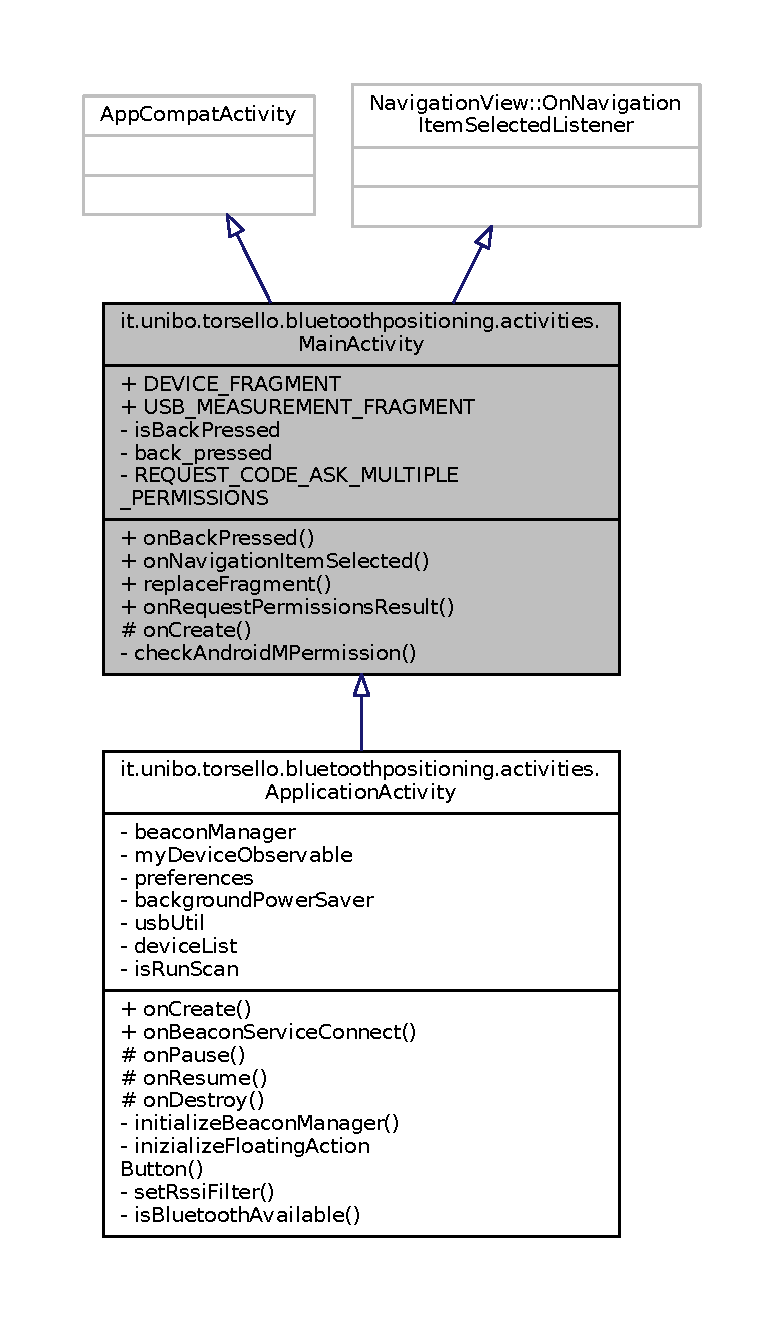
\includegraphics[height=550pt]{classit_1_1unibo_1_1torsello_1_1bluetoothpositioning_1_1activities_1_1MainActivity__inherit__graph}
\end{center}
\end{figure}


Diagramma di collaborazione per it.\+unibo.\+torsello.\+bluetoothpositioning.\+activities.\+Main\+Activity\+:
\nopagebreak
\begin{figure}[H]
\begin{center}
\leavevmode
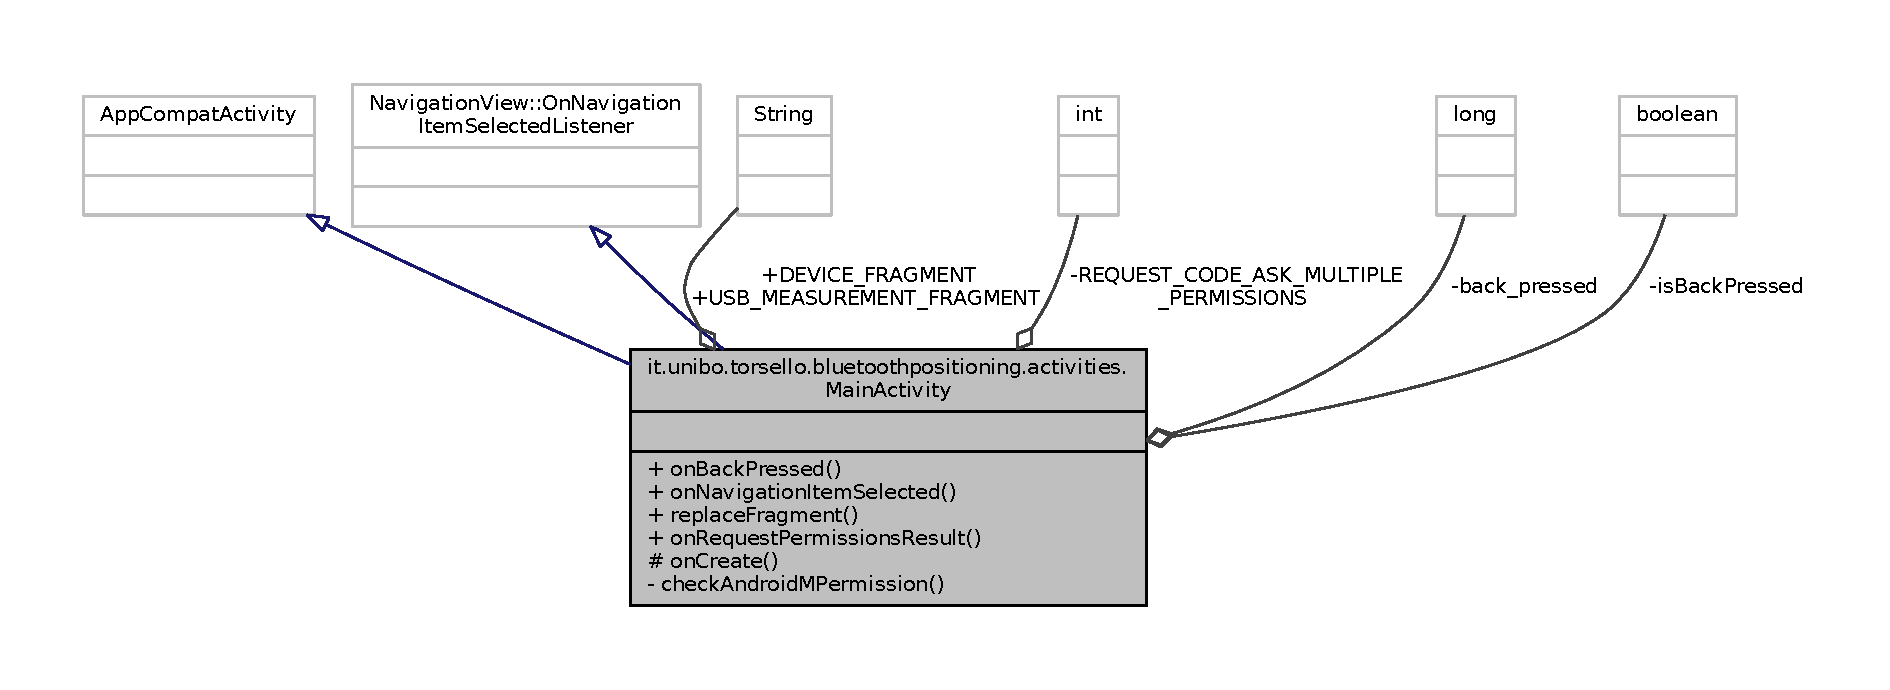
\includegraphics[width=350pt]{classit_1_1unibo_1_1torsello_1_1bluetoothpositioning_1_1activities_1_1MainActivity__coll__graph}
\end{center}
\end{figure}
\subsubsection*{Membri pubblici}
\begin{DoxyCompactItemize}
\item 
void \hyperlink{classit_1_1unibo_1_1torsello_1_1bluetoothpositioning_1_1activities_1_1MainActivity_ab0010b6d3fe518fabfea843626d7b5f1_ab0010b6d3fe518fabfea843626d7b5f1}{on\+Back\+Pressed} ()
\item 
boolean \hyperlink{classit_1_1unibo_1_1torsello_1_1bluetoothpositioning_1_1activities_1_1MainActivity_a7cfc0a2ee94c12afaac3b7472eeb75b7_a7cfc0a2ee94c12afaac3b7472eeb75b7}{on\+Navigation\+Item\+Selected} (Menu\+Item item)
\item 
void \hyperlink{classit_1_1unibo_1_1torsello_1_1bluetoothpositioning_1_1activities_1_1MainActivity_a98db4478d28cd91118138d0b652ceb2c_a98db4478d28cd91118138d0b652ceb2c}{replace\+Fragment} (String frag\+Tag)
\item 
void \hyperlink{classit_1_1unibo_1_1torsello_1_1bluetoothpositioning_1_1activities_1_1MainActivity_a81d7581dfa4998b2ad8139f103328cf9_a81d7581dfa4998b2ad8139f103328cf9}{on\+Request\+Permissions\+Result} (int request\+Code, @Non\+Null String permissions\mbox{[}$\,$\mbox{]}, @Non\+Null int\mbox{[}$\,$\mbox{]} grant\+Results)
\end{DoxyCompactItemize}
\subsubsection*{Attributi pubblici statici}
\begin{DoxyCompactItemize}
\item 
static final String \hyperlink{classit_1_1unibo_1_1torsello_1_1bluetoothpositioning_1_1activities_1_1MainActivity_a2f77c0245ac2525dc58905e38e1817d1_a2f77c0245ac2525dc58905e38e1817d1}{D\+E\+V\+I\+C\+E\+\_\+\+F\+R\+A\+G\+M\+E\+NT} = \char`\"{}device\char`\"{}
\item 
static final String \hyperlink{classit_1_1unibo_1_1torsello_1_1bluetoothpositioning_1_1activities_1_1MainActivity_a64bac06e6db556ba1e36c8773e61137b_a64bac06e6db556ba1e36c8773e61137b}{U\+S\+B\+\_\+\+M\+E\+A\+S\+U\+R\+E\+M\+E\+N\+T\+\_\+\+F\+R\+A\+G\+M\+E\+NT} = \char`\"{}usb measurement\char`\"{}
\end{DoxyCompactItemize}
\subsubsection*{Membri protetti}
\begin{DoxyCompactItemize}
\item 
void \hyperlink{classit_1_1unibo_1_1torsello_1_1bluetoothpositioning_1_1activities_1_1MainActivity_a8ffa5fa91fb4ae13a758a12682872a79_a8ffa5fa91fb4ae13a758a12682872a79}{on\+Create} (Bundle saved\+Instance\+State)
\end{DoxyCompactItemize}
\subsubsection*{Membri privati}
\begin{DoxyCompactItemize}
\item 
void \hyperlink{classit_1_1unibo_1_1torsello_1_1bluetoothpositioning_1_1activities_1_1MainActivity_ab762aac3d11f5b0ccc6042a140804d5d_ab762aac3d11f5b0ccc6042a140804d5d}{check\+Android\+M\+Permission} ()
\end{DoxyCompactItemize}
\subsubsection*{Attributi privati}
\begin{DoxyCompactItemize}
\item 
final String \hyperlink{classit_1_1unibo_1_1torsello_1_1bluetoothpositioning_1_1activities_1_1MainActivity_ab45ec7669a9285270b5dc817334762b3_ab45ec7669a9285270b5dc817334762b3}{T\+A\+G\+\_\+\+C\+L\+A\+SS} = get\+Class().get\+Simple\+Name()
\item 
boolean \hyperlink{classit_1_1unibo_1_1torsello_1_1bluetoothpositioning_1_1activities_1_1MainActivity_a73d74411ec7bb55eb827bb81018174bd_a73d74411ec7bb55eb827bb81018174bd}{is\+Back\+Pressed} = false
\item 
long \hyperlink{classit_1_1unibo_1_1torsello_1_1bluetoothpositioning_1_1activities_1_1MainActivity_a5e1ae38b2bbdcc45f2164fdc393ca495_a5e1ae38b2bbdcc45f2164fdc393ca495}{back\+\_\+pressed}
\item 
final int \hyperlink{classit_1_1unibo_1_1torsello_1_1bluetoothpositioning_1_1activities_1_1MainActivity_a319aed5cdd5724e043302babe5fcfeac_a319aed5cdd5724e043302babe5fcfeac}{R\+E\+Q\+U\+E\+S\+T\+\_\+\+C\+O\+D\+E\+\_\+\+A\+S\+K\+\_\+\+M\+U\+L\+T\+I\+P\+L\+E\+\_\+\+P\+E\+R\+M\+I\+S\+S\+I\+O\+NS} = 124
\end{DoxyCompactItemize}


\subsubsection{Descrizione dettagliata}
Created by Federico Torsello. \href{mailto:federico.torsello@studio.unibo.it}{\tt federico.\+torsello@studio.\+unibo.\+it} 

\subsubsection{Documentazione delle funzioni membro}
\hypertarget{classit_1_1unibo_1_1torsello_1_1bluetoothpositioning_1_1activities_1_1MainActivity_ab762aac3d11f5b0ccc6042a140804d5d_ab762aac3d11f5b0ccc6042a140804d5d}{}\label{classit_1_1unibo_1_1torsello_1_1bluetoothpositioning_1_1activities_1_1MainActivity_ab762aac3d11f5b0ccc6042a140804d5d_ab762aac3d11f5b0ccc6042a140804d5d} 
\index{it\+::unibo\+::torsello\+::bluetoothpositioning\+::activities\+::\+Main\+Activity@{it\+::unibo\+::torsello\+::bluetoothpositioning\+::activities\+::\+Main\+Activity}!check\+Android\+M\+Permission@{check\+Android\+M\+Permission}}
\index{check\+Android\+M\+Permission@{check\+Android\+M\+Permission}!it\+::unibo\+::torsello\+::bluetoothpositioning\+::activities\+::\+Main\+Activity@{it\+::unibo\+::torsello\+::bluetoothpositioning\+::activities\+::\+Main\+Activity}}
\paragraph{\texorpdfstring{check\+Android\+M\+Permission()}{checkAndroidMPermission()}}
{\footnotesize\ttfamily void it.\+unibo.\+torsello.\+bluetoothpositioning.\+activities.\+Main\+Activity.\+check\+Android\+M\+Permission (\begin{DoxyParamCaption}{ }\end{DoxyParamCaption})\hspace{0.3cm}{\ttfamily [private]}}


\begin{DoxyCode}
173                                            \{
174 
175         \textcolor{keywordflow}{if} (Build.VERSION.SDK\_INT >= Build.VERSION\_CODES.M) \{
176             \textcolor{keyword}{final} List<String> permissions = \textcolor{keyword}{new} ArrayList<>();
177 
178             \textcolor{keywordflow}{if} (checkSelfPermission(Manifest.permission.ACCESS\_FINE\_LOCATION)
179                     != PackageManager.PERMISSION\_GRANTED) \{
180                 permissions.add(Manifest.permission.ACCESS\_FINE\_LOCATION);
181             \}
182 
183             \textcolor{keywordflow}{if} (checkSelfPermission(Manifest.permission.ACCESS\_COARSE\_LOCATION)
184                     != PackageManager.PERMISSION\_GRANTED) \{
185                 permissions.add(Manifest.permission.ACCESS\_COARSE\_LOCATION);
186             \}
187 
188             \textcolor{keywordflow}{if} (!permissions.isEmpty()) \{
189                 \textcolor{keyword}{new} AlertDialog.Builder(\textcolor{keyword}{this})
190                         .setTitle(R.string.dialog\_location\_access\_title)
191                         .setMessage(R.string.dialog\_bluetooth\_text)
192                         .setPositiveButton(android.R.string.ok, null)
193                         .setOnDismissListener(\textcolor{keyword}{new} DialogInterface.OnDismissListener() \{
194                             @TargetApi(23)
195                             @Override
196                             \textcolor{keyword}{public} \textcolor{keywordtype}{void} onDismiss(DialogInterface dialog) \{
197                                 requestPermissions(permissions.toArray(\textcolor{keyword}{new} String[permissions.size()]),
198                                         \hyperlink{classit_1_1unibo_1_1torsello_1_1bluetoothpositioning_1_1activities_1_1MainActivity_a319aed5cdd5724e043302babe5fcfeac_a319aed5cdd5724e043302babe5fcfeac}{REQUEST\_CODE\_ASK\_MULTIPLE\_PERMISSIONS}
      );
199                             \}
200 
201                         \}).show();
202             \}
203         \}
204     \}
\end{DoxyCode}
\hypertarget{classit_1_1unibo_1_1torsello_1_1bluetoothpositioning_1_1activities_1_1MainActivity_ab0010b6d3fe518fabfea843626d7b5f1_ab0010b6d3fe518fabfea843626d7b5f1}{}\label{classit_1_1unibo_1_1torsello_1_1bluetoothpositioning_1_1activities_1_1MainActivity_ab0010b6d3fe518fabfea843626d7b5f1_ab0010b6d3fe518fabfea843626d7b5f1} 
\index{it\+::unibo\+::torsello\+::bluetoothpositioning\+::activities\+::\+Main\+Activity@{it\+::unibo\+::torsello\+::bluetoothpositioning\+::activities\+::\+Main\+Activity}!on\+Back\+Pressed@{on\+Back\+Pressed}}
\index{on\+Back\+Pressed@{on\+Back\+Pressed}!it\+::unibo\+::torsello\+::bluetoothpositioning\+::activities\+::\+Main\+Activity@{it\+::unibo\+::torsello\+::bluetoothpositioning\+::activities\+::\+Main\+Activity}}
\paragraph{\texorpdfstring{on\+Back\+Pressed()}{onBackPressed()}}
{\footnotesize\ttfamily void it.\+unibo.\+torsello.\+bluetoothpositioning.\+activities.\+Main\+Activity.\+on\+Back\+Pressed (\begin{DoxyParamCaption}{ }\end{DoxyParamCaption})}


\begin{DoxyCode}
70                                 \{
71 
72         DrawerLayout drawer = (DrawerLayout) findViewById(R.id.drawer\_layout);
73         \textcolor{keywordflow}{if} (drawer.isDrawerOpen(GravityCompat.START)) \{
74             drawer.closeDrawer(GravityCompat.START);
75         \} \textcolor{keywordflow}{else} \textcolor{keywordflow}{if} (drawer.isDrawerOpen(GravityCompat.END)) \{
76             drawer.closeDrawer(GravityCompat.END);
77         \} \textcolor{keywordflow}{else} \{
78 
79             \hyperlink{classit_1_1unibo_1_1torsello_1_1bluetoothpositioning_1_1activities_1_1MainActivity_a98db4478d28cd91118138d0b652ceb2c_a98db4478d28cd91118138d0b652ceb2c}{replaceFragment}(\hyperlink{classit_1_1unibo_1_1torsello_1_1bluetoothpositioning_1_1activities_1_1MainActivity_a2f77c0245ac2525dc58905e38e1817d1_a2f77c0245ac2525dc58905e38e1817d1}{DEVICE\_FRAGMENT});
80 
81             \textcolor{keyword}{final} \textcolor{keywordtype}{long} DOUBLE\_PRESS\_INTERVAL = 1500L;
82             \textcolor{keywordflow}{if} (!\hyperlink{classit_1_1unibo_1_1torsello_1_1bluetoothpositioning_1_1activities_1_1MainActivity_a73d74411ec7bb55eb827bb81018174bd_a73d74411ec7bb55eb827bb81018174bd}{isBackPressed} || \hyperlink{classit_1_1unibo_1_1torsello_1_1bluetoothpositioning_1_1activities_1_1MainActivity_a5e1ae38b2bbdcc45f2164fdc393ca495_a5e1ae38b2bbdcc45f2164fdc393ca495}{back\_pressed} + DOUBLE\_PRESS\_INTERVAL <= System.
      currentTimeMillis()) \{
83                 \hyperlink{classit_1_1unibo_1_1torsello_1_1bluetoothpositioning_1_1activities_1_1MainActivity_a73d74411ec7bb55eb827bb81018174bd_a73d74411ec7bb55eb827bb81018174bd}{isBackPressed} = \textcolor{keyword}{true};
84                 FloatingActionButton fab = (FloatingActionButton) findViewById(R.id.fab);
85                 assert fab != null;
86                 Snackbar.make(fab, R.string.snackBar\_exit, Snackbar.LENGTH\_SHORT).show();
87             \} \textcolor{keywordflow}{else} \{
88                 super.finish();
89             \}
90             \hyperlink{classit_1_1unibo_1_1torsello_1_1bluetoothpositioning_1_1activities_1_1MainActivity_a5e1ae38b2bbdcc45f2164fdc393ca495_a5e1ae38b2bbdcc45f2164fdc393ca495}{back\_pressed} = System.currentTimeMillis();
91         \}
92     \}
\end{DoxyCode}
\hypertarget{classit_1_1unibo_1_1torsello_1_1bluetoothpositioning_1_1activities_1_1MainActivity_a8ffa5fa91fb4ae13a758a12682872a79_a8ffa5fa91fb4ae13a758a12682872a79}{}\label{classit_1_1unibo_1_1torsello_1_1bluetoothpositioning_1_1activities_1_1MainActivity_a8ffa5fa91fb4ae13a758a12682872a79_a8ffa5fa91fb4ae13a758a12682872a79} 
\index{it\+::unibo\+::torsello\+::bluetoothpositioning\+::activities\+::\+Main\+Activity@{it\+::unibo\+::torsello\+::bluetoothpositioning\+::activities\+::\+Main\+Activity}!on\+Create@{on\+Create}}
\index{on\+Create@{on\+Create}!it\+::unibo\+::torsello\+::bluetoothpositioning\+::activities\+::\+Main\+Activity@{it\+::unibo\+::torsello\+::bluetoothpositioning\+::activities\+::\+Main\+Activity}}
\paragraph{\texorpdfstring{on\+Create()}{onCreate()}}
{\footnotesize\ttfamily void it.\+unibo.\+torsello.\+bluetoothpositioning.\+activities.\+Main\+Activity.\+on\+Create (\begin{DoxyParamCaption}\item[{Bundle}]{saved\+Instance\+State }\end{DoxyParamCaption})\hspace{0.3cm}{\ttfamily [protected]}}


\begin{DoxyCode}
47                                                        \{
48         super.onCreate(savedInstanceState);
49         setContentView(R.layout.activity\_main);
50 
51         Toolbar toolbar = (Toolbar) findViewById(R.id.toolbar);
52         setSupportActionBar(toolbar);
53 
54         DrawerLayout drawer = (DrawerLayout) findViewById(R.id.drawer\_layout);
55         ActionBarDrawerToggle toggle = \textcolor{keyword}{new} ActionBarDrawerToggle(
56                 \textcolor{keyword}{this}, drawer, toolbar, R.string.navigation\_drawer\_open, R.string.navigation\_drawer\_close);
57         drawer.addDrawerListener(toggle);
58         toggle.syncState();
59 
60         ((NavigationView) findViewById(R.id.nav\_view)).setNavigationItemSelectedListener(\textcolor{keyword}{this});
61 
62         ((NavigationView) findViewById(R.id.nav\_view2)).setNavigationItemSelectedListener(\textcolor{keyword}{this});
63 
64         \hyperlink{classit_1_1unibo_1_1torsello_1_1bluetoothpositioning_1_1activities_1_1MainActivity_a98db4478d28cd91118138d0b652ceb2c_a98db4478d28cd91118138d0b652ceb2c}{replaceFragment}(\hyperlink{classit_1_1unibo_1_1torsello_1_1bluetoothpositioning_1_1activities_1_1MainActivity_a2f77c0245ac2525dc58905e38e1817d1_a2f77c0245ac2525dc58905e38e1817d1}{DEVICE\_FRAGMENT});
65 
66         \hyperlink{classit_1_1unibo_1_1torsello_1_1bluetoothpositioning_1_1activities_1_1MainActivity_ab762aac3d11f5b0ccc6042a140804d5d_ab762aac3d11f5b0ccc6042a140804d5d}{checkAndroidMPermission}();
67     \}
\end{DoxyCode}
\hypertarget{classit_1_1unibo_1_1torsello_1_1bluetoothpositioning_1_1activities_1_1MainActivity_a7cfc0a2ee94c12afaac3b7472eeb75b7_a7cfc0a2ee94c12afaac3b7472eeb75b7}{}\label{classit_1_1unibo_1_1torsello_1_1bluetoothpositioning_1_1activities_1_1MainActivity_a7cfc0a2ee94c12afaac3b7472eeb75b7_a7cfc0a2ee94c12afaac3b7472eeb75b7} 
\index{it\+::unibo\+::torsello\+::bluetoothpositioning\+::activities\+::\+Main\+Activity@{it\+::unibo\+::torsello\+::bluetoothpositioning\+::activities\+::\+Main\+Activity}!on\+Navigation\+Item\+Selected@{on\+Navigation\+Item\+Selected}}
\index{on\+Navigation\+Item\+Selected@{on\+Navigation\+Item\+Selected}!it\+::unibo\+::torsello\+::bluetoothpositioning\+::activities\+::\+Main\+Activity@{it\+::unibo\+::torsello\+::bluetoothpositioning\+::activities\+::\+Main\+Activity}}
\paragraph{\texorpdfstring{on\+Navigation\+Item\+Selected()}{onNavigationItemSelected()}}
{\footnotesize\ttfamily boolean it.\+unibo.\+torsello.\+bluetoothpositioning.\+activities.\+Main\+Activity.\+on\+Navigation\+Item\+Selected (\begin{DoxyParamCaption}\item[{Menu\+Item}]{item }\end{DoxyParamCaption})}


\begin{DoxyCode}
96                                                            \{
97 
98         DrawerLayout drawer = (DrawerLayout) findViewById(R.id.drawer\_layout);
99 
100         \textcolor{comment}{// Handle navigation view item clicks here.}
101         \textcolor{keywordflow}{switch} (item.getItemId()) \{
102             \textcolor{keywordflow}{case} R.id.nav\_home:
103                 \hyperlink{classit_1_1unibo_1_1torsello_1_1bluetoothpositioning_1_1activities_1_1MainActivity_a98db4478d28cd91118138d0b652ceb2c_a98db4478d28cd91118138d0b652ceb2c}{replaceFragment}(\hyperlink{classit_1_1unibo_1_1torsello_1_1bluetoothpositioning_1_1activities_1_1MainActivity_a2f77c0245ac2525dc58905e38e1817d1_a2f77c0245ac2525dc58905e38e1817d1}{DEVICE\_FRAGMENT});
104                 \textcolor{keywordflow}{break};
105             \textcolor{keywordflow}{case} R.id.nav\_settings:
106                 drawer.openDrawer(GravityCompat.END);
107                 \textcolor{keywordflow}{break};
108             \textcolor{keywordflow}{case} R.id.nav\_measurement:
109                 \hyperlink{classit_1_1unibo_1_1torsello_1_1bluetoothpositioning_1_1activities_1_1MainActivity_a98db4478d28cd91118138d0b652ceb2c_a98db4478d28cd91118138d0b652ceb2c}{replaceFragment}(\hyperlink{classit_1_1unibo_1_1torsello_1_1bluetoothpositioning_1_1activities_1_1MainActivity_a64bac06e6db556ba1e36c8773e61137b_a64bac06e6db556ba1e36c8773e61137b}{USB\_MEASUREMENT\_FRAGMENT});
110                 \textcolor{keywordflow}{break};
111 \textcolor{comment}{//            case R.id.nav\_share:}
112 \textcolor{comment}{//                fragment = CamTestFragment.newInstance();}
113 \textcolor{comment}{//                break;}
114 \textcolor{comment}{//            case R.id.nav\_send:}
115 \textcolor{comment}{//                fragment = ViewPagerFragment.newInstance(getFragments());}
116 \textcolor{comment}{//                break;}
117         \}
118 
119         \textcolor{keywordflow}{if} (drawer.isDrawerOpen(GravityCompat.START)) \{
120             drawer.closeDrawer(GravityCompat.START);
121         \}
122 
123         \textcolor{keywordflow}{return} \textcolor{keyword}{true};
124     \}
\end{DoxyCode}
\hypertarget{classit_1_1unibo_1_1torsello_1_1bluetoothpositioning_1_1activities_1_1MainActivity_a81d7581dfa4998b2ad8139f103328cf9_a81d7581dfa4998b2ad8139f103328cf9}{}\label{classit_1_1unibo_1_1torsello_1_1bluetoothpositioning_1_1activities_1_1MainActivity_a81d7581dfa4998b2ad8139f103328cf9_a81d7581dfa4998b2ad8139f103328cf9} 
\index{it\+::unibo\+::torsello\+::bluetoothpositioning\+::activities\+::\+Main\+Activity@{it\+::unibo\+::torsello\+::bluetoothpositioning\+::activities\+::\+Main\+Activity}!on\+Request\+Permissions\+Result@{on\+Request\+Permissions\+Result}}
\index{on\+Request\+Permissions\+Result@{on\+Request\+Permissions\+Result}!it\+::unibo\+::torsello\+::bluetoothpositioning\+::activities\+::\+Main\+Activity@{it\+::unibo\+::torsello\+::bluetoothpositioning\+::activities\+::\+Main\+Activity}}
\paragraph{\texorpdfstring{on\+Request\+Permissions\+Result()}{onRequestPermissionsResult()}}
{\footnotesize\ttfamily void it.\+unibo.\+torsello.\+bluetoothpositioning.\+activities.\+Main\+Activity.\+on\+Request\+Permissions\+Result (\begin{DoxyParamCaption}\item[{int}]{request\+Code,  }\item[{@Non\+Null String}]{permissions\mbox{[}$\,$\mbox{]},  }\item[{@Non\+Null int \mbox{[}$\,$\mbox{]}}]{grant\+Results }\end{DoxyParamCaption})}


\begin{DoxyCode}
146                                                                         \{
147         \textcolor{keywordflow}{switch} (requestCode) \{
148             \textcolor{keywordflow}{case} \hyperlink{classit_1_1unibo_1_1torsello_1_1bluetoothpositioning_1_1activities_1_1MainActivity_a319aed5cdd5724e043302babe5fcfeac_a319aed5cdd5724e043302babe5fcfeac}{REQUEST\_CODE\_ASK\_MULTIPLE\_PERMISSIONS}:
149                 \textcolor{keywordflow}{for} (\textcolor{keywordtype}{int} i = 0; i < permissions.length; i++) \{
150                     \textcolor{keywordflow}{if} (grantResults[i] == PackageManager.PERMISSION\_GRANTED) \{
151 \textcolor{comment}{//                        Log.d(TAG\_CLASS, "Permission Granted: " + permissions[i]);}
152                     \} \textcolor{keywordflow}{else} \textcolor{keywordflow}{if} (grantResults[i] == PackageManager.PERMISSION\_DENIED) \{
153 \textcolor{comment}{//                        Log.d(TAG\_CLASS, "Permission Denied: " + permissions[i]);}
154                         \textcolor{keyword}{new} AlertDialog.Builder(\textcolor{keyword}{this})
155                                 .setTitle(R.string.dialog\_permissions\_location\_access\_title)
156                                 .setMessage(R.string.dialog\_permissions\_location\_access\_text)
157                                 .setPositiveButton(android.R.string.ok, null)
158                                 .setOnDismissListener(\textcolor{keyword}{new} DialogInterface.OnDismissListener() \{
159 
160                                     @Override
161                                     \textcolor{keyword}{public} \textcolor{keywordtype}{void} onDismiss(DialogInterface dialog) \{
162                                     \}
163 
164                                 \}).show();
165                     \}
166                 \}
167                 \textcolor{keywordflow}{break};
168             \textcolor{keywordflow}{default}:
169                 super.onRequestPermissionsResult(requestCode, permissions, grantResults);
170         \}
171     \}
\end{DoxyCode}
\hypertarget{classit_1_1unibo_1_1torsello_1_1bluetoothpositioning_1_1activities_1_1MainActivity_a98db4478d28cd91118138d0b652ceb2c_a98db4478d28cd91118138d0b652ceb2c}{}\label{classit_1_1unibo_1_1torsello_1_1bluetoothpositioning_1_1activities_1_1MainActivity_a98db4478d28cd91118138d0b652ceb2c_a98db4478d28cd91118138d0b652ceb2c} 
\index{it\+::unibo\+::torsello\+::bluetoothpositioning\+::activities\+::\+Main\+Activity@{it\+::unibo\+::torsello\+::bluetoothpositioning\+::activities\+::\+Main\+Activity}!replace\+Fragment@{replace\+Fragment}}
\index{replace\+Fragment@{replace\+Fragment}!it\+::unibo\+::torsello\+::bluetoothpositioning\+::activities\+::\+Main\+Activity@{it\+::unibo\+::torsello\+::bluetoothpositioning\+::activities\+::\+Main\+Activity}}
\paragraph{\texorpdfstring{replace\+Fragment()}{replaceFragment()}}
{\footnotesize\ttfamily void it.\+unibo.\+torsello.\+bluetoothpositioning.\+activities.\+Main\+Activity.\+replace\+Fragment (\begin{DoxyParamCaption}\item[{String}]{frag\+Tag }\end{DoxyParamCaption})}


\begin{DoxyCode}
126                                                 \{
127         Fragment currentFragment = getSupportFragmentManager().findFragmentByTag(fragTag);
128         \textcolor{keywordflow}{switch} (fragTag) \{
129             \textcolor{keywordflow}{case} \hyperlink{classit_1_1unibo_1_1torsello_1_1bluetoothpositioning_1_1activities_1_1MainActivity_a2f77c0245ac2525dc58905e38e1817d1_a2f77c0245ac2525dc58905e38e1817d1}{DEVICE\_FRAGMENT}:
130                 currentFragment = DeviceListFragment.newInstance();
131                 \textcolor{keywordflow}{break};
132             \textcolor{keywordflow}{case} \hyperlink{classit_1_1unibo_1_1torsello_1_1bluetoothpositioning_1_1activities_1_1MainActivity_a64bac06e6db556ba1e36c8773e61137b_a64bac06e6db556ba1e36c8773e61137b}{USB\_MEASUREMENT\_FRAGMENT}:
133                 currentFragment = UsbMeasurementFragment.newInstance();
134                 \textcolor{keywordflow}{break};
135         \}
136 
137         \textcolor{keywordflow}{if} (currentFragment != null) \{
138             getSupportFragmentManager().beginTransaction()
139                     .replace(R.id.contentMainLayout, currentFragment, fragTag)
140                     .commit();
141         \}
142     \}
\end{DoxyCode}


\subsubsection{Documentazione dei membri dato}
\hypertarget{classit_1_1unibo_1_1torsello_1_1bluetoothpositioning_1_1activities_1_1MainActivity_a5e1ae38b2bbdcc45f2164fdc393ca495_a5e1ae38b2bbdcc45f2164fdc393ca495}{}\label{classit_1_1unibo_1_1torsello_1_1bluetoothpositioning_1_1activities_1_1MainActivity_a5e1ae38b2bbdcc45f2164fdc393ca495_a5e1ae38b2bbdcc45f2164fdc393ca495} 
\index{it\+::unibo\+::torsello\+::bluetoothpositioning\+::activities\+::\+Main\+Activity@{it\+::unibo\+::torsello\+::bluetoothpositioning\+::activities\+::\+Main\+Activity}!back\+\_\+pressed@{back\+\_\+pressed}}
\index{back\+\_\+pressed@{back\+\_\+pressed}!it\+::unibo\+::torsello\+::bluetoothpositioning\+::activities\+::\+Main\+Activity@{it\+::unibo\+::torsello\+::bluetoothpositioning\+::activities\+::\+Main\+Activity}}
\paragraph{\texorpdfstring{back\+\_\+pressed}{back\_pressed}}
{\footnotesize\ttfamily long it.\+unibo.\+torsello.\+bluetoothpositioning.\+activities.\+Main\+Activity.\+back\+\_\+pressed\hspace{0.3cm}{\ttfamily [private]}}

\hypertarget{classit_1_1unibo_1_1torsello_1_1bluetoothpositioning_1_1activities_1_1MainActivity_a2f77c0245ac2525dc58905e38e1817d1_a2f77c0245ac2525dc58905e38e1817d1}{}\label{classit_1_1unibo_1_1torsello_1_1bluetoothpositioning_1_1activities_1_1MainActivity_a2f77c0245ac2525dc58905e38e1817d1_a2f77c0245ac2525dc58905e38e1817d1} 
\index{it\+::unibo\+::torsello\+::bluetoothpositioning\+::activities\+::\+Main\+Activity@{it\+::unibo\+::torsello\+::bluetoothpositioning\+::activities\+::\+Main\+Activity}!D\+E\+V\+I\+C\+E\+\_\+\+F\+R\+A\+G\+M\+E\+NT@{D\+E\+V\+I\+C\+E\+\_\+\+F\+R\+A\+G\+M\+E\+NT}}
\index{D\+E\+V\+I\+C\+E\+\_\+\+F\+R\+A\+G\+M\+E\+NT@{D\+E\+V\+I\+C\+E\+\_\+\+F\+R\+A\+G\+M\+E\+NT}!it\+::unibo\+::torsello\+::bluetoothpositioning\+::activities\+::\+Main\+Activity@{it\+::unibo\+::torsello\+::bluetoothpositioning\+::activities\+::\+Main\+Activity}}
\paragraph{\texorpdfstring{D\+E\+V\+I\+C\+E\+\_\+\+F\+R\+A\+G\+M\+E\+NT}{DEVICE\_FRAGMENT}}
{\footnotesize\ttfamily final String it.\+unibo.\+torsello.\+bluetoothpositioning.\+activities.\+Main\+Activity.\+D\+E\+V\+I\+C\+E\+\_\+\+F\+R\+A\+G\+M\+E\+NT = \char`\"{}device\char`\"{}\hspace{0.3cm}{\ttfamily [static]}}

\hypertarget{classit_1_1unibo_1_1torsello_1_1bluetoothpositioning_1_1activities_1_1MainActivity_a73d74411ec7bb55eb827bb81018174bd_a73d74411ec7bb55eb827bb81018174bd}{}\label{classit_1_1unibo_1_1torsello_1_1bluetoothpositioning_1_1activities_1_1MainActivity_a73d74411ec7bb55eb827bb81018174bd_a73d74411ec7bb55eb827bb81018174bd} 
\index{it\+::unibo\+::torsello\+::bluetoothpositioning\+::activities\+::\+Main\+Activity@{it\+::unibo\+::torsello\+::bluetoothpositioning\+::activities\+::\+Main\+Activity}!is\+Back\+Pressed@{is\+Back\+Pressed}}
\index{is\+Back\+Pressed@{is\+Back\+Pressed}!it\+::unibo\+::torsello\+::bluetoothpositioning\+::activities\+::\+Main\+Activity@{it\+::unibo\+::torsello\+::bluetoothpositioning\+::activities\+::\+Main\+Activity}}
\paragraph{\texorpdfstring{is\+Back\+Pressed}{isBackPressed}}
{\footnotesize\ttfamily boolean it.\+unibo.\+torsello.\+bluetoothpositioning.\+activities.\+Main\+Activity.\+is\+Back\+Pressed = false\hspace{0.3cm}{\ttfamily [private]}}

\hypertarget{classit_1_1unibo_1_1torsello_1_1bluetoothpositioning_1_1activities_1_1MainActivity_a319aed5cdd5724e043302babe5fcfeac_a319aed5cdd5724e043302babe5fcfeac}{}\label{classit_1_1unibo_1_1torsello_1_1bluetoothpositioning_1_1activities_1_1MainActivity_a319aed5cdd5724e043302babe5fcfeac_a319aed5cdd5724e043302babe5fcfeac} 
\index{it\+::unibo\+::torsello\+::bluetoothpositioning\+::activities\+::\+Main\+Activity@{it\+::unibo\+::torsello\+::bluetoothpositioning\+::activities\+::\+Main\+Activity}!R\+E\+Q\+U\+E\+S\+T\+\_\+\+C\+O\+D\+E\+\_\+\+A\+S\+K\+\_\+\+M\+U\+L\+T\+I\+P\+L\+E\+\_\+\+P\+E\+R\+M\+I\+S\+S\+I\+O\+NS@{R\+E\+Q\+U\+E\+S\+T\+\_\+\+C\+O\+D\+E\+\_\+\+A\+S\+K\+\_\+\+M\+U\+L\+T\+I\+P\+L\+E\+\_\+\+P\+E\+R\+M\+I\+S\+S\+I\+O\+NS}}
\index{R\+E\+Q\+U\+E\+S\+T\+\_\+\+C\+O\+D\+E\+\_\+\+A\+S\+K\+\_\+\+M\+U\+L\+T\+I\+P\+L\+E\+\_\+\+P\+E\+R\+M\+I\+S\+S\+I\+O\+NS@{R\+E\+Q\+U\+E\+S\+T\+\_\+\+C\+O\+D\+E\+\_\+\+A\+S\+K\+\_\+\+M\+U\+L\+T\+I\+P\+L\+E\+\_\+\+P\+E\+R\+M\+I\+S\+S\+I\+O\+NS}!it\+::unibo\+::torsello\+::bluetoothpositioning\+::activities\+::\+Main\+Activity@{it\+::unibo\+::torsello\+::bluetoothpositioning\+::activities\+::\+Main\+Activity}}
\paragraph{\texorpdfstring{R\+E\+Q\+U\+E\+S\+T\+\_\+\+C\+O\+D\+E\+\_\+\+A\+S\+K\+\_\+\+M\+U\+L\+T\+I\+P\+L\+E\+\_\+\+P\+E\+R\+M\+I\+S\+S\+I\+O\+NS}{REQUEST\_CODE\_ASK\_MULTIPLE\_PERMISSIONS}}
{\footnotesize\ttfamily final int it.\+unibo.\+torsello.\+bluetoothpositioning.\+activities.\+Main\+Activity.\+R\+E\+Q\+U\+E\+S\+T\+\_\+\+C\+O\+D\+E\+\_\+\+A\+S\+K\+\_\+\+M\+U\+L\+T\+I\+P\+L\+E\+\_\+\+P\+E\+R\+M\+I\+S\+S\+I\+O\+NS = 124\hspace{0.3cm}{\ttfamily [private]}}

\hypertarget{classit_1_1unibo_1_1torsello_1_1bluetoothpositioning_1_1activities_1_1MainActivity_ab45ec7669a9285270b5dc817334762b3_ab45ec7669a9285270b5dc817334762b3}{}\label{classit_1_1unibo_1_1torsello_1_1bluetoothpositioning_1_1activities_1_1MainActivity_ab45ec7669a9285270b5dc817334762b3_ab45ec7669a9285270b5dc817334762b3} 
\index{it\+::unibo\+::torsello\+::bluetoothpositioning\+::activities\+::\+Main\+Activity@{it\+::unibo\+::torsello\+::bluetoothpositioning\+::activities\+::\+Main\+Activity}!T\+A\+G\+\_\+\+C\+L\+A\+SS@{T\+A\+G\+\_\+\+C\+L\+A\+SS}}
\index{T\+A\+G\+\_\+\+C\+L\+A\+SS@{T\+A\+G\+\_\+\+C\+L\+A\+SS}!it\+::unibo\+::torsello\+::bluetoothpositioning\+::activities\+::\+Main\+Activity@{it\+::unibo\+::torsello\+::bluetoothpositioning\+::activities\+::\+Main\+Activity}}
\paragraph{\texorpdfstring{T\+A\+G\+\_\+\+C\+L\+A\+SS}{TAG\_CLASS}}
{\footnotesize\ttfamily final String it.\+unibo.\+torsello.\+bluetoothpositioning.\+activities.\+Main\+Activity.\+T\+A\+G\+\_\+\+C\+L\+A\+SS = get\+Class().get\+Simple\+Name()\hspace{0.3cm}{\ttfamily [private]}}

\hypertarget{classit_1_1unibo_1_1torsello_1_1bluetoothpositioning_1_1activities_1_1MainActivity_a64bac06e6db556ba1e36c8773e61137b_a64bac06e6db556ba1e36c8773e61137b}{}\label{classit_1_1unibo_1_1torsello_1_1bluetoothpositioning_1_1activities_1_1MainActivity_a64bac06e6db556ba1e36c8773e61137b_a64bac06e6db556ba1e36c8773e61137b} 
\index{it\+::unibo\+::torsello\+::bluetoothpositioning\+::activities\+::\+Main\+Activity@{it\+::unibo\+::torsello\+::bluetoothpositioning\+::activities\+::\+Main\+Activity}!U\+S\+B\+\_\+\+M\+E\+A\+S\+U\+R\+E\+M\+E\+N\+T\+\_\+\+F\+R\+A\+G\+M\+E\+NT@{U\+S\+B\+\_\+\+M\+E\+A\+S\+U\+R\+E\+M\+E\+N\+T\+\_\+\+F\+R\+A\+G\+M\+E\+NT}}
\index{U\+S\+B\+\_\+\+M\+E\+A\+S\+U\+R\+E\+M\+E\+N\+T\+\_\+\+F\+R\+A\+G\+M\+E\+NT@{U\+S\+B\+\_\+\+M\+E\+A\+S\+U\+R\+E\+M\+E\+N\+T\+\_\+\+F\+R\+A\+G\+M\+E\+NT}!it\+::unibo\+::torsello\+::bluetoothpositioning\+::activities\+::\+Main\+Activity@{it\+::unibo\+::torsello\+::bluetoothpositioning\+::activities\+::\+Main\+Activity}}
\paragraph{\texorpdfstring{U\+S\+B\+\_\+\+M\+E\+A\+S\+U\+R\+E\+M\+E\+N\+T\+\_\+\+F\+R\+A\+G\+M\+E\+NT}{USB\_MEASUREMENT\_FRAGMENT}}
{\footnotesize\ttfamily final String it.\+unibo.\+torsello.\+bluetoothpositioning.\+activities.\+Main\+Activity.\+U\+S\+B\+\_\+\+M\+E\+A\+S\+U\+R\+E\+M\+E\+N\+T\+\_\+\+F\+R\+A\+G\+M\+E\+NT = \char`\"{}usb measurement\char`\"{}\hspace{0.3cm}{\ttfamily [static]}}



La documentazione per questa classe è stata generata a partire dal seguente file\+:\begin{DoxyCompactItemize}
\item 
\hyperlink{MainActivity_8java}{Main\+Activity.\+java}\end{DoxyCompactItemize}

\hypertarget{classit_1_1unibo_1_1torsello_1_1bluetoothpositioning_1_1filters_1_1MyArmaRssiFilter}{}\subsection{Riferimenti per la classe it.\+unibo.\+torsello.\+bluetoothpositioning.\+filters.\+My\+Arma\+Rssi\+Filter}
\label{classit_1_1unibo_1_1torsello_1_1bluetoothpositioning_1_1filters_1_1MyArmaRssiFilter}\index{it.\+unibo.\+torsello.\+bluetoothpositioning.\+filters.\+My\+Arma\+Rssi\+Filter@{it.\+unibo.\+torsello.\+bluetoothpositioning.\+filters.\+My\+Arma\+Rssi\+Filter}}


Diagramma delle classi per it.\+unibo.\+torsello.\+bluetoothpositioning.\+filters.\+My\+Arma\+Rssi\+Filter
\nopagebreak
\begin{figure}[H]
\begin{center}
\leavevmode
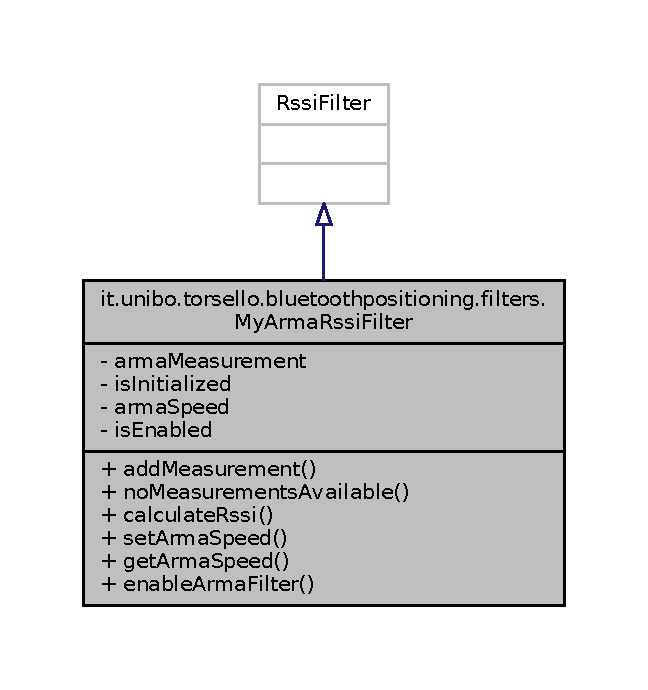
\includegraphics[width=311pt]{classit_1_1unibo_1_1torsello_1_1bluetoothpositioning_1_1filters_1_1MyArmaRssiFilter__inherit__graph}
\end{center}
\end{figure}


Diagramma di collaborazione per it.\+unibo.\+torsello.\+bluetoothpositioning.\+filters.\+My\+Arma\+Rssi\+Filter\+:
\nopagebreak
\begin{figure}[H]
\begin{center}
\leavevmode
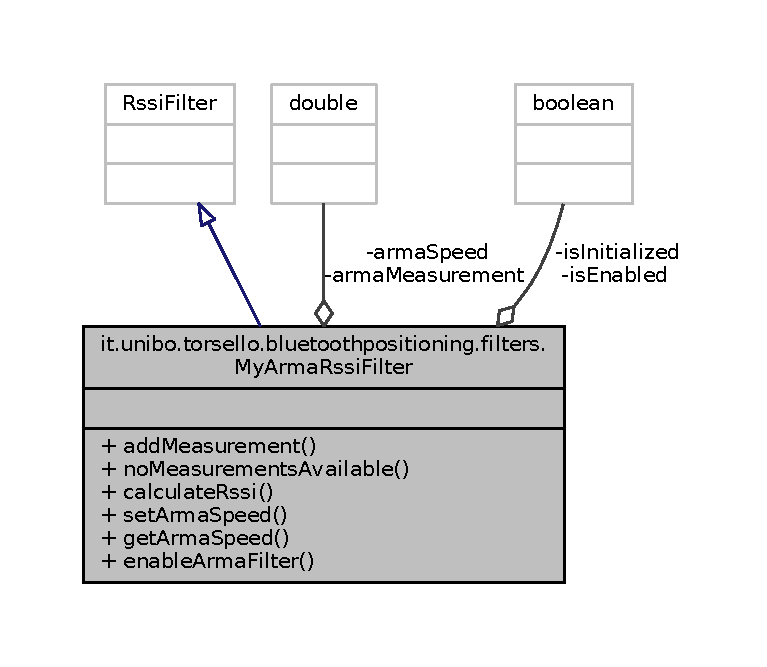
\includegraphics[width=350pt]{classit_1_1unibo_1_1torsello_1_1bluetoothpositioning_1_1filters_1_1MyArmaRssiFilter__coll__graph}
\end{center}
\end{figure}
\subsubsection*{Membri pubblici}
\begin{DoxyCompactItemize}
\item 
void \hyperlink{classit_1_1unibo_1_1torsello_1_1bluetoothpositioning_1_1filters_1_1MyArmaRssiFilter_afdb5386fe2b25ac048a992fb70de2f65_afdb5386fe2b25ac048a992fb70de2f65}{add\+Measurement} (Integer rssi)
\item 
boolean \hyperlink{classit_1_1unibo_1_1torsello_1_1bluetoothpositioning_1_1filters_1_1MyArmaRssiFilter_aa193a557e770f602ed998c4eacea2b41_aa193a557e770f602ed998c4eacea2b41}{no\+Measurements\+Available} ()
\item 
double \hyperlink{classit_1_1unibo_1_1torsello_1_1bluetoothpositioning_1_1filters_1_1MyArmaRssiFilter_a6414fddd8e0ae858df58b900a58bcc6f_a6414fddd8e0ae858df58b900a58bcc6f}{calculate\+Rssi} ()
\end{DoxyCompactItemize}
\subsubsection*{Membri pubblici statici}
\begin{DoxyCompactItemize}
\item 
static void \hyperlink{classit_1_1unibo_1_1torsello_1_1bluetoothpositioning_1_1filters_1_1MyArmaRssiFilter_aba1608e8dede3a85c42c084ac6326851_aba1608e8dede3a85c42c084ac6326851}{set\+Arma\+Speed} (double arma\+\_\+speed)
\item 
static double \hyperlink{classit_1_1unibo_1_1torsello_1_1bluetoothpositioning_1_1filters_1_1MyArmaRssiFilter_ac6eda6fc101dc89f3497c0ba8991658b_ac6eda6fc101dc89f3497c0ba8991658b}{get\+Arma\+Speed} ()
\item 
static void \hyperlink{classit_1_1unibo_1_1torsello_1_1bluetoothpositioning_1_1filters_1_1MyArmaRssiFilter_a36d7f50fdd722fe01bf86f21246d4151_a36d7f50fdd722fe01bf86f21246d4151}{enable\+Arma\+Filter} (boolean set)
\end{DoxyCompactItemize}
\subsubsection*{Attributi privati}
\begin{DoxyCompactItemize}
\item 
double \hyperlink{classit_1_1unibo_1_1torsello_1_1bluetoothpositioning_1_1filters_1_1MyArmaRssiFilter_ac386c808d409a1e6fc68801a3c2cf4b9_ac386c808d409a1e6fc68801a3c2cf4b9}{arma\+Measurement}
\item 
boolean \hyperlink{classit_1_1unibo_1_1torsello_1_1bluetoothpositioning_1_1filters_1_1MyArmaRssiFilter_a77ff83671b040ea636a1bb939803450b_a77ff83671b040ea636a1bb939803450b}{is\+Initialized} = false
\end{DoxyCompactItemize}
\subsubsection*{Attributi privati statici}
\begin{DoxyCompactItemize}
\item 
static double \hyperlink{classit_1_1unibo_1_1torsello_1_1bluetoothpositioning_1_1filters_1_1MyArmaRssiFilter_a55fe96a8f80f6ec634e4f9f9e2e337f8_a55fe96a8f80f6ec634e4f9f9e2e337f8}{arma\+Speed} = 0.\+1D
\item 
static boolean \hyperlink{classit_1_1unibo_1_1torsello_1_1bluetoothpositioning_1_1filters_1_1MyArmaRssiFilter_abff3147d8a5700ce103cd355d7b2b7d7_abff3147d8a5700ce103cd355d7b2b7d7}{is\+Enabled} = true
\end{DoxyCompactItemize}


\subsubsection{Descrizione dettagliata}
Created by Federico Torsello. \href{mailto:federico.torsello@studio.unibo.it}{\tt federico.\+torsello@studio.\+unibo.\+it} 

\subsubsection{Documentazione delle funzioni membro}
\hypertarget{classit_1_1unibo_1_1torsello_1_1bluetoothpositioning_1_1filters_1_1MyArmaRssiFilter_afdb5386fe2b25ac048a992fb70de2f65_afdb5386fe2b25ac048a992fb70de2f65}{}\label{classit_1_1unibo_1_1torsello_1_1bluetoothpositioning_1_1filters_1_1MyArmaRssiFilter_afdb5386fe2b25ac048a992fb70de2f65_afdb5386fe2b25ac048a992fb70de2f65} 
\index{it\+::unibo\+::torsello\+::bluetoothpositioning\+::filters\+::\+My\+Arma\+Rssi\+Filter@{it\+::unibo\+::torsello\+::bluetoothpositioning\+::filters\+::\+My\+Arma\+Rssi\+Filter}!add\+Measurement@{add\+Measurement}}
\index{add\+Measurement@{add\+Measurement}!it\+::unibo\+::torsello\+::bluetoothpositioning\+::filters\+::\+My\+Arma\+Rssi\+Filter@{it\+::unibo\+::torsello\+::bluetoothpositioning\+::filters\+::\+My\+Arma\+Rssi\+Filter}}
\paragraph{\texorpdfstring{add\+Measurement()}{addMeasurement()}}
{\footnotesize\ttfamily void it.\+unibo.\+torsello.\+bluetoothpositioning.\+filters.\+My\+Arma\+Rssi\+Filter.\+add\+Measurement (\begin{DoxyParamCaption}\item[{Integer}]{rssi }\end{DoxyParamCaption})}


\begin{DoxyCode}
30                                              \{
31 
32         \textcolor{keywordflow}{if} (\hyperlink{classit_1_1unibo_1_1torsello_1_1bluetoothpositioning_1_1filters_1_1MyArmaRssiFilter_abff3147d8a5700ce103cd355d7b2b7d7_abff3147d8a5700ce103cd355d7b2b7d7}{isEnabled}) \{
33             \textcolor{keywordflow}{if} (!\hyperlink{classit_1_1unibo_1_1torsello_1_1bluetoothpositioning_1_1filters_1_1MyArmaRssiFilter_a77ff83671b040ea636a1bb939803450b_a77ff83671b040ea636a1bb939803450b}{isInitialized}) \{
34                 \hyperlink{classit_1_1unibo_1_1torsello_1_1bluetoothpositioning_1_1filters_1_1MyArmaRssiFilter_ac386c808d409a1e6fc68801a3c2cf4b9_ac386c808d409a1e6fc68801a3c2cf4b9}{armaMeasurement} = rssi;
35                 \hyperlink{classit_1_1unibo_1_1torsello_1_1bluetoothpositioning_1_1filters_1_1MyArmaRssiFilter_a77ff83671b040ea636a1bb939803450b_a77ff83671b040ea636a1bb939803450b}{isInitialized} = \textcolor{keyword}{true};
36             \}
37 
38             \hyperlink{classit_1_1unibo_1_1torsello_1_1bluetoothpositioning_1_1filters_1_1MyArmaRssiFilter_ac386c808d409a1e6fc68801a3c2cf4b9_ac386c808d409a1e6fc68801a3c2cf4b9}{armaMeasurement} = (\hyperlink{classit_1_1unibo_1_1torsello_1_1bluetoothpositioning_1_1filters_1_1MyArmaRssiFilter_ac386c808d409a1e6fc68801a3c2cf4b9_ac386c808d409a1e6fc68801a3c2cf4b9}{armaMeasurement} - 
      \hyperlink{classit_1_1unibo_1_1torsello_1_1bluetoothpositioning_1_1filters_1_1MyArmaRssiFilter_a55fe96a8f80f6ec634e4f9f9e2e337f8_a55fe96a8f80f6ec634e4f9f9e2e337f8}{armaSpeed} * (\hyperlink{classit_1_1unibo_1_1torsello_1_1bluetoothpositioning_1_1filters_1_1MyArmaRssiFilter_ac386c808d409a1e6fc68801a3c2cf4b9_ac386c808d409a1e6fc68801a3c2cf4b9}{armaMeasurement} - rssi));
39         \} \textcolor{keywordflow}{else} \{
40             \hyperlink{classit_1_1unibo_1_1torsello_1_1bluetoothpositioning_1_1filters_1_1MyArmaRssiFilter_ac386c808d409a1e6fc68801a3c2cf4b9_ac386c808d409a1e6fc68801a3c2cf4b9}{armaMeasurement} = rssi;
41         \}
42 
43     \}
\end{DoxyCode}
\hypertarget{classit_1_1unibo_1_1torsello_1_1bluetoothpositioning_1_1filters_1_1MyArmaRssiFilter_a6414fddd8e0ae858df58b900a58bcc6f_a6414fddd8e0ae858df58b900a58bcc6f}{}\label{classit_1_1unibo_1_1torsello_1_1bluetoothpositioning_1_1filters_1_1MyArmaRssiFilter_a6414fddd8e0ae858df58b900a58bcc6f_a6414fddd8e0ae858df58b900a58bcc6f} 
\index{it\+::unibo\+::torsello\+::bluetoothpositioning\+::filters\+::\+My\+Arma\+Rssi\+Filter@{it\+::unibo\+::torsello\+::bluetoothpositioning\+::filters\+::\+My\+Arma\+Rssi\+Filter}!calculate\+Rssi@{calculate\+Rssi}}
\index{calculate\+Rssi@{calculate\+Rssi}!it\+::unibo\+::torsello\+::bluetoothpositioning\+::filters\+::\+My\+Arma\+Rssi\+Filter@{it\+::unibo\+::torsello\+::bluetoothpositioning\+::filters\+::\+My\+Arma\+Rssi\+Filter}}
\paragraph{\texorpdfstring{calculate\+Rssi()}{calculateRssi()}}
{\footnotesize\ttfamily double it.\+unibo.\+torsello.\+bluetoothpositioning.\+filters.\+My\+Arma\+Rssi\+Filter.\+calculate\+Rssi (\begin{DoxyParamCaption}{ }\end{DoxyParamCaption})}


\begin{DoxyCode}
51                                   \{
52         \textcolor{keywordflow}{return} \hyperlink{classit_1_1unibo_1_1torsello_1_1bluetoothpositioning_1_1filters_1_1MyArmaRssiFilter_ac386c808d409a1e6fc68801a3c2cf4b9_ac386c808d409a1e6fc68801a3c2cf4b9}{armaMeasurement};
53     \}
\end{DoxyCode}
\hypertarget{classit_1_1unibo_1_1torsello_1_1bluetoothpositioning_1_1filters_1_1MyArmaRssiFilter_a36d7f50fdd722fe01bf86f21246d4151_a36d7f50fdd722fe01bf86f21246d4151}{}\label{classit_1_1unibo_1_1torsello_1_1bluetoothpositioning_1_1filters_1_1MyArmaRssiFilter_a36d7f50fdd722fe01bf86f21246d4151_a36d7f50fdd722fe01bf86f21246d4151} 
\index{it\+::unibo\+::torsello\+::bluetoothpositioning\+::filters\+::\+My\+Arma\+Rssi\+Filter@{it\+::unibo\+::torsello\+::bluetoothpositioning\+::filters\+::\+My\+Arma\+Rssi\+Filter}!enable\+Arma\+Filter@{enable\+Arma\+Filter}}
\index{enable\+Arma\+Filter@{enable\+Arma\+Filter}!it\+::unibo\+::torsello\+::bluetoothpositioning\+::filters\+::\+My\+Arma\+Rssi\+Filter@{it\+::unibo\+::torsello\+::bluetoothpositioning\+::filters\+::\+My\+Arma\+Rssi\+Filter}}
\paragraph{\texorpdfstring{enable\+Arma\+Filter()}{enableArmaFilter()}}
{\footnotesize\ttfamily static void it.\+unibo.\+torsello.\+bluetoothpositioning.\+filters.\+My\+Arma\+Rssi\+Filter.\+enable\+Arma\+Filter (\begin{DoxyParamCaption}\item[{boolean}]{set }\end{DoxyParamCaption})\hspace{0.3cm}{\ttfamily [static]}}


\begin{DoxyCode}
25                                                      \{
26         \hyperlink{classit_1_1unibo_1_1torsello_1_1bluetoothpositioning_1_1filters_1_1MyArmaRssiFilter_abff3147d8a5700ce103cd355d7b2b7d7_abff3147d8a5700ce103cd355d7b2b7d7}{isEnabled} = \textcolor{keyword}{set};
27     \}
\end{DoxyCode}
\hypertarget{classit_1_1unibo_1_1torsello_1_1bluetoothpositioning_1_1filters_1_1MyArmaRssiFilter_ac6eda6fc101dc89f3497c0ba8991658b_ac6eda6fc101dc89f3497c0ba8991658b}{}\label{classit_1_1unibo_1_1torsello_1_1bluetoothpositioning_1_1filters_1_1MyArmaRssiFilter_ac6eda6fc101dc89f3497c0ba8991658b_ac6eda6fc101dc89f3497c0ba8991658b} 
\index{it\+::unibo\+::torsello\+::bluetoothpositioning\+::filters\+::\+My\+Arma\+Rssi\+Filter@{it\+::unibo\+::torsello\+::bluetoothpositioning\+::filters\+::\+My\+Arma\+Rssi\+Filter}!get\+Arma\+Speed@{get\+Arma\+Speed}}
\index{get\+Arma\+Speed@{get\+Arma\+Speed}!it\+::unibo\+::torsello\+::bluetoothpositioning\+::filters\+::\+My\+Arma\+Rssi\+Filter@{it\+::unibo\+::torsello\+::bluetoothpositioning\+::filters\+::\+My\+Arma\+Rssi\+Filter}}
\paragraph{\texorpdfstring{get\+Arma\+Speed()}{getArmaSpeed()}}
{\footnotesize\ttfamily static double it.\+unibo.\+torsello.\+bluetoothpositioning.\+filters.\+My\+Arma\+Rssi\+Filter.\+get\+Arma\+Speed (\begin{DoxyParamCaption}{ }\end{DoxyParamCaption})\hspace{0.3cm}{\ttfamily [static]}}


\begin{DoxyCode}
21                                         \{
22         \textcolor{keywordflow}{return} \hyperlink{classit_1_1unibo_1_1torsello_1_1bluetoothpositioning_1_1filters_1_1MyArmaRssiFilter_a55fe96a8f80f6ec634e4f9f9e2e337f8_a55fe96a8f80f6ec634e4f9f9e2e337f8}{armaSpeed};
23     \}
\end{DoxyCode}
\hypertarget{classit_1_1unibo_1_1torsello_1_1bluetoothpositioning_1_1filters_1_1MyArmaRssiFilter_aa193a557e770f602ed998c4eacea2b41_aa193a557e770f602ed998c4eacea2b41}{}\label{classit_1_1unibo_1_1torsello_1_1bluetoothpositioning_1_1filters_1_1MyArmaRssiFilter_aa193a557e770f602ed998c4eacea2b41_aa193a557e770f602ed998c4eacea2b41} 
\index{it\+::unibo\+::torsello\+::bluetoothpositioning\+::filters\+::\+My\+Arma\+Rssi\+Filter@{it\+::unibo\+::torsello\+::bluetoothpositioning\+::filters\+::\+My\+Arma\+Rssi\+Filter}!no\+Measurements\+Available@{no\+Measurements\+Available}}
\index{no\+Measurements\+Available@{no\+Measurements\+Available}!it\+::unibo\+::torsello\+::bluetoothpositioning\+::filters\+::\+My\+Arma\+Rssi\+Filter@{it\+::unibo\+::torsello\+::bluetoothpositioning\+::filters\+::\+My\+Arma\+Rssi\+Filter}}
\paragraph{\texorpdfstring{no\+Measurements\+Available()}{noMeasurementsAvailable()}}
{\footnotesize\ttfamily boolean it.\+unibo.\+torsello.\+bluetoothpositioning.\+filters.\+My\+Arma\+Rssi\+Filter.\+no\+Measurements\+Available (\begin{DoxyParamCaption}{ }\end{DoxyParamCaption})}


\begin{DoxyCode}
46                                              \{
47         \textcolor{keywordflow}{return} \textcolor{keyword}{false};
48     \}
\end{DoxyCode}
\hypertarget{classit_1_1unibo_1_1torsello_1_1bluetoothpositioning_1_1filters_1_1MyArmaRssiFilter_aba1608e8dede3a85c42c084ac6326851_aba1608e8dede3a85c42c084ac6326851}{}\label{classit_1_1unibo_1_1torsello_1_1bluetoothpositioning_1_1filters_1_1MyArmaRssiFilter_aba1608e8dede3a85c42c084ac6326851_aba1608e8dede3a85c42c084ac6326851} 
\index{it\+::unibo\+::torsello\+::bluetoothpositioning\+::filters\+::\+My\+Arma\+Rssi\+Filter@{it\+::unibo\+::torsello\+::bluetoothpositioning\+::filters\+::\+My\+Arma\+Rssi\+Filter}!set\+Arma\+Speed@{set\+Arma\+Speed}}
\index{set\+Arma\+Speed@{set\+Arma\+Speed}!it\+::unibo\+::torsello\+::bluetoothpositioning\+::filters\+::\+My\+Arma\+Rssi\+Filter@{it\+::unibo\+::torsello\+::bluetoothpositioning\+::filters\+::\+My\+Arma\+Rssi\+Filter}}
\paragraph{\texorpdfstring{set\+Arma\+Speed()}{setArmaSpeed()}}
{\footnotesize\ttfamily static void it.\+unibo.\+torsello.\+bluetoothpositioning.\+filters.\+My\+Arma\+Rssi\+Filter.\+set\+Arma\+Speed (\begin{DoxyParamCaption}\item[{double}]{arma\+\_\+speed }\end{DoxyParamCaption})\hspace{0.3cm}{\ttfamily [static]}}


\begin{DoxyCode}
17                                                        \{
18         \hyperlink{classit_1_1unibo_1_1torsello_1_1bluetoothpositioning_1_1filters_1_1MyArmaRssiFilter_a55fe96a8f80f6ec634e4f9f9e2e337f8_a55fe96a8f80f6ec634e4f9f9e2e337f8}{armaSpeed} = arma\_speed;
19     \}
\end{DoxyCode}


\subsubsection{Documentazione dei membri dato}
\hypertarget{classit_1_1unibo_1_1torsello_1_1bluetoothpositioning_1_1filters_1_1MyArmaRssiFilter_ac386c808d409a1e6fc68801a3c2cf4b9_ac386c808d409a1e6fc68801a3c2cf4b9}{}\label{classit_1_1unibo_1_1torsello_1_1bluetoothpositioning_1_1filters_1_1MyArmaRssiFilter_ac386c808d409a1e6fc68801a3c2cf4b9_ac386c808d409a1e6fc68801a3c2cf4b9} 
\index{it\+::unibo\+::torsello\+::bluetoothpositioning\+::filters\+::\+My\+Arma\+Rssi\+Filter@{it\+::unibo\+::torsello\+::bluetoothpositioning\+::filters\+::\+My\+Arma\+Rssi\+Filter}!arma\+Measurement@{arma\+Measurement}}
\index{arma\+Measurement@{arma\+Measurement}!it\+::unibo\+::torsello\+::bluetoothpositioning\+::filters\+::\+My\+Arma\+Rssi\+Filter@{it\+::unibo\+::torsello\+::bluetoothpositioning\+::filters\+::\+My\+Arma\+Rssi\+Filter}}
\paragraph{\texorpdfstring{arma\+Measurement}{armaMeasurement}}
{\footnotesize\ttfamily double it.\+unibo.\+torsello.\+bluetoothpositioning.\+filters.\+My\+Arma\+Rssi\+Filter.\+arma\+Measurement\hspace{0.3cm}{\ttfamily [private]}}

\hypertarget{classit_1_1unibo_1_1torsello_1_1bluetoothpositioning_1_1filters_1_1MyArmaRssiFilter_a55fe96a8f80f6ec634e4f9f9e2e337f8_a55fe96a8f80f6ec634e4f9f9e2e337f8}{}\label{classit_1_1unibo_1_1torsello_1_1bluetoothpositioning_1_1filters_1_1MyArmaRssiFilter_a55fe96a8f80f6ec634e4f9f9e2e337f8_a55fe96a8f80f6ec634e4f9f9e2e337f8} 
\index{it\+::unibo\+::torsello\+::bluetoothpositioning\+::filters\+::\+My\+Arma\+Rssi\+Filter@{it\+::unibo\+::torsello\+::bluetoothpositioning\+::filters\+::\+My\+Arma\+Rssi\+Filter}!arma\+Speed@{arma\+Speed}}
\index{arma\+Speed@{arma\+Speed}!it\+::unibo\+::torsello\+::bluetoothpositioning\+::filters\+::\+My\+Arma\+Rssi\+Filter@{it\+::unibo\+::torsello\+::bluetoothpositioning\+::filters\+::\+My\+Arma\+Rssi\+Filter}}
\paragraph{\texorpdfstring{arma\+Speed}{armaSpeed}}
{\footnotesize\ttfamily double it.\+unibo.\+torsello.\+bluetoothpositioning.\+filters.\+My\+Arma\+Rssi\+Filter.\+arma\+Speed = 0.\+1D\hspace{0.3cm}{\ttfamily [static]}, {\ttfamily [private]}}

\hypertarget{classit_1_1unibo_1_1torsello_1_1bluetoothpositioning_1_1filters_1_1MyArmaRssiFilter_abff3147d8a5700ce103cd355d7b2b7d7_abff3147d8a5700ce103cd355d7b2b7d7}{}\label{classit_1_1unibo_1_1torsello_1_1bluetoothpositioning_1_1filters_1_1MyArmaRssiFilter_abff3147d8a5700ce103cd355d7b2b7d7_abff3147d8a5700ce103cd355d7b2b7d7} 
\index{it\+::unibo\+::torsello\+::bluetoothpositioning\+::filters\+::\+My\+Arma\+Rssi\+Filter@{it\+::unibo\+::torsello\+::bluetoothpositioning\+::filters\+::\+My\+Arma\+Rssi\+Filter}!is\+Enabled@{is\+Enabled}}
\index{is\+Enabled@{is\+Enabled}!it\+::unibo\+::torsello\+::bluetoothpositioning\+::filters\+::\+My\+Arma\+Rssi\+Filter@{it\+::unibo\+::torsello\+::bluetoothpositioning\+::filters\+::\+My\+Arma\+Rssi\+Filter}}
\paragraph{\texorpdfstring{is\+Enabled}{isEnabled}}
{\footnotesize\ttfamily boolean it.\+unibo.\+torsello.\+bluetoothpositioning.\+filters.\+My\+Arma\+Rssi\+Filter.\+is\+Enabled = true\hspace{0.3cm}{\ttfamily [static]}, {\ttfamily [private]}}

\hypertarget{classit_1_1unibo_1_1torsello_1_1bluetoothpositioning_1_1filters_1_1MyArmaRssiFilter_a77ff83671b040ea636a1bb939803450b_a77ff83671b040ea636a1bb939803450b}{}\label{classit_1_1unibo_1_1torsello_1_1bluetoothpositioning_1_1filters_1_1MyArmaRssiFilter_a77ff83671b040ea636a1bb939803450b_a77ff83671b040ea636a1bb939803450b} 
\index{it\+::unibo\+::torsello\+::bluetoothpositioning\+::filters\+::\+My\+Arma\+Rssi\+Filter@{it\+::unibo\+::torsello\+::bluetoothpositioning\+::filters\+::\+My\+Arma\+Rssi\+Filter}!is\+Initialized@{is\+Initialized}}
\index{is\+Initialized@{is\+Initialized}!it\+::unibo\+::torsello\+::bluetoothpositioning\+::filters\+::\+My\+Arma\+Rssi\+Filter@{it\+::unibo\+::torsello\+::bluetoothpositioning\+::filters\+::\+My\+Arma\+Rssi\+Filter}}
\paragraph{\texorpdfstring{is\+Initialized}{isInitialized}}
{\footnotesize\ttfamily boolean it.\+unibo.\+torsello.\+bluetoothpositioning.\+filters.\+My\+Arma\+Rssi\+Filter.\+is\+Initialized = false\hspace{0.3cm}{\ttfamily [private]}}



La documentazione per questa classe è stata generata a partire dal seguente file\+:\begin{DoxyCompactItemize}
\item 
\hyperlink{MyArmaRssiFilter_8java}{My\+Arma\+Rssi\+Filter.\+java}\end{DoxyCompactItemize}

\hypertarget{interfaceit_1_1unibo_1_1torsello_1_1bluetoothpositioning_1_1fragment_1_1DeviceDetailInner0Fragment_1_1OnRecordingReport}{}\subsection{Riferimenti per l\textquotesingle{}interfaccia it.\+unibo.\+torsello.\+bluetoothpositioning.\+fragment.\+Device\+Detail\+Inner0\+Fragment.\+On\+Recording\+Report}
\label{interfaceit_1_1unibo_1_1torsello_1_1bluetoothpositioning_1_1fragment_1_1DeviceDetailInner0Fragment_1_1OnRecordingReport}\index{it.\+unibo.\+torsello.\+bluetoothpositioning.\+fragment.\+Device\+Detail\+Inner0\+Fragment.\+On\+Recording\+Report@{it.\+unibo.\+torsello.\+bluetoothpositioning.\+fragment.\+Device\+Detail\+Inner0\+Fragment.\+On\+Recording\+Report}}


Diagramma delle classi per it.\+unibo.\+torsello.\+bluetoothpositioning.\+fragment.\+Device\+Detail\+Inner0\+Fragment.\+On\+Recording\+Report
\nopagebreak
\begin{figure}[H]
\begin{center}
\leavevmode
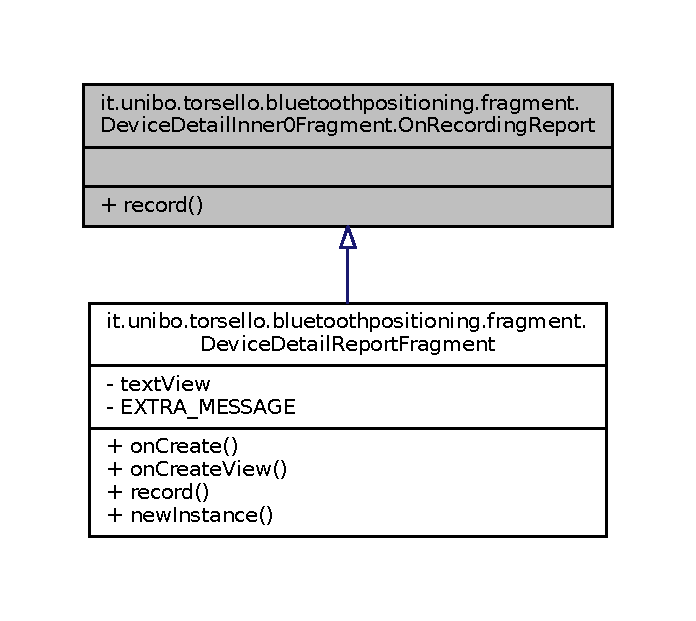
\includegraphics[width=334pt]{interfaceit_1_1unibo_1_1torsello_1_1bluetoothpositioning_1_1fragment_1_1DeviceDetailInner0Fragme771da81ee79947fcb94bf26bc1164f62}
\end{center}
\end{figure}


Diagramma di collaborazione per it.\+unibo.\+torsello.\+bluetoothpositioning.\+fragment.\+Device\+Detail\+Inner0\+Fragment.\+On\+Recording\+Report\+:
\nopagebreak
\begin{figure}[H]
\begin{center}
\leavevmode
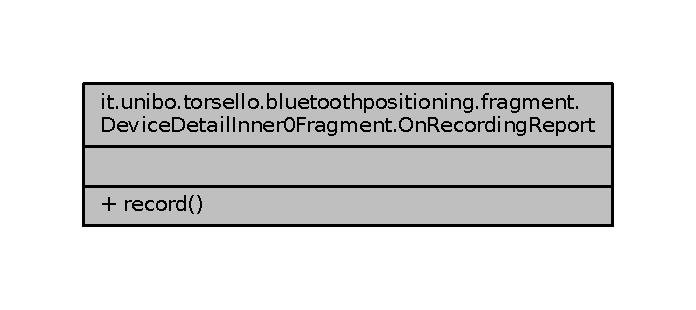
\includegraphics[width=334pt]{interfaceit_1_1unibo_1_1torsello_1_1bluetoothpositioning_1_1fragment_1_1DeviceDetailInner0Fragme10bd69251886d8905e7bf739086755ab}
\end{center}
\end{figure}
\subsubsection*{Membri pubblici}
\begin{DoxyCompactItemize}
\item 
void \hyperlink{interfaceit_1_1unibo_1_1torsello_1_1bluetoothpositioning_1_1fragment_1_1DeviceDetailInner0Fragment_1_1OnRecordingReport_a63fd189046ae9d716c19b152957f6c74_a63fd189046ae9d716c19b152957f6c74}{record} (String new\+Record)
\end{DoxyCompactItemize}


\subsubsection{Documentazione delle funzioni membro}
\hypertarget{interfaceit_1_1unibo_1_1torsello_1_1bluetoothpositioning_1_1fragment_1_1DeviceDetailInner0Fragment_1_1OnRecordingReport_a63fd189046ae9d716c19b152957f6c74_a63fd189046ae9d716c19b152957f6c74}{}\label{interfaceit_1_1unibo_1_1torsello_1_1bluetoothpositioning_1_1fragment_1_1DeviceDetailInner0Fragment_1_1OnRecordingReport_a63fd189046ae9d716c19b152957f6c74_a63fd189046ae9d716c19b152957f6c74} 
\index{it\+::unibo\+::torsello\+::bluetoothpositioning\+::fragment\+::\+Device\+Detail\+Inner0\+Fragment\+::\+On\+Recording\+Report@{it\+::unibo\+::torsello\+::bluetoothpositioning\+::fragment\+::\+Device\+Detail\+Inner0\+Fragment\+::\+On\+Recording\+Report}!record@{record}}
\index{record@{record}!it\+::unibo\+::torsello\+::bluetoothpositioning\+::fragment\+::\+Device\+Detail\+Inner0\+Fragment\+::\+On\+Recording\+Report@{it\+::unibo\+::torsello\+::bluetoothpositioning\+::fragment\+::\+Device\+Detail\+Inner0\+Fragment\+::\+On\+Recording\+Report}}
\paragraph{\texorpdfstring{record()}{record()}}
{\footnotesize\ttfamily void it.\+unibo.\+torsello.\+bluetoothpositioning.\+fragment.\+Device\+Detail\+Inner0\+Fragment.\+On\+Recording\+Report.\+record (\begin{DoxyParamCaption}\item[{String}]{new\+Record }\end{DoxyParamCaption})}



Implementato in \hyperlink{classit_1_1unibo_1_1torsello_1_1bluetoothpositioning_1_1fragment_1_1DeviceDetailReportFragment_ae9615d2a2096700befd416d0d8a95f85_ae9615d2a2096700befd416d0d8a95f85}{it.\+unibo.\+torsello.\+bluetoothpositioning.\+fragment.\+Device\+Detail\+Report\+Fragment}.



La documentazione per questa interfaccia è stata generata a partire dal seguente file\+:\begin{DoxyCompactItemize}
\item 
\hyperlink{DeviceDetailInner0Fragment_8java}{Device\+Detail\+Inner0\+Fragment.\+java}\end{DoxyCompactItemize}

\hypertarget{interfaceit_1_1unibo_1_1torsello_1_1bluetoothpositioning_1_1fragment_1_1DeviceDetailInner0Fragment_1_1OnRecordingResume}{}\subsection{Riferimenti per l\textquotesingle{}interfaccia it.\+unibo.\+torsello.\+bluetoothpositioning.\+fragment.\+Device\+Detail\+Inner0\+Fragment.\+On\+Recording\+Resume}
\label{interfaceit_1_1unibo_1_1torsello_1_1bluetoothpositioning_1_1fragment_1_1DeviceDetailInner0Fragment_1_1OnRecordingResume}\index{it.\+unibo.\+torsello.\+bluetoothpositioning.\+fragment.\+Device\+Detail\+Inner0\+Fragment.\+On\+Recording\+Resume@{it.\+unibo.\+torsello.\+bluetoothpositioning.\+fragment.\+Device\+Detail\+Inner0\+Fragment.\+On\+Recording\+Resume}}


Diagramma delle classi per it.\+unibo.\+torsello.\+bluetoothpositioning.\+fragment.\+Device\+Detail\+Inner0\+Fragment.\+On\+Recording\+Resume
\nopagebreak
\begin{figure}[H]
\begin{center}
\leavevmode
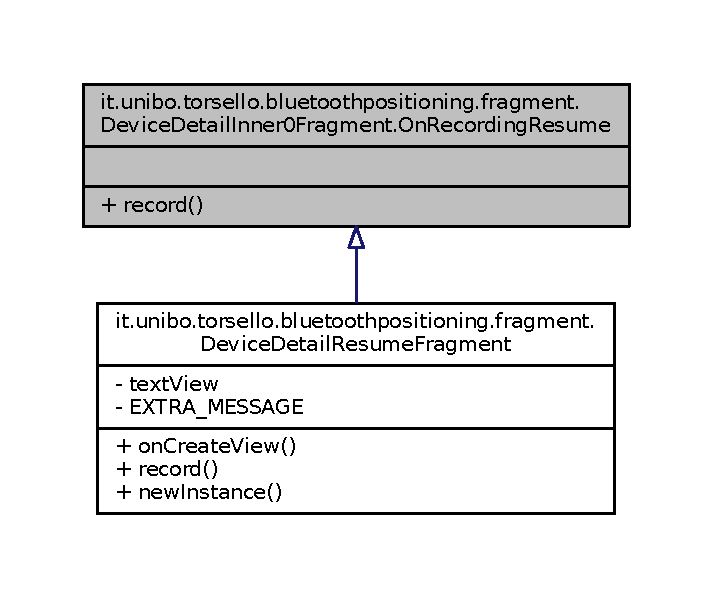
\includegraphics[width=342pt]{interfaceit_1_1unibo_1_1torsello_1_1bluetoothpositioning_1_1fragment_1_1DeviceDetailInner0Fragme43535f1396450c17cd5f3da229ebde14}
\end{center}
\end{figure}


Diagramma di collaborazione per it.\+unibo.\+torsello.\+bluetoothpositioning.\+fragment.\+Device\+Detail\+Inner0\+Fragment.\+On\+Recording\+Resume\+:
\nopagebreak
\begin{figure}[H]
\begin{center}
\leavevmode
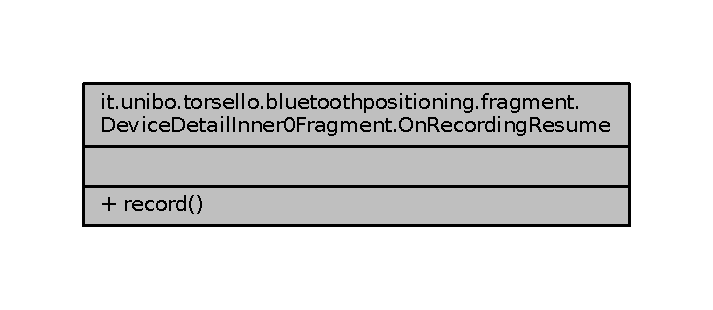
\includegraphics[width=342pt]{interfaceit_1_1unibo_1_1torsello_1_1bluetoothpositioning_1_1fragment_1_1DeviceDetailInner0Fragmec6511fc8aea77ecfd2776fc4eae14545}
\end{center}
\end{figure}
\subsubsection*{Membri pubblici}
\begin{DoxyCompactItemize}
\item 
void \hyperlink{interfaceit_1_1unibo_1_1torsello_1_1bluetoothpositioning_1_1fragment_1_1DeviceDetailInner0Fragment_1_1OnRecordingResume_a68528e5fbaa02cb01776eba68da833d8_a68528e5fbaa02cb01776eba68da833d8}{record} (String new\+Record)
\end{DoxyCompactItemize}


\subsubsection{Documentazione delle funzioni membro}
\hypertarget{interfaceit_1_1unibo_1_1torsello_1_1bluetoothpositioning_1_1fragment_1_1DeviceDetailInner0Fragment_1_1OnRecordingResume_a68528e5fbaa02cb01776eba68da833d8_a68528e5fbaa02cb01776eba68da833d8}{}\label{interfaceit_1_1unibo_1_1torsello_1_1bluetoothpositioning_1_1fragment_1_1DeviceDetailInner0Fragment_1_1OnRecordingResume_a68528e5fbaa02cb01776eba68da833d8_a68528e5fbaa02cb01776eba68da833d8} 
\index{it\+::unibo\+::torsello\+::bluetoothpositioning\+::fragment\+::\+Device\+Detail\+Inner0\+Fragment\+::\+On\+Recording\+Resume@{it\+::unibo\+::torsello\+::bluetoothpositioning\+::fragment\+::\+Device\+Detail\+Inner0\+Fragment\+::\+On\+Recording\+Resume}!record@{record}}
\index{record@{record}!it\+::unibo\+::torsello\+::bluetoothpositioning\+::fragment\+::\+Device\+Detail\+Inner0\+Fragment\+::\+On\+Recording\+Resume@{it\+::unibo\+::torsello\+::bluetoothpositioning\+::fragment\+::\+Device\+Detail\+Inner0\+Fragment\+::\+On\+Recording\+Resume}}
\paragraph{\texorpdfstring{record()}{record()}}
{\footnotesize\ttfamily void it.\+unibo.\+torsello.\+bluetoothpositioning.\+fragment.\+Device\+Detail\+Inner0\+Fragment.\+On\+Recording\+Resume.\+record (\begin{DoxyParamCaption}\item[{String}]{new\+Record }\end{DoxyParamCaption})}



Implementato in \hyperlink{classit_1_1unibo_1_1torsello_1_1bluetoothpositioning_1_1fragment_1_1DeviceDetailResumeFragment_aa4b3952d75b693caa46309f0f2ca05b4_aa4b3952d75b693caa46309f0f2ca05b4}{it.\+unibo.\+torsello.\+bluetoothpositioning.\+fragment.\+Device\+Detail\+Resume\+Fragment}.



La documentazione per questa interfaccia è stata generata a partire dal seguente file\+:\begin{DoxyCompactItemize}
\item 
\hyperlink{DeviceDetailInner0Fragment_8java}{Device\+Detail\+Inner0\+Fragment.\+java}\end{DoxyCompactItemize}

\hypertarget{classit_1_1unibo_1_1torsello_1_1bluetoothpositioning_1_1util_1_1ReportUtils}{}\subsection{Riferimenti per la classe it.\+unibo.\+torsello.\+bluetoothpositioning.\+util.\+Report\+Utils}
\label{classit_1_1unibo_1_1torsello_1_1bluetoothpositioning_1_1util_1_1ReportUtils}\index{it.\+unibo.\+torsello.\+bluetoothpositioning.\+util.\+Report\+Utils@{it.\+unibo.\+torsello.\+bluetoothpositioning.\+util.\+Report\+Utils}}


Diagramma di collaborazione per it.\+unibo.\+torsello.\+bluetoothpositioning.\+util.\+Report\+Utils\+:
\nopagebreak
\begin{figure}[H]
\begin{center}
\leavevmode
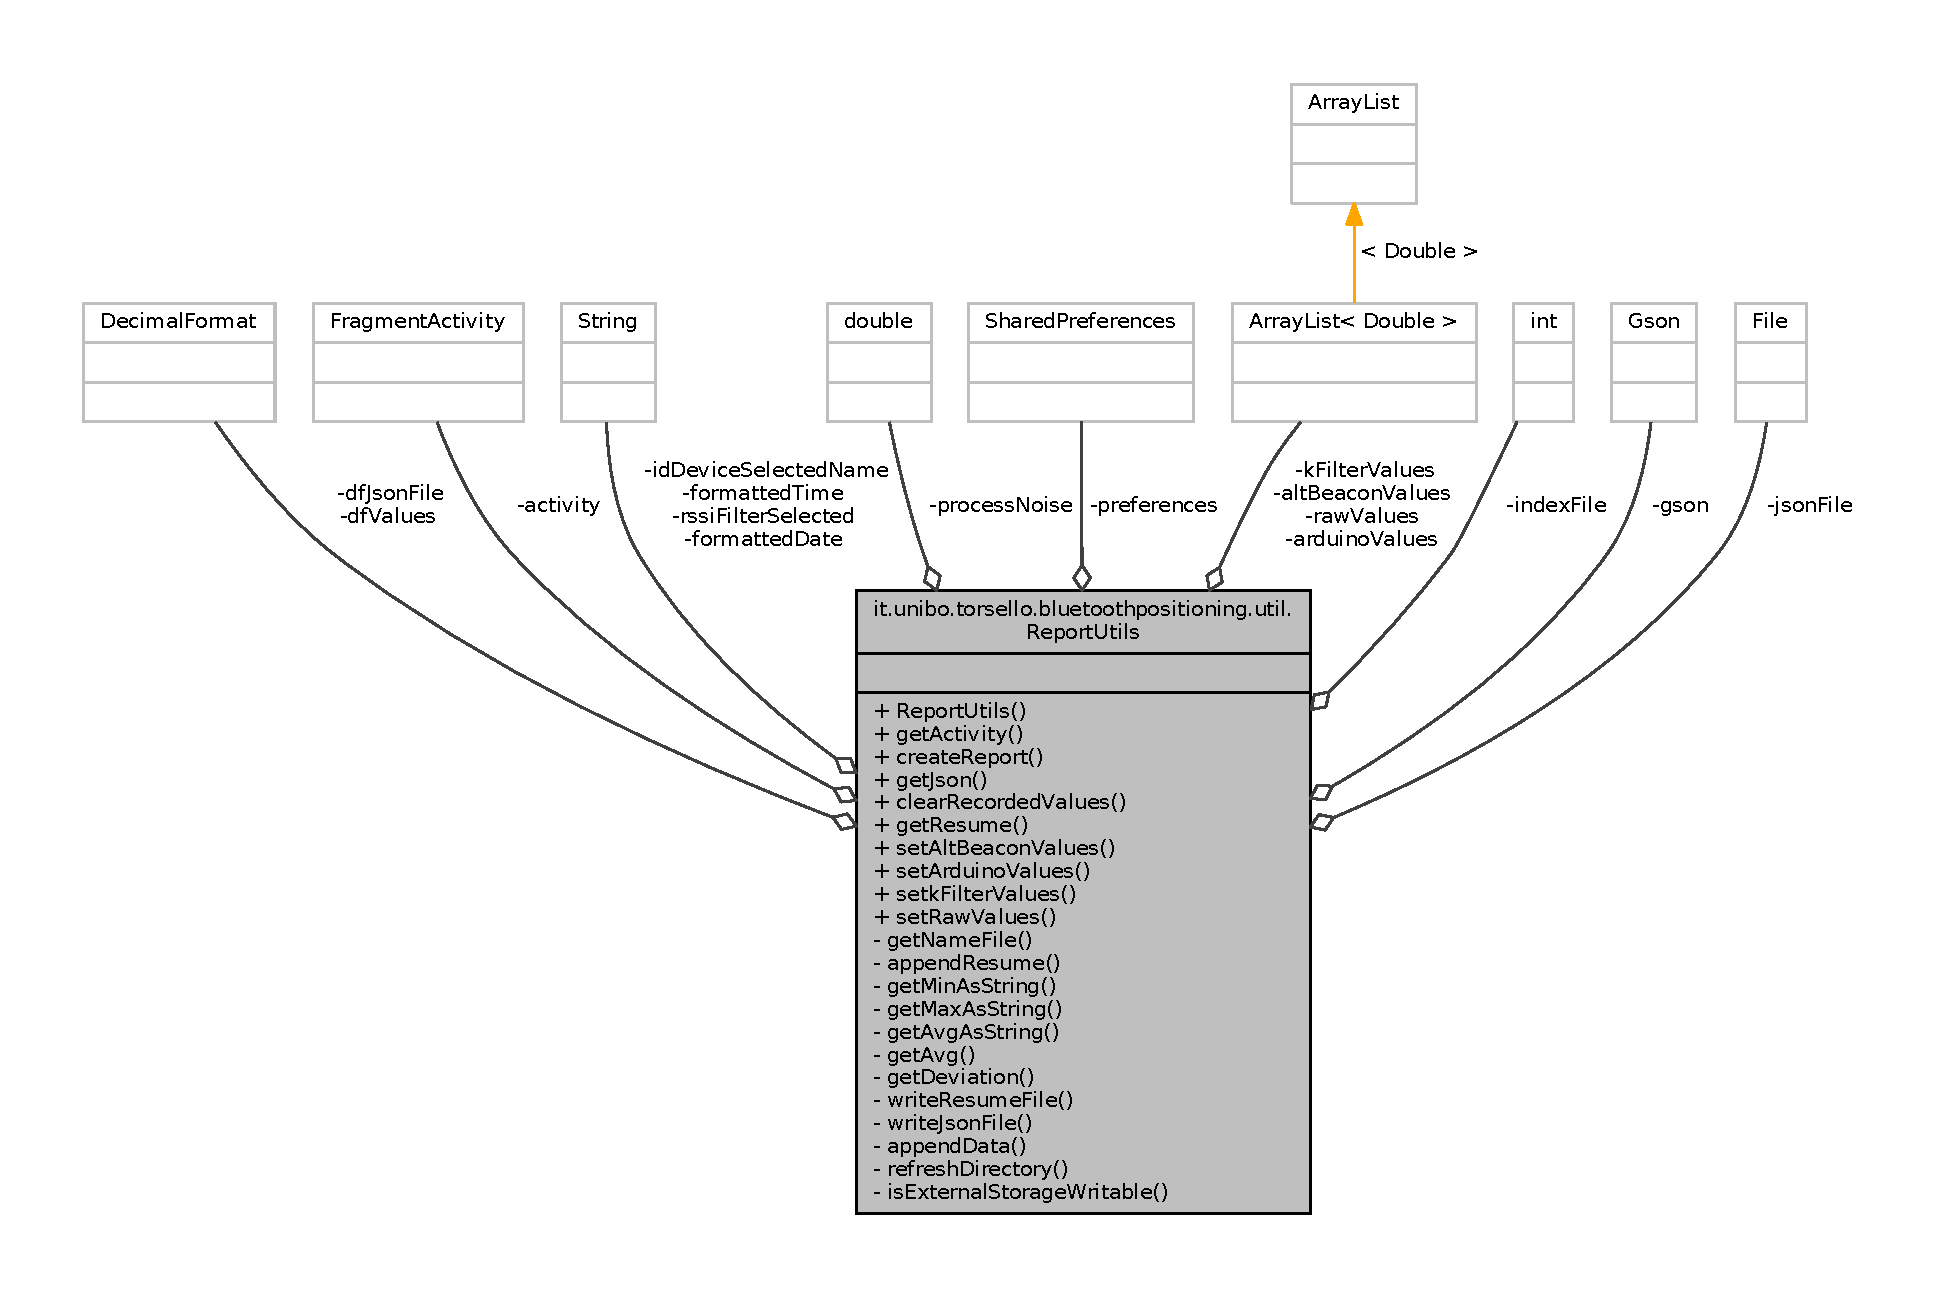
\includegraphics[width=350pt]{classit_1_1unibo_1_1torsello_1_1bluetoothpositioning_1_1util_1_1ReportUtils__coll__graph}
\end{center}
\end{figure}
\subsubsection*{Membri pubblici}
\begin{DoxyCompactItemize}
\item 
\hyperlink{classit_1_1unibo_1_1torsello_1_1bluetoothpositioning_1_1util_1_1ReportUtils_af9975aaf0a16c6a51afd258b8c3f77c0_af9975aaf0a16c6a51afd258b8c3f77c0}{Report\+Utils} (Fragment\+Activity fragment\+Activity, String device\+Name)
\item 
Fragment\+Activity \hyperlink{classit_1_1unibo_1_1torsello_1_1bluetoothpositioning_1_1util_1_1ReportUtils_a397da2904c606315301d19eb39451181_a397da2904c606315301d19eb39451181}{get\+Activity} ()
\item 
void \hyperlink{classit_1_1unibo_1_1torsello_1_1bluetoothpositioning_1_1util_1_1ReportUtils_a346661fa52c458c399de10f6ca494cd7_a346661fa52c458c399de10f6ca494cd7}{create\+Report} ()
\item 
String \hyperlink{classit_1_1unibo_1_1torsello_1_1bluetoothpositioning_1_1util_1_1ReportUtils_a768356af2517bb604a39daf2497fc761_a768356af2517bb604a39daf2497fc761}{get\+Json} ()
\item 
void \hyperlink{classit_1_1unibo_1_1torsello_1_1bluetoothpositioning_1_1util_1_1ReportUtils_aa83960dff58c2975a142c6b093abf72a_aa83960dff58c2975a142c6b093abf72a}{clear\+Recorded\+Values} ()
\item 
String \hyperlink{classit_1_1unibo_1_1torsello_1_1bluetoothpositioning_1_1util_1_1ReportUtils_a2b62843f2c0da4743686ca60edfc3aed_a2b62843f2c0da4743686ca60edfc3aed}{get\+Resume} ()
\item 
void \hyperlink{classit_1_1unibo_1_1torsello_1_1bluetoothpositioning_1_1util_1_1ReportUtils_ae68aaee9a1033dd6659cc3d6af970f60_ae68aaee9a1033dd6659cc3d6af970f60}{set\+Alt\+Beacon\+Values} (Double \hyperlink{classit_1_1unibo_1_1torsello_1_1bluetoothpositioning_1_1util_1_1ReportUtils_a6e72cc0d840390d44e6cbccece68e240_a6e72cc0d840390d44e6cbccece68e240}{alt\+Beacon\+Values})
\item 
void \hyperlink{classit_1_1unibo_1_1torsello_1_1bluetoothpositioning_1_1util_1_1ReportUtils_a3fbc76f4a952ebae654b238dbef6ca1d_a3fbc76f4a952ebae654b238dbef6ca1d}{set\+Arduino\+Values} (Double \hyperlink{classit_1_1unibo_1_1torsello_1_1bluetoothpositioning_1_1util_1_1ReportUtils_a3557dcc1662461b46fcd4d18eee9780e_a3557dcc1662461b46fcd4d18eee9780e}{arduino\+Values})
\item 
void \hyperlink{classit_1_1unibo_1_1torsello_1_1bluetoothpositioning_1_1util_1_1ReportUtils_a081697bebaa8ef8f7d245f9a7da917fa_a081697bebaa8ef8f7d245f9a7da917fa}{setk\+Filter\+Values} (Double \hyperlink{classit_1_1unibo_1_1torsello_1_1bluetoothpositioning_1_1util_1_1ReportUtils_a9a40344497c5522bbc90f03581c2713a_a9a40344497c5522bbc90f03581c2713a}{k\+Filter\+Values})
\item 
void \hyperlink{classit_1_1unibo_1_1torsello_1_1bluetoothpositioning_1_1util_1_1ReportUtils_a6a65fe55f37edba3871801600cdf48f4_a6a65fe55f37edba3871801600cdf48f4}{set\+Raw\+Values} (Double \hyperlink{classit_1_1unibo_1_1torsello_1_1bluetoothpositioning_1_1util_1_1ReportUtils_adbe56bea0813a48932ef94b8b27c3314_adbe56bea0813a48932ef94b8b27c3314}{raw\+Values})
\end{DoxyCompactItemize}
\subsubsection*{Membri privati}
\begin{DoxyCompactItemize}
\item 
String \hyperlink{classit_1_1unibo_1_1torsello_1_1bluetoothpositioning_1_1util_1_1ReportUtils_a0f5823e8ff4bd5e3accc20a7313b075f_a0f5823e8ff4bd5e3accc20a7313b075f}{get\+Name\+File} ()
\item 
String \hyperlink{classit_1_1unibo_1_1torsello_1_1bluetoothpositioning_1_1util_1_1ReportUtils_ac57226bb543cd32d89c205a41ff23ae3_ac57226bb543cd32d89c205a41ff23ae3}{append\+Resume} (String arg, Array\+List$<$ Double $>$ value)
\item 
String \hyperlink{classit_1_1unibo_1_1torsello_1_1bluetoothpositioning_1_1util_1_1ReportUtils_ad44a97d58ebf0e48fc15b573be05eae9_ad44a97d58ebf0e48fc15b573be05eae9}{get\+Min\+As\+String} (Array\+List$<$ Double $>$ value)
\item 
String \hyperlink{classit_1_1unibo_1_1torsello_1_1bluetoothpositioning_1_1util_1_1ReportUtils_ada05f889f861205ac0687db4442cad63_ada05f889f861205ac0687db4442cad63}{get\+Max\+As\+String} (Array\+List$<$ Double $>$ value)
\item 
String \hyperlink{classit_1_1unibo_1_1torsello_1_1bluetoothpositioning_1_1util_1_1ReportUtils_a174ea1d2c8b7e5effd484c65d1b5488c_a174ea1d2c8b7e5effd484c65d1b5488c}{get\+Avg\+As\+String} (Array\+List$<$ Double $>$ value)
\item 
Double \hyperlink{classit_1_1unibo_1_1torsello_1_1bluetoothpositioning_1_1util_1_1ReportUtils_a4efc733750ef3ab7dddb613291bff1c4_a4efc733750ef3ab7dddb613291bff1c4}{get\+Avg} (Array\+List$<$ Double $>$ value)
\item 
String \hyperlink{classit_1_1unibo_1_1torsello_1_1bluetoothpositioning_1_1util_1_1ReportUtils_af24755a01c03201bca86e0c2e03cf81d_af24755a01c03201bca86e0c2e03cf81d}{get\+Deviation} (Double value)
\item 
void \hyperlink{classit_1_1unibo_1_1torsello_1_1bluetoothpositioning_1_1util_1_1ReportUtils_af8578f11822b403410e46f023b68dd7b_af8578f11822b403410e46f023b68dd7b}{write\+Resume\+File} ()
\item 
void \hyperlink{classit_1_1unibo_1_1torsello_1_1bluetoothpositioning_1_1util_1_1ReportUtils_aa14b78ad82095e13e057308f4b5da594_aa14b78ad82095e13e057308f4b5da594}{write\+Json\+File} ()
\item 
Json\+Writer \hyperlink{classit_1_1unibo_1_1torsello_1_1bluetoothpositioning_1_1util_1_1ReportUtils_ad5cf6eb0aa41a0e3eeaabfec16f47c28_ad5cf6eb0aa41a0e3eeaabfec16f47c28}{append\+Data} (Json\+Writer jw, Array\+List$<$ Double $>$ value)  throws I\+O\+Exception 
\item 
void \hyperlink{classit_1_1unibo_1_1torsello_1_1bluetoothpositioning_1_1util_1_1ReportUtils_a5d2a51b68c3344f5aa41abaa118282b4_a5d2a51b68c3344f5aa41abaa118282b4}{refresh\+Directory} (File file)
\item 
boolean \hyperlink{classit_1_1unibo_1_1torsello_1_1bluetoothpositioning_1_1util_1_1ReportUtils_a58e7513f3cbe12723359b8dee541ed14_a58e7513f3cbe12723359b8dee541ed14}{is\+External\+Storage\+Writable} ()
\end{DoxyCompactItemize}
\subsubsection*{Attributi privati}
\begin{DoxyCompactItemize}
\item 
String \hyperlink{classit_1_1unibo_1_1torsello_1_1bluetoothpositioning_1_1util_1_1ReportUtils_a4c838a130a922b6f26b79c7d7bdcaf9c_a4c838a130a922b6f26b79c7d7bdcaf9c}{id\+Device\+Selected\+Name}
\item 
Fragment\+Activity \hyperlink{classit_1_1unibo_1_1torsello_1_1bluetoothpositioning_1_1util_1_1ReportUtils_ae36eb3321f2d7f96753d7854f5cb6923_ae36eb3321f2d7f96753d7854f5cb6923}{activity}
\item 
String \hyperlink{classit_1_1unibo_1_1torsello_1_1bluetoothpositioning_1_1util_1_1ReportUtils_ad51884bc9ff99e0ed1e7d5f8054de6da_ad51884bc9ff99e0ed1e7d5f8054de6da}{rssi\+Filter\+Selected}
\item 
Array\+List$<$ Double $>$ \hyperlink{classit_1_1unibo_1_1torsello_1_1bluetoothpositioning_1_1util_1_1ReportUtils_a3557dcc1662461b46fcd4d18eee9780e_a3557dcc1662461b46fcd4d18eee9780e}{arduino\+Values}
\item 
Array\+List$<$ Double $>$ \hyperlink{classit_1_1unibo_1_1torsello_1_1bluetoothpositioning_1_1util_1_1ReportUtils_adbe56bea0813a48932ef94b8b27c3314_adbe56bea0813a48932ef94b8b27c3314}{raw\+Values}
\item 
Array\+List$<$ Double $>$ \hyperlink{classit_1_1unibo_1_1torsello_1_1bluetoothpositioning_1_1util_1_1ReportUtils_a6e72cc0d840390d44e6cbccece68e240_a6e72cc0d840390d44e6cbccece68e240}{alt\+Beacon\+Values}
\item 
Array\+List$<$ Double $>$ \hyperlink{classit_1_1unibo_1_1torsello_1_1bluetoothpositioning_1_1util_1_1ReportUtils_a9a40344497c5522bbc90f03581c2713a_a9a40344497c5522bbc90f03581c2713a}{k\+Filter\+Values}
\item 
String \hyperlink{classit_1_1unibo_1_1torsello_1_1bluetoothpositioning_1_1util_1_1ReportUtils_a0339d8306f408d438720a67d1801f46c_a0339d8306f408d438720a67d1801f46c}{formatted\+Date}
\item 
String \hyperlink{classit_1_1unibo_1_1torsello_1_1bluetoothpositioning_1_1util_1_1ReportUtils_a6e6b0d302bb7d2e8f128154f0a80965c_a6e6b0d302bb7d2e8f128154f0a80965c}{formatted\+Time}
\item 
Decimal\+Format \hyperlink{classit_1_1unibo_1_1torsello_1_1bluetoothpositioning_1_1util_1_1ReportUtils_afb07df801c89068760b260fb09916895_afb07df801c89068760b260fb09916895}{df\+Values}
\item 
Decimal\+Format \hyperlink{classit_1_1unibo_1_1torsello_1_1bluetoothpositioning_1_1util_1_1ReportUtils_a29b88de66ca4b3e85b3cc86e9621c26a_a29b88de66ca4b3e85b3cc86e9621c26a}{df\+Json\+File}
\item 
Gson \hyperlink{classit_1_1unibo_1_1torsello_1_1bluetoothpositioning_1_1util_1_1ReportUtils_a974d9bac8edb83847a34b20db0299fca_a974d9bac8edb83847a34b20db0299fca}{gson}
\item 
File \hyperlink{classit_1_1unibo_1_1torsello_1_1bluetoothpositioning_1_1util_1_1ReportUtils_a3d54acab8d9785425b61d7a294444f85_a3d54acab8d9785425b61d7a294444f85}{json\+File}
\item 
int \hyperlink{classit_1_1unibo_1_1torsello_1_1bluetoothpositioning_1_1util_1_1ReportUtils_afcda83ce8a192e352a399e5454fcbba6_afcda83ce8a192e352a399e5454fcbba6}{index\+File} = 1
\item 
Shared\+Preferences \hyperlink{classit_1_1unibo_1_1torsello_1_1bluetoothpositioning_1_1util_1_1ReportUtils_af1f57227f8c42073b4f8f2b65e86ebd7_af1f57227f8c42073b4f8f2b65e86ebd7}{preferences}
\item 
double \hyperlink{classit_1_1unibo_1_1torsello_1_1bluetoothpositioning_1_1util_1_1ReportUtils_ab1f0b60e037c211df9cc6dc34ebb8030_ab1f0b60e037c211df9cc6dc34ebb8030}{process\+Noise}
\end{DoxyCompactItemize}


\subsubsection{Descrizione dettagliata}
Created by federico on 11/10/16. 

\subsubsection{Documentazione dei costruttori e dei distruttori}
\hypertarget{classit_1_1unibo_1_1torsello_1_1bluetoothpositioning_1_1util_1_1ReportUtils_af9975aaf0a16c6a51afd258b8c3f77c0_af9975aaf0a16c6a51afd258b8c3f77c0}{}\label{classit_1_1unibo_1_1torsello_1_1bluetoothpositioning_1_1util_1_1ReportUtils_af9975aaf0a16c6a51afd258b8c3f77c0_af9975aaf0a16c6a51afd258b8c3f77c0} 
\index{it\+::unibo\+::torsello\+::bluetoothpositioning\+::util\+::\+Report\+Utils@{it\+::unibo\+::torsello\+::bluetoothpositioning\+::util\+::\+Report\+Utils}!Report\+Utils@{Report\+Utils}}
\index{Report\+Utils@{Report\+Utils}!it\+::unibo\+::torsello\+::bluetoothpositioning\+::util\+::\+Report\+Utils@{it\+::unibo\+::torsello\+::bluetoothpositioning\+::util\+::\+Report\+Utils}}
\paragraph{\texorpdfstring{Report\+Utils()}{ReportUtils()}}
{\footnotesize\ttfamily it.\+unibo.\+torsello.\+bluetoothpositioning.\+util.\+Report\+Utils.\+Report\+Utils (\begin{DoxyParamCaption}\item[{Fragment\+Activity}]{fragment\+Activity,  }\item[{String}]{device\+Name }\end{DoxyParamCaption})}


\begin{DoxyCode}
65                                                                              \{
66         this.\hyperlink{classit_1_1unibo_1_1torsello_1_1bluetoothpositioning_1_1util_1_1ReportUtils_ae36eb3321f2d7f96753d7854f5cb6923_ae36eb3321f2d7f96753d7854f5cb6923}{activity} = fragmentActivity;
67         this.\hyperlink{classit_1_1unibo_1_1torsello_1_1bluetoothpositioning_1_1util_1_1ReportUtils_a4c838a130a922b6f26b79c7d7bdcaf9c_a4c838a130a922b6f26b79c7d7bdcaf9c}{idDeviceSelectedName} = deviceName;
68 
69         \hyperlink{classit_1_1unibo_1_1torsello_1_1bluetoothpositioning_1_1util_1_1ReportUtils_a3557dcc1662461b46fcd4d18eee9780e_a3557dcc1662461b46fcd4d18eee9780e}{arduinoValues} = \textcolor{keyword}{new} ArrayList<>();
70         \hyperlink{classit_1_1unibo_1_1torsello_1_1bluetoothpositioning_1_1util_1_1ReportUtils_adbe56bea0813a48932ef94b8b27c3314_adbe56bea0813a48932ef94b8b27c3314}{rawValues} = \textcolor{keyword}{new} ArrayList<>();
71         \hyperlink{classit_1_1unibo_1_1torsello_1_1bluetoothpositioning_1_1util_1_1ReportUtils_a6e72cc0d840390d44e6cbccece68e240_a6e72cc0d840390d44e6cbccece68e240}{altBeaconValues} = \textcolor{keyword}{new} ArrayList<>();
72         \hyperlink{classit_1_1unibo_1_1torsello_1_1bluetoothpositioning_1_1util_1_1ReportUtils_a9a40344497c5522bbc90f03581c2713a_a9a40344497c5522bbc90f03581c2713a}{kFilterValues} = \textcolor{keyword}{new} ArrayList<>();
73 
74         \hyperlink{classit_1_1unibo_1_1torsello_1_1bluetoothpositioning_1_1util_1_1ReportUtils_a0339d8306f408d438720a67d1801f46c_a0339d8306f408d438720a67d1801f46c}{formattedDate} = \textcolor{keyword}{new} SimpleDateFormat(\textcolor{stringliteral}{"dd-MMM-yyyy"}, Locale.getDefault())
75                 .format(Calendar.getInstance().getTime());
76 
77         \hyperlink{classit_1_1unibo_1_1torsello_1_1bluetoothpositioning_1_1util_1_1ReportUtils_a6e6b0d302bb7d2e8f128154f0a80965c_a6e6b0d302bb7d2e8f128154f0a80965c}{formattedTime} = \textcolor{keyword}{new} SimpleDateFormat(\textcolor{stringliteral}{"HH:mm"}, Locale.getDefault())
78                 .format(Calendar.getInstance().getTime());
79 
80         \hyperlink{classit_1_1unibo_1_1torsello_1_1bluetoothpositioning_1_1util_1_1ReportUtils_afb07df801c89068760b260fb09916895_afb07df801c89068760b260fb09916895}{dfValues} = \textcolor{keyword}{new} DecimalFormat(\textcolor{stringliteral}{"0.00"}, DecimalFormatSymbols.getInstance());
81 
82         \hyperlink{classit_1_1unibo_1_1torsello_1_1bluetoothpositioning_1_1util_1_1ReportUtils_a29b88de66ca4b3e85b3cc86e9621c26a_a29b88de66ca4b3e85b3cc86e9621c26a}{dfJsonFile} = \textcolor{keyword}{new} DecimalFormat(\textcolor{stringliteral}{"00"}, DecimalFormatSymbols.getInstance());
83 
84 
85         \hyperlink{classit_1_1unibo_1_1torsello_1_1bluetoothpositioning_1_1util_1_1ReportUtils_a974d9bac8edb83847a34b20db0299fca_a974d9bac8edb83847a34b20db0299fca}{gson} = \textcolor{keyword}{new} GsonBuilder().setPrettyPrinting().create();
86 
87         \hyperlink{classit_1_1unibo_1_1torsello_1_1bluetoothpositioning_1_1util_1_1ReportUtils_af1f57227f8c42073b4f8f2b65e86ebd7_af1f57227f8c42073b4f8f2b65e86ebd7}{preferences} = \hyperlink{classit_1_1unibo_1_1torsello_1_1bluetoothpositioning_1_1util_1_1ReportUtils_a397da2904c606315301d19eb39451181_a397da2904c606315301d19eb39451181}{getActivity}().
88                 getSharedPreferences(SettingConstants.SETTINGS\_PREFERENCES, 0);
89     \}
\end{DoxyCode}


\subsubsection{Documentazione delle funzioni membro}
\hypertarget{classit_1_1unibo_1_1torsello_1_1bluetoothpositioning_1_1util_1_1ReportUtils_ad5cf6eb0aa41a0e3eeaabfec16f47c28_ad5cf6eb0aa41a0e3eeaabfec16f47c28}{}\label{classit_1_1unibo_1_1torsello_1_1bluetoothpositioning_1_1util_1_1ReportUtils_ad5cf6eb0aa41a0e3eeaabfec16f47c28_ad5cf6eb0aa41a0e3eeaabfec16f47c28} 
\index{it\+::unibo\+::torsello\+::bluetoothpositioning\+::util\+::\+Report\+Utils@{it\+::unibo\+::torsello\+::bluetoothpositioning\+::util\+::\+Report\+Utils}!append\+Data@{append\+Data}}
\index{append\+Data@{append\+Data}!it\+::unibo\+::torsello\+::bluetoothpositioning\+::util\+::\+Report\+Utils@{it\+::unibo\+::torsello\+::bluetoothpositioning\+::util\+::\+Report\+Utils}}
\paragraph{\texorpdfstring{append\+Data()}{appendData()}}
{\footnotesize\ttfamily Json\+Writer it.\+unibo.\+torsello.\+bluetoothpositioning.\+util.\+Report\+Utils.\+append\+Data (\begin{DoxyParamCaption}\item[{Json\+Writer}]{jw,  }\item[{Array\+List$<$ Double $>$}]{value }\end{DoxyParamCaption}) throws I\+O\+Exception\hspace{0.3cm}{\ttfamily [private]}}


\begin{DoxyCode}
398                                                                                              \{
399         jw.name(\textcolor{stringliteral}{"min"}).value(\hyperlink{classit_1_1unibo_1_1torsello_1_1bluetoothpositioning_1_1util_1_1ReportUtils_ad44a97d58ebf0e48fc15b573be05eae9_ad44a97d58ebf0e48fc15b573be05eae9}{getMinAsString}(value));
400         jw.name(\textcolor{stringliteral}{"max"}).value(\hyperlink{classit_1_1unibo_1_1torsello_1_1bluetoothpositioning_1_1util_1_1ReportUtils_ada05f889f861205ac0687db4442cad63_ada05f889f861205ac0687db4442cad63}{getMaxAsString}(value));
401         jw.name(\textcolor{stringliteral}{"avg"}).value(\hyperlink{classit_1_1unibo_1_1torsello_1_1bluetoothpositioning_1_1util_1_1ReportUtils_a174ea1d2c8b7e5effd484c65d1b5488c_a174ea1d2c8b7e5effd484c65d1b5488c}{getAvgAsString}(value));
402         jw.name(\textcolor{stringliteral}{"min dev"}).value(\hyperlink{classit_1_1unibo_1_1torsello_1_1bluetoothpositioning_1_1util_1_1ReportUtils_af24755a01c03201bca86e0c2e03cf81d_af24755a01c03201bca86e0c2e03cf81d}{getDeviation}(Collections.min(value)));
403         jw.name(\textcolor{stringliteral}{"max dev"}).value(\hyperlink{classit_1_1unibo_1_1torsello_1_1bluetoothpositioning_1_1util_1_1ReportUtils_af24755a01c03201bca86e0c2e03cf81d_af24755a01c03201bca86e0c2e03cf81d}{getDeviation}(Collections.max(value)));
404         jw.name(\textcolor{stringliteral}{"avg dev"}).value(\hyperlink{classit_1_1unibo_1_1torsello_1_1bluetoothpositioning_1_1util_1_1ReportUtils_af24755a01c03201bca86e0c2e03cf81d_af24755a01c03201bca86e0c2e03cf81d}{getDeviation}(\hyperlink{classit_1_1unibo_1_1torsello_1_1bluetoothpositioning_1_1util_1_1ReportUtils_a4efc733750ef3ab7dddb613291bff1c4_a4efc733750ef3ab7dddb613291bff1c4}{getAvg}(value)));
405         \textcolor{keywordflow}{return} jw;
406     \}
\end{DoxyCode}
\hypertarget{classit_1_1unibo_1_1torsello_1_1bluetoothpositioning_1_1util_1_1ReportUtils_ac57226bb543cd32d89c205a41ff23ae3_ac57226bb543cd32d89c205a41ff23ae3}{}\label{classit_1_1unibo_1_1torsello_1_1bluetoothpositioning_1_1util_1_1ReportUtils_ac57226bb543cd32d89c205a41ff23ae3_ac57226bb543cd32d89c205a41ff23ae3} 
\index{it\+::unibo\+::torsello\+::bluetoothpositioning\+::util\+::\+Report\+Utils@{it\+::unibo\+::torsello\+::bluetoothpositioning\+::util\+::\+Report\+Utils}!append\+Resume@{append\+Resume}}
\index{append\+Resume@{append\+Resume}!it\+::unibo\+::torsello\+::bluetoothpositioning\+::util\+::\+Report\+Utils@{it\+::unibo\+::torsello\+::bluetoothpositioning\+::util\+::\+Report\+Utils}}
\paragraph{\texorpdfstring{append\+Resume()}{appendResume()}}
{\footnotesize\ttfamily String it.\+unibo.\+torsello.\+bluetoothpositioning.\+util.\+Report\+Utils.\+append\+Resume (\begin{DoxyParamCaption}\item[{String}]{arg,  }\item[{Array\+List$<$ Double $>$}]{value }\end{DoxyParamCaption})\hspace{0.3cm}{\ttfamily [private]}}


\begin{DoxyCode}
228                                                                      \{
229 
230         StringBuilder sb = \textcolor{keyword}{new} StringBuilder();
231 
232         sb.append(arg).append(\textcolor{stringliteral}{"\(\backslash\)n"});
233         sb.append(\textcolor{stringliteral}{"Min:\(\backslash\)t"}).append(\hyperlink{classit_1_1unibo_1_1torsello_1_1bluetoothpositioning_1_1util_1_1ReportUtils_ad44a97d58ebf0e48fc15b573be05eae9_ad44a97d58ebf0e48fc15b573be05eae9}{getMinAsString}(value))
234                 .append(\textcolor{stringliteral}{"\(\backslash\)t\(\backslash\)tdeviation:\(\backslash\)t"}).append(\hyperlink{classit_1_1unibo_1_1torsello_1_1bluetoothpositioning_1_1util_1_1ReportUtils_af24755a01c03201bca86e0c2e03cf81d_af24755a01c03201bca86e0c2e03cf81d}{getDeviation}(Collections.min(value))).append
      (\textcolor{stringliteral}{"\(\backslash\)n"});
235         sb.append(\textcolor{stringliteral}{"Max:\(\backslash\)t"}).append(\hyperlink{classit_1_1unibo_1_1torsello_1_1bluetoothpositioning_1_1util_1_1ReportUtils_ada05f889f861205ac0687db4442cad63_ada05f889f861205ac0687db4442cad63}{getMaxAsString}(value))
236                 .append(\textcolor{stringliteral}{"\(\backslash\)t\(\backslash\)tdeviation:\(\backslash\)t"}).append(\hyperlink{classit_1_1unibo_1_1torsello_1_1bluetoothpositioning_1_1util_1_1ReportUtils_af24755a01c03201bca86e0c2e03cf81d_af24755a01c03201bca86e0c2e03cf81d}{getDeviation}(Collections.max(value))).append
      (\textcolor{stringliteral}{"\(\backslash\)n"});
237         sb.append(\textcolor{stringliteral}{"Avg:\(\backslash\)t"}).append(\hyperlink{classit_1_1unibo_1_1torsello_1_1bluetoothpositioning_1_1util_1_1ReportUtils_a174ea1d2c8b7e5effd484c65d1b5488c_a174ea1d2c8b7e5effd484c65d1b5488c}{getAvgAsString}(value))
238                 .append(\textcolor{stringliteral}{"\(\backslash\)t\(\backslash\)tdeviation:\(\backslash\)t"}).append(\hyperlink{classit_1_1unibo_1_1torsello_1_1bluetoothpositioning_1_1util_1_1ReportUtils_af24755a01c03201bca86e0c2e03cf81d_af24755a01c03201bca86e0c2e03cf81d}{getDeviation}(
      \hyperlink{classit_1_1unibo_1_1torsello_1_1bluetoothpositioning_1_1util_1_1ReportUtils_a4efc733750ef3ab7dddb613291bff1c4_a4efc733750ef3ab7dddb613291bff1c4}{getAvg}(value))).append(\textcolor{stringliteral}{"\(\backslash\)n"});
239         sb.append(\textcolor{stringliteral}{"\(\backslash\)n"});
240         \textcolor{keywordflow}{return} String.valueOf(sb);
241     \}
\end{DoxyCode}
\hypertarget{classit_1_1unibo_1_1torsello_1_1bluetoothpositioning_1_1util_1_1ReportUtils_aa83960dff58c2975a142c6b093abf72a_aa83960dff58c2975a142c6b093abf72a}{}\label{classit_1_1unibo_1_1torsello_1_1bluetoothpositioning_1_1util_1_1ReportUtils_aa83960dff58c2975a142c6b093abf72a_aa83960dff58c2975a142c6b093abf72a} 
\index{it\+::unibo\+::torsello\+::bluetoothpositioning\+::util\+::\+Report\+Utils@{it\+::unibo\+::torsello\+::bluetoothpositioning\+::util\+::\+Report\+Utils}!clear\+Recorded\+Values@{clear\+Recorded\+Values}}
\index{clear\+Recorded\+Values@{clear\+Recorded\+Values}!it\+::unibo\+::torsello\+::bluetoothpositioning\+::util\+::\+Report\+Utils@{it\+::unibo\+::torsello\+::bluetoothpositioning\+::util\+::\+Report\+Utils}}
\paragraph{\texorpdfstring{clear\+Recorded\+Values()}{clearRecordedValues()}}
{\footnotesize\ttfamily void it.\+unibo.\+torsello.\+bluetoothpositioning.\+util.\+Report\+Utils.\+clear\+Recorded\+Values (\begin{DoxyParamCaption}{ }\end{DoxyParamCaption})}


\begin{DoxyCode}
185                                       \{
186         \hyperlink{classit_1_1unibo_1_1torsello_1_1bluetoothpositioning_1_1util_1_1ReportUtils_a3557dcc1662461b46fcd4d18eee9780e_a3557dcc1662461b46fcd4d18eee9780e}{arduinoValues}.clear();
187         \hyperlink{classit_1_1unibo_1_1torsello_1_1bluetoothpositioning_1_1util_1_1ReportUtils_adbe56bea0813a48932ef94b8b27c3314_adbe56bea0813a48932ef94b8b27c3314}{rawValues}.clear();
188         \hyperlink{classit_1_1unibo_1_1torsello_1_1bluetoothpositioning_1_1util_1_1ReportUtils_a6e72cc0d840390d44e6cbccece68e240_a6e72cc0d840390d44e6cbccece68e240}{altBeaconValues}.clear();
189         \hyperlink{classit_1_1unibo_1_1torsello_1_1bluetoothpositioning_1_1util_1_1ReportUtils_a9a40344497c5522bbc90f03581c2713a_a9a40344497c5522bbc90f03581c2713a}{kFilterValues}.clear();
190     \}
\end{DoxyCode}
\hypertarget{classit_1_1unibo_1_1torsello_1_1bluetoothpositioning_1_1util_1_1ReportUtils_a346661fa52c458c399de10f6ca494cd7_a346661fa52c458c399de10f6ca494cd7}{}\label{classit_1_1unibo_1_1torsello_1_1bluetoothpositioning_1_1util_1_1ReportUtils_a346661fa52c458c399de10f6ca494cd7_a346661fa52c458c399de10f6ca494cd7} 
\index{it\+::unibo\+::torsello\+::bluetoothpositioning\+::util\+::\+Report\+Utils@{it\+::unibo\+::torsello\+::bluetoothpositioning\+::util\+::\+Report\+Utils}!create\+Report@{create\+Report}}
\index{create\+Report@{create\+Report}!it\+::unibo\+::torsello\+::bluetoothpositioning\+::util\+::\+Report\+Utils@{it\+::unibo\+::torsello\+::bluetoothpositioning\+::util\+::\+Report\+Utils}}
\paragraph{\texorpdfstring{create\+Report()}{createReport()}}
{\footnotesize\ttfamily void it.\+unibo.\+torsello.\+bluetoothpositioning.\+util.\+Report\+Utils.\+create\+Report (\begin{DoxyParamCaption}{ }\end{DoxyParamCaption})}


\begin{DoxyCode}
95                                \{
96 
97         \textcolor{keywordtype}{double} \hyperlink{classit_1_1unibo_1_1torsello_1_1bluetoothpositioning_1_1util_1_1ReportUtils_ab1f0b60e037c211df9cc6dc34ebb8030_ab1f0b60e037c211df9cc6dc34ebb8030}{processNoise} = \hyperlink{classit_1_1unibo_1_1torsello_1_1bluetoothpositioning_1_1util_1_1ReportUtils_af1f57227f8c42073b4f8f2b65e86ebd7_af1f57227f8c42073b4f8f2b65e86ebd7}{preferences}.getFloat(SettingConstants.
      KALMAN\_NOISE\_VALUE, 0);
98 
99         String tempFilter = \textcolor{stringliteral}{""};
100         \textcolor{keywordflow}{if} (\hyperlink{classit_1_1unibo_1_1torsello_1_1bluetoothpositioning_1_1util_1_1ReportUtils_ad51884bc9ff99e0ed1e7d5f8054de6da_ad51884bc9ff99e0ed1e7d5f8054de6da}{rssiFilterSelected} != null) \{
101             tempFilter = \hyperlink{classit_1_1unibo_1_1torsello_1_1bluetoothpositioning_1_1util_1_1ReportUtils_ad51884bc9ff99e0ed1e7d5f8054de6da_ad51884bc9ff99e0ed1e7d5f8054de6da}{rssiFilterSelected};
102         \}
103 
104         \hyperlink{classit_1_1unibo_1_1torsello_1_1bluetoothpositioning_1_1util_1_1ReportUtils_ad51884bc9ff99e0ed1e7d5f8054de6da_ad51884bc9ff99e0ed1e7d5f8054de6da}{rssiFilterSelected} = ((ApplicationActivity) 
      \hyperlink{classit_1_1unibo_1_1torsello_1_1bluetoothpositioning_1_1util_1_1ReportUtils_a397da2904c606315301d19eb39451181_a397da2904c606315301d19eb39451181}{getActivity}()).getRssiFilterSelected();
105 
106         \textcolor{keywordflow}{if} (\hyperlink{classit_1_1unibo_1_1torsello_1_1bluetoothpositioning_1_1util_1_1ReportUtils_a58e7513f3cbe12723359b8dee541ed14_a58e7513f3cbe12723359b8dee541ed14}{isExternalStorageWritable}()) \{
107             File root = Environment.getExternalStorageDirectory();
108 
109             File dir = \textcolor{keyword}{new} File(root.getAbsolutePath()
110                     + File.separator
111                     + \hyperlink{classit_1_1unibo_1_1torsello_1_1bluetoothpositioning_1_1util_1_1ReportUtils_a397da2904c606315301d19eb39451181_a397da2904c606315301d19eb39451181}{getActivity}().getString(R.string.app\_name)
112                     + \textcolor{stringliteral}{" Report"});
113             dir.mkdirs();
114 
115             File subDir1 = \textcolor{keyword}{new} File(dir.getAbsolutePath() + File.separator
116                     + \hyperlink{classit_1_1unibo_1_1torsello_1_1bluetoothpositioning_1_1util_1_1ReportUtils_a0339d8306f408d438720a67d1801f46c_a0339d8306f408d438720a67d1801f46c}{formattedDate});
117             subDir1.mkdirs();
118 
119             File subDir2 = \textcolor{keyword}{new} File(subDir1.getAbsolutePath() + File.separator
120                     + \textcolor{stringliteral}{"KF process noise "} + \hyperlink{classit_1_1unibo_1_1torsello_1_1bluetoothpositioning_1_1util_1_1ReportUtils_ab1f0b60e037c211df9cc6dc34ebb8030_ab1f0b60e037c211df9cc6dc34ebb8030}{processNoise});
121             subDir2.mkdirs();
122 
123             File subDir3 = \textcolor{keyword}{new} File(subDir2.getAbsolutePath() + File.separator
124                     + \hyperlink{classit_1_1unibo_1_1torsello_1_1bluetoothpositioning_1_1util_1_1ReportUtils_ad51884bc9ff99e0ed1e7d5f8054de6da_ad51884bc9ff99e0ed1e7d5f8054de6da}{rssiFilterSelected});
125             subDir3.mkdirs();
126 
127             \textcolor{keywordflow}{if} (!\hyperlink{classit_1_1unibo_1_1torsello_1_1bluetoothpositioning_1_1util_1_1ReportUtils_ad51884bc9ff99e0ed1e7d5f8054de6da_ad51884bc9ff99e0ed1e7d5f8054de6da}{rssiFilterSelected}.equals(tempFilter)) \{
128                 \hyperlink{classit_1_1unibo_1_1torsello_1_1bluetoothpositioning_1_1util_1_1ReportUtils_afcda83ce8a192e352a399e5454fcbba6_afcda83ce8a192e352a399e5454fcbba6}{indexFile} = 1;
129             \}
130 
131             \hyperlink{classit_1_1unibo_1_1torsello_1_1bluetoothpositioning_1_1util_1_1ReportUtils_a3d54acab8d9785425b61d7a294444f85_a3d54acab8d9785425b61d7a294444f85}{jsonFile} = \textcolor{keyword}{new} File(subDir3, \hyperlink{classit_1_1unibo_1_1torsello_1_1bluetoothpositioning_1_1util_1_1ReportUtils_a0f5823e8ff4bd5e3accc20a7313b075f_a0f5823e8ff4bd5e3accc20a7313b075f}{getNameFile}());
132 
133             \textcolor{keywordflow}{if} (\hyperlink{classit_1_1unibo_1_1torsello_1_1bluetoothpositioning_1_1util_1_1ReportUtils_a3d54acab8d9785425b61d7a294444f85_a3d54acab8d9785425b61d7a294444f85}{jsonFile}.exists()) \{
134                 \textcolor{keywordflow}{if} (!\hyperlink{classit_1_1unibo_1_1torsello_1_1bluetoothpositioning_1_1util_1_1ReportUtils_ad51884bc9ff99e0ed1e7d5f8054de6da_ad51884bc9ff99e0ed1e7d5f8054de6da}{rssiFilterSelected}.equals(tempFilter)) \{
135                     \hyperlink{classit_1_1unibo_1_1torsello_1_1bluetoothpositioning_1_1util_1_1ReportUtils_afcda83ce8a192e352a399e5454fcbba6_afcda83ce8a192e352a399e5454fcbba6}{indexFile} = 1;
136                 \} \textcolor{keywordflow}{else} \{
137                     String name = \hyperlink{classit_1_1unibo_1_1torsello_1_1bluetoothpositioning_1_1util_1_1ReportUtils_a3d54acab8d9785425b61d7a294444f85_a3d54acab8d9785425b61d7a294444f85}{jsonFile}.getName();
138                     String substring = name.substring(name.length() - 7, name.length() - 5);
139                     \hyperlink{classit_1_1unibo_1_1torsello_1_1bluetoothpositioning_1_1util_1_1ReportUtils_afcda83ce8a192e352a399e5454fcbba6_afcda83ce8a192e352a399e5454fcbba6}{indexFile} = Integer.parseInt(substring);
140                     \hyperlink{classit_1_1unibo_1_1torsello_1_1bluetoothpositioning_1_1util_1_1ReportUtils_afcda83ce8a192e352a399e5454fcbba6_afcda83ce8a192e352a399e5454fcbba6}{indexFile}++;
141 
142                     \hyperlink{classit_1_1unibo_1_1torsello_1_1bluetoothpositioning_1_1util_1_1ReportUtils_a3d54acab8d9785425b61d7a294444f85_a3d54acab8d9785425b61d7a294444f85}{jsonFile} = \textcolor{keyword}{new} File(subDir3, \hyperlink{classit_1_1unibo_1_1torsello_1_1bluetoothpositioning_1_1util_1_1ReportUtils_a0f5823e8ff4bd5e3accc20a7313b075f_a0f5823e8ff4bd5e3accc20a7313b075f}{getNameFile}());
143                 \}
144             \} \textcolor{keywordflow}{else} \{
145                 \hyperlink{classit_1_1unibo_1_1torsello_1_1bluetoothpositioning_1_1util_1_1ReportUtils_afcda83ce8a192e352a399e5454fcbba6_afcda83ce8a192e352a399e5454fcbba6}{indexFile} = 1;
146             \}
147 
148             \textcolor{keywordflow}{try} \{
149                 \hyperlink{classit_1_1unibo_1_1torsello_1_1bluetoothpositioning_1_1util_1_1ReportUtils_a3d54acab8d9785425b61d7a294444f85_a3d54acab8d9785425b61d7a294444f85}{jsonFile}.createNewFile();
150             \} \textcolor{keywordflow}{catch} (IOException e) \{
151                 e.printStackTrace();
152             \}
153 
154             \hyperlink{classit_1_1unibo_1_1torsello_1_1bluetoothpositioning_1_1util_1_1ReportUtils_aa14b78ad82095e13e057308f4b5da594_aa14b78ad82095e13e057308f4b5da594}{writeJsonFile}();
155 
156             \hyperlink{classit_1_1unibo_1_1torsello_1_1bluetoothpositioning_1_1util_1_1ReportUtils_af8578f11822b403410e46f023b68dd7b_af8578f11822b403410e46f023b68dd7b}{writeResumeFile}();
157         \}
158     \}
\end{DoxyCode}
\hypertarget{classit_1_1unibo_1_1torsello_1_1bluetoothpositioning_1_1util_1_1ReportUtils_a397da2904c606315301d19eb39451181_a397da2904c606315301d19eb39451181}{}\label{classit_1_1unibo_1_1torsello_1_1bluetoothpositioning_1_1util_1_1ReportUtils_a397da2904c606315301d19eb39451181_a397da2904c606315301d19eb39451181} 
\index{it\+::unibo\+::torsello\+::bluetoothpositioning\+::util\+::\+Report\+Utils@{it\+::unibo\+::torsello\+::bluetoothpositioning\+::util\+::\+Report\+Utils}!get\+Activity@{get\+Activity}}
\index{get\+Activity@{get\+Activity}!it\+::unibo\+::torsello\+::bluetoothpositioning\+::util\+::\+Report\+Utils@{it\+::unibo\+::torsello\+::bluetoothpositioning\+::util\+::\+Report\+Utils}}
\paragraph{\texorpdfstring{get\+Activity()}{getActivity()}}
{\footnotesize\ttfamily Fragment\+Activity it.\+unibo.\+torsello.\+bluetoothpositioning.\+util.\+Report\+Utils.\+get\+Activity (\begin{DoxyParamCaption}{ }\end{DoxyParamCaption})}


\begin{DoxyCode}
91                                           \{
92         \textcolor{keywordflow}{return} \hyperlink{classit_1_1unibo_1_1torsello_1_1bluetoothpositioning_1_1util_1_1ReportUtils_ae36eb3321f2d7f96753d7854f5cb6923_ae36eb3321f2d7f96753d7854f5cb6923}{activity};
93     \}
\end{DoxyCode}
\hypertarget{classit_1_1unibo_1_1torsello_1_1bluetoothpositioning_1_1util_1_1ReportUtils_a4efc733750ef3ab7dddb613291bff1c4_a4efc733750ef3ab7dddb613291bff1c4}{}\label{classit_1_1unibo_1_1torsello_1_1bluetoothpositioning_1_1util_1_1ReportUtils_a4efc733750ef3ab7dddb613291bff1c4_a4efc733750ef3ab7dddb613291bff1c4} 
\index{it\+::unibo\+::torsello\+::bluetoothpositioning\+::util\+::\+Report\+Utils@{it\+::unibo\+::torsello\+::bluetoothpositioning\+::util\+::\+Report\+Utils}!get\+Avg@{get\+Avg}}
\index{get\+Avg@{get\+Avg}!it\+::unibo\+::torsello\+::bluetoothpositioning\+::util\+::\+Report\+Utils@{it\+::unibo\+::torsello\+::bluetoothpositioning\+::util\+::\+Report\+Utils}}
\paragraph{\texorpdfstring{get\+Avg()}{getAvg()}}
{\footnotesize\ttfamily Double it.\+unibo.\+torsello.\+bluetoothpositioning.\+util.\+Report\+Utils.\+get\+Avg (\begin{DoxyParamCaption}\item[{Array\+List$<$ Double $>$}]{value }\end{DoxyParamCaption})\hspace{0.3cm}{\ttfamily [private]}}


\begin{DoxyCode}
255                                                    \{
256         Double sum = 0D;
257         \textcolor{keywordflow}{if} (!value.isEmpty()) \{
258             \textcolor{keywordflow}{for} (Double mark : value) \{
259                 sum += mark;
260             \}
261             \textcolor{keywordflow}{return} sum / value.size();
262         \}
263         \textcolor{keywordflow}{return} sum;
264     \}
\end{DoxyCode}
\hypertarget{classit_1_1unibo_1_1torsello_1_1bluetoothpositioning_1_1util_1_1ReportUtils_a174ea1d2c8b7e5effd484c65d1b5488c_a174ea1d2c8b7e5effd484c65d1b5488c}{}\label{classit_1_1unibo_1_1torsello_1_1bluetoothpositioning_1_1util_1_1ReportUtils_a174ea1d2c8b7e5effd484c65d1b5488c_a174ea1d2c8b7e5effd484c65d1b5488c} 
\index{it\+::unibo\+::torsello\+::bluetoothpositioning\+::util\+::\+Report\+Utils@{it\+::unibo\+::torsello\+::bluetoothpositioning\+::util\+::\+Report\+Utils}!get\+Avg\+As\+String@{get\+Avg\+As\+String}}
\index{get\+Avg\+As\+String@{get\+Avg\+As\+String}!it\+::unibo\+::torsello\+::bluetoothpositioning\+::util\+::\+Report\+Utils@{it\+::unibo\+::torsello\+::bluetoothpositioning\+::util\+::\+Report\+Utils}}
\paragraph{\texorpdfstring{get\+Avg\+As\+String()}{getAvgAsString()}}
{\footnotesize\ttfamily String it.\+unibo.\+torsello.\+bluetoothpositioning.\+util.\+Report\+Utils.\+get\+Avg\+As\+String (\begin{DoxyParamCaption}\item[{Array\+List$<$ Double $>$}]{value }\end{DoxyParamCaption})\hspace{0.3cm}{\ttfamily [private]}}


\begin{DoxyCode}
251                                                            \{
252         \textcolor{keywordflow}{return} \hyperlink{classit_1_1unibo_1_1torsello_1_1bluetoothpositioning_1_1util_1_1ReportUtils_afb07df801c89068760b260fb09916895_afb07df801c89068760b260fb09916895}{dfValues}.format(\hyperlink{classit_1_1unibo_1_1torsello_1_1bluetoothpositioning_1_1util_1_1ReportUtils_a4efc733750ef3ab7dddb613291bff1c4_a4efc733750ef3ab7dddb613291bff1c4}{getAvg}(value)) + \textcolor{stringliteral}{"m"};
253     \}
\end{DoxyCode}
\hypertarget{classit_1_1unibo_1_1torsello_1_1bluetoothpositioning_1_1util_1_1ReportUtils_af24755a01c03201bca86e0c2e03cf81d_af24755a01c03201bca86e0c2e03cf81d}{}\label{classit_1_1unibo_1_1torsello_1_1bluetoothpositioning_1_1util_1_1ReportUtils_af24755a01c03201bca86e0c2e03cf81d_af24755a01c03201bca86e0c2e03cf81d} 
\index{it\+::unibo\+::torsello\+::bluetoothpositioning\+::util\+::\+Report\+Utils@{it\+::unibo\+::torsello\+::bluetoothpositioning\+::util\+::\+Report\+Utils}!get\+Deviation@{get\+Deviation}}
\index{get\+Deviation@{get\+Deviation}!it\+::unibo\+::torsello\+::bluetoothpositioning\+::util\+::\+Report\+Utils@{it\+::unibo\+::torsello\+::bluetoothpositioning\+::util\+::\+Report\+Utils}}
\paragraph{\texorpdfstring{get\+Deviation()}{getDeviation()}}
{\footnotesize\ttfamily String it.\+unibo.\+torsello.\+bluetoothpositioning.\+util.\+Report\+Utils.\+get\+Deviation (\begin{DoxyParamCaption}\item[{Double}]{value }\end{DoxyParamCaption})\hspace{0.3cm}{\ttfamily [private]}}


\begin{DoxyCode}
266                                               \{
267 
268         \textcolor{keywordtype}{double} deviation = (value - \hyperlink{classit_1_1unibo_1_1torsello_1_1bluetoothpositioning_1_1util_1_1ReportUtils_afcda83ce8a192e352a399e5454fcbba6_afcda83ce8a192e352a399e5454fcbba6}{indexFile});
269         \textcolor{keywordflow}{if} (deviation >= 0) \{
270             \textcolor{keywordflow}{return} \textcolor{stringliteral}{"+"} + \hyperlink{classit_1_1unibo_1_1torsello_1_1bluetoothpositioning_1_1util_1_1ReportUtils_afb07df801c89068760b260fb09916895_afb07df801c89068760b260fb09916895}{dfValues}.format(deviation) + \textcolor{stringliteral}{"m"};
271         \} \textcolor{keywordflow}{else} \{
272             \textcolor{keywordflow}{return} \hyperlink{classit_1_1unibo_1_1torsello_1_1bluetoothpositioning_1_1util_1_1ReportUtils_afb07df801c89068760b260fb09916895_afb07df801c89068760b260fb09916895}{dfValues}.format(deviation) + \textcolor{stringliteral}{"m"};
273         \}
274     \}
\end{DoxyCode}
\hypertarget{classit_1_1unibo_1_1torsello_1_1bluetoothpositioning_1_1util_1_1ReportUtils_a768356af2517bb604a39daf2497fc761_a768356af2517bb604a39daf2497fc761}{}\label{classit_1_1unibo_1_1torsello_1_1bluetoothpositioning_1_1util_1_1ReportUtils_a768356af2517bb604a39daf2497fc761_a768356af2517bb604a39daf2497fc761} 
\index{it\+::unibo\+::torsello\+::bluetoothpositioning\+::util\+::\+Report\+Utils@{it\+::unibo\+::torsello\+::bluetoothpositioning\+::util\+::\+Report\+Utils}!get\+Json@{get\+Json}}
\index{get\+Json@{get\+Json}!it\+::unibo\+::torsello\+::bluetoothpositioning\+::util\+::\+Report\+Utils@{it\+::unibo\+::torsello\+::bluetoothpositioning\+::util\+::\+Report\+Utils}}
\paragraph{\texorpdfstring{get\+Json()}{getJson()}}
{\footnotesize\ttfamily String it.\+unibo.\+torsello.\+bluetoothpositioning.\+util.\+Report\+Utils.\+get\+Json (\begin{DoxyParamCaption}{ }\end{DoxyParamCaption})}


\begin{DoxyCode}
164                             \{
165 
166         String temp = \textcolor{stringliteral}{""};
167 
168         \textcolor{keywordflow}{try} \{
169             FileInputStream fin = \textcolor{keyword}{new} FileInputStream(\hyperlink{classit_1_1unibo_1_1torsello_1_1bluetoothpositioning_1_1util_1_1ReportUtils_a3d54acab8d9785425b61d7a294444f85_a3d54acab8d9785425b61d7a294444f85}{jsonFile});
170 
171             \textcolor{keywordtype}{int} chars;
172 
173             \textcolor{keywordflow}{while} ((chars = fin.read()) != -1) \{
174                 temp = temp + Character.toString((\textcolor{keywordtype}{char}) chars);
175             \}
176 
177             \textcolor{comment}{//string temp contains all the data of the file.}
178             fin.close();
179         \} \textcolor{keywordflow}{catch} (IOException e) \{
180             e.printStackTrace();
181         \}
182         \textcolor{keywordflow}{return} temp;
183     \}
\end{DoxyCode}
\hypertarget{classit_1_1unibo_1_1torsello_1_1bluetoothpositioning_1_1util_1_1ReportUtils_ada05f889f861205ac0687db4442cad63_ada05f889f861205ac0687db4442cad63}{}\label{classit_1_1unibo_1_1torsello_1_1bluetoothpositioning_1_1util_1_1ReportUtils_ada05f889f861205ac0687db4442cad63_ada05f889f861205ac0687db4442cad63} 
\index{it\+::unibo\+::torsello\+::bluetoothpositioning\+::util\+::\+Report\+Utils@{it\+::unibo\+::torsello\+::bluetoothpositioning\+::util\+::\+Report\+Utils}!get\+Max\+As\+String@{get\+Max\+As\+String}}
\index{get\+Max\+As\+String@{get\+Max\+As\+String}!it\+::unibo\+::torsello\+::bluetoothpositioning\+::util\+::\+Report\+Utils@{it\+::unibo\+::torsello\+::bluetoothpositioning\+::util\+::\+Report\+Utils}}
\paragraph{\texorpdfstring{get\+Max\+As\+String()}{getMaxAsString()}}
{\footnotesize\ttfamily String it.\+unibo.\+torsello.\+bluetoothpositioning.\+util.\+Report\+Utils.\+get\+Max\+As\+String (\begin{DoxyParamCaption}\item[{Array\+List$<$ Double $>$}]{value }\end{DoxyParamCaption})\hspace{0.3cm}{\ttfamily [private]}}


\begin{DoxyCode}
247                                                            \{
248         \textcolor{keywordflow}{return} \hyperlink{classit_1_1unibo_1_1torsello_1_1bluetoothpositioning_1_1util_1_1ReportUtils_afb07df801c89068760b260fb09916895_afb07df801c89068760b260fb09916895}{dfValues}.format(Collections.max(value)) + \textcolor{stringliteral}{"m"};
249     \}
\end{DoxyCode}
\hypertarget{classit_1_1unibo_1_1torsello_1_1bluetoothpositioning_1_1util_1_1ReportUtils_ad44a97d58ebf0e48fc15b573be05eae9_ad44a97d58ebf0e48fc15b573be05eae9}{}\label{classit_1_1unibo_1_1torsello_1_1bluetoothpositioning_1_1util_1_1ReportUtils_ad44a97d58ebf0e48fc15b573be05eae9_ad44a97d58ebf0e48fc15b573be05eae9} 
\index{it\+::unibo\+::torsello\+::bluetoothpositioning\+::util\+::\+Report\+Utils@{it\+::unibo\+::torsello\+::bluetoothpositioning\+::util\+::\+Report\+Utils}!get\+Min\+As\+String@{get\+Min\+As\+String}}
\index{get\+Min\+As\+String@{get\+Min\+As\+String}!it\+::unibo\+::torsello\+::bluetoothpositioning\+::util\+::\+Report\+Utils@{it\+::unibo\+::torsello\+::bluetoothpositioning\+::util\+::\+Report\+Utils}}
\paragraph{\texorpdfstring{get\+Min\+As\+String()}{getMinAsString()}}
{\footnotesize\ttfamily String it.\+unibo.\+torsello.\+bluetoothpositioning.\+util.\+Report\+Utils.\+get\+Min\+As\+String (\begin{DoxyParamCaption}\item[{Array\+List$<$ Double $>$}]{value }\end{DoxyParamCaption})\hspace{0.3cm}{\ttfamily [private]}}


\begin{DoxyCode}
243                                                            \{
244         \textcolor{keywordflow}{return} \hyperlink{classit_1_1unibo_1_1torsello_1_1bluetoothpositioning_1_1util_1_1ReportUtils_afb07df801c89068760b260fb09916895_afb07df801c89068760b260fb09916895}{dfValues}.format(Collections.min(value)) + \textcolor{stringliteral}{"m"};
245     \}
\end{DoxyCode}
\hypertarget{classit_1_1unibo_1_1torsello_1_1bluetoothpositioning_1_1util_1_1ReportUtils_a0f5823e8ff4bd5e3accc20a7313b075f_a0f5823e8ff4bd5e3accc20a7313b075f}{}\label{classit_1_1unibo_1_1torsello_1_1bluetoothpositioning_1_1util_1_1ReportUtils_a0f5823e8ff4bd5e3accc20a7313b075f_a0f5823e8ff4bd5e3accc20a7313b075f} 
\index{it\+::unibo\+::torsello\+::bluetoothpositioning\+::util\+::\+Report\+Utils@{it\+::unibo\+::torsello\+::bluetoothpositioning\+::util\+::\+Report\+Utils}!get\+Name\+File@{get\+Name\+File}}
\index{get\+Name\+File@{get\+Name\+File}!it\+::unibo\+::torsello\+::bluetoothpositioning\+::util\+::\+Report\+Utils@{it\+::unibo\+::torsello\+::bluetoothpositioning\+::util\+::\+Report\+Utils}}
\paragraph{\texorpdfstring{get\+Name\+File()}{getNameFile()}}
{\footnotesize\ttfamily String it.\+unibo.\+torsello.\+bluetoothpositioning.\+util.\+Report\+Utils.\+get\+Name\+File (\begin{DoxyParamCaption}{ }\end{DoxyParamCaption})\hspace{0.3cm}{\ttfamily [private]}}


\begin{DoxyCode}
160                                  \{
161         \textcolor{keywordflow}{return} String.format(\hyperlink{classit_1_1unibo_1_1torsello_1_1bluetoothpositioning_1_1util_1_1ReportUtils_a4c838a130a922b6f26b79c7d7bdcaf9c_a4c838a130a922b6f26b79c7d7bdcaf9c}{idDeviceSelectedName} + \textcolor{stringliteral}{" - %s.json"}, 
      \hyperlink{classit_1_1unibo_1_1torsello_1_1bluetoothpositioning_1_1util_1_1ReportUtils_a29b88de66ca4b3e85b3cc86e9621c26a_a29b88de66ca4b3e85b3cc86e9621c26a}{dfJsonFile}.format(\hyperlink{classit_1_1unibo_1_1torsello_1_1bluetoothpositioning_1_1util_1_1ReportUtils_afcda83ce8a192e352a399e5454fcbba6_afcda83ce8a192e352a399e5454fcbba6}{indexFile}));
162     \}
\end{DoxyCode}
\hypertarget{classit_1_1unibo_1_1torsello_1_1bluetoothpositioning_1_1util_1_1ReportUtils_a2b62843f2c0da4743686ca60edfc3aed_a2b62843f2c0da4743686ca60edfc3aed}{}\label{classit_1_1unibo_1_1torsello_1_1bluetoothpositioning_1_1util_1_1ReportUtils_a2b62843f2c0da4743686ca60edfc3aed_a2b62843f2c0da4743686ca60edfc3aed} 
\index{it\+::unibo\+::torsello\+::bluetoothpositioning\+::util\+::\+Report\+Utils@{it\+::unibo\+::torsello\+::bluetoothpositioning\+::util\+::\+Report\+Utils}!get\+Resume@{get\+Resume}}
\index{get\+Resume@{get\+Resume}!it\+::unibo\+::torsello\+::bluetoothpositioning\+::util\+::\+Report\+Utils@{it\+::unibo\+::torsello\+::bluetoothpositioning\+::util\+::\+Report\+Utils}}
\paragraph{\texorpdfstring{get\+Resume()}{getResume()}}
{\footnotesize\ttfamily String it.\+unibo.\+torsello.\+bluetoothpositioning.\+util.\+Report\+Utils.\+get\+Resume (\begin{DoxyParamCaption}{ }\end{DoxyParamCaption})}


\begin{DoxyCode}
192                               \{
193 
194         \textcolor{keywordtype}{boolean} isKalmanFilterEnabled = \hyperlink{classit_1_1unibo_1_1torsello_1_1bluetoothpositioning_1_1util_1_1ReportUtils_af1f57227f8c42073b4f8f2b65e86ebd7_af1f57227f8c42073b4f8f2b65e86ebd7}{preferences}
195                 .getBoolean(SettingConstants.KALMAN\_FILTER\_ENABLED, \textcolor{keyword}{false});
196 
197         StringBuilder sb = \textcolor{keyword}{new} StringBuilder();
198 
199         sb.append(\textcolor{stringliteral}{"Date: "}).append(\hyperlink{classit_1_1unibo_1_1torsello_1_1bluetoothpositioning_1_1util_1_1ReportUtils_a0339d8306f408d438720a67d1801f46c_a0339d8306f408d438720a67d1801f46c}{formattedDate}).append(\textcolor{stringliteral}{"\(\backslash\)n"});
200 
201         sb.append(\textcolor{stringliteral}{"Time: "}).append(\hyperlink{classit_1_1unibo_1_1torsello_1_1bluetoothpositioning_1_1util_1_1ReportUtils_a6e6b0d302bb7d2e8f128154f0a80965c_a6e6b0d302bb7d2e8f128154f0a80965c}{formattedTime}).append(\textcolor{stringliteral}{"\(\backslash\)n"});
202 
203         sb.append(\textcolor{stringliteral}{"Filter: "}).append(\hyperlink{classit_1_1unibo_1_1torsello_1_1bluetoothpositioning_1_1util_1_1ReportUtils_ad51884bc9ff99e0ed1e7d5f8054de6da_ad51884bc9ff99e0ed1e7d5f8054de6da}{rssiFilterSelected}).append(\textcolor{stringliteral}{"\(\backslash\)n"});
204 
205         sb.append(\textcolor{stringliteral}{"Reference: "}).append(\hyperlink{classit_1_1unibo_1_1torsello_1_1bluetoothpositioning_1_1util_1_1ReportUtils_afcda83ce8a192e352a399e5454fcbba6_afcda83ce8a192e352a399e5454fcbba6}{indexFile}).append(\textcolor{stringliteral}{"m"}).append(\textcolor{stringliteral}{"\(\backslash\)n\(\backslash\)n"});
206 
207         sb.append(\hyperlink{classit_1_1unibo_1_1torsello_1_1bluetoothpositioning_1_1util_1_1ReportUtils_ac57226bb543cd32d89c205a41ff23ae3_ac57226bb543cd32d89c205a41ff23ae3}{appendResume}(\textcolor{stringliteral}{"Raw"}, \hyperlink{classit_1_1unibo_1_1torsello_1_1bluetoothpositioning_1_1util_1_1ReportUtils_adbe56bea0813a48932ef94b8b27c3314_adbe56bea0813a48932ef94b8b27c3314}{rawValues}));
208 
209         sb.append(\hyperlink{classit_1_1unibo_1_1torsello_1_1bluetoothpositioning_1_1util_1_1ReportUtils_ac57226bb543cd32d89c205a41ff23ae3_ac57226bb543cd32d89c205a41ff23ae3}{appendResume}(\textcolor{stringliteral}{"AltBeacon"}, \hyperlink{classit_1_1unibo_1_1torsello_1_1bluetoothpositioning_1_1util_1_1ReportUtils_a6e72cc0d840390d44e6cbccece68e240_a6e72cc0d840390d44e6cbccece68e240}{altBeaconValues}));
210 
211         \textcolor{keywordflow}{if} (isKalmanFilterEnabled) \{
212             sb.append(\hyperlink{classit_1_1unibo_1_1torsello_1_1bluetoothpositioning_1_1util_1_1ReportUtils_ac57226bb543cd32d89c205a41ff23ae3_ac57226bb543cd32d89c205a41ff23ae3}{appendResume}(\textcolor{stringliteral}{"KFilter Filter"}, \hyperlink{classit_1_1unibo_1_1torsello_1_1bluetoothpositioning_1_1util_1_1ReportUtils_a9a40344497c5522bbc90f03581c2713a_a9a40344497c5522bbc90f03581c2713a}{kFilterValues}));
213             sb.append(\textcolor{stringliteral}{"ProcessNoise: "}).append(\hyperlink{classit_1_1unibo_1_1torsello_1_1bluetoothpositioning_1_1util_1_1ReportUtils_ab1f0b60e037c211df9cc6dc34ebb8030_ab1f0b60e037c211df9cc6dc34ebb8030}{processNoise}).append(\textcolor{stringliteral}{"\(\backslash\)n\(\backslash\)n"});
214         \} \textcolor{keywordflow}{else} \{
215             sb.append(\textcolor{stringliteral}{"KFilter Filter"}).append(\textcolor{stringliteral}{"\(\backslash\)n"});
216             sb.append(\textcolor{stringliteral}{"no data - filter disabled"}).append(\textcolor{stringliteral}{"\(\backslash\)n\(\backslash\)n"});
217         \}
218         \textcolor{keywordflow}{if} (!\hyperlink{classit_1_1unibo_1_1torsello_1_1bluetoothpositioning_1_1util_1_1ReportUtils_a3557dcc1662461b46fcd4d18eee9780e_a3557dcc1662461b46fcd4d18eee9780e}{arduinoValues}.isEmpty()) \{
219             sb.append(\hyperlink{classit_1_1unibo_1_1torsello_1_1bluetoothpositioning_1_1util_1_1ReportUtils_ac57226bb543cd32d89c205a41ff23ae3_ac57226bb543cd32d89c205a41ff23ae3}{appendResume}(\textcolor{stringliteral}{"Arduino"}, \hyperlink{classit_1_1unibo_1_1torsello_1_1bluetoothpositioning_1_1util_1_1ReportUtils_a3557dcc1662461b46fcd4d18eee9780e_a3557dcc1662461b46fcd4d18eee9780e}{arduinoValues}));
220         \} \textcolor{keywordflow}{else} \{
221             sb.append(\textcolor{stringliteral}{"Arduino"}).append(\textcolor{stringliteral}{"\(\backslash\)n"});
222             sb.append(\textcolor{stringliteral}{"no data - arduino not connected"});
223         \}
224 
225         \textcolor{keywordflow}{return} String.valueOf(sb);
226     \}
\end{DoxyCode}
\hypertarget{classit_1_1unibo_1_1torsello_1_1bluetoothpositioning_1_1util_1_1ReportUtils_a58e7513f3cbe12723359b8dee541ed14_a58e7513f3cbe12723359b8dee541ed14}{}\label{classit_1_1unibo_1_1torsello_1_1bluetoothpositioning_1_1util_1_1ReportUtils_a58e7513f3cbe12723359b8dee541ed14_a58e7513f3cbe12723359b8dee541ed14} 
\index{it\+::unibo\+::torsello\+::bluetoothpositioning\+::util\+::\+Report\+Utils@{it\+::unibo\+::torsello\+::bluetoothpositioning\+::util\+::\+Report\+Utils}!is\+External\+Storage\+Writable@{is\+External\+Storage\+Writable}}
\index{is\+External\+Storage\+Writable@{is\+External\+Storage\+Writable}!it\+::unibo\+::torsello\+::bluetoothpositioning\+::util\+::\+Report\+Utils@{it\+::unibo\+::torsello\+::bluetoothpositioning\+::util\+::\+Report\+Utils}}
\paragraph{\texorpdfstring{is\+External\+Storage\+Writable()}{isExternalStorageWritable()}}
{\footnotesize\ttfamily boolean it.\+unibo.\+torsello.\+bluetoothpositioning.\+util.\+Report\+Utils.\+is\+External\+Storage\+Writable (\begin{DoxyParamCaption}{ }\end{DoxyParamCaption})\hspace{0.3cm}{\ttfamily [private]}}


\begin{DoxyCode}
423                                                 \{
424         String state = Environment.getExternalStorageState();
425         \textcolor{keywordflow}{if} (Environment.MEDIA\_MOUNTED.equals(state)) \{
426             \textcolor{keywordflow}{return} \textcolor{keyword}{true};
427         \}
428         Log.d(\textcolor{stringliteral}{"sure"}, \textcolor{stringliteral}{"not writeable"});
429         \textcolor{keywordflow}{return} \textcolor{keyword}{false};
430     \}
\end{DoxyCode}
\hypertarget{classit_1_1unibo_1_1torsello_1_1bluetoothpositioning_1_1util_1_1ReportUtils_a5d2a51b68c3344f5aa41abaa118282b4_a5d2a51b68c3344f5aa41abaa118282b4}{}\label{classit_1_1unibo_1_1torsello_1_1bluetoothpositioning_1_1util_1_1ReportUtils_a5d2a51b68c3344f5aa41abaa118282b4_a5d2a51b68c3344f5aa41abaa118282b4} 
\index{it\+::unibo\+::torsello\+::bluetoothpositioning\+::util\+::\+Report\+Utils@{it\+::unibo\+::torsello\+::bluetoothpositioning\+::util\+::\+Report\+Utils}!refresh\+Directory@{refresh\+Directory}}
\index{refresh\+Directory@{refresh\+Directory}!it\+::unibo\+::torsello\+::bluetoothpositioning\+::util\+::\+Report\+Utils@{it\+::unibo\+::torsello\+::bluetoothpositioning\+::util\+::\+Report\+Utils}}
\paragraph{\texorpdfstring{refresh\+Directory()}{refreshDirectory()}}
{\footnotesize\ttfamily void it.\+unibo.\+torsello.\+bluetoothpositioning.\+util.\+Report\+Utils.\+refresh\+Directory (\begin{DoxyParamCaption}\item[{File}]{file }\end{DoxyParamCaption})\hspace{0.3cm}{\ttfamily [private]}}


\begin{DoxyCode}
408                                              \{
409         \textcolor{keywordflow}{if} (file != null) \{
410             Intent mediaScanIntent = \textcolor{keyword}{new} Intent(Intent.ACTION\_MEDIA\_SCANNER\_SCAN\_FILE);
411             mediaScanIntent.setData(Uri.fromFile(file));
412             \hyperlink{classit_1_1unibo_1_1torsello_1_1bluetoothpositioning_1_1util_1_1ReportUtils_a397da2904c606315301d19eb39451181_a397da2904c606315301d19eb39451181}{getActivity}().sendBroadcast(mediaScanIntent);
413 
414             Snackbar.make(\hyperlink{classit_1_1unibo_1_1torsello_1_1bluetoothpositioning_1_1util_1_1ReportUtils_a397da2904c606315301d19eb39451181_a397da2904c606315301d19eb39451181}{getActivity}().findViewById(R.id.fab),
415                     \textcolor{stringliteral}{"Report saved"}, Snackbar.LENGTH\_SHORT).show();
416         \} \textcolor{keywordflow}{else} \{
417             Snackbar.make(\hyperlink{classit_1_1unibo_1_1torsello_1_1bluetoothpositioning_1_1util_1_1ReportUtils_a397da2904c606315301d19eb39451181_a397da2904c606315301d19eb39451181}{getActivity}().findViewById(R.id.fab),
418                     \textcolor{stringliteral}{"Report retrieval failed"}, Snackbar.LENGTH\_SHORT).show();
419         \}
420     \}
\end{DoxyCode}
\hypertarget{classit_1_1unibo_1_1torsello_1_1bluetoothpositioning_1_1util_1_1ReportUtils_ae68aaee9a1033dd6659cc3d6af970f60_ae68aaee9a1033dd6659cc3d6af970f60}{}\label{classit_1_1unibo_1_1torsello_1_1bluetoothpositioning_1_1util_1_1ReportUtils_ae68aaee9a1033dd6659cc3d6af970f60_ae68aaee9a1033dd6659cc3d6af970f60} 
\index{it\+::unibo\+::torsello\+::bluetoothpositioning\+::util\+::\+Report\+Utils@{it\+::unibo\+::torsello\+::bluetoothpositioning\+::util\+::\+Report\+Utils}!set\+Alt\+Beacon\+Values@{set\+Alt\+Beacon\+Values}}
\index{set\+Alt\+Beacon\+Values@{set\+Alt\+Beacon\+Values}!it\+::unibo\+::torsello\+::bluetoothpositioning\+::util\+::\+Report\+Utils@{it\+::unibo\+::torsello\+::bluetoothpositioning\+::util\+::\+Report\+Utils}}
\paragraph{\texorpdfstring{set\+Alt\+Beacon\+Values()}{setAltBeaconValues()}}
{\footnotesize\ttfamily void it.\+unibo.\+torsello.\+bluetoothpositioning.\+util.\+Report\+Utils.\+set\+Alt\+Beacon\+Values (\begin{DoxyParamCaption}\item[{Double}]{alt\+Beacon\+Values }\end{DoxyParamCaption})}


\begin{DoxyCode}
432                                                            \{
433         this.\hyperlink{classit_1_1unibo_1_1torsello_1_1bluetoothpositioning_1_1util_1_1ReportUtils_a6e72cc0d840390d44e6cbccece68e240_a6e72cc0d840390d44e6cbccece68e240}{altBeaconValues}.add(\hyperlink{classit_1_1unibo_1_1torsello_1_1bluetoothpositioning_1_1util_1_1ReportUtils_a6e72cc0d840390d44e6cbccece68e240_a6e72cc0d840390d44e6cbccece68e240}{altBeaconValues});
434     \}
\end{DoxyCode}
\hypertarget{classit_1_1unibo_1_1torsello_1_1bluetoothpositioning_1_1util_1_1ReportUtils_a3fbc76f4a952ebae654b238dbef6ca1d_a3fbc76f4a952ebae654b238dbef6ca1d}{}\label{classit_1_1unibo_1_1torsello_1_1bluetoothpositioning_1_1util_1_1ReportUtils_a3fbc76f4a952ebae654b238dbef6ca1d_a3fbc76f4a952ebae654b238dbef6ca1d} 
\index{it\+::unibo\+::torsello\+::bluetoothpositioning\+::util\+::\+Report\+Utils@{it\+::unibo\+::torsello\+::bluetoothpositioning\+::util\+::\+Report\+Utils}!set\+Arduino\+Values@{set\+Arduino\+Values}}
\index{set\+Arduino\+Values@{set\+Arduino\+Values}!it\+::unibo\+::torsello\+::bluetoothpositioning\+::util\+::\+Report\+Utils@{it\+::unibo\+::torsello\+::bluetoothpositioning\+::util\+::\+Report\+Utils}}
\paragraph{\texorpdfstring{set\+Arduino\+Values()}{setArduinoValues()}}
{\footnotesize\ttfamily void it.\+unibo.\+torsello.\+bluetoothpositioning.\+util.\+Report\+Utils.\+set\+Arduino\+Values (\begin{DoxyParamCaption}\item[{Double}]{arduino\+Values }\end{DoxyParamCaption})}


\begin{DoxyCode}
436                                                        \{
437         this.\hyperlink{classit_1_1unibo_1_1torsello_1_1bluetoothpositioning_1_1util_1_1ReportUtils_a3557dcc1662461b46fcd4d18eee9780e_a3557dcc1662461b46fcd4d18eee9780e}{arduinoValues}.add(\hyperlink{classit_1_1unibo_1_1torsello_1_1bluetoothpositioning_1_1util_1_1ReportUtils_a3557dcc1662461b46fcd4d18eee9780e_a3557dcc1662461b46fcd4d18eee9780e}{arduinoValues});
438     \}
\end{DoxyCode}
\hypertarget{classit_1_1unibo_1_1torsello_1_1bluetoothpositioning_1_1util_1_1ReportUtils_a081697bebaa8ef8f7d245f9a7da917fa_a081697bebaa8ef8f7d245f9a7da917fa}{}\label{classit_1_1unibo_1_1torsello_1_1bluetoothpositioning_1_1util_1_1ReportUtils_a081697bebaa8ef8f7d245f9a7da917fa_a081697bebaa8ef8f7d245f9a7da917fa} 
\index{it\+::unibo\+::torsello\+::bluetoothpositioning\+::util\+::\+Report\+Utils@{it\+::unibo\+::torsello\+::bluetoothpositioning\+::util\+::\+Report\+Utils}!setk\+Filter\+Values@{setk\+Filter\+Values}}
\index{setk\+Filter\+Values@{setk\+Filter\+Values}!it\+::unibo\+::torsello\+::bluetoothpositioning\+::util\+::\+Report\+Utils@{it\+::unibo\+::torsello\+::bluetoothpositioning\+::util\+::\+Report\+Utils}}
\paragraph{\texorpdfstring{setk\+Filter\+Values()}{setkFilterValues()}}
{\footnotesize\ttfamily void it.\+unibo.\+torsello.\+bluetoothpositioning.\+util.\+Report\+Utils.\+setk\+Filter\+Values (\begin{DoxyParamCaption}\item[{Double}]{k\+Filter\+Values }\end{DoxyParamCaption})}


\begin{DoxyCode}
440                                                        \{
441         this.\hyperlink{classit_1_1unibo_1_1torsello_1_1bluetoothpositioning_1_1util_1_1ReportUtils_a9a40344497c5522bbc90f03581c2713a_a9a40344497c5522bbc90f03581c2713a}{kFilterValues}.add(\hyperlink{classit_1_1unibo_1_1torsello_1_1bluetoothpositioning_1_1util_1_1ReportUtils_a9a40344497c5522bbc90f03581c2713a_a9a40344497c5522bbc90f03581c2713a}{kFilterValues});
442     \}
\end{DoxyCode}
\hypertarget{classit_1_1unibo_1_1torsello_1_1bluetoothpositioning_1_1util_1_1ReportUtils_a6a65fe55f37edba3871801600cdf48f4_a6a65fe55f37edba3871801600cdf48f4}{}\label{classit_1_1unibo_1_1torsello_1_1bluetoothpositioning_1_1util_1_1ReportUtils_a6a65fe55f37edba3871801600cdf48f4_a6a65fe55f37edba3871801600cdf48f4} 
\index{it\+::unibo\+::torsello\+::bluetoothpositioning\+::util\+::\+Report\+Utils@{it\+::unibo\+::torsello\+::bluetoothpositioning\+::util\+::\+Report\+Utils}!set\+Raw\+Values@{set\+Raw\+Values}}
\index{set\+Raw\+Values@{set\+Raw\+Values}!it\+::unibo\+::torsello\+::bluetoothpositioning\+::util\+::\+Report\+Utils@{it\+::unibo\+::torsello\+::bluetoothpositioning\+::util\+::\+Report\+Utils}}
\paragraph{\texorpdfstring{set\+Raw\+Values()}{setRawValues()}}
{\footnotesize\ttfamily void it.\+unibo.\+torsello.\+bluetoothpositioning.\+util.\+Report\+Utils.\+set\+Raw\+Values (\begin{DoxyParamCaption}\item[{Double}]{raw\+Values }\end{DoxyParamCaption})}


\begin{DoxyCode}
444                                                \{
445         this.\hyperlink{classit_1_1unibo_1_1torsello_1_1bluetoothpositioning_1_1util_1_1ReportUtils_adbe56bea0813a48932ef94b8b27c3314_adbe56bea0813a48932ef94b8b27c3314}{rawValues}.add(\hyperlink{classit_1_1unibo_1_1torsello_1_1bluetoothpositioning_1_1util_1_1ReportUtils_adbe56bea0813a48932ef94b8b27c3314_adbe56bea0813a48932ef94b8b27c3314}{rawValues});
446     \}
\end{DoxyCode}
\hypertarget{classit_1_1unibo_1_1torsello_1_1bluetoothpositioning_1_1util_1_1ReportUtils_aa14b78ad82095e13e057308f4b5da594_aa14b78ad82095e13e057308f4b5da594}{}\label{classit_1_1unibo_1_1torsello_1_1bluetoothpositioning_1_1util_1_1ReportUtils_aa14b78ad82095e13e057308f4b5da594_aa14b78ad82095e13e057308f4b5da594} 
\index{it\+::unibo\+::torsello\+::bluetoothpositioning\+::util\+::\+Report\+Utils@{it\+::unibo\+::torsello\+::bluetoothpositioning\+::util\+::\+Report\+Utils}!write\+Json\+File@{write\+Json\+File}}
\index{write\+Json\+File@{write\+Json\+File}!it\+::unibo\+::torsello\+::bluetoothpositioning\+::util\+::\+Report\+Utils@{it\+::unibo\+::torsello\+::bluetoothpositioning\+::util\+::\+Report\+Utils}}
\paragraph{\texorpdfstring{write\+Json\+File()}{writeJsonFile()}}
{\footnotesize\ttfamily void it.\+unibo.\+torsello.\+bluetoothpositioning.\+util.\+Report\+Utils.\+write\+Json\+File (\begin{DoxyParamCaption}{ }\end{DoxyParamCaption})\hspace{0.3cm}{\ttfamily [private]}}


\begin{DoxyCode}
295                                  \{
296 
297         \hyperlink{classit_1_1unibo_1_1torsello_1_1bluetoothpositioning_1_1util_1_1ReportUtils_ab1f0b60e037c211df9cc6dc34ebb8030_ab1f0b60e037c211df9cc6dc34ebb8030}{processNoise} = \hyperlink{classit_1_1unibo_1_1torsello_1_1bluetoothpositioning_1_1util_1_1ReportUtils_af1f57227f8c42073b4f8f2b65e86ebd7_af1f57227f8c42073b4f8f2b65e86ebd7}{preferences}.getFloat(SettingConstants.KALMAN\_NOISE\_VALUE, 0);
298         \textcolor{keywordtype}{boolean} isKalmanFilterEnabled = \hyperlink{classit_1_1unibo_1_1torsello_1_1bluetoothpositioning_1_1util_1_1ReportUtils_af1f57227f8c42073b4f8f2b65e86ebd7_af1f57227f8c42073b4f8f2b65e86ebd7}{preferences}.getBoolean(SettingConstants.
      KALMAN\_FILTER\_ENABLED, \textcolor{keyword}{true});
299 
300         \textcolor{keywordflow}{try} \{
301             Writer writer = \textcolor{keyword}{new} FileWriter(\hyperlink{classit_1_1unibo_1_1torsello_1_1bluetoothpositioning_1_1util_1_1ReportUtils_a3d54acab8d9785425b61d7a294444f85_a3d54acab8d9785425b61d7a294444f85}{jsonFile});
302 
303             JsonWriter jw = \hyperlink{classit_1_1unibo_1_1torsello_1_1bluetoothpositioning_1_1util_1_1ReportUtils_a974d9bac8edb83847a34b20db0299fca_a974d9bac8edb83847a34b20db0299fca}{gson}.newJsonWriter(writer);
304 
305             jw.beginObject();
306             \{
307                 jw.name(\textcolor{stringliteral}{"id"}).value(\textcolor{stringliteral}{"report "} + \hyperlink{classit_1_1unibo_1_1torsello_1_1bluetoothpositioning_1_1util_1_1ReportUtils_a29b88de66ca4b3e85b3cc86e9621c26a_a29b88de66ca4b3e85b3cc86e9621c26a}{dfJsonFile}.format(
      \hyperlink{classit_1_1unibo_1_1torsello_1_1bluetoothpositioning_1_1util_1_1ReportUtils_afcda83ce8a192e352a399e5454fcbba6_afcda83ce8a192e352a399e5454fcbba6}{indexFile}));
308                 jw.name(\textcolor{stringliteral}{"date"}).value(\hyperlink{classit_1_1unibo_1_1torsello_1_1bluetoothpositioning_1_1util_1_1ReportUtils_a0339d8306f408d438720a67d1801f46c_a0339d8306f408d438720a67d1801f46c}{formattedDate});
309                 jw.name(\textcolor{stringliteral}{"time"}).value(\hyperlink{classit_1_1unibo_1_1torsello_1_1bluetoothpositioning_1_1util_1_1ReportUtils_a6e6b0d302bb7d2e8f128154f0a80965c_a6e6b0d302bb7d2e8f128154f0a80965c}{formattedTime});
310                 jw.name(\textcolor{stringliteral}{"filter"}).value(\hyperlink{classit_1_1unibo_1_1torsello_1_1bluetoothpositioning_1_1util_1_1ReportUtils_ad51884bc9ff99e0ed1e7d5f8054de6da_ad51884bc9ff99e0ed1e7d5f8054de6da}{rssiFilterSelected});
311                 jw.name(\textcolor{stringliteral}{"reference"}).value(\hyperlink{classit_1_1unibo_1_1torsello_1_1bluetoothpositioning_1_1util_1_1ReportUtils_afcda83ce8a192e352a399e5454fcbba6_afcda83ce8a192e352a399e5454fcbba6}{indexFile} + \textcolor{stringliteral}{"m"});
312                 jw.name(\textcolor{stringliteral}{"distance\_estimation"});
313                 jw.beginObject();
314                 \{
315                     jw.name(\textcolor{stringliteral}{"raw"});
316                     jw.beginObject();
317                     \{
318                         \hyperlink{classit_1_1unibo_1_1torsello_1_1bluetoothpositioning_1_1util_1_1ReportUtils_ad5cf6eb0aa41a0e3eeaabfec16f47c28_ad5cf6eb0aa41a0e3eeaabfec16f47c28}{appendData}(jw, \hyperlink{classit_1_1unibo_1_1torsello_1_1bluetoothpositioning_1_1util_1_1ReportUtils_adbe56bea0813a48932ef94b8b27c3314_adbe56bea0813a48932ef94b8b27c3314}{rawValues});
319 
320                         jw.name(\textcolor{stringliteral}{"raw\_values"});
321                         jw.beginArray();
322                         \textcolor{keywordflow}{for} (Double value : \hyperlink{classit_1_1unibo_1_1torsello_1_1bluetoothpositioning_1_1util_1_1ReportUtils_adbe56bea0813a48932ef94b8b27c3314_adbe56bea0813a48932ef94b8b27c3314}{rawValues}) \{
323                             jw.value(value);
324                         \}
325                         jw.endArray();
326                     \}
327                     jw.endObject();
328 
329                     jw.name(\textcolor{stringliteral}{"altbeacon"});
330                     jw.beginObject();
331                     \{
332                         \hyperlink{classit_1_1unibo_1_1torsello_1_1bluetoothpositioning_1_1util_1_1ReportUtils_ad5cf6eb0aa41a0e3eeaabfec16f47c28_ad5cf6eb0aa41a0e3eeaabfec16f47c28}{appendData}(jw, \hyperlink{classit_1_1unibo_1_1torsello_1_1bluetoothpositioning_1_1util_1_1ReportUtils_a6e72cc0d840390d44e6cbccece68e240_a6e72cc0d840390d44e6cbccece68e240}{altBeaconValues});
333 
334                         jw.name(\textcolor{stringliteral}{"altbeacon\_values"});
335                         jw.beginArray();
336                         \textcolor{keywordflow}{for} (Double value : \hyperlink{classit_1_1unibo_1_1torsello_1_1bluetoothpositioning_1_1util_1_1ReportUtils_a6e72cc0d840390d44e6cbccece68e240_a6e72cc0d840390d44e6cbccece68e240}{altBeaconValues}) \{
337                             jw.value(value);
338                         \}
339                         jw.endArray();
340                     \}
341                     jw.endObject();
342 
343 
344                     \textcolor{keywordflow}{if} (isKalmanFilterEnabled) \{
345 
346                         jw.name(\textcolor{stringliteral}{"kFilter\_processNoise"}).value(\hyperlink{classit_1_1unibo_1_1torsello_1_1bluetoothpositioning_1_1util_1_1ReportUtils_ab1f0b60e037c211df9cc6dc34ebb8030_ab1f0b60e037c211df9cc6dc34ebb8030}{processNoise});
347 
348                         jw.name(\textcolor{stringliteral}{"kFilter"});
349                         jw.beginObject();
350                         \{
351                             \hyperlink{classit_1_1unibo_1_1torsello_1_1bluetoothpositioning_1_1util_1_1ReportUtils_ad5cf6eb0aa41a0e3eeaabfec16f47c28_ad5cf6eb0aa41a0e3eeaabfec16f47c28}{appendData}(jw, \hyperlink{classit_1_1unibo_1_1torsello_1_1bluetoothpositioning_1_1util_1_1ReportUtils_a9a40344497c5522bbc90f03581c2713a_a9a40344497c5522bbc90f03581c2713a}{kFilterValues});
352 
353                             jw.name(\textcolor{stringliteral}{"kFilter\_values"});
354                             jw.beginArray();
355                             \textcolor{keywordflow}{for} (Double value : \hyperlink{classit_1_1unibo_1_1torsello_1_1bluetoothpositioning_1_1util_1_1ReportUtils_a9a40344497c5522bbc90f03581c2713a_a9a40344497c5522bbc90f03581c2713a}{kFilterValues}) \{
356                                 jw.value(value);
357                             \}
358                             jw.endArray();
359                         \}
360                         jw.endObject();
361 
362                     \} \textcolor{keywordflow}{else} \{
363                         jw.name(\textcolor{stringliteral}{"kFilter"}).value(\hyperlink{classit_1_1unibo_1_1torsello_1_1bluetoothpositioning_1_1util_1_1ReportUtils_a397da2904c606315301d19eb39451181_a397da2904c606315301d19eb39451181}{getActivity}().getString(R.string.
      kalman\_filter\_disabled));
364                     \}
365 
366                     \textcolor{keywordflow}{if} (!\hyperlink{classit_1_1unibo_1_1torsello_1_1bluetoothpositioning_1_1util_1_1ReportUtils_a3557dcc1662461b46fcd4d18eee9780e_a3557dcc1662461b46fcd4d18eee9780e}{arduinoValues}.isEmpty()) \{
367                         jw.name(\textcolor{stringliteral}{"arduino"});
368                         jw.beginObject();
369                         \{
370                             \hyperlink{classit_1_1unibo_1_1torsello_1_1bluetoothpositioning_1_1util_1_1ReportUtils_ad5cf6eb0aa41a0e3eeaabfec16f47c28_ad5cf6eb0aa41a0e3eeaabfec16f47c28}{appendData}(jw, \hyperlink{classit_1_1unibo_1_1torsello_1_1bluetoothpositioning_1_1util_1_1ReportUtils_a3557dcc1662461b46fcd4d18eee9780e_a3557dcc1662461b46fcd4d18eee9780e}{arduinoValues});
371 
372                             jw.name(\textcolor{stringliteral}{"arduino\_values"});
373                             jw.beginArray();
374                             \textcolor{keywordflow}{for} (Double value : \hyperlink{classit_1_1unibo_1_1torsello_1_1bluetoothpositioning_1_1util_1_1ReportUtils_a3557dcc1662461b46fcd4d18eee9780e_a3557dcc1662461b46fcd4d18eee9780e}{arduinoValues}) \{
375                                 jw.value(value);
376                             \}
377                             jw.endArray();
378                         \}
379                         jw.endObject();
380 
381                     \} \textcolor{keywordflow}{else} \{
382                         jw.name(\textcolor{stringliteral}{"arduino"}).value(\textcolor{stringliteral}{"no data - arduino not connected"});
383                     \}
384                 \}
385                 jw.endObject();
386             \}
387             jw.endObject();
388 
389             writer.close();
390 
391             \hyperlink{classit_1_1unibo_1_1torsello_1_1bluetoothpositioning_1_1util_1_1ReportUtils_a5d2a51b68c3344f5aa41abaa118282b4_a5d2a51b68c3344f5aa41abaa118282b4}{refreshDirectory}(\hyperlink{classit_1_1unibo_1_1torsello_1_1bluetoothpositioning_1_1util_1_1ReportUtils_a3d54acab8d9785425b61d7a294444f85_a3d54acab8d9785425b61d7a294444f85}{jsonFile});
392 
393         \} \textcolor{keywordflow}{catch} (IOException e) \{
394             e.printStackTrace();
395         \}
396     \}
\end{DoxyCode}
\hypertarget{classit_1_1unibo_1_1torsello_1_1bluetoothpositioning_1_1util_1_1ReportUtils_af8578f11822b403410e46f023b68dd7b_af8578f11822b403410e46f023b68dd7b}{}\label{classit_1_1unibo_1_1torsello_1_1bluetoothpositioning_1_1util_1_1ReportUtils_af8578f11822b403410e46f023b68dd7b_af8578f11822b403410e46f023b68dd7b} 
\index{it\+::unibo\+::torsello\+::bluetoothpositioning\+::util\+::\+Report\+Utils@{it\+::unibo\+::torsello\+::bluetoothpositioning\+::util\+::\+Report\+Utils}!write\+Resume\+File@{write\+Resume\+File}}
\index{write\+Resume\+File@{write\+Resume\+File}!it\+::unibo\+::torsello\+::bluetoothpositioning\+::util\+::\+Report\+Utils@{it\+::unibo\+::torsello\+::bluetoothpositioning\+::util\+::\+Report\+Utils}}
\paragraph{\texorpdfstring{write\+Resume\+File()}{writeResumeFile()}}
{\footnotesize\ttfamily void it.\+unibo.\+torsello.\+bluetoothpositioning.\+util.\+Report\+Utils.\+write\+Resume\+File (\begin{DoxyParamCaption}{ }\end{DoxyParamCaption})\hspace{0.3cm}{\ttfamily [private]}}


\begin{DoxyCode}
276                                    \{
277 
278         \textcolor{keywordflow}{try} \{
279 
280             String fileTxtName = String.format(\hyperlink{classit_1_1unibo_1_1torsello_1_1bluetoothpositioning_1_1util_1_1ReportUtils_a4c838a130a922b6f26b79c7d7bdcaf9c_a4c838a130a922b6f26b79c7d7bdcaf9c}{idDeviceSelectedName} + \textcolor{stringliteral}{" - %s.txt"}, 
      \hyperlink{classit_1_1unibo_1_1torsello_1_1bluetoothpositioning_1_1util_1_1ReportUtils_a29b88de66ca4b3e85b3cc86e9621c26a_a29b88de66ca4b3e85b3cc86e9621c26a}{dfJsonFile}.format(\hyperlink{classit_1_1unibo_1_1torsello_1_1bluetoothpositioning_1_1util_1_1ReportUtils_afcda83ce8a192e352a399e5454fcbba6_afcda83ce8a192e352a399e5454fcbba6}{indexFile}));
281             File myFile = \textcolor{keyword}{new} File(\hyperlink{classit_1_1unibo_1_1torsello_1_1bluetoothpositioning_1_1util_1_1ReportUtils_a3d54acab8d9785425b61d7a294444f85_a3d54acab8d9785425b61d7a294444f85}{jsonFile}.getParent(), fileTxtName);
282             myFile.createNewFile();
283             FileOutputStream fOut = \textcolor{keyword}{new} FileOutputStream(myFile);
284             OutputStreamWriter myOutWriter = \textcolor{keyword}{new} OutputStreamWriter(fOut);
285             myOutWriter.append(\hyperlink{classit_1_1unibo_1_1torsello_1_1bluetoothpositioning_1_1util_1_1ReportUtils_a2b62843f2c0da4743686ca60edfc3aed_a2b62843f2c0da4743686ca60edfc3aed}{getResume}());
286             myOutWriter.close();
287             fOut.close();
288             \hyperlink{classit_1_1unibo_1_1torsello_1_1bluetoothpositioning_1_1util_1_1ReportUtils_a5d2a51b68c3344f5aa41abaa118282b4_a5d2a51b68c3344f5aa41abaa118282b4}{refreshDirectory}(myFile);
289         \} \textcolor{keywordflow}{catch} (Exception e) \{
290             e.printStackTrace();
291         \}
292 
293     \}
\end{DoxyCode}


\subsubsection{Documentazione dei membri dato}
\hypertarget{classit_1_1unibo_1_1torsello_1_1bluetoothpositioning_1_1util_1_1ReportUtils_ae36eb3321f2d7f96753d7854f5cb6923_ae36eb3321f2d7f96753d7854f5cb6923}{}\label{classit_1_1unibo_1_1torsello_1_1bluetoothpositioning_1_1util_1_1ReportUtils_ae36eb3321f2d7f96753d7854f5cb6923_ae36eb3321f2d7f96753d7854f5cb6923} 
\index{it\+::unibo\+::torsello\+::bluetoothpositioning\+::util\+::\+Report\+Utils@{it\+::unibo\+::torsello\+::bluetoothpositioning\+::util\+::\+Report\+Utils}!activity@{activity}}
\index{activity@{activity}!it\+::unibo\+::torsello\+::bluetoothpositioning\+::util\+::\+Report\+Utils@{it\+::unibo\+::torsello\+::bluetoothpositioning\+::util\+::\+Report\+Utils}}
\paragraph{\texorpdfstring{activity}{activity}}
{\footnotesize\ttfamily Fragment\+Activity it.\+unibo.\+torsello.\+bluetoothpositioning.\+util.\+Report\+Utils.\+activity\hspace{0.3cm}{\ttfamily [private]}}

\hypertarget{classit_1_1unibo_1_1torsello_1_1bluetoothpositioning_1_1util_1_1ReportUtils_a6e72cc0d840390d44e6cbccece68e240_a6e72cc0d840390d44e6cbccece68e240}{}\label{classit_1_1unibo_1_1torsello_1_1bluetoothpositioning_1_1util_1_1ReportUtils_a6e72cc0d840390d44e6cbccece68e240_a6e72cc0d840390d44e6cbccece68e240} 
\index{it\+::unibo\+::torsello\+::bluetoothpositioning\+::util\+::\+Report\+Utils@{it\+::unibo\+::torsello\+::bluetoothpositioning\+::util\+::\+Report\+Utils}!alt\+Beacon\+Values@{alt\+Beacon\+Values}}
\index{alt\+Beacon\+Values@{alt\+Beacon\+Values}!it\+::unibo\+::torsello\+::bluetoothpositioning\+::util\+::\+Report\+Utils@{it\+::unibo\+::torsello\+::bluetoothpositioning\+::util\+::\+Report\+Utils}}
\paragraph{\texorpdfstring{alt\+Beacon\+Values}{altBeaconValues}}
{\footnotesize\ttfamily Array\+List$<$Double$>$ it.\+unibo.\+torsello.\+bluetoothpositioning.\+util.\+Report\+Utils.\+alt\+Beacon\+Values\hspace{0.3cm}{\ttfamily [private]}}

\hypertarget{classit_1_1unibo_1_1torsello_1_1bluetoothpositioning_1_1util_1_1ReportUtils_a3557dcc1662461b46fcd4d18eee9780e_a3557dcc1662461b46fcd4d18eee9780e}{}\label{classit_1_1unibo_1_1torsello_1_1bluetoothpositioning_1_1util_1_1ReportUtils_a3557dcc1662461b46fcd4d18eee9780e_a3557dcc1662461b46fcd4d18eee9780e} 
\index{it\+::unibo\+::torsello\+::bluetoothpositioning\+::util\+::\+Report\+Utils@{it\+::unibo\+::torsello\+::bluetoothpositioning\+::util\+::\+Report\+Utils}!arduino\+Values@{arduino\+Values}}
\index{arduino\+Values@{arduino\+Values}!it\+::unibo\+::torsello\+::bluetoothpositioning\+::util\+::\+Report\+Utils@{it\+::unibo\+::torsello\+::bluetoothpositioning\+::util\+::\+Report\+Utils}}
\paragraph{\texorpdfstring{arduino\+Values}{arduinoValues}}
{\footnotesize\ttfamily Array\+List$<$Double$>$ it.\+unibo.\+torsello.\+bluetoothpositioning.\+util.\+Report\+Utils.\+arduino\+Values\hspace{0.3cm}{\ttfamily [private]}}

\hypertarget{classit_1_1unibo_1_1torsello_1_1bluetoothpositioning_1_1util_1_1ReportUtils_a29b88de66ca4b3e85b3cc86e9621c26a_a29b88de66ca4b3e85b3cc86e9621c26a}{}\label{classit_1_1unibo_1_1torsello_1_1bluetoothpositioning_1_1util_1_1ReportUtils_a29b88de66ca4b3e85b3cc86e9621c26a_a29b88de66ca4b3e85b3cc86e9621c26a} 
\index{it\+::unibo\+::torsello\+::bluetoothpositioning\+::util\+::\+Report\+Utils@{it\+::unibo\+::torsello\+::bluetoothpositioning\+::util\+::\+Report\+Utils}!df\+Json\+File@{df\+Json\+File}}
\index{df\+Json\+File@{df\+Json\+File}!it\+::unibo\+::torsello\+::bluetoothpositioning\+::util\+::\+Report\+Utils@{it\+::unibo\+::torsello\+::bluetoothpositioning\+::util\+::\+Report\+Utils}}
\paragraph{\texorpdfstring{df\+Json\+File}{dfJsonFile}}
{\footnotesize\ttfamily Decimal\+Format it.\+unibo.\+torsello.\+bluetoothpositioning.\+util.\+Report\+Utils.\+df\+Json\+File\hspace{0.3cm}{\ttfamily [private]}}

\hypertarget{classit_1_1unibo_1_1torsello_1_1bluetoothpositioning_1_1util_1_1ReportUtils_afb07df801c89068760b260fb09916895_afb07df801c89068760b260fb09916895}{}\label{classit_1_1unibo_1_1torsello_1_1bluetoothpositioning_1_1util_1_1ReportUtils_afb07df801c89068760b260fb09916895_afb07df801c89068760b260fb09916895} 
\index{it\+::unibo\+::torsello\+::bluetoothpositioning\+::util\+::\+Report\+Utils@{it\+::unibo\+::torsello\+::bluetoothpositioning\+::util\+::\+Report\+Utils}!df\+Values@{df\+Values}}
\index{df\+Values@{df\+Values}!it\+::unibo\+::torsello\+::bluetoothpositioning\+::util\+::\+Report\+Utils@{it\+::unibo\+::torsello\+::bluetoothpositioning\+::util\+::\+Report\+Utils}}
\paragraph{\texorpdfstring{df\+Values}{dfValues}}
{\footnotesize\ttfamily Decimal\+Format it.\+unibo.\+torsello.\+bluetoothpositioning.\+util.\+Report\+Utils.\+df\+Values\hspace{0.3cm}{\ttfamily [private]}}

\hypertarget{classit_1_1unibo_1_1torsello_1_1bluetoothpositioning_1_1util_1_1ReportUtils_a0339d8306f408d438720a67d1801f46c_a0339d8306f408d438720a67d1801f46c}{}\label{classit_1_1unibo_1_1torsello_1_1bluetoothpositioning_1_1util_1_1ReportUtils_a0339d8306f408d438720a67d1801f46c_a0339d8306f408d438720a67d1801f46c} 
\index{it\+::unibo\+::torsello\+::bluetoothpositioning\+::util\+::\+Report\+Utils@{it\+::unibo\+::torsello\+::bluetoothpositioning\+::util\+::\+Report\+Utils}!formatted\+Date@{formatted\+Date}}
\index{formatted\+Date@{formatted\+Date}!it\+::unibo\+::torsello\+::bluetoothpositioning\+::util\+::\+Report\+Utils@{it\+::unibo\+::torsello\+::bluetoothpositioning\+::util\+::\+Report\+Utils}}
\paragraph{\texorpdfstring{formatted\+Date}{formattedDate}}
{\footnotesize\ttfamily String it.\+unibo.\+torsello.\+bluetoothpositioning.\+util.\+Report\+Utils.\+formatted\+Date\hspace{0.3cm}{\ttfamily [private]}}

\hypertarget{classit_1_1unibo_1_1torsello_1_1bluetoothpositioning_1_1util_1_1ReportUtils_a6e6b0d302bb7d2e8f128154f0a80965c_a6e6b0d302bb7d2e8f128154f0a80965c}{}\label{classit_1_1unibo_1_1torsello_1_1bluetoothpositioning_1_1util_1_1ReportUtils_a6e6b0d302bb7d2e8f128154f0a80965c_a6e6b0d302bb7d2e8f128154f0a80965c} 
\index{it\+::unibo\+::torsello\+::bluetoothpositioning\+::util\+::\+Report\+Utils@{it\+::unibo\+::torsello\+::bluetoothpositioning\+::util\+::\+Report\+Utils}!formatted\+Time@{formatted\+Time}}
\index{formatted\+Time@{formatted\+Time}!it\+::unibo\+::torsello\+::bluetoothpositioning\+::util\+::\+Report\+Utils@{it\+::unibo\+::torsello\+::bluetoothpositioning\+::util\+::\+Report\+Utils}}
\paragraph{\texorpdfstring{formatted\+Time}{formattedTime}}
{\footnotesize\ttfamily String it.\+unibo.\+torsello.\+bluetoothpositioning.\+util.\+Report\+Utils.\+formatted\+Time\hspace{0.3cm}{\ttfamily [private]}}

\hypertarget{classit_1_1unibo_1_1torsello_1_1bluetoothpositioning_1_1util_1_1ReportUtils_a974d9bac8edb83847a34b20db0299fca_a974d9bac8edb83847a34b20db0299fca}{}\label{classit_1_1unibo_1_1torsello_1_1bluetoothpositioning_1_1util_1_1ReportUtils_a974d9bac8edb83847a34b20db0299fca_a974d9bac8edb83847a34b20db0299fca} 
\index{it\+::unibo\+::torsello\+::bluetoothpositioning\+::util\+::\+Report\+Utils@{it\+::unibo\+::torsello\+::bluetoothpositioning\+::util\+::\+Report\+Utils}!gson@{gson}}
\index{gson@{gson}!it\+::unibo\+::torsello\+::bluetoothpositioning\+::util\+::\+Report\+Utils@{it\+::unibo\+::torsello\+::bluetoothpositioning\+::util\+::\+Report\+Utils}}
\paragraph{\texorpdfstring{gson}{gson}}
{\footnotesize\ttfamily Gson it.\+unibo.\+torsello.\+bluetoothpositioning.\+util.\+Report\+Utils.\+gson\hspace{0.3cm}{\ttfamily [private]}}

\hypertarget{classit_1_1unibo_1_1torsello_1_1bluetoothpositioning_1_1util_1_1ReportUtils_a4c838a130a922b6f26b79c7d7bdcaf9c_a4c838a130a922b6f26b79c7d7bdcaf9c}{}\label{classit_1_1unibo_1_1torsello_1_1bluetoothpositioning_1_1util_1_1ReportUtils_a4c838a130a922b6f26b79c7d7bdcaf9c_a4c838a130a922b6f26b79c7d7bdcaf9c} 
\index{it\+::unibo\+::torsello\+::bluetoothpositioning\+::util\+::\+Report\+Utils@{it\+::unibo\+::torsello\+::bluetoothpositioning\+::util\+::\+Report\+Utils}!id\+Device\+Selected\+Name@{id\+Device\+Selected\+Name}}
\index{id\+Device\+Selected\+Name@{id\+Device\+Selected\+Name}!it\+::unibo\+::torsello\+::bluetoothpositioning\+::util\+::\+Report\+Utils@{it\+::unibo\+::torsello\+::bluetoothpositioning\+::util\+::\+Report\+Utils}}
\paragraph{\texorpdfstring{id\+Device\+Selected\+Name}{idDeviceSelectedName}}
{\footnotesize\ttfamily String it.\+unibo.\+torsello.\+bluetoothpositioning.\+util.\+Report\+Utils.\+id\+Device\+Selected\+Name\hspace{0.3cm}{\ttfamily [private]}}

\hypertarget{classit_1_1unibo_1_1torsello_1_1bluetoothpositioning_1_1util_1_1ReportUtils_afcda83ce8a192e352a399e5454fcbba6_afcda83ce8a192e352a399e5454fcbba6}{}\label{classit_1_1unibo_1_1torsello_1_1bluetoothpositioning_1_1util_1_1ReportUtils_afcda83ce8a192e352a399e5454fcbba6_afcda83ce8a192e352a399e5454fcbba6} 
\index{it\+::unibo\+::torsello\+::bluetoothpositioning\+::util\+::\+Report\+Utils@{it\+::unibo\+::torsello\+::bluetoothpositioning\+::util\+::\+Report\+Utils}!index\+File@{index\+File}}
\index{index\+File@{index\+File}!it\+::unibo\+::torsello\+::bluetoothpositioning\+::util\+::\+Report\+Utils@{it\+::unibo\+::torsello\+::bluetoothpositioning\+::util\+::\+Report\+Utils}}
\paragraph{\texorpdfstring{index\+File}{indexFile}}
{\footnotesize\ttfamily int it.\+unibo.\+torsello.\+bluetoothpositioning.\+util.\+Report\+Utils.\+index\+File = 1\hspace{0.3cm}{\ttfamily [private]}}

\hypertarget{classit_1_1unibo_1_1torsello_1_1bluetoothpositioning_1_1util_1_1ReportUtils_a3d54acab8d9785425b61d7a294444f85_a3d54acab8d9785425b61d7a294444f85}{}\label{classit_1_1unibo_1_1torsello_1_1bluetoothpositioning_1_1util_1_1ReportUtils_a3d54acab8d9785425b61d7a294444f85_a3d54acab8d9785425b61d7a294444f85} 
\index{it\+::unibo\+::torsello\+::bluetoothpositioning\+::util\+::\+Report\+Utils@{it\+::unibo\+::torsello\+::bluetoothpositioning\+::util\+::\+Report\+Utils}!json\+File@{json\+File}}
\index{json\+File@{json\+File}!it\+::unibo\+::torsello\+::bluetoothpositioning\+::util\+::\+Report\+Utils@{it\+::unibo\+::torsello\+::bluetoothpositioning\+::util\+::\+Report\+Utils}}
\paragraph{\texorpdfstring{json\+File}{jsonFile}}
{\footnotesize\ttfamily File it.\+unibo.\+torsello.\+bluetoothpositioning.\+util.\+Report\+Utils.\+json\+File\hspace{0.3cm}{\ttfamily [private]}}

\hypertarget{classit_1_1unibo_1_1torsello_1_1bluetoothpositioning_1_1util_1_1ReportUtils_a9a40344497c5522bbc90f03581c2713a_a9a40344497c5522bbc90f03581c2713a}{}\label{classit_1_1unibo_1_1torsello_1_1bluetoothpositioning_1_1util_1_1ReportUtils_a9a40344497c5522bbc90f03581c2713a_a9a40344497c5522bbc90f03581c2713a} 
\index{it\+::unibo\+::torsello\+::bluetoothpositioning\+::util\+::\+Report\+Utils@{it\+::unibo\+::torsello\+::bluetoothpositioning\+::util\+::\+Report\+Utils}!k\+Filter\+Values@{k\+Filter\+Values}}
\index{k\+Filter\+Values@{k\+Filter\+Values}!it\+::unibo\+::torsello\+::bluetoothpositioning\+::util\+::\+Report\+Utils@{it\+::unibo\+::torsello\+::bluetoothpositioning\+::util\+::\+Report\+Utils}}
\paragraph{\texorpdfstring{k\+Filter\+Values}{kFilterValues}}
{\footnotesize\ttfamily Array\+List$<$Double$>$ it.\+unibo.\+torsello.\+bluetoothpositioning.\+util.\+Report\+Utils.\+k\+Filter\+Values\hspace{0.3cm}{\ttfamily [private]}}

\hypertarget{classit_1_1unibo_1_1torsello_1_1bluetoothpositioning_1_1util_1_1ReportUtils_af1f57227f8c42073b4f8f2b65e86ebd7_af1f57227f8c42073b4f8f2b65e86ebd7}{}\label{classit_1_1unibo_1_1torsello_1_1bluetoothpositioning_1_1util_1_1ReportUtils_af1f57227f8c42073b4f8f2b65e86ebd7_af1f57227f8c42073b4f8f2b65e86ebd7} 
\index{it\+::unibo\+::torsello\+::bluetoothpositioning\+::util\+::\+Report\+Utils@{it\+::unibo\+::torsello\+::bluetoothpositioning\+::util\+::\+Report\+Utils}!preferences@{preferences}}
\index{preferences@{preferences}!it\+::unibo\+::torsello\+::bluetoothpositioning\+::util\+::\+Report\+Utils@{it\+::unibo\+::torsello\+::bluetoothpositioning\+::util\+::\+Report\+Utils}}
\paragraph{\texorpdfstring{preferences}{preferences}}
{\footnotesize\ttfamily Shared\+Preferences it.\+unibo.\+torsello.\+bluetoothpositioning.\+util.\+Report\+Utils.\+preferences\hspace{0.3cm}{\ttfamily [private]}}

\hypertarget{classit_1_1unibo_1_1torsello_1_1bluetoothpositioning_1_1util_1_1ReportUtils_ab1f0b60e037c211df9cc6dc34ebb8030_ab1f0b60e037c211df9cc6dc34ebb8030}{}\label{classit_1_1unibo_1_1torsello_1_1bluetoothpositioning_1_1util_1_1ReportUtils_ab1f0b60e037c211df9cc6dc34ebb8030_ab1f0b60e037c211df9cc6dc34ebb8030} 
\index{it\+::unibo\+::torsello\+::bluetoothpositioning\+::util\+::\+Report\+Utils@{it\+::unibo\+::torsello\+::bluetoothpositioning\+::util\+::\+Report\+Utils}!process\+Noise@{process\+Noise}}
\index{process\+Noise@{process\+Noise}!it\+::unibo\+::torsello\+::bluetoothpositioning\+::util\+::\+Report\+Utils@{it\+::unibo\+::torsello\+::bluetoothpositioning\+::util\+::\+Report\+Utils}}
\paragraph{\texorpdfstring{process\+Noise}{processNoise}}
{\footnotesize\ttfamily double it.\+unibo.\+torsello.\+bluetoothpositioning.\+util.\+Report\+Utils.\+process\+Noise\hspace{0.3cm}{\ttfamily [private]}}

\hypertarget{classit_1_1unibo_1_1torsello_1_1bluetoothpositioning_1_1util_1_1ReportUtils_adbe56bea0813a48932ef94b8b27c3314_adbe56bea0813a48932ef94b8b27c3314}{}\label{classit_1_1unibo_1_1torsello_1_1bluetoothpositioning_1_1util_1_1ReportUtils_adbe56bea0813a48932ef94b8b27c3314_adbe56bea0813a48932ef94b8b27c3314} 
\index{it\+::unibo\+::torsello\+::bluetoothpositioning\+::util\+::\+Report\+Utils@{it\+::unibo\+::torsello\+::bluetoothpositioning\+::util\+::\+Report\+Utils}!raw\+Values@{raw\+Values}}
\index{raw\+Values@{raw\+Values}!it\+::unibo\+::torsello\+::bluetoothpositioning\+::util\+::\+Report\+Utils@{it\+::unibo\+::torsello\+::bluetoothpositioning\+::util\+::\+Report\+Utils}}
\paragraph{\texorpdfstring{raw\+Values}{rawValues}}
{\footnotesize\ttfamily Array\+List$<$Double$>$ it.\+unibo.\+torsello.\+bluetoothpositioning.\+util.\+Report\+Utils.\+raw\+Values\hspace{0.3cm}{\ttfamily [private]}}

\hypertarget{classit_1_1unibo_1_1torsello_1_1bluetoothpositioning_1_1util_1_1ReportUtils_ad51884bc9ff99e0ed1e7d5f8054de6da_ad51884bc9ff99e0ed1e7d5f8054de6da}{}\label{classit_1_1unibo_1_1torsello_1_1bluetoothpositioning_1_1util_1_1ReportUtils_ad51884bc9ff99e0ed1e7d5f8054de6da_ad51884bc9ff99e0ed1e7d5f8054de6da} 
\index{it\+::unibo\+::torsello\+::bluetoothpositioning\+::util\+::\+Report\+Utils@{it\+::unibo\+::torsello\+::bluetoothpositioning\+::util\+::\+Report\+Utils}!rssi\+Filter\+Selected@{rssi\+Filter\+Selected}}
\index{rssi\+Filter\+Selected@{rssi\+Filter\+Selected}!it\+::unibo\+::torsello\+::bluetoothpositioning\+::util\+::\+Report\+Utils@{it\+::unibo\+::torsello\+::bluetoothpositioning\+::util\+::\+Report\+Utils}}
\paragraph{\texorpdfstring{rssi\+Filter\+Selected}{rssiFilterSelected}}
{\footnotesize\ttfamily String it.\+unibo.\+torsello.\+bluetoothpositioning.\+util.\+Report\+Utils.\+rssi\+Filter\+Selected\hspace{0.3cm}{\ttfamily [private]}}



La documentazione per questa classe è stata generata a partire dal seguente file\+:\begin{DoxyCompactItemize}
\item 
\hyperlink{ReportUtils_8java}{Report\+Utils.\+java}\end{DoxyCompactItemize}

\hypertarget{classit_1_1unibo_1_1torsello_1_1bluetoothpositioning_1_1task_1_1SaveImageTask}{}\subsection{Riferimenti per la classe it.\+unibo.\+torsello.\+bluetoothpositioning.\+task.\+Save\+Image\+Task}
\label{classit_1_1unibo_1_1torsello_1_1bluetoothpositioning_1_1task_1_1SaveImageTask}\index{it.\+unibo.\+torsello.\+bluetoothpositioning.\+task.\+Save\+Image\+Task@{it.\+unibo.\+torsello.\+bluetoothpositioning.\+task.\+Save\+Image\+Task}}


Diagramma delle classi per it.\+unibo.\+torsello.\+bluetoothpositioning.\+task.\+Save\+Image\+Task
\nopagebreak
\begin{figure}[H]
\begin{center}
\leavevmode
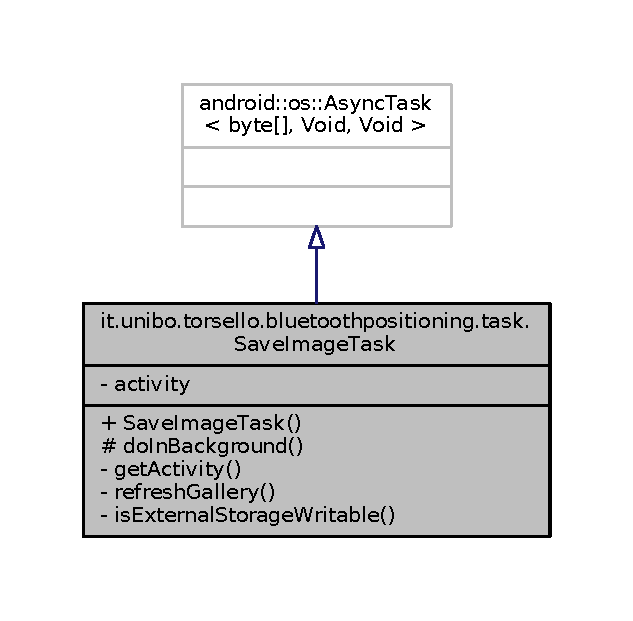
\includegraphics[width=304pt]{classit_1_1unibo_1_1torsello_1_1bluetoothpositioning_1_1task_1_1SaveImageTask__inherit__graph}
\end{center}
\end{figure}


Diagramma di collaborazione per it.\+unibo.\+torsello.\+bluetoothpositioning.\+task.\+Save\+Image\+Task\+:
\nopagebreak
\begin{figure}[H]
\begin{center}
\leavevmode
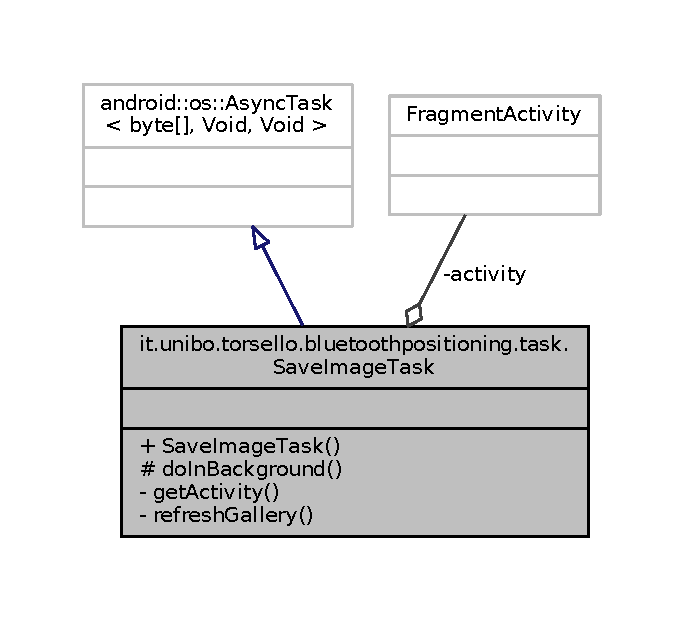
\includegraphics[width=328pt]{classit_1_1unibo_1_1torsello_1_1bluetoothpositioning_1_1task_1_1SaveImageTask__coll__graph}
\end{center}
\end{figure}
\subsubsection*{Membri pubblici}
\begin{DoxyCompactItemize}
\item 
\hyperlink{classit_1_1unibo_1_1torsello_1_1bluetoothpositioning_1_1task_1_1SaveImageTask_a73b35fbe1482ff046cc46ce21440824e_a73b35fbe1482ff046cc46ce21440824e}{Save\+Image\+Task} (Fragment\+Activity fragment\+Activity)
\end{DoxyCompactItemize}
\subsubsection*{Membri protetti}
\begin{DoxyCompactItemize}
\item 
Void \hyperlink{classit_1_1unibo_1_1torsello_1_1bluetoothpositioning_1_1task_1_1SaveImageTask_acb2bd5f71fddebe88763fef50932beeb_acb2bd5f71fddebe88763fef50932beeb}{do\+In\+Background} (byte\mbox{[}$\,$\mbox{]}... data)
\end{DoxyCompactItemize}
\subsubsection*{Membri privati}
\begin{DoxyCompactItemize}
\item 
Fragment\+Activity \hyperlink{classit_1_1unibo_1_1torsello_1_1bluetoothpositioning_1_1task_1_1SaveImageTask_a6fda270f42937b64e3767644e7dd63a5_a6fda270f42937b64e3767644e7dd63a5}{get\+Activity} ()
\item 
void \hyperlink{classit_1_1unibo_1_1torsello_1_1bluetoothpositioning_1_1task_1_1SaveImageTask_a813b3e0d75f59558de551aa6251e3d08_a813b3e0d75f59558de551aa6251e3d08}{refresh\+Gallery} (File file)
\end{DoxyCompactItemize}
\subsubsection*{Attributi privati}
\begin{DoxyCompactItemize}
\item 
Fragment\+Activity \hyperlink{classit_1_1unibo_1_1torsello_1_1bluetoothpositioning_1_1task_1_1SaveImageTask_a340aca6a2cdcfbf41aed236588669203_a340aca6a2cdcfbf41aed236588669203}{activity}
\end{DoxyCompactItemize}


\subsubsection{Descrizione dettagliata}
Created by Federico Torsello. \href{mailto:federico.torsello@studio.unibo.it}{\tt federico.\+torsello@studio.\+unibo.\+it} 

\subsubsection{Documentazione dei costruttori e dei distruttori}
\hypertarget{classit_1_1unibo_1_1torsello_1_1bluetoothpositioning_1_1task_1_1SaveImageTask_a73b35fbe1482ff046cc46ce21440824e_a73b35fbe1482ff046cc46ce21440824e}{}\label{classit_1_1unibo_1_1torsello_1_1bluetoothpositioning_1_1task_1_1SaveImageTask_a73b35fbe1482ff046cc46ce21440824e_a73b35fbe1482ff046cc46ce21440824e} 
\index{it\+::unibo\+::torsello\+::bluetoothpositioning\+::task\+::\+Save\+Image\+Task@{it\+::unibo\+::torsello\+::bluetoothpositioning\+::task\+::\+Save\+Image\+Task}!Save\+Image\+Task@{Save\+Image\+Task}}
\index{Save\+Image\+Task@{Save\+Image\+Task}!it\+::unibo\+::torsello\+::bluetoothpositioning\+::task\+::\+Save\+Image\+Task@{it\+::unibo\+::torsello\+::bluetoothpositioning\+::task\+::\+Save\+Image\+Task}}
\paragraph{\texorpdfstring{Save\+Image\+Task()}{SaveImageTask()}}
{\footnotesize\ttfamily it.\+unibo.\+torsello.\+bluetoothpositioning.\+task.\+Save\+Image\+Task.\+Save\+Image\+Task (\begin{DoxyParamCaption}\item[{Fragment\+Activity}]{fragment\+Activity }\end{DoxyParamCaption})}


\begin{DoxyCode}
26                                                             \{
27         this.\hyperlink{classit_1_1unibo_1_1torsello_1_1bluetoothpositioning_1_1task_1_1SaveImageTask_a340aca6a2cdcfbf41aed236588669203_a340aca6a2cdcfbf41aed236588669203}{activity} = fragmentActivity;
28     \}
\end{DoxyCode}


\subsubsection{Documentazione delle funzioni membro}
\hypertarget{classit_1_1unibo_1_1torsello_1_1bluetoothpositioning_1_1task_1_1SaveImageTask_acb2bd5f71fddebe88763fef50932beeb_acb2bd5f71fddebe88763fef50932beeb}{}\label{classit_1_1unibo_1_1torsello_1_1bluetoothpositioning_1_1task_1_1SaveImageTask_acb2bd5f71fddebe88763fef50932beeb_acb2bd5f71fddebe88763fef50932beeb} 
\index{it\+::unibo\+::torsello\+::bluetoothpositioning\+::task\+::\+Save\+Image\+Task@{it\+::unibo\+::torsello\+::bluetoothpositioning\+::task\+::\+Save\+Image\+Task}!do\+In\+Background@{do\+In\+Background}}
\index{do\+In\+Background@{do\+In\+Background}!it\+::unibo\+::torsello\+::bluetoothpositioning\+::task\+::\+Save\+Image\+Task@{it\+::unibo\+::torsello\+::bluetoothpositioning\+::task\+::\+Save\+Image\+Task}}
\paragraph{\texorpdfstring{do\+In\+Background()}{doInBackground()}}
{\footnotesize\ttfamily Void it.\+unibo.\+torsello.\+bluetoothpositioning.\+task.\+Save\+Image\+Task.\+do\+In\+Background (\begin{DoxyParamCaption}\item[{byte... \mbox{[}$\,$\mbox{]}}]{data }\end{DoxyParamCaption})\hspace{0.3cm}{\ttfamily [protected]}}


\begin{DoxyCode}
35                                                   \{
36 
37         \textcolor{comment}{// Write to SD Card}
38         \textcolor{keywordflow}{try} \{
39             File sdCard = Environment.getExternalStorageDirectory();
40             File dir = \textcolor{keyword}{new} File(sdCard.getAbsolutePath() + \textcolor{stringliteral}{"/"} + \hyperlink{classit_1_1unibo_1_1torsello_1_1bluetoothpositioning_1_1task_1_1SaveImageTask_a6fda270f42937b64e3767644e7dd63a5_a6fda270f42937b64e3767644e7dd63a5}{getActivity}().getString(R.
      string.app\_name));
41             dir.mkdirs();
42 
43             String fileName = String.format(Locale.getDefault(), \textcolor{stringliteral}{"%d.jpg"}, System.currentTimeMillis());
44             File outFile = \textcolor{keyword}{new} File(dir, fileName);
45 
46             FileOutputStream outStream = \textcolor{keyword}{new} FileOutputStream(outFile);
47             outStream.write(data[0]);
48             outStream.flush();
49             outStream.close();
50 
51             \hyperlink{classit_1_1unibo_1_1torsello_1_1bluetoothpositioning_1_1task_1_1SaveImageTask_a813b3e0d75f59558de551aa6251e3d08_a813b3e0d75f59558de551aa6251e3d08}{refreshGallery}(outFile);
52         \} \textcolor{keywordflow}{catch} (IOException e) \{
53             e.printStackTrace();
54         \}
55         \textcolor{keywordflow}{return} null;
56     \}
\end{DoxyCode}
\hypertarget{classit_1_1unibo_1_1torsello_1_1bluetoothpositioning_1_1task_1_1SaveImageTask_a6fda270f42937b64e3767644e7dd63a5_a6fda270f42937b64e3767644e7dd63a5}{}\label{classit_1_1unibo_1_1torsello_1_1bluetoothpositioning_1_1task_1_1SaveImageTask_a6fda270f42937b64e3767644e7dd63a5_a6fda270f42937b64e3767644e7dd63a5} 
\index{it\+::unibo\+::torsello\+::bluetoothpositioning\+::task\+::\+Save\+Image\+Task@{it\+::unibo\+::torsello\+::bluetoothpositioning\+::task\+::\+Save\+Image\+Task}!get\+Activity@{get\+Activity}}
\index{get\+Activity@{get\+Activity}!it\+::unibo\+::torsello\+::bluetoothpositioning\+::task\+::\+Save\+Image\+Task@{it\+::unibo\+::torsello\+::bluetoothpositioning\+::task\+::\+Save\+Image\+Task}}
\paragraph{\texorpdfstring{get\+Activity()}{getActivity()}}
{\footnotesize\ttfamily Fragment\+Activity it.\+unibo.\+torsello.\+bluetoothpositioning.\+task.\+Save\+Image\+Task.\+get\+Activity (\begin{DoxyParamCaption}{ }\end{DoxyParamCaption})\hspace{0.3cm}{\ttfamily [private]}}


\begin{DoxyCode}
30                                            \{
31         \textcolor{keywordflow}{return} \hyperlink{classit_1_1unibo_1_1torsello_1_1bluetoothpositioning_1_1task_1_1SaveImageTask_a340aca6a2cdcfbf41aed236588669203_a340aca6a2cdcfbf41aed236588669203}{activity};
32     \}
\end{DoxyCode}
\hypertarget{classit_1_1unibo_1_1torsello_1_1bluetoothpositioning_1_1task_1_1SaveImageTask_a813b3e0d75f59558de551aa6251e3d08_a813b3e0d75f59558de551aa6251e3d08}{}\label{classit_1_1unibo_1_1torsello_1_1bluetoothpositioning_1_1task_1_1SaveImageTask_a813b3e0d75f59558de551aa6251e3d08_a813b3e0d75f59558de551aa6251e3d08} 
\index{it\+::unibo\+::torsello\+::bluetoothpositioning\+::task\+::\+Save\+Image\+Task@{it\+::unibo\+::torsello\+::bluetoothpositioning\+::task\+::\+Save\+Image\+Task}!refresh\+Gallery@{refresh\+Gallery}}
\index{refresh\+Gallery@{refresh\+Gallery}!it\+::unibo\+::torsello\+::bluetoothpositioning\+::task\+::\+Save\+Image\+Task@{it\+::unibo\+::torsello\+::bluetoothpositioning\+::task\+::\+Save\+Image\+Task}}
\paragraph{\texorpdfstring{refresh\+Gallery()}{refreshGallery()}}
{\footnotesize\ttfamily void it.\+unibo.\+torsello.\+bluetoothpositioning.\+task.\+Save\+Image\+Task.\+refresh\+Gallery (\begin{DoxyParamCaption}\item[{File}]{file }\end{DoxyParamCaption})\hspace{0.3cm}{\ttfamily [private]}}


\begin{DoxyCode}
58                                            \{
59         \textcolor{keywordflow}{if} (file != null)\{
60             Intent mediaScanIntent = \textcolor{keyword}{new} Intent(Intent.ACTION\_MEDIA\_SCANNER\_SCAN\_FILE);
61             mediaScanIntent.setData(Uri.fromFile(file));
62             \hyperlink{classit_1_1unibo_1_1torsello_1_1bluetoothpositioning_1_1task_1_1SaveImageTask_a6fda270f42937b64e3767644e7dd63a5_a6fda270f42937b64e3767644e7dd63a5}{getActivity}().sendBroadcast(mediaScanIntent);
63 
64             Snackbar.make(\hyperlink{classit_1_1unibo_1_1torsello_1_1bluetoothpositioning_1_1task_1_1SaveImageTask_a6fda270f42937b64e3767644e7dd63a5_a6fda270f42937b64e3767644e7dd63a5}{getActivity}().findViewById(R.id.fab),
65                     \textcolor{stringliteral}{"Your picture has been saved"}, Snackbar.LENGTH\_SHORT).show();
66         \} \textcolor{keywordflow}{else} \{
67             Snackbar.make(\hyperlink{classit_1_1unibo_1_1torsello_1_1bluetoothpositioning_1_1task_1_1SaveImageTask_a6fda270f42937b64e3767644e7dd63a5_a6fda270f42937b64e3767644e7dd63a5}{getActivity}().findViewById(R.id.fab),
68                         \textcolor{stringliteral}{"Image retrieval failed"}, Snackbar.LENGTH\_SHORT).show();
69         \}
70     \}
\end{DoxyCode}


\subsubsection{Documentazione dei membri dato}
\hypertarget{classit_1_1unibo_1_1torsello_1_1bluetoothpositioning_1_1task_1_1SaveImageTask_a340aca6a2cdcfbf41aed236588669203_a340aca6a2cdcfbf41aed236588669203}{}\label{classit_1_1unibo_1_1torsello_1_1bluetoothpositioning_1_1task_1_1SaveImageTask_a340aca6a2cdcfbf41aed236588669203_a340aca6a2cdcfbf41aed236588669203} 
\index{it\+::unibo\+::torsello\+::bluetoothpositioning\+::task\+::\+Save\+Image\+Task@{it\+::unibo\+::torsello\+::bluetoothpositioning\+::task\+::\+Save\+Image\+Task}!activity@{activity}}
\index{activity@{activity}!it\+::unibo\+::torsello\+::bluetoothpositioning\+::task\+::\+Save\+Image\+Task@{it\+::unibo\+::torsello\+::bluetoothpositioning\+::task\+::\+Save\+Image\+Task}}
\paragraph{\texorpdfstring{activity}{activity}}
{\footnotesize\ttfamily Fragment\+Activity it.\+unibo.\+torsello.\+bluetoothpositioning.\+task.\+Save\+Image\+Task.\+activity\hspace{0.3cm}{\ttfamily [private]}}



La documentazione per questa classe è stata generata a partire dal seguente file\+:\begin{DoxyCompactItemize}
\item 
\hyperlink{SaveImageTask_8java}{Save\+Image\+Task.\+java}\end{DoxyCompactItemize}

\hypertarget{classit_1_1unibo_1_1torsello_1_1bluetoothpositioning_1_1constant_1_1SettingConstants}{}\subsection{Riferimenti per la classe it.\+unibo.\+torsello.\+bluetoothpositioning.\+constant.\+Setting\+Constants}
\label{classit_1_1unibo_1_1torsello_1_1bluetoothpositioning_1_1constant_1_1SettingConstants}\index{it.\+unibo.\+torsello.\+bluetoothpositioning.\+constant.\+Setting\+Constants@{it.\+unibo.\+torsello.\+bluetoothpositioning.\+constant.\+Setting\+Constants}}


Diagramma di collaborazione per it.\+unibo.\+torsello.\+bluetoothpositioning.\+constant.\+Setting\+Constants\+:
\nopagebreak
\begin{figure}[H]
\begin{center}
\leavevmode
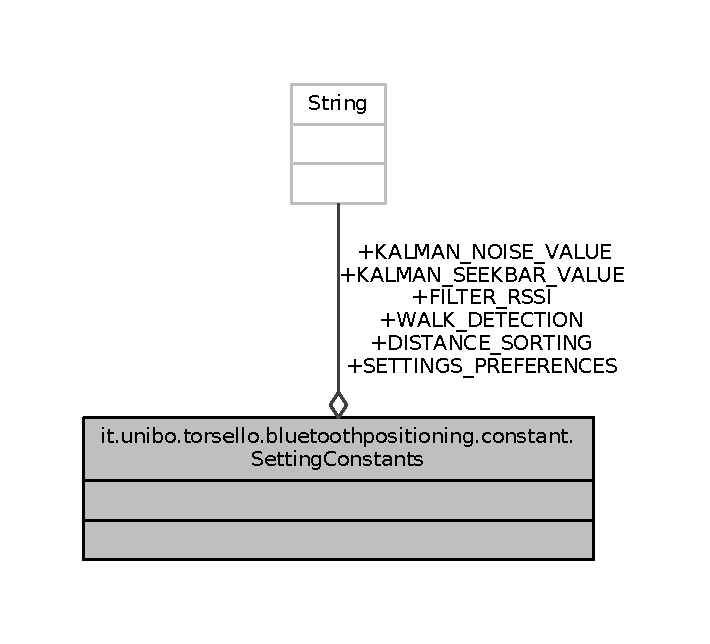
\includegraphics[width=342pt]{classit_1_1unibo_1_1torsello_1_1bluetoothpositioning_1_1constant_1_1SettingConstants__coll__graph}
\end{center}
\end{figure}
\subsubsection*{Attributi pubblici statici}
\begin{DoxyCompactItemize}
\item 
static final String \hyperlink{classit_1_1unibo_1_1torsello_1_1bluetoothpositioning_1_1constant_1_1SettingConstants_ae1b406c787a7efb87d585d5c8b80493d_ae1b406c787a7efb87d585d5c8b80493d}{S\+E\+T\+T\+I\+N\+G\+S\+\_\+\+P\+R\+E\+F\+E\+R\+E\+N\+C\+ES} = \char`\"{}settings\+\_\+preferences\char`\"{}
\item 
static final String \hyperlink{classit_1_1unibo_1_1torsello_1_1bluetoothpositioning_1_1constant_1_1SettingConstants_a60a6d73ab1d42653b8a0c5b10c1c80c5_a60a6d73ab1d42653b8a0c5b10c1c80c5}{F\+I\+L\+T\+E\+R\+\_\+\+R\+S\+SI} = \char`\"{}filter\+\_\+rssi\char`\"{}
\item 
static final String \hyperlink{classit_1_1unibo_1_1torsello_1_1bluetoothpositioning_1_1constant_1_1SettingConstants_ad8f1f7986a4558736769604d606f53a1_ad8f1f7986a4558736769604d606f53a1}{A\+R\+M\+A\+\_\+\+O\+P\+T\+I\+ON} = \char`\"{}arma\+\_\+option\char`\"{}
\item 
static final String \hyperlink{classit_1_1unibo_1_1torsello_1_1bluetoothpositioning_1_1constant_1_1SettingConstants_a2c0b004552568f9813696b26b89b840c_a2c0b004552568f9813696b26b89b840c}{A\+V\+G\+\_\+\+O\+P\+T\+I\+ON} = \char`\"{}avg\+\_\+option\char`\"{}
\item 
static final String \hyperlink{classit_1_1unibo_1_1torsello_1_1bluetoothpositioning_1_1constant_1_1SettingConstants_a7ba43b29e467efb129d86c917734c94b_a7ba43b29e467efb129d86c917734c94b}{K\+A\+L\+M\+A\+N\+\_\+\+S\+E\+E\+K\+B\+A\+R\+\_\+\+V\+A\+L\+UE} = \char`\"{}kalman\+\_\+filter\+\_\+seek\+\_\+value\char`\"{}
\item 
static final String \hyperlink{classit_1_1unibo_1_1torsello_1_1bluetoothpositioning_1_1constant_1_1SettingConstants_a2751989834b974103dda417fb8b10337_a2751989834b974103dda417fb8b10337}{K\+A\+L\+M\+A\+N\+\_\+\+N\+O\+I\+S\+E\+\_\+\+V\+A\+L\+UE} = \char`\"{}kalman\+\_\+filter\+\_\+noise\+\_\+value\char`\"{}
\item 
static final String \hyperlink{classit_1_1unibo_1_1torsello_1_1bluetoothpositioning_1_1constant_1_1SettingConstants_a974ee83a6959f7965c5fa27ac8dc0798_a974ee83a6959f7965c5fa27ac8dc0798}{K\+A\+L\+M\+A\+N\+\_\+\+F\+I\+L\+T\+E\+R\+\_\+\+E\+N\+A\+B\+L\+ED} = \char`\"{}kalma\+\_\+filrer\+\_\+enabled\char`\"{}
\item 
static final String \hyperlink{classit_1_1unibo_1_1torsello_1_1bluetoothpositioning_1_1constant_1_1SettingConstants_ad86af94213ec3f11669289c4972c7658_ad86af94213ec3f11669289c4972c7658}{D\+I\+S\+T\+A\+N\+C\+E\+\_\+\+S\+O\+R\+T\+I\+NG} = \char`\"{}distance\+\_\+sorting\+\_\+selected\char`\"{}
\end{DoxyCompactItemize}


\subsubsection{Descrizione dettagliata}
Created by Federico Torsello. \href{mailto:federico.torsello@studio.unibo.it}{\tt federico.\+torsello@studio.\+unibo.\+it} 

A class containing constants for the Shared\+Preference objects. 

\subsubsection{Documentazione dei membri dato}
\hypertarget{classit_1_1unibo_1_1torsello_1_1bluetoothpositioning_1_1constant_1_1SettingConstants_ad8f1f7986a4558736769604d606f53a1_ad8f1f7986a4558736769604d606f53a1}{}\label{classit_1_1unibo_1_1torsello_1_1bluetoothpositioning_1_1constant_1_1SettingConstants_ad8f1f7986a4558736769604d606f53a1_ad8f1f7986a4558736769604d606f53a1} 
\index{it\+::unibo\+::torsello\+::bluetoothpositioning\+::constant\+::\+Setting\+Constants@{it\+::unibo\+::torsello\+::bluetoothpositioning\+::constant\+::\+Setting\+Constants}!A\+R\+M\+A\+\_\+\+O\+P\+T\+I\+ON@{A\+R\+M\+A\+\_\+\+O\+P\+T\+I\+ON}}
\index{A\+R\+M\+A\+\_\+\+O\+P\+T\+I\+ON@{A\+R\+M\+A\+\_\+\+O\+P\+T\+I\+ON}!it\+::unibo\+::torsello\+::bluetoothpositioning\+::constant\+::\+Setting\+Constants@{it\+::unibo\+::torsello\+::bluetoothpositioning\+::constant\+::\+Setting\+Constants}}
\paragraph{\texorpdfstring{A\+R\+M\+A\+\_\+\+O\+P\+T\+I\+ON}{ARMA\_OPTION}}
{\footnotesize\ttfamily final String it.\+unibo.\+torsello.\+bluetoothpositioning.\+constant.\+Setting\+Constants.\+A\+R\+M\+A\+\_\+\+O\+P\+T\+I\+ON = \char`\"{}arma\+\_\+option\char`\"{}\hspace{0.3cm}{\ttfamily [static]}}

\hypertarget{classit_1_1unibo_1_1torsello_1_1bluetoothpositioning_1_1constant_1_1SettingConstants_a2c0b004552568f9813696b26b89b840c_a2c0b004552568f9813696b26b89b840c}{}\label{classit_1_1unibo_1_1torsello_1_1bluetoothpositioning_1_1constant_1_1SettingConstants_a2c0b004552568f9813696b26b89b840c_a2c0b004552568f9813696b26b89b840c} 
\index{it\+::unibo\+::torsello\+::bluetoothpositioning\+::constant\+::\+Setting\+Constants@{it\+::unibo\+::torsello\+::bluetoothpositioning\+::constant\+::\+Setting\+Constants}!A\+V\+G\+\_\+\+O\+P\+T\+I\+ON@{A\+V\+G\+\_\+\+O\+P\+T\+I\+ON}}
\index{A\+V\+G\+\_\+\+O\+P\+T\+I\+ON@{A\+V\+G\+\_\+\+O\+P\+T\+I\+ON}!it\+::unibo\+::torsello\+::bluetoothpositioning\+::constant\+::\+Setting\+Constants@{it\+::unibo\+::torsello\+::bluetoothpositioning\+::constant\+::\+Setting\+Constants}}
\paragraph{\texorpdfstring{A\+V\+G\+\_\+\+O\+P\+T\+I\+ON}{AVG\_OPTION}}
{\footnotesize\ttfamily final String it.\+unibo.\+torsello.\+bluetoothpositioning.\+constant.\+Setting\+Constants.\+A\+V\+G\+\_\+\+O\+P\+T\+I\+ON = \char`\"{}avg\+\_\+option\char`\"{}\hspace{0.3cm}{\ttfamily [static]}}

\hypertarget{classit_1_1unibo_1_1torsello_1_1bluetoothpositioning_1_1constant_1_1SettingConstants_ad86af94213ec3f11669289c4972c7658_ad86af94213ec3f11669289c4972c7658}{}\label{classit_1_1unibo_1_1torsello_1_1bluetoothpositioning_1_1constant_1_1SettingConstants_ad86af94213ec3f11669289c4972c7658_ad86af94213ec3f11669289c4972c7658} 
\index{it\+::unibo\+::torsello\+::bluetoothpositioning\+::constant\+::\+Setting\+Constants@{it\+::unibo\+::torsello\+::bluetoothpositioning\+::constant\+::\+Setting\+Constants}!D\+I\+S\+T\+A\+N\+C\+E\+\_\+\+S\+O\+R\+T\+I\+NG@{D\+I\+S\+T\+A\+N\+C\+E\+\_\+\+S\+O\+R\+T\+I\+NG}}
\index{D\+I\+S\+T\+A\+N\+C\+E\+\_\+\+S\+O\+R\+T\+I\+NG@{D\+I\+S\+T\+A\+N\+C\+E\+\_\+\+S\+O\+R\+T\+I\+NG}!it\+::unibo\+::torsello\+::bluetoothpositioning\+::constant\+::\+Setting\+Constants@{it\+::unibo\+::torsello\+::bluetoothpositioning\+::constant\+::\+Setting\+Constants}}
\paragraph{\texorpdfstring{D\+I\+S\+T\+A\+N\+C\+E\+\_\+\+S\+O\+R\+T\+I\+NG}{DISTANCE\_SORTING}}
{\footnotesize\ttfamily final String it.\+unibo.\+torsello.\+bluetoothpositioning.\+constant.\+Setting\+Constants.\+D\+I\+S\+T\+A\+N\+C\+E\+\_\+\+S\+O\+R\+T\+I\+NG = \char`\"{}distance\+\_\+sorting\+\_\+selected\char`\"{}\hspace{0.3cm}{\ttfamily [static]}}

\hypertarget{classit_1_1unibo_1_1torsello_1_1bluetoothpositioning_1_1constant_1_1SettingConstants_a60a6d73ab1d42653b8a0c5b10c1c80c5_a60a6d73ab1d42653b8a0c5b10c1c80c5}{}\label{classit_1_1unibo_1_1torsello_1_1bluetoothpositioning_1_1constant_1_1SettingConstants_a60a6d73ab1d42653b8a0c5b10c1c80c5_a60a6d73ab1d42653b8a0c5b10c1c80c5} 
\index{it\+::unibo\+::torsello\+::bluetoothpositioning\+::constant\+::\+Setting\+Constants@{it\+::unibo\+::torsello\+::bluetoothpositioning\+::constant\+::\+Setting\+Constants}!F\+I\+L\+T\+E\+R\+\_\+\+R\+S\+SI@{F\+I\+L\+T\+E\+R\+\_\+\+R\+S\+SI}}
\index{F\+I\+L\+T\+E\+R\+\_\+\+R\+S\+SI@{F\+I\+L\+T\+E\+R\+\_\+\+R\+S\+SI}!it\+::unibo\+::torsello\+::bluetoothpositioning\+::constant\+::\+Setting\+Constants@{it\+::unibo\+::torsello\+::bluetoothpositioning\+::constant\+::\+Setting\+Constants}}
\paragraph{\texorpdfstring{F\+I\+L\+T\+E\+R\+\_\+\+R\+S\+SI}{FILTER\_RSSI}}
{\footnotesize\ttfamily final String it.\+unibo.\+torsello.\+bluetoothpositioning.\+constant.\+Setting\+Constants.\+F\+I\+L\+T\+E\+R\+\_\+\+R\+S\+SI = \char`\"{}filter\+\_\+rssi\char`\"{}\hspace{0.3cm}{\ttfamily [static]}}

\hypertarget{classit_1_1unibo_1_1torsello_1_1bluetoothpositioning_1_1constant_1_1SettingConstants_a974ee83a6959f7965c5fa27ac8dc0798_a974ee83a6959f7965c5fa27ac8dc0798}{}\label{classit_1_1unibo_1_1torsello_1_1bluetoothpositioning_1_1constant_1_1SettingConstants_a974ee83a6959f7965c5fa27ac8dc0798_a974ee83a6959f7965c5fa27ac8dc0798} 
\index{it\+::unibo\+::torsello\+::bluetoothpositioning\+::constant\+::\+Setting\+Constants@{it\+::unibo\+::torsello\+::bluetoothpositioning\+::constant\+::\+Setting\+Constants}!K\+A\+L\+M\+A\+N\+\_\+\+F\+I\+L\+T\+E\+R\+\_\+\+E\+N\+A\+B\+L\+ED@{K\+A\+L\+M\+A\+N\+\_\+\+F\+I\+L\+T\+E\+R\+\_\+\+E\+N\+A\+B\+L\+ED}}
\index{K\+A\+L\+M\+A\+N\+\_\+\+F\+I\+L\+T\+E\+R\+\_\+\+E\+N\+A\+B\+L\+ED@{K\+A\+L\+M\+A\+N\+\_\+\+F\+I\+L\+T\+E\+R\+\_\+\+E\+N\+A\+B\+L\+ED}!it\+::unibo\+::torsello\+::bluetoothpositioning\+::constant\+::\+Setting\+Constants@{it\+::unibo\+::torsello\+::bluetoothpositioning\+::constant\+::\+Setting\+Constants}}
\paragraph{\texorpdfstring{K\+A\+L\+M\+A\+N\+\_\+\+F\+I\+L\+T\+E\+R\+\_\+\+E\+N\+A\+B\+L\+ED}{KALMAN\_FILTER\_ENABLED}}
{\footnotesize\ttfamily final String it.\+unibo.\+torsello.\+bluetoothpositioning.\+constant.\+Setting\+Constants.\+K\+A\+L\+M\+A\+N\+\_\+\+F\+I\+L\+T\+E\+R\+\_\+\+E\+N\+A\+B\+L\+ED = \char`\"{}kalma\+\_\+filrer\+\_\+enabled\char`\"{}\hspace{0.3cm}{\ttfamily [static]}}

\hypertarget{classit_1_1unibo_1_1torsello_1_1bluetoothpositioning_1_1constant_1_1SettingConstants_a2751989834b974103dda417fb8b10337_a2751989834b974103dda417fb8b10337}{}\label{classit_1_1unibo_1_1torsello_1_1bluetoothpositioning_1_1constant_1_1SettingConstants_a2751989834b974103dda417fb8b10337_a2751989834b974103dda417fb8b10337} 
\index{it\+::unibo\+::torsello\+::bluetoothpositioning\+::constant\+::\+Setting\+Constants@{it\+::unibo\+::torsello\+::bluetoothpositioning\+::constant\+::\+Setting\+Constants}!K\+A\+L\+M\+A\+N\+\_\+\+N\+O\+I\+S\+E\+\_\+\+V\+A\+L\+UE@{K\+A\+L\+M\+A\+N\+\_\+\+N\+O\+I\+S\+E\+\_\+\+V\+A\+L\+UE}}
\index{K\+A\+L\+M\+A\+N\+\_\+\+N\+O\+I\+S\+E\+\_\+\+V\+A\+L\+UE@{K\+A\+L\+M\+A\+N\+\_\+\+N\+O\+I\+S\+E\+\_\+\+V\+A\+L\+UE}!it\+::unibo\+::torsello\+::bluetoothpositioning\+::constant\+::\+Setting\+Constants@{it\+::unibo\+::torsello\+::bluetoothpositioning\+::constant\+::\+Setting\+Constants}}
\paragraph{\texorpdfstring{K\+A\+L\+M\+A\+N\+\_\+\+N\+O\+I\+S\+E\+\_\+\+V\+A\+L\+UE}{KALMAN\_NOISE\_VALUE}}
{\footnotesize\ttfamily final String it.\+unibo.\+torsello.\+bluetoothpositioning.\+constant.\+Setting\+Constants.\+K\+A\+L\+M\+A\+N\+\_\+\+N\+O\+I\+S\+E\+\_\+\+V\+A\+L\+UE = \char`\"{}kalman\+\_\+filter\+\_\+noise\+\_\+value\char`\"{}\hspace{0.3cm}{\ttfamily [static]}}

\hypertarget{classit_1_1unibo_1_1torsello_1_1bluetoothpositioning_1_1constant_1_1SettingConstants_a7ba43b29e467efb129d86c917734c94b_a7ba43b29e467efb129d86c917734c94b}{}\label{classit_1_1unibo_1_1torsello_1_1bluetoothpositioning_1_1constant_1_1SettingConstants_a7ba43b29e467efb129d86c917734c94b_a7ba43b29e467efb129d86c917734c94b} 
\index{it\+::unibo\+::torsello\+::bluetoothpositioning\+::constant\+::\+Setting\+Constants@{it\+::unibo\+::torsello\+::bluetoothpositioning\+::constant\+::\+Setting\+Constants}!K\+A\+L\+M\+A\+N\+\_\+\+S\+E\+E\+K\+B\+A\+R\+\_\+\+V\+A\+L\+UE@{K\+A\+L\+M\+A\+N\+\_\+\+S\+E\+E\+K\+B\+A\+R\+\_\+\+V\+A\+L\+UE}}
\index{K\+A\+L\+M\+A\+N\+\_\+\+S\+E\+E\+K\+B\+A\+R\+\_\+\+V\+A\+L\+UE@{K\+A\+L\+M\+A\+N\+\_\+\+S\+E\+E\+K\+B\+A\+R\+\_\+\+V\+A\+L\+UE}!it\+::unibo\+::torsello\+::bluetoothpositioning\+::constant\+::\+Setting\+Constants@{it\+::unibo\+::torsello\+::bluetoothpositioning\+::constant\+::\+Setting\+Constants}}
\paragraph{\texorpdfstring{K\+A\+L\+M\+A\+N\+\_\+\+S\+E\+E\+K\+B\+A\+R\+\_\+\+V\+A\+L\+UE}{KALMAN\_SEEKBAR\_VALUE}}
{\footnotesize\ttfamily final String it.\+unibo.\+torsello.\+bluetoothpositioning.\+constant.\+Setting\+Constants.\+K\+A\+L\+M\+A\+N\+\_\+\+S\+E\+E\+K\+B\+A\+R\+\_\+\+V\+A\+L\+UE = \char`\"{}kalman\+\_\+filter\+\_\+seek\+\_\+value\char`\"{}\hspace{0.3cm}{\ttfamily [static]}}

\hypertarget{classit_1_1unibo_1_1torsello_1_1bluetoothpositioning_1_1constant_1_1SettingConstants_ae1b406c787a7efb87d585d5c8b80493d_ae1b406c787a7efb87d585d5c8b80493d}{}\label{classit_1_1unibo_1_1torsello_1_1bluetoothpositioning_1_1constant_1_1SettingConstants_ae1b406c787a7efb87d585d5c8b80493d_ae1b406c787a7efb87d585d5c8b80493d} 
\index{it\+::unibo\+::torsello\+::bluetoothpositioning\+::constant\+::\+Setting\+Constants@{it\+::unibo\+::torsello\+::bluetoothpositioning\+::constant\+::\+Setting\+Constants}!S\+E\+T\+T\+I\+N\+G\+S\+\_\+\+P\+R\+E\+F\+E\+R\+E\+N\+C\+ES@{S\+E\+T\+T\+I\+N\+G\+S\+\_\+\+P\+R\+E\+F\+E\+R\+E\+N\+C\+ES}}
\index{S\+E\+T\+T\+I\+N\+G\+S\+\_\+\+P\+R\+E\+F\+E\+R\+E\+N\+C\+ES@{S\+E\+T\+T\+I\+N\+G\+S\+\_\+\+P\+R\+E\+F\+E\+R\+E\+N\+C\+ES}!it\+::unibo\+::torsello\+::bluetoothpositioning\+::constant\+::\+Setting\+Constants@{it\+::unibo\+::torsello\+::bluetoothpositioning\+::constant\+::\+Setting\+Constants}}
\paragraph{\texorpdfstring{S\+E\+T\+T\+I\+N\+G\+S\+\_\+\+P\+R\+E\+F\+E\+R\+E\+N\+C\+ES}{SETTINGS\_PREFERENCES}}
{\footnotesize\ttfamily final String it.\+unibo.\+torsello.\+bluetoothpositioning.\+constant.\+Setting\+Constants.\+S\+E\+T\+T\+I\+N\+G\+S\+\_\+\+P\+R\+E\+F\+E\+R\+E\+N\+C\+ES = \char`\"{}settings\+\_\+preferences\char`\"{}\hspace{0.3cm}{\ttfamily [static]}}



La documentazione per questa classe è stata generata a partire dal seguente file\+:\begin{DoxyCompactItemize}
\item 
\hyperlink{SettingConstants_8java}{Setting\+Constants.\+java}\end{DoxyCompactItemize}

\hypertarget{classit_1_1unibo_1_1torsello_1_1bluetoothpositioning_1_1fragment_1_1SettingsFragment}{}\subsection{Riferimenti per la classe it.\+unibo.\+torsello.\+bluetoothpositioning.\+fragment.\+Settings\+Fragment}
\label{classit_1_1unibo_1_1torsello_1_1bluetoothpositioning_1_1fragment_1_1SettingsFragment}\index{it.\+unibo.\+torsello.\+bluetoothpositioning.\+fragment.\+Settings\+Fragment@{it.\+unibo.\+torsello.\+bluetoothpositioning.\+fragment.\+Settings\+Fragment}}


Diagramma delle classi per it.\+unibo.\+torsello.\+bluetoothpositioning.\+fragment.\+Settings\+Fragment
\nopagebreak
\begin{figure}[H]
\begin{center}
\leavevmode
\includegraphics[width=328pt]{classit_1_1unibo_1_1torsello_1_1bluetoothpositioning_1_1fragment_1_1SettingsFragment__inherit__graph}
\end{center}
\end{figure}


Diagramma di collaborazione per it.\+unibo.\+torsello.\+bluetoothpositioning.\+fragment.\+Settings\+Fragment\+:
\nopagebreak
\begin{figure}[H]
\begin{center}
\leavevmode
\includegraphics[width=350pt]{classit_1_1unibo_1_1torsello_1_1bluetoothpositioning_1_1fragment_1_1SettingsFragment__coll__graph}
\end{center}
\end{figure}
\subsubsection*{Membri pubblici}
\begin{DoxyCompactItemize}
\item 
void \hyperlink{classit_1_1unibo_1_1torsello_1_1bluetoothpositioning_1_1fragment_1_1SettingsFragment_a7de90efb25e655078f5f8984f7c6d628_a7de90efb25e655078f5f8984f7c6d628}{on\+Create} (Bundle saved\+Instance\+State)
\item 
View \hyperlink{classit_1_1unibo_1_1torsello_1_1bluetoothpositioning_1_1fragment_1_1SettingsFragment_ac1c9d47777382cc2c74b7b1cf3d6ccd7_ac1c9d47777382cc2c74b7b1cf3d6ccd7}{on\+Create\+View} (Layout\+Inflater inflater, View\+Group container, Bundle saved\+Instance\+State)
\end{DoxyCompactItemize}
\subsubsection*{Membri pubblici statici}
\begin{DoxyCompactItemize}
\item 
static \hyperlink{classit_1_1unibo_1_1torsello_1_1bluetoothpositioning_1_1fragment_1_1SettingsFragment}{Settings\+Fragment} \hyperlink{classit_1_1unibo_1_1torsello_1_1bluetoothpositioning_1_1fragment_1_1SettingsFragment_a4eb69c78cde2ba119eb62453688280f5_a4eb69c78cde2ba119eb62453688280f5}{new\+Instance} ()
\end{DoxyCompactItemize}
\subsubsection*{Membri privati}
\begin{DoxyCompactItemize}
\item 
void \hyperlink{classit_1_1unibo_1_1torsello_1_1bluetoothpositioning_1_1fragment_1_1SettingsFragment_a84057f1633708ec85de5968ed9e7f032_a84057f1633708ec85de5968ed9e7f032}{set\+Kalman\+Filter\+Seek\+Bar} (View root)
\item 
void \hyperlink{classit_1_1unibo_1_1torsello_1_1bluetoothpositioning_1_1fragment_1_1SettingsFragment_ae16c093ba7bc137acf21dfc221cdcf56_ae16c093ba7bc137acf21dfc221cdcf56}{set\+Enabled\+Kalman\+Filter} (int progress)
\item 
void \hyperlink{classit_1_1unibo_1_1torsello_1_1bluetoothpositioning_1_1fragment_1_1SettingsFragment_a0d7b911602439aaf2a9ee4d5f9e41088_a0d7b911602439aaf2a9ee4d5f9e41088}{set\+Filtering} (View root)
\item 
void \hyperlink{classit_1_1unibo_1_1torsello_1_1bluetoothpositioning_1_1fragment_1_1SettingsFragment_a0f26c84f3a3dfffabfed1db04303b8b0_a0f26c84f3a3dfffabfed1db04303b8b0}{set\+Avg\+Option} (View root)
\item 
void \hyperlink{classit_1_1unibo_1_1torsello_1_1bluetoothpositioning_1_1fragment_1_1SettingsFragment_a093ab503fb5dc6ddb859b128b614d902_a093ab503fb5dc6ddb859b128b614d902}{set\+Arma\+Option} (View root)
\item 
void \hyperlink{classit_1_1unibo_1_1torsello_1_1bluetoothpositioning_1_1fragment_1_1SettingsFragment_ae29f0b3d6fc60f1ceeab5dcc530166c1_ae29f0b3d6fc60f1ceeab5dcc530166c1}{set\+Sorting} (View root)
\end{DoxyCompactItemize}
\subsubsection*{Membri privati statici}
\begin{DoxyCompactItemize}
\item 
static float \hyperlink{classit_1_1unibo_1_1torsello_1_1bluetoothpositioning_1_1fragment_1_1SettingsFragment_a595d859602f34ca81957a0578c1602a6_a595d859602f34ca81957a0578c1602a6}{get\+Calculated\+Noise} (int p)
\end{DoxyCompactItemize}
\subsubsection*{Attributi privati}
\begin{DoxyCompactItemize}
\item 
Shared\+Preferences \hyperlink{classit_1_1unibo_1_1torsello_1_1bluetoothpositioning_1_1fragment_1_1SettingsFragment_a52480c4d5d81ca59fe4a98ae3c623ea4_a52480c4d5d81ca59fe4a98ae3c623ea4}{preferences}
\item 
Decimal\+Format \hyperlink{classit_1_1unibo_1_1torsello_1_1bluetoothpositioning_1_1fragment_1_1SettingsFragment_af6b80a700dc80c39a56d001b68a47694_af6b80a700dc80c39a56d001b68a47694}{df}
\end{DoxyCompactItemize}
\subsubsection*{Attributi privati statici}
\begin{DoxyCompactItemize}
\item 
static final String \hyperlink{classit_1_1unibo_1_1torsello_1_1bluetoothpositioning_1_1fragment_1_1SettingsFragment_a3f3c627008cd1e176afc52642c73fd93_a3f3c627008cd1e176afc52642c73fd93}{E\+X\+T\+R\+A\+\_\+\+M\+E\+S\+S\+A\+GE} = \char`\"{}E\+X\+T\+R\+A\+\_\+\+M\+E\+S\+S\+A\+GE\char`\"{}
\end{DoxyCompactItemize}


\subsubsection{Descrizione dettagliata}
Created by Federico Torsello. \href{mailto:federico.torsello@studio.unibo.it}{\tt federico.\+torsello@studio.\+unibo.\+it} 

\subsubsection{Documentazione delle funzioni membro}
\hypertarget{classit_1_1unibo_1_1torsello_1_1bluetoothpositioning_1_1fragment_1_1SettingsFragment_a595d859602f34ca81957a0578c1602a6_a595d859602f34ca81957a0578c1602a6}{}\label{classit_1_1unibo_1_1torsello_1_1bluetoothpositioning_1_1fragment_1_1SettingsFragment_a595d859602f34ca81957a0578c1602a6_a595d859602f34ca81957a0578c1602a6} 
\index{it\+::unibo\+::torsello\+::bluetoothpositioning\+::fragment\+::\+Settings\+Fragment@{it\+::unibo\+::torsello\+::bluetoothpositioning\+::fragment\+::\+Settings\+Fragment}!get\+Calculated\+Noise@{get\+Calculated\+Noise}}
\index{get\+Calculated\+Noise@{get\+Calculated\+Noise}!it\+::unibo\+::torsello\+::bluetoothpositioning\+::fragment\+::\+Settings\+Fragment@{it\+::unibo\+::torsello\+::bluetoothpositioning\+::fragment\+::\+Settings\+Fragment}}
\paragraph{\texorpdfstring{get\+Calculated\+Noise()}{getCalculatedNoise()}}
{\footnotesize\ttfamily static float it.\+unibo.\+torsello.\+bluetoothpositioning.\+fragment.\+Settings\+Fragment.\+get\+Calculated\+Noise (\begin{DoxyParamCaption}\item[{int}]{p }\end{DoxyParamCaption})\hspace{0.3cm}{\ttfamily [static]}, {\ttfamily [private]}}


\begin{DoxyCode}
112                                                    \{
113         \textcolor{keywordtype}{double} percent = (p / 10D);
114         \textcolor{keywordtype}{double} noise = KFilterConstants.KALMAN\_NOISE\_MIN +
115                 (KFilterConstants.KALMAN\_NOISE\_MAX - KFilterConstants.KALMAN\_NOISE\_MIN) * percent;
116 
117         \textcolor{keywordflow}{return} (\textcolor{keywordtype}{float}) noise;
118 
119     \}
\end{DoxyCode}
\hypertarget{classit_1_1unibo_1_1torsello_1_1bluetoothpositioning_1_1fragment_1_1SettingsFragment_a4eb69c78cde2ba119eb62453688280f5_a4eb69c78cde2ba119eb62453688280f5}{}\label{classit_1_1unibo_1_1torsello_1_1bluetoothpositioning_1_1fragment_1_1SettingsFragment_a4eb69c78cde2ba119eb62453688280f5_a4eb69c78cde2ba119eb62453688280f5} 
\index{it\+::unibo\+::torsello\+::bluetoothpositioning\+::fragment\+::\+Settings\+Fragment@{it\+::unibo\+::torsello\+::bluetoothpositioning\+::fragment\+::\+Settings\+Fragment}!new\+Instance@{new\+Instance}}
\index{new\+Instance@{new\+Instance}!it\+::unibo\+::torsello\+::bluetoothpositioning\+::fragment\+::\+Settings\+Fragment@{it\+::unibo\+::torsello\+::bluetoothpositioning\+::fragment\+::\+Settings\+Fragment}}
\paragraph{\texorpdfstring{new\+Instance()}{newInstance()}}
{\footnotesize\ttfamily static \hyperlink{classit_1_1unibo_1_1torsello_1_1bluetoothpositioning_1_1fragment_1_1SettingsFragment}{Settings\+Fragment} it.\+unibo.\+torsello.\+bluetoothpositioning.\+fragment.\+Settings\+Fragment.\+new\+Instance (\begin{DoxyParamCaption}{ }\end{DoxyParamCaption})\hspace{0.3cm}{\ttfamily [static]}}


\begin{DoxyCode}
29                                                  \{
30         SettingsFragment fragment = \textcolor{keyword}{new} SettingsFragment();
31         Bundle args = \textcolor{keyword}{new} Bundle();
32         args.putString(\hyperlink{classit_1_1unibo_1_1torsello_1_1bluetoothpositioning_1_1fragment_1_1SettingsFragment_a3f3c627008cd1e176afc52642c73fd93_a3f3c627008cd1e176afc52642c73fd93}{EXTRA\_MESSAGE}, \textcolor{stringliteral}{"Settings"});
33         fragment.setArguments(args);
34         \textcolor{keywordflow}{return} fragment;
35     \}
\end{DoxyCode}
\hypertarget{classit_1_1unibo_1_1torsello_1_1bluetoothpositioning_1_1fragment_1_1SettingsFragment_a7de90efb25e655078f5f8984f7c6d628_a7de90efb25e655078f5f8984f7c6d628}{}\label{classit_1_1unibo_1_1torsello_1_1bluetoothpositioning_1_1fragment_1_1SettingsFragment_a7de90efb25e655078f5f8984f7c6d628_a7de90efb25e655078f5f8984f7c6d628} 
\index{it\+::unibo\+::torsello\+::bluetoothpositioning\+::fragment\+::\+Settings\+Fragment@{it\+::unibo\+::torsello\+::bluetoothpositioning\+::fragment\+::\+Settings\+Fragment}!on\+Create@{on\+Create}}
\index{on\+Create@{on\+Create}!it\+::unibo\+::torsello\+::bluetoothpositioning\+::fragment\+::\+Settings\+Fragment@{it\+::unibo\+::torsello\+::bluetoothpositioning\+::fragment\+::\+Settings\+Fragment}}
\paragraph{\texorpdfstring{on\+Create()}{onCreate()}}
{\footnotesize\ttfamily void it.\+unibo.\+torsello.\+bluetoothpositioning.\+fragment.\+Settings\+Fragment.\+on\+Create (\begin{DoxyParamCaption}\item[{Bundle}]{saved\+Instance\+State }\end{DoxyParamCaption})}


\begin{DoxyCode}
38                                                     \{
39         super.onCreate(savedInstanceState);
40 
41         \hyperlink{classit_1_1unibo_1_1torsello_1_1bluetoothpositioning_1_1fragment_1_1SettingsFragment_a52480c4d5d81ca59fe4a98ae3c623ea4_a52480c4d5d81ca59fe4a98ae3c623ea4}{preferences} = getActivity().getSharedPreferences(SettingConstants.SETTINGS\_PREFERENCES, 
      0);
42         \hyperlink{classit_1_1unibo_1_1torsello_1_1bluetoothpositioning_1_1fragment_1_1SettingsFragment_af6b80a700dc80c39a56d001b68a47694_af6b80a700dc80c39a56d001b68a47694}{df} = \textcolor{keyword}{new} DecimalFormat(\textcolor{stringliteral}{"0.0#"});
43     \}
\end{DoxyCode}
\hypertarget{classit_1_1unibo_1_1torsello_1_1bluetoothpositioning_1_1fragment_1_1SettingsFragment_ac1c9d47777382cc2c74b7b1cf3d6ccd7_ac1c9d47777382cc2c74b7b1cf3d6ccd7}{}\label{classit_1_1unibo_1_1torsello_1_1bluetoothpositioning_1_1fragment_1_1SettingsFragment_ac1c9d47777382cc2c74b7b1cf3d6ccd7_ac1c9d47777382cc2c74b7b1cf3d6ccd7} 
\index{it\+::unibo\+::torsello\+::bluetoothpositioning\+::fragment\+::\+Settings\+Fragment@{it\+::unibo\+::torsello\+::bluetoothpositioning\+::fragment\+::\+Settings\+Fragment}!on\+Create\+View@{on\+Create\+View}}
\index{on\+Create\+View@{on\+Create\+View}!it\+::unibo\+::torsello\+::bluetoothpositioning\+::fragment\+::\+Settings\+Fragment@{it\+::unibo\+::torsello\+::bluetoothpositioning\+::fragment\+::\+Settings\+Fragment}}
\paragraph{\texorpdfstring{on\+Create\+View()}{onCreateView()}}
{\footnotesize\ttfamily View it.\+unibo.\+torsello.\+bluetoothpositioning.\+fragment.\+Settings\+Fragment.\+on\+Create\+View (\begin{DoxyParamCaption}\item[{Layout\+Inflater}]{inflater,  }\item[{View\+Group}]{container,  }\item[{Bundle}]{saved\+Instance\+State }\end{DoxyParamCaption})}


\begin{DoxyCode}
46                                                                                                       \{
47         View root = inflater.inflate(R.layout.fragment\_settings, container, \textcolor{keyword}{false});
48 
49         \hyperlink{classit_1_1unibo_1_1torsello_1_1bluetoothpositioning_1_1fragment_1_1SettingsFragment_a84057f1633708ec85de5968ed9e7f032_a84057f1633708ec85de5968ed9e7f032}{setKalmanFilterSeekBar}(root);
50 
51         \hyperlink{classit_1_1unibo_1_1torsello_1_1bluetoothpositioning_1_1fragment_1_1SettingsFragment_a0d7b911602439aaf2a9ee4d5f9e41088_a0d7b911602439aaf2a9ee4d5f9e41088}{setFiltering}(root);
52 
53         \hyperlink{classit_1_1unibo_1_1torsello_1_1bluetoothpositioning_1_1fragment_1_1SettingsFragment_a093ab503fb5dc6ddb859b128b614d902_a093ab503fb5dc6ddb859b128b614d902}{setArmaOption}(root);
54 
55         \hyperlink{classit_1_1unibo_1_1torsello_1_1bluetoothpositioning_1_1fragment_1_1SettingsFragment_a0f26c84f3a3dfffabfed1db04303b8b0_a0f26c84f3a3dfffabfed1db04303b8b0}{setAvgOption}(root);
56 
57         \hyperlink{classit_1_1unibo_1_1torsello_1_1bluetoothpositioning_1_1fragment_1_1SettingsFragment_ae29f0b3d6fc60f1ceeab5dcc530166c1_ae29f0b3d6fc60f1ceeab5dcc530166c1}{setSorting}(root);
58 
59         \textcolor{keywordflow}{return} root;
60     \}
\end{DoxyCode}
\hypertarget{classit_1_1unibo_1_1torsello_1_1bluetoothpositioning_1_1fragment_1_1SettingsFragment_a093ab503fb5dc6ddb859b128b614d902_a093ab503fb5dc6ddb859b128b614d902}{}\label{classit_1_1unibo_1_1torsello_1_1bluetoothpositioning_1_1fragment_1_1SettingsFragment_a093ab503fb5dc6ddb859b128b614d902_a093ab503fb5dc6ddb859b128b614d902} 
\index{it\+::unibo\+::torsello\+::bluetoothpositioning\+::fragment\+::\+Settings\+Fragment@{it\+::unibo\+::torsello\+::bluetoothpositioning\+::fragment\+::\+Settings\+Fragment}!set\+Arma\+Option@{set\+Arma\+Option}}
\index{set\+Arma\+Option@{set\+Arma\+Option}!it\+::unibo\+::torsello\+::bluetoothpositioning\+::fragment\+::\+Settings\+Fragment@{it\+::unibo\+::torsello\+::bluetoothpositioning\+::fragment\+::\+Settings\+Fragment}}
\paragraph{\texorpdfstring{set\+Arma\+Option()}{setArmaOption()}}
{\footnotesize\ttfamily void it.\+unibo.\+torsello.\+bluetoothpositioning.\+fragment.\+Settings\+Fragment.\+set\+Arma\+Option (\begin{DoxyParamCaption}\item[{View}]{root }\end{DoxyParamCaption})\hspace{0.3cm}{\ttfamily [private]}}


\begin{DoxyCode}
159                                           \{
160         RadioGroup rg = (RadioGroup) root.findViewById(R.id.radioGroupArmaOptions);
161         \textcolor{keywordtype}{int} checkedRadioButton;
162         \textcolor{keywordflow}{if} (rg.getCheckedRadioButtonId() != 0) \{
163             checkedRadioButton = \hyperlink{classit_1_1unibo_1_1torsello_1_1bluetoothpositioning_1_1fragment_1_1SettingsFragment_a52480c4d5d81ca59fe4a98ae3c623ea4_a52480c4d5d81ca59fe4a98ae3c623ea4}{preferences}.getInt(SettingConstants.ARMA\_OPTION, rg.
      getCheckedRadioButtonId());
164         \} \textcolor{keywordflow}{else} \{
165             checkedRadioButton = 0;
166         \}
167         rg.check(checkedRadioButton);
168         rg.setOnCheckedChangeListener(\textcolor{keyword}{new} RadioGroup.OnCheckedChangeListener() \{
169             @Override
170             \textcolor{keyword}{public} \textcolor{keywordtype}{void} onCheckedChanged(RadioGroup group, \textcolor{keywordtype}{int} checkedId) \{
171                 SharedPreferences.Editor editor = \hyperlink{classit_1_1unibo_1_1torsello_1_1bluetoothpositioning_1_1fragment_1_1SettingsFragment_a52480c4d5d81ca59fe4a98ae3c623ea4_a52480c4d5d81ca59fe4a98ae3c623ea4}{preferences}.edit();
172                 editor.putInt(SettingConstants.ARMA\_OPTION, checkedId);
173                 editor.apply();
174             \}
175         \});
176     \}
\end{DoxyCode}
\hypertarget{classit_1_1unibo_1_1torsello_1_1bluetoothpositioning_1_1fragment_1_1SettingsFragment_a0f26c84f3a3dfffabfed1db04303b8b0_a0f26c84f3a3dfffabfed1db04303b8b0}{}\label{classit_1_1unibo_1_1torsello_1_1bluetoothpositioning_1_1fragment_1_1SettingsFragment_a0f26c84f3a3dfffabfed1db04303b8b0_a0f26c84f3a3dfffabfed1db04303b8b0} 
\index{it\+::unibo\+::torsello\+::bluetoothpositioning\+::fragment\+::\+Settings\+Fragment@{it\+::unibo\+::torsello\+::bluetoothpositioning\+::fragment\+::\+Settings\+Fragment}!set\+Avg\+Option@{set\+Avg\+Option}}
\index{set\+Avg\+Option@{set\+Avg\+Option}!it\+::unibo\+::torsello\+::bluetoothpositioning\+::fragment\+::\+Settings\+Fragment@{it\+::unibo\+::torsello\+::bluetoothpositioning\+::fragment\+::\+Settings\+Fragment}}
\paragraph{\texorpdfstring{set\+Avg\+Option()}{setAvgOption()}}
{\footnotesize\ttfamily void it.\+unibo.\+torsello.\+bluetoothpositioning.\+fragment.\+Settings\+Fragment.\+set\+Avg\+Option (\begin{DoxyParamCaption}\item[{View}]{root }\end{DoxyParamCaption})\hspace{0.3cm}{\ttfamily [private]}}


\begin{DoxyCode}
140                                          \{
141         RadioGroup rg = (RadioGroup) root.findViewById(R.id.radioGroupAverageOptions);
142         \textcolor{keywordtype}{int} checkedRadioButton;
143         \textcolor{keywordflow}{if} (rg.getCheckedRadioButtonId() != 0) \{
144             checkedRadioButton = \hyperlink{classit_1_1unibo_1_1torsello_1_1bluetoothpositioning_1_1fragment_1_1SettingsFragment_a52480c4d5d81ca59fe4a98ae3c623ea4_a52480c4d5d81ca59fe4a98ae3c623ea4}{preferences}.getInt(SettingConstants.AVG\_OPTION, rg.
      getCheckedRadioButtonId());
145         \} \textcolor{keywordflow}{else} \{
146             checkedRadioButton = 0;
147         \}
148         rg.check(checkedRadioButton);
149         rg.setOnCheckedChangeListener(\textcolor{keyword}{new} RadioGroup.OnCheckedChangeListener() \{
150             @Override
151             \textcolor{keyword}{public} \textcolor{keywordtype}{void} onCheckedChanged(RadioGroup group, \textcolor{keywordtype}{int} checkedId) \{
152                 SharedPreferences.Editor editor = \hyperlink{classit_1_1unibo_1_1torsello_1_1bluetoothpositioning_1_1fragment_1_1SettingsFragment_a52480c4d5d81ca59fe4a98ae3c623ea4_a52480c4d5d81ca59fe4a98ae3c623ea4}{preferences}.edit();
153                 editor.putInt(SettingConstants.AVG\_OPTION, checkedId);
154                 editor.apply();
155             \}
156         \});
157     \}
\end{DoxyCode}
\hypertarget{classit_1_1unibo_1_1torsello_1_1bluetoothpositioning_1_1fragment_1_1SettingsFragment_ae16c093ba7bc137acf21dfc221cdcf56_ae16c093ba7bc137acf21dfc221cdcf56}{}\label{classit_1_1unibo_1_1torsello_1_1bluetoothpositioning_1_1fragment_1_1SettingsFragment_ae16c093ba7bc137acf21dfc221cdcf56_ae16c093ba7bc137acf21dfc221cdcf56} 
\index{it\+::unibo\+::torsello\+::bluetoothpositioning\+::fragment\+::\+Settings\+Fragment@{it\+::unibo\+::torsello\+::bluetoothpositioning\+::fragment\+::\+Settings\+Fragment}!set\+Enabled\+Kalman\+Filter@{set\+Enabled\+Kalman\+Filter}}
\index{set\+Enabled\+Kalman\+Filter@{set\+Enabled\+Kalman\+Filter}!it\+::unibo\+::torsello\+::bluetoothpositioning\+::fragment\+::\+Settings\+Fragment@{it\+::unibo\+::torsello\+::bluetoothpositioning\+::fragment\+::\+Settings\+Fragment}}
\paragraph{\texorpdfstring{set\+Enabled\+Kalman\+Filter()}{setEnabledKalmanFilter()}}
{\footnotesize\ttfamily void it.\+unibo.\+torsello.\+bluetoothpositioning.\+fragment.\+Settings\+Fragment.\+set\+Enabled\+Kalman\+Filter (\begin{DoxyParamCaption}\item[{int}]{progress }\end{DoxyParamCaption})\hspace{0.3cm}{\ttfamily [private]}}


\begin{DoxyCode}
101                                                       \{
102         SharedPreferences.Editor editor = \hyperlink{classit_1_1unibo_1_1torsello_1_1bluetoothpositioning_1_1fragment_1_1SettingsFragment_a52480c4d5d81ca59fe4a98ae3c623ea4_a52480c4d5d81ca59fe4a98ae3c623ea4}{preferences}.edit();
103 
104         \textcolor{keywordflow}{if} (progress > 0) \{
105             editor.putBoolean(SettingConstants.KALMAN\_FILTER\_ENABLED, \textcolor{keyword}{true});
106         \} \textcolor{keywordflow}{else} \{
107             editor.putBoolean(SettingConstants.KALMAN\_FILTER\_ENABLED, \textcolor{keyword}{false});
108         \}
109         editor.apply();
110     \}
\end{DoxyCode}
\hypertarget{classit_1_1unibo_1_1torsello_1_1bluetoothpositioning_1_1fragment_1_1SettingsFragment_a0d7b911602439aaf2a9ee4d5f9e41088_a0d7b911602439aaf2a9ee4d5f9e41088}{}\label{classit_1_1unibo_1_1torsello_1_1bluetoothpositioning_1_1fragment_1_1SettingsFragment_a0d7b911602439aaf2a9ee4d5f9e41088_a0d7b911602439aaf2a9ee4d5f9e41088} 
\index{it\+::unibo\+::torsello\+::bluetoothpositioning\+::fragment\+::\+Settings\+Fragment@{it\+::unibo\+::torsello\+::bluetoothpositioning\+::fragment\+::\+Settings\+Fragment}!set\+Filtering@{set\+Filtering}}
\index{set\+Filtering@{set\+Filtering}!it\+::unibo\+::torsello\+::bluetoothpositioning\+::fragment\+::\+Settings\+Fragment@{it\+::unibo\+::torsello\+::bluetoothpositioning\+::fragment\+::\+Settings\+Fragment}}
\paragraph{\texorpdfstring{set\+Filtering()}{setFiltering()}}
{\footnotesize\ttfamily void it.\+unibo.\+torsello.\+bluetoothpositioning.\+fragment.\+Settings\+Fragment.\+set\+Filtering (\begin{DoxyParamCaption}\item[{View}]{root }\end{DoxyParamCaption})\hspace{0.3cm}{\ttfamily [private]}}


\begin{DoxyCode}
121                                          \{
122         RadioGroup rg = (RadioGroup) root.findViewById(R.id.radioGroupFilter);
123         \textcolor{keywordtype}{int} checkedRadioButton;
124         \textcolor{keywordflow}{if} (rg.getCheckedRadioButtonId() != 0) \{
125             checkedRadioButton = \hyperlink{classit_1_1unibo_1_1torsello_1_1bluetoothpositioning_1_1fragment_1_1SettingsFragment_a52480c4d5d81ca59fe4a98ae3c623ea4_a52480c4d5d81ca59fe4a98ae3c623ea4}{preferences}.getInt(SettingConstants.FILTER\_RSSI, rg.
      getCheckedRadioButtonId());
126         \} \textcolor{keywordflow}{else} \{
127             checkedRadioButton = 0;
128         \}
129         rg.check(checkedRadioButton);
130         rg.setOnCheckedChangeListener(\textcolor{keyword}{new} RadioGroup.OnCheckedChangeListener() \{
131             @Override
132             \textcolor{keyword}{public} \textcolor{keywordtype}{void} onCheckedChanged(RadioGroup group, \textcolor{keywordtype}{int} checkedId) \{
133                 SharedPreferences.Editor editor = \hyperlink{classit_1_1unibo_1_1torsello_1_1bluetoothpositioning_1_1fragment_1_1SettingsFragment_a52480c4d5d81ca59fe4a98ae3c623ea4_a52480c4d5d81ca59fe4a98ae3c623ea4}{preferences}.edit();
134                 editor.putInt(SettingConstants.FILTER\_RSSI, checkedId);
135                 editor.apply();
136             \}
137         \});
138     \}
\end{DoxyCode}
\hypertarget{classit_1_1unibo_1_1torsello_1_1bluetoothpositioning_1_1fragment_1_1SettingsFragment_a84057f1633708ec85de5968ed9e7f032_a84057f1633708ec85de5968ed9e7f032}{}\label{classit_1_1unibo_1_1torsello_1_1bluetoothpositioning_1_1fragment_1_1SettingsFragment_a84057f1633708ec85de5968ed9e7f032_a84057f1633708ec85de5968ed9e7f032} 
\index{it\+::unibo\+::torsello\+::bluetoothpositioning\+::fragment\+::\+Settings\+Fragment@{it\+::unibo\+::torsello\+::bluetoothpositioning\+::fragment\+::\+Settings\+Fragment}!set\+Kalman\+Filter\+Seek\+Bar@{set\+Kalman\+Filter\+Seek\+Bar}}
\index{set\+Kalman\+Filter\+Seek\+Bar@{set\+Kalman\+Filter\+Seek\+Bar}!it\+::unibo\+::torsello\+::bluetoothpositioning\+::fragment\+::\+Settings\+Fragment@{it\+::unibo\+::torsello\+::bluetoothpositioning\+::fragment\+::\+Settings\+Fragment}}
\paragraph{\texorpdfstring{set\+Kalman\+Filter\+Seek\+Bar()}{setKalmanFilterSeekBar()}}
{\footnotesize\ttfamily void it.\+unibo.\+torsello.\+bluetoothpositioning.\+fragment.\+Settings\+Fragment.\+set\+Kalman\+Filter\+Seek\+Bar (\begin{DoxyParamCaption}\item[{View}]{root }\end{DoxyParamCaption})\hspace{0.3cm}{\ttfamily [private]}}


\begin{DoxyCode}
63                                                    \{
64         SeekBar kalmanSeek = (SeekBar) root.findViewById(R.id.kalmanSeek);
65         \textcolor{keywordtype}{int} seekValue = \hyperlink{classit_1_1unibo_1_1torsello_1_1bluetoothpositioning_1_1fragment_1_1SettingsFragment_a52480c4d5d81ca59fe4a98ae3c623ea4_a52480c4d5d81ca59fe4a98ae3c623ea4}{preferences}.getInt(SettingConstants.KALMAN\_SEEKBAR\_VALUE, 1);
66 
67         \hyperlink{classit_1_1unibo_1_1torsello_1_1bluetoothpositioning_1_1fragment_1_1SettingsFragment_ae16c093ba7bc137acf21dfc221cdcf56_ae16c093ba7bc137acf21dfc221cdcf56}{setEnabledKalmanFilter}(seekValue);
68 
69         kalmanSeek.setProgress(seekValue);
70 
71         \textcolor{keyword}{final} TextView kalmanFilterValue = (TextView) root.findViewById(R.id.kalmanValue);
72         kalmanFilterValue.setText(\hyperlink{classit_1_1unibo_1_1torsello_1_1bluetoothpositioning_1_1fragment_1_1SettingsFragment_af6b80a700dc80c39a56d001b68a47694_af6b80a700dc80c39a56d001b68a47694}{df}.format(\hyperlink{classit_1_1unibo_1_1torsello_1_1bluetoothpositioning_1_1fragment_1_1SettingsFragment_a595d859602f34ca81957a0578c1602a6_a595d859602f34ca81957a0578c1602a6}{getCalculatedNoise}(seekValue)));
73 
74         kalmanSeek.setOnSeekBarChangeListener(\textcolor{keyword}{new} SeekBar.OnSeekBarChangeListener() \{
75             @Override
76             \textcolor{keyword}{public} \textcolor{keywordtype}{void} onProgressChanged(SeekBar seekBar, \textcolor{keywordtype}{int} seekValue, \textcolor{keywordtype}{boolean} fromUser) \{
77                 kalmanFilterValue.setText(\hyperlink{classit_1_1unibo_1_1torsello_1_1bluetoothpositioning_1_1fragment_1_1SettingsFragment_af6b80a700dc80c39a56d001b68a47694_af6b80a700dc80c39a56d001b68a47694}{df}.format(\hyperlink{classit_1_1unibo_1_1torsello_1_1bluetoothpositioning_1_1fragment_1_1SettingsFragment_a595d859602f34ca81957a0578c1602a6_a595d859602f34ca81957a0578c1602a6}{getCalculatedNoise}(seekValue)));
78             \}
79 
80             @Override
81             \textcolor{keyword}{public} \textcolor{keywordtype}{void} onStartTrackingTouch(SeekBar seekBar) \{
82             \}
83 
84             @Override
85             \textcolor{keyword}{public} \textcolor{keywordtype}{void} onStopTrackingTouch(SeekBar seekBar) \{
86                 SharedPreferences.Editor editor = \hyperlink{classit_1_1unibo_1_1torsello_1_1bluetoothpositioning_1_1fragment_1_1SettingsFragment_a52480c4d5d81ca59fe4a98ae3c623ea4_a52480c4d5d81ca59fe4a98ae3c623ea4}{preferences}.edit();
87 
88                 \textcolor{keywordtype}{int} progress = seekBar.getProgress();
89 
90                 \textcolor{keywordtype}{float} storeProgress = \hyperlink{classit_1_1unibo_1_1torsello_1_1bluetoothpositioning_1_1fragment_1_1SettingsFragment_a595d859602f34ca81957a0578c1602a6_a595d859602f34ca81957a0578c1602a6}{getCalculatedNoise}(progress);
91                 editor.putInt(SettingConstants.KALMAN\_SEEKBAR\_VALUE, progress);
92                 editor.putFloat(SettingConstants.KALMAN\_NOISE\_VALUE, storeProgress);
93                 editor.apply();
94 
95                 \hyperlink{classit_1_1unibo_1_1torsello_1_1bluetoothpositioning_1_1fragment_1_1SettingsFragment_ae16c093ba7bc137acf21dfc221cdcf56_ae16c093ba7bc137acf21dfc221cdcf56}{setEnabledKalmanFilter}(progress);
96                 kalmanFilterValue.setText(\hyperlink{classit_1_1unibo_1_1torsello_1_1bluetoothpositioning_1_1fragment_1_1SettingsFragment_af6b80a700dc80c39a56d001b68a47694_af6b80a700dc80c39a56d001b68a47694}{df}.format(storeProgress));
97             \}
98         \});
99     \}
\end{DoxyCode}
\hypertarget{classit_1_1unibo_1_1torsello_1_1bluetoothpositioning_1_1fragment_1_1SettingsFragment_ae29f0b3d6fc60f1ceeab5dcc530166c1_ae29f0b3d6fc60f1ceeab5dcc530166c1}{}\label{classit_1_1unibo_1_1torsello_1_1bluetoothpositioning_1_1fragment_1_1SettingsFragment_ae29f0b3d6fc60f1ceeab5dcc530166c1_ae29f0b3d6fc60f1ceeab5dcc530166c1} 
\index{it\+::unibo\+::torsello\+::bluetoothpositioning\+::fragment\+::\+Settings\+Fragment@{it\+::unibo\+::torsello\+::bluetoothpositioning\+::fragment\+::\+Settings\+Fragment}!set\+Sorting@{set\+Sorting}}
\index{set\+Sorting@{set\+Sorting}!it\+::unibo\+::torsello\+::bluetoothpositioning\+::fragment\+::\+Settings\+Fragment@{it\+::unibo\+::torsello\+::bluetoothpositioning\+::fragment\+::\+Settings\+Fragment}}
\paragraph{\texorpdfstring{set\+Sorting()}{setSorting()}}
{\footnotesize\ttfamily void it.\+unibo.\+torsello.\+bluetoothpositioning.\+fragment.\+Settings\+Fragment.\+set\+Sorting (\begin{DoxyParamCaption}\item[{View}]{root }\end{DoxyParamCaption})\hspace{0.3cm}{\ttfamily [private]}}


\begin{DoxyCode}
178                                        \{
179         RadioGroup rg = (RadioGroup) root.findViewById(R.id.radioGroupSortingMode);
180         \textcolor{keywordtype}{int} checkedRadioButton;
181         \textcolor{keywordflow}{if} (rg.getCheckedRadioButtonId() != 0) \{
182             checkedRadioButton = \hyperlink{classit_1_1unibo_1_1torsello_1_1bluetoothpositioning_1_1fragment_1_1SettingsFragment_a52480c4d5d81ca59fe4a98ae3c623ea4_a52480c4d5d81ca59fe4a98ae3c623ea4}{preferences}.getInt(SettingConstants.DISTANCE\_SORTING, rg.
      getCheckedRadioButtonId());
183         \} \textcolor{keywordflow}{else} \{
184             checkedRadioButton = 0;
185         \}
186         rg.check(checkedRadioButton);
187         rg.setOnCheckedChangeListener(\textcolor{keyword}{new} RadioGroup.OnCheckedChangeListener() \{
188             @Override
189             \textcolor{keyword}{public} \textcolor{keywordtype}{void} onCheckedChanged(RadioGroup group, \textcolor{keywordtype}{int} checkedId) \{
190                 SharedPreferences.Editor editor = \hyperlink{classit_1_1unibo_1_1torsello_1_1bluetoothpositioning_1_1fragment_1_1SettingsFragment_a52480c4d5d81ca59fe4a98ae3c623ea4_a52480c4d5d81ca59fe4a98ae3c623ea4}{preferences}.edit();
191                 editor.putInt(SettingConstants.DISTANCE\_SORTING, checkedId);
192                 editor.apply();
193             \}
194         \});
195     \}
\end{DoxyCode}


\subsubsection{Documentazione dei membri dato}
\hypertarget{classit_1_1unibo_1_1torsello_1_1bluetoothpositioning_1_1fragment_1_1SettingsFragment_af6b80a700dc80c39a56d001b68a47694_af6b80a700dc80c39a56d001b68a47694}{}\label{classit_1_1unibo_1_1torsello_1_1bluetoothpositioning_1_1fragment_1_1SettingsFragment_af6b80a700dc80c39a56d001b68a47694_af6b80a700dc80c39a56d001b68a47694} 
\index{it\+::unibo\+::torsello\+::bluetoothpositioning\+::fragment\+::\+Settings\+Fragment@{it\+::unibo\+::torsello\+::bluetoothpositioning\+::fragment\+::\+Settings\+Fragment}!df@{df}}
\index{df@{df}!it\+::unibo\+::torsello\+::bluetoothpositioning\+::fragment\+::\+Settings\+Fragment@{it\+::unibo\+::torsello\+::bluetoothpositioning\+::fragment\+::\+Settings\+Fragment}}
\paragraph{\texorpdfstring{df}{df}}
{\footnotesize\ttfamily Decimal\+Format it.\+unibo.\+torsello.\+bluetoothpositioning.\+fragment.\+Settings\+Fragment.\+df\hspace{0.3cm}{\ttfamily [private]}}

\hypertarget{classit_1_1unibo_1_1torsello_1_1bluetoothpositioning_1_1fragment_1_1SettingsFragment_a3f3c627008cd1e176afc52642c73fd93_a3f3c627008cd1e176afc52642c73fd93}{}\label{classit_1_1unibo_1_1torsello_1_1bluetoothpositioning_1_1fragment_1_1SettingsFragment_a3f3c627008cd1e176afc52642c73fd93_a3f3c627008cd1e176afc52642c73fd93} 
\index{it\+::unibo\+::torsello\+::bluetoothpositioning\+::fragment\+::\+Settings\+Fragment@{it\+::unibo\+::torsello\+::bluetoothpositioning\+::fragment\+::\+Settings\+Fragment}!E\+X\+T\+R\+A\+\_\+\+M\+E\+S\+S\+A\+GE@{E\+X\+T\+R\+A\+\_\+\+M\+E\+S\+S\+A\+GE}}
\index{E\+X\+T\+R\+A\+\_\+\+M\+E\+S\+S\+A\+GE@{E\+X\+T\+R\+A\+\_\+\+M\+E\+S\+S\+A\+GE}!it\+::unibo\+::torsello\+::bluetoothpositioning\+::fragment\+::\+Settings\+Fragment@{it\+::unibo\+::torsello\+::bluetoothpositioning\+::fragment\+::\+Settings\+Fragment}}
\paragraph{\texorpdfstring{E\+X\+T\+R\+A\+\_\+\+M\+E\+S\+S\+A\+GE}{EXTRA\_MESSAGE}}
{\footnotesize\ttfamily final String it.\+unibo.\+torsello.\+bluetoothpositioning.\+fragment.\+Settings\+Fragment.\+E\+X\+T\+R\+A\+\_\+\+M\+E\+S\+S\+A\+GE = \char`\"{}E\+X\+T\+R\+A\+\_\+\+M\+E\+S\+S\+A\+GE\char`\"{}\hspace{0.3cm}{\ttfamily [static]}, {\ttfamily [private]}}

\hypertarget{classit_1_1unibo_1_1torsello_1_1bluetoothpositioning_1_1fragment_1_1SettingsFragment_a52480c4d5d81ca59fe4a98ae3c623ea4_a52480c4d5d81ca59fe4a98ae3c623ea4}{}\label{classit_1_1unibo_1_1torsello_1_1bluetoothpositioning_1_1fragment_1_1SettingsFragment_a52480c4d5d81ca59fe4a98ae3c623ea4_a52480c4d5d81ca59fe4a98ae3c623ea4} 
\index{it\+::unibo\+::torsello\+::bluetoothpositioning\+::fragment\+::\+Settings\+Fragment@{it\+::unibo\+::torsello\+::bluetoothpositioning\+::fragment\+::\+Settings\+Fragment}!preferences@{preferences}}
\index{preferences@{preferences}!it\+::unibo\+::torsello\+::bluetoothpositioning\+::fragment\+::\+Settings\+Fragment@{it\+::unibo\+::torsello\+::bluetoothpositioning\+::fragment\+::\+Settings\+Fragment}}
\paragraph{\texorpdfstring{preferences}{preferences}}
{\footnotesize\ttfamily Shared\+Preferences it.\+unibo.\+torsello.\+bluetoothpositioning.\+fragment.\+Settings\+Fragment.\+preferences\hspace{0.3cm}{\ttfamily [private]}}



La documentazione per questa classe è stata generata a partire dal seguente file\+:\begin{DoxyCompactItemize}
\item 
\hyperlink{SettingsFragment_8java}{Settings\+Fragment.\+java}\end{DoxyCompactItemize}

\hypertarget{classit_1_1unibo_1_1torsello_1_1bluetoothpositioning_1_1adapter_1_1StatePagerAdapter}{}\subsection{Riferimenti per la classe it.\+unibo.\+torsello.\+bluetoothpositioning.\+adapter.\+State\+Pager\+Adapter}
\label{classit_1_1unibo_1_1torsello_1_1bluetoothpositioning_1_1adapter_1_1StatePagerAdapter}\index{it.\+unibo.\+torsello.\+bluetoothpositioning.\+adapter.\+State\+Pager\+Adapter@{it.\+unibo.\+torsello.\+bluetoothpositioning.\+adapter.\+State\+Pager\+Adapter}}


Diagramma delle classi per it.\+unibo.\+torsello.\+bluetoothpositioning.\+adapter.\+State\+Pager\+Adapter
\nopagebreak
\begin{figure}[H]
\begin{center}
\leavevmode
\includegraphics[width=320pt]{classit_1_1unibo_1_1torsello_1_1bluetoothpositioning_1_1adapter_1_1StatePagerAdapter__inherit__graph}
\end{center}
\end{figure}


Diagramma di collaborazione per it.\+unibo.\+torsello.\+bluetoothpositioning.\+adapter.\+State\+Pager\+Adapter\+:
\nopagebreak
\begin{figure}[H]
\begin{center}
\leavevmode
\includegraphics[width=350pt]{classit_1_1unibo_1_1torsello_1_1bluetoothpositioning_1_1adapter_1_1StatePagerAdapter__coll__graph}
\end{center}
\end{figure}
\subsubsection*{Membri pubblici}
\begin{DoxyCompactItemize}
\item 
\hyperlink{classit_1_1unibo_1_1torsello_1_1bluetoothpositioning_1_1adapter_1_1StatePagerAdapter_afd334cc5759e5d948cc53f04e3b595dc_afd334cc5759e5d948cc53f04e3b595dc}{State\+Pager\+Adapter} (Fragment\+Manager fm, Array\+List$<$ Fragment $>$ \hyperlink{classit_1_1unibo_1_1torsello_1_1bluetoothpositioning_1_1adapter_1_1StatePagerAdapter_a6d30ff8266b65b268d46d03eb30da1db_a6d30ff8266b65b268d46d03eb30da1db}{fragments})
\item 
Fragment \hyperlink{classit_1_1unibo_1_1torsello_1_1bluetoothpositioning_1_1adapter_1_1StatePagerAdapter_adf00793e6ddb9d5f76a2cd0864fefdf7_adf00793e6ddb9d5f76a2cd0864fefdf7}{get\+Item} (int position)
\item 
int \hyperlink{classit_1_1unibo_1_1torsello_1_1bluetoothpositioning_1_1adapter_1_1StatePagerAdapter_a1c5ec6f7db18de1637281966fae2e0b7_a1c5ec6f7db18de1637281966fae2e0b7}{get\+Count} ()
\item 
Char\+Sequence \hyperlink{classit_1_1unibo_1_1torsello_1_1bluetoothpositioning_1_1adapter_1_1StatePagerAdapter_a4b870f525968be40d114258681e2ddc2_a4b870f525968be40d114258681e2ddc2}{get\+Page\+Title} (int position)
\end{DoxyCompactItemize}
\subsubsection*{Attributi privati}
\begin{DoxyCompactItemize}
\item 
Array\+List$<$ Fragment $>$ \hyperlink{classit_1_1unibo_1_1torsello_1_1bluetoothpositioning_1_1adapter_1_1StatePagerAdapter_a6d30ff8266b65b268d46d03eb30da1db_a6d30ff8266b65b268d46d03eb30da1db}{fragments}
\end{DoxyCompactItemize}
\subsubsection*{Attributi privati statici}
\begin{DoxyCompactItemize}
\item 
static final String \hyperlink{classit_1_1unibo_1_1torsello_1_1bluetoothpositioning_1_1adapter_1_1StatePagerAdapter_ac9b774a91ff682b603f6f2ef409c4bf2_ac9b774a91ff682b603f6f2ef409c4bf2}{E\+X\+T\+R\+A\+\_\+\+M\+E\+S\+S\+A\+GE} = \char`\"{}E\+X\+T\+R\+A\+\_\+\+M\+E\+S\+S\+A\+GE\char`\"{}
\end{DoxyCompactItemize}


\subsubsection{Descrizione dettagliata}
Created by Federico Torsello. \href{mailto:federico.torsello@studio.unibo.it}{\tt federico.\+torsello@studio.\+unibo.\+it} 

\subsubsection{Documentazione dei costruttori e dei distruttori}
\hypertarget{classit_1_1unibo_1_1torsello_1_1bluetoothpositioning_1_1adapter_1_1StatePagerAdapter_afd334cc5759e5d948cc53f04e3b595dc_afd334cc5759e5d948cc53f04e3b595dc}{}\label{classit_1_1unibo_1_1torsello_1_1bluetoothpositioning_1_1adapter_1_1StatePagerAdapter_afd334cc5759e5d948cc53f04e3b595dc_afd334cc5759e5d948cc53f04e3b595dc} 
\index{it\+::unibo\+::torsello\+::bluetoothpositioning\+::adapter\+::\+State\+Pager\+Adapter@{it\+::unibo\+::torsello\+::bluetoothpositioning\+::adapter\+::\+State\+Pager\+Adapter}!State\+Pager\+Adapter@{State\+Pager\+Adapter}}
\index{State\+Pager\+Adapter@{State\+Pager\+Adapter}!it\+::unibo\+::torsello\+::bluetoothpositioning\+::adapter\+::\+State\+Pager\+Adapter@{it\+::unibo\+::torsello\+::bluetoothpositioning\+::adapter\+::\+State\+Pager\+Adapter}}
\paragraph{\texorpdfstring{State\+Pager\+Adapter()}{StatePagerAdapter()}}
{\footnotesize\ttfamily it.\+unibo.\+torsello.\+bluetoothpositioning.\+adapter.\+State\+Pager\+Adapter.\+State\+Pager\+Adapter (\begin{DoxyParamCaption}\item[{Fragment\+Manager}]{fm,  }\item[{Array\+List$<$ Fragment $>$}]{fragments }\end{DoxyParamCaption})}


\begin{DoxyCode}
21                                                                                 \{
22         super(fm);
23         this.\hyperlink{classit_1_1unibo_1_1torsello_1_1bluetoothpositioning_1_1adapter_1_1StatePagerAdapter_a6d30ff8266b65b268d46d03eb30da1db_a6d30ff8266b65b268d46d03eb30da1db}{fragments} = \hyperlink{classit_1_1unibo_1_1torsello_1_1bluetoothpositioning_1_1adapter_1_1StatePagerAdapter_a6d30ff8266b65b268d46d03eb30da1db_a6d30ff8266b65b268d46d03eb30da1db}{fragments};
24     \}
\end{DoxyCode}


\subsubsection{Documentazione delle funzioni membro}
\hypertarget{classit_1_1unibo_1_1torsello_1_1bluetoothpositioning_1_1adapter_1_1StatePagerAdapter_a1c5ec6f7db18de1637281966fae2e0b7_a1c5ec6f7db18de1637281966fae2e0b7}{}\label{classit_1_1unibo_1_1torsello_1_1bluetoothpositioning_1_1adapter_1_1StatePagerAdapter_a1c5ec6f7db18de1637281966fae2e0b7_a1c5ec6f7db18de1637281966fae2e0b7} 
\index{it\+::unibo\+::torsello\+::bluetoothpositioning\+::adapter\+::\+State\+Pager\+Adapter@{it\+::unibo\+::torsello\+::bluetoothpositioning\+::adapter\+::\+State\+Pager\+Adapter}!get\+Count@{get\+Count}}
\index{get\+Count@{get\+Count}!it\+::unibo\+::torsello\+::bluetoothpositioning\+::adapter\+::\+State\+Pager\+Adapter@{it\+::unibo\+::torsello\+::bluetoothpositioning\+::adapter\+::\+State\+Pager\+Adapter}}
\paragraph{\texorpdfstring{get\+Count()}{getCount()}}
{\footnotesize\ttfamily int it.\+unibo.\+torsello.\+bluetoothpositioning.\+adapter.\+State\+Pager\+Adapter.\+get\+Count (\begin{DoxyParamCaption}{ }\end{DoxyParamCaption})}


\begin{DoxyCode}
32                           \{
33         \textcolor{keywordflow}{return} this.\hyperlink{classit_1_1unibo_1_1torsello_1_1bluetoothpositioning_1_1adapter_1_1StatePagerAdapter_a6d30ff8266b65b268d46d03eb30da1db_a6d30ff8266b65b268d46d03eb30da1db}{fragments}.size();
34     \}
\end{DoxyCode}
\hypertarget{classit_1_1unibo_1_1torsello_1_1bluetoothpositioning_1_1adapter_1_1StatePagerAdapter_adf00793e6ddb9d5f76a2cd0864fefdf7_adf00793e6ddb9d5f76a2cd0864fefdf7}{}\label{classit_1_1unibo_1_1torsello_1_1bluetoothpositioning_1_1adapter_1_1StatePagerAdapter_adf00793e6ddb9d5f76a2cd0864fefdf7_adf00793e6ddb9d5f76a2cd0864fefdf7} 
\index{it\+::unibo\+::torsello\+::bluetoothpositioning\+::adapter\+::\+State\+Pager\+Adapter@{it\+::unibo\+::torsello\+::bluetoothpositioning\+::adapter\+::\+State\+Pager\+Adapter}!get\+Item@{get\+Item}}
\index{get\+Item@{get\+Item}!it\+::unibo\+::torsello\+::bluetoothpositioning\+::adapter\+::\+State\+Pager\+Adapter@{it\+::unibo\+::torsello\+::bluetoothpositioning\+::adapter\+::\+State\+Pager\+Adapter}}
\paragraph{\texorpdfstring{get\+Item()}{getItem()}}
{\footnotesize\ttfamily Fragment it.\+unibo.\+torsello.\+bluetoothpositioning.\+adapter.\+State\+Pager\+Adapter.\+get\+Item (\begin{DoxyParamCaption}\item[{int}]{position }\end{DoxyParamCaption})}


\begin{DoxyCode}
27                                           \{
28         \textcolor{keywordflow}{return} this.\hyperlink{classit_1_1unibo_1_1torsello_1_1bluetoothpositioning_1_1adapter_1_1StatePagerAdapter_a6d30ff8266b65b268d46d03eb30da1db_a6d30ff8266b65b268d46d03eb30da1db}{fragments}.get(position);
29     \}
\end{DoxyCode}
\hypertarget{classit_1_1unibo_1_1torsello_1_1bluetoothpositioning_1_1adapter_1_1StatePagerAdapter_a4b870f525968be40d114258681e2ddc2_a4b870f525968be40d114258681e2ddc2}{}\label{classit_1_1unibo_1_1torsello_1_1bluetoothpositioning_1_1adapter_1_1StatePagerAdapter_a4b870f525968be40d114258681e2ddc2_a4b870f525968be40d114258681e2ddc2} 
\index{it\+::unibo\+::torsello\+::bluetoothpositioning\+::adapter\+::\+State\+Pager\+Adapter@{it\+::unibo\+::torsello\+::bluetoothpositioning\+::adapter\+::\+State\+Pager\+Adapter}!get\+Page\+Title@{get\+Page\+Title}}
\index{get\+Page\+Title@{get\+Page\+Title}!it\+::unibo\+::torsello\+::bluetoothpositioning\+::adapter\+::\+State\+Pager\+Adapter@{it\+::unibo\+::torsello\+::bluetoothpositioning\+::adapter\+::\+State\+Pager\+Adapter}}
\paragraph{\texorpdfstring{get\+Page\+Title()}{getPageTitle()}}
{\footnotesize\ttfamily Char\+Sequence it.\+unibo.\+torsello.\+bluetoothpositioning.\+adapter.\+State\+Pager\+Adapter.\+get\+Page\+Title (\begin{DoxyParamCaption}\item[{int}]{position }\end{DoxyParamCaption})}


\begin{DoxyCode}
37                                                    \{
38         \textcolor{keywordflow}{return} \hyperlink{classit_1_1unibo_1_1torsello_1_1bluetoothpositioning_1_1adapter_1_1StatePagerAdapter_a6d30ff8266b65b268d46d03eb30da1db_a6d30ff8266b65b268d46d03eb30da1db}{fragments}.get(position).getArguments().getString(
      \hyperlink{classit_1_1unibo_1_1torsello_1_1bluetoothpositioning_1_1adapter_1_1StatePagerAdapter_ac9b774a91ff682b603f6f2ef409c4bf2_ac9b774a91ff682b603f6f2ef409c4bf2}{EXTRA\_MESSAGE});
39     \}
\end{DoxyCode}


\subsubsection{Documentazione dei membri dato}
\hypertarget{classit_1_1unibo_1_1torsello_1_1bluetoothpositioning_1_1adapter_1_1StatePagerAdapter_ac9b774a91ff682b603f6f2ef409c4bf2_ac9b774a91ff682b603f6f2ef409c4bf2}{}\label{classit_1_1unibo_1_1torsello_1_1bluetoothpositioning_1_1adapter_1_1StatePagerAdapter_ac9b774a91ff682b603f6f2ef409c4bf2_ac9b774a91ff682b603f6f2ef409c4bf2} 
\index{it\+::unibo\+::torsello\+::bluetoothpositioning\+::adapter\+::\+State\+Pager\+Adapter@{it\+::unibo\+::torsello\+::bluetoothpositioning\+::adapter\+::\+State\+Pager\+Adapter}!E\+X\+T\+R\+A\+\_\+\+M\+E\+S\+S\+A\+GE@{E\+X\+T\+R\+A\+\_\+\+M\+E\+S\+S\+A\+GE}}
\index{E\+X\+T\+R\+A\+\_\+\+M\+E\+S\+S\+A\+GE@{E\+X\+T\+R\+A\+\_\+\+M\+E\+S\+S\+A\+GE}!it\+::unibo\+::torsello\+::bluetoothpositioning\+::adapter\+::\+State\+Pager\+Adapter@{it\+::unibo\+::torsello\+::bluetoothpositioning\+::adapter\+::\+State\+Pager\+Adapter}}
\paragraph{\texorpdfstring{E\+X\+T\+R\+A\+\_\+\+M\+E\+S\+S\+A\+GE}{EXTRA\_MESSAGE}}
{\footnotesize\ttfamily final String it.\+unibo.\+torsello.\+bluetoothpositioning.\+adapter.\+State\+Pager\+Adapter.\+E\+X\+T\+R\+A\+\_\+\+M\+E\+S\+S\+A\+GE = \char`\"{}E\+X\+T\+R\+A\+\_\+\+M\+E\+S\+S\+A\+GE\char`\"{}\hspace{0.3cm}{\ttfamily [static]}, {\ttfamily [private]}}

\hypertarget{classit_1_1unibo_1_1torsello_1_1bluetoothpositioning_1_1adapter_1_1StatePagerAdapter_a6d30ff8266b65b268d46d03eb30da1db_a6d30ff8266b65b268d46d03eb30da1db}{}\label{classit_1_1unibo_1_1torsello_1_1bluetoothpositioning_1_1adapter_1_1StatePagerAdapter_a6d30ff8266b65b268d46d03eb30da1db_a6d30ff8266b65b268d46d03eb30da1db} 
\index{it\+::unibo\+::torsello\+::bluetoothpositioning\+::adapter\+::\+State\+Pager\+Adapter@{it\+::unibo\+::torsello\+::bluetoothpositioning\+::adapter\+::\+State\+Pager\+Adapter}!fragments@{fragments}}
\index{fragments@{fragments}!it\+::unibo\+::torsello\+::bluetoothpositioning\+::adapter\+::\+State\+Pager\+Adapter@{it\+::unibo\+::torsello\+::bluetoothpositioning\+::adapter\+::\+State\+Pager\+Adapter}}
\paragraph{\texorpdfstring{fragments}{fragments}}
{\footnotesize\ttfamily Array\+List$<$Fragment$>$ it.\+unibo.\+torsello.\+bluetoothpositioning.\+adapter.\+State\+Pager\+Adapter.\+fragments\hspace{0.3cm}{\ttfamily [private]}}



La documentazione per questa classe è stata generata a partire dal seguente file\+:\begin{DoxyCompactItemize}
\item 
\hyperlink{StatePagerAdapter_8java}{State\+Pager\+Adapter.\+java}\end{DoxyCompactItemize}

\hypertarget{classit_1_1unibo_1_1torsello_1_1bluetoothpositioning_1_1fragment_1_1UsbMeasurementFragment}{}\subsection{Riferimenti per la classe it.\+unibo.\+torsello.\+bluetoothpositioning.\+fragment.\+Usb\+Measurement\+Fragment}
\label{classit_1_1unibo_1_1torsello_1_1bluetoothpositioning_1_1fragment_1_1UsbMeasurementFragment}\index{it.\+unibo.\+torsello.\+bluetoothpositioning.\+fragment.\+Usb\+Measurement\+Fragment@{it.\+unibo.\+torsello.\+bluetoothpositioning.\+fragment.\+Usb\+Measurement\+Fragment}}


Diagramma delle classi per it.\+unibo.\+torsello.\+bluetoothpositioning.\+fragment.\+Usb\+Measurement\+Fragment
\nopagebreak
\begin{figure}[H]
\begin{center}
\leavevmode
\includegraphics[width=328pt]{classit_1_1unibo_1_1torsello_1_1bluetoothpositioning_1_1fragment_1_1UsbMeasurementFragment__inherit__graph}
\end{center}
\end{figure}


Diagramma di collaborazione per it.\+unibo.\+torsello.\+bluetoothpositioning.\+fragment.\+Usb\+Measurement\+Fragment\+:
\nopagebreak
\begin{figure}[H]
\begin{center}
\leavevmode
\includegraphics[width=350pt]{classit_1_1unibo_1_1torsello_1_1bluetoothpositioning_1_1fragment_1_1UsbMeasurementFragment__coll__graph}
\end{center}
\end{figure}
\subsubsection*{Membri pubblici}
\begin{DoxyCompactItemize}
\item 
View \hyperlink{classit_1_1unibo_1_1torsello_1_1bluetoothpositioning_1_1fragment_1_1UsbMeasurementFragment_a43be96dbfa04a7c353402ca6ade9ae83_a43be96dbfa04a7c353402ca6ade9ae83}{on\+Create\+View} (Layout\+Inflater inflater, View\+Group container, Bundle saved\+Instance\+State)
\item 
void \hyperlink{classit_1_1unibo_1_1torsello_1_1bluetoothpositioning_1_1fragment_1_1UsbMeasurementFragment_aaa41498cdcda2a717cdc945e6923f2b1_aaa41498cdcda2a717cdc945e6923f2b1}{on\+Create} (@Nullable Bundle saved\+Instance\+State)
\item 
void \hyperlink{classit_1_1unibo_1_1torsello_1_1bluetoothpositioning_1_1fragment_1_1UsbMeasurementFragment_a2d1feb75367ef108f605cccf32a87e73_a2d1feb75367ef108f605cccf32a87e73}{on\+Pause} ()
\item 
void \hyperlink{classit_1_1unibo_1_1torsello_1_1bluetoothpositioning_1_1fragment_1_1UsbMeasurementFragment_a3a1cc1c26b55b36b877a79d2149402b4_a3a1cc1c26b55b36b877a79d2149402b4}{on\+Resume} ()
\item 
void \hyperlink{classit_1_1unibo_1_1torsello_1_1bluetoothpositioning_1_1fragment_1_1UsbMeasurementFragment_abc309a85fe75275173331dbe7a73ab2b_abc309a85fe75275173331dbe7a73ab2b}{update} (Observable o, final Object arg)
\end{DoxyCompactItemize}
\subsubsection*{Membri pubblici statici}
\begin{DoxyCompactItemize}
\item 
static \hyperlink{classit_1_1unibo_1_1torsello_1_1bluetoothpositioning_1_1fragment_1_1UsbMeasurementFragment}{Usb\+Measurement\+Fragment} \hyperlink{classit_1_1unibo_1_1torsello_1_1bluetoothpositioning_1_1fragment_1_1UsbMeasurementFragment_a67f1c1cdd2ff81d5345f358dcaf27751_a67f1c1cdd2ff81d5345f358dcaf27751}{new\+Instance} ()
\end{DoxyCompactItemize}
\subsubsection*{Attributi privati}
\begin{DoxyCompactItemize}
\item 
Text\+View \hyperlink{classit_1_1unibo_1_1torsello_1_1bluetoothpositioning_1_1fragment_1_1UsbMeasurementFragment_acf9e7d3122dec27df3e10d7193fa96b3_acf9e7d3122dec27df3e10d7193fa96b3}{tw\+Distance}
\item 
Text\+View \hyperlink{classit_1_1unibo_1_1torsello_1_1bluetoothpositioning_1_1fragment_1_1UsbMeasurementFragment_a730ba64ebd7c0d8fcc8b125aa97202fa_a730ba64ebd7c0d8fcc8b125aa97202fa}{tw\+State}
\item 
Decimal\+Format \hyperlink{classit_1_1unibo_1_1torsello_1_1bluetoothpositioning_1_1fragment_1_1UsbMeasurementFragment_ac5ba3cb6fe1660a73d01bf970c60922b_ac5ba3cb6fe1660a73d01bf970c60922b}{df}
\item 
\hyperlink{classit_1_1unibo_1_1torsello_1_1bluetoothpositioning_1_1observables_1_1UsbMeasurementObservable}{Usb\+Measurement\+Observable} \hyperlink{classit_1_1unibo_1_1torsello_1_1bluetoothpositioning_1_1fragment_1_1UsbMeasurementFragment_adefc2433786f22fffe560fadefec9e2c_adefc2433786f22fffe560fadefec9e2c}{my\+Usb\+Observable}
\end{DoxyCompactItemize}
\subsubsection*{Attributi privati statici}
\begin{DoxyCompactItemize}
\item 
static final String \hyperlink{classit_1_1unibo_1_1torsello_1_1bluetoothpositioning_1_1fragment_1_1UsbMeasurementFragment_a3f7dc91fec5b29690b904a980e5901ab_a3f7dc91fec5b29690b904a980e5901ab}{E\+X\+T\+R\+A\+\_\+\+M\+E\+S\+S\+A\+GE} = \char`\"{}E\+X\+T\+R\+A\+\_\+\+M\+E\+S\+S\+A\+GE\char`\"{}
\end{DoxyCompactItemize}


\subsubsection{Descrizione dettagliata}
Created by Federico Torsello. \href{mailto:federico.torsello@studio.unibo.it}{\tt federico.\+torsello@studio.\+unibo.\+it} 

\subsubsection{Documentazione delle funzioni membro}
\hypertarget{classit_1_1unibo_1_1torsello_1_1bluetoothpositioning_1_1fragment_1_1UsbMeasurementFragment_a67f1c1cdd2ff81d5345f358dcaf27751_a67f1c1cdd2ff81d5345f358dcaf27751}{}\label{classit_1_1unibo_1_1torsello_1_1bluetoothpositioning_1_1fragment_1_1UsbMeasurementFragment_a67f1c1cdd2ff81d5345f358dcaf27751_a67f1c1cdd2ff81d5345f358dcaf27751} 
\index{it\+::unibo\+::torsello\+::bluetoothpositioning\+::fragment\+::\+Usb\+Measurement\+Fragment@{it\+::unibo\+::torsello\+::bluetoothpositioning\+::fragment\+::\+Usb\+Measurement\+Fragment}!new\+Instance@{new\+Instance}}
\index{new\+Instance@{new\+Instance}!it\+::unibo\+::torsello\+::bluetoothpositioning\+::fragment\+::\+Usb\+Measurement\+Fragment@{it\+::unibo\+::torsello\+::bluetoothpositioning\+::fragment\+::\+Usb\+Measurement\+Fragment}}
\paragraph{\texorpdfstring{new\+Instance()}{newInstance()}}
{\footnotesize\ttfamily static \hyperlink{classit_1_1unibo_1_1torsello_1_1bluetoothpositioning_1_1fragment_1_1UsbMeasurementFragment}{Usb\+Measurement\+Fragment} it.\+unibo.\+torsello.\+bluetoothpositioning.\+fragment.\+Usb\+Measurement\+Fragment.\+new\+Instance (\begin{DoxyParamCaption}{ }\end{DoxyParamCaption})\hspace{0.3cm}{\ttfamily [static]}}


\begin{DoxyCode}
35                                                        \{
36         UsbMeasurementFragment fragment = \textcolor{keyword}{new} UsbMeasurementFragment();
37         Bundle args = \textcolor{keyword}{new} Bundle();
38         args.putString(\hyperlink{classit_1_1unibo_1_1torsello_1_1bluetoothpositioning_1_1fragment_1_1UsbMeasurementFragment_a3f7dc91fec5b29690b904a980e5901ab_a3f7dc91fec5b29690b904a980e5901ab}{EXTRA\_MESSAGE}, \textcolor{stringliteral}{"Measurement"});
39         fragment.setArguments(args);
40         \textcolor{keywordflow}{return} fragment;
41     \}
\end{DoxyCode}
\hypertarget{classit_1_1unibo_1_1torsello_1_1bluetoothpositioning_1_1fragment_1_1UsbMeasurementFragment_aaa41498cdcda2a717cdc945e6923f2b1_aaa41498cdcda2a717cdc945e6923f2b1}{}\label{classit_1_1unibo_1_1torsello_1_1bluetoothpositioning_1_1fragment_1_1UsbMeasurementFragment_aaa41498cdcda2a717cdc945e6923f2b1_aaa41498cdcda2a717cdc945e6923f2b1} 
\index{it\+::unibo\+::torsello\+::bluetoothpositioning\+::fragment\+::\+Usb\+Measurement\+Fragment@{it\+::unibo\+::torsello\+::bluetoothpositioning\+::fragment\+::\+Usb\+Measurement\+Fragment}!on\+Create@{on\+Create}}
\index{on\+Create@{on\+Create}!it\+::unibo\+::torsello\+::bluetoothpositioning\+::fragment\+::\+Usb\+Measurement\+Fragment@{it\+::unibo\+::torsello\+::bluetoothpositioning\+::fragment\+::\+Usb\+Measurement\+Fragment}}
\paragraph{\texorpdfstring{on\+Create()}{onCreate()}}
{\footnotesize\ttfamily void it.\+unibo.\+torsello.\+bluetoothpositioning.\+fragment.\+Usb\+Measurement\+Fragment.\+on\+Create (\begin{DoxyParamCaption}\item[{@Nullable Bundle}]{saved\+Instance\+State }\end{DoxyParamCaption})}


\begin{DoxyCode}
55                                                               \{
56         super.onCreate(savedInstanceState);
57 
58         \hyperlink{classit_1_1unibo_1_1torsello_1_1bluetoothpositioning_1_1fragment_1_1UsbMeasurementFragment_adefc2433786f22fffe560fadefec9e2c_adefc2433786f22fffe560fadefec9e2c}{myUsbObservable} = UsbMeasurementObservable.\hyperlink{classit_1_1unibo_1_1torsello_1_1bluetoothpositioning_1_1observables_1_1UsbMeasurementObservable_aff4f89490f3f2c11ca4feea933d12d88_aff4f89490f3f2c11ca4feea933d12d88}{getInstance}();
59         \hyperlink{classit_1_1unibo_1_1torsello_1_1bluetoothpositioning_1_1fragment_1_1UsbMeasurementFragment_ac5ba3cb6fe1660a73d01bf970c60922b_ac5ba3cb6fe1660a73d01bf970c60922b}{df} = \textcolor{keyword}{new} DecimalFormat(\textcolor{stringliteral}{"0.00"}, DecimalFormatSymbols.getInstance());
60 
61     \}
\end{DoxyCode}
\hypertarget{classit_1_1unibo_1_1torsello_1_1bluetoothpositioning_1_1fragment_1_1UsbMeasurementFragment_a43be96dbfa04a7c353402ca6ade9ae83_a43be96dbfa04a7c353402ca6ade9ae83}{}\label{classit_1_1unibo_1_1torsello_1_1bluetoothpositioning_1_1fragment_1_1UsbMeasurementFragment_a43be96dbfa04a7c353402ca6ade9ae83_a43be96dbfa04a7c353402ca6ade9ae83} 
\index{it\+::unibo\+::torsello\+::bluetoothpositioning\+::fragment\+::\+Usb\+Measurement\+Fragment@{it\+::unibo\+::torsello\+::bluetoothpositioning\+::fragment\+::\+Usb\+Measurement\+Fragment}!on\+Create\+View@{on\+Create\+View}}
\index{on\+Create\+View@{on\+Create\+View}!it\+::unibo\+::torsello\+::bluetoothpositioning\+::fragment\+::\+Usb\+Measurement\+Fragment@{it\+::unibo\+::torsello\+::bluetoothpositioning\+::fragment\+::\+Usb\+Measurement\+Fragment}}
\paragraph{\texorpdfstring{on\+Create\+View()}{onCreateView()}}
{\footnotesize\ttfamily View it.\+unibo.\+torsello.\+bluetoothpositioning.\+fragment.\+Usb\+Measurement\+Fragment.\+on\+Create\+View (\begin{DoxyParamCaption}\item[{Layout\+Inflater}]{inflater,  }\item[{View\+Group}]{container,  }\item[{Bundle}]{saved\+Instance\+State }\end{DoxyParamCaption})}


\begin{DoxyCode}
45                                                         \{
46         View root = inflater.inflate(R.layout.fragment\_usb\_measurement, container, \textcolor{keyword}{false});
47 
48         \hyperlink{classit_1_1unibo_1_1torsello_1_1bluetoothpositioning_1_1fragment_1_1UsbMeasurementFragment_acf9e7d3122dec27df3e10d7193fa96b3_acf9e7d3122dec27df3e10d7193fa96b3}{twDistance} = (TextView) root.findViewById(R.id.tw\_distance\_value);
49         \hyperlink{classit_1_1unibo_1_1torsello_1_1bluetoothpositioning_1_1fragment_1_1UsbMeasurementFragment_a730ba64ebd7c0d8fcc8b125aa97202fa_a730ba64ebd7c0d8fcc8b125aa97202fa}{twState} = (TextView) root.findViewById(R.id.tw\_state\_value);
50 
51         \textcolor{keywordflow}{return} root;
52     \}
\end{DoxyCode}
\hypertarget{classit_1_1unibo_1_1torsello_1_1bluetoothpositioning_1_1fragment_1_1UsbMeasurementFragment_a2d1feb75367ef108f605cccf32a87e73_a2d1feb75367ef108f605cccf32a87e73}{}\label{classit_1_1unibo_1_1torsello_1_1bluetoothpositioning_1_1fragment_1_1UsbMeasurementFragment_a2d1feb75367ef108f605cccf32a87e73_a2d1feb75367ef108f605cccf32a87e73} 
\index{it\+::unibo\+::torsello\+::bluetoothpositioning\+::fragment\+::\+Usb\+Measurement\+Fragment@{it\+::unibo\+::torsello\+::bluetoothpositioning\+::fragment\+::\+Usb\+Measurement\+Fragment}!on\+Pause@{on\+Pause}}
\index{on\+Pause@{on\+Pause}!it\+::unibo\+::torsello\+::bluetoothpositioning\+::fragment\+::\+Usb\+Measurement\+Fragment@{it\+::unibo\+::torsello\+::bluetoothpositioning\+::fragment\+::\+Usb\+Measurement\+Fragment}}
\paragraph{\texorpdfstring{on\+Pause()}{onPause()}}
{\footnotesize\ttfamily void it.\+unibo.\+torsello.\+bluetoothpositioning.\+fragment.\+Usb\+Measurement\+Fragment.\+on\+Pause (\begin{DoxyParamCaption}{ }\end{DoxyParamCaption})}


\begin{DoxyCode}
64                           \{
65         \hyperlink{classit_1_1unibo_1_1torsello_1_1bluetoothpositioning_1_1fragment_1_1UsbMeasurementFragment_adefc2433786f22fffe560fadefec9e2c_adefc2433786f22fffe560fadefec9e2c}{myUsbObservable}.deleteObserver(\textcolor{keyword}{this});
66         super.onPause();
67     \}
\end{DoxyCode}
\hypertarget{classit_1_1unibo_1_1torsello_1_1bluetoothpositioning_1_1fragment_1_1UsbMeasurementFragment_a3a1cc1c26b55b36b877a79d2149402b4_a3a1cc1c26b55b36b877a79d2149402b4}{}\label{classit_1_1unibo_1_1torsello_1_1bluetoothpositioning_1_1fragment_1_1UsbMeasurementFragment_a3a1cc1c26b55b36b877a79d2149402b4_a3a1cc1c26b55b36b877a79d2149402b4} 
\index{it\+::unibo\+::torsello\+::bluetoothpositioning\+::fragment\+::\+Usb\+Measurement\+Fragment@{it\+::unibo\+::torsello\+::bluetoothpositioning\+::fragment\+::\+Usb\+Measurement\+Fragment}!on\+Resume@{on\+Resume}}
\index{on\+Resume@{on\+Resume}!it\+::unibo\+::torsello\+::bluetoothpositioning\+::fragment\+::\+Usb\+Measurement\+Fragment@{it\+::unibo\+::torsello\+::bluetoothpositioning\+::fragment\+::\+Usb\+Measurement\+Fragment}}
\paragraph{\texorpdfstring{on\+Resume()}{onResume()}}
{\footnotesize\ttfamily void it.\+unibo.\+torsello.\+bluetoothpositioning.\+fragment.\+Usb\+Measurement\+Fragment.\+on\+Resume (\begin{DoxyParamCaption}{ }\end{DoxyParamCaption})}


\begin{DoxyCode}
70                            \{
71         super.onResume();
72         \hyperlink{classit_1_1unibo_1_1torsello_1_1bluetoothpositioning_1_1fragment_1_1UsbMeasurementFragment_adefc2433786f22fffe560fadefec9e2c_adefc2433786f22fffe560fadefec9e2c}{myUsbObservable}.addObserver(\textcolor{keyword}{this});
73     \}
\end{DoxyCode}
\hypertarget{classit_1_1unibo_1_1torsello_1_1bluetoothpositioning_1_1fragment_1_1UsbMeasurementFragment_abc309a85fe75275173331dbe7a73ab2b_abc309a85fe75275173331dbe7a73ab2b}{}\label{classit_1_1unibo_1_1torsello_1_1bluetoothpositioning_1_1fragment_1_1UsbMeasurementFragment_abc309a85fe75275173331dbe7a73ab2b_abc309a85fe75275173331dbe7a73ab2b} 
\index{it\+::unibo\+::torsello\+::bluetoothpositioning\+::fragment\+::\+Usb\+Measurement\+Fragment@{it\+::unibo\+::torsello\+::bluetoothpositioning\+::fragment\+::\+Usb\+Measurement\+Fragment}!update@{update}}
\index{update@{update}!it\+::unibo\+::torsello\+::bluetoothpositioning\+::fragment\+::\+Usb\+Measurement\+Fragment@{it\+::unibo\+::torsello\+::bluetoothpositioning\+::fragment\+::\+Usb\+Measurement\+Fragment}}
\paragraph{\texorpdfstring{update()}{update()}}
{\footnotesize\ttfamily void it.\+unibo.\+torsello.\+bluetoothpositioning.\+fragment.\+Usb\+Measurement\+Fragment.\+update (\begin{DoxyParamCaption}\item[{Observable}]{o,  }\item[{final Object}]{arg }\end{DoxyParamCaption})}


\begin{DoxyCode}
76                                                        \{
77 
78         getActivity().runOnUiThread(\textcolor{keyword}{new} Runnable() \{
79             @Override
80             \textcolor{keyword}{public} \textcolor{keywordtype}{void} run() \{
81                 \textcolor{keywordflow}{if} (arg instanceof Double) \{
82                     Double arduinoDistance = (Double) arg;
83                     \hyperlink{classit_1_1unibo_1_1torsello_1_1bluetoothpositioning_1_1fragment_1_1UsbMeasurementFragment_acf9e7d3122dec27df3e10d7193fa96b3_acf9e7d3122dec27df3e10d7193fa96b3}{twDistance}.setText(String.format(\textcolor{stringliteral}{"%s m"}, \hyperlink{classit_1_1unibo_1_1torsello_1_1bluetoothpositioning_1_1fragment_1_1UsbMeasurementFragment_ac5ba3cb6fe1660a73d01bf970c60922b_ac5ba3cb6fe1660a73d01bf970c60922b}{df}.format(arduinoDistance)));
84                 \} \textcolor{keywordflow}{else} \textcolor{keywordflow}{if} (arg instanceof String) \{
85                     String message = (String) arg;
86                     \hyperlink{classit_1_1unibo_1_1torsello_1_1bluetoothpositioning_1_1fragment_1_1UsbMeasurementFragment_a730ba64ebd7c0d8fcc8b125aa97202fa_a730ba64ebd7c0d8fcc8b125aa97202fa}{twState}.setText(message);
87                 \} \textcolor{keywordflow}{else} \textcolor{keywordflow}{if} (arg instanceof Boolean) \{
88                     \textcolor{keywordtype}{boolean} state = (Boolean) arg;
89                     \textcolor{keywordflow}{if} (state) \{
90                         \hyperlink{classit_1_1unibo_1_1torsello_1_1bluetoothpositioning_1_1fragment_1_1UsbMeasurementFragment_a730ba64ebd7c0d8fcc8b125aa97202fa_a730ba64ebd7c0d8fcc8b125aa97202fa}{twState}.setTextColor(Color.GREEN);
91                     \} \textcolor{keywordflow}{else} \{
92                         \hyperlink{classit_1_1unibo_1_1torsello_1_1bluetoothpositioning_1_1fragment_1_1UsbMeasurementFragment_a730ba64ebd7c0d8fcc8b125aa97202fa_a730ba64ebd7c0d8fcc8b125aa97202fa}{twState}.setTextColor(Color.RED);
93                     \}
94                 \}
95             \}
96         \});
97     \}
\end{DoxyCode}


\subsubsection{Documentazione dei membri dato}
\hypertarget{classit_1_1unibo_1_1torsello_1_1bluetoothpositioning_1_1fragment_1_1UsbMeasurementFragment_ac5ba3cb6fe1660a73d01bf970c60922b_ac5ba3cb6fe1660a73d01bf970c60922b}{}\label{classit_1_1unibo_1_1torsello_1_1bluetoothpositioning_1_1fragment_1_1UsbMeasurementFragment_ac5ba3cb6fe1660a73d01bf970c60922b_ac5ba3cb6fe1660a73d01bf970c60922b} 
\index{it\+::unibo\+::torsello\+::bluetoothpositioning\+::fragment\+::\+Usb\+Measurement\+Fragment@{it\+::unibo\+::torsello\+::bluetoothpositioning\+::fragment\+::\+Usb\+Measurement\+Fragment}!df@{df}}
\index{df@{df}!it\+::unibo\+::torsello\+::bluetoothpositioning\+::fragment\+::\+Usb\+Measurement\+Fragment@{it\+::unibo\+::torsello\+::bluetoothpositioning\+::fragment\+::\+Usb\+Measurement\+Fragment}}
\paragraph{\texorpdfstring{df}{df}}
{\footnotesize\ttfamily Decimal\+Format it.\+unibo.\+torsello.\+bluetoothpositioning.\+fragment.\+Usb\+Measurement\+Fragment.\+df\hspace{0.3cm}{\ttfamily [private]}}

\hypertarget{classit_1_1unibo_1_1torsello_1_1bluetoothpositioning_1_1fragment_1_1UsbMeasurementFragment_a3f7dc91fec5b29690b904a980e5901ab_a3f7dc91fec5b29690b904a980e5901ab}{}\label{classit_1_1unibo_1_1torsello_1_1bluetoothpositioning_1_1fragment_1_1UsbMeasurementFragment_a3f7dc91fec5b29690b904a980e5901ab_a3f7dc91fec5b29690b904a980e5901ab} 
\index{it\+::unibo\+::torsello\+::bluetoothpositioning\+::fragment\+::\+Usb\+Measurement\+Fragment@{it\+::unibo\+::torsello\+::bluetoothpositioning\+::fragment\+::\+Usb\+Measurement\+Fragment}!E\+X\+T\+R\+A\+\_\+\+M\+E\+S\+S\+A\+GE@{E\+X\+T\+R\+A\+\_\+\+M\+E\+S\+S\+A\+GE}}
\index{E\+X\+T\+R\+A\+\_\+\+M\+E\+S\+S\+A\+GE@{E\+X\+T\+R\+A\+\_\+\+M\+E\+S\+S\+A\+GE}!it\+::unibo\+::torsello\+::bluetoothpositioning\+::fragment\+::\+Usb\+Measurement\+Fragment@{it\+::unibo\+::torsello\+::bluetoothpositioning\+::fragment\+::\+Usb\+Measurement\+Fragment}}
\paragraph{\texorpdfstring{E\+X\+T\+R\+A\+\_\+\+M\+E\+S\+S\+A\+GE}{EXTRA\_MESSAGE}}
{\footnotesize\ttfamily final String it.\+unibo.\+torsello.\+bluetoothpositioning.\+fragment.\+Usb\+Measurement\+Fragment.\+E\+X\+T\+R\+A\+\_\+\+M\+E\+S\+S\+A\+GE = \char`\"{}E\+X\+T\+R\+A\+\_\+\+M\+E\+S\+S\+A\+GE\char`\"{}\hspace{0.3cm}{\ttfamily [static]}, {\ttfamily [private]}}

\hypertarget{classit_1_1unibo_1_1torsello_1_1bluetoothpositioning_1_1fragment_1_1UsbMeasurementFragment_adefc2433786f22fffe560fadefec9e2c_adefc2433786f22fffe560fadefec9e2c}{}\label{classit_1_1unibo_1_1torsello_1_1bluetoothpositioning_1_1fragment_1_1UsbMeasurementFragment_adefc2433786f22fffe560fadefec9e2c_adefc2433786f22fffe560fadefec9e2c} 
\index{it\+::unibo\+::torsello\+::bluetoothpositioning\+::fragment\+::\+Usb\+Measurement\+Fragment@{it\+::unibo\+::torsello\+::bluetoothpositioning\+::fragment\+::\+Usb\+Measurement\+Fragment}!my\+Usb\+Observable@{my\+Usb\+Observable}}
\index{my\+Usb\+Observable@{my\+Usb\+Observable}!it\+::unibo\+::torsello\+::bluetoothpositioning\+::fragment\+::\+Usb\+Measurement\+Fragment@{it\+::unibo\+::torsello\+::bluetoothpositioning\+::fragment\+::\+Usb\+Measurement\+Fragment}}
\paragraph{\texorpdfstring{my\+Usb\+Observable}{myUsbObservable}}
{\footnotesize\ttfamily \hyperlink{classit_1_1unibo_1_1torsello_1_1bluetoothpositioning_1_1observables_1_1UsbMeasurementObservable}{Usb\+Measurement\+Observable} it.\+unibo.\+torsello.\+bluetoothpositioning.\+fragment.\+Usb\+Measurement\+Fragment.\+my\+Usb\+Observable\hspace{0.3cm}{\ttfamily [private]}}

\hypertarget{classit_1_1unibo_1_1torsello_1_1bluetoothpositioning_1_1fragment_1_1UsbMeasurementFragment_acf9e7d3122dec27df3e10d7193fa96b3_acf9e7d3122dec27df3e10d7193fa96b3}{}\label{classit_1_1unibo_1_1torsello_1_1bluetoothpositioning_1_1fragment_1_1UsbMeasurementFragment_acf9e7d3122dec27df3e10d7193fa96b3_acf9e7d3122dec27df3e10d7193fa96b3} 
\index{it\+::unibo\+::torsello\+::bluetoothpositioning\+::fragment\+::\+Usb\+Measurement\+Fragment@{it\+::unibo\+::torsello\+::bluetoothpositioning\+::fragment\+::\+Usb\+Measurement\+Fragment}!tw\+Distance@{tw\+Distance}}
\index{tw\+Distance@{tw\+Distance}!it\+::unibo\+::torsello\+::bluetoothpositioning\+::fragment\+::\+Usb\+Measurement\+Fragment@{it\+::unibo\+::torsello\+::bluetoothpositioning\+::fragment\+::\+Usb\+Measurement\+Fragment}}
\paragraph{\texorpdfstring{tw\+Distance}{twDistance}}
{\footnotesize\ttfamily Text\+View it.\+unibo.\+torsello.\+bluetoothpositioning.\+fragment.\+Usb\+Measurement\+Fragment.\+tw\+Distance\hspace{0.3cm}{\ttfamily [private]}}

\hypertarget{classit_1_1unibo_1_1torsello_1_1bluetoothpositioning_1_1fragment_1_1UsbMeasurementFragment_a730ba64ebd7c0d8fcc8b125aa97202fa_a730ba64ebd7c0d8fcc8b125aa97202fa}{}\label{classit_1_1unibo_1_1torsello_1_1bluetoothpositioning_1_1fragment_1_1UsbMeasurementFragment_a730ba64ebd7c0d8fcc8b125aa97202fa_a730ba64ebd7c0d8fcc8b125aa97202fa} 
\index{it\+::unibo\+::torsello\+::bluetoothpositioning\+::fragment\+::\+Usb\+Measurement\+Fragment@{it\+::unibo\+::torsello\+::bluetoothpositioning\+::fragment\+::\+Usb\+Measurement\+Fragment}!tw\+State@{tw\+State}}
\index{tw\+State@{tw\+State}!it\+::unibo\+::torsello\+::bluetoothpositioning\+::fragment\+::\+Usb\+Measurement\+Fragment@{it\+::unibo\+::torsello\+::bluetoothpositioning\+::fragment\+::\+Usb\+Measurement\+Fragment}}
\paragraph{\texorpdfstring{tw\+State}{twState}}
{\footnotesize\ttfamily Text\+View it.\+unibo.\+torsello.\+bluetoothpositioning.\+fragment.\+Usb\+Measurement\+Fragment.\+tw\+State\hspace{0.3cm}{\ttfamily [private]}}



La documentazione per questa classe è stata generata a partire dal seguente file\+:\begin{DoxyCompactItemize}
\item 
\hyperlink{UsbMeasurementFragment_8java}{Usb\+Measurement\+Fragment.\+java}\end{DoxyCompactItemize}

\hypertarget{classit_1_1unibo_1_1torsello_1_1bluetoothpositioning_1_1observables_1_1UsbMeasurementObservable}{}\subsection{Riferimenti per la classe it.\+unibo.\+torsello.\+bluetoothpositioning.\+observables.\+Usb\+Measurement\+Observable}
\label{classit_1_1unibo_1_1torsello_1_1bluetoothpositioning_1_1observables_1_1UsbMeasurementObservable}\index{it.\+unibo.\+torsello.\+bluetoothpositioning.\+observables.\+Usb\+Measurement\+Observable@{it.\+unibo.\+torsello.\+bluetoothpositioning.\+observables.\+Usb\+Measurement\+Observable}}


Diagramma delle classi per it.\+unibo.\+torsello.\+bluetoothpositioning.\+observables.\+Usb\+Measurement\+Observable
\nopagebreak
\begin{figure}[H]
\begin{center}
\leavevmode
\includegraphics[width=342pt]{classit_1_1unibo_1_1torsello_1_1bluetoothpositioning_1_1observables_1_1UsbMeasurementObservable__inherit__graph}
\end{center}
\end{figure}


Diagramma di collaborazione per it.\+unibo.\+torsello.\+bluetoothpositioning.\+observables.\+Usb\+Measurement\+Observable\+:
\nopagebreak
\begin{figure}[H]
\begin{center}
\leavevmode
\includegraphics[width=350pt]{classit_1_1unibo_1_1torsello_1_1bluetoothpositioning_1_1observables_1_1UsbMeasurementObservable__coll__graph}
\end{center}
\end{figure}
\subsubsection*{Membri pubblici}
\begin{DoxyCompactItemize}
\item 
void \hyperlink{classit_1_1unibo_1_1torsello_1_1bluetoothpositioning_1_1observables_1_1UsbMeasurementObservable_abcb4f86ee4b212c3dbc0a814e989ab73_abcb4f86ee4b212c3dbc0a814e989ab73}{notify\+Observers} (Object data)
\end{DoxyCompactItemize}
\subsubsection*{Membri pubblici statici}
\begin{DoxyCompactItemize}
\item 
static \hyperlink{classit_1_1unibo_1_1torsello_1_1bluetoothpositioning_1_1observables_1_1UsbMeasurementObservable}{Usb\+Measurement\+Observable} \hyperlink{classit_1_1unibo_1_1torsello_1_1bluetoothpositioning_1_1observables_1_1UsbMeasurementObservable_aff4f89490f3f2c11ca4feea933d12d88_aff4f89490f3f2c11ca4feea933d12d88}{get\+Instance} ()
\end{DoxyCompactItemize}
\subsubsection*{Membri privati}
\begin{DoxyCompactItemize}
\item 
\hyperlink{classit_1_1unibo_1_1torsello_1_1bluetoothpositioning_1_1observables_1_1UsbMeasurementObservable_acd610e92f8d8dc3bcf9ff7543c2ff21a_acd610e92f8d8dc3bcf9ff7543c2ff21a}{Usb\+Measurement\+Observable} ()
\end{DoxyCompactItemize}
\subsubsection*{Attributi privati statici}
\begin{DoxyCompactItemize}
\item 
static \hyperlink{classit_1_1unibo_1_1torsello_1_1bluetoothpositioning_1_1observables_1_1UsbMeasurementObservable}{Usb\+Measurement\+Observable} \hyperlink{classit_1_1unibo_1_1torsello_1_1bluetoothpositioning_1_1observables_1_1UsbMeasurementObservable_a19cb655efdf8656403f342caca294e62_a19cb655efdf8656403f342caca294e62}{instance} = new \hyperlink{classit_1_1unibo_1_1torsello_1_1bluetoothpositioning_1_1observables_1_1UsbMeasurementObservable}{Usb\+Measurement\+Observable}()
\end{DoxyCompactItemize}


\subsubsection{Descrizione dettagliata}
Created by Federico Torsello. \href{mailto:federico.torsello@studio.unibo.it}{\tt federico.\+torsello@studio.\+unibo.\+it} 

\subsubsection{Documentazione dei costruttori e dei distruttori}
\hypertarget{classit_1_1unibo_1_1torsello_1_1bluetoothpositioning_1_1observables_1_1UsbMeasurementObservable_acd610e92f8d8dc3bcf9ff7543c2ff21a_acd610e92f8d8dc3bcf9ff7543c2ff21a}{}\label{classit_1_1unibo_1_1torsello_1_1bluetoothpositioning_1_1observables_1_1UsbMeasurementObservable_acd610e92f8d8dc3bcf9ff7543c2ff21a_acd610e92f8d8dc3bcf9ff7543c2ff21a} 
\index{it\+::unibo\+::torsello\+::bluetoothpositioning\+::observables\+::\+Usb\+Measurement\+Observable@{it\+::unibo\+::torsello\+::bluetoothpositioning\+::observables\+::\+Usb\+Measurement\+Observable}!Usb\+Measurement\+Observable@{Usb\+Measurement\+Observable}}
\index{Usb\+Measurement\+Observable@{Usb\+Measurement\+Observable}!it\+::unibo\+::torsello\+::bluetoothpositioning\+::observables\+::\+Usb\+Measurement\+Observable@{it\+::unibo\+::torsello\+::bluetoothpositioning\+::observables\+::\+Usb\+Measurement\+Observable}}
\paragraph{\texorpdfstring{Usb\+Measurement\+Observable()}{UsbMeasurementObservable()}}
{\footnotesize\ttfamily it.\+unibo.\+torsello.\+bluetoothpositioning.\+observables.\+Usb\+Measurement\+Observable.\+Usb\+Measurement\+Observable (\begin{DoxyParamCaption}{ }\end{DoxyParamCaption})\hspace{0.3cm}{\ttfamily [private]}}


\begin{DoxyCode}
13                                        \{
14         super();
15 
16     \}
\end{DoxyCode}


\subsubsection{Documentazione delle funzioni membro}
\hypertarget{classit_1_1unibo_1_1torsello_1_1bluetoothpositioning_1_1observables_1_1UsbMeasurementObservable_aff4f89490f3f2c11ca4feea933d12d88_aff4f89490f3f2c11ca4feea933d12d88}{}\label{classit_1_1unibo_1_1torsello_1_1bluetoothpositioning_1_1observables_1_1UsbMeasurementObservable_aff4f89490f3f2c11ca4feea933d12d88_aff4f89490f3f2c11ca4feea933d12d88} 
\index{it\+::unibo\+::torsello\+::bluetoothpositioning\+::observables\+::\+Usb\+Measurement\+Observable@{it\+::unibo\+::torsello\+::bluetoothpositioning\+::observables\+::\+Usb\+Measurement\+Observable}!get\+Instance@{get\+Instance}}
\index{get\+Instance@{get\+Instance}!it\+::unibo\+::torsello\+::bluetoothpositioning\+::observables\+::\+Usb\+Measurement\+Observable@{it\+::unibo\+::torsello\+::bluetoothpositioning\+::observables\+::\+Usb\+Measurement\+Observable}}
\paragraph{\texorpdfstring{get\+Instance()}{getInstance()}}
{\footnotesize\ttfamily static \hyperlink{classit_1_1unibo_1_1torsello_1_1bluetoothpositioning_1_1observables_1_1UsbMeasurementObservable}{Usb\+Measurement\+Observable} it.\+unibo.\+torsello.\+bluetoothpositioning.\+observables.\+Usb\+Measurement\+Observable.\+get\+Instance (\begin{DoxyParamCaption}{ }\end{DoxyParamCaption})\hspace{0.3cm}{\ttfamily [static]}}


\begin{DoxyCode}
18                                                          \{
19         \textcolor{keywordflow}{return} \hyperlink{classit_1_1unibo_1_1torsello_1_1bluetoothpositioning_1_1observables_1_1UsbMeasurementObservable_a19cb655efdf8656403f342caca294e62_a19cb655efdf8656403f342caca294e62}{instance};
20     \}
\end{DoxyCode}
\hypertarget{classit_1_1unibo_1_1torsello_1_1bluetoothpositioning_1_1observables_1_1UsbMeasurementObservable_abcb4f86ee4b212c3dbc0a814e989ab73_abcb4f86ee4b212c3dbc0a814e989ab73}{}\label{classit_1_1unibo_1_1torsello_1_1bluetoothpositioning_1_1observables_1_1UsbMeasurementObservable_abcb4f86ee4b212c3dbc0a814e989ab73_abcb4f86ee4b212c3dbc0a814e989ab73} 
\index{it\+::unibo\+::torsello\+::bluetoothpositioning\+::observables\+::\+Usb\+Measurement\+Observable@{it\+::unibo\+::torsello\+::bluetoothpositioning\+::observables\+::\+Usb\+Measurement\+Observable}!notify\+Observers@{notify\+Observers}}
\index{notify\+Observers@{notify\+Observers}!it\+::unibo\+::torsello\+::bluetoothpositioning\+::observables\+::\+Usb\+Measurement\+Observable@{it\+::unibo\+::torsello\+::bluetoothpositioning\+::observables\+::\+Usb\+Measurement\+Observable}}
\paragraph{\texorpdfstring{notify\+Observers()}{notifyObservers()}}
{\footnotesize\ttfamily void it.\+unibo.\+torsello.\+bluetoothpositioning.\+observables.\+Usb\+Measurement\+Observable.\+notify\+Observers (\begin{DoxyParamCaption}\item[{Object}]{data }\end{DoxyParamCaption})}


\begin{DoxyCode}
23                                              \{
24         setChanged();
25         super.notifyObservers(data);
26     \}
\end{DoxyCode}


\subsubsection{Documentazione dei membri dato}
\hypertarget{classit_1_1unibo_1_1torsello_1_1bluetoothpositioning_1_1observables_1_1UsbMeasurementObservable_a19cb655efdf8656403f342caca294e62_a19cb655efdf8656403f342caca294e62}{}\label{classit_1_1unibo_1_1torsello_1_1bluetoothpositioning_1_1observables_1_1UsbMeasurementObservable_a19cb655efdf8656403f342caca294e62_a19cb655efdf8656403f342caca294e62} 
\index{it\+::unibo\+::torsello\+::bluetoothpositioning\+::observables\+::\+Usb\+Measurement\+Observable@{it\+::unibo\+::torsello\+::bluetoothpositioning\+::observables\+::\+Usb\+Measurement\+Observable}!instance@{instance}}
\index{instance@{instance}!it\+::unibo\+::torsello\+::bluetoothpositioning\+::observables\+::\+Usb\+Measurement\+Observable@{it\+::unibo\+::torsello\+::bluetoothpositioning\+::observables\+::\+Usb\+Measurement\+Observable}}
\paragraph{\texorpdfstring{instance}{instance}}
{\footnotesize\ttfamily \hyperlink{classit_1_1unibo_1_1torsello_1_1bluetoothpositioning_1_1observables_1_1UsbMeasurementObservable}{Usb\+Measurement\+Observable} it.\+unibo.\+torsello.\+bluetoothpositioning.\+observables.\+Usb\+Measurement\+Observable.\+instance = new \hyperlink{classit_1_1unibo_1_1torsello_1_1bluetoothpositioning_1_1observables_1_1UsbMeasurementObservable}{Usb\+Measurement\+Observable}()\hspace{0.3cm}{\ttfamily [static]}, {\ttfamily [private]}}



La documentazione per questa classe è stata generata a partire dal seguente file\+:\begin{DoxyCompactItemize}
\item 
\hyperlink{UsbMeasurementObservable_8java}{Usb\+Measurement\+Observable.\+java}\end{DoxyCompactItemize}

\hypertarget{classit_1_1unibo_1_1torsello_1_1bluetoothpositioning_1_1util_1_1UsbUtil}{}\subsection{Riferimenti per la classe it.\+unibo.\+torsello.\+bluetoothpositioning.\+util.\+Usb\+Util}
\label{classit_1_1unibo_1_1torsello_1_1bluetoothpositioning_1_1util_1_1UsbUtil}\index{it.\+unibo.\+torsello.\+bluetoothpositioning.\+util.\+Usb\+Util@{it.\+unibo.\+torsello.\+bluetoothpositioning.\+util.\+Usb\+Util}}


Diagramma di collaborazione per it.\+unibo.\+torsello.\+bluetoothpositioning.\+util.\+Usb\+Util\+:
\nopagebreak
\begin{figure}[H]
\begin{center}
\leavevmode
\includegraphics[width=350pt]{classit_1_1unibo_1_1torsello_1_1bluetoothpositioning_1_1util_1_1UsbUtil__coll__graph}
\end{center}
\end{figure}
\subsubsection*{Membri pubblici}
\begin{DoxyCompactItemize}
\item 
\hyperlink{classit_1_1unibo_1_1torsello_1_1bluetoothpositioning_1_1util_1_1UsbUtil_aff938c0dddb8fd4549b0a3dddba94473_aff938c0dddb8fd4549b0a3dddba94473}{Usb\+Util} (\hyperlink{classit_1_1unibo_1_1torsello_1_1bluetoothpositioning_1_1activities_1_1ApplicationActivity}{Application\+Activity} \hyperlink{classit_1_1unibo_1_1torsello_1_1bluetoothpositioning_1_1util_1_1UsbUtil_afdcd78c04f043fafe29eb2cc006b5843_afdcd78c04f043fafe29eb2cc006b5843}{application\+Activity})
\item 
void \hyperlink{classit_1_1unibo_1_1torsello_1_1bluetoothpositioning_1_1util_1_1UsbUtil_ab4f2c73fa6b776c9d4967ff89da0d8ca_ab4f2c73fa6b776c9d4967ff89da0d8ca}{on\+Pause} ()
\item 
void \hyperlink{classit_1_1unibo_1_1torsello_1_1bluetoothpositioning_1_1util_1_1UsbUtil_ae814610c8dc793fea3a9a314fb26e3cb_ae814610c8dc793fea3a9a314fb26e3cb}{on\+Resume} ()
\end{DoxyCompactItemize}
\subsubsection*{Membri privati}
\begin{DoxyCompactItemize}
\item 
\hyperlink{classit_1_1unibo_1_1torsello_1_1bluetoothpositioning_1_1activities_1_1ApplicationActivity}{Application\+Activity} \hyperlink{classit_1_1unibo_1_1torsello_1_1bluetoothpositioning_1_1util_1_1UsbUtil_a625b1885830a4d2c359a534834a46648_a625b1885830a4d2c359a534834a46648}{get\+Activity} ()
\item 
void \hyperlink{classit_1_1unibo_1_1torsello_1_1bluetoothpositioning_1_1util_1_1UsbUtil_a12b05cc1420c35ea8072d16253ab362e_a12b05cc1420c35ea8072d16253ab362e}{initialize\+Usb} ()
\item 
void \hyperlink{classit_1_1unibo_1_1torsello_1_1bluetoothpositioning_1_1util_1_1UsbUtil_acfc389f97d1eae6eabe803bf16b49f7d_acfc389f97d1eae6eabe803bf16b49f7d}{close\+Port} ()
\item 
void \hyperlink{classit_1_1unibo_1_1torsello_1_1bluetoothpositioning_1_1util_1_1UsbUtil_ae33eeba2e0dc8e8a40b83afea3ff8542_ae33eeba2e0dc8e8a40b83afea3ff8542}{stop\+Io\+Manager} ()
\item 
void \hyperlink{classit_1_1unibo_1_1torsello_1_1bluetoothpositioning_1_1util_1_1UsbUtil_ae6dea43af2962f682be4e87b11699c00_ae6dea43af2962f682be4e87b11699c00}{start\+Io\+Manager} ()
\end{DoxyCompactItemize}
\subsubsection*{Attributi privati}
\begin{DoxyCompactItemize}
\item 
\hyperlink{classit_1_1unibo_1_1torsello_1_1bluetoothpositioning_1_1observables_1_1UsbMeasurementObservable}{Usb\+Measurement\+Observable} \hyperlink{classit_1_1unibo_1_1torsello_1_1bluetoothpositioning_1_1util_1_1UsbUtil_a1c500d0f1a3f3a11b16015acc49929e0_a1c500d0f1a3f3a11b16015acc49929e0}{my\+Usb\+Observable}
\item 
final Executor\+Service \hyperlink{classit_1_1unibo_1_1torsello_1_1bluetoothpositioning_1_1util_1_1UsbUtil_a0b5ea6576e2234b8f7a43343b598d637_a0b5ea6576e2234b8f7a43343b598d637}{m\+Executor} = Executors.\+new\+Single\+Thread\+Executor()
\item 
Usb\+Serial\+Port \hyperlink{classit_1_1unibo_1_1torsello_1_1bluetoothpositioning_1_1util_1_1UsbUtil_a49aef08510b6d48d627670d834099c36_a49aef08510b6d48d627670d834099c36}{port}
\item 
Serial\+Input\+Output\+Manager \hyperlink{classit_1_1unibo_1_1torsello_1_1bluetoothpositioning_1_1util_1_1UsbUtil_aba070ed30c34ed6fd900b30452817b4b_aba070ed30c34ed6fd900b30452817b4b}{m\+Serial\+Io\+Manager}
\item 
\hyperlink{classit_1_1unibo_1_1torsello_1_1bluetoothpositioning_1_1activities_1_1ApplicationActivity}{Application\+Activity} \hyperlink{classit_1_1unibo_1_1torsello_1_1bluetoothpositioning_1_1util_1_1UsbUtil_afdcd78c04f043fafe29eb2cc006b5843_afdcd78c04f043fafe29eb2cc006b5843}{application\+Activity}
\end{DoxyCompactItemize}
\subsubsection*{Attributi privati statici}
\begin{DoxyCompactItemize}
\item 
static final int \hyperlink{classit_1_1unibo_1_1torsello_1_1bluetoothpositioning_1_1util_1_1UsbUtil_aec0f258e676be1d17b57b0df94aeeb79_aec0f258e676be1d17b57b0df94aeeb79}{B\+O\+U\+N\+D\+\_\+\+R\+A\+TE} = 115200
\end{DoxyCompactItemize}


\subsubsection{Descrizione dettagliata}
Created by Federico Torsello. \href{mailto:federico.torsello@studio.unibo.it}{\tt federico.\+torsello@studio.\+unibo.\+it} 

\subsubsection{Documentazione dei costruttori e dei distruttori}
\hypertarget{classit_1_1unibo_1_1torsello_1_1bluetoothpositioning_1_1util_1_1UsbUtil_aff938c0dddb8fd4549b0a3dddba94473_aff938c0dddb8fd4549b0a3dddba94473}{}\label{classit_1_1unibo_1_1torsello_1_1bluetoothpositioning_1_1util_1_1UsbUtil_aff938c0dddb8fd4549b0a3dddba94473_aff938c0dddb8fd4549b0a3dddba94473} 
\index{it\+::unibo\+::torsello\+::bluetoothpositioning\+::util\+::\+Usb\+Util@{it\+::unibo\+::torsello\+::bluetoothpositioning\+::util\+::\+Usb\+Util}!Usb\+Util@{Usb\+Util}}
\index{Usb\+Util@{Usb\+Util}!it\+::unibo\+::torsello\+::bluetoothpositioning\+::util\+::\+Usb\+Util@{it\+::unibo\+::torsello\+::bluetoothpositioning\+::util\+::\+Usb\+Util}}
\paragraph{\texorpdfstring{Usb\+Util()}{UsbUtil()}}
{\footnotesize\ttfamily it.\+unibo.\+torsello.\+bluetoothpositioning.\+util.\+Usb\+Util.\+Usb\+Util (\begin{DoxyParamCaption}\item[{\hyperlink{classit_1_1unibo_1_1torsello_1_1bluetoothpositioning_1_1activities_1_1ApplicationActivity}{Application\+Activity}}]{application\+Activity }\end{DoxyParamCaption})}


\begin{DoxyCode}
40                                                             \{
41         this.\hyperlink{classit_1_1unibo_1_1torsello_1_1bluetoothpositioning_1_1util_1_1UsbUtil_afdcd78c04f043fafe29eb2cc006b5843_afdcd78c04f043fafe29eb2cc006b5843}{applicationActivity} = \hyperlink{classit_1_1unibo_1_1torsello_1_1bluetoothpositioning_1_1util_1_1UsbUtil_afdcd78c04f043fafe29eb2cc006b5843_afdcd78c04f043fafe29eb2cc006b5843}{applicationActivity};
42         \hyperlink{classit_1_1unibo_1_1torsello_1_1bluetoothpositioning_1_1util_1_1UsbUtil_a1c500d0f1a3f3a11b16015acc49929e0_a1c500d0f1a3f3a11b16015acc49929e0}{myUsbObservable} = UsbMeasurementObservable.\hyperlink{classit_1_1unibo_1_1torsello_1_1bluetoothpositioning_1_1observables_1_1UsbMeasurementObservable_aff4f89490f3f2c11ca4feea933d12d88_aff4f89490f3f2c11ca4feea933d12d88}{getInstance}();
43     \}
\end{DoxyCode}


\subsubsection{Documentazione delle funzioni membro}
\hypertarget{classit_1_1unibo_1_1torsello_1_1bluetoothpositioning_1_1util_1_1UsbUtil_acfc389f97d1eae6eabe803bf16b49f7d_acfc389f97d1eae6eabe803bf16b49f7d}{}\label{classit_1_1unibo_1_1torsello_1_1bluetoothpositioning_1_1util_1_1UsbUtil_acfc389f97d1eae6eabe803bf16b49f7d_acfc389f97d1eae6eabe803bf16b49f7d} 
\index{it\+::unibo\+::torsello\+::bluetoothpositioning\+::util\+::\+Usb\+Util@{it\+::unibo\+::torsello\+::bluetoothpositioning\+::util\+::\+Usb\+Util}!close\+Port@{close\+Port}}
\index{close\+Port@{close\+Port}!it\+::unibo\+::torsello\+::bluetoothpositioning\+::util\+::\+Usb\+Util@{it\+::unibo\+::torsello\+::bluetoothpositioning\+::util\+::\+Usb\+Util}}
\paragraph{\texorpdfstring{close\+Port()}{closePort()}}
{\footnotesize\ttfamily void it.\+unibo.\+torsello.\+bluetoothpositioning.\+util.\+Usb\+Util.\+close\+Port (\begin{DoxyParamCaption}{ }\end{DoxyParamCaption})\hspace{0.3cm}{\ttfamily [private]}}


\begin{DoxyCode}
117                              \{
118         \textcolor{keywordflow}{if} (\hyperlink{classit_1_1unibo_1_1torsello_1_1bluetoothpositioning_1_1util_1_1UsbUtil_a49aef08510b6d48d627670d834099c36_a49aef08510b6d48d627670d834099c36}{port} != null) \{
119             \textcolor{keywordflow}{try} \{
120                 \hyperlink{classit_1_1unibo_1_1torsello_1_1bluetoothpositioning_1_1util_1_1UsbUtil_a49aef08510b6d48d627670d834099c36_a49aef08510b6d48d627670d834099c36}{port}.close();
121             \} \textcolor{keywordflow}{catch} (IOException e) \{
122                 \textcolor{comment}{// Ignore.}
123             \}
124             \hyperlink{classit_1_1unibo_1_1torsello_1_1bluetoothpositioning_1_1util_1_1UsbUtil_a49aef08510b6d48d627670d834099c36_a49aef08510b6d48d627670d834099c36}{port} = null;
125         \}
126     \}
\end{DoxyCode}
\hypertarget{classit_1_1unibo_1_1torsello_1_1bluetoothpositioning_1_1util_1_1UsbUtil_a625b1885830a4d2c359a534834a46648_a625b1885830a4d2c359a534834a46648}{}\label{classit_1_1unibo_1_1torsello_1_1bluetoothpositioning_1_1util_1_1UsbUtil_a625b1885830a4d2c359a534834a46648_a625b1885830a4d2c359a534834a46648} 
\index{it\+::unibo\+::torsello\+::bluetoothpositioning\+::util\+::\+Usb\+Util@{it\+::unibo\+::torsello\+::bluetoothpositioning\+::util\+::\+Usb\+Util}!get\+Activity@{get\+Activity}}
\index{get\+Activity@{get\+Activity}!it\+::unibo\+::torsello\+::bluetoothpositioning\+::util\+::\+Usb\+Util@{it\+::unibo\+::torsello\+::bluetoothpositioning\+::util\+::\+Usb\+Util}}
\paragraph{\texorpdfstring{get\+Activity()}{getActivity()}}
{\footnotesize\ttfamily \hyperlink{classit_1_1unibo_1_1torsello_1_1bluetoothpositioning_1_1activities_1_1ApplicationActivity}{Application\+Activity} it.\+unibo.\+torsello.\+bluetoothpositioning.\+util.\+Usb\+Util.\+get\+Activity (\begin{DoxyParamCaption}{ }\end{DoxyParamCaption})\hspace{0.3cm}{\ttfamily [private]}}


\begin{DoxyCode}
45                                               \{
46         \textcolor{keywordflow}{return} \hyperlink{classit_1_1unibo_1_1torsello_1_1bluetoothpositioning_1_1util_1_1UsbUtil_afdcd78c04f043fafe29eb2cc006b5843_afdcd78c04f043fafe29eb2cc006b5843}{applicationActivity};
47     \}
\end{DoxyCode}
\hypertarget{classit_1_1unibo_1_1torsello_1_1bluetoothpositioning_1_1util_1_1UsbUtil_a12b05cc1420c35ea8072d16253ab362e_a12b05cc1420c35ea8072d16253ab362e}{}\label{classit_1_1unibo_1_1torsello_1_1bluetoothpositioning_1_1util_1_1UsbUtil_a12b05cc1420c35ea8072d16253ab362e_a12b05cc1420c35ea8072d16253ab362e} 
\index{it\+::unibo\+::torsello\+::bluetoothpositioning\+::util\+::\+Usb\+Util@{it\+::unibo\+::torsello\+::bluetoothpositioning\+::util\+::\+Usb\+Util}!initialize\+Usb@{initialize\+Usb}}
\index{initialize\+Usb@{initialize\+Usb}!it\+::unibo\+::torsello\+::bluetoothpositioning\+::util\+::\+Usb\+Util@{it\+::unibo\+::torsello\+::bluetoothpositioning\+::util\+::\+Usb\+Util}}
\paragraph{\texorpdfstring{initialize\+Usb()}{initializeUsb()}}
{\footnotesize\ttfamily void it.\+unibo.\+torsello.\+bluetoothpositioning.\+util.\+Usb\+Util.\+initialize\+Usb (\begin{DoxyParamCaption}{ }\end{DoxyParamCaption})\hspace{0.3cm}{\ttfamily [private]}}


\begin{DoxyCode}
59                                  \{
60 
61         \textcolor{comment}{// Find all available drivers from attached devices.}
62         UsbManager usbManager = (UsbManager) \hyperlink{classit_1_1unibo_1_1torsello_1_1bluetoothpositioning_1_1util_1_1UsbUtil_a625b1885830a4d2c359a534834a46648_a625b1885830a4d2c359a534834a46648}{getActivity}().getSystemService(Context.USB\_SERVICE)
      ;
63         List<UsbSerialDriver> availableDrivers = UsbSerialProber.getDefaultProber().findAllDrivers(
      usbManager);
64         \textcolor{keywordflow}{if} (!availableDrivers.isEmpty()) \{
65 
66             \textcolor{comment}{// Open a connection to the first available driver.}
67             UsbSerialDriver driver = availableDrivers.get(0);
68 
69             \textcolor{keywordflow}{if} (usbManager.hasPermission(driver.getDevice())) \{
70                 \textcolor{keywordflow}{if} (usbManager.openDevice(driver.getDevice()) != null) \{
71                     \textcolor{comment}{// Read some data! Most have just one port (port 0).}
72                     \hyperlink{classit_1_1unibo_1_1torsello_1_1bluetoothpositioning_1_1util_1_1UsbUtil_a49aef08510b6d48d627670d834099c36_a49aef08510b6d48d627670d834099c36}{port} = driver.getPorts().get(0);
73                 \}
74             \} \textcolor{keywordflow}{else} \{
75                 Intent startIntent = \textcolor{keyword}{new} Intent(\hyperlink{classit_1_1unibo_1_1torsello_1_1bluetoothpositioning_1_1util_1_1UsbUtil_a625b1885830a4d2c359a534834a46648_a625b1885830a4d2c359a534834a46648}{getActivity}(), getClass());
76                 PendingIntent pendingIntent =
77                         PendingIntent.getService(\hyperlink{classit_1_1unibo_1_1torsello_1_1bluetoothpositioning_1_1util_1_1UsbUtil_a625b1885830a4d2c359a534834a46648_a625b1885830a4d2c359a534834a46648}{getActivity}(), 0, startIntent, 0);
78                 usbManager.requestPermission(driver.getDevice(), pendingIntent);
79 
80 \textcolor{comment}{//                PendingIntent mPendingIntent = PendingIntent.getBroadcast(getActivity(), 0, new
       Intent("intent"), 0);}
81 \textcolor{comment}{//                usbManager.requestPermission(driver.getDevice(), mPendingIntent);}
82             \}
83 
84             \textcolor{keywordflow}{if} (\hyperlink{classit_1_1unibo_1_1torsello_1_1bluetoothpositioning_1_1util_1_1UsbUtil_a49aef08510b6d48d627670d834099c36_a49aef08510b6d48d627670d834099c36}{port} != null) \{
85 
86                 UsbDeviceConnection connection = usbManager.openDevice(\hyperlink{classit_1_1unibo_1_1torsello_1_1bluetoothpositioning_1_1util_1_1UsbUtil_a49aef08510b6d48d627670d834099c36_a49aef08510b6d48d627670d834099c36}{port}.getDriver().getDevice());
87 
88                 \textcolor{keywordflow}{if} (connection != null) \{
89                     \textcolor{keywordflow}{try} \{
90                         \hyperlink{classit_1_1unibo_1_1torsello_1_1bluetoothpositioning_1_1util_1_1UsbUtil_a49aef08510b6d48d627670d834099c36_a49aef08510b6d48d627670d834099c36}{port}.open(connection);
91                         \hyperlink{classit_1_1unibo_1_1torsello_1_1bluetoothpositioning_1_1util_1_1UsbUtil_a49aef08510b6d48d627670d834099c36_a49aef08510b6d48d627670d834099c36}{port}.setParameters(\hyperlink{classit_1_1unibo_1_1torsello_1_1bluetoothpositioning_1_1util_1_1UsbUtil_aec0f258e676be1d17b57b0df94aeeb79_aec0f258e676be1d17b57b0df94aeeb79}{BOUND\_RATE}, UsbSerialPort.DATABITS\_8,
92                                 UsbSerialPort.STOPBITS\_1, UsbSerialPort.PARITY\_NONE);
93 
94 \textcolor{comment}{//                    String details = "CD  - Carrier Detect" + port.getCD() + '\(\backslash\)n' +}
95 \textcolor{comment}{//                            "CTS - Clear To Send" + port.getCTS() + '\(\backslash\)n' +}
96 \textcolor{comment}{//                            "DSR - Data Set Ready" + port.getDSR() + '\(\backslash\)n' +}
97 \textcolor{comment}{//                            "DTR - Data Terminal Ready" + port.getDTR() + '\(\backslash\)n' +}
98 \textcolor{comment}{//                            "DSR - Data Set Ready" + port.getDSR() + '\(\backslash\)n' +}
99 \textcolor{comment}{//                            "RI  - Ring Indicator" + port.getRI() + '\(\backslash\)n' +}
100 \textcolor{comment}{//                            "RTS - Request To Send" + port.getRTS();}
101 
102                     \} \textcolor{keywordflow}{catch} (IOException e) \{
103                         \hyperlink{classit_1_1unibo_1_1torsello_1_1bluetoothpositioning_1_1util_1_1UsbUtil_a1c500d0f1a3f3a11b16015acc49929e0_a1c500d0f1a3f3a11b16015acc49929e0}{myUsbObservable}.\hyperlink{classit_1_1unibo_1_1torsello_1_1bluetoothpositioning_1_1observables_1_1UsbMeasurementObservable_abcb4f86ee4b212c3dbc0a814e989ab73_abcb4f86ee4b212c3dbc0a814e989ab73}{notifyObservers}(
      \hyperlink{classit_1_1unibo_1_1torsello_1_1bluetoothpositioning_1_1util_1_1UsbUtil_a625b1885830a4d2c359a534834a46648_a625b1885830a4d2c359a534834a46648}{getActivity}().getString(R.string.error\_opening\_device)
104                                 + \textcolor{stringliteral}{" "} + e.getMessage());
105                         \hyperlink{classit_1_1unibo_1_1torsello_1_1bluetoothpositioning_1_1util_1_1UsbUtil_a1c500d0f1a3f3a11b16015acc49929e0_a1c500d0f1a3f3a11b16015acc49929e0}{myUsbObservable}.\hyperlink{classit_1_1unibo_1_1torsello_1_1bluetoothpositioning_1_1observables_1_1UsbMeasurementObservable_abcb4f86ee4b212c3dbc0a814e989ab73_abcb4f86ee4b212c3dbc0a814e989ab73}{notifyObservers}(\textcolor{keyword}{false});
106                         \hyperlink{classit_1_1unibo_1_1torsello_1_1bluetoothpositioning_1_1util_1_1UsbUtil_acfc389f97d1eae6eabe803bf16b49f7d_acfc389f97d1eae6eabe803bf16b49f7d}{closePort}();
107                         \textcolor{keywordflow}{return};
108                     \}
109 
110                     \hyperlink{classit_1_1unibo_1_1torsello_1_1bluetoothpositioning_1_1util_1_1UsbUtil_ae33eeba2e0dc8e8a40b83afea3ff8542_ae33eeba2e0dc8e8a40b83afea3ff8542}{stopIoManager}();
111                     \hyperlink{classit_1_1unibo_1_1torsello_1_1bluetoothpositioning_1_1util_1_1UsbUtil_ae6dea43af2962f682be4e87b11699c00_ae6dea43af2962f682be4e87b11699c00}{startIoManager}();
112                 \}
113             \}
114         \}
115     \}
\end{DoxyCode}
\hypertarget{classit_1_1unibo_1_1torsello_1_1bluetoothpositioning_1_1util_1_1UsbUtil_ab4f2c73fa6b776c9d4967ff89da0d8ca_ab4f2c73fa6b776c9d4967ff89da0d8ca}{}\label{classit_1_1unibo_1_1torsello_1_1bluetoothpositioning_1_1util_1_1UsbUtil_ab4f2c73fa6b776c9d4967ff89da0d8ca_ab4f2c73fa6b776c9d4967ff89da0d8ca} 
\index{it\+::unibo\+::torsello\+::bluetoothpositioning\+::util\+::\+Usb\+Util@{it\+::unibo\+::torsello\+::bluetoothpositioning\+::util\+::\+Usb\+Util}!on\+Pause@{on\+Pause}}
\index{on\+Pause@{on\+Pause}!it\+::unibo\+::torsello\+::bluetoothpositioning\+::util\+::\+Usb\+Util@{it\+::unibo\+::torsello\+::bluetoothpositioning\+::util\+::\+Usb\+Util}}
\paragraph{\texorpdfstring{on\+Pause()}{onPause()}}
{\footnotesize\ttfamily void it.\+unibo.\+torsello.\+bluetoothpositioning.\+util.\+Usb\+Util.\+on\+Pause (\begin{DoxyParamCaption}{ }\end{DoxyParamCaption})}


\begin{DoxyCode}
49                           \{
50         \hyperlink{classit_1_1unibo_1_1torsello_1_1bluetoothpositioning_1_1util_1_1UsbUtil_ae33eeba2e0dc8e8a40b83afea3ff8542_ae33eeba2e0dc8e8a40b83afea3ff8542}{stopIoManager}();
51         \hyperlink{classit_1_1unibo_1_1torsello_1_1bluetoothpositioning_1_1util_1_1UsbUtil_acfc389f97d1eae6eabe803bf16b49f7d_acfc389f97d1eae6eabe803bf16b49f7d}{closePort}();
52     \}
\end{DoxyCode}
\hypertarget{classit_1_1unibo_1_1torsello_1_1bluetoothpositioning_1_1util_1_1UsbUtil_ae814610c8dc793fea3a9a314fb26e3cb_ae814610c8dc793fea3a9a314fb26e3cb}{}\label{classit_1_1unibo_1_1torsello_1_1bluetoothpositioning_1_1util_1_1UsbUtil_ae814610c8dc793fea3a9a314fb26e3cb_ae814610c8dc793fea3a9a314fb26e3cb} 
\index{it\+::unibo\+::torsello\+::bluetoothpositioning\+::util\+::\+Usb\+Util@{it\+::unibo\+::torsello\+::bluetoothpositioning\+::util\+::\+Usb\+Util}!on\+Resume@{on\+Resume}}
\index{on\+Resume@{on\+Resume}!it\+::unibo\+::torsello\+::bluetoothpositioning\+::util\+::\+Usb\+Util@{it\+::unibo\+::torsello\+::bluetoothpositioning\+::util\+::\+Usb\+Util}}
\paragraph{\texorpdfstring{on\+Resume()}{onResume()}}
{\footnotesize\ttfamily void it.\+unibo.\+torsello.\+bluetoothpositioning.\+util.\+Usb\+Util.\+on\+Resume (\begin{DoxyParamCaption}{ }\end{DoxyParamCaption})}


\begin{DoxyCode}
54                            \{
55         \hyperlink{classit_1_1unibo_1_1torsello_1_1bluetoothpositioning_1_1util_1_1UsbUtil_a12b05cc1420c35ea8072d16253ab362e_a12b05cc1420c35ea8072d16253ab362e}{initializeUsb}();
56     \}
\end{DoxyCode}
\hypertarget{classit_1_1unibo_1_1torsello_1_1bluetoothpositioning_1_1util_1_1UsbUtil_ae6dea43af2962f682be4e87b11699c00_ae6dea43af2962f682be4e87b11699c00}{}\label{classit_1_1unibo_1_1torsello_1_1bluetoothpositioning_1_1util_1_1UsbUtil_ae6dea43af2962f682be4e87b11699c00_ae6dea43af2962f682be4e87b11699c00} 
\index{it\+::unibo\+::torsello\+::bluetoothpositioning\+::util\+::\+Usb\+Util@{it\+::unibo\+::torsello\+::bluetoothpositioning\+::util\+::\+Usb\+Util}!start\+Io\+Manager@{start\+Io\+Manager}}
\index{start\+Io\+Manager@{start\+Io\+Manager}!it\+::unibo\+::torsello\+::bluetoothpositioning\+::util\+::\+Usb\+Util@{it\+::unibo\+::torsello\+::bluetoothpositioning\+::util\+::\+Usb\+Util}}
\paragraph{\texorpdfstring{start\+Io\+Manager()}{startIoManager()}}
{\footnotesize\ttfamily void it.\+unibo.\+torsello.\+bluetoothpositioning.\+util.\+Usb\+Util.\+start\+Io\+Manager (\begin{DoxyParamCaption}{ }\end{DoxyParamCaption})\hspace{0.3cm}{\ttfamily [private]}}


\begin{DoxyCode}
135                                   \{
136         \textcolor{keywordflow}{if} (\hyperlink{classit_1_1unibo_1_1torsello_1_1bluetoothpositioning_1_1util_1_1UsbUtil_a49aef08510b6d48d627670d834099c36_a49aef08510b6d48d627670d834099c36}{port} != null) \{
137 
138             SerialInputOutputManager.Listener mListener =
139                     \textcolor{keyword}{new} SerialInputOutputManager.Listener() \{
140 
141                         @Override
142                         \textcolor{keyword}{public} \textcolor{keywordtype}{void} onRunError(Exception e) \{
143                             \hyperlink{classit_1_1unibo_1_1torsello_1_1bluetoothpositioning_1_1util_1_1UsbUtil_a1c500d0f1a3f3a11b16015acc49929e0_a1c500d0f1a3f3a11b16015acc49929e0}{myUsbObservable}.\hyperlink{classit_1_1unibo_1_1torsello_1_1bluetoothpositioning_1_1observables_1_1UsbMeasurementObservable_abcb4f86ee4b212c3dbc0a814e989ab73_abcb4f86ee4b212c3dbc0a814e989ab73}{notifyObservers}(\textcolor{keyword}{false});
144                             \hyperlink{classit_1_1unibo_1_1torsello_1_1bluetoothpositioning_1_1util_1_1UsbUtil_a1c500d0f1a3f3a11b16015acc49929e0_a1c500d0f1a3f3a11b16015acc49929e0}{myUsbObservable}.\hyperlink{classit_1_1unibo_1_1torsello_1_1bluetoothpositioning_1_1observables_1_1UsbMeasurementObservable_abcb4f86ee4b212c3dbc0a814e989ab73_abcb4f86ee4b212c3dbc0a814e989ab73}{notifyObservers}(
      \hyperlink{classit_1_1unibo_1_1torsello_1_1bluetoothpositioning_1_1util_1_1UsbUtil_a625b1885830a4d2c359a534834a46648_a625b1885830a4d2c359a534834a46648}{getActivity}().getString(R.string.usb\_device\_not\_connected));
145                             \hyperlink{classit_1_1unibo_1_1torsello_1_1bluetoothpositioning_1_1util_1_1UsbUtil_a1c500d0f1a3f3a11b16015acc49929e0_a1c500d0f1a3f3a11b16015acc49929e0}{myUsbObservable}.\hyperlink{classit_1_1unibo_1_1torsello_1_1bluetoothpositioning_1_1observables_1_1UsbMeasurementObservable_abcb4f86ee4b212c3dbc0a814e989ab73_abcb4f86ee4b212c3dbc0a814e989ab73}{notifyObservers}(0D);
146                         \}
147 
148                         @Override
149                         \textcolor{keyword}{public} \textcolor{keywordtype}{void} onNewData(\textcolor{keyword}{final} byte[] data) \{
150                             \textcolor{keywordflow}{try} \{
151                                 \hyperlink{classit_1_1unibo_1_1torsello_1_1bluetoothpositioning_1_1util_1_1UsbUtil_a1c500d0f1a3f3a11b16015acc49929e0_a1c500d0f1a3f3a11b16015acc49929e0}{myUsbObservable}.\hyperlink{classit_1_1unibo_1_1torsello_1_1bluetoothpositioning_1_1observables_1_1UsbMeasurementObservable_abcb4f86ee4b212c3dbc0a814e989ab73_abcb4f86ee4b212c3dbc0a814e989ab73}{notifyObservers}(\textcolor{keyword}{true});
152                                 \hyperlink{classit_1_1unibo_1_1torsello_1_1bluetoothpositioning_1_1util_1_1UsbUtil_a1c500d0f1a3f3a11b16015acc49929e0_a1c500d0f1a3f3a11b16015acc49929e0}{myUsbObservable}.\hyperlink{classit_1_1unibo_1_1torsello_1_1bluetoothpositioning_1_1observables_1_1UsbMeasurementObservable_abcb4f86ee4b212c3dbc0a814e989ab73_abcb4f86ee4b212c3dbc0a814e989ab73}{notifyObservers}(
      \hyperlink{classit_1_1unibo_1_1torsello_1_1bluetoothpositioning_1_1util_1_1UsbUtil_a625b1885830a4d2c359a534834a46648_a625b1885830a4d2c359a534834a46648}{getActivity}().getString(R.string.usb\_device\_connected));
153                                 String value = \textcolor{keyword}{new} String(data, \textcolor{stringliteral}{"UTF-8"}).trim();
154                                 \textcolor{keywordtype}{double} distanceEstimate = Double.valueOf(value) / 100;
155                                 \hyperlink{classit_1_1unibo_1_1torsello_1_1bluetoothpositioning_1_1util_1_1UsbUtil_a1c500d0f1a3f3a11b16015acc49929e0_a1c500d0f1a3f3a11b16015acc49929e0}{myUsbObservable}.\hyperlink{classit_1_1unibo_1_1torsello_1_1bluetoothpositioning_1_1observables_1_1UsbMeasurementObservable_abcb4f86ee4b212c3dbc0a814e989ab73_abcb4f86ee4b212c3dbc0a814e989ab73}{notifyObservers}(
      distanceEstimate);
156                             \} \textcolor{keywordflow}{catch} (NumberFormatException | UnsupportedEncodingException nfe) \{
157                                 nfe.printStackTrace();
158                             \}
159                         \}
160                     \};
161 
162             \hyperlink{classit_1_1unibo_1_1torsello_1_1bluetoothpositioning_1_1util_1_1UsbUtil_aba070ed30c34ed6fd900b30452817b4b_aba070ed30c34ed6fd900b30452817b4b}{mSerialIoManager} = \textcolor{keyword}{new} SerialInputOutputManager(\hyperlink{classit_1_1unibo_1_1torsello_1_1bluetoothpositioning_1_1util_1_1UsbUtil_a49aef08510b6d48d627670d834099c36_a49aef08510b6d48d627670d834099c36}{port}, mListener);
163             \hyperlink{classit_1_1unibo_1_1torsello_1_1bluetoothpositioning_1_1util_1_1UsbUtil_a0b5ea6576e2234b8f7a43343b598d637_a0b5ea6576e2234b8f7a43343b598d637}{mExecutor}.submit(\hyperlink{classit_1_1unibo_1_1torsello_1_1bluetoothpositioning_1_1util_1_1UsbUtil_aba070ed30c34ed6fd900b30452817b4b_aba070ed30c34ed6fd900b30452817b4b}{mSerialIoManager});
164         \}
165     \}
\end{DoxyCode}
\hypertarget{classit_1_1unibo_1_1torsello_1_1bluetoothpositioning_1_1util_1_1UsbUtil_ae33eeba2e0dc8e8a40b83afea3ff8542_ae33eeba2e0dc8e8a40b83afea3ff8542}{}\label{classit_1_1unibo_1_1torsello_1_1bluetoothpositioning_1_1util_1_1UsbUtil_ae33eeba2e0dc8e8a40b83afea3ff8542_ae33eeba2e0dc8e8a40b83afea3ff8542} 
\index{it\+::unibo\+::torsello\+::bluetoothpositioning\+::util\+::\+Usb\+Util@{it\+::unibo\+::torsello\+::bluetoothpositioning\+::util\+::\+Usb\+Util}!stop\+Io\+Manager@{stop\+Io\+Manager}}
\index{stop\+Io\+Manager@{stop\+Io\+Manager}!it\+::unibo\+::torsello\+::bluetoothpositioning\+::util\+::\+Usb\+Util@{it\+::unibo\+::torsello\+::bluetoothpositioning\+::util\+::\+Usb\+Util}}
\paragraph{\texorpdfstring{stop\+Io\+Manager()}{stopIoManager()}}
{\footnotesize\ttfamily void it.\+unibo.\+torsello.\+bluetoothpositioning.\+util.\+Usb\+Util.\+stop\+Io\+Manager (\begin{DoxyParamCaption}{ }\end{DoxyParamCaption})\hspace{0.3cm}{\ttfamily [private]}}


\begin{DoxyCode}
128                                  \{
129         \textcolor{keywordflow}{if} (\hyperlink{classit_1_1unibo_1_1torsello_1_1bluetoothpositioning_1_1util_1_1UsbUtil_aba070ed30c34ed6fd900b30452817b4b_aba070ed30c34ed6fd900b30452817b4b}{mSerialIoManager} != null) \{
130             \hyperlink{classit_1_1unibo_1_1torsello_1_1bluetoothpositioning_1_1util_1_1UsbUtil_aba070ed30c34ed6fd900b30452817b4b_aba070ed30c34ed6fd900b30452817b4b}{mSerialIoManager}.stop();
131             \hyperlink{classit_1_1unibo_1_1torsello_1_1bluetoothpositioning_1_1util_1_1UsbUtil_aba070ed30c34ed6fd900b30452817b4b_aba070ed30c34ed6fd900b30452817b4b}{mSerialIoManager} = null;
132         \}
133     \}
\end{DoxyCode}


\subsubsection{Documentazione dei membri dato}
\hypertarget{classit_1_1unibo_1_1torsello_1_1bluetoothpositioning_1_1util_1_1UsbUtil_afdcd78c04f043fafe29eb2cc006b5843_afdcd78c04f043fafe29eb2cc006b5843}{}\label{classit_1_1unibo_1_1torsello_1_1bluetoothpositioning_1_1util_1_1UsbUtil_afdcd78c04f043fafe29eb2cc006b5843_afdcd78c04f043fafe29eb2cc006b5843} 
\index{it\+::unibo\+::torsello\+::bluetoothpositioning\+::util\+::\+Usb\+Util@{it\+::unibo\+::torsello\+::bluetoothpositioning\+::util\+::\+Usb\+Util}!application\+Activity@{application\+Activity}}
\index{application\+Activity@{application\+Activity}!it\+::unibo\+::torsello\+::bluetoothpositioning\+::util\+::\+Usb\+Util@{it\+::unibo\+::torsello\+::bluetoothpositioning\+::util\+::\+Usb\+Util}}
\paragraph{\texorpdfstring{application\+Activity}{applicationActivity}}
{\footnotesize\ttfamily \hyperlink{classit_1_1unibo_1_1torsello_1_1bluetoothpositioning_1_1activities_1_1ApplicationActivity}{Application\+Activity} it.\+unibo.\+torsello.\+bluetoothpositioning.\+util.\+Usb\+Util.\+application\+Activity\hspace{0.3cm}{\ttfamily [private]}}

\hypertarget{classit_1_1unibo_1_1torsello_1_1bluetoothpositioning_1_1util_1_1UsbUtil_aec0f258e676be1d17b57b0df94aeeb79_aec0f258e676be1d17b57b0df94aeeb79}{}\label{classit_1_1unibo_1_1torsello_1_1bluetoothpositioning_1_1util_1_1UsbUtil_aec0f258e676be1d17b57b0df94aeeb79_aec0f258e676be1d17b57b0df94aeeb79} 
\index{it\+::unibo\+::torsello\+::bluetoothpositioning\+::util\+::\+Usb\+Util@{it\+::unibo\+::torsello\+::bluetoothpositioning\+::util\+::\+Usb\+Util}!B\+O\+U\+N\+D\+\_\+\+R\+A\+TE@{B\+O\+U\+N\+D\+\_\+\+R\+A\+TE}}
\index{B\+O\+U\+N\+D\+\_\+\+R\+A\+TE@{B\+O\+U\+N\+D\+\_\+\+R\+A\+TE}!it\+::unibo\+::torsello\+::bluetoothpositioning\+::util\+::\+Usb\+Util@{it\+::unibo\+::torsello\+::bluetoothpositioning\+::util\+::\+Usb\+Util}}
\paragraph{\texorpdfstring{B\+O\+U\+N\+D\+\_\+\+R\+A\+TE}{BOUND\_RATE}}
{\footnotesize\ttfamily final int it.\+unibo.\+torsello.\+bluetoothpositioning.\+util.\+Usb\+Util.\+B\+O\+U\+N\+D\+\_\+\+R\+A\+TE = 115200\hspace{0.3cm}{\ttfamily [static]}, {\ttfamily [private]}}

\hypertarget{classit_1_1unibo_1_1torsello_1_1bluetoothpositioning_1_1util_1_1UsbUtil_a0b5ea6576e2234b8f7a43343b598d637_a0b5ea6576e2234b8f7a43343b598d637}{}\label{classit_1_1unibo_1_1torsello_1_1bluetoothpositioning_1_1util_1_1UsbUtil_a0b5ea6576e2234b8f7a43343b598d637_a0b5ea6576e2234b8f7a43343b598d637} 
\index{it\+::unibo\+::torsello\+::bluetoothpositioning\+::util\+::\+Usb\+Util@{it\+::unibo\+::torsello\+::bluetoothpositioning\+::util\+::\+Usb\+Util}!m\+Executor@{m\+Executor}}
\index{m\+Executor@{m\+Executor}!it\+::unibo\+::torsello\+::bluetoothpositioning\+::util\+::\+Usb\+Util@{it\+::unibo\+::torsello\+::bluetoothpositioning\+::util\+::\+Usb\+Util}}
\paragraph{\texorpdfstring{m\+Executor}{mExecutor}}
{\footnotesize\ttfamily final Executor\+Service it.\+unibo.\+torsello.\+bluetoothpositioning.\+util.\+Usb\+Util.\+m\+Executor = Executors.\+new\+Single\+Thread\+Executor()\hspace{0.3cm}{\ttfamily [private]}}

\hypertarget{classit_1_1unibo_1_1torsello_1_1bluetoothpositioning_1_1util_1_1UsbUtil_aba070ed30c34ed6fd900b30452817b4b_aba070ed30c34ed6fd900b30452817b4b}{}\label{classit_1_1unibo_1_1torsello_1_1bluetoothpositioning_1_1util_1_1UsbUtil_aba070ed30c34ed6fd900b30452817b4b_aba070ed30c34ed6fd900b30452817b4b} 
\index{it\+::unibo\+::torsello\+::bluetoothpositioning\+::util\+::\+Usb\+Util@{it\+::unibo\+::torsello\+::bluetoothpositioning\+::util\+::\+Usb\+Util}!m\+Serial\+Io\+Manager@{m\+Serial\+Io\+Manager}}
\index{m\+Serial\+Io\+Manager@{m\+Serial\+Io\+Manager}!it\+::unibo\+::torsello\+::bluetoothpositioning\+::util\+::\+Usb\+Util@{it\+::unibo\+::torsello\+::bluetoothpositioning\+::util\+::\+Usb\+Util}}
\paragraph{\texorpdfstring{m\+Serial\+Io\+Manager}{mSerialIoManager}}
{\footnotesize\ttfamily Serial\+Input\+Output\+Manager it.\+unibo.\+torsello.\+bluetoothpositioning.\+util.\+Usb\+Util.\+m\+Serial\+Io\+Manager\hspace{0.3cm}{\ttfamily [private]}}

\hypertarget{classit_1_1unibo_1_1torsello_1_1bluetoothpositioning_1_1util_1_1UsbUtil_a1c500d0f1a3f3a11b16015acc49929e0_a1c500d0f1a3f3a11b16015acc49929e0}{}\label{classit_1_1unibo_1_1torsello_1_1bluetoothpositioning_1_1util_1_1UsbUtil_a1c500d0f1a3f3a11b16015acc49929e0_a1c500d0f1a3f3a11b16015acc49929e0} 
\index{it\+::unibo\+::torsello\+::bluetoothpositioning\+::util\+::\+Usb\+Util@{it\+::unibo\+::torsello\+::bluetoothpositioning\+::util\+::\+Usb\+Util}!my\+Usb\+Observable@{my\+Usb\+Observable}}
\index{my\+Usb\+Observable@{my\+Usb\+Observable}!it\+::unibo\+::torsello\+::bluetoothpositioning\+::util\+::\+Usb\+Util@{it\+::unibo\+::torsello\+::bluetoothpositioning\+::util\+::\+Usb\+Util}}
\paragraph{\texorpdfstring{my\+Usb\+Observable}{myUsbObservable}}
{\footnotesize\ttfamily \hyperlink{classit_1_1unibo_1_1torsello_1_1bluetoothpositioning_1_1observables_1_1UsbMeasurementObservable}{Usb\+Measurement\+Observable} it.\+unibo.\+torsello.\+bluetoothpositioning.\+util.\+Usb\+Util.\+my\+Usb\+Observable\hspace{0.3cm}{\ttfamily [private]}}

\hypertarget{classit_1_1unibo_1_1torsello_1_1bluetoothpositioning_1_1util_1_1UsbUtil_a49aef08510b6d48d627670d834099c36_a49aef08510b6d48d627670d834099c36}{}\label{classit_1_1unibo_1_1torsello_1_1bluetoothpositioning_1_1util_1_1UsbUtil_a49aef08510b6d48d627670d834099c36_a49aef08510b6d48d627670d834099c36} 
\index{it\+::unibo\+::torsello\+::bluetoothpositioning\+::util\+::\+Usb\+Util@{it\+::unibo\+::torsello\+::bluetoothpositioning\+::util\+::\+Usb\+Util}!port@{port}}
\index{port@{port}!it\+::unibo\+::torsello\+::bluetoothpositioning\+::util\+::\+Usb\+Util@{it\+::unibo\+::torsello\+::bluetoothpositioning\+::util\+::\+Usb\+Util}}
\paragraph{\texorpdfstring{port}{port}}
{\footnotesize\ttfamily Usb\+Serial\+Port it.\+unibo.\+torsello.\+bluetoothpositioning.\+util.\+Usb\+Util.\+port\hspace{0.3cm}{\ttfamily [private]}}



La documentazione per questa classe è stata generata a partire dal seguente file\+:\begin{DoxyCompactItemize}
\item 
\hyperlink{UsbUtil_8java}{Usb\+Util.\+java}\end{DoxyCompactItemize}

\section{Documentazione dei file}
\hypertarget{ApplicationActivity_8java}{}\subsection{Riferimenti per il file Application\+Activity.\+java}
\label{ApplicationActivity_8java}\index{Application\+Activity.\+java@{Application\+Activity.\+java}}
\subsubsection*{Composti}
\begin{DoxyCompactItemize}
\item 
class \hyperlink{classit_1_1unibo_1_1torsello_1_1bluetoothpositioning_1_1activities_1_1ApplicationActivity}{it.\+unibo.\+torsello.\+bluetoothpositioning.\+activities.\+Application\+Activity}
\end{DoxyCompactItemize}
\subsubsection*{Package}
\begin{DoxyCompactItemize}
\item 
package \hyperlink{namespaceit_1_1unibo_1_1torsello_1_1bluetoothpositioning_1_1activities}{it.\+unibo.\+torsello.\+bluetoothpositioning.\+activities}
\end{DoxyCompactItemize}

\hypertarget{CameraFragment_8java}{}\subsection{Riferimenti per il file Camera\+Fragment.\+java}
\label{CameraFragment_8java}\index{Camera\+Fragment.\+java@{Camera\+Fragment.\+java}}
\subsubsection*{Composti}
\begin{DoxyCompactItemize}
\item 
class \hyperlink{classit_1_1unibo_1_1torsello_1_1bluetoothpositioning_1_1fragment_1_1CameraFragment}{it.\+unibo.\+torsello.\+bluetoothpositioning.\+fragment.\+Camera\+Fragment}
\end{DoxyCompactItemize}
\subsubsection*{Package}
\begin{DoxyCompactItemize}
\item 
package \hyperlink{namespaceit_1_1unibo_1_1torsello_1_1bluetoothpositioning_1_1fragment}{it.\+unibo.\+torsello.\+bluetoothpositioning.\+fragment}
\end{DoxyCompactItemize}

\hypertarget{CameraPreviewUtil_8java}{}\subsection{Riferimenti per il file Camera\+Preview\+Util.\+java}
\label{CameraPreviewUtil_8java}\index{Camera\+Preview\+Util.\+java@{Camera\+Preview\+Util.\+java}}
\subsubsection*{Composti}
\begin{DoxyCompactItemize}
\item 
class \hyperlink{classit_1_1unibo_1_1torsello_1_1bluetoothpositioning_1_1util_1_1CameraPreviewUtil}{it.\+unibo.\+torsello.\+bluetoothpositioning.\+util.\+Camera\+Preview\+Util}
\end{DoxyCompactItemize}
\subsubsection*{Package}
\begin{DoxyCompactItemize}
\item 
package \hyperlink{namespaceit_1_1unibo_1_1torsello_1_1bluetoothpositioning_1_1util}{it.\+unibo.\+torsello.\+bluetoothpositioning.\+util}
\end{DoxyCompactItemize}

\hypertarget{ChartUtil_8java}{}\subsection{Riferimenti per il file Chart\+Util.\+java}
\label{ChartUtil_8java}\index{Chart\+Util.\+java@{Chart\+Util.\+java}}
\subsubsection*{Composti}
\begin{DoxyCompactItemize}
\item 
class \hyperlink{classit_1_1unibo_1_1torsello_1_1bluetoothpositioning_1_1util_1_1ChartUtil}{it.\+unibo.\+torsello.\+bluetoothpositioning.\+util.\+Chart\+Util}
\end{DoxyCompactItemize}
\subsubsection*{Package}
\begin{DoxyCompactItemize}
\item 
package \hyperlink{namespaceit_1_1unibo_1_1torsello_1_1bluetoothpositioning_1_1util}{it.\+unibo.\+torsello.\+bluetoothpositioning.\+util}
\end{DoxyCompactItemize}

\hypertarget{Device_8java}{}\subsection{Riferimenti per il file Device.\+java}
\label{Device_8java}\index{Device.\+java@{Device.\+java}}
\subsubsection*{Composti}
\begin{DoxyCompactItemize}
\item 
class \hyperlink{classit_1_1unibo_1_1torsello_1_1bluetoothpositioning_1_1model_1_1Device}{it.\+unibo.\+torsello.\+bluetoothpositioning.\+model.\+Device}
\end{DoxyCompactItemize}
\subsubsection*{Package}
\begin{DoxyCompactItemize}
\item 
package \hyperlink{namespaceit_1_1unibo_1_1torsello_1_1bluetoothpositioning_1_1model}{it.\+unibo.\+torsello.\+bluetoothpositioning.\+model}
\end{DoxyCompactItemize}

\hypertarget{DeviceCardViewAdapter_8java}{}\subsection{Riferimenti per il file Device\+Card\+View\+Adapter.\+java}
\label{DeviceCardViewAdapter_8java}\index{Device\+Card\+View\+Adapter.\+java@{Device\+Card\+View\+Adapter.\+java}}
\subsubsection*{Composti}
\begin{DoxyCompactItemize}
\item 
class \hyperlink{classit_1_1unibo_1_1torsello_1_1bluetoothpositioning_1_1adapter_1_1DeviceCardViewAdapter}{it.\+unibo.\+torsello.\+bluetoothpositioning.\+adapter.\+Device\+Card\+View\+Adapter}
\item 
class \hyperlink{classit_1_1unibo_1_1torsello_1_1bluetoothpositioning_1_1adapter_1_1DeviceCardViewAdapter_1_1DeviceViewHolder}{it.\+unibo.\+torsello.\+bluetoothpositioning.\+adapter.\+Device\+Card\+View\+Adapter.\+Device\+View\+Holder}
\end{DoxyCompactItemize}
\subsubsection*{Package}
\begin{DoxyCompactItemize}
\item 
package \hyperlink{namespaceit_1_1unibo_1_1torsello_1_1bluetoothpositioning_1_1adapter}{it.\+unibo.\+torsello.\+bluetoothpositioning.\+adapter}
\end{DoxyCompactItemize}

\hypertarget{DeviceChartFragment_8java}{}\subsection{Riferimenti per il file Device\+Chart\+Fragment.\+java}
\label{DeviceChartFragment_8java}\index{Device\+Chart\+Fragment.\+java@{Device\+Chart\+Fragment.\+java}}
\subsubsection*{Composti}
\begin{DoxyCompactItemize}
\item 
class \hyperlink{classit_1_1unibo_1_1torsello_1_1bluetoothpositioning_1_1fragment_1_1DeviceChartFragment}{it.\+unibo.\+torsello.\+bluetoothpositioning.\+fragment.\+Device\+Chart\+Fragment}
\end{DoxyCompactItemize}
\subsubsection*{Package}
\begin{DoxyCompactItemize}
\item 
package \hyperlink{namespaceit_1_1unibo_1_1torsello_1_1bluetoothpositioning_1_1fragment}{it.\+unibo.\+torsello.\+bluetoothpositioning.\+fragment}
\end{DoxyCompactItemize}

\hypertarget{DeviceConstants_8java}{}\subsection{Riferimenti per il file Device\+Constants.\+java}
\label{DeviceConstants_8java}\index{Device\+Constants.\+java@{Device\+Constants.\+java}}
\subsubsection*{Composti}
\begin{DoxyCompactItemize}
\item 
class \hyperlink{classit_1_1unibo_1_1torsello_1_1bluetoothpositioning_1_1constant_1_1DeviceConstants}{it.\+unibo.\+torsello.\+bluetoothpositioning.\+constant.\+Device\+Constants}
\end{DoxyCompactItemize}
\subsubsection*{Package}
\begin{DoxyCompactItemize}
\item 
package \hyperlink{namespaceit_1_1unibo_1_1torsello_1_1bluetoothpositioning_1_1constant}{it.\+unibo.\+torsello.\+bluetoothpositioning.\+constant}
\end{DoxyCompactItemize}

\hypertarget{DeviceDetailFragment_8java}{}\subsection{Riferimenti per il file Device\+Detail\+Fragment.\+java}
\label{DeviceDetailFragment_8java}\index{Device\+Detail\+Fragment.\+java@{Device\+Detail\+Fragment.\+java}}
\subsubsection*{Composti}
\begin{DoxyCompactItemize}
\item 
class \hyperlink{classit_1_1unibo_1_1torsello_1_1bluetoothpositioning_1_1fragment_1_1DeviceDetailFragment}{it.\+unibo.\+torsello.\+bluetoothpositioning.\+fragment.\+Device\+Detail\+Fragment}
\end{DoxyCompactItemize}
\subsubsection*{Package}
\begin{DoxyCompactItemize}
\item 
package \hyperlink{namespaceit_1_1unibo_1_1torsello_1_1bluetoothpositioning_1_1fragment}{it.\+unibo.\+torsello.\+bluetoothpositioning.\+fragment}
\end{DoxyCompactItemize}

\hypertarget{DeviceDetailInner0Fragment_8java}{}\subsection{Riferimenti per il file Device\+Detail\+Inner0\+Fragment.\+java}
\label{DeviceDetailInner0Fragment_8java}\index{Device\+Detail\+Inner0\+Fragment.\+java@{Device\+Detail\+Inner0\+Fragment.\+java}}
\subsubsection*{Composti}
\begin{DoxyCompactItemize}
\item 
class \hyperlink{classit_1_1unibo_1_1torsello_1_1bluetoothpositioning_1_1fragment_1_1DeviceDetailInner0Fragment}{it.\+unibo.\+torsello.\+bluetoothpositioning.\+fragment.\+Device\+Detail\+Inner0\+Fragment}
\item 
interface \hyperlink{interfaceit_1_1unibo_1_1torsello_1_1bluetoothpositioning_1_1fragment_1_1DeviceDetailInner0Fragment_1_1OnRecordingResume}{it.\+unibo.\+torsello.\+bluetoothpositioning.\+fragment.\+Device\+Detail\+Inner0\+Fragment.\+On\+Recording\+Resume}
\item 
interface \hyperlink{interfaceit_1_1unibo_1_1torsello_1_1bluetoothpositioning_1_1fragment_1_1DeviceDetailInner0Fragment_1_1OnRecordingReport}{it.\+unibo.\+torsello.\+bluetoothpositioning.\+fragment.\+Device\+Detail\+Inner0\+Fragment.\+On\+Recording\+Report}
\end{DoxyCompactItemize}
\subsubsection*{Package}
\begin{DoxyCompactItemize}
\item 
package \hyperlink{namespaceit_1_1unibo_1_1torsello_1_1bluetoothpositioning_1_1fragment}{it.\+unibo.\+torsello.\+bluetoothpositioning.\+fragment}
\end{DoxyCompactItemize}

\hypertarget{DeviceDetailInner1Fragment_8java}{}\subsection{Riferimenti per il file Device\+Detail\+Inner1\+Fragment.\+java}
\label{DeviceDetailInner1Fragment_8java}\index{Device\+Detail\+Inner1\+Fragment.\+java@{Device\+Detail\+Inner1\+Fragment.\+java}}
\subsubsection*{Composti}
\begin{DoxyCompactItemize}
\item 
class \hyperlink{classit_1_1unibo_1_1torsello_1_1bluetoothpositioning_1_1fragment_1_1DeviceDetailInner1Fragment}{it.\+unibo.\+torsello.\+bluetoothpositioning.\+fragment.\+Device\+Detail\+Inner1\+Fragment}
\end{DoxyCompactItemize}
\subsubsection*{Package}
\begin{DoxyCompactItemize}
\item 
package \hyperlink{namespaceit_1_1unibo_1_1torsello_1_1bluetoothpositioning_1_1fragment}{it.\+unibo.\+torsello.\+bluetoothpositioning.\+fragment}
\end{DoxyCompactItemize}

\hypertarget{DeviceDetailInner2Fragment_8java}{}\subsection{Riferimenti per il file Device\+Detail\+Inner2\+Fragment.\+java}
\label{DeviceDetailInner2Fragment_8java}\index{Device\+Detail\+Inner2\+Fragment.\+java@{Device\+Detail\+Inner2\+Fragment.\+java}}
\subsubsection*{Composti}
\begin{DoxyCompactItemize}
\item 
class \hyperlink{classit_1_1unibo_1_1torsello_1_1bluetoothpositioning_1_1fragment_1_1DeviceDetailInner2Fragment}{it.\+unibo.\+torsello.\+bluetoothpositioning.\+fragment.\+Device\+Detail\+Inner2\+Fragment}
\end{DoxyCompactItemize}
\subsubsection*{Package}
\begin{DoxyCompactItemize}
\item 
package \hyperlink{namespaceit_1_1unibo_1_1torsello_1_1bluetoothpositioning_1_1fragment}{it.\+unibo.\+torsello.\+bluetoothpositioning.\+fragment}
\end{DoxyCompactItemize}

\hypertarget{DeviceDetailReportFragment_8java}{}\subsection{Riferimenti per il file Device\+Detail\+Report\+Fragment.\+java}
\label{DeviceDetailReportFragment_8java}\index{Device\+Detail\+Report\+Fragment.\+java@{Device\+Detail\+Report\+Fragment.\+java}}
\subsubsection*{Composti}
\begin{DoxyCompactItemize}
\item 
class \hyperlink{classit_1_1unibo_1_1torsello_1_1bluetoothpositioning_1_1fragment_1_1DeviceDetailReportFragment}{it.\+unibo.\+torsello.\+bluetoothpositioning.\+fragment.\+Device\+Detail\+Report\+Fragment}
\end{DoxyCompactItemize}
\subsubsection*{Package}
\begin{DoxyCompactItemize}
\item 
package \hyperlink{namespaceit_1_1unibo_1_1torsello_1_1bluetoothpositioning_1_1fragment}{it.\+unibo.\+torsello.\+bluetoothpositioning.\+fragment}
\end{DoxyCompactItemize}

\hypertarget{DeviceDetailResumeFragment_8java}{}\subsection{Riferimenti per il file Device\+Detail\+Resume\+Fragment.\+java}
\label{DeviceDetailResumeFragment_8java}\index{Device\+Detail\+Resume\+Fragment.\+java@{Device\+Detail\+Resume\+Fragment.\+java}}
\subsubsection*{Composti}
\begin{DoxyCompactItemize}
\item 
class \hyperlink{classit_1_1unibo_1_1torsello_1_1bluetoothpositioning_1_1fragment_1_1DeviceDetailResumeFragment}{it.\+unibo.\+torsello.\+bluetoothpositioning.\+fragment.\+Device\+Detail\+Resume\+Fragment}
\end{DoxyCompactItemize}
\subsubsection*{Package}
\begin{DoxyCompactItemize}
\item 
package \hyperlink{namespaceit_1_1unibo_1_1torsello_1_1bluetoothpositioning_1_1fragment}{it.\+unibo.\+torsello.\+bluetoothpositioning.\+fragment}
\end{DoxyCompactItemize}

\hypertarget{DeviceListFragment_8java}{}\subsection{Riferimenti per il file Device\+List\+Fragment.\+java}
\label{DeviceListFragment_8java}\index{Device\+List\+Fragment.\+java@{Device\+List\+Fragment.\+java}}
\subsubsection*{Composti}
\begin{DoxyCompactItemize}
\item 
class \hyperlink{classit_1_1unibo_1_1torsello_1_1bluetoothpositioning_1_1fragment_1_1DeviceListFragment}{it.\+unibo.\+torsello.\+bluetoothpositioning.\+fragment.\+Device\+List\+Fragment}
\end{DoxyCompactItemize}
\subsubsection*{Package}
\begin{DoxyCompactItemize}
\item 
package \hyperlink{namespaceit_1_1unibo_1_1torsello_1_1bluetoothpositioning_1_1fragment}{it.\+unibo.\+torsello.\+bluetoothpositioning.\+fragment}
\end{DoxyCompactItemize}

\hypertarget{DeviceObservable_8java}{}\subsection{Riferimenti per il file Device\+Observable.\+java}
\label{DeviceObservable_8java}\index{Device\+Observable.\+java@{Device\+Observable.\+java}}
\subsubsection*{Composti}
\begin{DoxyCompactItemize}
\item 
class \hyperlink{classit_1_1unibo_1_1torsello_1_1bluetoothpositioning_1_1observables_1_1DeviceObservable}{it.\+unibo.\+torsello.\+bluetoothpositioning.\+observables.\+Device\+Observable}
\end{DoxyCompactItemize}
\subsubsection*{Package}
\begin{DoxyCompactItemize}
\item 
package \hyperlink{namespaceit_1_1unibo_1_1torsello_1_1bluetoothpositioning_1_1observables}{it.\+unibo.\+torsello.\+bluetoothpositioning.\+observables}
\end{DoxyCompactItemize}

\hypertarget{Estimation_8java}{}\subsection{Riferimenti per il file Estimation.\+java}
\label{Estimation_8java}\index{Estimation.\+java@{Estimation.\+java}}
\subsubsection*{Composti}
\begin{DoxyCompactItemize}
\item 
class \hyperlink{classit_1_1unibo_1_1torsello_1_1bluetoothpositioning_1_1distanceEstimation_1_1Estimation}{it.\+unibo.\+torsello.\+bluetoothpositioning.\+distance\+Estimation.\+Estimation}
\end{DoxyCompactItemize}
\subsubsection*{Package}
\begin{DoxyCompactItemize}
\item 
package \hyperlink{namespaceit_1_1unibo_1_1torsello_1_1bluetoothpositioning_1_1distanceEstimation}{it.\+unibo.\+torsello.\+bluetoothpositioning.\+distance\+Estimation}
\end{DoxyCompactItemize}

\hypertarget{FABBehavior_8java}{}\subsection{Riferimenti per il file F\+A\+B\+Behavior.\+java}
\label{FABBehavior_8java}\index{F\+A\+B\+Behavior.\+java@{F\+A\+B\+Behavior.\+java}}
\subsubsection*{Composti}
\begin{DoxyCompactItemize}
\item 
class \hyperlink{classit_1_1unibo_1_1torsello_1_1bluetoothpositioning_1_1extra_1_1FABBehavior}{it.\+unibo.\+torsello.\+bluetoothpositioning.\+extra.\+F\+A\+B\+Behavior}
\end{DoxyCompactItemize}
\subsubsection*{Package}
\begin{DoxyCompactItemize}
\item 
package \hyperlink{namespaceit_1_1unibo_1_1torsello_1_1bluetoothpositioning_1_1extra}{it.\+unibo.\+torsello.\+bluetoothpositioning.\+extra}
\end{DoxyCompactItemize}

\hypertarget{KFilter_8java}{}\subsection{Riferimenti per il file K\+Filter.\+java}
\label{KFilter_8java}\index{K\+Filter.\+java@{K\+Filter.\+java}}
\subsubsection*{Composti}
\begin{DoxyCompactItemize}
\item 
class \hyperlink{classit_1_1unibo_1_1torsello_1_1bluetoothpositioning_1_1kalmanFilter_1_1KFilter}{it.\+unibo.\+torsello.\+bluetoothpositioning.\+kalman\+Filter.\+K\+Filter}
\end{DoxyCompactItemize}
\subsubsection*{Package}
\begin{DoxyCompactItemize}
\item 
package \hyperlink{namespaceit_1_1unibo_1_1torsello_1_1bluetoothpositioning_1_1kalmanFilter}{it.\+unibo.\+torsello.\+bluetoothpositioning.\+kalman\+Filter}
\end{DoxyCompactItemize}

\hypertarget{KFilterBuilder_8java}{}\subsection{Riferimenti per il file K\+Filter\+Builder.\+java}
\label{KFilterBuilder_8java}\index{K\+Filter\+Builder.\+java@{K\+Filter\+Builder.\+java}}
\subsubsection*{Composti}
\begin{DoxyCompactItemize}
\item 
class \hyperlink{classit_1_1unibo_1_1torsello_1_1bluetoothpositioning_1_1filters_1_1kalmanFilter_1_1KFilterBuilder}{it.\+unibo.\+torsello.\+bluetoothpositioning.\+filters.\+kalman\+Filter.\+K\+Filter\+Builder}
\end{DoxyCompactItemize}
\subsubsection*{Package}
\begin{DoxyCompactItemize}
\item 
package \hyperlink{namespaceit_1_1unibo_1_1torsello_1_1bluetoothpositioning_1_1filters_1_1kalmanFilter}{it.\+unibo.\+torsello.\+bluetoothpositioning.\+filters.\+kalman\+Filter}
\end{DoxyCompactItemize}

\hypertarget{KFilterConstants_8java}{}\subsection{Riferimenti per il file K\+Filter\+Constants.\+java}
\label{KFilterConstants_8java}\index{K\+Filter\+Constants.\+java@{K\+Filter\+Constants.\+java}}
\subsubsection*{Composti}
\begin{DoxyCompactItemize}
\item 
class \hyperlink{classit_1_1unibo_1_1torsello_1_1bluetoothpositioning_1_1constant_1_1KFilterConstants}{it.\+unibo.\+torsello.\+bluetoothpositioning.\+constant.\+K\+Filter\+Constants}
\end{DoxyCompactItemize}
\subsubsection*{Package}
\begin{DoxyCompactItemize}
\item 
package \hyperlink{namespaceit_1_1unibo_1_1torsello_1_1bluetoothpositioning_1_1constant}{it.\+unibo.\+torsello.\+bluetoothpositioning.\+constant}
\end{DoxyCompactItemize}

\hypertarget{MainActivity_8java}{}\subsection{Riferimenti per il file Main\+Activity.\+java}
\label{MainActivity_8java}\index{Main\+Activity.\+java@{Main\+Activity.\+java}}
\subsubsection*{Composti}
\begin{DoxyCompactItemize}
\item 
class \hyperlink{classit_1_1unibo_1_1torsello_1_1bluetoothpositioning_1_1activities_1_1MainActivity}{it.\+unibo.\+torsello.\+bluetoothpositioning.\+activities.\+Main\+Activity}
\end{DoxyCompactItemize}
\subsubsection*{Package}
\begin{DoxyCompactItemize}
\item 
package \hyperlink{namespaceit_1_1unibo_1_1torsello_1_1bluetoothpositioning_1_1activities}{it.\+unibo.\+torsello.\+bluetoothpositioning.\+activities}
\end{DoxyCompactItemize}

\hypertarget{MyArmaRssiFilter_8java}{}\subsection{Riferimenti per il file My\+Arma\+Rssi\+Filter.\+java}
\label{MyArmaRssiFilter_8java}\index{My\+Arma\+Rssi\+Filter.\+java@{My\+Arma\+Rssi\+Filter.\+java}}
\subsubsection*{Composti}
\begin{DoxyCompactItemize}
\item 
class \hyperlink{classit_1_1unibo_1_1torsello_1_1bluetoothpositioning_1_1configuration_1_1MyArmaRssiFilter}{it.\+unibo.\+torsello.\+bluetoothpositioning.\+configuration.\+My\+Arma\+Rssi\+Filter}
\end{DoxyCompactItemize}
\subsubsection*{Package}
\begin{DoxyCompactItemize}
\item 
package \hyperlink{namespaceit_1_1unibo_1_1torsello_1_1bluetoothpositioning_1_1configuration}{it.\+unibo.\+torsello.\+bluetoothpositioning.\+configuration}
\end{DoxyCompactItemize}

\hypertarget{ReportUtils_8java}{}\subsection{Riferimenti per il file Report\+Utils.\+java}
\label{ReportUtils_8java}\index{Report\+Utils.\+java@{Report\+Utils.\+java}}
\subsubsection*{Composti}
\begin{DoxyCompactItemize}
\item 
class \hyperlink{classit_1_1unibo_1_1torsello_1_1bluetoothpositioning_1_1util_1_1ReportUtils}{it.\+unibo.\+torsello.\+bluetoothpositioning.\+util.\+Report\+Utils}
\end{DoxyCompactItemize}
\subsubsection*{Package}
\begin{DoxyCompactItemize}
\item 
package \hyperlink{namespaceit_1_1unibo_1_1torsello_1_1bluetoothpositioning_1_1util}{it.\+unibo.\+torsello.\+bluetoothpositioning.\+util}
\end{DoxyCompactItemize}

\hypertarget{SaveImageTask_8java}{}\subsection{Riferimenti per il file Save\+Image\+Task.\+java}
\label{SaveImageTask_8java}\index{Save\+Image\+Task.\+java@{Save\+Image\+Task.\+java}}
\subsubsection*{Composti}
\begin{DoxyCompactItemize}
\item 
class \hyperlink{classit_1_1unibo_1_1torsello_1_1bluetoothpositioning_1_1examplesCamera_1_1SaveImageTask}{it.\+unibo.\+torsello.\+bluetoothpositioning.\+examples\+Camera.\+Save\+Image\+Task}
\end{DoxyCompactItemize}
\subsubsection*{Package}
\begin{DoxyCompactItemize}
\item 
package \hyperlink{namespaceit_1_1unibo_1_1torsello_1_1bluetoothpositioning_1_1examplesCamera}{it.\+unibo.\+torsello.\+bluetoothpositioning.\+examples\+Camera}
\end{DoxyCompactItemize}

\hypertarget{SettingConstants_8java}{}\subsection{Riferimenti per il file Setting\+Constants.\+java}
\label{SettingConstants_8java}\index{Setting\+Constants.\+java@{Setting\+Constants.\+java}}
\subsubsection*{Composti}
\begin{DoxyCompactItemize}
\item 
class \hyperlink{classit_1_1unibo_1_1torsello_1_1bluetoothpositioning_1_1constant_1_1SettingConstants}{it.\+unibo.\+torsello.\+bluetoothpositioning.\+constant.\+Setting\+Constants}
\end{DoxyCompactItemize}
\subsubsection*{Package}
\begin{DoxyCompactItemize}
\item 
package \hyperlink{namespaceit_1_1unibo_1_1torsello_1_1bluetoothpositioning_1_1constant}{it.\+unibo.\+torsello.\+bluetoothpositioning.\+constant}
\end{DoxyCompactItemize}

\hypertarget{SettingsFragment_8java}{}\subsection{Riferimenti per il file Settings\+Fragment.\+java}
\label{SettingsFragment_8java}\index{Settings\+Fragment.\+java@{Settings\+Fragment.\+java}}
\subsubsection*{Composti}
\begin{DoxyCompactItemize}
\item 
class \hyperlink{classit_1_1unibo_1_1torsello_1_1bluetoothpositioning_1_1fragment_1_1SettingsFragment}{it.\+unibo.\+torsello.\+bluetoothpositioning.\+fragment.\+Settings\+Fragment}
\end{DoxyCompactItemize}
\subsubsection*{Package}
\begin{DoxyCompactItemize}
\item 
package \hyperlink{namespaceit_1_1unibo_1_1torsello_1_1bluetoothpositioning_1_1fragment}{it.\+unibo.\+torsello.\+bluetoothpositioning.\+fragment}
\end{DoxyCompactItemize}

\hypertarget{StatePagerAdapter_8java}{}\subsection{Riferimenti per il file State\+Pager\+Adapter.\+java}
\label{StatePagerAdapter_8java}\index{State\+Pager\+Adapter.\+java@{State\+Pager\+Adapter.\+java}}
\subsubsection*{Composti}
\begin{DoxyCompactItemize}
\item 
class \hyperlink{classit_1_1unibo_1_1torsello_1_1bluetoothpositioning_1_1adapter_1_1StatePagerAdapter}{it.\+unibo.\+torsello.\+bluetoothpositioning.\+adapter.\+State\+Pager\+Adapter}
\end{DoxyCompactItemize}
\subsubsection*{Package}
\begin{DoxyCompactItemize}
\item 
package \hyperlink{namespaceit_1_1unibo_1_1torsello_1_1bluetoothpositioning_1_1adapter}{it.\+unibo.\+torsello.\+bluetoothpositioning.\+adapter}
\end{DoxyCompactItemize}

\hypertarget{UsbMeasurementFragment_8java}{}\subsection{Riferimenti per il file Usb\+Measurement\+Fragment.\+java}
\label{UsbMeasurementFragment_8java}\index{Usb\+Measurement\+Fragment.\+java@{Usb\+Measurement\+Fragment.\+java}}
\subsubsection*{Composti}
\begin{DoxyCompactItemize}
\item 
class \hyperlink{classit_1_1unibo_1_1torsello_1_1bluetoothpositioning_1_1fragment_1_1UsbMeasurementFragment}{it.\+unibo.\+torsello.\+bluetoothpositioning.\+fragment.\+Usb\+Measurement\+Fragment}
\end{DoxyCompactItemize}
\subsubsection*{Package}
\begin{DoxyCompactItemize}
\item 
package \hyperlink{namespaceit_1_1unibo_1_1torsello_1_1bluetoothpositioning_1_1fragment}{it.\+unibo.\+torsello.\+bluetoothpositioning.\+fragment}
\end{DoxyCompactItemize}

\hypertarget{UsbMeasurementObservable_8java}{}\subsection{Riferimenti per il file Usb\+Measurement\+Observable.\+java}
\label{UsbMeasurementObservable_8java}\index{Usb\+Measurement\+Observable.\+java@{Usb\+Measurement\+Observable.\+java}}
\subsubsection*{Composti}
\begin{DoxyCompactItemize}
\item 
class \hyperlink{classit_1_1unibo_1_1torsello_1_1bluetoothpositioning_1_1observables_1_1UsbMeasurementObservable}{it.\+unibo.\+torsello.\+bluetoothpositioning.\+observables.\+Usb\+Measurement\+Observable}
\end{DoxyCompactItemize}
\subsubsection*{Package}
\begin{DoxyCompactItemize}
\item 
package \hyperlink{namespaceit_1_1unibo_1_1torsello_1_1bluetoothpositioning_1_1observables}{it.\+unibo.\+torsello.\+bluetoothpositioning.\+observables}
\end{DoxyCompactItemize}

\hypertarget{UsbUtil_8java}{}\subsection{Riferimenti per il file Usb\+Util.\+java}
\label{UsbUtil_8java}\index{Usb\+Util.\+java@{Usb\+Util.\+java}}
\subsubsection*{Composti}
\begin{DoxyCompactItemize}
\item 
class \hyperlink{classit_1_1unibo_1_1torsello_1_1bluetoothpositioning_1_1util_1_1UsbUtil}{it.\+unibo.\+torsello.\+bluetoothpositioning.\+util.\+Usb\+Util}
\end{DoxyCompactItemize}
\subsubsection*{Package}
\begin{DoxyCompactItemize}
\item 
package \hyperlink{namespaceit_1_1unibo_1_1torsello_1_1bluetoothpositioning_1_1util}{it.\+unibo.\+torsello.\+bluetoothpositioning.\+util}
\end{DoxyCompactItemize}

%--- End generated contents ---

% Index
\newpage
\phantomsection
\clearemptydoublepage
\addcontentsline{toc}{section}{Indice}
\printindex

\end{document}
